\documentclass[letterpaper]{book}
\PassOptionsToPackage{usenames,dvipsnames,svgnames,table,xcdraw}{xcolor}
\PassOptionsToPackage{dvipsnames,svgnames,table,xcdraw}{enumitems}

\input{Defines/definesPackages}

\newcommand{\rb}[1]{\raisebox{1.5ex}{#1}}
 \newcommand{\trace}{\mathrm{trace}}



%\def\real{\mathbb{R}}
\newcommand{\real}{\mathbb R}
\newcommand{\nat}{\mathbb N}   
\newcommand{\whole}{\mathbb Z}    
\newcommand{\cp}{\mathbb C}    
\newcommand{\rat}{\mathbb Q} 
\newcommand{\im}{\mathbb i}
\newcommand{\impart}[1]{\mathrm{imag} ( #1 )}
\newcommand{\repart}[1]{\mathrm{real} ( #1 )}
%\newcommand{\angle}[1]{\mathrm{angle} (#1 )}

%\def\real{\mathbb{R}}
\def\reals{\mathbb{R}} %????

\newcommand{\ds}{\displaystyle}
\newcommand{\mf}[2]{\frac{\ds #1}{\ds #2}}
\newcommand{\book}[2]{{Boyd, Page~#1, }{Prob.~#2}}
\newcommand{\Kuttler}[1]{Kuttler 2017, A First Course in Linear Algebra, Page(s)~#1}
\newcommand{\spanof}[1]{\mathrm{span} \{ #1 \}}
\newcommand{\colspanof}[1]{\mathrm{col~span} \{ #1 \}}
\newcommand{\nullspace}[0]{\mathrm{null}}
\newcommand{\nullity}[0]{\mathrm{nullity}}
\newcommand{\range}[0]{\mathrm{range}}
\newcommand{\cost}[0]{\mathrm{f}}
\newcommand{\rank}[0]{\mathrm{rank}}
\newcommand{\diag}[0]{\mathrm{diag}}

%%%%%%%%%%%%%%%%%%%
% Bruce added below
%%%%%%%%%%%%%%%%%%%
\newcommand{\transpose}{\mathsf{T}}
\DeclareDocumentCommand{\zeros}{ O{} }{\textbf{0}_{#1}}
\newcommand\inv[1]{#1\raisebox{1.15ex}{$\scriptscriptstyle-\!1$}}
\newcommand{\Exp}{\mathrm{Exp}}
\newcommand{\Log}{\mathrm{Log}}
\newtheorem{remark}{Remark}
%%%%%%%%%%%%%%%%%%%
% Bruce added above
%%%%%%%%%%%%%%%%%%%



%\newcommand{\dim}[0]{\mathrm{dim}}
 \newcommand{\cov}{\mathrm{cov}}
 \newcommand{\E}{\mathcal{E}}
\parindent 0pt

\newcommand{\notimplies}{%
  \mathrel{{\ooalign{\hidewidth$\not\phantom{=}$\hidewidth\cr$\implies$}}}}


\DeclareMathOperator*{\argmin}{arg\,min}
\DeclareMathOperator*{\argmax}{arg\,max}

\newcommand{\hilight}[1]{\colorbox{yellow}{#1}} % to use: \hl{this is some highlighted text}
\newcommand{\red}[1]{{\textcolor{red}{#1}}}
\newcommand{\blue}[1]{{\textcolor{blue}{#1}}}
\newcommand{\jwg}[1]{[{\textbf{\textcolor{red}{JWG: #1}}}]}
\newcommand{\mgj}[1]{[{\textbf{\textcolor{teal}{Maani: #1}}}]}
\newcommand{\bh}[1]{[{\textbf{\textcolor{blue}{Bruce: #1}}}]}


\newcommand\RED{\color{red}}
\newcommand\BLUE{\color{blue}}

\definecolor{note}{rgb}{0.3,0.7,0.25}
\definecolor{rephase}{rgb}{0.15,0.7,0.15}
\definecolor{bag}{rgb}{0.6,0.6,0.2}

 \newcommand\x{\times}
\newcommand\bigzero{\makebox(0,0){\text{\huge0}}}
\newcommand*{\bord}{\multicolumn{1}{c|}{}}
\newcommand*{\bordl}{\multicolumn{1}{|c}{}}

\newcommand*{\Qed}{\hfill $\blacksquare$}

\newcommand\doverline[1]{\ThisStyle{%
  \setbox0=\hbox{$\SavedStyle\overline{#1}$}%
  \ht0=\dimexpr\ht0-.15ex\relax% CHANGE .15 TO AFFECT SPACING
  \overline{\copy0}%
}}

\newcommand{\rob}{\textbb{ROB 101}}

% \newcommand*\circled[1]{\tikz[baseline=(char.base)]{
%     \node[shape=circle, draw, inner sep=1pt, 
%         minimum height={\f@size*1.6},] (char) {\vphantom{WAH1g}#1};}}
\makeatother







\usepackage{listings}
\usepackage{xcolor}

\definecolor{dkgreen}{rgb}{0,0.6,0}
\definecolor{gray}{rgb}{0.5,0.5,0.5}
\definecolor{mauve}{rgb}{0.58,0,0.82}
\definecolor{backcolour}{rgb}{0.98,0.92,0.97}
\definecolor{codegray}{rgb}{0.5,0.5,0.5}

%%
%% Julia definition (c) 2014 Jubobs
%%
\lstdefinelanguage{Julia}%
  {morekeywords={abstract,break,case,catch,const,continue,do,else,elseif,%
      end,export,false,for,function,immutable,import,importall,if,in,%
      macro,module,otherwise,quote,return,switch,true,try,type,typealias,%
      using,while},%
   sensitive=true,%
   alsoother={$},%
   morecomment=[l]\#,%
   morecomment=[n]{\#=}{=\#},%
   morestring=[s]{"""}{"""},%
   morestring=[m]{"}{"},%
}[keywords,comments,strings]%

\lstdefinestyle{mystyle}{
frame=tb,
  language=Julia,
  aboveskip=3mm,
  belowskip=3mm,
  showstringspaces=false,
  columns=flexible,
  basicstyle=\ttfamily,
  backgroundcolor=\color{backcolour},
  numberstyle=\tiny{\bf \color{black}},
  keywordstyle={\bf \color{blue}},
  commentstyle=\color{dkgreen},
  identifierstyle={\bf \color{black}},
  stringstyle=\color{mauve},
  breakatwhitespace=false,         
  breaklines=true,                 
  captionpos=b,                    
  keepspaces=true,                 
  numbers=left,                    
  numbersep=5pt,                  
  showspaces=false,                
  showstringspaces=false,
  showtabs=false,                  
  tabsize=2
}

\lstset{style=mystyle}

    % commentstyle=\itshape\color{purple!40!black},
    % identifierstyle=\color{blue},
    % backgroundcolor=\color{gray!10!white}
%\parindent

\makeatletter
\renewcommand{\frontmatter}{\cleardoublepage\@mainmatterfalse}
\renewcommand{\mainmatter}{\cleardoublepage\@mainmattertrue}
\makeatother

\title{Notes for Computational Linear Algebra\thanks{Inspired by Prof. Chad Jenkins}}
\date{}
\author{Jessy Grizzle\\ Robotics Institute, University of Michigan, Ann Arbor
\and Content contributed by Maani, Tribhi, Miley, Madhav, Kira, Michael, and Bruce}

%\doublespacing



\begin{document}
%\maketitle
\newtheorem{example}{Example}
\numberwithin{example}{chapter}

\begingroup
\thispagestyle{empty}

\AddToShipoutPicture*{\put(0,0)  {\includegraphics[scale=1.0]{rob101-cover-12-2020.png}}} % Image background
\mbox{  }

\endgroup

\clearpage


\begingroup
\thispagestyle{empty}
%\centerline
% \AddToShipoutPicture*{\put(240,50)  {\includegraphics[scale=0.35]{media_users_user_14_project_222374_images_res_cassie_image.png}}} % Image background
\AddToShipoutPicture*{\put(40,450)  {\includegraphics[scale=0.35]{WorkTogether.png}}} % Image background


~\vfill
\thispagestyle{empty}
\noindent Cover design by Dan Newman, Head of Communications, Michigan Robotics

\vspace*{2cm}
\noindent\copyright\space 2022, 2021, 2020	Jessy Grizzle,  former Director of Robotics, University of Michigan	\\
\noindent \textsc{Jerry W. and Carol L. Levin Professor of Engineering\\
Elmer G. Gilbert Distinguished University Professor\\
Professor of EECS and ME}\\

%\noindent \textsc{github.com/LaurethTeX/Clustering}\\ % URL

\noindent Composed between April 2020 and August 2020 for use in ROB 101, Computational Linear Algebra, a first-semester first-year course. Revised Fall 2020 when put to the test with our Pilot Class. Revised Summer and Fall 2021. Extensive proof reading provided by 
Muhsinun Chowdhury in Fall 2022. 
\\ % License information

\noindent \textit{First release, August 31, 2020. Second release, August 30, 2021. Third release August 29, 2022.} % Printing/edition date


\endgroup

\frontmatter
\tableofcontents
\chapter{Preface}

This collection of course notes is dedicated to the group of students who were brave enough to take the pilot offering of ROB 101, Computational Linear Algebra in Fall 2020. \\

ROB 101 was conceived by Prof. Chad Jenkins as one part of a complete undergraduate curriculum in Robotics. Chad and I both thank Associate Dean for Undergraduate Education, Prof. Joanna Mirecki Millunchick, for her support in the offering of this course as ROB 101. \\

The following remarks are adapted from an Education Proposal led by Prof. Jenkins, Dr. Mark Guzdial, Ella Atkins, and myself.\\


A challenge for the current undergraduate curricular structure at the University of Michigan (and elsewhere) is that the best Robotics major is a quadruple major in ME, EE, CS, and Math with a minor in Psychology. The Robotics Institute at Michigan is poised to address this challenge in revolutionary ways as it evolves toward a department. The Robotics faculty are using the opportunity of a clean slate in the area of undergraduate robotics education-—and the absolute necessity to integrate learning across a wide range of traditional disciplines---to design a new curricular system where computation, hardware, and mathematics are on an equal footing in preparing a future innovation workforce.  \\

By integrating linear algebra, optimization, and computation in the first semester, students will experience mathematics as a means of making predictions and reasoning about experimental outcomes and robot designs. They will be prepared to encounter physics as a means to build mathematical models that describe the movement of objects, those with a palpable mass as well as electrons and waves, while grounding all of this in design. And computation? They will find it is the engine that drives discovery and the means of extracting information from data, allowing their machines to make decisions in real-time.\\

In addition to \textbf{ROB 101 ({\em Computational Linear Algebra})} in the first year, we are planning \textbf{ROB 102 ({\em Graph Search for Robotics and AI})}, which will show how computers can reason autonomously through graph search algorithms. The objective of the course is for students to implement a path planner for autonomous navigation with a given mobile robot at a known location in a known environment.  The course will build towards providing a broader conceptual foundation for modeling problems as graphs and inferring solutions through search. \\

In \textbf{ROB 103 ({\em Robotic Mechanisms})}, students will experience hands-on robotic systems design, build, and operation.  The objective of the course is for students, in teams, to build an omni-drive mobile robot that can be teleoperated, as a step towards the gateway course: ROB 204.  Students will learn to safely and efficiently operate modern shop tools such as 3D printers and laser cutters as well as traditional machining tools such as lathes, mills, and drill presses.  Students will learn basic electronic and power systems principles including safe battery management, wiring harness design and assembly, and signal measurement for test and debugging. Students will design and build their real-world mobile robot based on application requirements from conception with CAD software through manufacturing, assembly, and test.  Each student team will be given a ``kit'' of servos, sensors, and low-cost embedded processing components to use in their design.\\

The new first-year curriculum allows for major innovation in the second and third year curriculum, and the advancing of many graduate topics to much earlier places in Robotics education. We hope that you will follow our efforts in bringing this curriculum to the University of Michigan.\\

\textbf{Jessy Grizzle}\\
Fall Term, 2020
\chapter{Philosophy of the Course}
The Robotics faculty want out of the Sputnik era of educating engineers, where we are forced to pound our students with four semesters of Calculus before we are able to engage them in any interesting engineering. We seek to prepare students for the era of Information, AI, Data, and of course, Robotics. While we believe our ideas for this Linear Algebra course will work for most engineering departments, we understand that the College of Engineering needs a skunkworks to test some of our more revolutionary suggestions before turning them loose on everyone. We are proud to serve that role.\\

% Engineering math education is stuck in the Sputnik era: we force you to do four semesters of calculus before you can do anything interesting in engineering. ROB 101 seeks to break through with new ideas. You will see how engineers are using mathematics and computing to solve large and important problems. You will still do drill problems to firm up concepts with teeny tiny problems with two or three variables, but you will also solve problems in the Julia programming language with hundreds of variables.

ROB 101 assumes a High School course in Algebra and no background in programming. With these entry requirements, we seek to open up mathematics and programming to everyone with the drive and skills to arrive at the University of Michigan's College of Engineering. From its inception in December 2019, the plan has always been to teach the course in a hybrid mode. We are being very intentional to design the course for inclusivity with a focus on making sure that one's zip code is not the best predictor of success. To do that, we are re-imagining the way mathematics is introduced to first-semester Y1 undergrads. We want to break the Sputnik era 4-semester calculus chain where AP credits are a huge predictor of success.\\

We will begin mathematics with Linear Algebra, the workhorse of modern autonomous systems, machine learning, and computer vision. We are integrating it with computation, and to make sure that students without access to high-end tools can be successful, all the programming will be run in a web browser through cloud services that are hidden from the student. If you can google at home or the library, then you can complete our programming assignments. Setting this up is a challenge, but we feel it is very important to have a platform that has equity in mind. Our plans for a hybrid mode of teaching are motivated by a desire to have students from Minority Serving Institutions join the course this fall.\\

The material in the course leaves out many traditional Linear Algebra topics, such as eigenvalues, eigenvectors, or how to compute determinants for matrices larger than $2 \times 2$. Sounds crazy! Good. The course focuses on solving systems of linear equations at scale, meaning hundreds or thousands of variables, and all the mathematics in the book should be implementable in HW sets in Julia. With that as a premise, we chose to focus on a few things in Linear Algebra that work well at scale, such as triangular systems of equations. This led to the conviction that LU Factorization should be introduced early and in an understandable manner, which was made possible by a magical video by Prof. Gilbert Strang (MIT). Once you understand that matrix multiplication $C= A \cdot B$ can be done by multiplying the columns of $A$ by the rows of $B$ and summing them up, the LU Factorization becomes completely transparent, allowing triangular matrices to rule the day. And once you focus on triangular structures, even linear independence and linear combinations become much more approachable. Of course, some basic geometry is good, and thus Gram-Schmidt is featured along with the QR Factorization. In between, least squared error solutions to linear equations and regression are treated along with other useful tools.\\

The book wraps up with a treatment of root finding for both scalar and vector nonlinear equations, and a users' view of optimization that highlights the role that the abstract function ``$\argmin$'' is playing in modern engineering. \\

Readers of the book will not find many applications of the juicy computational tools as they are treated in the HW sets, via jupyter notebooks, and in three amazing Projects. The first project leads students through the process of building a map for robot navigation from LiDAR data collected on the UofM North Campus Grove. The main Linear Algebra concept being explored is the transformation of points and collections of points in $\real^3$ under rigid body transformations. The second project is built around regression and will give students insight into the power of Machine Learning. The third project will focus on the control of a planar Segway using a simplified version of Model Predictive Control. Students will experience the excitement of balancing a challenging ubiquitous mobile platform, and while doing so, will learn about ODEs and their relation to iterative discrete-time models. \\

Finally, we thank Prof. Steven Boyd for making his Y1 Applied Linear Algebra course material open source (\url{http://vmls-book.stanford.edu/}). We have done the same (\url{https://tinyurl.com/sxk8n4u9}).\\

\textbf{Jessy Grizzle and Maani Ghaffari}
Ann Arbor, Michigan USA
\chapter{List of Algorithms and Methods or Things You Need Code to Do Well}

The book covers the following algorithms. In HW, you will subsequently code most of them in the Julia Programming Language and apply them ``at the scale of life''! The class projects will bring Linear Algebra to life.

\begin{itemize}
    \item Forward substitution; see Chap.~\ref{sec:ForwardSubstitution} 
    \item Back substitution; see Chap.~\ref{sec:BackSubstitution}
    \item Standard matrix multiplication; see Chap.~\ref{sec:StandardMatrixMultiplication}
    \item A second way to do matrix multiplication; see Chap.~\ref{sec:NovelMatrixMultiplication}
    \item LU Factorization without row permutations; see Chap.~\ref{sec:LUwithoutPermutations}
    \item Using LU to solve $Ax=b$; see Chap.~\ref{sec:LUsolveAxEqB} and Chap.~\ref{sec:SolvingAxeqBviaLUrowPermutations}
    \item (Optional Read): LU Factorization with row permutations; see Chap.~\ref{sec:LUwithRowPermutations}
    \item Using LU to compute $\det(A)$; see Chap.~\ref{sec:DetMatrixproject}
    \item Building a row permutation matrix; see Chap.~\ref{sec:RevisitPermutation}
    \item Checking linear independence; see Chap.~\ref{sec:proTipLinearIndependence}
    \item (Optional Read): LDLT Factorization (aka Cholesky Factorization); see Chap.~\ref{sec:NumberLinIndepVectors}
    \item Counting number of linearly independent columns of a matrix; see Chap.~\ref{sec:NumberLinIndepVectors}
    \item Checking linear combinations; see Chap.~\ref{sec:AttractiveTestLinearCombination}
    \item Linear regression for overdetermined equations; see Chap.~\ref{sec:LeastSqauresGeneral}
    \item Gram-Schmidt; see Chap.~\ref{sec:gramSchmidt} and (Optional Read): Modified Gram-Schmidt; see Chap.~\ref{sec:ModifiedGramSchmidt}
    \item QR Factorization; see Chap.~\ref{sec:QRfactorization}
    \item Linear regression for underdetermined equations; see Chap.~\ref{sec:MinNormSolution2LinearEquations}
    \item Null space of a matrix; see Chap.~\ref{sec:RangeNullSpace}
    \item Bisection Algorithm; see Chap.~\ref{sec:BisectionAlgorithm}
    \item Numerical derivatives; see Chap.~\ref{sec:NumericalDerivativesScalar} and Chap.~\ref{sec:LinApproxPartialDerivJacobianGrad}
    \item Newton's Method; see Chap.~\ref{sec:newtonMethod} and Newton-Raphson Algorithm; see Chap.~\ref{sec:Newtonraphson}
    \item Gradient Descent; see Chap.~\ref{sec:GradientDescent}
    \item Second-order optimization using the Hessian; see Chap.~\ref{sec:HessianOptimization}
    \item (Optional Read): Quadratic Program (QP) and max-margin classifier; see Chap.~\ref{sec:QPs} and Chapter~\ref{sec:MaxMarginClassifier}
    \item (Optional Read): Solving simple ODEs; see Appendix~\ref{chap:ODE}
\end{itemize}
\mainmatter

\chapter{Introduction to  Systems of Linear Equations}
\label{chap:Intro}

\section*{Learning Objectives}

\begin{itemize}
\item Get you going on Algebra, just in case Calculus has erased it from your mind
\item Review on your own the quadratic equation.
\item Set the stage for cool things to come.
\end{itemize}

\section*{Outcomes}
\begin{itemize}
\item Refresher on the quadratic equation.
    \item Examples of systems of linear equations with two unknowns. Show that three things are possible when seeking a solution:
    \begin{itemize}
        \item there is one and only one solution (one says there is a unique solution, which is shorthand for ``there is a solution and it is unique'');
        \item there is no solution (at all); and
        \item there are an infinite number of solutions
    \end{itemize}

    \item Notation that will allow us to have as many unknowns as we'll need.
    \item Remarks that you can mostly ignore on why some numbers are called counting numbers, rational numbers, irrational numbers, or complex numbers
    \item Remarks on your first project.
    
    \item There is a programming manual associated with this book. Please see \url{https://www.dropbox.com/s/ev6v8veutdjhkuk/ROB_101_Julia_Programming_Guide.pdf?dl=0}.
    
\end{itemize}

\newpage

\section{For Review on Your Own: You Have Done Algebra Before}

\begin{tcolorbox}[sharp corners, colback=green!30, colframe=green!80!blue, title=\textbf{\large Quadratic Equation}]
$a x^2 + bx + c=0$, where $x$ is an \textit{unknown variable} and \textit{typically} $a$, $b$, and $c$ are fixed real numbers, called \textit{constants}. 

If $a \neq 0$, the solutions to this \textit{nonlinear algebraic equation} are 
$$x = \frac{-b \pm \sqrt{b^2-4ac}}{2a}, $$
where the symbol $\pm$ (read, plus minus) indicates that there is one solution $x$ corresponding to the plus sign and a second solution $x$ corresponding to the minus sign.\\

The \textit{discriminant} of a quadratic equation is $\Delta:=b^2-4ac.$
If $\Delta \ge 0$, the two solutions are \textit{real numbers}, while if  $\Delta <0 $, the two solutions are \textit{complex numbers}.
\end{tcolorbox}

\begin{tcolorbox}[title=\textbf{Complex Numbers}]
\textbf{If you have not learned complex numbers} (\textbf{a}lso \textbf{k}nown \textbf{a}s (\textbf{aka}) \textbf{\em imaginary numbers}) or are fuzzy on the details, let your GSI know. We may not use complex numbers at all in the graded portion of the course. We're not sure yet! We will need complex numbers when we study eigenvalues of matrices, which could happen at the end of the term, or it could be that we do not get that far. Piloting a Linear Algebra course during a pandemic has never been done before!
\end{tcolorbox}

\begin{example} 
\label{ex:QuadDistinctRealSolutions}
\textbf{(two distinct real solutions)} Find the roots of $2x^2 + 8x -10 =0$.


\end{example}

\textbf{Solution:}
\begin{align*}
        a=2, b&=8, c=-10\\
    b^2-4ac&= 144 >0\\
    x&=  \frac{-8 \pm \sqrt{144}}{4} \\
    &=  \frac{-8 \pm 12}{4} \\
    &= -2 \pm 3
    \end{align*}
    The two solutions are $x=1$ and $x=-5$.
\Qed

\begin{figure}[ht!]
\centering
\includegraphics[width=0.5\textwidth]{Chap01_Intro/HandOut01_Fig01.png}
\caption[]{The two roots are at the intersection of the quadratic with the line $y=0$. Why? Because, by definition, the roots are values of $x$ where $ax^2 + bx + c$ equals zero!}
\end{figure}
    


% \noindent \textbf{Example two: two repeated real solutions}  $-x^2 - 4x -4 =0$
% \begin{align*}
%         a=-1, b&=-4, c=-4\\
%     b^2-4ac&= 0\\
%     x&=  \frac{4 \pm \sqrt{0}}{-2} \\
%     &=  \frac{4 \pm 0}{-2} \\
%     &= -2 \pm 0
%     \end{align*}
%     The two solutions are $x=-2$ and $x=-2$.
\newpage
\begin{example}
\label{ex:QuadRepeatedRealSolutions}
\textbf{(two repeated real solutions)}  Find the roots of $2x^2 +8 x + 8 =0$.
\end{example}

\textbf{Solution:}
\begin{align*}
        a=2, b&=8, c=8\\
    b^2-4ac&= 0\\
    x&=  \frac{-8 \pm \sqrt{0}}{4} \\
    &=  \frac{-8\pm 0}{4} \\
    &= -2 \pm 0
    \end{align*}
    The two solutions are $x=-2$ and $x=-2$.
\Qed
 

\begin{figure}[hbt!]
\centering
\includegraphics[width=0.5\textwidth]{Chap01_Intro/HandOut01_Fig02.png}
\caption[]{Note that there is now only a single intersection with $y=0$ at $x=-2$. Because quadratic equations have two solutions, we say \textbf{the root at $\mathbf{x=-2}$ is repeated}.}
\end{figure}




\begin{example}
\label{ex:QuadDistinctComplexSolutions}
\textbf{(two distinct complex solutions)}  Find the roots of $2x^2 +8 x + 10 =0$.
\end{example}

\textbf{Solution:}

\begin{align*}
        a=2, b&=8, c=10\\
    b^2-4ac&= -16\\
    x&=  \frac{-8 \pm \sqrt{-16}}{4} \\
    &=  \frac{-8\pm\sqrt{16} \sqrt{-1}}{4} \\
      &=  \frac{-8\pm 4\sqrt{-1}}{4} \\
       &=  -2\pm \sqrt{-1} \\
    &= -2 \pm i
    \end{align*}
    The two solutions are $x=-2+i$ and $x=-2-i$, where $i:=\sqrt{-1}$ is an \textit{imaginary number}. If you have not already learned complex numbers, do not sweat it. If we need them at all in ROB 101, it will be at the end of the term and we will teach complex numbers before we use them!
\Qed

    
\begin{figure}[hbt!]
\centering
\includegraphics[width=0.5\textwidth]{Chap01_Intro/HandOut01_Fig03.png}
\caption[]{Note that there are no intersections with $y=0$ and hence there are not any real solutions.}
\end{figure}


\newpage

\noindent \textbf{Remark:} As in many subjects, the vocabulary in mathematics reflects the many twists and turns of history. If you are expecting mathematics to be a \textit{pure science} in the sense that it is 100\% logical, then you will often be disappointed! The Greeks and Egyptians called $1, 2, 3, \ldots$ \textit{natural numbers} or \textit{counting numbers} because they arose ``naturally'' in ``counting objects'': one cow, two sheep, three coins, four sacks of flour, etc. They were also comfortable with \textit{fractions},  $\frac{m}{n}$, where both $m$ and $n$ were counting numbers, and hence, $n$ could never be zero. Fractions were called \textit{rational numbers} based on the word \textit{ratio}.
The square root of two, $\sqrt{2}$, was known to the Babylonians, Indians and Greeks.
Our notion of $\sqrt{2}$ is probably thanks to Pythagoras, the Ionian Greek philosopher known to you for developing the Pythagorean Theorem relating the sides of right triangles, yes, the famous formula $a^2+b^2=c^2$, which gives $1^2 + 1^2 = (\sqrt{2})^2$, where the symbol $\sqrt{2}$ stands for the ``quantity that when squared gives the counting number $2$''. It took a long time for the Greeks to accept that $\sqrt{2}$ could not be written as a \textit{ratio of two counting numbers}. Eventually, it was proved to be \textit{irrational}, that is, \textit{not rational}, which means precisely that it cannot be expressed as the ratio of two counting numbers. In case you are interested, while Euclid was not the first to prove $\sqrt{2}$ was irrational, the beautiful reasoning he invented for the proof of $\sqrt{2}$ not being a rational number is still taught today. It is called \textit{proof by contradiction}\footnote{It may seem remarkable to you that the two words ``proof'' and ``contradiction'' can coexist in logical statements. As you advance in your mathematical training, you may come across the term again. ``Proof by contradcition'' is not for amateurs...think about it as semi-professional-grade logic and math.}. \\

So far, so good with regards to vocabulary. But why call things involving $\sqrt{-1}$ complex numbers? Initially, mathematicians could not justify the existence of \textit{quantities involving square roots of negative numbers.} Using them in calculations was a sign of ``careless'' mathematics and such numbers were treated as being \textit{figments of one's imagination}, literally, \textit{imaginary numbers}. Nevertheless, some (brave) mathematicians found them convenient for solving equations and others even for describing physical phenomena. Eventually, formal algebra caught up with the notion of imaginary numbers and their rules of use were rigorously justified. The name imaginary numbers stuck, however! Here is a link to a slightly simplified explanation of how mathematicians ``codify'' the existence of complex numbers:  \url{http://www.math.toronto.edu/mathnet/answers/imagexist.html} Your instructors are unsure if they could have followed the reasoning in this document when they were at your stage of college, so do not sweat it.\\

Just for fun, you might want to learn more about numbers on Wikipedia \url{https://en.wikipedia.org/wiki/Number}. Were negative numbers always accepted? What about the notion of zero? \textbf{None of these remarks on numbers are required reading}. You will not be tested on the history of numbers!\\

\begin{tcolorbox}[title=\textbf{To Know}]
\begin{itemize}
    \item What are the counting numbers (also known as the natural numbers)? 
    \item What are rational numbers?
    \item Be able to give an example of an irrational number, but of course, you are not expected to prove it is irrational. 
    \item Later in the course (though it is not sure): what are imaginary numbers? 
\end{itemize}
\end{tcolorbox}

\newpage

\noindent \textbf{In ROB 101}, the first ten Chapters focus on linear equations, hence, equations that do not have quadratic terms $x^2$, cubic terms $x^3$, nor terms with higher powers; they also do not have $\sin(x)$, $\cos(x)$, $\sqrt{x}$, or $e^x$ or anything like that. It is perhaps hard to believe that equations with only order-one terms and constants could be interesting or important, but they are both interesting and important! 

\section{Linear Systems of Equations: What can happen?}
\label{sec:WhatCanHappen}

We begin with several examples to illustrate what can happen.\\

\noindent \textbf{Same number of equations as unknowns, and there is a unique solution:}
\begin{equation}
\label{eq:SLE:Ex1}
\begin{aligned}
x+y &=4 \\
2x-y&=-1
\end{aligned}
\end{equation}
One way to compute a solution is to solve for $x$ in terms of $y$ in the first equation and then substitute that into the second equation,
\begin{align*}
x+y =4 & \implies x = 4-y\\
2x-y=-1 & \implies 2(4-y)-y=-1\\
& \implies -3y=-9 \\
& \implies y = 3\\
&\text{going back to the top}\\
x = 4-y & \implies x=1
\end{align*}
You can try on your own solving for $y$ in terms of $x$ and repeating the above steps. You will obtain the same answer, namely $x=1, y=3$. 

Another ``trick'' you can try, just to see if we can generate a different answer, is to add the first equation to the second, which will eliminate $y$,
\begin{align*}
x+y &=4 \\
+~ 2x-y&=-1\\ \vspace*{-0.2cm}
\mathclap{\rule{2cm}{0.4pt}}& \mathclap{\rule{1.5cm}{0.4pt}} \vspace*{-0.2cm} \\
 3x + 0 y & =3 \\
 & \implies x=1 \\
\end{align*}
Going back to the top and using either of the two equations
\begin{align*}
 x+y =4 & \implies y = 4-x \\
 & \implies y = 3 \\
& \text{or} \\
 2x-y=-1 &\implies -y = -2x - 1\\
 & \implies -y = -3\\
 & \implies y = 3
\end{align*}
gives the same answer as before, namely,  $x=1, y=3$. \\

In fact, the set of equations \eqref{eq:SLE:Ex1} has one, and only one, solution. In math-speak, one says the set of equations \eqref{eq:SLE:Ex1} has a \textit{unique solution}. Often, we will stack $x$ and $y$ together and write the solution as
$$\begin{bmatrix} x \\ y\end{bmatrix} = \left[\begin{array}{l}
1 \\ 3 \end{array}  \right].$$

\noindent \textbf{Same number of equations as unknowns, and there is no solution:}
\begin{equation}
\label{eq:SLE:Ex2}
\begin{aligned}
x-y &=1 \\
2x-2y&=-1
\end{aligned}
\end{equation}
Because there are only two equations with a very nice set of numbers you might notice almost immediately that the left-hand side of the second equation is twice the left-hand side of the first equation, namely, $2 x - 2y = 2(x-y),$ but when we look to the right-hand sides, $-1 \neq 2 \cdot 1$, and hence the equations \eqref{eq:SLE:Ex2} are \textit{inconsistent}. \\

While the above is one way to analyze the problem, let's try to find a solution just as we did for the first set of equations, 
\begin{align*}
x-y =1 & \implies x = y+1 \\
2x-2y=-1&  \implies 2(y+1)-2y = -1\\
& \implies 2 + 2y - 2y = -1 \\
& \implies 2 = -1.
\end{align*}
Hence, trying to solve the equations has led us to a \textit{contradiction}, namely $2=-1$. Perhaps if we had solved for $y$ in terms of $x$, we could have found a solution? Let's try
\begin{align*}
x-y =1 & \implies -y = -x+1 \\
& \implies y = x-1 \\
2x-2y=-1&  \implies 2x-2(x-1) = -1\\
& \implies 2x -2x +2 = -1 \\
& \implies 2 = -1
\end{align*}
again! No matter how you manipulate the equations \eqref{eq:SLE:Ex2}, while obeying ``the rules of algebra'' (which we have \textbf{not yet learned} for systems of linear equations), you cannot extract a sensible answer from these equations. They really are \textit{inconsistent}. \\

\noindent \textbf{Same number of equations as unknowns, and there are an infinite number of solutions:}
\begin{equation}
\label{eq:SLE:Ex3}
\begin{aligned}
x-y &=1 \\
2x-2y&=2
\end{aligned}
\end{equation}
Because there are only two equations with a very nice set of numbers, you might notice that the left-hand side of the second equation is twice the left-hand side of the first equation, namely, $2 x - 2y = 2(x-y),$ and this time, when we look to the right-hand sides, $2= 2 \cdot 1$, and hence the two equations are actually the ``same'' in the sense that one equation can be obtained from the other equation by multiplying both sides of it by a non-zero constant. We could elaborate a bit, but it's not worth it at this point. Instead, let's approach the solution just as we did in the first case.\\

We solve for $x$ in terms of $y$ in the first equation and then substitute that into the second equation,
\begin{align*}
x-y =1 & \implies x = y+1\\
2x-2y=2 & \implies 2(y+1)-2y=2\\
& \implies 2y + 2 - 2y =2 \\
& \implies 2 = 2.
\end{align*}
The conclusion $2=2$, is perfectly correct, but tells us nothing about $y$. In fact, we can view the value of $y$ as an arbitrary \textit{free parameter} and hence the solution to \eqref{eq:SLE:Ex3} is 
$$x=y+1,~~ -\infty < y < \infty.$$
The solution can also be expressed as
$$ y = x-1,~~ -\infty < x < \infty,$$
which perhaps inspires you to plot the solution as a line in $\real^2$, with slope $m=1$ and $y$-intercept $b=-1$.\\



\begin{tcolorbox}[sharp corners, colback=green!30, colframe=green!80!blue, title=\textbf{\large Summary So Far}]
Consider a set of two equations with two unknowns $x$ and $y$
\begin{equation}
\label{eq:SLE:Ex4}
\begin{aligned}
a_{11}x + a_{12}y &=b_1 \\
a_{21}x + a_{22}y&=b_2,
\end{aligned}
\end{equation}
constants $a_{11}, a_{12}, a_{21}, a_{22}$ and $b_1, b_2$. Depending on the values of the constants, the linear equations \eqref{eq:SLE:Ex4} can have a unique solution, no solution, or an infinity of solutions. The equations cannot have two and only two distinct solutions. 
\end{tcolorbox}

\noindent \textbf{More equations than unknowns typically means that there are no solutions:}
The system of equations
\begin{equation}
\label{eq:SLE:Ex6}
\begin{aligned}
x&=1 \\
y&=2 \\
x+y&=a
\end{aligned}
\end{equation}
will only have a solution when $a=3$. For all other values of $a$, it will not have a solution. We will learn to recognize later when the set of equations are consistent. At this point in the course, we do not have adequate mathematical tools to address the issue.

\vspace*{1cm} 

\begin{tcolorbox}[title=\textbf{\Large Limit of Hand Solutions}]
When there are only two equations and two unknowns, determining \textit{by hand} if the equations have one solution, no solution, or an infinity of solutions is quite do-able. With sufficient motivation and ``nice numbers'', three equations and three unknowns is also not too bad. At four, it becomes super tedious and errors begin to sprout like weeds. Hence, what about 100 equations and 100 unknowns? \textbf{Our four-week goal is for you to handle systems of linear equations with hundreds of variables with confidence and ease} As you can imagine, this is where the ``computational'' part of ROB 101's name comes into play!
\end{tcolorbox}

\section{Naming Variables}

If we have two variables (also called unknowns), it is natural to call them $x$ and $y$. If we have three variables, naming them $x$, $y$, and $z$ works fine. If we have $26$ variables, would we start with $a$ and go all the way to $z$? What if we have more variables? Well, there are $24$ Greek letters, do we add them to the list? Throw in Mandarin Characters to get us to several thousand variables? Clearly, this is not a practical way to go. The only real possibility is to add counting numbers, because there are as many of them as we need, and computers understand numbers!\\

\textbf{Welcome to $x_1, x_2, x_3, \ldots, x_n$, or $y_1, y_2, \ldots, y_m$ etc.}

\section{A 3 x 3 Example}
Here is a \textit{system of linear equations} with variables $x_1, x_2, x_3$. 
\begin{equation}
\label{eq:SLE:Ex5}
\begin{aligned}
x_1+x_2+2x_3 &=7 \\
2x_1-x_2+x_3&=0.5\\
x_1 + 4 x_3 &=7
\end{aligned}
\end{equation}
The strategy for seeking a solution is the same as with two equations and two unknowns: solve for one of the variables in terms of the other variables, substitute into the remaining equations, simplify them, and repeat. We can start anywhere, so let's solve for $x_1$ in the bottom equation and plug that back into the two equations above it. Doing so gives us,
\begin{equation}
\label{eq:SLE:Ex5b}
   x_1 = 7 - 4 x_3 
\end{equation}
and then 
\begin{align*}
\underbrace{( 7 - 4x_3)}_{x_1} +x_2+ 2x_3 =7 & \implies x_2  - 2 x_3 = 0 \\
\underbrace{2( 7 - 4x_3)}_{2 x_1}-x_2+x_3=0.5 & \implies -x_2 -7 x_3 = -13.5
\end{align*}
\begin{align}
\label{eq:SLE:Ex5c}
 x_2  - 2 x_3 = 0 &\implies x_2 = 2 x_3\\
 -x_2 -7 x_3 = -13.5 & \implies \underbrace{-(2 x_3)}_{-x_2}-7x_3 = -13.5 \nonumber \\
 & \implies - 9 x_3 = -13.5  \nonumber\\
 &\implies x_3 = 1.5 \nonumber
\end{align}
Plugging ``$x_3=1.5$'' into \eqref{eq:SLE:Ex5b} gives $$x_1=7-4\cdot (1.5)=7-6=1.$$ 
And then from \eqref{eq:SLE:Ex5b}, we have that
$$x_2 = 2 x_3 = 2 \cdot (1.5) = 3. $$
Hence, the solution is
\begin{equation}
    \begin{bmatrix} x_1 \\ x_2 \\ x_3 \end{bmatrix} = \left[\begin{array}{l}
1.0 \\ 3.0 \\ 1.5
\end{array}  \right].
\end{equation}

% \section{Square Systems of Linear Equations: $n$ equations and $n$ unknowns}

% Finally, we'll write down a system of $n\ge 1$ linear equations with $n\ge1$ unknowns (or variables) $x_1, x_2, \ldots, x_n$. 

% \begin{equation}
% \label{eq:nbynSystemLinearEquations}
%     \begin{array}{cccc}
%          &  \\
%          & 
%     \end{array}
% \end{equation}
\vspace*{.5cm}
\begin{tcolorbox}[sharp corners, colback=green!30, colframe=green!80!blue, title=\textbf{\Large Tedium and Pain $\boldsymbol{\implies}$ Motivation!}]
The hope is that you found the $3 \times 3$ example super tedious and something you'd prefer to avoid! The more tedious and painful you found it, the more motivation you will have to learn some new math that will make solving systems of linear equations a snap.
\end{tcolorbox}

\section{Greek Alphabet}
It's hard to believe that the 26 Latin letters we know and love, $a, b, c, \ldots, x, y, z$, especially after being augmented with numerical subscripts, do not provide enough symbols! You might as well get used to it, \textbf{engineers and mathematicians often use the 24 Greek letters as well:} $\alpha, \beta, \gamma, \ldots, \chi, \psi, \omega$. 
Here is a link to the Greek alphabet with names of the letters and their pronunciations: \url{https://web.mit.edu/jmorzins/www/greek-alphabet.html}.  99.9\% of all engineers, including your author, mispronounce them, so do not feel intimidated by that. Just gleefully join the club! \\

There are several accepted modern pronunciations of the Greek alphabet, it seems, giving you even less worry about your own pronunciation. The links below give a few of them:  
\begin{enumerate}
 \item Greek Alphabet - Pronunciation of each letter: \url{https://www.youtube.com/watch?v=1FyEWbwBarQ}
 
    \item Greek Alphabet Rap Song: \url{https://www.youtube.com/watch?v=w3D5ERMOpMk} 

 \item Greek Alphabet Song (Nursery-rhyme Style):  \url{https://www.youtube.com/watch?v=3gaeIUsPJ-Y}
 
 
 \item Learn the Greek Alphabet in Less Than 10 Minutes:  \url{https://www.youtube.com/watch?v=BQVoz-HX2cA}

 \end{enumerate}
 If you lookup the origin of the word ``AlphaBet'', you will learn that it comes from Alpha Beta, the first two letters of the Greek Alphabet. 


\section{(Optional Read) Where is Computational Linear Algebra Used? }


Figure~\ref{fig:ApplicationsLinearAlgebra} shows numerous areas where Computational Linear Algebra is used. In ROB 101, we have built projects around three different themes to give you a chance to really dive into a subject and feel that you learned something beyond the math itself:
\begin{itemize}
    \item For \textbf{Project 1: Map Building from LiDAR Data} you will be given data collected on the Cassie Blue bipedal robot during an experiment on the North Campus Grove and are asked to transform the data for building a map and visualizing it using Julia. The underlying work you will do is very similar to what is done in real-time\footnote{Real-time means the computations are done quickly enough on the robot that they can be used almost immediately. This is opposed to ``off-line'' where you collect data on the robot and then do the processing on a desktop in the lab. You are clearly doing offline data processing, which is easier, because there are no computation time requirements.} on Cassie in order to build a map for autonomous navigation. You may wish to view the videos \url{https://www.youtube.com/watch?v=pNyXsZ5zVZk} and \url{https://youtu.be/gE3Y-2Q3gco} to see mapping and navigation done in real-time. Yes, this is very similar to what is done by AVs (Autonomous Vehicles). One difference is that an AV has 200 Kg of electronics in its trunk to process all the data, while Cassie's entire autonomy package weighs in at 9 Kg and runs off a hobbyist LiPo battery. 
    \item For \textbf{Project 2: Precipitation Data in Alaska (A True Story)}, you will use linear regression methods taught in Chap.~\ref{chap:NormRegression} and apply them to a much larger dataset from the U.S. National Oceanic and Atmospheric Administration (NOAA). The project will give you insight into Machine Learning, one facet of the burgeoning area of Artificial Intelligence or AI for short. You will learn an important new function called the radial basis function and apply it towards building a mathematical model of a surface.
    \item For \textbf{Project 3: Feedback Control of a Segway}, you will learn how to balance and ``drive'' an inherently unstable mobile robot! If you have not seen a Segway, here is a video of the bideal robot Cassie Blue riding a Segway \url{https://youtu.be/0gauVSUJzd0}. Your project will not be this awesome, but the project will put you on the road to awesome things!
\end{itemize}

Now, in case just reading about these projects intimidates you, we want to assure you that their difficulty has been thoughtfully scaled to a first-semester Y1 experience, while also giving you insight into how the real things are done. This is possible because we will teach you math and programming in an integrated manner. The math reinforces the programming and the programming reinforces the math. At each step of the way, you will increase your confidence in Engineering, Mathematics, or the Sciences as a career choice. In High School, you were mostly taught math as being disconnected from real applications. There was a huge emphasis on memorizing formulas or theorems, without ever really using the concepts to do something fun. In ROB 101, we hope to show you how empowering it is to do mathematics at the scale of life.

\section{Looking Ahead}

We need a straightforward way to check whether a set of equations falls into the nice case of having a unique solution or is it one of the ``problematic cases'' where there may be no solution at all or an infinity of solutions. 
To get there, we need to learn:
\begin{itemize}
\item what are \textit{matrices} and \textit{vectors};
    \item how to express a system of linear equations in terms of \textit{matrices} and \textit{vectors};
    \item what it means for a set of linear equations to be \textit{triangular} or \textit{square}; and
    \item what is the \textit{determinant} of a matrix. 
\end{itemize}


%\clearpage

 
     \begin{figure}[hbt!]
\centering
\includegraphics[width=0.2\textwidth]{Chap01_Intro/CassieTorso_ClearBackground_TightBorder.png}
\caption{Cassie Blue with her perception package: a 32-Beam Velodyne LiDAR and an Intel RealSense Camera. In your first project, you will learn what is a LiDAR sensor and how to process the LiDAR data to build a ``map'' that a robot can use for navigation. Each colored dot in Fig.~\ref{fig:LiDARmap} is a LiDAR measurement. How many are there? Ten thousand, maybe? The image is the result of combining multiple LiDAR scans into a single image. You will learn that this involves applying matrices to vectors. You will learn about coordinate frames. Right now, this seems like magic. In a few weeks, you will be comfortable enough with the Julia programming language to manipulate a dataset with 10,000 points or more. \textbf{Remember, one of our goals is mathematics and programming at the scale of life!} }
\end{figure}




\begin{figure}[b!]%
\centering
\subfloat[]{%
    \label{fig:LiDARmap}%
	\centering
\includegraphics[width=0.45\columnwidth]{Chap01_Intro/RegisteredLiDARscans.png}}%
\hspace{5pt}%
\subfloat[]{%
    \label{fig:Regression}%
	\centering
\includegraphics[width=0.42\columnwidth]{Chap01_Intro/Gaussian_Kernel_Regression.png}}%
\hspace{5pt}%
\subfloat[]{%
    \label{fig:Segway}%
	\centering
\includegraphics[width=0.47\columnwidth]{Chap01_Intro/Segway.jpg}}%
\hspace{5pt}%
    \subfloat[]{%
    \label{fig:GradientDescentIntro}%
	\centering
\includegraphics[width=0.4\columnwidth]{Chap01_Intro/GradientDescent02.jpg}}%
\hspace{5pt}%
\subfloat[]{%
    \label{fig:CameraCalibration}%
	\centering
\includegraphics[width=0.48\columnwidth]{Chap01_Intro/cameraCalibration.png}}%
\hspace{5pt}%
\subfloat[]{%
    \label{fig:ResistorOpAmp}%
	\centering
\includegraphics[width=0.5\columnwidth]{Chap01_Intro/ResistorOpAmp.png}}%
    \caption[]{Just a few of the almost infinitely many application areas  of linear algebra and programming.(a) Cassie Blue building a map on the UofM North Campus Grove. You will study this in Project 1. (b) Fitting a function to data allows one to model new situations that no one has seen before; image courtesy of Wikimedia Commons. You will study this in Project 2. (c) A Segway-like structure that requires a feedback loop to balance it;  image courtesy of \url{www.soarboards.com}. You will study this in Project 3. (d) Gradient descent is used to find minima of functions, image courtesy of \url{https://www.analyticsvidhya.com}. You will study this in Chap.~\ref{chap:Optimization}. (e) Checkerboard or other regular patterns are used to calibrate cameras so that they can measure the position of objects in a scene; image courtesy of \url{https://www.imatest.com/} (f) An electric circuit with a non-inverting amplifier that converts a voltage signal to a desired current, such as one might use to drive a motor or an electromagnet; image courtesy of \url{https://wiki.analog.com/university/courses/electronics/text/chapter-4}. Circuits are studied in EECS 215. }
    \label{fig:ApplicationsLinearAlgebra}
\end{figure}


\chapter{Vectors, Matrices, and Determinants}
\label{chap:Chap02VectorsMatricesDeterminants}
\section*{Learning Objectives}

\begin{itemize}
\item Begin to understand the vocabulary of mathematics and programming
\item Answer the question: why make a distinction between integers and decimal numbers.
\item An introduction to the most important tools of linear algebra: vectors and matrices.
\item Find out an easy way to determine when a set of linear equations has a unique answer.
\end{itemize}

\section*{Outcomes}
\begin{itemize}
    \item Scalars vs Array
    \item Row vectors and column vectors
    \item Rectangular matrices and square matrices
    \item Learn new mathematical notation $x:=y$, which means that $x$ is by definition equal to $y$. You may be more used to $x \triangleq y$. 
    \item Using matrices and vectors to express systems of linear equations
    \item Determinant of a square matrix and its relation to uniqueness of solutions of systems of linear equations
    \end{itemize}
    
\newpage

\section{Scalars and Arrays}

\textit{Scalars} are simply numbers such as the ones you have been using for a long time: 25.77763, $\sqrt{17}, 10, -4, \pi$. In the Julia programming language, you will soon learn that for computational and storage efficiency, Julia differentiates between scalars that require decimal points and those that do not. Get ready for that! In ROB 101, when we do math, scalars are just numbers. When we do programming, scalars that do not require decimal points are called INTEGERS and those that do require decimal points are called FLOATING POINT NUMBERS because, with the same number of zeros and ones\footnote{Zeros and ones are sometimes called the binary language of computers. If you are interested in binary numbers and binary arithmetic, you can find many sources on the web.}, Julia has to represent very large numbers such as $5.972 \times 10^{24}$, the mass of the earth in kilograms, and very small numbers, such as the mass of one atom of lead in kilograms $3.4406366 \times 10^{-22}$. To do that, where the decimal point appears in a list of zeros and ones has to ``float'', that is, it varies from number to number.\\


In ROB 101, we will not need to learn how computers represent numbers in \textit{binary}. We will simply accept that computers use a different representation for numbers than we humans use. The more zeros and ones we allow in the representation of number, the more space it takes and the longer it takes to add them or multiply them, etc. The \href{https://en.wikipedia.org/wiki/Apollo_Guidance_Computer}{computer} that  provided navigational assistance for the moon landing on 20 July 1969 had a 16 bit word length, meaning its computations were based on groups of 16 binary digits (zeros and ones), called \textit{bits}. In Julia, we'll typically use 64 zeros and ones to represent numbers: 
\begin{itemize}
    \item Int64
    \item Float64
\end{itemize}

\textbf{Remark (can skip)}: In case you are wondering, $\infty$ (infinity) is a concept: it is NOT a number. Because it is not a number, $\infty$ is neither an integer nor a decimal number. The symbol $\infty$ is used to indicate that there is no positive upper bound for how big something can grow (i.e., it can get bigger and bigger and bigger $\ldots$), while $-\infty$ is similar to indicate that something can get more and more negative without end. In ROB 101, you will only encounter $\infty$ when you try to divide something by zero. Julia has been programmed to rock your world when you do that! (Just kidding).

\vspace*{1cm}

    \begin{figure}[h!]
\centering
\includegraphics[width=0.6\textwidth]{Chap02_VectorsMatrices/ExcelArray.png}
\caption{Here is an array of numbers from a spreadsheet. The rows are numbered while the columns are labeled with letters. }
    \label{fig:Chapt2:spreasheet}
\end{figure}
\newpage

\textit{Arrays} are scalars that have been organized somehow into lists. The lists could be rectangular or not, they could be made of columns of numbers, or rows of numbers. If you've ever used a spreadsheet, then you have seen an array of numbers. In Fig.~\ref{fig:Chapt2:spreasheet}, columns A, D, E, F, and G have only integer numbers in the them, while columns B and C use decimal numbers. Each row has both integer numbers and decimal numbers.


\section{Row Vectors and Column Vectors}

For us, a \textit{vector} is a finite ordered list of numbers or of unknowns. In Julia, a vector is a special case of an \textit{array}. For example 
\begin{equation}
    \label{eq:firstColumnVector}
    v=\left[\begin{array}{r} 1.1 \\ -3~~~ \\ 44.7 \end{array} \right]
\end{equation}
is a vector of \textit{length} three; sometimes we may call it a \textit{3-vector}. By \textit{ordered} we mean the list has a first element $v_1=1.1$, a second element $v_2=-3$, and a third element $v_3=44.7$, and we also mean that if we change the order in which we list the elements, we (usually) obtain a different vector. For example, the vector 
\begin{equation}
    \label{eq:secondColumnVector}
    w=\left[\begin{array}{r} 1.1 \\  44.7 \\ -3~~~  \end{array} \right]
\end{equation}
is not equal to the vector $v$, even though they are made of the same set of three numbers. \\

Vectors written from ``top'' to ``bottom'' as in \eqref{eq:firstColumnVector} and \eqref{eq:secondColumnVector} are called \textit{column} vectors. It is also useful to write vectors from ``left'' to ``right'' as in 
\begin{equation}
    \label{eq:firstRowVector}
    v^{\rm row}=\left[\begin{array}{ccc} 1.1 & -3 & 44.7 \end{array} \right]
\end{equation}
and we call them \textit{row} vectors. What we said about the word ``ordered'' applies equally well to row vectors in that the row vector $v$ has a first element $v_1^{\rm row}=1.1$, a second element $v_2^{\rm row}=-3.0$, and a third element $v_3^{\rm row}=44.7$. Moreover, if we change the order in which we list the elements, we (usually) obtain a different row vector. Here, we were super careful and added the superscript $^{\rm row}$ to $v^{\rm row}$ to clearly distinguish the symbol $v$ being used for the column vector \eqref{eq:firstColumnVector} from the row vector \eqref{eq:firstRowVector}. Normally, we will not be that fussy with the notation, BUT, you must be aware that column vectors and row vectors are different ``animals'' except in the case that they have length one, as in $v=[v_1]$ is both a row vector and a column vector.\\

A general length $n$ column vector is written like this,
\begin{equation}
    \label{eq:nColumnVector}
    v=\left[\begin{array}{c} v_1 \\ \vdots \\ v_n \end{array} \right],
\end{equation}
while a general length $n$ row vector is written like this
\begin{equation}
    \label{eq:nRowVector}
    v=\left[\begin{array}{ccc} v_1 & \cdots & v_n \end{array} \right].
\end{equation}
This general notation allows for the case that $n=1$, yielding
$$v=[v_1], $$
which as we noted above, is both a row vector and a column vector. \\

Here are some examples in Julia, thanks to Prof. Maani Ghaffari:
\begin{lstlisting}[language=Julia,style=mystyle]
# we define an array of numbers.
# a is a 1x5 array
a = [1 -2 4 8.1 2^0.5]
\end{lstlisting}
\textbf{Output}
\begin{verbatim}
1×5 Matrix{Float64}:
 1.0  -2.0  4.0  8.1  1.41421
\end{verbatim}

\begin{lstlisting}[language=Julia,style=mystyle]
# b is a 5x1 array
b = [1, -2, 4, 8.1, 2^0.5]
\end{lstlisting}
\textbf{Output}
\begin{verbatim}
5-element Vector{Float64}:
  1.0
 -2.0
  4.0
  8.1
  1.4142135623730951
\end{verbatim}

\begin{lstlisting}[language=Julia,style=mystyle]
# b is a 5x1 array
b = [1, -2, 4, 8.1, 2^0.5]
\end{lstlisting}
\textbf{Output}
\begin{verbatim}
5-element Vector{Float64}:
  1.0
 -2.0
  4.0
  8.1
  1.4142135623730951
\end{verbatim}
\begin{lstlisting}[language=Julia,style=mystyle]
# or 
c = [1; -2; 4; 8.1; 2^0.5]
\end{lstlisting}
\textbf{Output}
\begin{verbatim}
5-element Vector{Float64}:
  1.0
 -2.0
  4.0
  8.1
  1.4142135623730951
\end{verbatim}

\section{Remark on Brackets}

Usually, in this course and in most books, \textit{square brackets} $[~~]$ are used to enclose vectors, but that is mainly \textit{a matter of taste} as you can also use \textit{parentheses} $(~~)$ as in
\begin{equation}
    \label{eq:nColumnVectorParen}
    v=\left(\begin{array}{c} v_1 \\ \vdots \\ v_n \end{array} \right)
\end{equation}
and 
\begin{equation}
    \label{eq:nRowVectorParen}
    v=\left(\begin{array}{ccc} v_1 & \cdots & v_n \end{array} \right).
\end{equation}
\textbf{In most programming languages, and Julia is no exception, you can only use square brackets!} The choice of symbols, words, and their allowed arrangements in a language is called \textit{syntax}. In a  programming language, syntax is typically much more restrictive than in a written version of a spoken language. At some point, you may appreciate that throwing errors for bad syntax helps us to reduce \textit{ambiguity} and \textit{bugs} when we program. \textit{You have likely experienced that ambiguities in spoken language can sometimes lead to bad outcomes.} 

\section{Matrices, Rectangular and Square, and the Matrix Diagonal}

Matrices are generalizations of vectors that allow multiple columns and rows, where each row must have the same number of elements\footnote{Equivalently, each column has the same number of elements.}. Here is a $3\times 2$ matrix, 
\begin{equation}
 A=\left[\begin{array}{cc} 1 & 2\\
3 & 4 \\ 5 & 6 \end{array}\right],   
\end{equation}
meaning it has three rows and two columns, while here is a $2 \times 3$ matrix,
\begin{equation}
 A=\left[\begin{array}{rrr} 1.2 & -2.6 & 11.7\\
3.1 & \frac{11}{7} & 0.0\end{array}\right],   
\end{equation}
meaning it has two rows and three columns. It is customary to call a $1 \times n$ matrix a row vector and an $n \times 1$ matrix a column vector, but it is perfectly fine to call them matrices too! \\

A general $n \times m$ matrix 
\begin{equation}
\label{eq:rectangularMatrix}
 A=\left[\begin{array}{cccc} a_{11} & a_{12} & \cdots & a_{1m}\\
a_{21} & a_{22} & \cdots & a_{2m} \\ \vdots & \vdots & \ddots& \vdots \\
a_{n1} & a_{n2} & \cdots & a_{nm}\\\end{array}\right],   
\end{equation}
is said to be \textit{rectangular of size $n \times m$} (one reads this as ``$n$ by $m$''), and when $n=m$, we naturally say that the $n \times n$ matrix
\begin{equation}
\label{eq:squareMatrix}
 A=\left[\begin{array}{cccc} a_{11} & a_{12} & \cdots & a_{1n}\\
a_{21} & a_{22} & \cdots & a_{2n} \\ \vdots & \vdots & \ddots& \vdots \\
a_{n1} & a_{n2} & \cdots & a_{nn}\\\end{array}\right] 
\end{equation}
is \textit{square}.
We note that $a_{ij}$, the $ij$-element of $A$, lies on the intersection of the $i$-th row and the $j$-th column. \\

\begin{tcolorbox}
\textbf{Definition:} The \textbf{diagonal} of the square matrix $A$ in \eqref{eq:squareMatrix} is
\begin{equation}
    {\rm diag}(A)=\begin{bmatrix}a_{11} & a_{22} & \ldots & a_{nn} \end{bmatrix}
\end{equation}
What we are calling the diagonal is sometimes called the \textit{main diagonal of a matrix}. We now highlight the diagonal in red to help those with a ``visual memory''
$$
 A=\left[\begin{array}{cccc} \RED a_{11} & a_{12} & \cdots & a_{1n}\\
a_{21} & \RED a_{22} & \cdots & a_{2n} \\ \vdots & \vdots & \RED \ddots& \vdots \\
a_{n1} & a_{n2} & \cdots & \RED a_{nn}\\\end{array}\right] \iff {\rm diag}(A)=\begin{bmatrix}\RED a_{11} & \RED a_{22} & \RED \ldots & \RED a_{nn} \end{bmatrix}.
$$
\end{tcolorbox}

While it is possible to define the diagonal of general rectangular matrices, we will not do so at this time. Here are some examples in Julia, once again thanks to Prof. Maani Ghaffari
\begin{lstlisting}[language=Julia,style=mystyle]
# Let's define a 3x2 matrix
A = [1 2; 3 4; 5 6]
\end{lstlisting}
\textbf{Output}
\begin{verbatim}
3×2 Array{Int64,2}:
 1  2
 3  4
 5  6
\end{verbatim}
\begin{lstlisting}[language=Julia,style=mystyle]
# Let's define a 2x3 matrix
A = [1.2 -2.6 11.7; 3.1 11/7 0]
\end{lstlisting}
\textbf{Output}
\begin{verbatim}
2×3 Array{Float64,2}:
 1.2  -2.6      11.7
 3.1   1.57143   0.0
\end{verbatim}
\begin{lstlisting}[language=Julia,style=mystyle]
# Here is a big matrix
using Random
A = randn(6,6)
\end{lstlisting}
\textbf{Output}
\begin{verbatim}
6×6 Matrix{Float64}:
 -0.518479   0.693952  -0.137698    0.200556   2.03276   -1.09174
  0.575811   0.999473  -0.0427593  -0.903915   2.14338    0.240728
  0.570255   0.477523  -0.503201   -0.864054  -0.661544   0.0821051
 -0.681514  -1.02591   -0.418878    0.248959  -0.776872   0.466698
  0.395184   1.72782    0.976437    1.10196    0.892258  -1.48822
  1.15146   -0.161273  -0.691775   -1.07168    0.909486  -1.02277
\end{verbatim}
\begin{lstlisting}[language=Julia,style=mystyle]
# compute its diagonal
using LinearAlgebra
diagA=diag(A)
\end{lstlisting}
\textbf{Output}
\begin{verbatim}
6-element Vector{Float64}:
 -0.5184785168661076
  0.9994728076152639
 -0.5032006177084569
  0.24895902626040853
  0.8922580664116776
 -1.022769405730864
\end{verbatim}

\section{Expressing a System of Linear Equations in terms of Vectors and Matrices}

Before we even talk about ``matrix-vector multiplication'', we can address the task of writing a system of linear equations in ``matrix-vector form''. In the beginning, we will diligently follow the notation $Ax=b$, so let's see how we can identify a matrix $A$, a column vector $x$, and a column vector $b$. We'll do a few examples before giving a ``general method''. 


\begin{example}
\label{ex:ExpressMatrixForm01}
Express the System of Linear Equations in Matrix Form: 
\begin{equation}
\label{eq:Axeqb01}
\begin{aligned}
x_1+x_2 &=4 \\
2x_1-x_2&=-1.
\end{aligned}
\end{equation}

\end{example}

\textbf{Solution:}
When your instructors look at this equation, they see two unknowns $x_1$ and $x_2$ and \textit{coefficients\footnote{Coefficients in this case are the numbers multiplying $x_1$ and $x_2.$ An equations typically has variables (unknowns) and coefficients (numbers) that multiply the unknowns or that determine what the equation is supposed to equal, as in $3x_1 + 4 x_2 =7$.}} associated with them on the left-hand and right-hand sides of the two equations.\\

We can use the unknowns to define a column vector of length two, the four coefficients multiplying the unknowns to build a $2 \times 2$ matrix $A$, and the two coefficients on the right-hand side to define another column vector of length two, 
 \begin{equation}
\label{eq:Axeqb02}
\begin{aligned}
x_1+x_2 &=4 \\
2x_1-x_2&=-1
\end{aligned} \iff \underbrace{\left[\begin{array}{rr} 1 & 1\\
2 & -1 \end{array}\right]}_{A} \underbrace{\left[\begin{array}{c} x_1\\
x_2\end{array}\right]}_{x} =   \underbrace{\left[\begin{array}{r} 4\\
-1\end{array}\right]}_{b}.
\end{equation}
\Qed

\begin{example}
\label{ex:ExpressMatrixForm02}
Express the System of Linear Equations in Matrix Form: 
\begin{equation}
\begin{aligned}
x_1-x_2 &=1 \\
2x_1-2x_2&=-1.
\end{aligned}
\end{equation}

\end{example}

\textbf{Solution:}
We now jump straight into it. We form the $2 \times 1$ vector $x$ of unknowns as before and place the coefficients by rows into the $2 \times 2$ matrix $A$,
\begin{equation}
\label{eq:Axeqb03}
\begin{aligned}
x_1-x_2 &=1 \\
2x_1-2x_2&=-1
\end{aligned} \iff \underbrace{\left[\begin{array}{rr} 1 & -1\\
2 & -2 \end{array}\right]}_{A} \underbrace{\left[\begin{array}{c} x_1\\
x_2\end{array}\right]}_{x} =   \underbrace{\left[\begin{array}{r} 1\\
-1\end{array}\right]}_{b}.
\end{equation}
\Qed

\begin{example}
\label{ex:ExpressMatrixForm02BB}
Express the System of Linear Equations in Matrix Form: 
\begin{equation}
\begin{aligned}
3x_1+x_2+2x_3 &=7 \\
2x_1-x_2+4x_3&=4
\end{aligned}
\end{equation}
\end{example}

\textbf{Solution:} We can have the number of equations different from the number of unknown variables. In this case, we have more unknowns than equations. 
\begin{equation}
\label{eq:Axeqb04D}
\begin{aligned}
3x_1+x_2+2x_3 &=7 \\
2x_1-x_2+4x_3&=4
\end{aligned}
\iff \underbrace{\left[\begin{array}{rrr} 3 & 1 & 2\\
2 & -1 & 4\end{array}\right]}_{A} \underbrace{\left[\begin{array}{c} x_1\\ x_2 \\ x_3\end{array}\right]}_{x} =   \underbrace{\left[\begin{array}{c} 7\\ 4 \end{array}\right]}_{b}
\end{equation}
\Qed


\begin{tcolorbox}[sharp corners, colback=green!30, colframe=green!80!blue, title={\bf \Large From Multiple Linear Equations to Matrices and Vectors}]
We will work an example with three equations and four variables. The same method works for $n$ equations in $m$ variables. \textbf{Goal:} Transform a system of linear equations into matrix form $Ax = b$
\begin{equation}
\label{eq:3Eqns4unknowns}
\begin{aligned}
a_{11} x_1+ a_{12}x_2 + a_{13}x_3 + a_{14}x_4&=b_1 \\
a_{21} x_1+ a_{22}x_2 + a_{23}x_3 + a_{24}x_4&=b_2 \\
a_{31} x_1+ a_{32}x_2 + a_{33}x_3 + a_{34}x_4&=b_3.
\end{aligned}
\end{equation}

Two parts are really easy. We define two column vectors
\begin{equation}
    \label{eq:DefinexDefineb}
    x :=\begin{bmatrix} x_1 \\ x_2 \\x_3 \\x_4\end{bmatrix}\text{ and }  b :=\begin{bmatrix} b_1 \\ b_2 \\b_3 \end{bmatrix}.
\end{equation}
The vector $x$ has four rows because there are $m=4$ unknowns, $x_1, x_2, x_3$ and $x_4$. The vector $b$ has three rows because there are $n=3$ equations.\\

Now, what about the matrix $A$? First of all, it's size is $3 \times 4$ because it has one row for each equation and one column for each unknown. You can think about it as follows. We place each term $a_{ij} x_j$ in the entry corresponding to the $i$-th row and $j$-th column. For example $a_{23}x_3$ goes in the second row and third column; we highlight it below
\begin{equation}
\label{eq:3Eqns4unknowns_part02}
 \begin{array}{c}  row_1 \\ row_2\\row_3 \end{array}  \underbrace{ \left[ \begin{array}{cccc}
a_{11} x_1& a_{12}x_2 &  a_{13}x_3 & a_{14}x_4 \\
a_{21} x_1& a_{22}x_2 &  \RED a_{23}x_3 & a_{24}x_4 \\
a_{31} x_1& a_{32}x_2 & a_{33}x_3 & a_{34}x_4
\end{array} \right] }_{\begin{array}{cccc} col_1~~ & ~~~~col_2~~& ~~~col_3 & ~~col_4 ~~\end{array}}  = \begin{bmatrix} b_1 \\ b_2 \\b_3 \end{bmatrix}.
\end{equation}
We note that $row_1$ of the matrix has the terms for the first equation, $row_2$ has the terms for the second equation, etc, while $col_1$ is for the $x_1$ terms of each of the equations,  $col_2$ is for the $x_2$ terms, etc. If we add up all of the entries in a given row, we obtain the corresponding equation.\\

Next, we move the $x_i$'s out of the matrix to the right-hand side while leaving the coefficients where they are, like so
\begin{equation}
\label{eq:3Eqns4unknowns_part03}
  \begin{array}{c}  row_1 \\ row_2\\row_3 \end{array}  \underbrace{ \left[ \begin{array}{cccc}
a_{11} x_1& a_{12}x_2 &  a_{13}x_3 & a_{14}x_4 \\
a_{21} x_1& a_{22}x_2 &  \RED a_{23}x_3 & a_{24}x_4 \\
a_{31} x_1& a_{32}x_2 & a_{33}x_3 & a_{34}x_4
\end{array} \right] }_{\begin{array}{cccc} col_1~~ & ~~~~col_2~~& ~~~col_3 & ~~col_4 ~~\end{array}}  = \begin{bmatrix} b_1 \\ b_2 \\b_3 \end{bmatrix} \iff \begin{array}{c}  Eq_1 \\ Eq_2\\ Eq_3 \end{array}  \underbrace{  \left[ \begin{array}{cccc}
a_{11} & a_{12} &  a_{13} & a_{14} \\
a_{21} & a_{22} &  \RED a_{23} & a_{24} \\
a_{31}& a_{32}& a_{33} & a_{34}
\end{array} \right] }_{\begin{array}{cccc} ~~~~var_1 & var_2& var_3 & var_4 ~~\end{array}} \begin{bmatrix}x_1 \\x_2 \\ x_3 \\ x_4 \end{bmatrix} = \begin{bmatrix} b_1 \\ b_2 \\b_3 \end{bmatrix}
\end{equation}
to obtain 
\begin{equation}
\label{eq:equiavelentLinearEquations}
\begin{aligned}
a_{11} x_1+ a_{12}x_2 + a_{13}x_3 + a_{14}x_4&=b_1 \\
a_{21} x_1+ a_{22}x_2 + a_{23}x_3 + a_{24}x_4&=b_2 \\
a_{31} x_1+ a_{32}x_2 + a_{33}x_3 + a_{34}x_4&=b_3.
\end{aligned} \iff 
\underbrace{  \left[ \begin{array}{cccc}
a_{11} & a_{12} &  a_{13} & a_{14} \\
a_{21} & a_{22} &   a_{23} & a_{24} \\
a_{31}& a_{32}& a_{33} & a_{34}
\end{array} \right] }_{A} \underbrace{\begin{bmatrix}x_1 \\x_2 \\ x_3 \\ x_4 \end{bmatrix}}_{x} = \underbrace{\begin{bmatrix} b_1 \\ b_2 \\b_3 \end{bmatrix}}_{b}
\end{equation}

\textbf{Remark:} After a bit of practice, you will go straight from \eqref{eq:3Eqns4unknowns} to \eqref{eq:3Eqns4unknowns_part03} (in other words, from the left-hand side of \eqref{eq:equiavelentLinearEquations} to the right-hand side of \eqref{eq:equiavelentLinearEquations}), without passing through the intermediate step given in  \eqref{eq:3Eqns4unknowns_part02}. 

\end{tcolorbox}

\begin{example}
\label{ex:ExpressMatrixForm03}
Express the System of Linear Equations in Matrix Form: 
\begin{equation}
\begin{aligned}
x_1+x_2+2x_3 &=7 \\
2x_1-x_2+x_3&=0.5\\
x_1 + 4 x_3 &=7
\end{aligned}
\end{equation}
\end{example}

\textbf{Solution:} Note that we treat ``any missing coefficients'' (as in the ``missing $x_2$'' in the third equation) as being zeros! This is super important to remember. 
\begin{equation}
\label{eq:Axeqb04}
\begin{aligned}
x_1+x_2+2x_3 &=7 \\
2x_1-x_2+x_3&=0.5\\
x_1 + 4 x_3 &=7
\end{aligned}
\iff \underbrace{\left[\begin{array}{rrr} 1 & 1 & 2\\
2 & -1 & 1 \\ 1 & \boxed{0} & 4\end{array}\right]}_{A} \underbrace{\left[\begin{array}{c} x_1\\ x_2 \\ x_3\end{array}\right]}_{x} =   \underbrace{\left[\begin{array}{c} 7\\ 0.5 \\ 7\end{array}\right]}_{b}
\end{equation}
\Qed

\begin{example}
\label{ex:ExpressMatrixForm03B}
We redo Example~\ref{ex:ExpressMatrixForm03}  with the equations in a different order
\begin{equation}
\begin{aligned}
x_1 + 4 x_3 &=7 \\
x_1+x_2+2x_3 &=7 \\
2x_1-x_2+x_3&=0.5
\end{aligned}
\end{equation}
\end{example}

\textbf{Solution:} Once again,  we treat ``any missing coefficients'' (as in the ``missing $x_2$'' in the first equation) as being zeros! This is super important to remember. 
\begin{equation}
\label{eq:Axeqb04C}
\begin{aligned}
x_1 + \boxed{ 0 x_2} +  4 x_3 &=7\\
x_1+x_2+2x_3 &=7 \\
2x_1-x_2+x_3&=0.5\\
\end{aligned}
\iff \underbrace{\left[\begin{array}{rrr} 1 & \boxed{0} & 4 \\ 1 & 1 & 2\\
2 & -1 & 1 \end{array}\right]}_{A} \underbrace{\left[\begin{array}{c} x_1\\ x_2 \\ x_3\end{array}\right]}_{x} =   \underbrace{\left[\begin{array}{c} 7 \\ 7\\ 0.5\end{array}\right]}_{b}
\end{equation}
\Qed

\begin{example}
\label{ex:ExpressMatrixForm03C}
(Optional Read) We redo Example \ref{ex:ExpressMatrixForm03}  \textcolor{red}{with the equations {\bf and variables}} in a different order
\begin{equation}
\begin{aligned}
x_1+x_2+2x_3 &=7 \\
x_1 + 4 x_3 &=7 \\
2x_1-x_2+x_3&=0.5
\end{aligned}
\end{equation}
\end{example}

\textbf{Solution:} This time, just to drive home the point that you can place the variables in any order that you wish, we will define $x$ by
$$ x_{\rm odd} = \left[\begin{array}{c} x_2\\ x_3 \\ x_1\end{array}\right]. $$
With the variables $x_1$, $x_2$, and $x_3$ arranged in this deliberately strange order, the matrices become
\begin{equation}
\label{eq:Axeqb04C2}
\begin{aligned}
x_1+x_2+2x_3 &=7 \\
x_1 + \boxed{ 0 x_2} +  4 x_3 &=7\\
2x_1-x_2+x_3&=0.5\\
\end{aligned}
\iff \underbrace{\left[\begin{array}{rrr}  1 & 2 & 1 \\ \boxed{0} & 4 & 1  \\
 -1 & 1 & 2 \end{array}\right]}_{A_{\rm odd}} \underbrace{\left[\begin{array}{c} x_2\\ x_3 \\ x_1\end{array}\right]}_{x_{\rm odd}} =   \underbrace{\left[\begin{array}{c} 7 \\  7 \\0.5 \end{array}\right]}_{b}
\end{equation}
\textcolor{blue}{\bf Re-ordering the components of $x$ re-orders the columns of $A$.} 
\Qed

\vspace*{0.2cm}

\begin{tcolorbox}[sharp corners, colback=green!30, colframe=green!80!blue,title=\textbf{How to Handle ``Missing'' Variables or Coefficients}]
A zero in row $i$ and column $j$ of a matrix corresponds to the variable $x_j$ being absent from the $i$-th equation
\begin{equation}
\label{eq:Axeqb05}
\underbrace{\left[\begin{array}{rrr} 0 & 0 & 2\\
2 & 0 & 0 \\ 
0& -1 & 4\end{array}\right]}_{A} 
\underbrace{\left[\begin{array}{c} x_1\\ x_2 \\ x_3\end{array}\right]}_{x} =   \underbrace{\left[\begin{array}{c} 7\\ 0.5 \\ 7\end{array}\right]}_{b} \iff \begin{aligned}
2x_3 &=7 \\
2x_1&=0.5\\
-x_2 + 4 x_3 &=7
\end{aligned} \iff \underbrace{\begin{aligned}
0x_1 + 0 x_2 + 2x_3 &=7 \\
2x_1 + 0 x_2 + 0 x_3&=0.5\\
0 x_1 -x_2 + 4 x_3 &=7
\end{aligned}}_{\text{we'd never write it like this}} 
\end{equation}
\end{tcolorbox}


\section{The Matrix Determinant}

One of the more difficult topics in \textit{Linear Algebra} is the notion of the determinant of a matrix. Most people who claim to understand it are wrong. Instead of teaching you right away a bunch of details of the matrix determinant that are rather useless in the actual practice of Linear Algebra, we are going to cut directly to the ``good stuff''. Moreover, we'll only give you part of the good stuff here, and save some ``really excellent stuff'' for Chapter \ref{chap:MatrixProductInversesDeterminants}. 


\subsection{First Contact with the Matrix Determinant}
\label{sec:OperationalDeterminant}

% \begin{tcolorbox}%%[]


% \end{tcolorbox}

What you want and need to know about the determinant function: the first five points are extra important.

\begin{tcolorbox}[sharp corners, colback=green!30, colframe=green!80!blue, title=\textbf{Enough Facts about the Determinant to Get Us Going}]
\begin{enumerate}[label={Fact~}{\arabic*}]

\item \label{item:determinantFact0}  The determinant of a square matrix $A$ is a real number, denoted $\det(A)$.

    \item \label{item:determinantFact1} A square system of linear equations (i.e.,  $n$ equations and $n$ unknowns), 
    $Ax=b,$
    has a unique solution $x$ for any $n\times 1$ vector $b$ if, and only if, $\det(A) \neq 0.$
    
     \item When $\det(A)=0$, the set of linear equations $Ax=b$ may have either no solution or an infinite number of solutions. To determine which case applies (and to be clear, only one case can apply), depends on how ``$b$ is related to $A$'', which is another way of saying that we will have to address this later in the course. 
     
     \item The determinant of the $1 \times 1$ matrix $A=[a]$ is $\det(A):=a$.
     
    \item The determinant of the $2 \times 2$ square matrix 
    $A=\left[\begin{array}{cc} a & b \\ c & d \end{array} \right]$ is
  $\det(A):= a d - bc.$
 
     \item The determinant is only defined for square matrices; see~ \ref{item:determinantFact0}.
     
       \item We will learn later how to compute by hand the determinant of $n \times n$ matrices with special structure, but for general matrices, you only need to know how to \textit{compute by hand the determinant of} a $2 \times 2$ matrix.
 
\end{enumerate}

\end{tcolorbox}



\vspace*{.2cm}

\textbf{Remark:} In case you are ``sad'' that  you can only compute determinants for $2\times 2$ matrices, do not worry. \textit{Very soon, you will also be able to do it for a $100 \times 100$ matrix and understand what you are doing.} In this book, we take a ``structural approach'' to Computational Linear Algebra in general, and to the matrix determinant in particular. In Chap.~\ref{chap:Chap03TriangularForwardBAckSubstitution}, we will first focus on matrices with a special ``triangular'' structure and then we'll see how to ``factor'' or ``decompose'' a non-triangular matrix into (the product of) two triangular matrices. This structural approach has many advantages when it comes to scaling up computations to problems with hundreds or even thousands of variables. In particular, it will provide a practical way of understanding and computing the matrix determinant for really big matrices.\\

\textbf{Remark:} A ``clear but advanced'' derivation of the classical formula for the determinant of an $n \times n$ matrix can be found in a blog post by Akihiro Matsukawa: \url{https://mtskw.com/posts/determinant/}. In case the blog post gets taken down, here is a link to a PDF \url{https://tinyurl.com/5n7pm4x} of it. 

\subsection{Examples of Using the Determinant}

We reuse some previous examples and add in a few more to illustrate \ref{item:determinantFact1} of Sec.~\ref{sec:OperationalDeterminant}

\begin{example}
\label{ex:Det01}
Check for existence and uniqueness of solutions:
\begin{equation}
\label{eq:det01b}
\begin{aligned}
x_1+x_2 &=4 \\
2x_1-x_2&=-1
\end{aligned} \iff \underbrace{\left[\begin{array}{rr} 1 & 1\\
2 & -1 \end{array}\right]}_{A} \underbrace{\left[\begin{array}{c} x_1\\
x_2\end{array}\right]}_{x} =   \underbrace{\left[\begin{array}{r} 4\\
-1\end{array}\right]}_{b}.
\end{equation}
\end{example}

\textbf{Solution:}
We compute $\det(A) = (1)\cdot(-1)-(1)\cdot(2) = -3 \neq 0$ and conclude that \eqref{eq:det01b} has a unique solution.
\Qed\\
 


\begin{example}
\label{ex:Det02} 
Check for existence and uniqueness of solutions:
\begin{equation}
\label{eq:det02b}
\begin{aligned}
x_1-x_2 &=1 \\
2x_1-2x_2&=-1
\end{aligned} \iff \underbrace{\left[\begin{array}{rr} 1 & -1\\
2 & -2 \end{array}\right]}_{A} \underbrace{\left[\begin{array}{c} x_1\\
x_2\end{array}\right]}_{x} =   \underbrace{\left[\begin{array}{r} 1\\
-1\end{array}\right]}_{b}
\end{equation}
\end{example}

\textbf{Solution:}
We compute $\det(A) = (1)\cdot(-2)-(-1)\cdot(2) = 0$. We therefore conclude that \eqref{eq:det02b} does not have a unique solution. In fact, it may have either no solution at all or it may have an infinite number of solutions. At this point in the course, we do not have the tools to determine which case applies here without grinding through the equations. Referring back to \eqref{eq:SLE:Ex2}, where we did grind through the equations, we know that this system of linear equations has no solution.
\Qed

\begin{example}
\label{ex:Det03} 
Check for existence and uniqueness of solutions:
\begin{equation}
\label{eq:det03b}
\begin{aligned}
x_1-x_2 &=1 \\
2x_1-2x_2&=2
\end{aligned} \iff \underbrace{\left[\begin{array}{rr} 1 & -1\\
2 & -2 \end{array}\right]}_{A} \underbrace{\left[\begin{array}{c} x_1\\
x_2\end{array}\right]}_{x} =   \underbrace{\left[\begin{array}{r} 1\\
2\end{array}\right]}_{b}
\end{equation}


\end{example}

\textbf{Solution:} We compute $\det(A) = (1)\cdot(-2)-(1)\cdot(2) = 0$. We therefore conclude that \eqref{eq:det03b} does not have a unique solution. In fact, it may have either no solution at all or it may have an infinite number of solutions. At this point in the course, we do not have the tools to determine which case applies here without grinding through the equations. Referring back to \eqref{eq:SLE:Ex3}, we know that this system of linear equations has an infinite number of solutions. 
\Qed


\begin{example}
\label{ex:Det04} 
Check for existence and uniqueness of solutions:
\begin{equation}
\label{eq:det04b}
\begin{aligned}
x_1+x_2+2x_3 &=7 \\
2x_1-x_2+x_3&=0.5\\
x_1 + 4 x_3 &=7 
\end{aligned}
\iff \underbrace{\left[\begin{array}{rrr} 1 & 1 & 2\\
2 & -1 & 1 \\ 1 & 0 & 4\end{array}\right]}_{A} \underbrace{\left[\begin{array}{c} x_1\\ x_2 \\ x_3\end{array}\right]}_{x} =   \underbrace{\left[\begin{array}{c} 7\\ 0.5 \\ 7\end{array}\right]}_{b}
\end{equation}
\end{example}

\textbf{Solution:}
Using Julia, we compute $\det(A) = -9 \neq 0$. We therefore conclude that \eqref{eq:det04b} has a unique solution for $x$.
\begin{lstlisting}[language=Julia,style=mystyle]
# using LinearAlgebra
A=[1 1 2; 2 -1 1; 1 0 4]
det(A)
\end{lstlisting}
\textbf{Output}
\begin{verbatim}
-9.0
\end{verbatim}
\Qed


\begin{example}
\label{ex:Det05} 
Check for existence and uniqueness of solutions in an example where the unknowns are not in the ``correct'' order and we have a bunch of ``missing coefficients'':
\begin{equation}
\label{eq:det05b}
\begin{aligned}
x_1+x_2+2x_3 &=7 \\
-x_2+x_3+2x_1&=0.5\\
x_1 + 4 x_3 &=7 \\
x_4+ 2 x_3 - 5x_5-11&= 0 \\
-4x_2 + 12 x_4 &= 0
\end{aligned}
\iff \underbrace{\left[\begin{array}{rrrrr} 1 & 1 & 2 & 0 & 0\\
2 & -1 & 1  & 0 & 0\\ 1 & 0 & 4 & 0 & 0 \\ 0 & 0 & 2 & 1 & -5 \\ 0 & -4 & 0 & 12 & 0\end{array}\right]}_{A} \underbrace{\left[\begin{array}{c} x_1\\ x_2 \\ x_3 \\x_4 \\x_5\end{array}\right]}_{x} =   \underbrace{\left[\begin{array}{c} 7\\ 0.5 \\ 7 \\ 11 \\ 0\end{array}\right]}_{b}
\end{equation}

\end{example}

\textbf{Solution:}
Using Julia, one computes $\det(A) = -540 \neq 0$. We therefore conclude that \eqref{eq:det05b} has a unique solution. Grinding through the equations would have been no fun at all!
\begin{lstlisting}[language=Julia,style=mystyle]
A=[1 1 2 0 0; 2 -1 1 0 0; 1 0 4 0 0; 0 0 2 1 -5; 0 -4 0 12 0]
det(A)
\end{lstlisting}
\textbf{Output}
\begin{verbatim}
-540.0
\end{verbatim}
\Qed



\section{(Optional Read): Other Facts on the Matrix Determinant Covered in ``Standard'' Courses} 

\vspace*{0.2cm}

Here are some other facts that are sometimes useful but are not required in ROB 101.

\begin{itemize}

 \item In written mathematics, but not in programming, you will also encounter the notation $\det(A) = \left| A \right|,$ so that
  $$\left|\begin{array}{cc} a & b \\ c & d  \end{array} \right|:=ad-bc. $$
  

  \item In Julia, once you state that you are using the linear algebra package, that is \texttt{ using LinearAlgebra}, the command is
  {\texttt  det(A)} , if $A$ is already defined, or, for example, {\texttt  det([1 2 3; 4 5 6; 7 8 9])}
 
  \item The determinant of a $3 \times 3$ matrix is 
\begin{equation}
 \label{eq:3by3Determinant}
  \det \left(  \left[\begin{array}{ccc} a & b & c\\ d & e & f \\ g & h & i \end{array} \right] \right):= a \cdot \det \left(\left[\begin{array}{cc} e & f \\ h & i  \end{array} \right] \right) - b \cdot \det \left(\left[\begin{array}{cc}d & f \\ g & i  \end{array} \right] \right) + c \cdot \det \left(\left[\begin{array}{cc} d & e \\ g & h  \end{array} \right] \right).
\end{equation}
In ROB 101, you do not need to use, much less memorize, the formula \eqref{eq:3by3Determinant}.   

 
\end{itemize}
\vspace*{.2cm}
\begin{tcolorbox}[title=\textbf{Optional, and for sure, skip on your first read: Khan Academy} ]
Here are the (Tiny URLs) of two videos by the Khan Academy that provide a ``clasical'' introduction to the matrix determinant. 
  \begin{itemize}
      \item \url{https://tinyurl.com/gqt93l3} works a $3\times 3$ example based on \eqref{eq:3by3Determinant}.
      \item  \url{https://tinyurl.com/zhlwb5v} shows an alternative way to compute the determinant of a $3 \times 3$ matrix.
      \item \textbf{In ROB 101}, you do not need to use either of these methods.
  \end{itemize}
\end{tcolorbox}

\vspace*{.2cm} 
\begin{figure}[t!]
\centering
\subfloat[]{%
    \label{fig:circuit2Loops}%
	\centering
\includegraphics[width=0.4\textwidth]{Chap02_VectorsMatrices/ResistorNetworkLoopMethodKahnAcademy.png}}%
\hspace{5pt}%
\subfloat[]{%
    \label{fig:FitQuadraticEasy}%
	\centering
\includegraphics[width=0.42\columnwidth]{Chap02_VectorsMatrices/Quadratic3Points.png}}%
\caption{(a) Image borrowed from the Khan Academy. A simple electric circuit as you would learn to analyze in the first month of EECS 215 using Kirchhoff's Current and Voltage Laws, which can be thought of as the electrical versions of Newton's equations for balancing forces. (b) A quadratic function that you need to find based upon someone having measured for you the three values given in red! Can you do it? Does it matter that the data were selected from only one side of the parabola?}
\label{fig:ResistorNetworkLoopMethodKahnAcademy}
\end{figure}

\section{(Optional Read): A Few ``Practical'' Examples Using Linear Algebra}
You are not responsible for any of these examples. They are given here to provide a sense of how vectors and matrices are used in engineering. Because we are so early in the course, the examples we can work are rather boring and are not on par with what you will do in the projects. 

\begin{example}
\label{ex:CircuitEqualtions}
\textbf{[Circuit Equations]} 
Write the equations satisfied by the currents $I_1$, $I_2$, and $I_3$ in Fig.~\ref{fig:circuit2Loops} and then solve them. 
\end{example}



\textbf{Solution:}
Once you have taken EECS 215, you would quickly write down the following equations which are based on three  facts called Kirchhoff's Current and Voltage Laws:
\begin{itemize}
    \item the sum of the voltages around any loop in the circuit is zero;
    \item current $I$ flowing through resistor $R$ creates a voltage $V = I R$; and 
    \item when two loops touch, as for the 25 $\Omega$ resistor, the currents add with their sign determined by their directions.
\end{itemize}
 At the 25 $\Omega$  resistor, for example, the current is $I_1 - I_2$ because they flow in opposite directions.  In short, after taking EECS 215 and applying Kirchhoff's Current and Voltage Laws, you would obtain
\begin{equation}
\label{eq:circuitb}
\begin{aligned}
-10 + I_1 + 25 (I_1 - I_2) + 50 (I_1 - I_3) &=0 \\
25 (I_2-I_1) + 30 I_2 + (I_2 - I_3)&=0\\
55 I_3 + 50 (I_3 - I_1) + (I_3-I_2) &=0 \\
\end{aligned}
\iff \underbrace{\left[\begin{array}{rrr} 76 & -25 & -50 \\
-25 & 56 & -1  \\ -50 & -1 & 106\end{array}\right]}_{A} \underbrace{\left[\begin{array}{c} I_1\\ I_2 \\ I_3\end{array}\right]}_{x} =   \underbrace{\left[\begin{array}{c} 10\\ 0\\ 0 \end{array}\right]}_{b}
\end{equation}
While it is not important to you, the first equation is obtained by adding up the voltages in the loop with $I_1$, proceeding in the direction of $I_1$, the second equation is obtained by adding up the voltages in the loop with $I_2$, proceeding in the direction of $I_2$, and similarly for the last equation. 
In Julia, we compute that $\det(A)=242,310$, kind of a wild number, but it's non-zero. Solving the equation results in 
$$\left[\begin{array}{c} I_1\\ I_2 \\ I_3\end{array}\right] =  \left[
\begin{array}{c}
0.2449 \\
0.1114 \\
0.1166 \\
\end{array}
\right],$$
in units of Amperes in case you are curious!
\Qed

\begin{example}
\label{ex:FittingEquations}
\textbf{[Fitting a Function to Data]} 
Figure~\ref{fig:FitQuadraticEasy} shows a quadratic function of the form 
\begin{equation}
    \label{eq:quadraticFromData}
    y = a_2 x^2 + a_1 x + a_0.
\end{equation}
You are given the data in Table~\ref{tab:QuadraticDataChap02} and need to find the coefficients $a_2$, $a_1$, and $a_0$ that define the quadratic.
\begin{table}[!hbt]
\caption[]{Data for a Quadratic Function.}
\label{tab:QuadraticDataChap02}
%\spacing 1
\begin{center}
\begin{tabular}{||c|c||}
\hline
 $x$ & $y$\\
\hline
1  &   6 \\
 2    &  11 \\
3   & 18 \\
\hline
\end{tabular}
\end{center}
\end{table}
\end{example}


\textbf{Solution:} Our unknowns are the coefficients $a_2$, $a_1$, and $a_0$. Hence, we rewrite the quadratic as
 $$ y = a_2 x^2 + a_1 x + a_0 = x^2 a_2  + x a_1  + a_0, $$
and note that this equation is linear in the unknowns.
From Table~\ref{tab:QuadraticDataChap02}, we have the following equations
\begin{equation}
\label{eq:qudraticb}
\begin{aligned}
6 &= a_2 + a_1 + a_0 \\
11&= 4 a_2 + 2 a_1 + a_0\\
18&= 9 a_2 + 3 a_1 + a_0\\
\end{aligned}
\iff \underbrace{\left[\begin{array}{rrr} 1 & 1 & 1 \\
4& 2 & 1  \\ 9 & 3 & 1\end{array}\right]}_{A} \underbrace{\left[\begin{array}{c} a_2\\ a_1 \\ a_0\end{array}\right]}_{x} =   \underbrace{\left[\begin{array}{c} 6\\ 11\\ 18 \end{array}\right]}_{b}
\end{equation}
Using Julia, we compute $\det(A)=-2 \neq 0$ and hence a solution to \eqref{eq:qudraticb} exists and is unique. Using our current methods, we compute that the answer is
$$\left[\begin{array}{c} a_2\\ a_1 \\ a_0\end{array}\right] =  \left[
\begin{array}{c}
1.0 \\
2.0\\
3.0 \\
\end{array}
\right].$$
In other words, the data are compatible with the function $y=x^2 + 2 x + 3$. 
\Qed

\vspace*{.2cm}

\begin{example}
\label{ex:FittingEquationsB}
\textbf{[Fitting a Function to Data: Take 2]} We re-visit the quadratic function in 
Fig.~\ref{fig:FitQuadraticEasy} with unknown coefficients $a_2$, $a_1$, and $a_0$, namely
$y = a_2 x^2 + a_1 x + a_0.$ This time, however, we use the data in Table~\ref{tab:QuadraticDataChap02take2}
\begin{table}[!hbt]
\caption[]{Data for a Quadratic Function.}
\label{tab:QuadraticDataChap02take2}
%\spacing 1
\begin{center}
\begin{tabular}{||c|c||}
\hline
 $x$ & $y$\\
\hline
-3 & 6 \\
1  &   6 \\
 2    &  11 \\
3   & 18 \\
\hline
\end{tabular}
\end{center}
\end{table}
\end{example}


\textbf{Solution:} Our unknowns are once again the coefficients $a_2$, $a_1$, and $a_0$. We rewrite the quadratic as
 $$ y = a_2 x^2 + a_1 x + a_0 = x^2 a_2  + x a_1  + a_0, $$
and note again that this equation is linear in the unknowns.
From Table~\ref{tab:QuadraticDataChap02take2}, we have the following equations
\begin{equation}
\label{eq:qudraticc}
\begin{aligned}
6 &= 9 a_2 -3 a_1 + a_0 \\
6 &= a_2 + a_1 + a_0 \\
11&= 4 a_2 + 2 a_1 + a_0\\
18&= 9 a_2 + 3 a_1 + a_0\\
\end{aligned}
\iff \underbrace{\left[\begin{array}{rrr} 9 & -3 & 1 \\ 1 & 1 & 1 \\
4& 2 & 1  \\ 9 & 3 & 1\end{array}\right]}_{A} \underbrace{\left[\begin{array}{c} a_2\\ a_1 \\ a_0\end{array}\right]}_{x} =   \underbrace{\left[\begin{array}{c} 6 \\ 6\\ 11\\ 18 \end{array}\right]}_{b}
\end{equation}
In this case, we have more equations than unknowns, which translates into $A$ being non-square. Because $A$ is non-square, we cannot compute its determinant and then use the answer to determine whether solutions exist or are unique, which is kind of a bummer, because it kind of says that more data is not necessarily better! Later in the course, we will be able to confront this issue head on and learn that, yes, in most cases, more data is better. For now, we punt!
\Qed

\section{(Optional Read)  Yet Another Determinant Example}

In the following examples, the determinant is computed using the method of \eqref{eq:3by3Determinant}. \textbf{You are not required to know this method because you would never want to use it on a $10 \times 10$ matrix, for example,} whereas we will learn a method that scales easily to matrices that are $100 \times 100$. \textcolor{red}{\bf The method in \eqref{eq:3by3Determinant} is only illustrated here to prove a point: it's painful.}\\

\begin{example}
Compute the determinant of the matrix below using the method that is normally taught in Linear Algebra, namely, \eqref{eq:3by3Determinant}.
$$A=\left[\begin{array}{rrr} 4 & -1 & 1\\
4 & 5 & 3 \\ -2 & 0 & 0\end{array}\right] $$

\end{example}

\textbf{Solution:}

\begin{align*}
  \det(A) &= \left|\begin{array}{rrr} 4 & -1 & 1\\
4 & 5 & 3 \\ -2 & 0 & 0\end{array}\right| \\
&= 4 \cdot \left|\begin{array}{rr} 
 5 & 3 \\  0 & 0\end{array}\right| -(-1) \cdot \left|\begin{array}{rr} 
 4 & 3 \\  -2 & 0\end{array}\right| + 1 \cdot  \left|\begin{array}{rr} 
 4 & 5 \\  -2 & 0\end{array}\right| \\
 &\text{ (after applying our determinant formula to each of the 2 x 2 matrices above)}\\
 &= 4 \cdot (0) +1 \cdot(6) + 1\cdot 10\\
 &= 16.
\end{align*}

\Qed


For $3 \times 3$ it's not so bad, but already at $4 \times 4$, it becomes tedious. \\

\begin{example}
Compute the determinant of the matrix below using the method that is normally taught in Linear Algebra.
$$ A=\left[\begin{array}{rrrr} 4 & -1 & 1 & 2\\
4 & 5 & 3 & 7\\ -2 & 0 & 0 & 4\\  -2 & 8 & 1 & 4\end{array}\right] $$
\end{example}

\textbf{Solution:}
\begin{align*}
  \det(A) &= \left|\begin{array}{rrrr} 4 & -1 & 1 & 2\\
4 & 5 & 3 & 7\\ -2 & 0 & 0 & 4\\  -2 & 8 & 1 & 4\end{array}\right| \\
&= 4 \cdot \left|\begin{array}{rrr}
 5 & 3 & 7\\  0 & 0 & 4\\ \  8 & 1 & 4\end{array}\right| - (-1) \left|\begin{array}{rrr} 4 & 3 & 7\\ -2  & 0 & 4\\  -2 & 1 & 4\end{array}\right| + (1)  \left|\begin{array}{rrr} 
4 & 5  & 7\\ -2 & 0 &  4\\  -2 & 8 &  4\end{array}\right| - (2)  \left|\begin{array}{rrr}
4 & 5 & 3 \\ -2 & 0 & 0 \\  -2 & 8 & 1\end{array}\right| \\
& =\text{ (after applying our determinant formula to each of the 3 x 3 matrices above)}\\
& = 4 (76) + 1 (-30) + 1 (-240) - 2 (-38) \\
 &= 110.
\end{align*}
%4* (76) + 1 *(-30) + 1* (-240) - 2* (-38)
\Qed

Once again, the point is not to be understand why this method works or how to do it. The point is how unwieldy it is. Since you have read this far, we'll let you in on a secret. In Chapter~\ref{chap:LUfactorization}, we'll learn how to ``factor'' or ``decompose'' the matrix $A$ above into two matrices called
$$ L =
\left[
\begin{array}{rrrr}
1.0000 & 0.0000 & 0.0000 & 0.0000 \\
-0.5000 & 1.0000 & 0.0000 & 0.0000 \\
1.0000 & 0.8000 & 1.0000 & 0.0000 \\
-0.5000 & -0.0667 & 0.7500 & 1.0000 \\
\end{array}
\right] \text{ and } U=\left[
\begin{array}{rrrc}
4.0 & -1.0 & 1.0 & 2.0 \\
0.0 & 7.5 & 1.5 & 5.0 \\
0.0 & 0.0 & 0.8 & 1.0 \\
0.0 & 0.0 & 0.0 & 55/12 \\
\end{array}
\right].
$$
In Chapter~\ref{chap:MatrixProductInversesDeterminants}, we'll learn that all of the information concerning the determinant is contained in $U$ and that $\det(A) = \det(U) = 4 \times 7.5 \times 0.8 \times 55/12 = 110.0$, the product of the terms on the diagonal of $U$. How mind blowing is that?

\section{Looking Ahead}

We want to solve very large sets of linear equations, say more than 100 variables. We could teach you the matrix inverse command in Julia, but then you'd understand nothing. In the next chapter, we will begin exploring how to solve problems with special structure. Soon after that, we'll show how to transform all linear systems of $n$-equations in $n$-variables to a form where they are solvable with ``special strucutre''. To get there we need to understand:
\begin{itemize}
\item what are \textit{square and triangular matrices};
    \item what is \textit{forward} and \textit{back substitution}; 
     \item what does it mean to multiply two matrices; and
    \item how to \textit{factor} a square matrix as the product of two triangular matrices.
\end{itemize}

 \vspace*{.5cm}
\begin{tcolorbox}[title={\large \textcolor{red}{\bf  Help! Help! } \textbf{ How am I supposed to remember all of this?}}]
 
\textbf{ You probably can't. In any case, we don't want you to memorize the ROB 101 material.} Instead, open up a \texttt{google doc or google sheet} and make notes! You need an organized method for keeping track of stuff. In High School, you may have been able to remember all the new notation without any special effort. In College, it's a bit different.
 
 \end{tcolorbox}

% \section{Some Vector and Matrix Algebra}
% % By now, you probably have absorbed the intuitive idea that two vectors are the ``same'' if the have the same number of elements, listed in the same order. 

\chapter{Triangular Systems of Equations: Forward and Back Substitution}
\label{chap:Chap03TriangularForwardBAckSubstitution}
\section*{Learning Objectives}

\begin{itemize}
\item Equations that have special structure are often much easier to solve
\item Some examples to show this.
\end{itemize}

\section*{Outcomes}
\begin{itemize}
\item Recognize triangular systems of linear equations and distinguish those with a unique answer.
\item Learn that the determinant of a square triangular matrix is the product of the terms on its diagonal.
    \item How to use forward and back substitution.
    \item Swapping rows of equations and permutation matrices.
\end{itemize}
\newpage

\section{Background}

\begin{itemize}
    \item A system of linear equations is \textbf{square} if it has the same number of equations as unknowns.
    
    \item If the system of linear equations is expressed in the form $Ax=b$, then it is \textbf{square} if, and only if, $A$ has the same number of rows as it has columns; that is, $A$ is $ n \times n$.
    
\item A square system of linear equations 
    $Ax=b,$
    has a \textbf{unique solution} $x$ for any $n\times 1$ vector $b$ if, and only if, the $n \times n$ matrix $A$ satisfies $\det(A) \neq 0.$

    \item Computing the \textbf{determinant} of a general square matrix is tedious.  
    
    \item The \textbf{diagonal} of the square matrix $$A=\left[\begin{array}{cccc} \RED a_{11} & a_{12} & \cdots & a_{1n}\\
a_{21} & \RED a_{22} & \cdots & a_{2n} \\ \vdots & \vdots & \RED \ddots& \vdots \\
a_{n1} & a_{n2} & \cdots & \RED a_{nn}\\\end{array}\right]$$
is 
$$ {\rm diag}(A)=\begin{bmatrix}a_{11} & a_{22} & \ldots & a_{nn} \end{bmatrix}. $$
The diagonal consists of all elements $a_{ij}$ of $A$ such that $j=i$.

\item The elements of $A$ that are \textbf{not on the diagonal} are called the \textbf{off-diagonal elements}.

\end{itemize}

\section{A Warm-up with Diagonal Systems of Linear Equations}

As a warm-up to the main topic, we want to illustrate that some systems of linear equations are easy to solve, independently of the number of unknowns. We'll start small, and then go big!\\

This is an example of a square system of linear equations that is \textit{Diagonal},
\begin{equation}
    \begin{aligned}
     4 x_1 &=6 \\
      - x_2 &= 7\\
 3 x_3  &= 2.
    \end{aligned}
\end{equation}
Computing the solution of the set of diagonal equations is trivial because we just have to divide each row of the equation by the element multiplying the unknown, namely
\begin{equation}
\label{eq:Diag00}
    \begin{aligned}
     4 x_1 &=6 \\
      - x_2 &= 7\\
 3 x_3  &= 2.
    \end{aligned} \iff     \begin{aligned}
    x_1 &=\frac{6}{4} = \frac{3}{2}\\
      x_2 &= \frac{7}{-1} = -7\\
 x_3  &= \frac{2}{3}.
    \end{aligned} 
\end{equation}
In this example, all of the constants multiplying the unknowns were non-zero. If one of them had been zero, for example, if the second row were $0 x_2 = 7$, then the equations would not have a solution; if the second row were $0 x_2 = 0$, then the equations would have an infinite number of solutions because $x_2$ could take on any value.\\

When we write the system as $Ax=b$, we have
\begin{equation} 
\label{eq:Diag01}
\begin{aligned}
     4 x_1 &=6 \\
      - x_2 &= 7\\
 3 x_3  &= 2.
    \end{aligned}\iff \underbrace{\left[\begin{array}{rrr} 4 & \RED 0 & \RED 0\\
\RED 0 & -1 & \RED 0 \\ \RED 0 &\RED 0 & 3  \end{array}\right]}_{A}  \underbrace{\left[\begin{array}{c} x_1 \\x_2 \\x_3\end{array} \right]}_{x}
= \underbrace{\left[\begin{array}{r} 6 \\7 \\2\end{array} \right]}_{b}.
\end{equation}
where we note that all of the \textcolor{red}{off-diagonal terms} of the matrix $A$ are zero. More precisely, the condition is 
 $a_{ij}=0$ for all $i \neq j$. Such matrices are called \textit{Diagonal Matrices}. \\
 
 The corresponding system of linear equations is easy to solve because each of the coefficients $a_{11}=4$, $a_{22}=-1$, and $a_{33}=3$  multiplying the unknowns $x_1$, $x_2$, and $x_3$ is non-zero. For later use, we note that $n$ real numbers  $a_{11}$, $a_{22}$, ..., $a_{nn}$ are all non-zero if, and only if, their product is non-zero, that is,  
 $$ a_{11}\neq 0, a_{22} \neq 0, \ldots, a_{nn} \neq 0 \iff  a_{11} a_{22} \cdots  a_{nn} \neq 0.$$
This result is true because the product of any two real numbers is zero if, and only if, at least one of the numbers is zero.\\

More generally, a square $n \times n$ matrix $A$ where all of the \textbf{off-diagonal} elements are zero is said to be a \textbf{diagonal matrix},
    $$A=\left[\begin{array}{cccc} \BLUE a_{11} & \RED 0 & \cdots & \RED 0\\
\RED 0& \BLUE a_{22} & \cdots & \RED 0 \\ \RED \vdots & \RED \vdots & \BLUE \ddots& \RED \vdots \\
\RED 0 & \RED 0 & \cdots & \BLUE a_{nn}\\\end{array}\right];$$
in other words, if $a_{ij}=0$ for all $i \neq j$, then $A$ is diagonal. Computing the \textbf{determinant} of a diagonal matrix is very easy, 
$$\det(A) = \left|\begin{array}{cccc} \BLUE a_{11} & \RED 0 & \cdots & \RED 0\\
\RED 0& \BLUE a_{22} & \cdots & \RED 0 \\ \RED \vdots & \RED \vdots & \BLUE \ddots& \RED \vdots \\
\RED 0 & \RED 0 & \cdots & \BLUE a_{nn}\\\end{array}\right| = a_{11} a_{22} \cdots a_{nn},$$
the product of the terms on its diagonal.\\

A diagonal system of $n$ linear equations 
\begin{equation} 
\label{eq:Diag02}
\begin{aligned}
     a_{11} x_1 &=b_1\\
      a_{22}x_2 &= b_2\\
      \vdots~~~~ &=   ~    \vdots \\
 a_{nn} x_n  &= b_n
    \end{aligned}\iff \underbrace{\left[\begin{array}{cccc} \BLUE a_{11} & \RED 0 & \cdots & \RED 0\\
\RED 0& \BLUE a_{22} & \cdots & \RED 0 \\ \RED \vdots & \RED \vdots & \BLUE \ddots& \RED \vdots \\
\RED 0 & \RED 0 & \cdots & \BLUE a_{nn}\\\end{array}\right]}_{A}  \underbrace{\left[\begin{array}{c} x_1 \\x_2 \\ \vdots\\x_n\end{array} \right]}_{x}
= \underbrace{\left[\begin{array}{r} b_1 \\b_2 \\ \vdots \\b_n\end{array} \right]}_{b}
\end{equation}
is straightforward to solve, no matter its size, because, whenever $a_{ii} \neq 0$, we have 
\begin{equation}
\label{eq:Diag03}
    x_i = \frac{b_i}{a_{ii}}.
\end{equation}
If one of the coefficients $a_{ii}$ on the diagonal is zero, then, if the corresponding element $b_i$ is non-zero, we deduce that the equations do not have a solution, and if the corresponding element $b_i$ is zero, we deduce that the equations can have an infinite number of solutions. This is identical to the discussion below \eqref{eq:Diag00}. \\

For diagonal matrices, it follows that if $\det(A) \neq 0$, then $Ax=b$ has a unique solution; moreover the solution is very easy to compute via \eqref{eq:Diag03}. In the next Section, we explore other types of matrices that make computing a solution very fast and easy.

\section{Lower Triangular Systems of Linear Equations}

This is an example of a square system of linear equations that is \textit{Lower Triangular}
\begin{equation}
    \begin{aligned}
     3 x_1 &=6 \\
     2 x_1 - x_2 &= -2\\
    x_1 - 2 x_2 + 3 x_3  &= 2.
    \end{aligned}
\end{equation}

When we write the system as $Ax=b$, in the lower triangular case we have
\begin{equation} 
\label{eq:LT01}
\begin{aligned}
     3 x_1 &=6 \\
     2 x_1 - x_2 &= -2\\
    x_1 - 2 x_2 + 3 x_3  &= 2
    \end{aligned} \iff \underbrace{\left[\begin{array}{rrr} 3 & \RED 0 & \RED 0\\
2 & -1 & \RED 0 \\ 1 & -2 & 3  \end{array}\right]}_{A}  \underbrace{\left[\begin{array}{c} x_1 \\x_2 \\x_3\end{array} \right]}_{x}
= \underbrace{\left[\begin{array}{r} 6 \\-2 \\2\end{array} \right]}_{b}.
\end{equation}
where we note that all terms ``above'' the diagonal of the matrix $A$ are zero. More precisely, the condition is 
 $a_{ij}=0$ for all $j > i$. Such matrices are called \textit{lower-triangular}. \\


Here are two more examples of square lower triangular systems
\begin{equation}
\label{eq:LT02}
\begin{array}{cc}
  \begin{aligned}
     3 x_1 &=6 \\
     2 x_1 - x_2 & =0
    \end{aligned} &  \iff \underbrace{\left[\begin{array}{rr} 3 & \RED 0\\
2 & -1  \end{array}\right]}_{A}  \underbrace{\left[\begin{array}{c} x_1 \\x_2 \end{array} \right]}_{x}
= \underbrace{\left[\begin{array}{r} 6 \\0 \end{array} \right]}_{b}
    \end{array}
\end{equation}

\begin{equation}
\label{eq:LT03}
\begin{array}{cc}
   \begin{aligned}
     3 x_1 &=6 \\
     2 x_2 &= -2\\
    x_1 - 2 x_2 &= 2 \\
    x_1 - x_3 + 2 x_4 &= 10
    \end{aligned} \iff \underbrace{\left[\begin{array}{rrrr} 3 & \RED 0 & \RED 0 & \RED 0\\
0 & 2 & \RED 0 & \RED 0\\ 1 & -2& 0 & \RED 0 \\ 1 & 0 & -1 & 2  \end{array}\right]}_{A}  \underbrace{\left[\begin{array}{c} x_1 \\x_2 \\x_3 \\x_4\end{array} \right]}_{x}
= \underbrace{\left[\begin{array}{r} 6 \\-2 \\2 \\10\end{array} \right]}_{b}
    \end{array}
\end{equation}


The following systems of linear equations are square, but they are not lower triangular. The ``offending term'' is boxed,
\begin{equation}
\label{eq:notLT01}
\begin{array}{cc}
    \begin{aligned}
     3 x_1 &=6 \\
     2 x_1 - x_2 -\boxed{x_3} &= -2\\
    x_1 - 2 x_2 + 3 x_3  &= 2
    \end{aligned} &  \iff \underbrace{\left[\begin{array}{rrc} 3 & 0 & 0\\
2 & -1 & \boxed{-1} \\ 1 & -2 & 3  \end{array}\right]}_{A}  \underbrace{\left[\begin{array}{c} x_1 \\x_2 \\x_3\end{array} \right]}_{x}
= \underbrace{\left[\begin{array}{r} 6 \\-2 \\2\end{array} \right]}_{b}
    \end{array}
\end{equation}
and
\begin{equation}
\label{eq:notLT02}
\begin{array}{cc}
  \begin{aligned}
     3 x_1 + \boxed{3 x_2} &=6 \\
     2 x_1 - 2 x_2&= 0
    \end{aligned} &  \iff \underbrace{\left[\begin{array}{rc} 3 & \boxed{3}\\
2 & -1  \end{array}\right]}_{A}  \underbrace{\left[\begin{array}{c} x_1 \\x_2 \end{array} \right]}_{x}
= \underbrace{\left[\begin{array}{r} 6 \\0 \end{array} \right]}_{b}
    \end{array}
\end{equation}

\begin{tcolorbox}[sharp corners, colback=green!30, colframe=green!80!blue, title=\textbf{\large Triangular Matrices}]
The key ingredients of a square lower triangular system are 
\begin{itemize}
    \item The unknowns are ordered, as in $\begin{pmatrix} x_1 & x_2 & \ldots&  x_n \end{pmatrix}$ or $\begin{pmatrix} u & v & w & x & y & z \end{pmatrix}$
    \item The first equation only involves the first unknown.
    \item The second equation involves only the first two unknowns
    \item More generally, the $i$-th equation involves only the first $i$ unknowns.
    \item The coefficients $a_{ij}$ on or below the diagonal can be zero or non-zero. 
\end{itemize}
\end{tcolorbox}

From a matrix point of view, the condition is, all terms above the diagonal are zero. What does this mean? It means that $A$ looks like this, 
\begin{equation}
\label{eq:BigALowerTriangular}
A=\left[\begin{array}{ccccccc} {\bf a_{11}} & \RED  0&  \RED 0 & \RED 0 & \RED \cdots & \RED 0 &\RED 0 \medskip\\
a_{21} & {\bf a_{22}} & \RED 0 & \RED 0 & \RED \cdots & \RED 0 & \RED 0  \medskip\\ 
a_{31} & a_{32} & {\bf a_{33}} & \RED 0 & \RED \cdots & \RED 0 &   \medskip \RED 0\\
\vdots & \vdots & \vdots & {\boldsymbol \ddots}  & \RED\ddots &\RED 0 & \RED 0  \medskip\\
\\
\vdots & \vdots & \vdots & \vdots &  {\boldsymbol \ddots} &   \RED 0 & \RED 0  \medskip\\
a_{(n-1)1} & a_{(n-1)2} & a_{(n-1)3} & a_{(n-1)4} & \cdots & {\bf a_{(n-1)(n-1)} } & \RED 0 \medskip \\
a_{n1} & a_{n2} & a_{n3} & a_{n4} & \cdots & a_{n(n-1)} & {\bf a_{nn} } \end{array}\right],
\end{equation}
namely, $a_{ij} = 0$ for $j > i$. Note that the diagonal is in bold and the terms above the diagonal are in red. The matrices in \eqref{eq:LT01} through \eqref{eq:LT03} are \textit{lower triangular}, while the matrices in \eqref{eq:notLT01} and 
\eqref{eq:notLT02} are not lower triangular.

\section{Determinant of a Lower Triangular Matrix}

\begin{tcolorbox}
\textbf{Highly Useful Fact:} The matrix determinant of a square lower triangular matrix is equal to the product of the elements on the diagonal. For the matrix $A$ in \eqref{eq:BigALowerTriangular}, its determinant is 
\begin{equation}
   \det(A) = a_{11} \cdot a_{22} \cdot \ldots \cdot a_{nn}. 
\end{equation}
\end{tcolorbox}

Hence, for lower triangular matrices of size $10 \times 10$ or so, the determinant can be computed by inspection! Let's do a few:
$$\det\left( \left[\begin{array}{rrr} 3 & 0 & 0\\
2 & -1 & 0 \\ 1 & -2 & 3  \end{array}\right] \right) = 3 \cdot (-1) 3 = -9 \neq 0.$$
Hence, the system of equations \eqref{eq:LT01} has a unique solution.\\

Let's now use the alternative notation for the determinant of a matrix, 
$$ \left|\begin{array}{rrrr} 3 & 0 & 0 & 0\\
0 & 2 & 0 & 0\\ 1 & -2& 0 &0 \\ 1 & 0 & -1 & 2  \end{array}\right| = 3\cdot 2\cdot 0 \cdot 2 = 0.  $$
Hence, the system of equations \eqref{eq:LT03} is one of the problem cases: it may have no solution or it may have an infinite number of solutions.\\

\begin{tcolorbox}
\textbf{Remark:} For a square lower triangular matrix, the matrix determinant is nonzero if, and only if, all of the elements on the diagonal of the matrix are non-zero. Equivalently, for a square lower triangular matrix, the matrix determinant is zero if, and only if, at least one of the elements on the diagonal of the matrix is zero. In other words, we do not really need to multiply them out to check for $\det(A) \neq 0$, the condition for uniqueness of solutions of square systems of linear equations.
\end{tcolorbox}

\section{Lower Triangular Systems and Forward Substitution}
\label{sec:ForwardSubstitution}

We develop a solution to a lower triangular system by starting at the top and working our way to the bottom via a method called \textbf{forward substitution}. As an example, we use \eqref{eq:LT01}, which for convenience, we repeat here:
\begin{equation} 
\label{eq:LT01b}
\begin{aligned}
     3 x_1 &=6 \\
     2 x_1 - x_2 &= -2\\
    x_1 - 2 x_2 + 3 x_3  &= 2
    \end{aligned} \iff \underbrace{\left[\begin{array}{rrr} 3 & \RED 0 & \RED 0\\
2 & -1 & \RED 0 \\ 1 & -2 & 3  \end{array}\right]}_{A}  \underbrace{\left[\begin{array}{c} x_1 \\x_2 \\x_3\end{array} \right]}_{x}
= \underbrace{\left[\begin{array}{r} 6 \\-2 \\2\end{array} \right]}_{b}.
\end{equation}

Because we have ordered the variables as $\begin{pmatrix} x_1 & x_2 &x_3\end{pmatrix}$, we isolate $x_1$ in the first equation, $x_2$ in the second equation, and $x_3$ in the third equation by moving the other variables to the right-hand side,
\begin{equation}
    \begin{aligned}
3 x_1 &= 6 \\
 -x_2 &= -2 -2 x_1 \\
  3 x_3  &= 2 -x_1 + 2 x_2 .
    \end{aligned}
\end{equation}
You can see how the first equation is trivial, and so is the second one, once the first is solved, etc. Next, we can make the coefficients of the leading variables  all equal to one by dividing through by the coefficients that multiply them, yielding
\begin{equation}
    \begin{aligned}
 x_1 &=\frac{1}{3} 6 = 2\\
 x_2 &= -\left[ -2 -2 x_1\right] = 2 + 2 x_1\\
  x_3  &=\frac{1}{3}\left[ 2 -x_1 + 2 x_2\right].
    \end{aligned}
\end{equation}
Next, we substitute in, working from top to bottom:
\begin{equation}
    \begin{aligned}
     x_1 &=\frac{1}{3} 6 = 2\\
 x_2 &=  2 + 2 x_1 = 6\\
     x_3  &=\frac{1}{3}\left[ 2 -x_1 + 2 x_2 \right]=\frac{1}{3}\left[12 \right] =  4,
    \end{aligned}
\end{equation}

\begin{tcolorbox}[sharp corners, colback=green!30, colframe=green!80!blue, title=\textbf{\Large Forward Substitution}]
The method is called \textbf{forward substitution} because once we have solved $x_1$, we take its value forward to the next equation where we solve for $x_2$, and once we have solved for $x_1$ and $x_2$, we take their values forward to the next equation where we solve for $x_3$. I am guessing that you see the pattern. \\

\textbf{When can forward substitution go wrong?} Well first of all, we only use it for lower triangular systems of linear equations. If the diagonal of the matrix corresponding to the system of linear equations has a zero on it, then the matrix determinant is zero ($\implies$ no solution or an infinite number of solutions) and forward substitution would lead us to \textbf{divide by zero, which we know is a major error in mathematics}. 
\end{tcolorbox}
As an example, we take \eqref{eq:LT03}, which we repeat here
\begin{equation}
\label{eq:LT03b}
\begin{array}{cc}
   \begin{aligned}
     3 x_1 &=6 \\
     2 x_2 &= -2\\
    x_1 - 2 x_2 &= 2 \\
    x_1 - x_3 + 2 x_4 &= 10.
    \end{aligned} \iff \underbrace{\left[\begin{array}{rrcr} 3 & 0 & 0 & 0\\
0 & 2 & 0 & 0\\ 1 & -2& \boxed{0} &0 \\ 1 & 0 & -1 & 2  \end{array}\right]}_{A}  \underbrace{\left[\begin{array}{c} x_1 \\x_2 \\x_3 \\x_4\end{array} \right]}_{x}
= \underbrace{\left[\begin{array}{r} 6 \\-2 \\2 \\10\end{array} \right]}_{b}
    \end{array}
\end{equation}
When we try to isolate $x_3$ in the third equation, we have a problem. To make it more obvious, we make $x_3$ explicit with its corresponding coefficient of zero
\begin{equation}
\begin{array}{ccc}
\left. \begin{aligned}
     3 x_1 &=6 \\
     2 x_2 &= -2\\
    x_1 - 2 x_2 + \boxed{ 0 x_3}&= 2 \\
    x_1 - x_3 + 2 x_4 &= 10 
    \end{aligned} \right\} & \left. \implies ~~
    \begin{aligned}
     3 x_1 &=6 \\
     2 x_2 &= -2\\
    \boxed{0 x_3}&= 2 -( x_1 - 2 x_2)\\
   2 x_4 &= 10 -( x_1 - x_3 )
    \end{aligned} \right\} \stackrel{\textbf{???}}{\implies}
    \begin{aligned}
    x_1 &=2 \\
     x_2 &= -1\\
x_3&= \boxed{\frac{1}{0}} \cdot (-2) ~~?!? ~\text{Divide by zero: not allowed!}\\
x_4 &= \frac{1}{4}(10 -2 + \frac{-2}{0})~~?!?!?~~\textbf{Wrong!}
    \end{aligned}
    \end{array}
 \end{equation}


\section{Upper Triangular Systems, Upper Triangular Matrices, Determinants, and Back Substitution}
\label{sec:BackSubstitution}
This is an example of a square \textbf{upper triangular system of equations} and its corresponding \textbf{upper triangular matrix}

\begin{equation} 
\label{eq:UT01b}
\begin{array}{cc}
    \begin{aligned}
     x_1 + 3x_2 + 2 x_3 &=6 \\
     2 x_2 +x_3 &= -2\\
     3 x_3 &= 4,
    \end{aligned} & \iff \underbrace{\left[\begin{array}{rrr} 
    1 & 3 & 2\\
\RED 0 & 2 & 1 \\ 
\RED 0 & \RED  0 & 3  \end{array}\right]}_{A}  
\underbrace{\left[\begin{array}{c} x_1 \\x_2 \\x_3\end{array} \right]}_{x}
= \underbrace{\left[\begin{array}{r} 6 \\-2 \\4\end{array} \right]}_{b}.
\end{array}
\end{equation}
We note that all of the coefficients of $A$ \textit{below the diagonal} are zero; that is $a_{ij}=0$ for $i > j$.\\

\begin{tcolorbox}
\textbf{Highly Useful Fact:} The matrix determinant of a square upper triangular matrix is equal to the product of the elements on the diagonal. For the matrix $A$ in \eqref{eq:UT01b}, its determinant is 
\begin{equation}
   \det(A) = 1 \cdot 2 \cdot 3 = 6. 
\end{equation}
Hence, we know the system of equations has a unique solution.
\end{tcolorbox}

\begin{tcolorbox}[sharp corners, colback=green!30, colframe=green!80!blue, title=\textbf{\Large Back Substitution}]
We develop a solution to an \textbf{upper triangular system of linear equations} by starting at the bottom and work our way to the top via \textbf{back substitution}. We first solve for the leading variables, which here we do in one step,
\begin{equation}
    \begin{aligned}
         x_1  &=6- (3x_2 + 2 x_3) \\
      x_2 &= \frac{1}{2} \left( -2-x_3 \right) \\
      x_3 &= \frac{4}{3},
    \end{aligned}
\end{equation}
but of course, you can do it in two steps as we did for lower triangular systems.
Next, we do back substitution, from bottom to top, sequentially plugging in numbers from the previous equations
\begin{equation}
    \begin{array}{llll}
         x_1  &=6- (3x_2 + 2 x_3) &= 6 -( 3\cdot(-\frac{5}{3}) + 2 \cdot \frac{4}{3}) &=\frac{18}{3}+\frac{7}{3} = \frac{25}{3}=8 \frac{1}{3} \medskip \\
        x_2 &= \frac{1}{2} \cdot \left( -2-x_3 \right) &=  \frac{1}{2} \cdot  \left( -2-\frac{4}{3} \right) &= \frac{1}{2} \cdot  \left(-\frac{10}{3}\right) = -\frac{5}{3} = -1 \frac{2}{3}\medskip \\
      x_3 &= \frac{4}{3}.
    \end{array}
\end{equation}
\end{tcolorbox}


\section{General Cases}

 The general form of a lower triangular system with a non-zero determinant is
\begin{equation}
    \begin{aligned}
         a_{11} x_1 &= b_1  ~~~(a_{11} \neq 0) \\
          a_{21} x_1 + a_{22} x_2 &=b_2 ~~~(a_{22} \neq 0)\\
     \vdots &= \vdots \\
          a_{n1} x_1 + a_{n2} x_2 + a_{n3} x_3+ \cdots +  a_{nn} x_n &=b_n ~~~(a_{nn} \neq 0)
    \end{aligned}
\end{equation}
and the solution proceeds from top to bottom, like this
\begin{equation}
    \begin{aligned}
         x_1 &= \frac{b_1}{a_{11}}  ~~~(a_{11} \neq 0) \\
           x_2 &= \frac{b_2- a_{21} x_1}{a_{22}} ~~~(a_{22} \neq 0)\\
     \vdots &= \vdots \\
          x_n &=\frac{b_n-a_{n1} x_1 - a_{n2} x_2 - \cdots  -a_{n,n-1} x_{n-1}}{a_{nn}}    ~~~(a_{nn} \neq 0).
    \end{aligned}
\end{equation}

The general form of an upper triangular system with a non-zero determinant is
\begin{equation}
\label{eq:GeneralUpperTriangular}
    \begin{aligned}
     a_{11} x_1 + a_{12} x_2 + a_{13} x_3+ \cdots +  a_{1n} x_n &=b_1 ~~~(a_{11} \neq 0)\\
     a_{22} x_2 + a_{23} x_3 + \cdots +  a_{2n} x_n &=b_2 ~~~(a_{22} \neq 0)\\
       a_{33} x_3 + \cdots +  a_{3n} x_n &=b_3 ~~~(a_{33} \neq 0)\\
     \vdots &= \vdots \\
%     a_{n-1,n-1} x_{n-1} +  a_{n-1,n} x_n &=b_{n-1} ~~~(a_{n-1,n-1} \neq 0)\\
     a_{nn} x_n &= b_n  ~~~(a_{nn} \neq 0),
    \end{aligned}
\end{equation}
and the solution proceeds from the \textbf{bottom} of \eqref{eq:GeneralUpperTriangular} to its \textbf{top}, like this,
% \begin{equation}
%     \begin{aligned}
%       x_1  &=\frac{b_1- a_{12} x_2 - \cdots -  a_{1n} x_n}{a_{11}} &(a_{11} \neq 0)\\
%      x_2 &= \frac{b_2-  a_{23} x_3 - \cdots -  a_{2n} x_n}{a_{22}} &(a_{22} \neq 0)\\
%     %   a_{33} x_3 + \cdots +  a_{3n} x_n &=b_3 ~~~(a_{33} \neq 0)\\
%   \vdots &= \vdots & \vdots~~~~~ \\
%       x_{n-1}  &= \frac{b_{n-1}- a_{n-1,n} x_n}{a_{n-1,n-1}}  &(a_{n-1,n-1} \neq 0)\\
%       x_n &= \frac{b_n}{a_{nn}}  &(a_{nn} \neq 0),
%     \end{aligned}
% \end{equation}
\begin{equation}
    \begin{aligned}
    x_n &= \frac{b_n}{a_{nn}}  &(a_{nn} \neq 0) \medskip \\
     x_{n-1}  &= \frac{b_{n-1}- a_{n-1,n} x_n}{a_{n-1,n-1}}  &(a_{n-1,n-1} \neq 0)\\
       \boldmath \vdots \unboldmath~~~ &=~~~~  \boldmath \vdots \unboldmath &  \boldmath \vdots \unboldmath~~~~~ \\
        x_2 &= \frac{b_2-  a_{23} x_3 - \cdots -  a_{2n} x_n}{a_{22}} &(a_{22} \neq 0)\\
      x_1  &=\frac{b_1- a_{12} x_2 - \cdots -  a_{1n} x_n}{a_{11}} &(a_{11} \neq 0)
    \end{aligned}
\end{equation}


\textbf{Remark:} For $1 \le i <n$, we need to form the product 
$$ a_{i,i+1}x_{i+1} + a_{i,i+2}x_{i+2} + \cdots + a_{i,n}x_{n}.$$
In Julia, there are two ways to do it
\begin{lstlisting}[language=Julia,style=mystyle]
method1 = A[i,i+1:n]'*x[i+1:n]
method2 = (A[i:i,i+1:n]*x[i+1:n])[1]
\end{lstlisting}
In method one, $A[i,i+1:n]$ is a column vector while $ A[i,i+1:n]'$ is a row vector. When it is multiplied by the column vector, $x[i+1:n]$, it produces a scalar. In method two, $A[i:i,i+1:n]$ is a $1 \times (n-i)$ matrix, which in Julia, is different than a row vector. When it is multiplied by the column  $x[i+1:n]$, it produces a $1 \times 1$ matrix. You then have to extract its value, which is done via $(A[i:i,i+1:n]*x[i+1:n])[1]$. See the ``tinyMatrix'' example in Lab \#1.\\

%\section{Matrix View of Triangular Systems of Equations}


% When we write the system as $Ax=b$, in the lower triangular case we have
% $$     \begin{aligned}
%      3 x_1 &=6 \\
%      2 x_1 - x_2 &= -2\\
%     x_1 - 2 x_2 + 3 x_3  &= 2
%     \end{aligned} \iff \underbrace{\left[\begin{array}{rrr} 3 & 0 & 0\\
% 2 & -1 & 0 \\ 1 & -2 & 3  \end{array}\right]}_{A}  \underbrace{\left[\begin{array}{c} x_1 \\x_2 \\x_3\end{array} \right]}_{x}
% = \underbrace{\left[\begin{array}{r} 6 \\-2 \\2\end{array} \right]}_{b}$$
% where we note that all terms ``above'' the diagonal of the matrix $A$ are zero. More precisely, the condition is 
%  $a_{ij}=0$ for all $j > i$. Such matrices are called lower-triangular. 
 
%  For the upper triangular case, we have 
% $$     \begin{aligned}
%      x_1 + 3x_2 + 2 x_3 &=6 \\
%      2 x_2 +x_3 &= -2\\
%      3 x_3 &= 4,
%     \end{aligned} \iff \underbrace{\left[\begin{array}{ccc} 1 & 3 & 2\\
% 0 & 2 & 1 \\ 0 & 0 & 3 \end{array}\right]}_{A} \underbrace{\left[\begin{array}{c} x_1 \\x_2 \\x_3\end{array} \right]}_{x}
% = \underbrace{\left[\begin{array}{r} 6 \\-2 \\4\end{array} \right]}_{b}$$
% where we note that all terms ``below'' the diagonal are zero. More precisely, the condition is 
%  $a_{ij}=0$ for all $j < i$. Such matrices are called upper triangular. In both cases, when all of the coefficients on the diagonal are non-zero, the matrices are called non-singular. 
 

For those of you with a ``visual memory'', here is a graphical representation for upper and lower triangular matrices
\begin{equation}
\text{(lower triangular)}
 \left[
    \begin{array}{ccccc}
  \x     & \bordl &       &  & \\ \cline{2-2}
\x       & \x    & \bordl  &\bigzero & \\ \cline{3-3}
 \x      & \x    & \x  & \bordl    & \\ \cline{4-4}
  \x      & \x    & \x  &  \x & \bordl  \\  \cline{5-5}
    \x    & \x       & \x    & \x    & \x 
  \end{array}\right] \hspace*{2cm}  
\left[
    \begin{array}{ccccc}
    \x    & \x       & \x    & \x    & \x \\ \cline{1-1}
    \bord & \x       & \x    & \x    & \x \\ \cline{2-2}
          & \bord    & \x    & \x    & \x \\ \cline{3-3}
          & \bigzero & \bord & \x    & \x \\ \cline{4-4}
          &          &       & \bord & \x \\ 
  \end{array}\right]  \text{(upper triangular).} 
\end{equation}
\textbf{ Lower:}  everything above the diagonal is zero. \textbf{Upper:} everything below the diagonal is zero. For us to be able to solve the equations for arbitrary values $b$ on the right-hand side of $Ax=b$, we need the elements on the diagonal to be non-zero.\\


\begin{example} Use back substitution to solve the upper triangular system of linear equations $U x = b$, where
$$U= \left[
\begin{array}{cccccc}
\bf 0.9555 & -0.8218 & -1.2433 & -0.5536 & 0.9102 & 1.2047 \\
0.0000 & \bf -0.2728 & 0.3770 & 2.0805 & -1.1050 & 1.0576 \\
0.0000 & 0.0000 & 0.\bf 2126 & 1.0730 & -1.3323 & 2.3487 \\
0.0000 & 0.0000 & 0.0000 &\bf -0.2295 & 0.9807 & 0.3360 \\
0.0000 & 0.0000 & 0.0000 & 0.0000 &\bf -1.2425 & -1.5521 \\
0.0000 & 0.0000 & 0.0000 & 0.0000 & 0.0000 &\bf -0.7935 \\
\end{array}
\right] \text{ and } b=\left[
\begin{array}{r}
0.8399 \\
-0.8898 \\
0.0069 \\
-1.1286 \\
-0.0115 \\
-1.1136 \\
\end{array}
\right]. $$
The diagonal of $U$ is in bold font. We note that $U$ is indeed upper triangular because all of its elements below the diagonal are zero. Moreover, $\det(U) \neq 0$  because all of the elements on the diagonal are non-zero. 
\end{example}

\textbf{Solution:}
We first program a function in Julia that implements back substitution.  In HW you will develop Julia code to solve triangular systems of equations. Your data will be given to you sometimes as systems of equations written out as formulas and sometimes directly as matrices. The function below checks that there are no ``tiny'' entries on the diagonal of $U$, but it does not check that $U$ is really upper triangular. In HW, we'll have you do that check.\\

\begin{lstlisting}[language=Julia,style=mystyle]
function backwardsub(U, b)
    # U a square upper triangular matrix
    # b has same number of rows as U
    #
    # Assert no entries on the diagonal of U
    # are 0 (or very close to 0)
    if minimum(abs.(diag(U))) < 1e-6
        return false
    end    
    n = length(b)
    x = Vector{Float64}(undef, n)
    # Start from the bottom and work our way to the top
    x[n] = b[n] / U[n,n]
    for i = n-1:-1:1
        #x[i]=(b[i] - U[i,(i+1):n]' * x[(i+1):n]) / U[i,i]
        x[i]=( b[i] - (U[i:i,(i+1):n] * x[(i+1):n])[1] ) / U[i,i]
    end 
    # The for loop works with either line 15 or line 16. They differ in how
    # a row is extracted from a matrix in Julia
    return x    
end

U=[ 0.955467  -0.821842  -1.24331   -0.553594   0.910181   1.20471
  0.0       -0.272776   0.376981   2.08047   -1.10505    1.05765
  0.0        0.0        0.212559   1.07301   -1.33234    2.3487
 -0.0        0.0        0.0       -0.229487   0.980719   0.336002
 -0.0        0.0       -0.0        0.0       -1.24249   -1.55205
 -0.0        0.0        0.0        0.0       -0.0       -0.793501]

b=[0.8398952455773964
 -0.8897505302659705
  0.006884706336738545
 -1.1285718398040936
 -0.011546427596053652
 -1.1135689635657877]

x=backwardsub(U, b)
\end{lstlisting}
\begin{verbatim}
6-element Vector{Float64}:
 -48.810775767214956
 -21.035398066599555
 -23.98466204387721
  -0.47925601967730014
  -1.7437077113383561
   1.40336197583662
 \end{verbatim}
 
 \begin{lstlisting}[language=Julia,style=mystyle]
 U*x-b \end{lstlisting}
\begin{verbatim}
6-element Vector{Float64}:
 -7.771561172376096e-16
 -8.881784197001252e-16
  2.211772431870429e-16
  0.0
  3.122502256758253e-17
  0.0
 \end{verbatim}
 It looks like the computed $x$ is a pretty good solution of $Ux = b$! 
 \Qed
 
% \begin{figure}[thb!]%
% \centering
%     \label{fig:UpperLowerTriangularImage}%
% \includegraphics[width=0.42\columnwidth]{UpperLowerTriangularImage.png}}%
% \caption[]{To be described}% \squeezeup
% \vspace{-2mm}
% \end{figure}
 
%  \textbf{Remark:} In HW you will develop Julia code to solve triangular systems of equations, whether upper or lower triangular. Your data will be given to you sometimes as systems of equations written out as formulas and sometimes directly as matrices. We'll also have you upload some BIG matrices and give it a go! 
 
 \section{A Simple Trick with Systems of Equations: Re-arranging their Order}
 \label{sec:SwappingRows}
 
This system of equations is neither upper triangular nor lower triangular
\begin{equation}
\label{eq:BeforeSwapping0}
    \begin{aligned}
     3 x_1 &=6 \\
    x_1 - 2 x_2 + 3 x_3  &= 2 \\
         2 x_1 - x_2 &= -2.
    \end{aligned}
\end{equation}
We can simply re-arrange the order of the equations to arrive at
\begin{equation}
\label{eq:AfterSwapping0}
    \begin{aligned}
     3 x_1 &=6 \\
         2 x_1 - x_2 &= -2 \\
             x_1 - 2 x_2 + 3 x_3  &= 2 ,
    \end{aligned}
\end{equation}
which happens to be lower triangular. We still have the same equations and hence their solution has not changed. The equations have just been re-arranged to make the process of computing their solution fall into a nice pattern that we already know how to handle.
\begin{tcolorbox}
\textbf{This is a really useful trick in mathematics: re-arranging a set of equations without changing the answer.} Right here, it may seem kind of trivial, but when we look at this in terms of matrices in the next Chapter, we get a cool piece of insight. 
\end{tcolorbox}




\section{Looking Ahead}

Once again, our goal is to solve very large sets of linear equations, say more than 100 variables. In this chapter, we saw how to solve problems with triangular structure. Our next major way point is to reduce all linear systems of $n$-equations in $n$-variables to being solvable with forward substitution and back substitution. To get there we need to understand:
\begin{itemize}
\item the standard way to multiply two matrices
\item a little known way to multiply two matrices
    \item how to \textit{factor} a square matrix as the product of two triangular matrices
\end{itemize}

 \vspace*{.5cm}
\begin{tcolorbox}[title={\large \textcolor{red}{\bf  Help! Help! } \textbf{ How am I supposed to remember all of this?}}]
 
\textbf{ You probably can't. In any case, we don't want you to memorize the ROB 101 material.} Instead, open up a \texttt{google doc or google sheet} and make notes! You need an organized method for keeping track of stuff. In High School, you may have been able to remember all the new notation without any special effort. In College, it's a bit different.
 
 \end{tcolorbox}

\chapter{Matrix Multiplication}
\label{chap:MatrixMultiplication}
\section*{Learning Objectives}

\begin{itemize}
\item How to partition matrices into rows and columns
\item How to multiply two matrices
\item How to swap rows of a matrix
\end{itemize}

\section*{Outcomes}
\begin{itemize}
\item Multiplying a row vector by a column vector.
\item Recognizing the rows and columns of a matrix
\item Standard definition of matrix multiplication $A \cdot B$ using the rows of $A$ and the columns of $B$
   \item Size restrictions when multiplying matrices
\item Examples that work and those that don't because the sizes are wrong
    \item Introduce a second way of computing the product of two matrices using the columns of $A$ and the rows of $B$. This will later be used to compute the LU decomposition in a very simple way. 
    \item Permutation matrices
\end{itemize}

\newpage


\section{Multiplying a Row Vector by a Column Vector}

\begin{tcolorbox}[title=\textbf{The summation symbol}]

If you have not used it before, then the best way to learn it is via examples.
\begin{itemize}
    \item $1 + 2= \sum_{k=1}^{2} k $.  Here, $k$ is called an index and $\sum$ is the symbol for \textbf{sum or summation}. $\sum_{k=1}$ gives the initial value of the index in the sum, which in this case is 1, and  $\sum^2$ gives the final value of the index in the sum, which in this case, is 2.
    \item $1 + 2 + 3= \sum_{k=1}^{3} k $
    \item $1 + 2 + \cdots + n = \sum_{k=1}^{n} k $. We note that $\sum_{k=1}$ defines the initial value of the index in the sum to be 1, and  $\sum^n$ defines the final value of the index in the sum to be $n$.
    \item Changing the name of the index from $k$ to $i$, for example, does not change anything
    $$ \sum_{i=1}^{n} i =  1 + 2 + \cdots + n = \sum_{k=1}^{n} k $$
    \item $a_1+a_2 +a_3 =  \sum_{i=1}^{3} a_i$
    \item $a_7+a_8 +a_9 =  \sum_{i=7}^{9} a_i$. We note that the index is $i$, the initial value of the index is 7, and final value of the index is 9.
        \item $a_1+a_2 + \cdots + a_n =  \sum_{i=1}^{n} a_i$
    
\end{itemize}

\end{tcolorbox} 


Let $a^{\rm row}=\begin{bmatrix} a_1 & a_2 & \cdots & a_k \end{bmatrix}$ be a row vector with $k$ elements and let $b^{\rm col}= \begin{bmatrix} b_1 \\b_2 \\ \vdots \\b_k \end{bmatrix}$ be a column vector with the same number of elements as $a^{\rm row}$. The \textbf{product} of $a^{\rm row}$ and $b^{\rm col}$ is defined\footnote{If you have not seen the ``summation'' symbol before, here are some examples: $\sum_{i=1}^3 i:= 1 + 2 + 3$, $\sum_{i=5}^8 i:= 5 + 6 + 7 + 8$, and $\sum_{k=1}^n k^2:= 1 + (2)^2 + (3)^2 + \cdots + (n)^2.$} as 
\begin{equation}
\label{eq:VectorProductFormula}
    a^{\rm row} \cdot b^{\rm col}:= \sum_{i=1}^k a_i b_i := a_1 b_1 + a_2 b_2 + \cdots + a_k b_k.
\end{equation}
For many, the following visual representation is more understandable,
\begin{equation}
\label{eq:VectorProductVisual}
   \begin{bmatrix} a_1 & a_2 & \cdots & a_k \end{bmatrix} \cdot \begin{bmatrix} b_1 \\b_2 \\ \vdots \\b_k \end{bmatrix}:= a_1 b_1 + a_2 b_2 + \cdots + a_k b_k.
\end{equation}

\begin{tcolorbox}[title=\textbf{Remarks on Multiplying a Row Vector Times a Column Vector}]

\begin{itemize}
    \item It is very important to observe that the two vectors MUST have the same number of elements for their product to be defined.
    \item While \eqref{eq:VectorProductFormula} and \eqref{eq:VectorProductVisual} are equivalent (meaning they represent the same mathematical information), the formula in \eqref{eq:VectorProductFormula} is more convenient when writing a program and the visual representation in \eqref{eq:VectorProductVisual} is more convenient for hand computations.
    \item At this point, a column vector ``times'' a  row vector is not defined. When we do make sense of it, it will not be equal to $\sum_{i=1}^k a_i b_i.$
\end{itemize}

\end{tcolorbox} 

\begin{example}
\label{ex:RowTImesColumn01} 
Let $a^{\rm row}=\begin{bmatrix} 1 & 2 & 3 \end{bmatrix}$ be a row vector with $k=3$ elements and let $b^{\rm col}= \begin{bmatrix}4 \\5 \\ 6 \end{bmatrix}$ be a column vector with $k=3$ elements. Perform their multiplication if it makes sense.
\end{example}

\textbf{Solution:}
Because they have the same number of elements, we can form their product and we compute 
$$a^{\rm row} \cdot b^{\rm col}:= \sum_{i=1}^3 a_i b_i = (1)(4) + (2)(5) + (3)(6) = 32, $$
or we can look at it in the form
$$\begin{bmatrix} 1 & 2 & 3 \end{bmatrix} \cdot   \begin{bmatrix}4 \\5 \\ 6 \end{bmatrix} = (1)(4) + (2)(5) + (3)(6) = 32.$$
\Qed

\begin{example}
\label{ex:RowTImesColumn02} 
Let $a^{\rm row}=\begin{bmatrix} 1 & 2 & 3 \end{bmatrix}$ be a row vector with $k=3$ elements and let $b^{\rm col}= \begin{bmatrix}4 \\5  \end{bmatrix}$ be a column vector with $k=2$ elements. Perform their multiplication if it makes sense.
\end{example}

\textbf{Solution:}
Because they do NOT have the same number of elements, we cannot form their product. 
$$a^{\rm row} \cdot b^{\rm col}:= \text{undefined},$$
or 
$$\begin{bmatrix} 1 & 2 & 3 \end{bmatrix} \cdot  \begin{bmatrix}4 \\5  \end{bmatrix} = \text{error!}$$
\Qed  

\begin{example}
\label{ex:RowTImesColumn03} 
Let $a^{\rm row}=\begin{bmatrix} 2 & -3 & -1 & 11\end{bmatrix}$ be a row vector with $k=4$ elements and let $b^{\rm col}= \left[\begin{array}{r}3 \\5 \\ -1 \\ -2 \end{array} \right]$ be a column vector with $k=4$ elements. Perform their multiplication if it makes sense.
\end{example}

\textbf{Solution:}
Because they have the same number of elements, we can form their product and we compute 
$$a^{\rm row} \cdot b^{\rm col}:= \sum_{i=1}^4 a_i b_i = (2)(3) + (-3)(5) + (-1)(-1) + (11)(-2) = -30, $$
or, equivalently, we write it like this 
$$\begin{bmatrix} 2 & -3 & -1 & 11\end{bmatrix}\cdot  \left[\begin{array}{r}3 \\5 \\ -1 \\ -2 \end{array} \right] = (2)(3) + (-3)(5) + (-1)(-1) + (11)(-2) = -30. $$
\Qed  


\section{Examples of Row and Column Partitions}
%\noindent \textbf{Examples:}
Let $A=\left[\begin{array}{ccc} 1 & 2 & 3\\
4 & 5 & 6 \end{array}\right]$ be a $2\times 3$ matrix. Then a \textbf{partition} of $A$ \textbf{into rows is} 
$$\left[\begin{array}{c} a_1^{\rm row}\\
a_2^{\rm row} \end{array}\right]  = \left[\begin{array}{c}\boxed{ 1 ~~ 2 ~~ 3} \medskip \\
\boxed{4 ~~ 5 ~ ~6 }\end{array}\right],~~~\text{that is,}~~~\begin{aligned}
    a_1^{\rm row}= & [1 ~~ 2 ~~ 3] \medskip \\
    a_2^{\rm row}= & [4 ~~ 5 ~ ~6].
\end{aligned}$$
We note that $a_1^{\rm row}$ and $a_2^{\rm row}$ are row vectors of size $1 \times 3$; they have the same number of entries as $A$ has columns. \\

\textbf{A partition of} $A=\left[\begin{array}{ccc} 1 & 2 & 3\\
4 & 5 & 6 \end{array}\right]$ \textbf{into columns is} 
$$\left[\begin{array}{ccc} a_1^{\rm col} & a_2^{\rm col} & a_3^{\rm col}\end{array}\right]  = \left[ \boxed{\begin{array}{c} 1 \\ 4\end{array} }~~~
\boxed{ \begin{array}{c} 2 \\ 5\end{array} }~~~
\boxed{ \begin{array}{c} 3 \\ 6\end{array} }\right],~~~\text{that is,}~~~a_1^{\rm col}=\left[\begin{array}{c} 1\\
4 \end{array}\right],~~a_2^{\rm col}=\left[\begin{array}{c} 2\\
5 \end{array}\right],~~~a_3^{\rm col}=\left[\begin{array}{c} 3\\
6 \end{array}\right]
$$
We note that $a_1^{\rm col}$, $a_2^{\rm col}$, and $a_3^{\rm col}$ are column vectors of size $2 \times 1$; they have the same number of entries as $A$ has rows. \\


\section{General Case of Partitions}
Let $A$ be an $n \times m$ matrix. We recall that $n$ is the number of rows in $A$, $m$ is the number of columns, and $a_{ij}$ is the notation for the $ij$ element of $A$, that is, its value on the $i$-th row and $j$-th column. \textbf{A partition of $A$ into rows} is $$
 \left[\begin{array}{cccc} a_{11}& a_{12}& \cdots & a_{1m} \\
 a_{21}& a_{22}& \cdots & a_{2m}  \\
 \vdots & \vdots&  \ddots & \vdots \\
 a_{n1}& a_{n2}& \cdots & a_{nm} 
 \end{array}\right] = 
\left[\begin{array}{c} a_1^{\rm row} \medskip\\
a_2^{\rm row} \\
\vdots \\
a_n^{\rm row}\end{array}\right]  = \left[\begin{array}{c}\boxed{a_{11}~~ a_{12}~~ \cdots~~ a_{1m}} \medskip \\
\boxed{a_{21}~~ a_{22}~~ \cdots~~ a_{2m}} \\
\vdots \\
\boxed{a_{n1}~~ a_{n2}~~ \cdots~~ a_{nm}}\end{array}\right].$$
That is, the $i$-th row is the $1 \times m$ row vector
$$a_i^{\rm row} =[a_{i1}~~ a_{i2}~~ \cdots~~ a_{im}], $$
where $i$ varies from $1$ to $n$.\\

\textbf{A partition of $A$ into columns is} 
$$ \left[\begin{array}{cccc} a_{11}& a_{12}& \cdots & a_{1m} \\
 a_{21}& a_{22}& \cdots & a_{2m}  \\
 \vdots & \vdots&  \ddots & \vdots \\
 a_{n1}& a_{n2}& \cdots & a_{nm} 
 \end{array}\right] =
\left[\begin{array}{cccc} a_1^{\rm col} & a_2^{\rm col} & \cdots & a_m^{\rm col}\end{array}\right]  = \left[ \boxed{\begin{array}{c} a_{11} \\ a_{21}\\ \vdots \\ a_{n1}\end{array} }~~~
\boxed{\begin{array}{c} a_{12} \\ a_{22}\\ \vdots \\ a_{n2}\end{array} }~~~\cdots~~~
\boxed{\begin{array}{c} a_{1m} \\ a_{2m}\\ \vdots \\ a_{nm}\end{array} }\right].
$$
That is, the $j$-th column is the $n \times 1$ column vector
$$a_j^{\rm col} =\left[ \begin{array}{c} a_{1j} \\ a_{2j}\\ \vdots \\ a_{nj}\end{array} \right], $$
where $j$ varies from $1$ to $m$.\\

% \section{Building a Matrix from Column Vectors or Row Vectors}

% To be done. Emphasize the size restrictions. Do examples. General case. 


\section{Standard Matrix Multiplication: It's All About Rows and Columns}
\label{sec:StandardMatrixMultiplication}

Let $A$ be an $n \times k$ matrix, meaning it has $n$ rows and $k$ columns, and let $B$ be a $k \times m$ matrix, so that it has $k$ rows and $m$ columns. When the number of columns of the first matrix $A$ equals the number of rows of the second matrix $B$, the \textbf{matrix product} of $A$ and $B$ is defined and results in an $n \times m$ matrix:
$$[n\times k~~\text{matrix}] \cdot [k \times m~~\text{matrix}] = [n \times m~~\text{matrix}].$$
The values of $n, m$, and $k$ can be any integers greater than or equal to one. In particular, they can all be different numbers.


\begin{tcolorbox}

\begin{itemize}
    \item $[4\times 2~~\text{matrix}] \cdot [2 \times 5~~\text{matrix}] = [4 \times 5~~\text{matrix}].$
        \item $[1\times 11~~\text{matrix}] \cdot [11 \times 1~~\text{matrix}] = [1 \times 1~~\text{matrix}],$ which in Julia is different than a scalar.
            \item $[4\times 4~~\text{matrix}] \cdot [4 \times 4~~\text{matrix}] = [4 \times 4~~\text{matrix}].$
                        \item $[4\times 3~~\text{matrix}] \cdot [4 \times 4~~\text{matrix}] = \textbf{undefined}.$
\end{itemize}
\end{tcolorbox}

\begin{tcolorbox}[sharp corners, colback=green!30, colframe=green!80!blue, title=\textbf{\large Matrix multiplication using rows of $A$ and columns of $B$}]
The standard way of doing \textbf{matrix multiplication} $A \cdot B$ involves multiplying the rows of $A$ with the columns of $B$. We do some small examples before giving the general formula. \textbf{We will observe that the order in which we multiply two matrices is very important: \textcolor{red}{in general, $\mathbf{A \cdot B \neq B \cdot A}$ even when $A$ and $B$ are square matrices of the same size.}}
\end{tcolorbox}

\vspace*{.2cm}

\begin{tcolorbox}[title=\textcolor{red}{\bf \Large Source of the Definition of Matrix Multiplication}]

Here is an optional video by Michael Penn explaining WHY matrix multiplication needs to work this way: \url{https://youtu.be/cc1ivDlZ71U}. 
    
\end{tcolorbox}

\subsection{Examples}

\begin{example}
\label{ex:MatrixMultiplication01} 
We consider a $2 \times 2$ matrix $A$ and a $2 \times 1$ matrix $B$,
where we partition $A$ by rows and $B$ by columns. We note that the number of columns of $A$ matches the number of rows of $B$ so their product $A\cdot B$ is supposed to be defined. Let's do it! 
\end{example}

\textbf{Solution:}
\begin{equation}
  A=\left[\begin{array}{cc} 1 & 2 \\
3 & 4  \end{array}\right]  =   \left[\begin{array}{c} a_1^{\rm row}\\
a_2^{\rm row} \end{array}\right]  = \left[\begin{array}{c}\boxed{ 1 ~~ 2} \medskip\\
\boxed{3 ~~ 4 }\end{array}\right] ~~
\text{and}~~
    B=\left[\begin{array}{c} 5  \\ 6
\end{array}\right] = \Big[ b^{\rm col}_1 \Big] = \left[~\boxed{\begin{array}{c} 5 \\ 6\end{array} }~ \right].
\end{equation}
The matrix product of $A$ and $B$ is
\begin{equation}
    A \cdot B= \left[\begin{array}{c} a_1^{\rm row}\\
a_2^{\rm row} \end{array}\right] \cdot \Big[ b^{\rm col}_1 \Big]:=\left[  \begin{array}{c}  a_1^{\rm row} \cdot b_1^{\rm col} \\  a_2^{\rm row} \cdot b_1^{\rm col} \end{array} \right]
    = \left[\begin{array}{c} 17 \\ 39\end{array} \right]
\end{equation}
because
\begin{align*}
    a_1^{\rm row} \cdot b_1^{\rm col} &= \left[\begin{array}{cc} 1 & 2\end{array}\right] \cdot \left[\begin{array}{c} 5  \\ 6
\end{array}\right] = 5 + 12 = 17 \\
    a_2^{\rm row} \cdot b_1^{\rm col} &= \left[\begin{array}{cc} 3 & 4\end{array}\right] \cdot \left[\begin{array}{c} 5  \\ 6
\end{array}\right] = 15 + 24 = 39.
\end{align*}

A more visual way to do the multiplication is like this,
\begin{equation}
    A \cdot B=  \left[\begin{array}{c}\boxed{ 1 ~~ 2} \medskip \\
\boxed{3 ~~ 4 }\end{array}\right] \cdot 
  \left[~\boxed{\begin{array}{c} 5 \\ 6\end{array} }~ \right]   =  \left[\begin{array}{c} (1)(5)+(2)(6) \\ (3)(5)+(4)(6)\end{array} \right] =\left[\begin{array}{c} 17 \\ 39\end{array} \right]
\end{equation}
\Qed

\begin{tcolorbox}[title=\textbf{Remarks}]
\begin{itemize}
    \item A $2 \times 2$ matrix times a $2 \times 1$ matrix yields a $2 \times 1$ matrix.
    \item Let's observe that the operations for computing the matrix product boil down to performing the products of row vectors and column vectors of equal lengths! This is a general fact, as we will see. 
    \item Let's also recall that we do not know how to form the product of a row vector with a column vector when their lengths are not equal.
    \item  The number elements in $a_\bullet^{\rm row}$ is equal to the number of columns of $A$, while the number of elements in $b_\bullet^{\rm col}$ is equal to the number of rows of $B$. This is why the number of columns of $A$ must equal the number of rows of $B$ for their matrix product $A \cdot B$ to be defined.
\end{itemize}

\end{tcolorbox}

\begin{example}
\label{ex:MatrixMultiplication02} 
 We reuse $A$ and $B$ above and ask if we can form the matrix product in the order $B \cdot A$.
\end{example}

\textbf{Solution:}
 We have that the first matrix $B$ is $2 \times 1$ and the second matrix $A$ is $2 \times 2$. The number of columns of the first matrix does not match the number of rows of the second matrix, and hence the product cannot be defined in this direction. \Qed\\

\begin{example}
\label{ex:MatrixMultiplication03} 
 We consider a $2 \times 2$ matrix $A$ and a $2 \times 2$ matrix $B$. We note that the number of columns of $A$ matches the number of rows of $B$ so their product $A\cdot B$ is defined. We also note that the number columns of $B$ matches the number of rows of $A$, so the product $B \cdot A$ is also defined. This is a general property of square matrices $A$ and $B$ of the same size: their matrix product can be performed in either order. \textbf{We will note, however, that $\mathbf{A \cdot B \neq B \cdot A}$. Hence, when multiplying matrices, the order matters! }
\end{example}

\textbf{Solution:} 

\begin{equation}
\label{eq:Example3}
  A=\left[\begin{array}{cc} 1 & 2 \\
3 & 4  \end{array}\right]  =   \left[\begin{array}{c} a_1^{\rm row} \medskip\\
a_2^{\rm row} \end{array}\right]  = \left[\begin{array}{c}\boxed{ 1 ~~ 2} \medskip \\
\boxed{3 ~~ 4 }\end{array}\right] ~~
\text{and}~~
    B=\left[\begin{array}{cr} 5 & -2 \\ 6 & 1
\end{array}\right] = \Big[ b^{\rm col}_1 ~~  b^{\rm col}_2\Big] = \left[~\boxed{\begin{array}{c} 5 \\ 6\end{array} }~~\boxed{\begin{array}{r} -2 \\ 1\end{array} }~ \right].
\end{equation}
The matrix product of $A$ and $B$ is
\begin{equation}
   A \cdot B= \left[\begin{array}{c}\boxed{ 1 ~~ 2} \medskip \\
\boxed{3 ~~ 4 }\end{array}\right]  \cdot \left[~\boxed{\begin{array}{c} 5 \\ 6\end{array} }~~\boxed{\begin{array}{r} -2 \\ 1\end{array} }~ \right] =\left[\begin{array}{cc} (1)(5)+(2)(6) & (1)(-2)+(2)(1) \medskip \\
(3)(5)+(4)(6) & (3)(-2)+(4)(1)  \end{array}\right]  =\left[\begin{array}{rr} 17 & 0 \\
39 & -2  \end{array}\right].
\end{equation}
The matrix product of $B$ and $A$ is
\begin{equation}
\label{eq:BAexample}
   B \cdot A= \left[\begin{array}{c}\boxed{ 5 ~-2} \medskip\\
\boxed{6 ~~~~~ 1 }\end{array}\right]  \cdot \left[~\boxed{\begin{array}{c} 1 \\ 3\end{array} }~~\boxed{\begin{array}{r} 2 \\ 4\end{array} }~ \right] =\left[\begin{array}{cc} (5)(1)+(-2)(3) & (5)(2)+(-2)(4) \medskip \\
(6)(1)+(1)(3) & (6)(2)+(1)(4)  \end{array}\right]  =\left[\begin{array}{rr} -1 & 2 \\
9 & 16  \end{array}\right].
\end{equation}

\Qed

\begin{tcolorbox}[sharp corners, colback=green!30, colframe=green!80!blue, title=\textbf{\Large Order Matters When Multiplying Matrices}]

\begin{itemize}
    \item We note that $\left[\begin{array}{rr} 17 & 0 \\
39 & -2  \end{array}\right]= A \cdot B \neq B \cdot A = \left[\begin{array}{rr} -1 & 2 \\
9 & 16  \end{array}\right]$. The order in which matrices are multiplied matters. This is very different from the order of two real numbers, such as $\pi$ and $\sqrt{2}$, which you can multiply in either order and you always get the same answer!
    \item $A\cdot B:= \left[\begin{array}{cc} a_1^{\rm row} \cdot b_1^{\rm col} & a_1^{\rm row}\cdot  b_2^{\rm col}  \medskip \\
    a_2^{\rm row} \cdot b_1^{\rm col} & a_2^{\rm row} \cdot b_2^{\rm col}
\end{array}\right],$  where you can find $a_i^{\rm row} $ and $ b_j^{\rm col}$ highlighted in \eqref{eq:Example3}.
    \item $B\cdot A:= \left[\begin{array}{cc}  b_1^{\rm row}  \cdot a_1^{\rm col} & b_1^{\rm row}  \cdot a_2^{\rm col}  \medskip \\
    b_2^{\rm row}  \cdot a_1^{\rm col} & b_2^{\rm row}  \cdot a_2^{\rm col}
\end{array}\right],$ where you can find $b_i^{\rm row} $ and $ a_j^{\rm col}$ highlighted in \eqref{eq:BAexample}.
\end{itemize}

\end{tcolorbox}

\begin{example}
\label{ex:MatrixMultiplication04} 
For the given $3 \times 2$ matrix $A$ and $2 \times 2$ matrix $B$, compute $A \cdot B$ and $B \cdot A$ if the given multiplications make sense. 
$$A=\left[\begin{array}{cc} 1 & 2\\
3 & 4 \\ 5 & 6 \end{array}\right] \text{ and } B=\left[\begin{array}{ccc}
 3 &4  \\
2 & 1 \end{array}\right].$$
\end{example}

\textbf{Solution:}
We note that the number of columns of $A$ equals the number of rows of $B$ so their product $A\cdot B$ is defined. We also note that the number columns of $B$ does not equal the number of rows of $A$, so the product $B \cdot A$ is not defined.  
$$A=\left[\begin{array}{cc} 1 & 2\\
3 & 4 \\ 5 & 6 \end{array}\right] =  \left[\begin{array}{c} a_1^{\rm row} \medskip\\
a_2^{\rm row} \medskip \\ a_3^{\rm row} \end{array}\right]  = \left[\begin{array}{c}\boxed{ 1 ~~ 2} \medskip\\
\boxed{3 ~~ 4 } \medskip \\ \boxed{5 ~~ 6 }\end{array}\right]
~~\text{and}~~B=\left[\begin{array}{ccc}
 3 &4  \\
2 & 1 \end{array}\right] = \Big[ b^{\rm col}_1 ~~  b^{\rm col}_2\Big] = \left[~\boxed{\begin{array}{c} 3 \\ 2\end{array} }~~\boxed{\begin{array}{r} 4 \\ 1\end{array} }~ \right]$$
By now, you may have a favorite method, and using it, you should compute that
$$A \cdot B = \left[\begin{array}{cc} 7 & 6\\
17 & 16 \\ 27 & 26 \end{array}\right]$$ \Qed \\ 

\textbf{Remark:} When doing calculations by hand, $3 \times 3$ matrices are about as big as you ever really want to do. In Julia, ``the sky is the limit''. The following section is to help us understand what Julia is doing when it multiplies two matrices with the command \texttt{A * B}.

\subsection{Optional Read: General case: what is happening inside Julia}
We partition the $n \times k$ matrix $A$ into rows and the  $k \times m$ matrix $B$ into columns, as in 
\begin{equation}
   A= \left[\begin{array}{cccc} a_{11}& a_{12}& \cdots & a_{1k} \medskip \\
 a_{21}& a_{22}& \cdots & a_{2k}  \\
 \vdots & \vdots&  \ddots & \vdots \\
 a_{n1}& a_{n2}& \cdots & a_{nk} 
 \end{array}\right] = 
\left[\begin{array}{c} a_1^{\rm row}\\
a_2^{\rm row} \\
\vdots \\
a_n^{\rm row}\end{array}\right]  = \left[\begin{array}{c}\boxed{a_{11}~~ a_{12}~~ \cdots~~ a_{1k}}  \medskip \\
\boxed{a_{21}~~ a_{22}~~ \cdots~~ a_{2k}} \\
\vdots \\
\boxed{a_{n1}~~ a_{n2}~~ \cdots~~ a_{nk}}\end{array}\right]
\end{equation}
and
\begin{equation}
   B= \left[\begin{array}{cccc} b_{11}& b_{12}& \cdots & b_{1m} \\
 b_{21}& b_{22}& \cdots & b_{2m}  \\
 \vdots & \vdots&  \ddots & \vdots \\
 b_{k1}& b_{k2}& \cdots & b_{km} 
 \end{array}\right] =
\left[\begin{array}{cccc} b_1^{\rm col} & b_2^{\rm col} & \cdots & b_m^{\rm col}\end{array}\right]  = \left[ \boxed{\begin{array}{c} b_{11} \\ b_{21}\\ \vdots \\ b_{k1}\end{array} }~~~
\boxed{\begin{array}{c} b_{12} \\ b_{22}\\ \vdots \\ b_{k2}\end{array} }~~~\cdots~~~
\boxed{\begin{array}{c} b_{1m} \\ b_{2m}\\ \vdots \\ b_{km}\end{array} }\right],
\end{equation}
then
\begin{equation}
   A \cdot B:= 
\left[\begin{array}{cccc}  a_1^{\rm row} \cdot b_1^{\rm col} & a_1^{\rm row} \cdot b_2^{\rm col} & \cdots & a_1^{\rm row} \cdot b_m^{\rm col} \medskip  \\
a_2^{\rm row} \cdot b_1^{\rm col} & a_2^{\rm row} \cdot b_2^{\rm col} & \cdots & a_2^{\rm row} \cdot b_m^{\rm col} \\
\vdots & \vdots & \ddots & \vdots \\
a_n^{\rm row} \cdot b_1^{\rm col} & a_n^{\rm row} \cdot b_2^{\rm col} & \cdots & a_n^{\rm row} \cdot b_m^{\rm col}
\end{array}\right].
\end{equation}
Another way to see the pattern is like this
\begin{equation}
\label{eq:RowColumnMatrixMultiplication}
   A \cdot B:=  \left[\begin{array}{c}\boxed{a_{11}~~ a_{12}~~ \cdots~~ a_{1k}}  \medskip \\
\boxed{a_{21}~~ a_{22}~~ \cdots~~ a_{2k}} \\
\vdots \\
\boxed{a_{n1}~~ a_{n2}~~ \cdots~~ a_{nk}}\end{array}\right] \cdot 
\left[ \boxed{\begin{array}{c} b_{11} \\ b_{21}\\ \vdots \\ b_{k1}\end{array} }~~~
\boxed{\begin{array}{c} b_{12} \\ b_{22}\\ \vdots \\ b_{k2}\end{array} }~~~\cdots~~~
\boxed{\begin{array}{c} b_{1m} \\ b_{2m}\\ \vdots \\ b_{km}\end{array} }\right] =
%
\left[\begin{array}{cccc}  \sum\limits_{i=1}^k a_{1i}b_{i1} & \sum\limits_{i=1}^k a_{1i}b_{i2} & \cdots & \sum\limits_{i=1}^k a_{1i}b_{im}  \medskip \\
 \sum\limits_{i=1}^k a_{2i}b_{i1} & \sum\limits_{i=1}^k a_{2i}b_{i2} & \cdots & \sum\limits_{i=1}^k a_{2i}b_{im} \\
\vdots & \vdots & \ddots & \vdots \\
 \sum\limits_{i=1}^k a_{ni}b_{i1} & \sum\limits_{i=1}^k a_{ni}b_{i2} & \cdots & \sum\limits_{i=1}^k a_{ni}b_{im} \\
\end{array}\right].
\end{equation}

\begin{tcolorbox}[title=\textbf{Bottom Line on Standard Multiplication}] In the standard way of defining matrix multiplication, the
 $ij$-entry of $A \cdot B$ is obtained by multiplying the $i$-th row of $A$ by the $j$-th column of $B$ (whenever the multiplication makes sense, meaning that the number of columns of $A$ equals the number of rows of $B$). We will not use the following notation on a regular basis, but some of you may like it; if we let $[A \cdot B]_{ij}$ denote the $ij$-element of the matrix, $A\cdot B$, then 
 $$[A \cdot B]_{ij} := a_i^{\rm row} \cdot b_j^{\rm col}. $$
\end{tcolorbox}
 



\section{Multiplication by Summing over Columns and Rows}
\label{sec:NovelMatrixMultiplication}

\begin{tcolorbox}[sharp corners, colback=green!30, colframe=green!80!blue, title=\textbf{\large Rock your World: an Alternative Formula for Matrix Multiplication}]

\begin{itemize}
    \item We now introduce an alternative way to compute the product of two matrices. It gives the same answer as the ``standard method''.  \textbf{Very few people use or even know this definition because, for hand calculations, it takes more time to write out the individual steps.} ROB 101, however, is about computational linear algebra, and hence we ignore such trivial concerns as what is best for doing hand calculations! 
    
    \item We will see shortly that understanding this alternative way of matrix multiplication will allow us to solve almost any system of linear equations via a combination of forward and back substitution.

\item Instead of solving one hard system of linear equations, we will find the solution by solving two triangular systems of linear equations, one upper triangular and one lower triangular!
\end{itemize}
\end{tcolorbox}
\vspace*{.2cm}

 We reconsider two matrices $A$ and $B$ from Example~\ref{ex:MatrixMultiplication04}, but this time we partition $A$ into columns and $B$ into rows
 $$A=\left[\begin{array}{cc} 1 & 2\\
3 & 4 \\ 5 & 6 \end{array}\right] = \left[\begin{array}{cc} a_1^{\rm col} & a_2^{\rm col} \end{array}\right]  = 
\left[ \boxed{\begin{array}{c} 1 \\ 3 \\ 5\end{array} }~~~
\boxed{\begin{array}{c} 2 \\ 4 \\ 6\end{array} }\right]
~~\text{and}~~B=\left[\begin{array}{ccc}
 3 &4  \\
2 & 1 \end{array}\right] = \left[\begin{array}{c} b_1^{\rm row} \medskip \\
b_2^{\rm row} \end{array}\right]  = \left[\begin{array}{c}\boxed{ 3 ~~ 4} \medskip\\
\boxed{ 2 ~~ 1}
\end{array} \right].$$

What happens when we form the sum of the columns of $A$ times the rows of $B$,
$$a_1^{\rm col}  b_1^{\rm row} + a_2^{\rm col}  b_2^{\rm row} = \textbf{\Large ?}$$
We first observe that the columns of $A$ are $3 \times 1$ while the rows of $B$ are $1 \times 2$. Hence, their product with the usual rules of matrix multiplication will be $3 \times 2$, the same size as $A \cdot B$. That seems interesting. We do the two multiplications and obtain
$$
a_1^{\rm col} \cdot  b_1^{\rm row}= \left[\begin{array}{c} 1 \\
3 \\ 5 \end{array}\right] \cdot 
\left[\begin{array}{cc}3 & 4 \end{array}\right] =
\left[\begin{array}{cc} (1)\cdot (3) & (1)\cdot (4) \medskip\\
(3) \cdot (3) & (3) \cdot (4) \medskip \\ (5) \cdot (3) & (5) \cdot (4) \end{array}\right] =
\left[\begin{array}{cc} 3 & 4\\
9 & 12 \\ 15 & 20 \end{array}\right]$$
%
$$
a_2^{\rm col}  \cdot b_2^{\rm row}= 
\left[\begin{array}{c} 2 \\
4 \\ 6 \end{array}\right] \cdot 
\left[\begin{array}{cc}2 & 1 \end{array}\right] = 
\left[\begin{array}{cc} (2) \cdot (2) & (2) \cdot (1) \medskip\\
(4) \cdot (2) & (4) \cdot (1) \medskip \\ (6) \cdot (2) & (6) \cdot (1) \end{array}\right] =
\left[\begin{array}{cc} 4 & 2\\
8 & 4 \\ 12 & 6 \end{array}\right]$$
and hence their sum is
%
$$a_1^{\rm col}  b_1^{\rm row} + a_2^{\rm col}  b_2^{\rm row} = \left[\begin{array}{cc} 3 & 4\\
9 & 12 \\ 15 & 20 \end{array}\right] + \left[\begin{array}{cc} 4 & 2\\
8 & 4 \\ 12 & 6 \end{array}\right] = \left[\begin{array}{cc} 7 & 6\\
17 & 16 \\ 27 & 26 \end{array}\right]=A \cdot B$$

% \begin{verbatim}
%  A=[ 1 2; 3 4; 5 6]
%  B=[3 4; 2 1]
 
%  A(:,1)*B(1,:)
 
%  A(:,2)*B(2,:)

%      7     6
%     17    16
%     27    26
% \end{verbatim}

So while the bookkeeping is a bit different, the individual computations are easier than in the standard way of performing matrix multiplication, and perhaps they are also easier to get right. You're free to do your matrix multiplications as you wish. This particular method has a theoretical benefit that we will uncover shortly. Keep in mind that not so many people think of matrix multiplication as ``sums of columns times rows'' and you might confuse friends and other instructors when you talk about it in this manner. In fact, you may be told that you are wrong and that no one ever does it that way, even if it is correct. \\

%\vspace*{2cm}

\begin{tcolorbox}[sharp corners, colback=green!30, colframe=green!80!blue, title=\textbf{\large General Case of Matrix Multiplication using Columns of $\mathbf{A}$ and Rows of $\mathbf{B}$}]
 Suppose that $A$ is $n \times k$ and $B$ is $k \times m$ so that the two matrices are compatible for matrix multiplication. Then 
$$A\cdot B = \sum_{i=1}^{k} a_i^{\rm col} \cdot b_i^{\rm row},  $$
the ``sum of the columns of $A$ multiplied by the rows of $B$''. A more precise way to say it would be ``the sum over $i$ of the $i$-th column of $A$ times the $i$-th row of $B$.'' In HW, we'll play with this idea enough that it will become ingrained into your subconscious!
\end{tcolorbox}

\vspace*{.2cm}

\begin{tcolorbox}[title=\textbf{\large Alpha Go Takes on Matrix Multiplication}]
 Who would have guessed that there is still much innovation to be done in this space! You may enjoy these videos:

 \begin{itemize}
     \item \url{https://youtu.be/8ILk4Wjo5rc} AlphaTensor by DEEPMIND finds new Algorithms for Matrix Multiplication

     \item \url{https://youtu.be/CoFvu-n-fFs} AI Just Solved a 53-Year-Old Problem! | AlphaTensor, Explained
 \end{itemize}
\end{tcolorbox}


\section{(Optional Read:) Why the Second Method of Matrix Multiplication Works}

ROB 101 does not focus on proofs. Yet, sometimes it is genuinely fun to understand how or why things are as they are! We consider two $2 \times 2$ matrices $A$ and $B$, where
$$A= \left[\begin{array}{cc} a_{11}& a_{12} \\ a_{21} & a_{22}\end{array}\right]
\text{ and } B= \left[\begin{array}{cc} b_{11}& b_{12} \\ b_{21} & b_{22}\end{array}\right]
.$$
Then, using the standard rows of $A$ times the columns of $B$ formulation of matrix multiplication yields
$$
\begin{aligned}
 A \cdot B := &
\left[\begin{array}{cc}  a_1^{\rm row} \cdot b_1^{\rm col} & a_1^{\rm row} \cdot b_2^{\rm col}  \medskip  \\
a_2^{\rm row} \cdot b_1^{\rm col} & a_2^{\rm row} \cdot b_2^{\rm col}
\end{array}\right] \\ 
=& \left[\begin{array}{cc}  a_{11} b_{11} + a_{12}b_{21} & a_{11} b_{12} + a_{12}b_{22} \\
a_{21} b_{11} + a_{22}b_{21} & a_{21} b_{12} + a_{22}b_{22}
\end{array}\right]\bigskip  \text{(we take the sum outside the matrix)}\\
=& \left[\begin{array}{cc}  a_{11} b_{11}  & a_{11} b_{12} \\
a_{21} b_{11}  & a_{21} b_{12} 
\end{array}\right] + \left[\begin{array}{cc}  a_{12} b_{21}  & a_{12} b_{22} \\
a_{22} b_{21}  & a_{22} b_{22} 
\end{array}\right] \bigskip  \text{(we recognize each term)}\\
=& \left[\begin{array}{c} a_{11}\\ a_{21} \end{array}\right] \cdot 
 \left[\begin{array}{cc} b_{11}& b_{12} \end{array}\right] + 
 \left[\begin{array}{c} a_{12}\\ a_{22} \end{array}\right] \cdot 
 \left[\begin{array}{cc} b_{21}& b_{22} \end{array}\right]\\
=& a^{\rm col}_1 \cdot b^{\rm row}_1 + a^{\rm col}_2 \cdot b^{\rm row}_2
\end{aligned}
$$

In a similar manner, we can treat the general case. For those who wish to brave a blaze of indices, from \eqref{eq:RowColumnMatrixMultiplication}, we have
\begin{equation}
\begin{aligned}
   A \cdot B:=&  \left[\begin{array}{c}\boxed{a_{11}~~ a_{12}~~ \cdots~~ a_{1k}}  \medskip \\
\boxed{a_{21}~~ a_{22}~~ \cdots~~ a_{2k}} \\
\vdots \\
\boxed{a_{n1}~~ a_{n2}~~ \cdots~~ a_{nk}}\end{array}\right] \cdot 
\left[ \boxed{\begin{array}{c} b_{11} \\ b_{21}\\ \vdots \\ b_{k1}\end{array} }~~~
\boxed{\begin{array}{c} b_{12} \\ b_{22}\\ \vdots \\ b_{k2}\end{array} }~~~\cdots~~~
\boxed{\begin{array}{c} b_{1m} \\ b_{2m}\\ \vdots \\ b_{km}\end{array} }\right] \\
=&
%
\left[\begin{array}{cccc}  \sum\limits_{i=1}^k a_{1i}b_{i1} & \sum\limits_{i=1}^k a_{1i}b_{i2} & \cdots & \sum\limits_{i=1}^k a_{1i}b_{im}  \medskip \\
 \sum\limits_{i=1}^k a_{2i}b_{i1} & \sum\limits_{i=1}^k a_{2i}b_{i2} & \cdots & \sum\limits_{i=1}^k a_{2i}b_{im} \\
\vdots & \vdots & \ddots & \vdots \\
 \sum\limits_{i=1}^k a_{ni}b_{i1} & \sum\limits_{i=1}^k a_{ni}b_{i2} & \cdots & \sum\limits_{i=1}^k a_{ni}b_{im} \\
\end{array}\right] \text{ (we pull the sum outside the matrix)}\\
=& \sum\limits_{i=1}^k
\left[\begin{array}{cccc}   a_{1i}b_{i1} &a_{1i}b_{i2} & \cdots &  a_{1i}b_{im}  \medskip \\
     a_{2i}b_{i1} & a_{2i}b_{i2} & \cdots &  a_{2i}b_{im} \\
\vdots & \vdots & \ddots & \vdots \\
  a_{ni}b_{i1} & a_{ni}b_{i2} & \cdots &  a_{ni}b_{im} \\
\end{array}\right] \text{(we recognize what this is)}\\
=& \sum_{i=1}^{k} a_i^{\rm col} \cdot b_i^{\rm row} \\
=&
\left[ \boxed{\begin{array}{c} a_{11} \\ a_{21}\\ \vdots \\ a_{n1}\end{array} }~~~
\boxed{\begin{array}{c} a_{12} \\ a_{22}\\ \vdots \\ a_{n2}\end{array} }~~~\cdots~~~
\boxed{\begin{array}{c} a_{1k} \\ a_{2k}\\ \vdots \\ a_{nk}\end{array} }\right] \cdot  \left[\begin{array}{c}\boxed{b_{11}~~ b_{12}~~ \cdots~~ b_{1m}}  \medskip \\
\boxed{b_{21}~~ b_{22}~~ \cdots~~ b_{2m}} \\
\vdots \\
\boxed{b_{k1}~~ b_{k2}~~ \cdots~~ b_{km}}\end{array}\right]. \
\end{aligned}
\end{equation}

\section{Permutation Matrices: The Matrix View of Swapping the Order of Equations}
\label{sec:PermutationMatrices}

%\jwg{Uses matrix transpose before it is taught.}

Back in Sec.~\ref{sec:SwappingRows}, we made a brief remark on swapping rows of equations to put them into a nicer form. For simplicity, we recall the equations again here.\\

This system of equations is neither upper triangular nor lower triangular
\begin{equation}
\label{eq:BeforeSwapping}
    \begin{aligned}
     3 x_1 &=6 \\
    x_1 - 2 x_2 + 3 x_3  &= 2 \\
         2 x_1 - x_2 &= -2,
    \end{aligned}
\end{equation}
but if we simply re-arrange the order of the equations, we arrive at the lower triangular equations
\begin{equation}
\label{eq:AfterSwapping}
    \begin{aligned}
     3 x_1 &=6 \\
         2 x_1 - x_2 &= -2 \\
             x_1 - 2 x_2 + 3 x_3  &= 2.
    \end{aligned}
\end{equation}
As we noted before, we still have the same equations and hence their solution has not changed. The equations have just been re-arranged to make the process of computing their solution fall into a nice pattern that we already know how to handle.\\

We now write out the matrix equations for the ``unfortunately ordered'' equations ~\eqref{eq:BeforeSwapping} and then the ``nicely'' re-arranged system of equations \eqref{eq:AfterSwapping}
$$
 \underbrace{\left[\begin{array}{rrr} 3 & 0 & 0\\
1 & -2 & 3 \\ 2 & -1 & 0 \end{array}\right]}_{A_{O}}\underbrace{\left[\begin{array}{c} x_1 \\x_2 \\x_3\end{array} \right]}_{x}
= \underbrace{\left[\begin{array}{r} 6 \\2 \\-2\end{array} \right]}_{b_O} \hspace*{1cm}  \underbrace{\left[\begin{array}{rrr} 3 & 0 & 0\\
 2 & -1 & 0\\ 1 & -2 & 3 \\ \end{array}\right]}_{A_{L}}\underbrace{\left[\begin{array}{c} x_1 \\x_2 \\x_3\end{array} \right]}_{x}
= \underbrace{\left[\begin{array}{r} 6 \\-2 \\2\end{array} \right]}_{b_L}.$$
We see the second and third rows are swapped when we compare $A_O$ to $A_L$ and $b_O$ to $b_L$. 
The swapping of rows can be accomplished by multiplying $A_O$ and $b_O$ on the left by
$$ \mathbf{
P =\left[\begin{array}{rrr} 1 & 0 & 0\\
0 & 0 & 1 \\ 0 & 1 & 0 \end{array}\right]}.$$
Indeed, we check that
$$P \cdot A_O=\left[\begin{array}{rrr} 1 & 0 & 0\\
0 & 0 & 1 \\ 0 & 1 & 0 \end{array}\right] \left[\begin{array}{rrr} 3 & 0 & 0\\
1 & -2 & 3 \\ 2 & -1 & 0 \end{array}\right] = \left[\begin{array}{rrr} 3 & 0 & 0\\
 2 & -1 & 0\\ 1 & -2 & 3  \end{array}\right] = A_L $$
 and 
$$P \cdot b_O=\left[\begin{array}{rrr} 1 & 0 & 0\\
0 & 0 & 1 \\ 0 & 1 & 0 \end{array}\right]\left[\begin{array}{r} 6 \\2 \\-2\end{array} \right] = \left[\begin{array}{r} 6 \\-2 \\2\end{array} \right] = b_L. $$\
$\mathbf{P}$ \textbf{is called a permutation matrix}. \\

\begin{tcolorbox}[title=\textbf{Key Insight on Swapping Rows}] We note that the permutation matrix $P$ is constructed from the $3 \times 3$ identity matrix $I$ by swapping its second and third rows, exactly the rows we wanted to swap in $A_O$ and $b_O$. This observation works in general. 
\end{tcolorbox}

For example, suppose we want to do the following rearrangement
\begin{equation}
\label{eq:Permuation}
     \left[\begin{array}{r} 1 \\2 \\3 \\ 4 \\ 5\end{array} \right] \leftrightarrow \left[\begin{array}{r} 4 \\2 \\5 \\ 1 \\ 3\end{array} \right],
\end{equation}
where rows one and four are swapped and three and five are swapped. We have shown the arrow as going back and forth ($\leftrightarrow$) because applying the swap twice results in the original arrangement. To see the resulting structure at a matrix level, we put the $5 \times 5$ identity matrix on the left and the permutation matrix $P$ on the right
$$
I=\begin{bmatrix}
1&0&0&0&0\\
0&1&0&0&0\\
0&0&1&0&0\\
0&0&0&1&0\\
0&0&0&0&1
\end{bmatrix} \leftrightarrow
P=\begin{bmatrix}
0&0&0&1&0\\
0&1&0&0&0\\
0&0&0&0&1\\
1&0&0&0&0\\
0&0&1&0&0
\end{bmatrix}
$$
so that it is apparent that $P$ is just a re-ordering of the rows of $I$. Moreover, if we want to go from 
$$  \left[\begin{array}{r} 4 \\2 \\5 \\ 1 \\ 3\end{array} \right] \leftrightarrow \left[\begin{array}{r} 1 \\2 \\3 \\ 4 \\ 5\end{array} \right],$$
we can apply the matrix, $P$, once again. Indeed, you are invited to check in Julia that $P \cdot P=I$. \\

The kind of permutation matrix we have introduced here, where permuting the rows twice results in the original ordering of the rows, is a special case of a more general kind of permutation. While we do not need the more general matrices in ROB 101, we feel you need to know that they exist.\\

\begin{tcolorbox}[title=\textbf{Heads Up! The above is only half the story on permutation matrices.}]
\textcolor{red}{(Optional Read):} A more general rearrangement of rows would be something like this
\begin{equation}
\label{eq:PermuationComplex}
     \left[\begin{array}{r} 1 \\2 \\3 \\ 4 \\ 5\end{array} \right] \rightarrow \left[\begin{array}{r} 4 \\2 \\1 \\ 5 \\ 3\end{array} \right],
\end{equation}
where applying the rearrangement twice does not result in the original order. 
\end{tcolorbox}

To see how this looks at the matrix level, we put the $5 \times 5$ identity matrix on the left and the permutation matrix $P$ on the right
$$
I=\begin{bmatrix}
1&0&0&0&0\\
0&1&0&0&0\\
0&0&1&0&0\\
0&0&0&1&0\\
0&0&0&0&1\\
\end{bmatrix} \leftrightarrow
P=\begin{bmatrix}
0&0&0&1&0\\
0&1&0&0&0\\
1&0&0&0&0\\
0&0&0&0&1\\
0&0&1&0&0\\
\end{bmatrix}.
$$
$P$ is still just a re-ordering of the rows of $I$, but it is no longer true that $P \cdot P = I$.\\

\begin{tcolorbox}[title=\textbf{Permutation Matrices, the Full Story}]
In general, matrices that consist of all ones and zeros, with each row and column having a single one, are called \textbf{permutation matrices}. \\

In Chapter~\ref{sec:MAtrixTransposeSymmetricMatrices}, we'll cover the matrix transpose, $P^\top$.  Indeed, you are invited to look ahead and see what that is about. If you do so, you can check in Julia that 
$P \neq P^\top$ (we'll say that the matrix is not symmetric) and $P \cdot P \neq I$, but that $ P^\top \cdot P=I$.\\

In Chapter~\ref{sec:IdentityMatrixInverse}, we introduce the matrix inverse, denoted $P^{-1}$. In general, inverses of matrices do not exist and they are hard to compute. For permutation matrices,  $P^{-1} = P^\top$. They automatically satisfy $P^\top \cdot P = P \cdot P^\top =  I$.
\end{tcolorbox}


\section{(Optional Read):  Useful Fact on Matrix Multiplication}

This fact is used in Project 1 to speed up the calculations. Consider an $n \times k$ matrix $A$ and a $k \times m$ matrix $B$. Then
$$A \cdot B = A \cdot \underbrace{\left[ \begin{array}{ccccc}b^{\rm col}_1 & \cdots & b^{\rm col}_j & \cdots & b^{\rm col}_m
\end{array} \right]}_B =  \left[ \begin{array}{ccccc}A b^{\rm col}_1 & \cdots & A b^{\rm col}_j & \cdots & A b^{\rm col}_m
\end{array} \right];$$
that is, the $j$-th column of $A \cdot B$ is $A$ times the $j$-th column of $B$. To see why this is true, we know that the $ij$-element of $C:=A \cdot B$ is given by 
$$c_{ij} : = a^{\rm row}_i \cdot b^{\rm col}_j,$$
and hence
$$c^{\rm col}_j = \left[ \begin{array}{c} c_{1j} \\ c_{2j} \\ \vdots \\ c_{nj}
\end{array} \right] = \left[ \begin{array}{c} a^{\rm row}_1 \cdot b^{\rm col}_j \\ a^{\rm row}_2 \cdot b^{\rm col}_j \\ \vdots \\ a^{\rm row}_n \cdot b^{\rm col}_j
\end{array} \right] = \underbrace{\left[ \begin{array}{c} a^{\rm row}_1 \\ a^{\rm row}_2 \\ \vdots \\ a^{\rm row}_n
\end{array} \right]}_{A} \cdot b^{\rm col}_j= A \cdot b^{\rm col}_j.$$


\begin{figure}[hbt!]
\centering
\subfloat[]{%
\includegraphics[width=0.45\textwidth]{Chap04MatrixMultiplication/FRBlidarCasseScanBruceHuang.png}}%
\hspace{5pt}%
\subfloat[]{%
	\centering
	\includegraphics[width=0.465
	\textwidth]{Chap04MatrixMultiplication/FRBlidarCasseScanZoomBruceHuang.png}}%
\caption{Sixty LiDAR images (scans) are combined in this image of the Ford Motor Company Robotics Building. Image courtesy of Bruce Huang. (a) Wide view. (b) Zoom on Cassie's position so you can see the road and the sidewalk. In Project 1, the images are collected while Cassie is walking. You will use matrix-vector multiplication to compensate for Cassie's motion so that the images all appear to be taken from the same position and direction in 3D space. This is called ``image registration''. }
    \label{fig:Chap04MatrixMultiplication/FRBlidarCassieScan}
\end{figure}

\section{(Optional Read): Some Geometric Aspects of Matrix-Vector Multiplication}

Our initial efforts in Computational Linear Algebra focus on the ``algebraic'' part of Linear Algebra, in other words, on equation solving. There are also deep connections with geometry that are used in Robotics. Your Project 1 on Robot Map Building focuses on geometry. We live in a three-dimensional (3D) world and we also find it useful to navigate with two-dimensional (2D) representations of the world, such as Google Maps. \\

How do vectors, matrices, and geometry all come together? Figure~\ref{fig:Chap04MatrixMultiplication/FRBlidarCassieScan} shows a LiDAR image of the Ford Motor Company Robotics Building. The image consists of sixty individual LiDAR images (scans) that have been combined into one single image. The 3D geometry of the building, trees, and even the road passing in front of the building can be clearly seen. That doesn't seem so special, right? We're used to camera images that show even more detail than that! Yes, but while an image today contains millions of pixels, data from a LiDAR are ``sparse'', in the sense that each scan may have only 10,000 points in it, or less than $0.1\%$ of the number of pixels in today's camera images. Each return from one of its lasers gives a 3D point in space, the $(x, y, z)$ coordinates of the point in space off which the laser beam reflected! In addition, the intensity of each laser's return is measured, so we really have a 4-vector $(x, y, z, I)$. While we use the intensity to color the image, we'll ignore it in what follows.

The final image has roughly $60 \times 10,000$ laser returns, that is, points of light, in it, and each point of light in the image is a 3-vector. So, we have roughly $600,000$ 3-vectors in the image. For each of the scans, Cassie's ``head'' was pointing in a different direction. In addition, the body sways a bit. Hence, each of the $10,000$ vectors in an individual scan is being collected from a different position in 3D space, and looking toward a different direction or angle in 3D space, with respect to the other 59 scans. If you were to overlay the 60 images without adjusting for the offsets in position and direction, you would obtain a blurry mess. To see what we mean, just point your cell phone at the night sky sometime with the camera at a long exposure interval; the jittering of your hand will cause a blurry night sky. \\

How to remove the blur? Well, you can declare the position and angle of Cassie in the first scan as a reference and then compensate the vectors in each of the other scans to remove variations in its relative position and angle with respect to the first scan. This compensation process is called ``image registration'' and it can be accomplished by multiplying the $(x, y, z)$ coordinates, which form a 3-vector\footnote{In Project 1, you'll learn that it is better to work with 4-vectors, but the details would be confusing here, so we omit them.}, by an appropriate matrix. \textbf{Bottom line, building a map involves multiplying vectors by matrices, where the matrices somehow encode the relative changes in position and direction of a scan!} \\

Who knew that Cassie had to be a Linear Algebra whiz to build a map! We'll now simplify the problem of imagining how matrices transform 3-vectors by reducing the dimension by one. Moreover, instead of 10,000 2-vectors, we take a single 2-vector $v= \begin{bmatrix} 2.0 \\ 0.5 \end{bmatrix}$ shown in blue in Fig.~\ref{fig:PeakAtMatrixVectorMultiplication} and multiply it by four matrices, 
\begin{enumerate}
\setlength{\itemsep}{.2cm}
\renewcommand{\labelenumi}{(\alph{enumi})}
\item $A_1:=\left[\begin{array}{rr} \cos(\pi/10) & -\sin(\pi/10) \\  \sin(\pi/10) & \cos(\pi/10)\end{array} \right] \implies A_1 v = \left[
\begin{array}{c}
1.7476 \\
1.0936 \\
\end{array}
\right]$
\item $A_2:=\left[\begin{array}{rr} \cos(3 \pi/4) & -\sin(3 \pi/4) \\  \sin(3 \pi/4) & \cos(3 \pi/4)\end{array} \right] \implies A_2 v = \left[
\begin{array}{r}
-1.7678 \\
1.0607 \\
\end{array}
\right]$
\item $A_3:=\left[\begin{array}{rr} 0.5 & 0.0 \\  0.0 & 0.5\end{array} \right] \implies A_3 v = \left[\begin{array}{r}
1.0000 \\
0.2500 \\
\end{array}
\right]$
\item $A_4:=\left[
\begin{array}{rr}
-0.6000 & 0.6000 \\
-0.3360 & -0.0840 \\
\end{array}
\right] \implies A_4 v = \left[
\begin{array}{c}
-0.9000 \\
-0.7140 \\
\end{array}
\right]$
\end{enumerate}
The results are given by the red vectors in Fig.~\ref{fig:PeakAtMatrixVectorMultiplication}. In the context of Cassie and the LiDAR data, Fig.~\ref{fig:PeakAtMatrixVectorMultiplication}-(a) and -(b) are the most relevant as they show a vector being rotated by a fixed angle. Fig.~\ref{fig:PeakAtMatrixVectorMultiplication}-(c) shows a vector being scaled, while Fig.~\ref{fig:PeakAtMatrixVectorMultiplication}-(d) shows a vector that appears to be rotated and scaled. 


\vspace*{.2cm} 
\begin{figure}[hbt!]
\centering
\subfloat[]{%
    \label{fig:Chap4RotateVector}%
	\centering
\includegraphics[width=0.4\textwidth]{Chap04MatrixMultiplication/MotivateSmallRotateVector.png}}%
\hspace{5pt}%
\subfloat[]{%
    \label{fig:Chap4ScaleVector}%
	\centering
\includegraphics[width=0.42\columnwidth]{Chap04MatrixMultiplication/MotivateRotateVector.png}}%
\hspace{5pt}%
\subfloat[]{%
    \label{fig:Chap4ScaleVectorB}%
	\centering
\includegraphics[width=0.42\columnwidth]{Chap04MatrixMultiplication/MotivateScaleVector.png}}%
\hspace{5pt}%
\subfloat[]{%
    \label{fig:Chap4ScaleVectorC}%
	\centering
\includegraphics[width=0.42\columnwidth]{Chap04MatrixMultiplication/MotivateGeneralVector.png}}%
\caption{The vector $v$ is in blue while the transformed vector, $A v$, is shown in red. (a) The matrix rotates the blue vector clockwise by an angle of $\pi/10$ or 18$^o$. (b) The matrix rotates the blue vector clockwise by an angle of $3 \pi/4$ or 135$^o$. (c) The matrix scales the blue vector by 0.5. And (d), the matrix acts on the blue vector in a general fashion that we will be able to ``decode'' when we study eigenvalues and eigenvectors in Chapter 10.}
\label{fig:PeakAtMatrixVectorMultiplication}
\end{figure}
% (c) The matrix scales the $x$-component of the blue vector by 0.5 and its $y$-component by 1.0. 

\section{Looking Ahead}

Once again, our first major goal in the course is to solve very large sets of linear equations, say more than 100 variables. In the previous chapter, we saw how to solve problems with triangular structure. In this Chapter, we learned how to multiply two matrices.\\

Let's use our knowledge and see what happens when we multiply a lower triangular matrix times an upper triangular matrix. We define two matrices by $L$ and $U$ for lower and upper triangular, respectively, 
$$L=\left[\begin{array}{rrr} 1 & 0 & 0\\
-2 & 1 & 0 \\ 3 & -2 & 1  \end{array}\right]~~\text{and}~~U=\left[\begin{array}{rrr} 
    3 & 3 & 2\\
0 & 6 & 1 \\ 
0 & 0 & -3  \end{array}\right] \implies L\cdot U = \left[ \begin{array}{rrr}
     3   &  3  &   2 \\
    -6   &  0  &  -3 \\
     9  &  -3    &  1 \\
\end{array} \right] =:A. $$
Hence the product of a lower triangular matrix and an upper triangular matrix seems to be a ``general matrix'' $A$, meaning it has no particular structure. \\

\textbf{Question:} Is it possible to go backwards? That is, starting with a general matrix $A$, is it possible to write it as the product of a lower triangular matrix and an upper triangular matrix? And if it is possible, is it useful? What's the trick?\\

\textbf{Answers:} Yes. Very! Our alternative way of doing matrix multiplication.\\


\chapter{LU (Lower-Upper) Factorization}
\label{chap:LUfactorization}
\input{Chapters/Chap05LUdecomposition.tex}

\chapter{Determinant of a Matrix Product, Matrix Inverses, Matrix Transposes, and Permutation Matrices}
\label{chap:MatrixProductInversesDeterminants}
\section*{Learning Objectives}
\begin{itemize}
\item Fill in some gaps that we left during our sprint to an effective means for solving large systems of linear equations. 
\end{itemize}

\section*{Outcomes}
\begin{itemize}
\item Whenever two square matrices $A$ and $B$ can be multiplied, it is true that $\det(A \cdot B) = \det(A) \cdot \det(B)$
\item You will learn what it means to ``invert a matrix,'' and you will understand that you rarely want to actually compute a matrix inverse! 
\item If $ad - b c \neq 0$, then  $\left[\begin{array}{rr} a & b \\ c & d\end{array} \right]^{-1} =  \frac{1}{a d - b c} \left[\begin{array}{rr} d & -b \\ -c & a\end{array} \right]$. 
\item Moreover, this may be the only matrix inverse you really want to compute explicitly, unless a matrix has special structure.
\item Matrix transpose takes columns of one matrix into the rows of another.
\end{itemize}
\newpage

% %\Kuttler{71}
% From time to time, we will start taking some material from \Kuttler{68-69}. The authors have generously made it an open-source resource for the STEM community. The book is posted on our Canvas site. 

\section{A very Useful Fact Regarding the Matrix Determinant}
\label{sec:DetMatrixproject}

\begin{tcolorbox}
Let $A$ and $B$ be two $n \times n$ matrices. Then,
$$\det(A \cdot B) = \det(A) \cdot \det(B). $$
We note that $A$ and $B$ must be square and have the same size for the above useful fact to be true. 
\end{tcolorbox}

\vspace*{.2cm}
\begin{tcolorbox}[sharp corners, colback=green!30, colframe=green!80!blue, title=\textbf{\Large Matrix Determinant via LU Factorization}]
Now suppose that we have done the LU factorization of a square matrix $A$. Then, 
using the fact that the determinant of a product of two square matrices is the product their respective determinants, we have that 
$$\det(A) = \det(L \cdot U) = \det(L) \cdot \det(U). $$
Because $L$ and $U$ are triangular matrices, each of their determinants is given by the product of the diagonal elements. Hence, we have a way of computing the determinant for square matrices of arbitrary size.
\end{tcolorbox}

\vspace*{.2cm}
\begin{example} Compute the matrix determinant of
$$\left[\begin{array}{rrr} -2 & -4 & -6\\
-2 & 1 & -4 \\ -2 & 11 & -4 \end{array}\right].$$

\end{example} 

\textbf{Solution}
Going back to Chap.~\ref{chap:LUfactorization}, specifically, \eqref{eq:Chap5pt4A} and \eqref{eq:Chap5pt4LU}, we have that
$$ \underbrace{\left[\begin{array}{rrr} -2 & -4 & -6\\
-2 & 1 & -4 \\ -2 & 11 & -4 \end{array}\right]}_{A}  =
 \underbrace{\left[\begin{array}{rrr} 1 & 0 & 0\\ 1 & 1 & 0\\ 1 & 3 & 1\end{array} \right]}_{L} \cdot  \underbrace{\left[\begin{array}{rrr} -2 & -4 & -6 \\ 0 & 5 &  2 \\ 0 &  0 & -4\end{array} \right]}_{U} $$
Hence, 
$$\det(A) = \underbrace{(1)\cdot(1) \cdot(1)}_{\det(L)} \cdot \underbrace{(-2)\cdot(5)\cdot(-4)}_{\det(U)} = 40.$$
\Qed
\vspace*{0.2cm}
\begin{tcolorbox}
Once we know that $\det(A \cdot B) = \det(A) \cdot \det(B)$, we immediately obtain from it
$$\boxed{\det(A \cdot B \cdot C) = \det(A) \cdot \det(B) \cdot \det(C)}$$
because $\det(A \cdot B \cdot C) = \det((A \cdot B) \cdot C)= \det(A \cdot B) \cdot \det(C) = \det(A) \cdot \det(B) \cdot \det(C).$
This formula extends to any product of $n \times n$ matrices.
\end{tcolorbox}

\clearpage
\section{Identity Matrix and Matrix Inverse}
\label{sec:IdentityMatrixInverse}

There is a special square matrix denoted $I$, or sometimes $I_n$ to emphasize that it is an $n \times n $ matrix, which has ones on its diagonal and zeros everywhere else,
$$I_1=[1],~I_2=\begin{bmatrix} 1 & 0\\0& 1 \end{bmatrix},~I_3= \begin{bmatrix} 1 & 0 & 0\\0& 1 & 0\\ 0 & 0 & 1 \end{bmatrix}, ~I_4=\begin{bmatrix} 1 & 0 & 0 & 0\\0& 1 & 0 & 0\\ 0 & 0 & 1 & 0 \\ 0 & 0& 0& 1\end{bmatrix}, ~\text{etc.} $$ 
Because $I_n$ is diagonal, we see immediately that $\det(I_n)=1$.

\begin{tcolorbox}[title=\textbf{\large Multiplication by the Identity Matrix}]
Suppose that $A$ is an $n \times m$ matrix. Then 
$$A = I_n \cdot A = A \cdot I_m. $$
In other words, as long as the matrix product is defined, multiplying a matrix (on either side) by an identity matrix does not change it. 
\end{tcolorbox}


\begin{example}
Suppose that $A$ is $2 \times 3$. Show that $I_2 \cdot A=A$ and $A \cdot I_3=A$. 
\end{example} 

\noindent \textbf{Solution:} We apply our ``second definition'' of matrix multiplication, 
\begin{align*}
   \begin{bmatrix} 1 & 0\\0& 1 \end{bmatrix}\cdot \begin{bmatrix} a_{11} & a_{12} & a_{13}\\a_{21} & a_{22} & a_{23} \end{bmatrix} &=  \begin{bmatrix} 1 \\0 \end{bmatrix}\cdot \begin{bmatrix} a_{11} & a_{12} & a_{13}\end{bmatrix} + 
   \begin{bmatrix} 0\\ 1 \end{bmatrix}\cdot \begin{bmatrix} a_{21} & a_{22} & a_{23} \end{bmatrix}\\
   &= \begin{bmatrix} a_{11} & a_{12} & a_{13}\\0 & 0 & 0\end{bmatrix} + \begin{bmatrix} 0 & 0 & 0\\a_{21} & a_{22} & a_{23} \end{bmatrix}\\
   &=\begin{bmatrix} a_{11} & a_{12} & a_{13}\\a_{21} & a_{22} & a_{23} \end{bmatrix}
\end{align*}
and
\begin{align*}
   \begin{bmatrix} a_{11} & a_{12} & a_{13}\\a_{21} & a_{22} & a_{23} \end{bmatrix} \cdot \begin{bmatrix} 1 & 0 & 0\\0& 1 & 0\\ 0 & 0 & 1 \end{bmatrix} &=  \begin{bmatrix} a_{11} \\a_{21}  \end{bmatrix}\cdot \begin{bmatrix} 1 & 0 & 0\end{bmatrix} + 
   \begin{bmatrix} a_{12}\\ a_{22}\end{bmatrix}\cdot \begin{bmatrix}0& 1 & 0 \end{bmatrix} +  
   \begin{bmatrix} a_{13}\\ a_{23}\end{bmatrix}\cdot \begin{bmatrix} 0 & 0 & 1 \end{bmatrix}\\
   &= \begin{bmatrix} a_{11} & 0 & 0\\a_{21} & 0 & 0\end{bmatrix} + \begin{bmatrix} 0 & a_{12} & 0\\0 & a_{22} & 0 \end{bmatrix} +  \begin{bmatrix} 0 & 0 & a_{13}\\0 &  0 & a_{23}  \end{bmatrix}\\
   &=\begin{bmatrix} a_{11} & a_{12} & a_{13}\\a_{21} & a_{22} & a_{23} \end{bmatrix}.
\end{align*}
\Qed


So, if multiplying a matrix by an identity matrix does not change it, for what is it used? The answer is similar to the number $1.0$ in the reals: we know that $$1.0 \times x = x \times 1.0 =x$$ for all $x \in \real$, which is handy to know, but it's real importance is that we use it to define the multiplicative inverse of $x$. \\

\textbf{Recall:} For a given number $x\in \real$, a second number $y\in \real$ is called \textbf{the multiplicative inverse of $\mathbf{x}$} if 
$$ x \cdot y = y \cdot x = 1. $$
We can prove that if a multiplicative inverse exists, it is unique. And, we can prove that a multiplicative inverse exists if, and only if, $x \ne 0$. Finally, when a multiplicative inverse exists, we typically denote it by $\frac{1}{x}$, though sometimes we might use $x^{-1}$. \\

In a similar, manner, the identity matrix is very useful for defining the inverse of a matrix. \textbf{In ROB 101, we will only define inverses for square matrices.} It is possible to define inverses for non-square matrices, which are often called Moore-Penrose Inverses, after their inventors. For a first introduction to matrix inverses, handling the topic for square matrices is really enough!

\begin{lstlisting}[language=Julia,style=mystyle]
using LinearAlgebra
# Creating an identiy matrix in Julia

n=5
myI=zeros(n,n)+I
\end{lstlisting}
\textbf{Output}
\begin{verbatim}
5×5 Matrix{Float64}:
 1.0  0.0  0.0  0.0  0.0
 0.0  1.0  0.0  0.0  0.0
 0.0  0.0  1.0  0.0  0.0
 0.0  0.0  0.0  1.0  0.0
 0.0  0.0  0.0  0.0  1.0
\end{verbatim}

\begin{tcolorbox}[sharp corners, colback=green!30, colframe=green!80!blue, title=\textbf{\large The Inverse of a Square Matrix}]
 Let $A$ be an $n \times n$ matrix. A second $n \times n$ matrix $B$ is a multiplicative inverse of $A$ if
 $$A \cdot B = B \cdot A = I_n. $$
 \begin{itemize}
     \item When such a matrix exists, it can be shown to be unique.
     \item We say that $A$ is invertible and we denote the inverse by $A^{-1}$ and we simply call it $A$ inverse or the inverse of $A$.
     \item It is a major \textit{faux pas} (means, no-no, in French) to write $1/A$ in place of $A^{-1}$.
     \item \textbf{Very Useful Fact:} $A$ is invertible if, and only if, $\det(A) \neq 0$. It is so useful we will state it a second time below!
 \end{itemize}
\end{tcolorbox}
\vspace*{.1cm}


\begin{example}Consider $A=\left[\begin{array}{rr} 4 & 2 \\ 5 & 3\end{array} \right]$. Let's check if $B=\frac{1}{2}\left[\begin{array}{rr} 3 & -2\\ -5 & 4 \end{array} \right]$ is in fact an inverse for $A$.
\end{example} 

\noindent \textbf{Solution:} According to the definition, we need to check that $A\cdot B = B \cdot A = I_2$. Well, 
$$A \cdot B = \left[\begin{array}{rr} 4 & 2 \\ 5 & 3\end{array} \right] \cdot \left( \frac{1}{2}\left[\begin{array}{rr} 3 & -2\\ -5 & 4 \end{array} \right] \right)= \frac{1}{2} \left[\begin{array}{rr} \left(4 \cdot 3 - 2 \cdot 5\right) & \left(4 \cdot(-2)+ 2 \cdot 4\right)\\  \left(5 \cdot 3 - 3 \cdot 5\right) & \left(5 \cdot(-2)+ 3 \cdot 4\right)\end{array} \right] = \frac{1}{2}\left[\begin{array}{rr} 2 & 0\\ 0 & 2 \end{array} \right] = \left[\begin{array}{rr} 1 & 0\\ 0 & 1 \end{array} \right]$$
and, because we passed the first part of the test, we do the second part
$$B \cdot A =  \left( \frac{1}{2}\left[\begin{array}{rr} 3 & -2\\ -5 & 4 \end{array} \right] \right) \cdot \left[\begin{array}{rr} 4 & 2 \\ 5 & 3\end{array} \right] = 
\frac{1}{2} \left[\begin{array}{rr} \left(3 \cdot 4 - 2 \cdot 5\right) & \left(3 \cdot 2 -2 \cdot 3\right)\\  \left((-5) \cdot 4 +4 \cdot 5\right) & \left((-5) \cdot 2+ 4 \cdot 3\right)\end{array} \right] = \frac{1}{2}\left[\begin{array}{rr} 2 & 0\\ 0 & 2 \end{array} \right] = 
\left[\begin{array}{rr} 1 & 0\\ 0 & 1 \end{array} \right]$$
and hence we conclude that $B=A^{-1}.$  \Qed\\

\begin{tcolorbox}[sharp corners, colback=green!30, colframe=green!80!blue, title=\textbf{\large Most Important Matrix Inverse for ROB 101}]
 {\large Consider $A=\left[\begin{array}{rr} a & b \\ c & d\end{array} \right]$ and suppose that $\det(A) = a\cdot d - b \cdot c \neq 0.$ Then,
  $$ A^{-1}= \frac{1}{a\cdot d - b \cdot c} \left[\begin{array}{rr} d & -b \\ -c & a\end{array} \right] = \frac{1}{\det(A)} \left[\begin{array}{rr} d & -b \\ -c & a\end{array} \right] $$}
\end{tcolorbox}

Applying the above formula for the inverse of a $2 \times 2$ matrix immediately gives that
 $$\left[\begin{array}{rr} 4 & 2 \\ 5 & 3\end{array} \right]^{-1} = \frac{1}{2}\left[\begin{array}{rr} 3 & -2\\ -5 & 4 \end{array} \right].$$

\textbf{Remarks:} We've already stated that if a matrix has an inverse, it is unique (that is, there is only one of them). The definition of the inverse we used was, if $A$ and $B$ are both $n \times n$, then 
$$(A \cdot B=B \cdot A = I_n) \iff B=A^{-1} \iff A = B^{-1}.$$
For square matrices with \textbf{real (or complex) elements}, you do not have to check both $A \cdot B = I$ and $ B \cdot A = I$ to conclude that $B=A^{-1}$. \textbf{It is enough to check one of them because}
  $$(A \cdot B = I) \iff (B\cdot A= I) \iff B=A^{-1}. $$
  For more general notions of numbers, one does have to check both sides. \\


\begin{tcolorbox}[title=\textbf{The Matrix Inverse and the Matrix Determinant:}]

\begin{itemize}
    \item Suppose that $A$ is $n \times n$ and invertible. Because the ``determinant of a product is the product of the determinants'', we have that
    $$1 = \det(I_n)=  \det(A\cdot A^{-1})=\det(A) \cdot \det(A^{-1}). $$
    \item It follows that if $A$ has an inverse, then $\det(A)\neq 0$ and 
    $\det(A^{-1}) = \frac{1}{\det(A)}$
    \item {\textbf The other way around is also true:} if $\det(A)\neq 0$, then $A$ has an inverse (one also says that $A^{-1}$ exists). Putting these facts together gives the next result.
\end{itemize}
\end{tcolorbox}
\vspace*{1cm}


\begin{tcolorbox}[sharp corners, colback=green!30, colframe=green!80!blue, title=\textbf{\large Major Important Fact}]
 {\large An $n \times n$ matrix $A$ is invertible if, and only if, $\det(A)\neq 0.$}
\end{tcolorbox}

Another useful fact about matrix inverses is that if $A$ and $B$ are both $n\times n$ and invertible, then their product is also invertible and
$$ \boxed{(A \cdot B)^{-1}=B^{-1} \cdot A^{-1}.} $$
Note that the order is swapped when you compute the inverse. To see why this is true, we note that
$$ (A\cdot B) \cdot (B^{-1} \cdot A^{-1}) =   A\cdot (B \cdot B^{-1})  \cdot A^{-1} = A\cdot (I)  \cdot A^{-1} = A\cdot A^{-1} = I.$$
\textbf{Hence, $(A\cdot B)^{-1} = B^{-1} \cdot A^{-1}$ and NOT $ A^{-1} \cdot B^{-1}$.}\\

\begin{tcolorbox}[title=\textbf{LU and Matrix Inverses}]
A consequence of this is that if $A$ is invertible and $A= L \cdot U$ is the LU factorization of $A$, then $$A^{-1} = U^{-1} \cdot L^{-1}. $$
While we will not spend time on it in ROB 101, it is relatively simple to  compute the inverse of a triangular matrix whose determinant is non-zero.

\end{tcolorbox}



\section{Utility of the Matrix Inverse and its Computation}
\label{sec:UtilityMatrixInverse}

The primary use of the matrix inverse is that it provides a \textbf{closed-form solution} to linear systems of equations. Suppose that $A$ is square and invertible, then 
\vspace*{0.2cm}
\begin{equation}
\label{eq:xEqualsInvA_b}
   \boxed{ Ax=b \iff x = A^{-1} \cdot b.} 
\end{equation}
\vspace*{0.2cm}

\textbf{While it is a beautiful thing to write down the closed-form solution given in  \eqref{eq:xEqualsInvA_b} as the answer to $Ax=b$, one should rarely use it in computations.} It is much better to solve $Ax=b$ by factoring $A=L \cdot U$ and using back and forward substitution, than to first compute $A^{-1}$ and then multiply $A^{-1}$ and $b$. Later in ROB 101, we'll learn another good method called the $QR$ factorization. \\

We (your instructors) know the above sounds bizarre to you! You've been told that $Ax=b$ has a unique solution for $x$ if, and only if, $\det(A) \neq 0$, and you know that $A^{-1}$ exists if, and only if, $\det(A)\neq 0$. Hence, logic tells you know that $x=A^{-1}b$ is the unique solution to $Ax=b$ if, and only if, $\det(A)\neq 0$. So what gives? \\

\begin{tcolorbox}[sharp corners, colback=green!30, colframe=green!80!blue, title=\textbf{\large (Optional Read) Theory vs Reality: I}]
If what you really want to solve is $A x = b$, then it is numerically inefficient to first compute the matrix inverse, $A^{-1}$, and then to do the matrix multiplication $A^{-1} b$. This is because each column of $A^{-1}$ is the solution to a system of linear equations, namely,
\begin{equation}
\label{eq:SolveForInvA}
    A \cdot A^{-1} = I_n \iff A^{-1} = \left[\begin{array}{cccc} x^{\rm sol~1} & x^{\rm sol~2} & \cdots & x^{\rm sol~n}  \end{array} \right], \text{ where, }A x^{\rm sol~i} = e_i, 1 \le i \le n,
\end{equation}
and, in Julia notation, 
$$e_i[j]=\begin{cases} 1 &  \text{if}~~i = j \\ 0 & \text{otherwise}\end{cases}.$$
In other symbols, just to further drive home the point, solving for $A^{-1}$ is equivalent to solving $n$ different linear systems of equations, 
$$A x^{\rm sol~i} = e_i,$$ 
and then using the solutions as the columns of $A^{-1}$. 
%That is, 
% $$A^{-1} = \left[\begin{array}{cccc} x^{\rm sol~1} & x^{\rm sol~2} & \cdots & x^{\rm sol~n}  \end{array} \right]  \iff A x^{\rm sol~i} = e_i,~ 1 \le i \le n \iff A \cdot A^{-1} = I_n.$$
\end{tcolorbox}
\vspace*{1cm}

Do you really want to solve $n$ systems of linear equations just to solve one? (That's a rhetorical question, and the answer is NO!)\\ 

\begin{example}
Use the method in \eqref{eq:SolveForInvA} to compute $A^{-1}$ and then apply the formula $x=A^{-1} b$  to solve
\begin{equation}
\left[
\begin{array}{ccc}
0.9737 & 0.4123 & 1.3861 \\
0.7551 & 0.6366 & 1.3918 \\
0.6529 & 0.1277 & 0.7807 \\
\end{array}
\right] \left[
\begin{array}{c}
x_1\\x_2\\x_3
\end{array}
\right] = \left[
\begin{array}{c}
0.5568 \\
0.4081 \\
0.5018 \\
\end{array}
\right]
\end{equation}
\end{example}

\noindent \textbf{Solution:} We compute $A^{-1}$ using the method indicated in \eqref{eq:SolveForInvA}, namely, solving $Ax=e_i$ three times.
$$\left[
\begin{array}{ccc}
0.9737 & 0.4123 & 1.3861 \\
0.7551 & 0.6366 & 1.3918 \\
0.6529 & 0.1277 & 0.7807 \\
\end{array}
\right] \left[
\begin{array}{c}
x_1\\x_2\\x_3
\end{array}
\right] = \left[
\begin{array}{c}
1.0\\
0.0 \\
0.0\\
\end{array}
\right] \implies \left[
\begin{array}{c}
x_1\\x_2\\x_3
\end{array}
\right]^{\rm sol~1}= \left[
\begin{array}{r}
19151.4036 \\
19150.4446 \\
-19149.6564 \\
\end{array}
\right]$$

$$\left[
\begin{array}{ccc}
0.9737 & 0.4123 & 1.3861 \\
0.7551 & 0.6366 & 1.3918 \\
0.6529 & 0.1277 & 0.7807 \\
\end{array}
\right] \left[
\begin{array}{c}
x_1\\x_2\\x_3
\end{array}
\right] = \left[
\begin{array}{c}
0.0\\
1.0 \\
0.0\\
\end{array}
\right] \implies \left[
\begin{array}{c}
x_1\\x_2\\x_3
\end{array}
\right]^{\rm sol~2}= \left[
\begin{array}{r}
-8691.1842 \\
-8688.3033 \\
8689.9911 \\
\end{array}
\right]$$

$$\left[
\begin{array}{ccc}
0.9737 & 0.4123 & 1.3861 \\
0.7551 & 0.6366 & 1.3918 \\
0.6529 & 0.1277 & 0.7807 \\
\end{array}
\right] \left[
\begin{array}{c}
x_1\\x_2\\x_3
\end{array}
\right] = \left[
\begin{array}{c}
0.0\\
0.0 \\
1.0\\
\end{array}
\right] \implies \left[
\begin{array}{c}
x_1\\x_2\\x_3
\end{array}
\right]^{\rm sol~3}= \left[
\begin{array}{r}
-18507.8638 \\
-18511.2973 \\
18508.1696 \\
\end{array}
\right]$$
Putting these together gives
$$
A^{-1}=\left[
\begin{array}{rrr}
19151.4036 & -8691.1842 & -18507.8638 \\
19150.4446 & -8688.3033 & -18511.2973 \\
-19149.6564 & 8689.9911 & 18508.1696 \\
\end{array}
\right] \implies x = A^{-1} b = \left[
\begin{array}{r}
-8860.1245 \\
-8860.7769 \\
8860.1837 \\
\end{array}
\right]
$$

\noindent \textbf{Remark:} Why are there relatively large numbers in the solution of $Ax=b$ when  $A$ and $b$ have modestly sized entries? In this case, we could have computed $\det(A) = 1.67e-5$ and seen ahead of time that $A$ is close to singular. Unfortunately, in the real world, it is easy to have examples where the determinant of a matrix is ``relatively far from zero'' and yet the matrix is ``barely invertible''. 

\Qed

\begin{tcolorbox}[sharp corners, colback=green!30, colframe=green!80!blue, title=\textbf{\large (Optional Read) Theory vs Reality: II}]
While in the world of perfect arithmetic, ``$A^{-1}$ exists if, and only if, $\det(A)\neq 0$'' , in the approximate arithmetic done by a computer, or by a hand calculator, for that matter, the determinant being nonzero is not a reliable indicator of ``numerical invertibility''. The problem is that the determinant of a matrix can be ``very nice'', meaning its absolute value is near $1.0$, while, from a numerical point of view, the matrix is ``barely invertible''. 
\end{tcolorbox}
\vspace*{1cm}

\begin{example}  Consider $A = \left[\begin{array}{cc} 1 & 10^{-15} \\ 10^{10} & 1\end{array} \right]$.  For this small example, we can see that $A$ has a huge number and a tiny number in it, but imagine that $A$ is the result of an intermediate computation in your algorithm and hence you'd never look at it, or the matrix is so large, say $50 \times 50$, you would not notice such numbers. If you want to check whether $A$ is invertible or not, you find that $\det(A)=1-10^{-5} =0.99999$, which is very close to 1.0, and thus the determinant has given us no hint that $A$ has crazy numbers of vastly different sizes in it. \Qed
\end{example}
\vspace*{0.1cm}

\begin{tcolorbox}[sharp corners, colback=green!30, colframe=green!80!blue, title=\textbf{\large (Optional Read) Theory vs Reality: III}]
The value of $|\det(A)|$ (magnitude of the determinant of $A$) is a poor predictor of whether or not $A^{-1}$ has very large and very small elements in it, and hence poses numerical challenges for its computation. For typical HW ``drill'' problems, you rarely have to worry about this. However, for ``real'' engineering problems, where a typical dimension (size) of $A$ may be 50 or more, then \textbf{please please please avoid the computation of the matrix inverse whenever you can!}\\

\textbf{The LU factorization is a more reliable predictor of numerical problems that may be encountered when computing $A^{-1}$. But once you have the LU Factorization, you must ask yourself, do you even need $A^{-1}$?} In the majority of cases, the answer is NO! Once you have the LU Factorization, solving for $Ax=b$ is cake.
\end{tcolorbox}


\begin{example}   Consider a $3 \times 3$ matrix
\begin{equation}
\label{eq:poorlyCondtionedA}
    A=\left[ \begin{array}{ccr} 
       100.0000 &  90.0000 & -49.0000 \\
   90.0000 &  81.0010 &  5.4900 \\
   100.0000 &   90.0010 &   59.0100  \end{array} \right].
\end{equation}
We compute the determinant and check that it is not close to zero. Indeed, $\det(A)=0.90100$ (correct to more than ten decimal places\footnote{$\det(A)-0.9010=-1.7 \times 10^{-11}$.}), and then bravely, we use Julia to compute the inverse, yielding
$$A^{-1} =  \left[\begin{array}{rrr} 
  -178.9000 & -10,789.0666  & 9,889.0666 \\
   198.7791 &   11,987.7913 &  -10,987.981 \\
  -110.9878 &  -0.1110 &    0.1110
  \end{array} \right], $$
which we see has some really large numbers, such as $ 11,987$. As a contrast, we compute $A=L \cdot U$, the LU factorization (without permutation), yielding
\begin{equation*}
\begin{array}{cc} 
    L=\left[ \begin{array}{ccr} 
1.0 &     0.0 &  0.0 \\
 0.9 &    1.0  & 0.0 \\
 1.0 &   1.0 &  1.0  \end{array} \right] & ~~~~
 U= \left[ \begin{array}{rrr} 
  100.000 &  90.000~~     &     -49.000 \\
 0.000   &  \boxed{ -0.001} &  99.000 \\
 0.000   &    0.000~~   &     9.010  \end{array} \right].
 \end{array}
\end{equation*}
We see that $U$ has a small number on the diagonal, and hence, if we do back substitution to solve $Ux=y$, for example, as part of solving
$$Ax = b \iff L\cdot U x = b \iff (Ly =b \text{ and } Ux=y )$$ 
we know in advance that we'll be dividing by $-0.001$, which could easily yield a big number. \\

Moreover, we see the diagonal of $L$ is $[1.0, 1.0, 1.0]$, and hence $\det(L)=1$. The diagonal of $U$ is $[100.0, -0.001, 9.01]$, and hence $\det(U)=0.901$, and we realize that we ended with a number close to $1.0$ in magnitude by multiplying a large number and a small number. \Qed
\end{example}



% Continuing with the example, we seek to solve $Ax=b$ for with $A$ given in \eqref{eq:poorlyCondtionedA} and $b$ with small numbers
% $$\underbrace{\left[ \begin{array}{ccr} 
%       100.0000 &  90.0000 & -49.0000 \\
%   90.0000 &  81.0010 &  5.4900 \\
%   100.0000 &   90.0010 &   59.0100  \end{array} \right]}_{A}
%   \underbrace{\left[\begin{array}{r} x_1 \\ x_2 \\x_3 \end{array}\right]}_{x} =
%   \underbrace{\left[\begin{array}{r} 1.0 \\ 1.0 \\-1.0 \end{array}\right]}_{b}.$$

\begin{lstlisting}[language=Julia,style=mystyle]
# Using the inverse command in Julia
using LinearAlgebra    
using Random
Random.seed!(12345678)

A=randn(6,6)
@show det(A)
inv(A)
\end{lstlisting}
\textbf{Output}
\begin{verbatim}
det(A) = 49.345449482491595

6×6 Matrix{Float64}:
 -0.0313214   0.407173   -0.00884134  -0.550231    0.420031   -0.17968
  0.0915914  -0.0232623   0.268212    -0.0834243   0.400871    0.174108
 -0.303567    0.103855   -0.240916    -0.325997    0.345296    0.406821
  0.346315    0.24365    -0.162719    -0.347234    0.346664    0.00357876
 -0.121959    0.284931    0.135561     0.305418   -0.0151208   0.140373
  0.0575381   0.248593    0.467928     0.0124006  -0.0322815   0.440638
\end{verbatim}
   



\section{Matrix Transpose and Symmetric Matrices}
\label{sec:MAtrixTransposeSymmetricMatrices}
\begin{tcolorbox}[title=\textbf{Transpose of a Matrix}]
Let $A$ be an $n \times m$ matrix with entries $[A]_{ij}=a_{ij}$, for $1\le i \le n$ and $1 \le j \le m$. Then $A^\top$, the transpose of $A$, is an $m \times n$ matrix with its $ij$-entry equal to the $ji$ entry of $A$,
$$[A^\top]_{ij}=[A]_{ji},  1 \le i \le m,    1\le j \le n.$$
Most of us remember the definition more ``graphically'' as the transpose 
takes the rows of $A$ and turns them into columns to form the matrix transpose, 
$$
A^\top := \left[\begin{array}{c}\boxed{a_{11}~~ a_{12}~~ \cdots~~ a_{1m}} \medskip \\
\boxed{a_{21}~~ a_{22}~~ \cdots~~ a_{2m}} \\
\vdots \\
\boxed{a_{n1}~~ a_{n2}~~ \cdots~~ a_{nm}}\end{array}\right]^{\Huge \top} :=  \left[~~ \boxed{\begin{array}{c} a_{11} \\ a_{12}\\ \vdots \\ a_{1m}\end{array} }~~~
\boxed{\begin{array}{c} a_{21} \\ a_{22}\\ \vdots \\ a_{2m}\end{array} }~~~\cdots~~~
\boxed{\begin{array}{c} a_{n1} \\ a_{n2}\\ \vdots \\ a_{nm}\end{array}}~~\right].
$$
Equivalently, you can view the matrix transpose as taking each column of one matrix and laying the elements out as rows in the transposed matrix 
$$
 A^\top :=\left[ ~~\boxed{\begin{array}{c} a_{11} \\ a_{21}\\ \vdots \\ a_{n1}\end{array} }~~~
\boxed{\begin{array}{c} a_{12} \\ a_{22}\\ \vdots \\ a_{n2}\end{array} }~~~\cdots~~~
\boxed{\begin{array}{c} a_{1m} \\ a_{2m}\\ \vdots \\ a_{nm}\end{array} }~~\right]^{\Huge \top}:=  \left[\begin{array}{c}\boxed{a_{11}~~ a_{21}~~ \cdots~~ a_{n1}} \medskip \\
\boxed{a_{12}~~ a_{22}~~ \cdots~~ a_{n2}} \\
\vdots \\
\boxed{a_{1m}~~ a_{2m}~~ \cdots~~ a_{nm}}\end{array}\right] .
$$
\end{tcolorbox} 


\begin{example}
Compute the transpose of
\begin{equation}
\label{eq:SimpleTranspose02}
A=\left[
\begin{array}{ccc}
1 & 2 & 3\\
4 & 5 & 6
\end{array} \right]
\end{equation}.
\end{example}

\noindent \textbf{Solution:} \begin{equation}
\label{eq:SimpleTranspose02B}
A^\top=\left[
\begin{array}{cc}
1 & 4 \\
2& 5\\
3 & 6
\end{array} \right].
\end{equation}
Did we just turn the rows into columns or the columns into rows? Trick question! We get the same result either way. :-) Also, is it clear that transposing the matrix in \eqref{eq:SimpleTranspose02B} gives back the original matrix in \eqref{eq:SimpleTranspose02}? We'll let you try this on your own.

\Qed

\begin{tcolorbox}[sharp corners, colback=green!30, colframe=green!80!blue, title=\textbf{\large Appearances can be Deceiving}]
At first blush, the matrix transpose seems kind of pointless. We will learn, however, special types of matrices whose inverses are equal to their transpose:
\begin{itemize}
    \item Permutation matrices, which we revisit in the next section.
    \item Orthogonal matrices, which we study in Chap.~\ref{sec:OrthognalStuff}.
\end{itemize}
Clearly the transpose is super easy to compute. It's awesome that there are useful matrices with inverses that can be computed by simply transposing the matrix!\
% The matrix transpose is also useful to defining 
\end{tcolorbox}

\vspace*{.1cm}
\begin{tcolorbox}[title=\textbf{Properties of the Transpose Operation}]
For any matrix $A$, 
$$(A^\top)^\top = A \text{  and if }A \text{ is square }, \det(A^\top) = \det(A). $$
Suppose that $A$ is $n \times m$ and $B$ is $m \times p$, so that $A \cdot B$ makes sense. Then
$$ (A \cdot B)^\top = B^\top \cdot A^\top, $$
\textbf{and just as with the matrix inverse, the order of the matrices is reversed.} \\

\textbf{Note to self:} For non-square matrices, it's often easy to detect your mistake when you attempt to form the product in the wrong order, namely $A^\top \cdot B^\top$ because, in general, you cannot multiply an $m \times n$ matrix with a $p \times m$ matrix [consider $n=7$, $m=5$ and $p=3$, for example]. \textcolor{red}{\bf Of course, when $A$ and $B$ are square, Julia will not complain and you will have simply introduced an error in your code! The same can happen when $n=p \neq m$.} \end{tcolorbox}
\vspace*{0.2cm}


\begin{tcolorbox}[title=\textbf{Symmetric and Skew-symmetric Matrices}]
An $n \times n$ matrix is \textbf{symmetric} if $A^\top = A$ (the transpose of $A$ is equal to $A$ itself). An $n \times n$ matrix is \textbf{skew-symmetric} if $A^\top = -A$ (the transpose of $A$ is equal to minus $A$). 
\end{tcolorbox}
\vspace*{0.2cm}

\begin{example}
Determine which matrices are symmetric, skew-symmetric, or neither.
$$
A_1=\left[
\begin{array}{rrr}
1 & -2 & 5\\
2 & 0 & 6\\
-5 & -6 & 7
\end{array} \right],~~A_2=\left[
\begin{array}{rrr}
1 & 3 & 7\\
3 & 0 & -6\\
7 & -6 & 7
\end{array} \right],~~
A_3=\left[
\begin{array}{ccc}
1 & 2 & 3\\
4 & 5 & 6
\end{array} \right], ~\text{and}~A_4=\left[
\begin{array}{rrr}
0& -2 & 5\\
2 & 0 & 6\\
-5 & -6 & 0
\end{array} \right].
$$
\end{example}

\noindent \textbf{Solution:}
We compute each of the transposes and then compare them to either the original matrix or its negative, to check for the matrix being symmetric, skew-symmetric, or neither.
$$
A_1^\top=\left[
\begin{array}{rrr}
1 & 2 & -5\\
-2 & 0 & -6\\
5 & 6 & 7
\end{array} \right],~~A_2^\top=\left[
\begin{array}{rrr}
1 & 3 & 7\\
3 & 0 & -6\\
7 & -6 & 7
\end{array} \right],~~
A_3^\top=\left[
\begin{array}{cc}
1 & 4 \\
2 & 5 \\
3 & 6
\end{array} \right], ~\text{and}~A_4^\top=\left[
\begin{array}{rrr}
0& 2 & -5\\
-2 & 0 & -6\\
5 & 6 & 0
\end{array} \right].
$$
Because $A_1^\top$ is neither equal to $A_1$ nor $-A_1$, it is neither symmetric nor skew-symmetric. Because $A_2^\top$ equals $A_2$ it is symmetric. Because $A_3$ is not square, it cannot be either symmetric or skew-symmetric. Because $A_4^\top$ equals $-A_4$, it is skew-symmetric.
\Qed

\vspace*{.2cm}

\noindent \textbf{(Optional Read) Remarks:} For an $ n \times n$ matrix to be skew-symmetric, can you see that its main diagonal must be zero (because it must equal the negative of itself)? Also, that its super-diagonal and sub-diagonal must be negatives of one another, and the same for each successive pair of diagonals? This is illustrated below where the main diagonal is in red font, the super- and sub-diagonals in blue font, and the next diagonals are in bold black font,
$$ A_4=\left[
\begin{array}{rrr}
\RED 0& \BLUE-2 & \mathbf{5}\\
\BLUE 2 & \RED 0 & \BLUE6\\
\mathbf{-5} &\BLUE -6 & \RED 0
\end{array} \right].$$
Similarly,  for an $ n \times n$ matrix to be symmetric, can you see that its main diagonal can be arbitrary (because it just has to be equal to itself)? Also, that its super-diagonal and sub-diagonal must be equal to one another, and the same for each successive pair of diagonals? This is illustrated below where the main diagonal is in red font, the super- and sub-diagonals in blue font, and the next diagonals are in bold black font,
\begin{equation}
\label{eq:DiagonalTestSymmetricMatrix}
    A_2=\left[
\begin{array}{rrr}
\RED 1 & \BLUE 3 & \mathbf{7}\\
\BLUE 3 & \RED 0 & \BLUE -6\\
\mathbf{7} & \BLUE -6 & \RED 7
\end{array} \right].
\end{equation} 

\begin{tcolorbox}[sharp corners, colback=green!30, colframe=green!80!blue,title=\textbf{\large A Key Source of Symmetric Matrices}]
Let $A$ be an $n \times m$ real matrix. Then $A^\top \cdot A$ is an $m \times m$ symmetric matrix and $A \cdot A^\top$ is an $n \times n$ symmetric matrix. \\

\textbf{Remark:} Why is the above true? Because $\left(A^\top \cdot A\right)^\top =\left(A \right)^\top \cdot \left( A^\top\right)^\top = A^\top \cdot A,$ where we have used the property $\left( A \cdot B\right)^\top = B^\top \cdot A^\top.$ Similar reasoning shows that $\left(A \cdot A^\top \right)^\top =A \cdot A^\top . $
\end{tcolorbox}

\section{Revisiting Permutation Matrices} 
\label{sec:RevisitPermutation}
In Chap.~\ref{sec:PermutationMatrices}, we jumped ahead and introduced permutation matrices before properly treating the matrix transpose and the matrix inverse.  We'll set things right here. Let's recall the definition first.\\

\begin{tcolorbox}[title=\textbf{\large Permutation Matrices}]
Matrices that consist of all ones and zeros, with each row \textbf{and} each column having a single one, are called permutation matrices. In fact, the requirement that each and every column and row have exactly one $1$ and all other entries zero implies that a permutation matrix has to be square. Hence, an $n \times n$ permutation matrix must have exactly $n$ ones and $n(n-1)$ zeros. 
\end{tcolorbox}
\vspace*{0.1cm}



\begin{example} Determine which matrices are permutation matrices.
$$
A_1=\left[
\begin{array}{rrr}
1 & -1 & 0\\
0& 1 & 2\\
2 & 0 &1
\end{array} \right],~~A_2=\left[
\begin{array}{rrr}
0 & 1 & 0\\
0 & 0 & 1\\
1 & 0 & 0
\end{array} \right],~~
A_3=\left[
\begin{array}{ccc}
1 & 0 & 0\\
0& 1 & 0
\end{array} \right],~~A_4=\left[
\begin{array}{ccc}
1 & 0 & 0\\
1& 0 & 0 \\
0 & 1 & 0
\end{array} \right], ~\text{and}~A_5=\left[
\begin{array}{rrr}
1& 0 & 0\\
0 & 1 & 1\\
0& 0 & 1
\end{array} \right].
$$

\end{example}

\textbf{Solution:} $A_1$ is not a permutation matrix because it has entries that are neither zero nor one, such $a_{12}=-1$ and $a_{23}=a_{31}=2$. $A_2$ is a permutation matrix because we can check that \textbf{each and every row and column} has precisely one $1$ and all other entries are $0$'s. In passing, we note that $A_2$ is not symmetric, and thus permutation matrices are not required to be symmetric. $A_3$ is not a permutation matrix because it's third column is all zeros; one could also say that it fails because it is not square. $A_4$ is $3 \times 3$ and has exactly $3$ entries equal to one and all the rest zero; however, it is not a permutation matrix because its first column has two ones. $A_5$ is not a permutation matrix because its second row has two ones; it also fails because its third column has two ones. 
\Qed
\vspace*{.1cm}

\begin{tcolorbox}[sharp corners, colback=green!30, colframe=green!80!blue, title=\textbf{Inverting a Permutation Matrix is Cake}]
If $P$ is a permutation matrix, then $P^\top \cdot P = P\cdot  P^\top = I$. In other words,  $$P^{-1}= P^\top. $$
\end{tcolorbox}
\vspace*{0.1cm}

Here is one of the permutations we considered before where applying the permutation twice does not undo the swapping of rows,
\begin{equation}
\label{eq:PermuationRevisted}
     \left[\begin{array}{r} 1 \\2 \\3 \\ 4 \\ 5\end{array} \right] \rightarrow \left[\begin{array}{r} 4 \\2 \\1 \\ 5 \\ 3\end{array} \right];
\end{equation}
see \eqref{eq:5by5permutationMatrix}. As we did before, we put the $5 \times 5$ identity matrix on the left and the corresponding permutation matrix $P$ on the right
\begin{equation}
\label{eq:PermuationRevisted02}
I=\begin{bmatrix}
1&0&0&0&0\\
0&1&0&0&0\\
0&0&1&0&0\\
0&0&0&1&0\\
0&0&0&0&1\\
\end{bmatrix} \leftrightarrow
P=\begin{bmatrix}
0&0&1&0&0\\ %3 -> 1
0&1&0&0&0\\ % 2 -> 2
0&0&0&0&1\\ % 5 -> 3
1&0&0&0&0\\ % 1 ->4
0&0&0&1&0\\ % 4 -> 5
\end{bmatrix} \leftrightarrow \left[\begin{array}{r} 3 \rightarrow 1 \\2 \rightarrow 2 \\5 \rightarrow 3 \\ 1 \rightarrow 4 \\ 4 \rightarrow 5\end{array} \right].
\end{equation}
The matrix $P$ is still just a re-ordering of the rows of $I$. We can check that $P$ is not a symmetric matrix by either applying the ``diagonal test'' indicated in \eqref{eq:DiagonalTestSymmetricMatrix}, or by computing the transpose 
$$
P^\top=\begin{bmatrix}
0&0&0&1&0\\ %4 -> 1
0&1&0&0&0\\ % 2 -> 2
1&0&0&0&0\\ % 1 -> 3
0&0&0&0&1\\ % 5 ->4
0&0&1&0&0\\ % 3 -> 5
\end{bmatrix}
$$
and noting that $P^\top \neq P$. Direct, albeit tedious multiplication gives that 
\begin{align*}
P \cdot P^\top &= e_4\cdot e_4^\top + e_2\cdot e_2^\top + e_1\cdot e_1^\top + e_5\cdot e_5^\top + e_3\cdot e_3^\top = I_5~\text{ and}\\
P^\top \cdot P &= e_3\cdot e_3^\top + e_2\cdot e_2^\top + e_5\cdot e_5^\top + e_1\cdot e_1^\top + e_4\cdot e_4^\top = I_5,
\end{align*}
where $e_i$ is the $i$-th column of the identity matrix. Hence, computing the inverse of a permutation matrix is a snap!\\

Below is a snippet of Julia code that shows how to take a desired permutation of rows and build the corresponding permutation matrix from the identity matrix. \\

\textbf{Objective:}  Bring the fourth row to the top, leave the second row where it is, move the first row to the third row, move the fifth row to the fourth row, and move the third row to the last position. In other symbols,
$$\left[\begin{array}{r} 4 \rightarrow 1 \\2 \rightarrow 2 \\1 \rightarrow 3 \\ 5 \rightarrow 4 \\ 3 \rightarrow 5\end{array} \right] $$
\begin{lstlisting}[language=Julia]
# Building a permutation matrix
using LinearAlgebra
p=[4, 2, 1, 5, 3]
myI=zeros(5,5)+I
P=myI[p,:]
\end{lstlisting}
\textbf{Output} we obtain the permutation matrix, $P$,
\begin{verbatim}
5×5 Matrix{Float64}:
 0.0  0.0  0.0  1.0  0.0
 0.0  1.0  0.0  0.0  0.0
 1.0  0.0  0.0  0.0  0.0
 0.0  0.0  0.0  0.0  1.0
 0.0  0.0  1.0  0.0  0.0
 \end{verbatim}
We illustrate two ways to permute the elements of a column vector, similar to what we saw in Chapter~\ref{sec:nativeLUcommand},
 \begin{lstlisting}[language=Julia]
b=[1 2 3 4 5]'
[b b[p] P*b]
\end{lstlisting}
\textbf{Output} yielding,
\begin{verbatim}
5×3 Matrix{Float64}:
 1.0  4.0  4.0
 2.0  2.0  2.0
 3.0  1.0  1.0
 4.0  5.0  5.0
 5.0  3.0  3.0
 \end{verbatim}
 so that we see once again that $b[p]=P*b$. 
 
 \section{Matrix Determinants, Matrix Inverses, and the Matrix Transpose}
 
 Our final useful facts of the Chapter deal with the transpose of a square matrix.
 
 \vspace*{0.2cm}


\begin{tcolorbox}[title=\textbf{Determinant and Matrix Inverse of $A^\top$}]
Some useful facts:

\begin{itemize}
    \item For any $n \times n$ square matrix  $A$, $\det(A^\top) = \det(A)$. 
    \item Hence, if $A$ is invertible, then so is its transpose. 
    \item Moreover, when $\det(A) \neq 0$, the inverse of $A^\top$ is the transpose of the inverse of $A$, that is
$$\left(A^\top\right)^{-1} =  \left(A^{-1}\right)^{\top}.$$
\end{itemize}
\textbf{Remark:} Because the order does not matter when inverting and transposing a matrix, one often writes $A^{-\top}$ for $\left(A^\top\right)^{-1}$.
\end{tcolorbox}
\vspace*{0.2cm}

\textbf{(Optional Read:)} Even though proofs are not a big thing in ROB 101, we'll sketch out the reasoning for these two facts. \\

We recall that by the definition of a matrix inverse, it must satisfy $A \cdot A^{-1} = A^{-1} \cdot A  = I_n$. By the product rule for the matrix transpose, we have that 
$$\left(A^{-1}\right)^\top \cdot A ^\top = \left(A \cdot A^{-1}\right)^\top  =  \left(A^{-1}  \cdot A\right)^\top = A^\top \cdot  \left(A^{-1} \right)^\top =  I_n^\top = I_n. $$
Because 
$$\left(A^{-1}\right)^\top \cdot A ^\top = A^\top \cdot  \left(A^{-1} \right)^\top = I_n,$$
we deduce that $\left(A^\top\right)^{-1} =  \left(A^{-1}\right)^{\top}$.\\

For the next part, we will need to use one fact that we have not covered in the book, namely, if $P$ is a permutation matrix, then $\det(P)=\det(P^\top) = \pm 1.$ Suppose that $A$ is square and perform its LU Factorization, $P\cdot A = L \cdot U$. Then, multiplying both sides by $P^\top$ and using $P^\top \cdot P = I_n$, we have $ A = P^\top \cdot L \cdot U.$ Hence, by the product rule of determinants, we have that
$$\det(A) = \det(P^\top) \cdot \det(L) \cdot \det(U) = \det(P^\top) \cdot\det(U) = \det(P)  \cdot\det(U) , $$
where we used $\det(L)=1$ (because $L$ is uni-lower-triangular) and $\det(P^\top)=\det(P)$. Next, we note that $A^\top = U^\top \cdot L^\top \cdot P$, using the product rule for the matrix transpose. Hence, 
$$\det(A^\top) = \det(U^\top) \cdot \det(L^\top) \cdot \det(P).$$
The transpose operation takes $U$ to a lower-triangular matrix with $\diag(U) = \diag(U^\top)$ and hence $\det(U) = \det(U^\top)$. Similarly, the transpose operation takes $L$ to a uni-upper-triangular matrix with $\diag(L) = \diag(L^\top)$ and hence $\det(L) = \det(L^\top)=1$. We conclude that 
\begin{align*}
\det(A) &= \det(P) \cdot \det(U) \\
\det(A^\top) &= \det(U) \cdot \det(P),
\end{align*}
and hence, $\det(A^\top) = \det(A) = \pm \det(U).$

\section{Looking Ahead}

You have now seen the most important material for solving systems of linear equations. You have been cautioned about the \textbf{``theory vs practice gap''} when it comes to computing matrix inverses. In fact, your instructors often say, with a mix of seriousness and joking, that ``we don't hang out with people who compute matrix inverses.'' The purpose of the statement is to drive home the fact that computing a matrix inverse is a numerically delicate operation and is often a sloppy way to solve a real problem with many variables. for ``toy problems'' typically seen in lower-level courses, sure, you can use the matrix inverse and not suffer any adverse consequences. \textbf{But, did you come to Michigan to learn how to solve toy problems?} \\

Our next task is to develop a deeper understanding of vectors and special sets built out of vectors, called ``vector spaces.'' We'll learn about linear independence, basis vectors, dimension, as well as how to measure the size of a vector and the distance between two vectors. \textbf{This knowledge will allow us to analyze systems of linear equations $Ax=b$ that do not have an exact solution!} Right now, this might seem bizarre: if you already know there is not an exact solution, what could you possibly be analyzing? We will be seeking an approximate answer that minimizes the error in the solution, where the error is defined as
$$e:= Ax-b.$$
We seek a value of $x$ that makes $e$ as ``small as possible in magnitude''. \textcolor{red}{\bf In Robotics as in life, most interesting problems do not have exact answers. The goal is then to find approximate answers that are good enough!} 

\chapter{The Vector Space $\mathbf{R^n}$: Part 1}
\label{chap:Chap07VectorSpaceRnPart1}
\section*{Learning Objectives}
\begin{itemize}
\item Instead of working with individual vectors, we will work with a collection of vectors. 
\item Our first encounter with some of the essential concepts in Linear Algebra that go beyond systems of equations.
\end{itemize}

\section*{Outcomes}
\begin{itemize}
\item Vectors as $n$-tuples of real numbers
\item $\real^n$ as the collection of all $n$-tuples of real numbers
\item Linear combinations of vectors
\item Linear independence of vectors
\item Relation of these concepts to the existence and uniqueness of solutions to $Ax=b$.
\item How the LU Factorization makes it very straightforward to check the linear independence of a set of vectors, and how a small modification to the LU factorization makes it equally straightforward to check if one vector is a linear combination of a set of vectors. 
\end{itemize}

\vspace*{1cm}

\begin{tcolorbox}[sharp corners, colback=yellow!30, colframe=yellow!80!red, title=\textcolor{red}{\Large \bf Warning! Theory Ahead!! Additional Study Time May Be Required}] 
\bf For many students, the concepts in Chapters \ref{chap:Chap07VectorSpaceRnPart1}, \ref{chap:Rnpart2} and \ref{chap:matrixFacts} are significantly more challenging than the material in any of the other chapters of the book. Why? Well, the reasons vary from person to person, but the biggest reason seems to be the level of abstraction. All of our previous work has pretty much dealt with solving equations and that is something most students of ROB 101 can wrap their heads around. \\

To be considered knowledgeable in Linear Algebra, you need to understand
\begin{itemize}
    \item Linear Combinations and Linear Independence of Vectors
    \item Subspaces
     \item Span of a set of vectors
    \item Basis vectors and coordinates
    \item Dimension of a subspace
    \item Relations of the above to Matrices
\end{itemize}

\end{tcolorbox}


\newpage

\section{Motivation}

At this point, if we have a matrix equation, $Ax=b$, we understand that $\bar{x}$ is a solution to the equation if, and only if, $A\bar{x}-b=0$; in other words, plugging $\bar{x}$ into the equation results in there being ``no error.'' In this chapter, we are setting ourselves up for deeper questions, such as what is the set of all solutions to an equation of the form $Ax=b$? What does it even mean to talk about ``all solutions'' to an equation? \\

To make this last question a bit more concrete, let's suppose that we have found two solutions to the equation $Ax=0_{n \times 1}$ (yes, we took $b=0_{n \times 1}$), and we call them $\bar{x}$ and  $\bar{\bar{x}}$. We now let $\alpha \in \real$ and $\beta \in \real$ be two real numbers and we define a third potential solution by 
\begin{equation}
\label{eq:FirstLinearCombo}
   \check x := \alpha \bar{x} + \beta \bar{\bar{x}}.  
\end{equation}
Is there any chance it is really a solution? In other words, just by doing simple algebraic operations on existing solutions, can we find other solutions? Let's find out by plugging $\check x$ into the equation,
\begin{align*}
    A \check x & = A \left( \alpha \bar{x} + \beta \bar{\bar{x}} \right) \\
    & = A \left(\alpha \bar{x}\right) + A \left(\beta \bar{\bar{x}} \right)\\
    & =  \alpha A \bar{x} + \beta A \bar{\bar{x}} \\
    &= 0 + 0\\
    &=0.
\end{align*}
Bingo, $\check x$ is also a solution. Since there can be more than one solution, we are motivated to define
\begin{equation}
\label{eq:FirstSetAllSolutions}
    S_{\rm all}:=\{ x~|~ A x =0_{n \times 1} \}, 
\end{equation}
the set of all possible solutions. Assuming we could compute such a set, what would we even do with it? Later in the course, we'll define what it means to say that one vector $\bar{x} \in S_{\rm all}$ is ``better than'' another vector $\bar{\bar x} \in S_{\rm all}$, in other words, we'll define what it means for one solution (to an engineering problem) to be better than another solution (to an engineering problem). If you can compare one solution to another, then you can potentially quantify what is a ``best'' solution to a problem! For example, we could potentially pose problems about how to go from point $A$ to point $B$ using the least amount of energy, or how to manufacture something at lowest cost.\\

We're straying a bit from Linear Algebra here, but hopefully, the teaser was kind of fun. We summarize:
\begin{itemize}
    \item It makes sense to perform algebraic operations on solutions of equations, as in \eqref{eq:FirstLinearCombo}.
    \item It is at least plausible that understanding the ``structure'' of abstract sets like \eqref{eq:FirstSetAllSolutions} will make it easier to sort through the set to find a ``best element'' in the set, when later in the course, we are able to define what we mean by ``best''!
\end{itemize}

\begin{tcolorbox}[title=\textcolor{red}{\bf \Large Need Intuition?}]
 The YouTube Channel \textbf{3Blue1Brown} has a video series on the ``essence'' of Linear Algebra. Here is one you may like which talks about vectors, points, and coordinates \url{https://youtu.be/fNk_zzaMoSs}; there are many others. The series has wonderful animations. \textbf{If you find yourself struggling with the abstract concepts we are about to encounter, then this video series may be for you!} Others of you will not need the animations and the fact that the animations have to be done in dimensions two and three may actually inhibit you from mastering the material. We all learn in different ways. 
\end{tcolorbox}



\section{Vectors in $\real^n$ and Some Basic Algebra}

An $n$-tuple is a fancy name for an ordered list of $n$ numbers, $(x_1, x_2, \ldots, x_n)$. If this sounds a lot like a vector, then good, because \textbf{we will systematically identify}
\begin{equation}
\real^n:=\{(x_1, x_2, \ldots, x_n)~|~x_i \in \real, 1\le i \le n \} 
\end{equation}
\textbf{with column vectors}. In other words, for us,
\begin{equation}
\real^n:=\{(x_1, x_2, \ldots, x_n)~|~x_i \in \real, 1\le i \le n \} \iff \left\{\begin{bmatrix} x_1 \\ x_2 \\ \vdots \\ x_n\end{bmatrix} ~\Bigg|~  x_i \in \real, 1\le i \le n \right\}=:\real^n.
\end{equation}
The choice of identifying $n$-tuples of numbers with column vectors instead of row vectors is completely arbitrary, and yet, it is very common.

\begin{tcolorbox}[sharp corners, colback=green!30, colframe=green!80!blue,
title=\textbf{\Large Columns of Matrices are Vectors and Vice Versa}]
Suppose that $A$ is an $n\times m$ matrix, then its columns are vectors in $\real^n$ and conversely, given vectors in $\real^n$, we can stack them together and form a matrix:
\begin{equation}
\label{eq:ColumnsOfMatrixVectorsRn}
    A =  \left[\begin{array}{cccc} a_{11}& a_{12}& \cdots & a_{1m} \\
 a_{21}& a_{22}& \cdots & a_{2m}  \\
 \vdots & \vdots&  \ddots & \vdots \\
 a_{n1}& a_{n2}& \cdots & a_{nm} 
 \end{array}\right] =
\left[\begin{array}{cccc} a_1^{\rm col} & a_2^{\rm col} & \cdots & a_m^{\rm col}\end{array}\right]  \iff a_j^{\rm col}:=\begin{bmatrix} a_{1j} \\ a_{2j}  \\ \vdots \\ a_{nj} \end{bmatrix} \in \real^n, 1 \le j \le m
\end{equation}
\end{tcolorbox}

\vspace*{0.5cm}
\begin{example}
\label{ex:VectorR4ToMatrix}
The following are all vectors in $\real^4$
$$
u=\left[\begin{array}{r} 1 \\-2 \\ \pi \\ \sqrt{17}\end{array}\right],~~v= \left[\begin{array}{r} 4.1 \\-1.1 \\ 0.0 \\ 0.0\end{array}\right].~~w=\left[\begin{array}{r} 10^3 \\0 \\ 0.7 \\ 1.0\end{array}\right].
$$
Use them to make a $4 \times 3$ matrix.

\end{example}

\textbf{Solution:}
$$
A= \left[\begin{array}{rrc} 1 & 4.1 & 10^3 \\
-2 & -1.1 & 0.0 \\ 
\pi & 0.0 & 0.7\\
\sqrt{17} & 0.0 & 1.0
 \end{array}\right].
 $$
\Qed


\vspace*{0.5cm}
\begin{example}
\label{ex:MAtrixToVectorR4}
The matrix $A$ is a $2 \times 4$. Extract its columns to form vectors in $\real^2$.
$$
A= \left[\begin{array}{rrrr} 1 & 2 & 3 & 4\\
5 & 6 & 7 & 8
 \end{array}\right].
 $$
\end{example}


\textbf{Solution:}
$$
a_1^{\rm col}=\left[\begin{array}{r} 1 \\5\end{array}\right]\in \real^2,~~a_2^{\rm col}= \left[\begin{array}{r} 2 \\ 6\end{array}\right]\in \real^2,~~a_3^{\rm col}=\left[\begin{array}{r} 3 \\ 7 \end{array}\right] \in \real^2,~~ a_4^{\rm col} = \left[\begin{array}{r} 4 \\ 8 \end{array}\right]\in \real^2.
$$
\Qed

\vspace*{0.5cm}


For many applications, we go back and forth between columns of matrices and vectors. In such cases, we are really treating vectors as \textit{ordered lists of numbers}, where \textit{ordered} simply means there is a first element, a second element, etc., just as we did way back in Chapter~\ref{chap:Chap02VectorsMatricesDeterminants}. In other applications, we think of vectors as points in space. This is especially common with $\real^2$, the two-dimensional plane, or $\real^3$, the three-dimensional world in which we live, but if you've heard of Einstein's ``space-time continuum'', the space in which his theory of general relativity lives, then you know about four-dimensional space! 

\vspace*{0.5cm}

\begin{tcolorbox}[title=\textbf{\Large Some Books use Different Notation for Vectors in $\real^n$}]
 For $\real^n:=\{(x_1, x_2, \cdots, x_n)~|~ x_j \in \real, j=1, 2, \cdots, n  \}$, the current way to denote a vector is
$$x = \begin{bmatrix} x_1 \\ x_2 \\ \vdots \\ x_n\end{bmatrix}. $$
The real numbers $x_j$ are called the \textbf{components} of the \textbf{vector} $x$ or the \textbf{entries} of the \textbf{vector} $x$.\\

 You will find many textbooks that place arrows over vectors, as in $$\vec{x} = \begin{bmatrix} x_1 \\ x_2 \\ \vdots \\ x_n\end{bmatrix} $$
The ``arrow notation'' for vectors is falling  out of favor. \textbf{When your instructors write out vectors, they will not use the ``arrow'' notation.} This actually helps to make your mathematics look closer to your programming, which is ALWAYS a good thing, but it is not the primary motivation.
\end{tcolorbox}




\vspace*{0.5 cm}

\textbf{Definitions:} Consider two vectors $x\in \real^n$ and $y\in \real^n$. We define their vector sum by 
$$x+y=\begin{bmatrix} x_1 \\ x_2 \\ \vdots \\ x_n\end{bmatrix}+  \begin{bmatrix} y_1 \\ y_2 \\ \vdots \\ y_n\end{bmatrix}:=\begin{bmatrix} x_1 + y_1 \\ x_2 + y_2 \\ \vdots \\ x_n + y_n\end{bmatrix},$$
that is, we sum their respective components or entries. 
Let $\alpha$ be a real number. Then we define 
$$\alpha x := \begin{bmatrix} \alpha x_1 \\ \alpha x_2 \\ \vdots \\\alpha x_n\end{bmatrix}, $$
that is, to multiply a vector by a real number, we multiply each of the components of the vector by the same real number. \Qed \\

With these definitions, two vectors $x$ and $y$ are \textbf{equal} if, and only if, they have the same components, 
$$x := \begin{bmatrix} x_1 \\ x_2 \\ \vdots \\ x_n\end{bmatrix} =  \begin{bmatrix} y_1 \\ y_2 \\ \vdots \\ y_n\end{bmatrix}=:y \iff x_j=y_j~\text{for all}~1 \le j \le n.$$ Said another way, 
$$x=y \iff x-y =  \begin{bmatrix} 0 \\ 0 \\ \vdots \\0 \end{bmatrix}=0_{n \times 1},$$
the zero vector in $\real^n$.\\

\textbf{Remark:} Normally, the zero vector in $\real^n$ is simply denoted by $0$. From time to time, to help our learning, we'll be very explicit and write it as $0_{n \times 1}$ in order to emphasize its dimension!




\begin{figure}[htb!]%
\centering
\subfloat[]{%
    \label{fig:2DSpace}%
	\centering
\includegraphics[width=0.25\columnwidth]{Chap07VectorSpaceRnPart1/Plane_Cartesian_vectorWikiMediaCommons.png}}%
\hspace{20pt}%
\subfloat[]{%
    \label{fig:xyP}%
	\centering
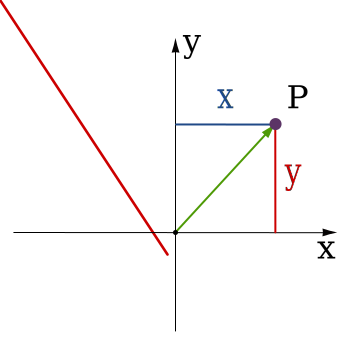
\includegraphics[width=0.25\columnwidth]{Chap07VectorSpaceRnPart1/Coord-XYWikiMediaCommons.png}}%
\caption[]{Images of the $xy$-plane with Cartesian coordinates $x$ and $y$, courtesy of the WikiMedia Commons. (a) shows a vector drawn to the \textbf{point} $(2,3)$ and labeled suggestively as a vector from the origin O to point A. (b) shows a \textbf{point} $P$ represented with coordinates $(x,y)$, also with a vector drawn to it. These are both fine interpretations of vectors. In ROB 101, points and vectors are the same thing: an ordered list of numbers.}
    \label{fig:2Dvectors}
\end{figure}




Figure~\ref{fig:2Dvectors} shows two geometric depictions of vectors in 2D, one emphasizing a vector as a directed line segment from the origin $O$ to a point $A$ located at $(2,3)$, while the second is a directed line segment from the origin $O$ to a point $P$ located at $(x,y)$. Both of these are fine interpretations of vectors. In $\real^2$, graphical depictions of vectors are relatively straightforward to understand. Figure~\ref{fig:3DSpace} illustrates so-called unit vectors along the $xyz$-axes in $\real^3$, while Fig.~\ref{fig:xyzP} shows a point in $\real^3$ with Cartesian coordinates $(x,y,z)$. These depictions of vectors and points in $\real^3$ are fairly simple, but it is not hard to give other examples in $\real^3$ that are harder to ``picture'' as a 2D-image, which is all we can show on a sheet of paper. So yes, it easy to get lost in 3D-space and if you have a hard time ``imagining'' (that is, representing visually in your head for the purpose of building intuition) objects in 3D, you are not alone. Anyone want to try $\real^{27}$, that is, 27D-space?\\

In ROB 101, points in $\real^n$ are vectors. We treat points and vectors as being different ways of representing the same mathematical object: an ordered list of numbers. Don't get hung up on the geometric aspect of vectors. In Physics, Dynamics, and Electromagnetics courses, you'll be challenged to ``imagine'' vectors in 3D. Deal with it there. For now, it is OK to think of vectors as lists of numbers that obey some basic algebraic relationships and nothing more. Besides, when dealing with a vector that has hundreds of components, what else can you do?

\begin{figure}[htb]%
\centering
\subfloat[]{%
    \label{fig:3DSpace}%
	\centering
\includegraphics[width=0.35\columnwidth]{graphics/Chap07VectorSpaceRnPart1/ijk_Unit-vectors-in-Cartesian-CoordCreativeCommonsWikimediaCommons02.png}}%
\hspace{100pt}%
\subfloat[]{%
    \label{fig:xyzP}%
	\centering
\includegraphics[width=0.35\columnwidth]{graphics/Chap07VectorSpaceRnPart1/3DSpacexyzCreativeCommons02.png}}%
\caption[]{Images of 3D space with Cartesian coordinates $x$, $y$, and $z$ using two different color schemes. (a), courtesy of WikiMedia Commons, emphasizes that the vector $a = a_x + a_y+a_z$ is the sum of three vectors lying along the $x$-axis, $y$-axis, and $z$-axis, respectively. (b), courtesy of Prof. Maani Ghaffari, emphasizes that the point $P=(x,y,z)$ has an $x$-component $P_x$, a $y$-component $P_y$, and $z$-component $P_z$. In ROB 101, points and vectors are the same thing. Moreover, we do not rely on your ability to imagine vectors in $n$-dimensional space for $n >2$.}
    \label{fig:3Dvectors}
\end{figure}

\vspace*{0.5cm}

\begin{tcolorbox}[title=\textbf{3 Special Vectors in $\real^3$}]
Figure~\ref{fig:3DSpace} defines ``unit'' vectors $\widehat{i}$, $\widehat{j}$, and $\widehat{k}$. You will see these a lot in Physics.
The more accepted mathematical notation in Linear Algebra is
$$e_1 := \begin{bmatrix} 1  \\ 0\\ 0\end{bmatrix},~e_2 := \begin{bmatrix} 0 \\ 1 \\ 0 \end{bmatrix}, ~\text{and}~ e_3 := \begin{bmatrix}0 \\ 0\\ 1 \end{bmatrix}.$$
\end{tcolorbox}


\vspace*{.5cm}

\begin{tcolorbox}[title=\textbf{Properties of Vector Addition and Scalar Times Vector Multiplication}]

 \begin{enumerate}
        \item Addition is commutative: For any $x \in \real^n$ and $y \in \real^n$, 
        $$x+y = y + x.$$
        \item Addition is associative: For any  $x \in \real^n$,  $y \in \real^n$  and $z \in \real^n$, 
        $$\left(x+y\right)+z = x+ \left( y + z \right).$$
        
        \item Scalar multiplication is associative: For any $\alpha \in \real$, $\beta \in \real$, and any $x \in \real^n$ in 
        $$\alpha \left(\beta  x \right) = \left(\alpha \beta\right) x.$$
        \item Scalar multiplication is distributive: For any $\alpha \in \real$, $\beta\in \real$ and for any $x \in \real^n$, $y\in \real^n$, 
        $$(\alpha + \beta ) x= \alpha x + \beta x ,$$
        and 
         $$\alpha \left(x + y \right) = \alpha x + \alpha y.$$
    \end{enumerate}
    
All of these properties follow from the corresponding properties for real numbers. Hence, there is no real reason to make a big deal about them. You've been adding vectors and multiplying them by constants in Julia for several weeks now!

\end{tcolorbox}



\vspace*{0.5cm}
\section{The Notion of Linear Combinations}

Sums of vectors times scalars are called linear combinations. We'll introduce the concept in two ways: first by studying what $Ax$ really means in terms of the columns of $A$ and the components of $x$, and in a second pass, a more ``pure'' or ``abstract'' definition in $\real^n$. If you enjoyed the previous 3Blue1Brown video, then I suggest you check out this one as well \url{https://www.youtube.com/watch?v=k7RM-ot2NWY}.

\subsection{Linear combinations through the lens of Ax=b}
\label{sec:LinComboExistSolutinsLensAxb}

 Let's consider $Ax=b$ and see if we truly understand the product of an $n \times m$ matrix $A$ and an $m \times 1$ column vector $x$, and then the equation $Ax=b$! We write 
 \begin{equation}
\label{eq:MatrixFromLinearIndependence_proTip}    
A=\left[\begin{array}{cccc} a_{11}& a_{12}& \cdots & a_{1m} \\
 a_{21}& a_{22}& \cdots & a_{2m}  \\
 \vdots & \vdots&  \ddots & \vdots \\
 a_{n1}& a_{n2}& \cdots & a_{nm} 
 \end{array}\right]~~\text{and}~~\left[ \begin{array}{c} x_1 \\ x_2 \\
\vdots \\ x_m   \end{array} \right]. 
 \end{equation}
Then, using our column times row method for matrix multiplication, we have
\begin{equation}
    \label{eq:bIsLinearCombinationColumnsA}
A x = \left[\begin{array}{cccc} a_{11}& a_{12}& \cdots & a_{1m} \\
 a_{21}& a_{22}& \cdots & a_{2m}  \\
 \vdots & \vdots&  \ddots & \vdots \\
 a_{n1}& a_{n2}& \cdots & a_{nm} 
 \end{array}\right] \left[ \begin{array}{c} x_1 \\ x_2 \\
\vdots \\ x_m   \end{array} \right] = \begin{bmatrix} a_{11} \\ a_{21}\\ \vdots \\ a_{n1} \end{bmatrix} {x}_1 +  \begin{bmatrix} a_{12} \\ a_{22}\\ \vdots \\ a_{n2} \end{bmatrix} {x}_2 + \cdots + \begin{bmatrix} a_{1m} \\ a_{2m}\\ \vdots \\ a_{nm} \end{bmatrix} {x}_m.
\end{equation}
If the above is not clicking for you, go back and look at our second method for matrix multiplication in Chapter~\ref{chap:MatrixMultiplication}. Note that the rows of the vector $x$ are simply its components; another way to look at is, because $x$ is $m \times 1$, its rows are $1 \times 1$.\\

The next step is to move the $x_i$ in front of the column vectors of $A$, as in
$$Ax = {x}_1 \begin{bmatrix} a_{11} \\ a_{21}\\ \vdots \\ a_{n1} \end{bmatrix}  + {x}_2  \begin{bmatrix} a_{12} \\ a_{22}\\ \vdots \\ a_{n2} \end{bmatrix}  + \cdots + {x}_m \begin{bmatrix} a_{1m} \\ a_{2m}\\ \vdots \\ a_{nm} \end{bmatrix}. $$
Because we are used to thinking of the $x_i$ as variables or unknowns, let's substitute in a ``numerical'' value, such as $\alpha_i.$ Of course, this has not changed anything, but it might look different to you,
$$A\left[ \begin{array}{c} \alpha_1 \\ \alpha_2\\
\vdots \\ \alpha_m  \end{array} \right] = \alpha_1 \begin{bmatrix} a_{11} \\ a_{21}\\ \vdots \\ a_{n1} \end{bmatrix}  + \alpha_2  \begin{bmatrix} a_{12} \\ a_{22}\\ \vdots \\ a_{n2} \end{bmatrix}  + \cdots + \alpha_m \begin{bmatrix} a_{1m} \\ a_{2m}\\ \vdots \\ a_{nm} \end{bmatrix}. $$

\begin{tcolorbox}[sharp corners, colback=green!30, colframe=green!80!blue,title=\textbf{Linear Combination of the Columns of A}]

\textbf{Definition} The following sum of scalars times vectors,
\begin{equation}
    \label{eq:EarlyDefLinearCombination}
    \alpha_1 \begin{bmatrix} a_{11} \\ a_{21}\\ \vdots \\ a_{n1} \end{bmatrix}  + \alpha_2  \begin{bmatrix} a_{12} \\ a_{22}\\ \vdots \\ a_{n2} \end{bmatrix}  + \cdots + \alpha_m \begin{bmatrix} a_{1m} \\ a_{2m}\\ \vdots \\ a_{nm} \end{bmatrix},
\end{equation}
is called a \textbf{linear combination} of the columns of $A$. When we set $A\alpha = b$, and turn it around as $b =A \alpha$, we arrive at an important \textbf{Fact:} a vector $\alpha \in \real^m$ is a solution to $Ax=b$ (that is, $A \alpha = b$) if, and only if
\begin{equation}
    \label{eq:EarlyDefLinearCombinationWithb}
   b= \alpha_1 \begin{bmatrix} a_{11} \\ a_{21}\\ \vdots \\ a_{n1} \end{bmatrix}  + \alpha_2  \begin{bmatrix} a_{12} \\ a_{22}\\ \vdots \\ a_{n2} \end{bmatrix}  + \cdots + \alpha_m \begin{bmatrix} a_{1m} \\ a_{2m}\\ \vdots \\ a_{nm} \end{bmatrix},
\end{equation}
that is, $b$ can be expressed as a linear combination of the columns of $A$.
We will revisit this later, but \eqref{eq:EarlyDefLinearCombinationWithb} is a primary motivation for introducing the notion of linear combinations.
\end{tcolorbox}

\subsection{Linear Combinations in $\real^n$}

\begin{tcolorbox}[title=\textbf{Linear Combination}]
A vector $v\in \real^n$ is a \textbf{linear combination of} $\{u_1, u_2, \ldots, u_m\} \subset \real^n$ if there exist real numbers $\alpha_1, \alpha_2, \ldots, \alpha_m$ such that
\begin{equation}
    \label{eq:DefLinearCombinationRn}
    v = \alpha_1 u_1 + \alpha_2 u_2 + \cdots + \alpha_m u_m.
\end{equation}

\end{tcolorbox}

\vspace*{0.5cm}

\begin{example}
\label{ex:LinearComboA1}
Because 
$$\underbrace{\begin{bmatrix} -3 \\  -5 \\ -7\end{bmatrix}}_{v}=2\underbrace{\begin{bmatrix} 3 \\  2 \\ 1\end{bmatrix}}_{u_1} - 9 \underbrace{ \begin{bmatrix} 1 \\  1 \\ 1\end{bmatrix}}_{u_2},$$
we have that $v$ is a linear combination of $\{u_1, u_2\}$.
\end{example}

When you are given the coefficients, it is easy to observe that a given vector is a linear combination of other vectors. But when you have to check if such coefficients exist or do not exist, then it's just a wee bit more challenging!
\vspace*{0.5cm}

\begin{example}
\label{ex:LinearComboA2}
Is the vector $v= \begin{bmatrix} 4 \\  4 \\ 4\end{bmatrix}$ a linear combination of 
$$u_1=\left[\begin{array}{r} 3 \\ 1\\ -1  \end{array} \right]~~\text{and}~~u_2=\left[\begin{array}{r} 2 \\ -2\\ 1  \end{array} \right]? $$
\end{example}

\textbf{Solution:} The vector $v$ is a linear combination of the vectors $u_1$ and $u_2$ if, and only if, there exist real numbers $\alpha_1$ and $\alpha_2$ such that
\begin{equation}
\label{eq:LinearCombination}
   \alpha_1 u_1 + \alpha_2 u_2 = v. 
\end{equation} 
What we have done here is apply\footnote{In the beginning, many of us are confused about how to go about solving a problem. Sound advice is to start with the definitions at your disposal. Then try to turn the definition into a set of equations to be solved.} \textbf{the definition of a linear combination.}
So, we write down the linear equations corresponding to \eqref{eq:LinearCombination}, namely
\begin{equation}
\label{eq:CheckLinearCombinationEquations}
\begin{aligned}
    \alpha_1 \left[ \begin{array}{r} 3 \\ 1 \\ -1   \end{array} \right] + \alpha_2 \left[ \begin{array}{r} 2 \\ -2 \\ 1   \end{array} \right] &= \left[ \begin{array}{r} 4 \\ 4 \\ 4   \end{array} \right]\\
   & \Updownarrow \\
    \left[ \begin{array}{rr} 3 & 2\\ 1  & -2\\ -1  & 1 \end{array} \right]  \left[ \begin{array}{r} \alpha_1 \\ \alpha_2 \end{array} \right] &= \left[ \begin{array}{r} 4 \\ 4 \\ 4   \end{array} \right]
\end{aligned}
\end{equation}
and see if we can find a solution for the \textbf{unknowns} $\alpha_1$ and $\alpha_2$! What makes this look hard is that we have a non-square (rectangular) system of linear equations, namely, three equations and two unknowns.\\

What are the three equations? They may look more familiar to you if we write them out like this,
\begin{align*}
   3 \alpha_1 + 2 \alpha_2 &=4 \\
   \alpha_1 - 2 \alpha_2 &= 4\\
   -\alpha_1 + \alpha_2 &= 4.
\end{align*}

A systematic way to approach such problems is to observe that if $\alpha_1$ and $\alpha_2$ are to simultaneously satisfy all three equations, then they must necessarily satisfy any two of them. Moreover, if you find that the solution to the resulting square system of two equations and two unknowns is unique, then two things are possible:
\begin{itemize}
    \item the solution of the smaller square system of equations also satisfies the equation(s) you did not use, giving you a solution to the full set of equations, or
    \item the solution of the smaller square system of equations does not satisfy the equation(s) you did not use, telling you that the full set of equations is inconsistent and does not have a solution.
\end{itemize}

In our case, if we remove the last equation, we have 
\begin{equation}
\label{eq:CheckLinearCombinationEquationsKeepTwo}
\begin{aligned}
       \left[ \begin{array}{rr} 3 & 2\\ 1  & -2 \end{array} \right]  \left[ \begin{array}{r} \alpha_1 \\ \alpha_2 \end{array} \right] &= \left[ \begin{array}{r} 4 \\ 4   \end{array} \right],
\end{aligned}
\end{equation}
and we observe that the matrix multiplying the vector of unknowns has determinant $-8$, and thus \eqref{eq:CheckLinearCombinationEquationsKeepTwo} has a unique solution. A bit of matrix magic with our formula for a $2 \times 2$ inverse gives
 $$\alpha_1=2~~\text{and}~\alpha_2=-1. $$
 Do these values satisfy the equation we did not use, namely, the last row of \eqref{eq:CheckLinearCombinationEquationsKeepTwo},
 $$\left[ \begin{array}{rr} -1  & 1 \end{array} \right]  \left[ \begin{array}{r} \alpha_1 \\ \alpha_2 \end{array} \right] = \left[ \begin{array}{r} 4\end{array} \right]? $$
Clearly not, because $-1 \alpha_1 + \alpha_2 = -3 \neq 4,$ and
\textbf{hence, $v$ is NOT a linear combination of $u_1$ and $u_2$.} 

\vspace*{0.5cm}

\begin{tcolorbox}
The key point is that $\alpha_1$ and $\alpha_2$ must satisfy all three equations in \eqref{eq:CheckLinearCombinationEquations}. It does not matter in what order we use the equations when seeking a solution. To illustrate that, we'll first solve the last two equations, 
\begin{align*}
     \alpha_1 - 2 \alpha_2 &= 4 \\
 -\alpha_1 + \alpha_2 &= 4,
\end{align*}
which yields, $\alpha_1=-12$ and $\alpha_2=-8$. We then check if these values satisfy the first equation
$$ 3\alpha_1 +2 \alpha_2 = 4 \iff -36  - 16 = 4 \iff -52= 4,$$
which is false, and therefore, $v$ is NOT a linear combination of $u_1$ and $u_2$.
\end{tcolorbox}

\vspace*{.5cm} 

\textbf{Rework the problem:} Let's keep $u_1$ and $u_2$ as given and change $v$ to
$$\tilde{v}=  \left[ \begin{array}{r} 0 \\ -8 \\ 5   \end{array} \right].$$
Applying the above strategy to the equations
\begin{align*}
   3 \alpha_1 + 2 \alpha_2 &=0\\
   \alpha_1 - 2 \alpha_2 &= -8\\
   -\alpha_1 + \alpha_2 &= 5
\end{align*}
yields $\alpha_1=-2$ and $\alpha_2=3$, as you can verify by direct substitution. \textbf{Hence, $\tilde{v}$ is a linear combination of $u_1$ and $u_2$.} \Qed

\vspace*{0.5cm}

\textbf{Remark:} Checking whether a given vector can be written as a linear combination of other vectors always comes down to solving a system of linear equations. If that system is square with a non-zero determinant, then solving the system of equations is cake. Otherwise, solving the equations by hand is mostly painful. \textbf{We will need to develop a better way to check if a vector is, or is not, a linear combination of other vectors!}

\section{Existence of Solutions to Ax=b}
\label{sec:UniquenessSolutions}

Because it is so important, we now revisit the relation of linear combinations to the existence of solutions to systems of linear equations. We want to make sure you did NOT miss something important when reading Chapter~\ref{sec:LinComboExistSolutinsLensAxb}. If you are confident of your knowledge, then feel free to move on to the next section. Otherwise, please read on!\\

Let $A$ be an $n \times m$ matrix, not necessarily square, as in \eqref{eq:ColumnsOfMatrixVectorsRn}. Recall that columns of $A$ and vectors in $\real^n$ are the same thing. We write out $Ax=b$ is all its glory, 
\begin{equation}
\label{eq:ExistenceSolutionsNonsquare}    
 \underbrace{\left[\begin{array}{cccc} a_{11}& a_{12}& \cdots & a_{1m} \\
 a_{21}& a_{22}& \cdots & a_{2m}  \\
 \vdots & \vdots&  \ddots & \vdots \\
 a_{n1}& a_{n2}& \cdots & a_{nm} 
 \end{array}\right] }_{A} \underbrace{\left[ \begin{array}{c} x_1 \\ x_2 \\
\vdots \\ x_m   \end{array} \right]}_{x} = \underbrace{\left[ \begin{array}{c} b_1 \\ b_2 \\ \vdots \\ b_n  \end{array} \right]}_{b}.
\end{equation}

\vspace*{.5cm}
\begin{tcolorbox}[sharp corners, colback=green!30, colframe=green!80!blue, title=\textbf{\large Existence of Solutions}] 
The equation $Ax=b$ has a solution if, and only if, $b$ can be written as a linear combination of the columns of $A$.
\end{tcolorbox}

\vspace{0.5cm}
\begin{tcolorbox}%[title=\textbf{Why it is true}]
\textbf{The following is more or less a proof:} Suppose that $\bar{x}$ satisfies $A \bar{x} =b$, which is the same thing as saying $\bar{x}$ is a solution of $Ax=b$. Then, doing the indicated multiplication of $A \bar{x}$ via our now favorite method, the columns of $A$ times the rows of the vector $\bar{x}$, which are its scalar entries $\bar{x}_i$, yields
\begin{equation}
    \label{eq:bIsLinearCombinationColumnsA02}
\begin{bmatrix} a_{11} \\ a_{21}\\ \vdots \\ a_{n1} \end{bmatrix} \bar{x}_1 +  \begin{bmatrix} a_{12} \\ a_{22}\\ \vdots \\ a_{n2} \end{bmatrix} \bar{x}_2 + \cdots + \begin{bmatrix} a_{1m} \\ a_{2m}\\ \vdots \\ a_{nm} \end{bmatrix} \bar{x}_m = \begin{bmatrix} b_1 \\ b_2\\ \vdots \\ b_m \end{bmatrix}
\end{equation}
Exchanging the two sides of the equal sign and moving the scalars $\bar{x}_i$ to the front of the vectors give
\begin{equation}
    \label{eq:bIsLinearCombinationColumnsAflipped}
 \begin{bmatrix} b_1 \\ b_2\\ \vdots \\ b_m \end{bmatrix} = \bar{x}_1 \begin{bmatrix} a_{11} \\ a_{21}\\ \vdots \\ a_{n1} \end{bmatrix}+ \bar{x}_2 \begin{bmatrix} a_{12} \\ a_{22}\\ \vdots \\ a_{n2} \end{bmatrix} + \cdots + \bar{x}_m \begin{bmatrix} a_{1m} \\ a_{2m}\\ \vdots \\ a_{nm} \end{bmatrix};
\end{equation}
in other words, $b$ is a linear combination of the columns of $A$. The other way around works as well: if we manage to write 
$$b = c_1  a_1^{\rm col} + c_2 a_2^{\rm col} + \cdots c_m a_m^{\rm col}$$
for some real numbers $c_i \in \real$, then $\bar{x}=\begin{bmatrix} c_1 & c_2 & \cdots & c_m \end{bmatrix}^\top$ satisfies $A \bar{x}=b$, and hence it is a solution to $Ax=b$. \\

Recall that $a_j^{\rm col}:=\begin{bmatrix} a_{ij} & a_{2j}  & \cdots & a_{nj} \end{bmatrix}^\top, 1 \le j \le m.$
\end{tcolorbox}

A weakness of the above result is that we do not yet have an effective means for checking whether or not a given vector is a linear combination of a specified set of vectors. We will solve this problem too, a little bit later in the Chapter. All we have done so far is indicate that the concept of a linear combination is related to the existence of a solution to a corresponding system of linear equations. \textbf{The result is mainly conceptual in that we have not yet provided a practical way to check this in code. That will come, though! Long Live the LU Factorization!}


\section{Linear Independence of a Set of Vectors}

\subsection{Preamble}
The concept of \textit{linear independence}, or its logical opposite, the concept of \textit{linear dependence}, is one of the most important ideas in all of linear algebra. In the beginning, most of us struggle with two things: (1) why is the property of linear independence so important; and (2), how do you test for it? In this section, we highlight the importance of linear independence of vectors by relating it to uniqueness of solutions to $\mathbf{Ax=0}$ and eventually, to uniqueness of solutions to $\mathbf{Ax=b}$. We'll also show that our friend, the LU Factorization, makes testing for linear independence very straightforward. 

\subsection{Linear Independence through the Lens of Ax=0}

Let $A$ be an $n \times m$ matrix. We say that $x\in \real^m$ is a \textbf{nontrivial solution} to $Ax=0_{n \times 1}$ if
\begin{itemize}
    \item $Ax=0_{n \times 1}$ ($x$ is a solution), and 
    \item $x\neq0_{m \times 1} $ ($x$ is not the zero vector in $\real^m)$. 
\end{itemize}
Because $x=0$ is always a solution to $Ax=0$, for it to be the \textbf{unique solution}, there must not be a non-trivial solution to $Ax=0.$\\

Why are we making such a big deal about this? Because uniqueness is a desirable property and we want to learn how to check for it even in the case of rectangular systems of equations\footnote{Recall, when $A$ is square, uniqueness is equivalent to $\det(A)\neq 0$.}. Our immediate goal is to see what this means in terms of the columns of $A$, just as we did when introducing the notion of a linear combination. \\

To see what it means to have ``non-trivial solutions'' to $Ax=0_{n \times 1}$, once again, we replace $x \in \real^m$ by a vector $\alpha \in \real^m$ and write
 \begin{equation}
\label{eq:MatrixFromLinearIndependence_proTipB}    
A=\left[\begin{array}{cccc} a_{11}& a_{12}& \cdots & a_{1m} \\
 a_{21}& a_{22}& \cdots & a_{2m}  \\
 \vdots & \vdots&  \ddots & \vdots \\
 a_{n1}& a_{n2}& \cdots & a_{nm} 
 \end{array}\right]~~\text{and}~~\alpha =\left[ \begin{array}{c} \alpha_1 \\ \alpha_2 \\
\vdots \\ \alpha_m   \end{array} \right]. 
 \end{equation}
Then, using our column times row method for matrix multiplication, and re-arranging terms a bit as we did in Chapter~\ref{sec:LinComboExistSolutinsLensAxb},
\begin{equation}
    \label{eq:LinearIndepColumnsA01}
    \begin{aligned}
A \alpha &= \left[\begin{array}{cccc} a_{11}& a_{12}& \cdots & a_{1m} \\
 a_{21}& a_{22}& \cdots & a_{2m}  \\
 \vdots & \vdots&  \ddots & \vdots \\
 a_{n1}& a_{n2}& \cdots & a_{nm} 
 \end{array}\right] \left[ \begin{array}{c} \alpha_1 \\ \alpha_2\\
\vdots \\ \alpha_m  \end{array} \right] \\
& = \alpha_1 \begin{bmatrix} a_{11} \\ a_{21}\\ \vdots \\ a_{n1} \end{bmatrix}  + \alpha_2  \begin{bmatrix} a_{12} \\ a_{22}\\ \vdots \\ a_{n2} \end{bmatrix}  + \cdots + \alpha_m \begin{bmatrix} a_{1m} \\ a_{2m}\\ \vdots \\ a_{nm} \end{bmatrix}.
    \end{aligned}
\end{equation}
Hence, $A\alpha = 0_{n \times 1}$ if, and only if, 
\begin{equation}
    \label{eq:LinearIndepColumnsA02}
    \begin{aligned}
\alpha_1 \begin{bmatrix} a_{11} \\ a_{21}\\ \vdots \\ a_{n1} \end{bmatrix}  + \alpha_2  \begin{bmatrix} a_{12} \\ a_{22}\\ \vdots \\ a_{n2} \end{bmatrix}  + \cdots + \alpha_m \begin{bmatrix} a_{1m} \\ a_{2m}\\ \vdots \\ a_{nm} \end{bmatrix} & = \begin{bmatrix} 0 \\ 0\\ \vdots \\ 0 \end{bmatrix}_{n \times 1}.
    \end{aligned}
\end{equation}
Our takeaway is, $\alpha = 0_{m \times 1}$ is the unique solution to $A\alpha=0$ if, and only if, the only way we can add up the columns of $A$ and obtain the zero vector in $\real^n$ is with 
$$\alpha_1=0, \alpha_2=0, \ldots, \alpha_m=0. $$
Or equivalently, $A\alpha = 0$ has a non-trivial solution $\alpha \neq 0_{m \times 1}$, if, and only if, there exists real numbers $\alpha_1, \alpha_2, \ldots, \alpha_m$, \textbf{NOT ALL ZERO}, such that \eqref{eq:LinearIndepColumnsA02} is satisfied.

\subsection{Linear Independence in $\real^n$ (and why theory matters)}

The definition of linear independence of an ``abstract'' set of vectors in $\real^n$ is 100\% motivated by the study above on the uniqueness of solutions to $Ax=0.$ Of course, vectors in $\real^n$ are columns of $n \times m$ matrices, so who's to say what is abstract and what is not!

\vspace*{0.5cm}

\begin{tcolorbox}[sharp corners, colback=green!30, colframe=green!80!blue, title=\textbf{Linear Independence of a Set of Vectors}]
 The set of vectors $\{v_1, v_2, ..., v_m \} \subset \real^n$ is \textbf{linearly dependent} if there exist real numbers $\alpha_1, \alpha_2, \ldots, \alpha_m$ \textbf{NOT ALL ZERO} yielding a linear combination of vectors that adds up to the zero vector,
\begin{equation}
    \alpha_1 v_1 + \alpha_2 v_2 + \ldots + \alpha_m v_m =0_{n \times 1}.
\end{equation}

On the other hand, the vectors $\{v_1, v_2, ..., v_m \}$ are \textbf{linearly independent} if the \textbf{only} real numbers $\alpha_1, \alpha_2, \ldots, \alpha_m$ yielding a linear combination of vectors that adds up to the zero vector,
\begin{equation}
    \alpha_1 v_1 + \alpha_2 v_2 + \ldots + \alpha_m v_m =0_{n \times 1},
    \end{equation}
are $\boldsymbol{\alpha}_1= \mathbf{0}, \boldsymbol{\alpha}_2=\mathbf{0}, \ldots, \boldsymbol{\alpha}_m=\mathbf{0}.$\\

\textbf{Concise Definition of Linear Independence:} 
$$\alpha_1 v_1 + \alpha_2 v_2 + \ldots + \alpha_m v_m =0_{n \times 1}  \iff \begin{bmatrix} \alpha_1 \\ \alpha_2 \\ \vdots \\ \alpha_m \end{bmatrix} = \begin{bmatrix} 0 \\ 0 \\ \vdots \\ 0 \end{bmatrix}= 0_{m \times 1}.$$
\end{tcolorbox}

\vspace*{.5cm}
\begin{example} 
\label{ex:LinearIndep02} By applying the definition, determine if the set of vectors
$$v_1 = \left[ \begin{array}{r} \sqrt{2} \\0\\  0  \end{array} \right]  , v_2 = \left[ \begin{array}{r}  4 \\ 7  \\0  \end{array} \right], v_3 = \left[ \begin{array}{r} 3 \\ 1 \\ -1   \end{array} \right] $$
is linearly independent or dependent.
\end{example}

\textbf{Solution:} We form the linear combination and do the indicated multiplications and additions
\begin{equation}
\label{eq:LinearIndependenceExample02}
    \alpha_1 v_1 + \alpha_2 v_2 + \alpha_3 v_3 = 
    \alpha_1 \left[ \begin{array}{r} \sqrt{2} \\0\\ 0  \end{array} \right] 
+ \alpha_2 \left[ \begin{array}{r}  4 \\ 7 \\ 0  \end{array} \right] 
+ \alpha_3 \left[ \begin{array}{r} 3 \\ 1 \\ -1   \end{array} \right]  = \left[ \begin{array}{r}  \sqrt{2}\  \alpha_1  + 4\ \alpha_2 + 3\ \alpha_3\\7 \ \alpha_2 + \alpha_3\\  -1\ \alpha_3 \end{array} \right].
\end{equation}
Setting the right hand side of \eqref{eq:LinearIndependenceExample02} to the zero vector yields
\begin{equation}
\label{eq:LinearIndependenceExample02b}
   \left[ \begin{array}{r}  \sqrt{2}\  \alpha_1  + 4\ \alpha_2 + 3\ \alpha_3\\7 \ \alpha_2 + \alpha_3\\  -1\ \alpha_3 \end{array} \right] = \left[ \begin{array}{r} 0 \\ 0 \\ 0   \end{array} \right].
\end{equation}
This is one of our friendly triangular systems of linear equations which we can solve via back substitution. We see immediately that the only solution to the bottom equation is $\alpha_3=0$, the only solution to the middle equation is then $\alpha_2 = 0$, and finally, the only solution to the top equation is $\alpha_1=0$. Hence, the only solution to 
$$ \alpha_1 v_1 + \alpha_2 v_2 + \alpha_3 v_3 =0 $$
is $\alpha_1=0$, $\alpha_2 = 0$, and $\alpha_3=0$, and hence the set of vectors  $ \{v_1, v_2, v_3 \} $ is linearly independent.\\

The above analysis becomes even more clear when we write \eqref{eq:LinearIndependenceExample02b} as
\begin{equation}
\label{eq:LinearIndependenceExample02c}
   \left[ \begin{array}{ccr}  \sqrt{2} &  4 &  3 \\ 0 & 7  & 1 \\ 0 & 0 & -1  \end{array} \right]\left[ \begin{array}{r} \alpha_1 \\ \alpha_2 \\ \alpha_3   \end{array} \right] = \left[ \begin{array}{r} 0 \\ 0 \\ 0   \end{array} \right] .
\end{equation}
We see that the matrix is square with a non-zero determinant, and hence we know it has a unique solution. 
 \Qed \\
 
 \vspace{.5cm}

\begin{example} 
\label{ex:LinearIndep00} By applying the definition, determine  if the set of vectors $$ v_1 = \left[ \begin{array}{r} 1 \\2\\  3 \end{array} \right]  , v_2 = \left[ \begin{array}{r}  1 \\ -2  \\-4  \end{array} \right] $$
is linearly independent or dependent.
\end{example}

\textbf{Solution:} We seek to determine if there are non-zero coefficients $\alpha_1$ and $\alpha_2$ resulting in a linear combination that forms the zero vector in $\real^3$,
\begin{equation}
\label{eq:LinearIndependenceExample00a}
    \alpha_1 v_1 + \alpha_2 v_2  = 
    \alpha_1 \left[ \begin{array}{r} 1 \\2\\  3  \end{array} \right] 
+ \alpha_2 \left[ \begin{array}{r}  1 \\ -2  \\-4  \end{array} \right] =  \left[ \begin{array}{r} \alpha_1 + \alpha_2\\ 2 \alpha_1 -2  \alpha_2 \\ 3 \alpha_1 -4 \alpha_2 \end{array} \right] = \left[ \begin{array}{r} 0 \\ 0 \\0\end{array} \right].
\end{equation}
We observe that we have three equations in two unknowns and no obvious triangular structure to help us! What do we do? Well, if we can take any two of the three equations and show that the only solution is the trivial solution,  $\alpha_1=0$ and $\alpha_2=0$, then we are done, because the trivial solution will always satisfy the remaining equation. Please check this reasoning out for yourself.\\

We arbitrarily group the equations into the first two equations and then the last equation, as follows 
\begin{align}
\label{eq:LinearIndependenceExample00b1}
    \alpha_1 \left[ \begin{array}{r} 1 \\2\\ \end{array} \right] 
+ \alpha_2 \left[ \begin{array}{r}  1 \\ -2   \end{array} \right] &= \left[ \begin{array}{r} 0 \\ 0 \end{array} \right] \\
\label{eq:LinearIndependenceExample00b2}
\alpha_1 \left[ \begin{array}{r} 3 \end{array} \right] + \alpha_2 \left[ \begin{array}{r} -4\end{array} \right] &= 0.
\end{align}

We can rewrite \eqref{eq:LinearIndependenceExample00b1} in the form $A \alpha=b$
\begin{equation}
\label{eq:LinearIndependenceExample00c1}
   \underbrace{\left[ \begin{array}{rr} 1 & 1\\2 & -2 \end{array} \right]}_{A} 
\underbrace{\left[ \begin{array}{c} \alpha_1 \\ \alpha_2 \end{array} \right]}_{\alpha} =  \underbrace{ \left[ \begin{array}{r} 0 \\ 0 \end{array} \right]}_{b}.
\end{equation}
We note that $\det(A) = (1)(-2)-(1)(2) = -4 \neq 0$, and hence \eqref{eq:LinearIndependenceExample00c1} has a unique solution. Because $\alpha_1=0$ and $\alpha_2=0$ is a solution and the solution is unique, we know that there cannot exist a different set of non-zero  $\alpha_1$ and $\alpha_2$ that also solve the equation. We, therefore, conclude that the vectors $\{v_1, v_2\}$ are linearly independent. \\

\textbf{Remark:} Let's step back and see what is going on here. We have three equations and two unknowns. The trivial  solution is always a solution to the full set of equations. We wonder if there is any other solution. If we make a choice of two of the equations, so that we have a more manageable square system of equations, and then find that those two equations constrain the solution to being the trivial solution, we are done! (Why, because the trivial solution will automatically satisfy the remaining equation and it is then the only solution that satisfies all three equations.)
 \Qed\\
 
 
That was a lot of work! It does not seem like it will scale to bigger sets of vectors.  We'll do one more example to convince you that we are in dire need of a \textbf{Pro Tip!}

\vspace*{0.5cm}

\begin{example} 
\label{ex:LinearIndep01} By applying the definition, determine  if the vectors 
$$v_1 = \left[ \begin{array}{r} 1 \\2\\  3 \\1  \end{array} \right]  , v_2 = \left[ \begin{array}{r}  0 \\ -2  \\4 \\ 5  \end{array} \right], v_3 = \left[ \begin{array}{r} 2 \\ 6 \\ 2  \\ -3 \end{array} \right] $$
are linearly independent or dependent.
\end{example}

\textbf{Solution:} We form the linear combination and set it equal to zero,
\begin{equation}
\label{eq:LinearIndependenceExample01}
    \alpha_1 v_1 + \alpha_2 v_2 + \alpha_3 v_3 = 
    \alpha_1 \left[ \begin{array}{r} 1 \\2\\  3 \\1  \end{array} \right] 
+ \alpha_2 \left[ \begin{array}{r}  0 \\ -2  \\4 \\ 5  \end{array} \right]
+ \alpha_3 \left[ \begin{array}{r} 2 \\ 6 \\ 2  \\ -3 \end{array} \right]  = \left[ \begin{array}{r} \alpha_1  +2\ \alpha_3 \\ 2 \alpha_1 -2 \alpha_2 + 6 \alpha_3\\ 3 \alpha_1+ 4 \alpha_2 +  2 \alpha_3  \\ \alpha_1+ 5 \alpha_2 -3 \alpha_3 \end{array} \right] = \left[ \begin{array}{r}  0 \\ 0 \\0 \\0  \end{array} \right].
\end{equation}
\textbf{We must check whether or not there are \textit{non-trivial} solutions to} \eqref{eq:LinearIndependenceExample01}, where non-trivial means at least one of the coefficients $\alpha_1$,  $\alpha_2$, or  $\alpha_3$ is non-zero.\\ 

We observe that we have four equations in three unknowns. Similar to Example~\ref{ex:LinearIndep00}, we could select any three of the four equations, solve those three, and then see if that solution is compatible with the remaining equation. Once again, this will be a lot of work. We'll save ourselves the effort and let you verify that $\alpha_1=2, \alpha_2=-1, \alpha_3 = -1$ is a non-trivial solution to \eqref{eq:LinearIndependenceExample01} and hence the vectors $v_1, v_2, v_3$ are linearly dependent. \textbf{Where is that Pro Tip?} \Qed\\



% % The method in Example~\ref{ex:LinearIndep02} is completely general, and we summarize it in the following. 
% \vspace*{0.5cm}
% \begin{tcolorbox}[sharp corners, colback=green!30, colframe=green!80!blue, title=\textbf{\large Relating Linear Independence of Vectors to a System of Linear Equations}]
% Consider the vector space $\real^n$ and a set of vectors 
% $$\left\{v_1=\begin{bmatrix} a_{11} \\ a_{21}\\ \vdots \\ a_{n1} \end{bmatrix}, v_2=\begin{bmatrix} a_{12} \\ a_{22}\\ \vdots \\ a_{n2} \end{bmatrix}, ..., v_m=\begin{bmatrix} a_{1m} \\ a_{2m}\\ \vdots \\ a_{nm} \end{bmatrix} \right\}$$ 
% in $\real^n$. \textbf{The following statements are equivalent:} 
% \begin{enumerate}
% \renewcommand{\labelenumi}{(\alph{enumi})}
% \setlength{\itemsep}{.2cm}
%     \item $\{v_1, v_2, ..., v_m \}$ is a linearly independent set of vectors
%     \item The only solution to 
% $$
%     \alpha_1 v_1 + \alpha_2 v_2 + \ldots + \alpha_m v_m =0
% $$
% is the trivial solution $\alpha_1=0, \alpha_2 = 0, \ldots, \alpha_m=0.$

% \item The only solution to the set of linear equations
% \begin{equation}
% \label{eq:MatrixFromLinearIndependence}    
%  \underbrace{\left[\begin{array}{cccc} a_{11}& a_{12}& \cdots & a_{1m} \\
%  a_{21}& a_{22}& \cdots & a_{2m}  \\
%  \vdots & \vdots&  \ddots & \vdots \\
%  a_{n1}& a_{n2}& \cdots & a_{nm} 
%  \end{array}\right] }_{A} \underbrace{\left[ \begin{array}{c} \alpha_1 \\ \alpha_2 \\
% \vdots \\ \alpha_m   \end{array} \right]}_{\alpha} = \underbrace{\left[ \begin{array}{c} 0 \\ 0 \\ \vdots \\ 0  \end{array} \right]}_{0}
% \end{equation}
% is the trivial solution, $\alpha=0$.
% \item The only solution to the set of linear equations
% \begin{equation}
% \label{eq:MatrixFromLinearIndependenceWithx}    
%  \underbrace{\left[\begin{array}{cccc} a_{11}& a_{12}& \cdots & a_{1m} \\
%  a_{21}& a_{22}& \cdots & a_{2m}  \\
%  \vdots & \vdots&  \ddots & \vdots \\
%  a_{n1}& a_{n2}& \cdots & a_{nm} 
%  \end{array}\right] }_{A} \underbrace{\left[ \begin{array}{c} x_1 \\ x_2 \\
% \vdots \\ x_m   \end{array} \right]}_{x} = \underbrace{\left[ \begin{array}{c} 0 \\ 0 \\ \vdots \\ 0  \end{array} \right]}_{0}
% \end{equation}
% is the trivial solution, $x=0$.
% \item $x = 0$ (the zero vector) is the unique solution to $A x = 0.$

% \item The columns of the matrix $A$ are linearly independent.
% \end{enumerate}

%  \textbf{Remark:} This is probably way more than you needed to see. But, 

% % \textbf{Remark:} We have two more things to do: relate linear independence to uniqueness of solutions to $Ax=b$ and show how LU Factorization makes it trivial to check the condition \eqref{eq:MatrixFromLinearIndependence}, or equivalently, the condition \eqref{eq:MatrixFromLinearIndependenceWithx}.
% \end{tcolorbox}
\subsection{A Pro Tip for Checking Linear Independence}
\label{sec:proTipLinearIndependence}

\begin{tcolorbox}[sharp corners, colback=green!30, colframe=green!80!blue,
title=\textbf{Pro-tip! Linear Independence in a Nutshell}]
Consider the vectors in $\real^n$,
$$\left\{v_1=\begin{bmatrix} a_{11} \\ a_{21}\\ \vdots \\ a_{n1} \end{bmatrix},  v_2=\begin{bmatrix} a_{12} \\ a_{22}\\ \vdots \\ a_{n2} \end{bmatrix}, ...,  v_m=\begin{bmatrix} a_{1m} \\ a_{2m}\\ \vdots \\ a_{nm} \end{bmatrix} \right\},$$ 
and use them as the columns of a matrix that we call $A$,
\begin{equation}
\label{eq:MatrixFromLinearIndependence_proTipC}    
A=\left[\begin{array}{cccc} a_{11}& a_{12}& \cdots & a_{1m} \\
 a_{21}& a_{22}& \cdots & a_{2m}  \\
 \vdots & \vdots&  \ddots & \vdots \\
 a_{n1}& a_{n2}& \cdots & a_{nm} 
 \end{array}\right].
 \end{equation}
 The following statements are equivalent:
 \begin{itemize}
     \item  The set of vectors $ \{v_1, v_2, \ldots, v_m \} $ is linearly independent.
     \item The $m \times m$ matrix $A^\top \cdot A$ is invertible. 
     \item $\det(A^\top \cdot A) \neq 0$.
     \item For any LU Factorization $P \cdot (A^\top \cdot A) = L \cdot U$  of $A^\top A$, the $m \times m$ upper triangular matrix $U$ has no zeros on its diagonal.
 \end{itemize}
 
We'll prove the Pro Tip shortly. For now, we'll focus on how it makes our lives so much easier in terms of checking linear independence.
\end{tcolorbox}

\vspace*{.1cm}

\begin{example} 
\label{ex:LinearIndep04} We apply the Pro Tip to Example~\ref{ex:LinearIndep02}
\end{example}

\textbf{Solution:} We use the vectors $ v_1 = \left[ \begin{array}{r} 1 \\2\\  3 \end{array} \right]~~\text{and}~~ v_2 = \left[ \begin{array}{r}  1 \\ -2  \\-4  \end{array} \right] $ 
as the columns of a matrix $ A:=[ v_1 ~~v_2]$, so that 
$$A=\left[ \begin{array}{rr} 1 & 1\\2 & -2\\  3 & -4\end{array} \right]. $$
We compute that
$$
A^\top \cdot A = \left[
\begin{array}{rr}
14.0 & -15.0 \\
-15.0 & 21.0 \\
\end{array}
\right].
$$
Because it is $2\times 2$, we can compute its determinant easily and obtain 
$$ \det(A^\top \cdot A)=69.0 \neq 0,$$
and hence the vectors $\{ v_1, v_2\}$ are linearly independent. 
\Qed
\vspace*{.5cm}

\begin{example} 
\label{ex:LinearIndep05} We apply the Pro Tip to Example~\ref{ex:LinearIndep01}. 
\end{example}

\textbf{Solution:} We use the vectors $$v_1 = \left[ \begin{array}{r} 1 \\2\\  3 \\1  \end{array} \right]  , v_2 = \left[ \begin{array}{r}  0 \\ -2  \\4 \\ 5  \end{array} \right], v_3 = \left[ \begin{array}{r} 2 \\ 6 \\ 2  \\ -3 \end{array} \right] $$
and form the matrix
$$A:= \left[ \begin{array}{rrr} 1  & 0 & 2\\2 & -2 & 6\\  3 & 4 & 2 \\1 & 5 & -3  \end{array} \right]. $$
We go to Julia and compute that
$$ A^\top \cdot A =
\left[
\begin{array}{rrr}
15.0 & 13.0 & 17.0 \\
13.0 & 45.0 & -19.0 \\
17.0 & -19.0 & 53.0 \\
\end{array}
\right],
$$
and that its LU Factorization is $P\cdot \left( A^\top \cdot A \right) = L \cdot U$, where
$$P = \left[
\begin{array}{ccc}
0.0 & 0.0 & 1.0 \\
0.0 & 1.0 & 0.0 \\
1.0 & 0.0 & 0.0 \\
\end{array}
\right],~~ L=
\left[
\begin{array}{ccc}
1.0 & 0.0 & 0.0 \\
0.8 & 1.0 & 0.0 \\
0.9 & 0.5 & 1.0 \\
\end{array}
\right],
\text{ and ~} U=\left[
\begin{array}{rrr}
17.0 & -19.0 & 53.0 \\
0.0 & 59.5 & -59.5 \\
0.0 & 0.0 & \boxed{0.0} \\
\end{array}
\right]. $$
We observe that $U$ has a zero on its diagonal and hence the set $\{v_1, v_2, v_3 \}$ is linearly dependent.
\Qed\\

Yeah, that Pro Tip on Linear Independence is certainly worth using! Can something like it be used for testing whether a given vector is (or is not) a linear combination of another set of vectors? The answer is YES! And we'll get to that after we show why our current Pro Tip works.
\vspace*{.1cm}

\begin{tcolorbox}[title = \textbf{What if you really want to know a set of non-trivial coefficients such that $\mathbf{A \alpha = 0}$ ?}]
 Instead of solving $A \alpha = 0$, you can solve the triangular system of equations, $U \alpha = 0$. It is emphasized that we only do the additional work of solving $U \cdot \alpha=0$ if we want to find the explicit coefficients $\alpha_1, \alpha_2,  \ldots, \alpha_m$ such that 
$$\alpha_1 v_1 + \alpha_2 v_2 + \cdots + \alpha_m v_m =0. $$
Many times we do not really need the coefficients. In HW and Quizzes, we'll tell you if you need to find the coefficients or whether a YES vs NO answer on linear independence is acceptable.
\end{tcolorbox}

\begin{example} Find a specific set of non-trivial coefficients for  Example~\ref{ex:LinearIndep01} that results in the linear combination equaling zero. For ease of the reader, this is the same as finding $A\alpha = 0_{4 \times 1}$ for
$$A:= \left[ \begin{array}{rrr} 1  & 0 & 2\\2 & -2 & 6\\  3 & 4 & 2 \\1 & 5 & -3  \end{array} \right]. $$
\end{example}
 \textbf{Solution:}
 From the LU Factorization of $A$ computed in Example~\ref{ex:LinearIndep05}, we have that
 $$ U=\left[
\begin{array}{rrr}
17.0 & -19.0 & 53.0 \\
0.0 & 59.5 & -59.5 \\
0.0 & 0.0 & 0.0 \\
\end{array}
\right].$$
If we solve
\begin{align*}
  \left[
\begin{array}{rr}
17.0 & -19.0 \\
0.0 & 59.5 
\end{array}
\right] \begin{bmatrix}
\alpha_1\\ \alpha_2
\end{bmatrix}= \left[ \begin{array}{r}
     -53.0  \\
     59.5
\end{array} \right] \iff  \left[
\begin{array}{rr}
17.0 & -19.0 \\
0.0 & 59.5 
\end{array}
\right] \begin{bmatrix}
\alpha_1\\ \alpha_2
\end{bmatrix}- \left[ \begin{array}{r}
     -53.0  \\
     59.5
\end{array} \right]=  \begin{bmatrix}
0\\ 0
\end{bmatrix},
\end{align*}
we obtain 
$$\begin{bmatrix}
\alpha_1\\ \alpha_2
\end{bmatrix} = \begin{bmatrix}
-2 .0 \\~~ ~~1.0
\end{bmatrix}.$$
It follows that
$$A \begin{bmatrix}
\alpha_1\\ \alpha_2\\1
\end{bmatrix} =L\cdot U  \begin{bmatrix}
\alpha_1\\ \alpha_2\\1
\end{bmatrix} = L\cdot \left( \left[
\begin{array}{rr}
17.0 & -19.0 \\
0.0 & 59.5 \\
0.0 & 0.0
\end{array}
\right] \begin{bmatrix}
\alpha_1\\ \alpha_2
\end{bmatrix}+ \left[ \begin{array}{r}
     53.0  \\
     -59.5\\
     0.0
\end{array} \right] \right) =  L\cdot \begin{bmatrix}
0\\ 0 \\ 0
\end{bmatrix}= \begin{bmatrix}
0\\ 0\\0
\end{bmatrix}.$$\\

\textbf{An alternative perspective:}  Let's write $U$ in what is called ``block form'', namely
 $$ U=\left[
\begin{array}{rrr}
17.0 & -19.0 & 53.0 \\
0.0 & 59.5 & -59.5 \\
0.0 & 0.0 & 0.0 \\
\end{array}
\right] =:\left[
\begin{array}{cc}
A & b \\
0_{1 \times 2} & 0
\end{array}
\right],$$
where 
 $$ A:=\left[
\begin{array}{rr}
17.0 & -19.0 \\
0.0 & 59.5 
\end{array}
\right] \text{ and } b:=\left[
\begin{array}{r}
53.0 \\
-59.5
\end{array}
\right].$$
We seek a non-zero vector such that $U v = 0_{3 \times 1}$. Because of the last row of $U$ being all zeros, we are motivated to take $v$ having a special form, namely
$$  \underbrace{ \left[
\begin{array}{rrr}
17.0 & -19.0 & 53.0 \\
0.0 & 59.5 & -59.5 \\
0.0 & 0.0 & 0.0 \\
\end{array}
\right]}_{U} \underbrace{\left[
\begin{array}{c}
\alpha_1 \\
\alpha_2 \\
1
\end{array}
\right]}_{v} = \left[
\begin{array}{r}
0 \\
0\\
0
\end{array}
\right] \iff \left[
\begin{array}{cc}
A & b \\
0_{1 \times 2} & 0
\end{array}
\right] \left[
\begin{array}{c}
\alpha_1 \\
\alpha_2 \\
1
\end{array}
\right] = \left[
\begin{array}{r}
0 \\
0\\
0
\end{array}
\right] \iff A  \left[
\begin{array}{c}
\alpha_1 \\
\alpha_2 
\end{array}
\right]  + b = \left[
\begin{array}{r}
0 \\
0
\end{array}
\right],$$
where in the last step we used the fact that the last row of $U$ is all zeros. From this we obtain that 
$$ U v = 0_{3 \times 1} \iff  A  \left[
\begin{array}{c}
\alpha_1 \\
\alpha_2 
\end{array}
\right]  = - b.$$
However, $A$ is upper triangular with non-zero elements on its diagonal, and thus  
$$ \left[ \begin{array}{c}
\alpha_1 \\
\alpha_2 
\end{array}
\right] = -A^{-1} b = \begin{bmatrix}
-2 .0 \\~~ ~~1.0
\end{bmatrix}. $$
We therefore have 
$$ v =  \left[
\begin{array}{r}
-2.0 \\
1.0 \\
1.0
\end{array}
\right]. $$
 \Qed
\vspace*{.2cm}

\textbf{Remark:} In \eqref{eq:LDLTfactorization}, we will introduce a refinement of the LU Factorization that makes it a snap to find solutions to $Ax=0$. Right now, it is still a bit clunky. Example~\ref{ex:NullSpaceViaGramShcmidt} illustrates an algorithmic method that works on large matrices.

\subsection{(Optional Read): Why the Pro Tip Works}
\label{sec:ProofProTip}

We first consider a vector in $\real^n$ that we denote as 
$$ y = \left[\begin{array}{c} y_1 \\ y_2 \\ \vdots \\ y_n \end{array} \right].$$
We next note that
$$ y^\top y = \left[\begin{array}{cccc} y_1 & y_2 & \cdots & y_n \end{array} \right] \cdot \left[\begin{array}{c} y_1 \\ y_2 \\ \vdots \\ y_n \end{array} \right] = (y_1)^2 + (y_2)^2 + \cdots + (y_n)^2.$$
From this, we deduce the useful fact that $$y = 0_{n \times 1} = \left[\begin{array}{c} 0 \\0 \\ \vdots \\0 \end{array} \right] \iff y^\top \cdot y = 0.$$

To determine linear independence or dependence, we are looking to exclude (or find) non-trivial solutions to $A \alpha = 0,$
where $$\alpha= \left[\begin{array}{c} \alpha_1 \\ \alpha_2 \\ \vdots \\ \alpha_m \end{array} \right],  $$
and $A=\left[\begin{array}{cccc} v_1 & v_2 & \cdots & v_m \end{array} \right]$,
the matrix formed from our set of vectors $\{ v_1, v_2, \cdots, v_m\}$. Motivated by this, we let 
$$ y = A \alpha.$$
We then note the following chain of implications\footnote{The second implication follows from the first by multiplying on the left by $A^\top$. The third implication follows from the second by multiplying on the left by $\alpha^\top$. The fourth implication follows from the third by recognizing that $\alpha^\top  A^\top = (A \alpha)^\top$. The last implication uses our fact that $y=0 \iff y^\top \cdot y  = 0.$}
$$ \left( A \alpha = 0 \right) \implies  \left( A^\top \cdot A \alpha = 0 \right) \implies \left(\alpha^\top  A^\top \cdot A \alpha = 0 \right) \implies
\left( \left(  A \alpha \right)^\top \cdot \left(A \alpha\right) = 0 \right) \implies \left( A \alpha = 0 \right),$$
where the last implication follows from $y=0_{n \times 1} \iff y^\top y = 0.$\\

From logic, we know that when we have 
$$(a) \implies (b) \implies (c) \implies (d) \implies (a), $$
a chain of implications that begins and ends with the same proposition, then we deduce that 
$$ (a) \iff (b) \iff (c) \iff (d).$$
In our case, we are only interested in $(a) \iff (b)$, that is,
\begin{equation}
\label{eq:ProTipKeyEqn01}
 \boxed{ A \alpha = 0 \iff \left(A^\top A \right) \alpha = 0.}   
\end{equation}

We next note that the matrix $A^\top \cdot A $ is $m \times m$, because it is the product of $m \times n$ and $n \times m$ matrices, $A^\top$ and $A$, respectively. Hence, the equation
\begin{equation}
\label{eq:ProTipKeyEqn02}
    \left(A^\top \cdot A \right) \alpha = 0
\end{equation} 
has a unique solution if, and only if, $\det(A^\top \cdot A) \neq 0$.\\

Now, why are we done? If $\alpha = 0_{m \times 1}$ is the ONLY solution to \eqref{eq:ProTipKeyEqn02}, then it is also the only solution to  $A  \bar{\alpha}=0,$ and we deduce that the columns of $A$ are linearly independent. If $\alpha = 0_{m \times 1}$ is not a unique  solution to \eqref{eq:ProTipKeyEqn02},  then there exists a non-zero vector $ \bar{\alpha} \in \real^m$ that is also a solution to \eqref{eq:ProTipKeyEqn02}, meaning that $\left(A^\top A \right) \bar{\alpha} = 0.$
But we know from \eqref{eq:ProTipKeyEqn01} that this also means that  $ \bar{\alpha} \neq 0$ is a solution of $A  \bar{\alpha}=0,$
and hence the columns of $A$ are linearly dependent.\Qed

\vspace*{.5cm}

\begin{tcolorbox}[sharp corners, colback=green!30, colframe=green!80!blue,
title=\textbf{\Large Don't miss seeing the forest for the trees!}]

Don't let the last details of the proof distract you too much. The main steps of the Pro Tip are
\begin{itemize}
    \item~ [rectangular system of equations]~$A \alpha = 0 \iff  A^\top \cdot A \alpha = 0$~[square system of equations].
    \item The square system of equations $A^\top \cdot A \alpha = 0$ has a unique solution of $\alpha = 0$, the 0-vector in $\real^m$, if, and only if, $\det(A^\top \cdot A) \neq 0$.
    \item Hence, $A \alpha = 0 $  has a unique solution of $\alpha = 0$, the 0-vector in $\real^m$, if, and only if, $\det(A^\top \cdot A) \neq 0$.
    \item Our final result is, $A \alpha = 0 $  has a unique solution of $\alpha = 0$, the 0-vector in $\real^m$, if, and only if, the columns of $A$ are linearly independent, where the last implication uses the \textbf{definition of linear independence}.
\end{itemize}
\end{tcolorbox}


\section{LDLT and the Number of Linearly Independent Vectors in a Set}
\label{sec:NumberLinIndepVectors}

Consider a finite set of vectors in $\real^n$, such as $\{v_1, \ldots, v_m\}.$  
Is there an intelligent way to talk about the largest set of linearly independent vectors that we could build from a given set of vectors? That is, the number of vectors that would remain if we discarded the fewest vectors so that the resulting set of vectors is linearly independent?\\

\begin{figure}[htb]%
	\centering
\includegraphics[width=0.88\columnwidth]{Chap07VectorSpaceRnPart1/NumberLinearIndependentVectorsInSet.png}%
\caption[]{Checking linear independence from left to right. You could also start from the right and go to the left, or you could start in the middle and proceed to the two ends. You just need to do an organized search of the vectors!}
    \label{fig:NumberLinearlyIndependentVectors}
\end{figure}

In fact there is. As illustrated in Fig.~\ref{fig:NumberLinearlyIndependentVectors}, we can start from left to right and ask, is the set $\{v_1\}$ linearly independent? If it is, keep $v_1$ and if not, discard it (meaning, in this case, $v_1$ was the zero vector). For the sake of argument, let's suppose that $v_1 \neq 0$ and hence we keep it. Next, we ask, is the set $\{ v_1, v_2\}$ linearly independent? If not, then $v_2$ is a linear combination of $v_1$ and we discard it, otherwise, we keep it. For the sake of argument, let's suppose that $v_2$ is a linear combination of $v_1$ and hence we discard it. We next ask, is the set $\{ v_1, v_3\}$ linearly independent? Let's say it is, and then we would ask if the set  $\{ v_1, v_3, v_4\}$ is linearly independent, etc. In the end, we have built the largest set of linearly independent vectors from the given set and we can ask, how many elements does it contain? 

\vspace*{.5cm}


\begin{tcolorbox}[title=\textbf{\large Number of Linearly Independent Vectors in  a Finite Set}] 
The following statements are equivalent:
\begin{itemize}
    \item One can divide the set of vectors in $\real^n$
\begin{equation}
\label{eq:VectorsFiniteList} v_1=\begin{bmatrix} a_{11} \\ a_{21}\\ \vdots \\ a_{n1} \end{bmatrix}, v_2=\begin{bmatrix} a_{12} \\ a_{22}\\ \vdots \\ a_{n2} \end{bmatrix}, ..., v_m=\begin{bmatrix} a_{1m} \\ a_{2m}\\ \vdots \\ a_{nm} \end{bmatrix}
\end{equation}
into $k$ linearly independent vectors and $m-k$ vectors that are linearly dependent on them.
\item The matrix 
\begin{equation}
\label{eq:MatrixFromLinearIndependence_IndepColumns}    
A=\left[\begin{array}{cccc} a_{11}& a_{12}& \cdots & a_{1m} \\
 a_{21}& a_{22}& \cdots & a_{2m}  \\
 \vdots & \vdots&  \ddots & \vdots \\
 a_{n1}& a_{n2}& \cdots & a_{nm} 
 \end{array}\right]
 \end{equation}
 has $k$ linearly independent columns and $m-k$ columns that are linearly dependent on them.
 \item Let $P \cdot \left(A^\top A \right) = L \cdot U$ be an LU Factorization of $A^\top A$. Then $U$ has $k$ linearly independent columns and $m-k$ dependent columns. Because $U$ is triangular, as in Example~\ref{ex:LinearIndep02}, checking linear independence is much easier than for the original matrix $A$.

\end{itemize}

\end{tcolorbox}

\begin{example} 
\label{ex:WithoutSemiProtip01} How many columns of the matrix 
\begin{equation}
\label{eq:WowCanWeAnalyzeThis}
A=\left[
\begin{array}{rrrrr}
-0.2 & -0.2 & -0.4 & 0.3 & 0.3 \\
0.3 & 1.0 & -0.1 & -1.1 & -1.7 \\
0.7 & -1.9 & 1.5 & -0.0 & -3.0 \\
0.9 & -1.0 & -0.7 & 0.6 & -1.8 \\
-0.5 & 0.8 & -1.1 & -0.5 & -0.5 \\
-2.0 & -0.9 & -0.5 & 0.2 & 0.3 \\
-1.0 & 0.6 & 0.7 & -0.9 & 0.2
\end{array}
\right]_{7 \times 5}
\end{equation}
are linearly independent? Doing this as shown in Fig.~\ref{fig:NumberLinearlyIndependentVectors} would be painful. 
\end{example}

\textbf{Solution:} We turn to Julia and perform the LU Factorization: $\mathbf{P \cdot (A^\top \cdot A) = L \cdot U }$, for which we only report the upper triangular matrix
\begin{equation}
U=\left[
\begin{array}{rrrrr}
6.680 & -1.090 & 1.320 & 0.900 & -4.840 \\
0.000 & 7.282 & -1.965 & -2.733 & 4.400 \\
0.000 & 0.000 & 4.069 & -1.525 & -0.506 \\
0.000 & 0.000 & 0.000 & 3.124 & 9.371 \\
0.000 & 0.000 &  0.000 & 0.000 &  0.000 
\end{array}
\right]_{5 \times 5} = \left[
\begin{array}{rrrrr}
u_1 & u_2 & u_3 & u_4 & u_5
\end{array}
\right]_{5 \times 5},
\end{equation}
where we have labeled its columns as $u_1 \ldots u_5$. Working from left to right with the columns of $U$, we have that because $u_1 \neq 0_{5 \times 1}$, the set $\{ u_1\}$ is linearly independent. We next check the set $\{ u_1, u_2\}$. To emphasize the beauty of the triangular structure in $U$, we check if there exist non-trivial solutions to 
$$\alpha_1 u_1 + \alpha_2 u_2 = \left[ \begin{array}{rr}
6.680 & -1.090  \\
0.000 & 7.282 \\
0.000 & 0.000 \\
0.000 & 0.000  \\
0.000 & 0.000 
\end{array} \right] \left[
\begin{array}{r} \alpha_1 \\ \alpha_2 \end{array}
\right] = \left[ \begin{array}{r}
0.0 \\0.0\\0.0\\0.0\\0.0
\end{array} \right]. $$
There answer is clearly no\footnote{There are three rows of zeros. Hence, starting from the second row, back substitution provides that the unique answer is zero}, the unique solution is $\alpha_1=0$ and $\alpha_2=0$, and thus $\{ u_1, u_2\}$ is linearly independent. The same reasoning works for  $\{ u_1, u_2, u_3\}$ and  $\{ u_1, u_2, u_3, u_4\}$. Indeed, we could have jumped straight to the set of vectors $\{ u_1, u_2, u_3, u_4\}$ because checking its linear independence comes down to looking for solutions to 
$$ \left[
\begin{array}{rrrrr}
\boxed{6.680} & -1.090 & 1.320 & 0.900 \\
0.000 & \boxed{7.282} & -1.965 & -2.733 \\
0.000 & 0.000 & \boxed{4.069} & -1.525  \\
0.000 & 0.000 & 0.000 & \boxed{3.124}  \\
0.000 & 0.000 &  0.000 & 0.000
\end{array}
\right] \left[
\begin{array}{r} \alpha_1 \\ \alpha_2  \\ \alpha_3 \\ \alpha_4\end{array}
\right]=  \left[ \begin{array}{r}
0.0 \\0.0\\0.0\\0.0\\0.0
\end{array} \right].$$
Ignoring the final row of zeros, we really have a square triangular system with a non-zero diagonal, hence the trivial solution $\alpha_1=\alpha_2=\alpha_3=\alpha_4=0$ is, in fact, the unique solution, proving linear independence.\\

What about $\{ u_1, u_2, u_3, u_4, u_5\}$? The answer is no, and to see this we note that 
\begin{align*} \alpha_1 u_1 +  \alpha_2 u_2 +  \alpha_3 u_3 + \alpha_4 u_4 + \alpha_5 u_5 &= 0_{5\times 1} \\
& \Updownarrow\\
\alpha_1 u_1 +  \alpha_2 u_2 +  \alpha_3 u_3 + \alpha_4 u_4 &= -\alpha_5 u_5
\end{align*}
Writing down this equation yields
$$\left[
\begin{array}{rrrrr}
\boxed{6.680} & -1.090 & 1.320 & 0.900 \\
0.000 & \boxed{7.282} & -1.965 & -2.733 \\
0.000 & 0.000 & \boxed{4.069} & -1.525  \\
0.000 & 0.000 & 0.000 & \boxed{3.124}  \\
0.000 & 0.000 &  0.000 & 0.000
\end{array}
\right] \left[
\begin{array}{r} \alpha_1 \\ \alpha_2  \\ \alpha_3 \\ \alpha_4\end{array}
\right]= - \left[ \begin{array}{r}
-4.840  \\4.400\\-0.506\\9.371\\ 0.000
\end{array} \right]  \alpha_5.
$$
If we set $\alpha_5=-1$, for example, and once again ignore the bottom row of zeros because they do not affect the solution of the equations, we can solve the resulting triangular system of equations for $\alpha_1$ through $\alpha_4$, giving us a non-trivial solution to $\alpha_1 u_1 + \cdots + \alpha_5 u_5=0$. Hence,  $\{ u_1, u_2, u_3, u_4, u_5 \}$ is linearly dependent. 
\Qed

\vspace*{0.5cm}
\textbf{Yes, the triangular structure of $U$ is very helpful, but it still requires a lot of work to check for solutions. Is there anything like our \textcolor{red}{\bf Pro-Tip} for linear independence that we can apply for counting the maximum number of linearly independent vectors?}


\vspace*{.2cm}

\begin{tcolorbox}[sharp corners, colback=green!30, colframe=green!80!blue,
title=\textbf{ {\Large \textcolor{red}{\bf Uber} Pro-Tip:} \large Number of Linearly Independent Vectors via an Enhanced LU Factorization}]
Assume that a set of vectors in \eqref{eq:VectorsFiniteList} have been stacked to form the columns of an $n \times m$ matrix $A$ as in \eqref{eq:MatrixFromLinearIndependence_IndepColumns}, or that the matrix $A$ has been given to us directly. \textbf{Fact:} The matrix $A^\top \cdot A$ always has an \textbf{LDLT Factorization}
\begin{equation}
    \label{eq:LDLTfactorization}
    P\cdot A^\top \cdot A \cdot P^\top = L\cdot D \cdot L^\top,
\end{equation}
where
\begin{itemize}
    \item $P$ is a (row) permutation matrix;
    \item $P^\top$, the transpose of $P$, permutes the columns of $A$;
    \item $L$ is uni-lower triangular and $L^\top$, the transpose of $L$, is therefore uni-upper triangular; and
    \item $D$ is diagonal and has non-negative entries.
\end{itemize}
\textcolor{red}{\bf Moreover,}
\begin{itemize}
    \item \textcolor{red}{\bf the number of linearly independent columns of $A$ is equal to the number of non-zero entries on the diagonal of $D$;} and, if we denote this number by $k$,
    \item  \textcolor{red}{\bf then for the version of the LDLT given below, the first $k$-columns of $A \cdot P^\top$ are linearly independent, and the remaining $(m-k)$-columns (if any) are linearly dependent on the first $k$ columns.} 
    \item Because the columns of $A\cdot P^\top$ are simply the columns of $A$ permuted by $P^\top$ (that is, re-ordered by the permutation matrix), \textcolor{red}{\bf the first $k$-columns of $A \cdot P^\top$ provide a selection of linearly independent columns of $A$}.
\end{itemize}

\end{tcolorbox}
\vspace*{.2cm}

The algorithm for LDLT Factorization is derived in Chap.~\ref{sec:LUsymmetric}, in case you are curious. You are not responsible for its derivation.

\vspace*{.2cm} 
\textbf{Remarks:} (Optional Read) The LDLT factorization may look intimidating, but once you realize that $U:=D \cdot L^\top$ is upper triangular, this is really a refined LU Factorization that is possible for matrices of the form $A^\top \cdot A$. The name \textcolor{blue}{\bf LDLT Factorization} comes from $L\cdot D \cdot L^\top$, where the last \textcolor{blue}{\bf T} stands for transpose. It is also called a \textbf{Cholesky Factorization}. Whatever you call it, it is simply our well known LU Factorization with $U$ in the special form  $U:=D \cdot L^\top$, which is possible for special kinds of matrices of the form $A^\top \cdot A$. \\

Recalling that the matrix transpose of a product is the product \textbf{in reverse order} of the matrix transposes, we check that
\begin{align*}
   \left(P\cdot A^\top \cdot A \cdot P^\top \right)^\top &= \left(P^\top \right)^\top \cdot \left(A \right)^\top \cdot \left(A^\top\right)^\top \cdot  \left(P \right)^\top\\
   &= P\cdot A^\top \cdot A \cdot P^\top,
\end{align*}
once one notes that $\left(A^\top\right)^\top =A$ and $\left(P^\top \right)^\top=P$. Hence $P\cdot A^\top \cdot A \cdot P^\top$ is symmetric. Without the $P^\top$ on the right, the term $P\cdot A^\top \cdot A$ alone would not be symmetric in general. A similar computation shows that $L\cdot D \cdot L^\top$ is also symmetric. \Qed

\vspace*{.2cm}
\textbf{Here is the Julia code for computing the LDLT Factorization:}
\begin{lstlisting}[language=Julia,style=mystyle]
# the LDLT factorization is a special LU Factorization for M=A'A
# P A' A P' = L D L', L unitriangular, D diagonal with non-negative entries, P permutation matrix
# the P' on the right does column permutations to maintain the symmetry of A'*A
#
function ldlt(A::Array{<:Number, 2})
    epsilon=1e-12
    M=A'*A
    n,m= size(A)
    Areduced = deepcopy(M)
    L = Array{Float64,2}(undef, m, 0)
    Id=zeros(m,m) + I
    P=deepcopy(Id)
    # could make D a vector for efficiency
    D=zeros(m,m)
        for i = 1:m
            # move the biggest entry to the pivot position
            ii=argmax( diag(Areduced[i:m,i:m]) );
            mrow=ii[1]+(i-1) 
            if ~(i==mrow)
                # row permuation
                P[[i,mrow],:]=P[[mrow,i],:];  
                # row and column permutation
                Areduced[[i,mrow],:]=Areduced[[mrow,i],:];
                Areduced[:,[i,mrow]]=Areduced[:,[mrow,i]];
            end
            if i>1
                L[[i,mrow],:] = L[[mrow,i],:];             
            end
            pivot=Areduced[i,i]
            if ~isapprox(pivot,0, atol=epsilon)
                D[i,i]=pivot
                C=Areduced[:,i]/pivot #normalize all entires by C[i]
                L=[L C]
                Areduced=Areduced-C*pivot*C'   
            else
                # Remainder of factorization is trivial
                L=[L Id[:,i:m]]
                break
            end 
        end
     diagD=diag(D)
return L, P, D, diagD
end
\end{lstlisting}

\vspace*{.2cm}

\begin{example} 
\label{ex:SemiProtip01} We revisit Example~\ref{ex:WithoutSemiProtip01}: how many columns of the matrix 
\begin{equation}
\label{eq:WowCanWeAnalyzeThis00}
A=\left[
\begin{array}{rrrrr}
-0.2 & -0.2 & -0.4 & 0.3 & 0.3 \\
0.3 & 1.0 & -0.1 & -1.1 & -1.7 \\
0.7 & -1.9 & 1.5 & -0.0 & -3.0 \\
0.9 & -1.0 & -0.7 & 0.6 & -1.8 \\
-0.5 & 0.8 & -1.1 & -0.5 & -0.5 \\
-2.0 & -0.9 & -0.5 & 0.2 & 0.3 \\
-1.0 & 0.6 & 0.7 & -0.9 & 0.2
\end{array}
\right]_{7 \times 5}
\end{equation}
are linearly independent?
\end{example}

\textbf{Solution:} We turn to Julia and perform the LDLT Factorization: $\mathbf{P \cdot A^\top \cdot A \cdot P^\top = L \cdot D \cdot L^\top}$, for which we report the diagonal of $D$
\begin{equation}
{\rm diag}(D) = \left[
\begin{array}{ccccc}
\BLUE 15.6 & \BLUE 5.2 & \BLUE 4.4 & \BLUE 2.3 & \RED 0.000 \end{array}
\right]_{1 \times 5}
\end{equation}

Because there are four non-zero entries on the diagonal of $D$,  we conclude that $A$ has four linearly independent columns.
\Qed


\vspace*{.5cm}

\begin{example} 
\label{ex:SemiProtip02} How many columns of the matrix 
\begin{equation}
A=\left[
\begin{array}{rrrrrr}
-0.2 & -0.2 & -0.4 & 0.3 & 0.3 & -0.5 \\
0.3 & 1.0 & -0.1 & -1.1 & -1.7 & 0.1 \\
0.7 & -1.9 & 1.5 & -0.0 & -3.0 & 0.3 \\
0.9 & -1.0 & -0.7 & 0.6 & -1.8 & -0.2 \\
-0.5 & 0.8 & -1.1 & -0.5 & -0.5 & -1.3 \\
-2.0 & -0.9 & -0.5 & 0.2 & 0.3 & -3.2 \\
-1.0 & 0.6 & 0.7 & -0.9 & 0.2 & -0.6 \\
\end{array}
\right]_{7\times 6}
\end{equation}
are linearly independent? \textcolor{blue}{Which ones are they?} 
\end{example}

\vspace*{0.2cm}

\textbf{Solution:}  We turn to Julia and perform the LDLT Factorization: $\mathbf{P \cdot A^\top \cdot A \cdot P^\top = L \cdot D \cdot L^\top}$, for which we report the diagonal of $D$
\begin{equation}
{\rm diag}(D)=\left[
\begin{array}{cccccc}
\BLUE  15.6 & \BLUE  12.6 & \BLUE  3.6 & \BLUE  2.6  & \RED 0.0 & \RED 0.0 
\end{array}
\right]_{1\times 6}
\end{equation}
which has four non-zero elements. We conclude that $A$ has four linearly independent columns. \\

We next compute
\begin{equation}
A \cdot P^\top=\left[
\begin{array}{rrrrrr}
0.3 & -0.5 & -0.4 & 0.3 & \RED -0.2 & \RED -0.2 \\
-1.7 & 0.1 & -0.1 & -1.1 & \RED 0.3 & \RED 1.0 \\
-3.0 & 0.3 & 1.5 & 0.0 & \RED 0.7 &\RED -1.9 \\
-1.8 & -0.2 & -0.7 & 0.6 & \RED 0.9 & \RED -1.0 \\
-0.5 & -1.3 & -1.1 & -0.5 & \RED -0.5 &\RED 0.8 \\
0.3 & -3.2 & -0.5 & 0.2 & \RED -2.0 &\RED -0.9 \\
0.2 & -0.6 & 0.7 & -0.9 & \RED -1.0 &\RED 0.6 \\
\end{array}
\right]
\end{equation}
and conclude that the first four columns of $A \cdot P^\top$ are linearly independent and the last two columns are linearly dependent on the first four. \\

Here, we can see that the four linearly independent columns correspond to columns 3, 4, 5, and 6 of $A$, while columns 1 and 2 of $A$ can be written as a linear combination of columns 3, 4, 5, and 6. Indeed, one can show
\begin{equation}
\left[
\begin{array}{rrrr}
0.3 & -0.5 & -0.4 & 0.3 \\
-1.7 & 0.1 & -0.1 & -1.1 \\
-3.0 & 0.3 & 1.5 & 0.0 \\
-1.8 & -0.2 & -0.7 & 0.6 \\
-0.5 & -1.3 & -1.1 & -0.5 \\
0.3 & -3.2 & -0.5 & 0.2 \\
0.2 & -0.6 & 0.7 & -0.9 \\
\end{array}
\right] \left[
\begin{array}{rr}
-0.33 & 0.33 \\
0.67 & 0.33 \\
-0.33 & -0.67 \\
0.33 & -1.33 \\
\end{array}
\right] = \left[
\begin{array}{rr}
-0.2 & -0.2 \\
0.3 & 1.0 \\
0.7 & -1.9 \\
0.9 & -1.0 \\
-0.5 & 0.8 \\
-2.0 & -0.9 \\
-1.0 & 0.6 \\
\end{array}
\right].
\end{equation}
 \Qed


\vspace*{.2cm}

\begin{tcolorbox}[title=\textbf{Identifying the Linearly Independent Vectors}]
 Is there a simple way to look at the data from the LDLT Factorization of $A^\top A$ and find a specific choice of columns of $A$ to form a linearly independent set? \textcolor{blue}{\bf Yes!} Here is the permutation matrix
\begin{equation}
P= \left[
\begin{array}{cccccc}
0.0 & 0.0 & 0.0 & 0.0 & 1.0 & 0.0 \\
0.0 & 0.0 & 0.0 & 0.0 & 0.0 & 1.0 \\
0.0 & 0.0 & 1.0 & 0.0 & 0.0 & 0.0 \\
0.0 & 0.0 & 0.0 & 1.0 & 0.0 & 0.0 \\
1.0 & 0.0 & 0.0 & 0.0 & 0.0 & 0.0 \\
0.0 & 1.0 & 0.0 & 0.0 & 0.0 & 0.0 \\
\end{array}
\right]
\end{equation}
for Example~\ref{ex:SemiProtip02}.
We see that, starting with the first row of $P$, the ones are in columns $\{5, 6, 3, 4, 1, 2 \}$, that is,
\begin{center}
 $P_{15}=1.0$, $P_{26}=1.0$, $P_{33}=1.0$, $P_{44}=1.0$, $P_{51}=1.0$ and $P_{62}=1.0$.   
\end{center} From this information, we can conclude that if we denote the columns of $A$ as $A=\left[\begin{array}{cccccc} A_1 & A_2 & A_3 & A_4 & A_5 & A_6\end{array} \right]$, then 
$$A \cdot P^\top = \left[\begin{array}{cccccc} A_5 & A_6 & A_3 & A_4 & A_1 & A_2 \end{array}\right]. $$
Since we know that $A \cdot P^\top$ has four linearly independent columns, we conclude that columns 
$$\{\begin{array}{cccc} A_5 & A_6 & A_3 & A_4  \end{array} \} $$
of $A$ are linearly independent.\\

You have to admit, it's pretty cool to do the analysis in this manner. 
\end{tcolorbox}

\textbf{Looking Ahead:} We will later have a very nice name for the number of linearly independent vectors in a set of vectors: the \textbf{dimension of $\spanof{v_1, v_2, \dots, v_m}$} For now, we're just counting the number of linearly independent vectors.\\

\vspace*{.2cm}



\section{Attractive Test for Linear Combinations}
\label{sec:AttractiveTestLinearCombination}

\begin{tcolorbox}[sharp corners, colback=green!30, colframe=green!80!blue,
title=\textbf{Pro Tip! Linear Combination or Not?}]
\textbf{Fact:} A vector $v_0\in \real^n$ can be written as a linear combination of $\{v_1, \ldots, v_m\} \subset \real^n$  if, and only if, the set $\{v_0, v_1, \ldots, v_m\}$ has the same number of linearly independent vectors as $\{v_1, \ldots, v_m\}$.\\

Applying this to determining if a linear system of equations $Ax=b$ has a solution, we first define $A_{\rm e} :=\left[A~~ b \right]$ by appending $b$ to the columns of $A$. Then we do the corresponding LDLT Factorizations
\begin{itemize}
    \item $P \cdot \left(A^\top \cdot A \right)\cdot P^\top = L \cdot D \cdot L^\top$
    \item $P_{\rm e} \cdot \left(A_{\rm e}^\top \cdot A_{\rm e}  \right) \cdot P^\top_{\rm e} = L_{\rm e} \cdot D_{\rm e} \cdot L^\top_{\rm e} $.
\end{itemize}

\textbf{Fact:}  $Ax=b$ has a solution if, and only if, $D$ and $D_{\rm e}$ have the same number of non-zero entries on their diagonals.\\

Why? We know that $Ax=b$ has a solution if, and only if, $b$ is a linear combination of the columns of $A$. That is, $A$ and $A_e:=[A~~b]$ must have the same number of linearly independent columns.\\

\textbf{(Optional Remark):} You get the same result by defining $A_{\rm e} :=\left[b~~ A \right]$; in fact, you can insert $b$ anywhere you want, even in the middle of the columns of $A$.
\end{tcolorbox}

\vspace*{.5cm}

\begin{example} 
\label{ex:LinearCombProTip01} We consider a rectangular system that is on the edge  of what we would like to analyze by hand,
\begin{equation}
    \label{eq:LinearCombProTip01Axequalsb}
\underbrace{ \left[
\begin{array}{rrr}
\begin{array}{ccc}
3.5 & 1.0 & 5.0 \\
5.0 & 2.0 & 6.0 \\
6.5 & 3.0 & 7.0 \\
8.0 & 4.0 & 8.0 \\
\end{array}
\end{array}
\right]}_{A} \underbrace{ \left[
\begin{array}{r}
x_1 \\
x_2 \\
x_3\\
\end{array}
\right]}_{x} = 
\underbrace{ \left[
\begin{array}{r}
4.0 \\
4.0 \\
4.0 \\
4.0 \\
\end{array}
\right]}_{b}.
\end{equation}
Does it have a solution? 
\end{example}

\textbf{Solution:} We seek to determine if \eqref{eq:LinearCombProTip01Axequalsb} will have a solution. We do the indicated LDLT Factorizations 
$$P \cdot \left(A^\top A \right) \cdot P^\top = L \cdot D \cdot L^\top~~\text{and}~~
 P_{\rm e} \cdot \left([A~~b]^\top [A~~b]  \right)\cdot  P_{\rm e}^\top = L_{\rm e}  \cdot  D_{\rm e} \cdot L_{\rm e}^\top  $$
and report the diagonals of $D$ and $D_e$ as row vectors
\begin{align}
    \label{eq:DiagOfU}
{\rm diag}(D)&= \left[
\begin{array}{ccc}
174.0 & 1.8 & 0.0 \\
\end{array}
\right]_{1 \times 3} \\
{\rm diag}(D_e)&= 
\left[
\begin{array}{cccc}
174.0 & 1.8 & 0.0 & 0.0  \\
\end{array}
\right]_{1 \times 4}.
  \label{eq:DiagOfUe}
\end{align}
Based on the above, we see that $A$ and $[A~~b]$ have the same number of linearly independent columns. Hence, $b$ is a linear combination of the columns of $A$ and therefore \eqref{eq:LinearCombProTip01Axequalsb} has a solution. In fact, one can compute a solution is 
\begin{equation}
\label{eq:OneSolutionOrUniqueSolution}
x=\left[
\begin{array}{r}
0.0 \\
-1.0 \\
1.0 \\
\end{array}
\right].
\end{equation}\\

We now change the vector $b$ to 
$$
\left[
\begin{array}{r}
20.0 \\
11.0 \\
12.0 \\
14.0 \\
\end{array}
\right],
$$
and repeat the analysis, giving 
\begin{align}
    \label{eq:DiagOfUB}
{\rm diag}(D)&= \left[
\begin{array}{ccc}
174.0 & 1.8 & 0.0 \\
\end{array}
\right]_{1 \times 3} \\
  \label{eq:DiagOfUeC}
{\rm diag}(D_e)&= 
\left[
\begin{array}{cccc}
861.0 & 28.3 & 0.5 & 0.0 \\
\end{array}
\right]_{1 \times 4}.
\end{align}
This time, the analysis shows that $[A~~b]$ has one more linearly independent column than $A$, and hence $b$ is linearly independent of the columns of $A$. We conclude, therefore, that the new system of linear equations does not have a solution. 
\Qed


\section{Existence and Uniqueness of Solutions to Ax=b}

In Chapter~\ref{sec:UniquenessSolutions}, we showed that $Ax=b$ has a solution if, and only if, $b$ is a linear combination of the columns of $A$. Here, we will show that uniqueness of a solution follows from the columns of $A$ being linearly independent. \textbf{When both of these conditions hold, we have existence and uniqueness of solutions.} \\

Let $A$ be an $n \times m$ matrix, not necessarily square, and consider 
\begin{equation}
\label{eq:UniquenessSolutionsNonsquare}    
 \underbrace{\left[\begin{array}{cccc} a_{11}& a_{12}& \cdots & a_{1m} \\
 a_{21}& a_{22}& \cdots & a_{2m}  \\
 \vdots & \vdots&  \ddots & \vdots \\
 a_{n1}& a_{n2}& \cdots & a_{nm} 
 \end{array}\right] }_{A} \underbrace{\left[ \begin{array}{c} x_1 \\ x_2 \\
\vdots \\ x_m   \end{array} \right]}_{x} = \underbrace{\left[ \begin{array}{c} b_1 \\ b_2 \\ \vdots \\ b_n  \end{array} \right]}_{b}.
\end{equation}

Suppose that $\overline{x}$ satisfies $A \overline{x} =b$, which is the same thing as saying $\overline{x}$ is a solution of $Ax=b$. Suppose also that $\doverline{x}$ satisfies $A \doverline{x} =b$. We give conditions that guarantee
$ \doverline{x} =\overline{x}.$

\begin{tcolorbox}

If both $\overline{x}$ and  $\doverline{x}$ satisfy $Ax=b$, we have that
$$A\doverline{x} - A \overline{x} = A \left(\doverline{x} - \overline{x} \right) =  b - b =0.$$
We define $\alpha:=\doverline{x} - \overline{x}$ and write out its components as
$$\alpha := \left[ \begin{array}{c} \alpha_1 \\ \alpha_2 \\ \vdots \\ \alpha_m  \end{array} \right] $$
Expanding the expression $A \alpha = 0$ in terms of the columns of $A$ and the components of the vector $\alpha$ gives
\begin{equation}
    \label{eq:UniquenessSolutionsNonsquare_02}
\alpha_1 \underbrace{\begin{bmatrix} a_{11} \\ a_{21}\\ \vdots \\ a_{n1} \end{bmatrix}}_{a^{\rm col}_1}+ \alpha_2 \underbrace{\begin{bmatrix} a_{12} \\ a_{22}\\ \vdots \\ a_{n2} \end{bmatrix}}_{a^{\rm col}_2} + \cdots + \alpha_m \underbrace{\begin{bmatrix} a_{1m} \\ a_{2m}\\ \vdots \\ a_{nm} \end{bmatrix}}_{a^{\rm col}_m} = \begin{bmatrix} 0 \\ 0\\ \vdots \\ 0 \end{bmatrix}.
\end{equation}
We know that $\alpha_1=0, \alpha_2=0, \ldots, \alpha_m=0$ is the unique solution to 
$$\alpha_1 a^{\rm col}_1 + \alpha_2 a^{\rm col}_2 + \ldots \alpha_m a^{\rm col}_m = 0,$$
if and only if, the vectors $\{a^{\rm col}_1, a^{\rm col}_2, \ldots, a^{\rm col}_m \} $ are linearly independent. Hence, if $Ax=b$ has a solution, it will be unique if, and only if, the columns of $A$ are linearly independent.

\end{tcolorbox}

\vspace*{.2cm}

\begin{tcolorbox}[sharp corners, colback=green!30, colframe=green!80!blue, title=\textbf{\large Existence and Uniqueness of Solutions to $Ax=b$}]
The following two statements are equivalent
\begin{enumerate}
\renewcommand{\labelenumi}{(\alph{enumi})}
\setlength{\itemsep}{.2cm}
\item The system of linear equations $Ax=b$ has a solution, and, it is unique.

\item $b$ is a linear combination of the columns of $A$, and, the columns of $A$ are linearly independent. 
\end{enumerate}

\textbf{Remark:} If $b$ is not a linear combination of the columns of $A$, then $Ax=b$ does not have a solution. If the columns of $A$ are not linearly independent, then if $Ax=b$ has one solution, it also has an infinite number of solutions. \\

\textbf{Remark:} Please return to Chapter~\ref{sec:WhatCanHappen} and re-work the examples using this knowledge. Our new results do not even require the system of equations to be square, and moreover, thanks to our Pro and Uber-Pro Tips, our results are not limited to a small number of equations that are amenable to hand calculations!
\end{tcolorbox}

\vspace*{.2cm}

\begin{example}
\label{eq:BigExampleRectangular}
Let's analyze an example that most of us could not get right if done by hand! We consider $Ax=b$, where
\begin{equation}
\label{eq:WowCanWeAnalyzeThis02}
A=\left[
\begin{array}{rrrrr}
-0.2 & -0.2 & -0.4 & 0.3 & 0.3 \\
0.3 & 1.0 & -0.1 & -1.1 & -1.7 \\
0.7 & -1.9 & 1.5 & -0.0 & -3.0 \\
0.9 & -1.0 & -0.7 & 0.6 & -1.8 \\
-0.5 & 0.8 & -1.1 & -0.5 & -0.5 \\
-2.0 & -0.9 & -0.5 & 0.2 & 0.3 \\
-1.0 & 0.6 & 0.7 & -0.9 & 0.2
\end{array}
\right]_{7 \times 5}\text{and}~~~b=\left[
\begin{array}{r}
-0.5 \\
0.1 \\
0.3 \\
-0.2 \\
-1.3 \\
-3.2 \\
-0.6
\end{array}
\right]_{7 \times 1}
\end{equation}
Does it have a solution? If it does, is it unique? 
\end{example}


\textbf{Solution:} We form $A^\top A$ and compute in Julia its LDLT Factorization  and report the diagonal of $D$ as a row vector
\begin{equation}
{\rm diag}(D) = \left[
\begin{array}{ccccc}
15.6 & 5.2 & 4.4 & 2.3 & 0.0\\
\end{array}
\right]_{1 \times 5}
\end{equation}
There is a single zero on the diagonal and four non-zero elements. Thus we know that exactly four of the five columns of $A$ are linearly independent. Hence, if there does exist a solution to $Ax=b$, it will not be unique.\\

Next, we form $A_e :=[A~~b]$ and compute in Julia the LDLT Factorization of $A_e^\top A_e$. We report the diagonal of $D_e$ written as a row vector
\begin{equation}
{\rm diag}(D_e)=\left[
\begin{array}{cccccc}
15.6 & 12.6 & 3.6 & 2.6 & 0.0 & 0.0 
\end{array}
\right]_{1 \times 6}
\end{equation}
and note that it also has four non-zero entries. We deduce that $b$ is a linear combination of the columns of $A$. Hence, the system of linear equations \eqref{eq:WowCanWeAnalyzeThis02} has a solution and it is not unique. Therefore, it has an infinite number of solutions!\\

We select a different right hand side for \eqref{eq:WowCanWeAnalyzeThis02} and report the key result of its LDLT Factorization,
\begin{equation}
\tilde{b} = \left[
\begin{array}{r}
0.6 \\
0.4 \\
0.9 \\
1.0 \\
0.8 \\
0.8 \\
0.9
\end{array}
\right] \implies{\rm diag}(\tilde{D}_e) =\left[
\begin{array}{cccccc}
15.6 & 5.2 & 1.2 & 2.3 & 0.9 & 0.0  \\
\end{array}
\right]_{1 \times 6}.
\end{equation}
This time ${\rm diag}(\tilde{D}_e)$ has five non-zero entries, whereas ${\rm diag}(D)$ had four non-zero entries.  Hence, $\tilde{b}$ is not a linear combination of the columns of $A$, and the system of equations, with this new right hand side, does not have a solution.
\Qed


\section{When are the Solutions to $Ax=b$ the same as the Solutions to $M \cdot A x = M \cdot b$?}

So far, we have seen two special cases of multiplying (both sides of) a set of equations on the LEFT by a matrix $M$ of compatible size. 
\begin{enumerate}
    \item[a)] In Chapter~\ref{sec:UtilityMatrixInverse}, we noted that if $A$ is invertible, then
    $$ A x = b \iff \underbrace{A^{-1} \cdot A}_{I} x =  A^{-1}  b \iff x =  A^{-1} b.$$

    \item[b)] In Chapter~\ref{sec:SolvingAxeqBviaLUrowPermutations}, for $P$ a permutation matrix, we noted that
    $$ Ax = b \iff P \cdot A x = P b,$$
    where we needed this result when applying the LU Factorization $P \cdot A = L \cdot U$ to solve $Ax = b$. 
\end{enumerate}
Here, we will generalize these two special cases to a more general situation of multiplying on the left by a size-compatible matrix $M$ that can be \textbf{rectangular}.\\

We assume that $A$ is $n \times m$ and $b$ is $m \times 1$. Then for any $p \times n$ matrix $M$, the matrix multiplications $M \cdot A$ and $M b$ both make sense. We now ask the question, for what matrices $M$ is it true that $Ax = b$ and $M \cdot A x = M b$ have the same solutions? It turns out that \textbf{linear independence} of the columns of $M$ is sufficient for this to hold.\\

To see this, we define $y = Ax - b$ and note that $x \in \real^m$ is a solution to $Ax=b$ if, and only if, $y = 0_{n \times 1}$; we have simply said that $Ax = b \iff Ax - b = 0_{n \times 1}$. Similarly, we note that $x \in \real^m$ is a solution to $M \cdot A x = M \cdot b$ if, and only if, $M y = 0_{p\times 1}$, which is because $M \cdot A x = M \cdot b \iff M \cdot(A x - b) = 0_{p \times 1}$. So far, so good. \\

Surprisingly, the proof is done! Why? From our proof of the Pro-Tip in Chapter~\ref{sec:ProofProTip}, we have that if the columns of $M$ are linearly independent, then 
$$y = 0_{n \times 1} \iff M ~y = 0_{ p \times 1}.$$
In other words, if the columns of $M$ are linearly independent, then $x$ is a solution of $Ax = b$ if, and only if, $x$ is a solution of  $M \cdot A x = M \cdot b$. \\

\textbf{What about the converse? (that is, the other direction?) } If $Ax=b$ and $M \cdot A x = M \cdot b$ have the same solutions, can we conclude that the columns of $M$ are linearly independent? In general, that statement is false. Consider, 
$$\underbrace{\left[
\begin{array}{cc}
1 & 0 \\
1 & 1\\
1 & 0 
\end{array}
\right] }_{A}  \begin{bmatrix}
    x_1 \\x_2
\end{bmatrix} =\underbrace{\begin{bmatrix}
    1\\0 \\1
\end{bmatrix} }_{b} \text{ and define } M := \left[
\begin{array}{ccc}
1 & 0 & 0\\
0 & 1 & 0\\
0 & 0  & 0
\end{array}
\right] \text{ so that } \underbrace{\left[ \begin{array}{cc}
1 & 0 \\
1 & 1\\
0 & 0 
\end{array}
\right] }_{M \cdot A}  \begin{bmatrix}
    x_1 \\x_2
\end{bmatrix} =\underbrace{ \begin{bmatrix}
    1\\0 \\0
\end{bmatrix} }_{M \cdot b}.$$
Then $x_1 = 1$, $x_2=-1$ is the unique solution to both systems of linear equations, but the columns of $M$ are not linearly independent because of the column of zeros. Finding a counterexample is how we go about showing something is false. 

\begin{remark} In Chapter~\ref{chap:NormRegression}, we will \textbf{deliberately} multiply both sides of an equation that has \textbf{no solutions} by a matrix with columns that are linearly \textbf{dependent} so as \textbf{to create a system of equations that has a unique solution.} It's kind of mind-blowing, we know! That's part of why Linear Algebra is so exciting! Like a good mystery novel, its plot has unexpected twists and turns. 
\end{remark}


\section{(Optional Read): Why LDLT and not Simply LU?}
\label{sec:WhyLDLT}
 This is intended for instructors! Why can't one simply use the LU Factorization to determine the number of linearly independent columns? Why must one use the LDLT Factorization? For those with a driving sense of curiosity or simply a high tolerance for pain, here is an example of a matrix $A$ where the number of non-zero elements on the diagonal of $U$ with a standard LU Factorization does not correspond to the number of linearly independent columns of $A$, where
$$P \cdot A^\top \cdot A = L \cdot U. $$
Consider
$$A=\left[
\begin{array}{ccc}
0 & 0 & 0\\
0 & 1 & 0\\
0 & 0 & 0
\end{array}
\right]. $$
$A$ is symmetric, meaning that $A^\top = A$. Moreover, you can check that $A^\top \cdot A = A$. The following is a valid LU Factorization with row permutations
$$ \underbrace{\left[
\begin{array}{ccc}
0 & 1 & 0\\
1 & 0 & 0\\
0 & 0 & 1
\end{array}
\right]}_{P} \cdot \underbrace{\left[
\begin{array}{ccc}
0 & 0 & 0\\
0 & 1 & 0\\
0 & 0 & 0
\end{array}
\right]}_{A^\top \cdot A} = \underbrace{\left[
\begin{array}{ccc}
1 & 0 & 0\\
0 & 1 & 0\\
0 & 0 & 1
\end{array}
\right]}_{L} \cdot  \underbrace{\left[ \begin{array}{ccc}
\boxed{0} & 1 & 0\\
0 & \boxed{0} & 0\\
0 & 0 & \boxed{0}
\end{array}
\right]}_{U}. $$
We see that $U$ has one linearly independent column (the same as $A$), while ${\rm diag}(U)$ has three zeros. Hence, the number of non-zero elements on the diagonal of $U$ does not always correspond to the number of linearly independent columns of $A$ and $U$. For the magicians, we note that the eigenvalue zero of $U$ has algebraic multiplicity three and geometric multiplicity two. When we include the necessary column permutations to maintain the symmetry of $P \cdot A^\top \cdot A \cdot P^\top$ at each step of the factorization, we avoid this problem because eigenvalues of symmetric matrices always have equal geometric and algebraic multiplicities. This fact is way beyond the scope of ROB 101.
\Qed

\section{(Optional Read): LU Factorization for Symmetric Matrices}
\label{sec:LUsymmetric}

Recall that a matrix $M$ is symmetric if $M^\top = M$. For such matrices, we seek to refine our way of computing the LU Factorization so that at each stage of the reduction, ${\rm Temp}_{k+1} = {\rm Temp}_{k}-C_k \cdot R_k$, we preserve the symmetry of the matrix. We will discover a condition that will allow us to write
\begin{equation}
    \label{eq:PMPtransFormLU}
     P \cdot M \cdot P^\top = L \cdot D \cdot L^\top, 
\end{equation}
where $P$ is a permutation matrix, $L$ is uni-lower triangular, and $D$ is a diagonal matrix. When we can accomplish such a factorization, it will follow that the number of linearly independent columns of $M$ is precisely equal to the number of non-zero elements on the diagonal of $D$. A useful application of this result would then be counting the number of linearly independent columns in a rectangular matrix $A$ by counting the number of linearly independent columns of $A^\top A$, which is always symmetric. \\

To build up our intuition, consider a $3 \times 3$ symmetric matrix
\begin{equation}
    \label{eq:SymmetricM}
  {\rm Temp}_{1}:= M= \left[\begin{array}{ccc} 
   a & b & c\\
   b & d & e\\
   c & e & f
   \end{array}\right],
\end{equation}
   which has six parameters.
If $a\neq 0$, our first step in constructing the LU Factorization is to define
\begin{equation}
    \label{eq:SymmetricM_LUStep1a}
   \tilde{C}_1= \left[\begin{array}{c} 
   a \\  b \\ c 
   \end{array}\right] \frac{1}{a}~~\text{and}~~\tilde{R}_1=\left[\begin{array}{ccc}
   a & b & c
   \end{array}\right],
\end{equation}
where we are using a bar over the extracted columns and rows to distinguish them from a slightly different definition we will give shortly. The symmetry in $\tilde{C}_1$ and $\tilde{R}_1$ is clearly visible and it comes from the symmetry in $M$.\\

We can take better advantage of the symmetry in $M$ if we define instead
\begin{equation}
    \label{eq:SymmetricM_LUStep1b}
   C_1= \left[\begin{array}{c} 
   a \\  b \\ c 
   \end{array}\right]\frac{1}{a}, ~D_{11}=a~~\text{and}~~R_1=C_1^\top.
\end{equation}
It follows that
\begin{equation}
    \label{eq:SymmetricM_LUStep1c}
   C_1 \cdot D_{11} \cdot C_1^\top = C_1 \cdot D_{11} \cdot R_1 = \tilde{C}_1 \cdot \tilde{R}_1.
\end{equation}
A nice property of $C_1 \cdot D_{11} \cdot C_1^\top$ is that it is clearly symmetric. Also, if we subtract one symmetric matrix from another, the result is another symmetric matrix, so the symmetry property propagates. In our case, we'd have something like
\begin{equation}
    \label{eq:SymmetricM_LUStep1d}
{\rm Temp}_{2} := M -C_1 \cdot D_{11} \cdot C_1^\top =\left[\begin{array}{ccc} 
   a & b & c\\
   b & d & e\\
   c & e & f
   \end{array}\right] - \left[\begin{array}{ccc} 
   a & b & c \medskip \\
   b & \frac{b^2}{a} & \frac{b c}{a} \medskip \\
   c & \frac{b c}{a} & \frac{c^2}{a}
   \end{array}\right] = \left[\begin{array}{ccc} 
   0& 0 & 0\\
   0 & \alpha & \beta\\
   0 & \beta & \gamma
   \end{array}\right].
\end{equation}
We let the reader fill in the values of $\alpha$, $\beta$, and $\gamma$ because all we care is that ${\rm Temp}_{2}$ is symmetric and we can repeat the process. \\

When doing the LU Factorization, there were two other cases to consider. One is when there is an entire column of zeros, as in 
\begin{equation}
    \label{eq:SymmetricM_Step2}
  {\rm Temp}_{1}:= M= \left[\begin{array}{ccc} 
   0 & 0 & 0\\
   0 & d & e\\
   0 & e & f
   \end{array}\right],
\end{equation}
so that $a=b=c=0$. Because of the symmetry in ${\rm Temp}_{1}$, if we have an entire column of zeros, we also have an entire row of zeros! When we had entire column of zeros, we defined
\begin{equation}
    \label{eq:SymmetricM_LUStep2a}
   \tilde{C}_1= \left[\begin{array}{c} 
   1 \\  0 \\ 0 
   \end{array}\right] ~~\text{and}~~\tilde{R}_1=\left[\begin{array}{ccc}
   a & b & c
   \end{array}\right]= \left[\begin{array}{ccc}
   0 & 0 & 0
   \end{array}\right],
\end{equation}
We can take better advantage of the symmetry if we instead  define
\begin{equation}
    \label{eq:SymmetricM_LUStep2b}
   C_1= \left[\begin{array}{c} 
   1 \\  0 \\ 0
   \end{array}\right], ~D_{11}=0~~\text{and}~~R_1=C_1^\top.
\end{equation}
It still follows that
\begin{equation}
    \label{eq:SymmetricM_LUStep2c}
   C_1 \cdot D_{11} \cdot C_1^\top = C_1 \cdot D_{11} \cdot R_1 = \tilde{C}_1 \cdot \tilde{R}_1,
\end{equation}
and ${\rm Temp}_{2} := M -C_1 \cdot D_{11} \cdot C_1^\top$ is once again symmetric, with the first column and first row identically zero, so the process continues. So far, no permutation matrices have shown up!\\

A permutation of rows is required when our matrix has a zero in the entry that is supposed to define the pivot, such as here,
\begin{equation}
    \label{eq:SymmetricMStep3}
  {\rm Temp}_{1}:= M= \left[\begin{array}{ccc} 
   0 & b & c\\
   b & d & e\\
   c & e & f
   \end{array}\right],
\end{equation}
where $a=0$. If $b\neq 0$, we would swap the first and second rows to arrive at
\begin{equation}
    \label{eq:SymmetricMStep4}
  P \cdot {\rm Temp}_{1}:=  \left[\begin{array}{ccc}
    b & d & e\\
   0 & b & c\\
   c & e & f
   \end{array}\right],
\end{equation}
where to swap the first two rows, we have 
\begin{equation}
    \label{eq:SymmetricMStep5}
P=\left[\begin{array}{ccc}
    0 & 1 & 0\\
   1 & 0 & 0\\
   0 & 0 & 1
   \end{array}\right]. 
  \end{equation}
 But, in \eqref{eq:SymmetricMStep4}, we have destroyed the symmetry of our matrix!
  
\begin{tcolorbox}[title=  \textbf{\RED \large Destroyed Symmetry!}]
 A key observation is that we can  \textcolor{red}{\bf RESTORE SYMMETRY} if we also swap the first and second columns,  like this,
 \begin{equation}
    \label{eq:SymmetricMStep4b}
  \left[\begin{array}{ccc}
    d & b & e\\
   b& 0 & c\\
   e & c & f
   \end{array}\right],
\end{equation}
but oops, we no longer have $b\neq 0$ at the pivot position. We've moved $d$, an element of the diagonal, to the pivot position. If we had instead swapped rows one and three, followed by a swap of columns one and three, we'd end up with $f$, another element of the diagonal, at the pivot position! Hence, if preserving symmetry is our goal, we need to look at the diagonal of ${\rm Temp_k}$ for a non-zero element, and then to a double swap, two rows and two columns, to move it to the pivot position and continue the algorithm. The swapping of the columns is achieved by multiplying ${\rm Temp_k}$ on the right (instead of the left, which we do for row swapping), and the required permutation matrix can be shown to be the transpose of the matrix used to do the row swapping! Go to Julia and play round with it. It'll be fun! \\

\textbf{For a general symmetric matrix, if we arrive at a step where $\mathbf{diag}( \mathbf{Temp}_\mathbf{k})$ is all zeros, then the algorithm fails} and we cannot factor $M$ as
in \eqref{eq:PMPtransFormLU}. A matrix that will lead to immediate failure is
 \begin{equation}
   \label{eq:SymmetricBadMatrix}
   M=\left[\begin{array}{cc}
    0 & 1\\
  1 & 0
   \end{array}\right].
\end{equation}
However, if $M=A^\top \cdot A$ for some matrix $A$, then $M$ is a \textit{positive semi-definite matrix}. For such matrices, $$\mathbf{diag}( \mathbf{Temp}_\mathbf{k}) =0 \iff \mathbf{Temp}_\mathbf{k} = 0,$$
in which case the algorithm can be completed as we did for the LDLT Factorization presented earlier.
\end{tcolorbox}  

\vspace*{0.5cm}

We give the resulting algorithm and then revisit a few of our previous examples. So that a novice user can play around and check whether or not $Q=P^\top$ and $U=D\cdot L^\top$, we compute the additional matrices. You are free to remove them. 

\vspace*{0.5cm}

\begin{lstlisting}[language=Julia,style=mystyle]
# LU Factorization for Symmetric Matrices
# P M P' = L D L', L unitriangular, D diagonal, P permutation matrix
#
function luJWGSymD(M::Array{<:Number, 2})
    epsilon=1e-12; K=100
    if isapprox(norm(M-M'),0, atol=epsilon)
        # M is indeed symmetric
        n, m = size(M)
        Areduced = deepcopy(M)
        L = Array{Float64,2}(undef, n, 0)
        # Could remove U for efficiency
        U = Array{Float64,2}(undef, 0, n)
        P=zeros(n,n) + I
        # Could remove Q for efficiency
        Q=zeros(n,n) + I 
        # could make D a vector for efficiency
        D=zeros(n,n)
        for i = 1:n
            C = Areduced[:,i] # i-th column
            R = C' # i-th row
            if maximum(abs.(C)) <= K*epsilon #column of zeros
                C=0.0*C; C[i]=1.0; R = 0.0*R
                U=[U;R];  
                L=[L C];
                D[i,i]=0.0
                Areduced=Areduced-C*R;
            else # move the biggest entry to the pivot position
                ii=argmax( abs.(diag(Areduced)) );
                nrow=ii[1] 
                P[[i,nrow],:]=P[[nrow,i],:];
                Q[:,[i,nrow]]=Q[:,[nrow,i]];      
                Areduced[[i,nrow],:]=Areduced[[nrow,i],:];
                Areduced[:,[i,nrow]]=Areduced[:,[nrow,i]];
                if i>1
                    L[[i,nrow],:] = L[[nrow,i],:];
                    U[:,[i,nrow]] = U[:,[nrow,i]];
                    d1=D[i,i];d2=D[nrow,nrow]
                    D[i,i]=d2;D[nrow,nrow]=d1                
                end
                C = Areduced[:,i] # i-th column
                R = C' # i-th row
                pivot = C[i];
                if isapprox(pivot,0, atol=epsilon)
                    if isapprox(norm(Areduced),0, atol=K*epsilon)
                        # Remainder of factorization is trivial
                        L=[L Id[:,i:m]]
                        # U=D*L'; Q=P'; # All matrices included for pedagogical reasons
                        return L, U, P, Q, D
                        break
                    else
                        println("Algorthm failed at step $i")
                        println("A symmetric factorization PMP' = L D L' is not possible.")
                        return -1.0
                        break
                    end
                else
                    D[i,i]=pivot
                    C=C/pivot #normalize all entires by C[i]
                    U=[U;R];  # could remove U for efficiency
                    L=[L C];
                    Areduced=Areduced-C*R;
                end
                Areduced[:,i]=0*Areduced[:,i]; Areduced[i,:]=0*Areduced[i,:];
          end 
    end
        # U=D*L'; Q=P'; # All matrices included for pedagogical reasons
        return L, U, P, Q, D
    else 
        println("Matrix is not symmetric")
        return 0.0
    end
end
\end{lstlisting}

\textbf{Why does the LDLT Factorization work for matrices of the form $A^\top \cdot A$?} The proof needs ideas from positive semi-definite matrices as presented in Appendix~\ref{sec:PosDefMatrices}. Here we'll sketch the proof assuming the material in the Appendix is known, which may help instructors using the book. We suppose that $M:={\rm Temp}_k$ is positive semi-definite and we arrive at a step of LDLT where the diagonal of $M$ consists only of zeros. We write the matrix as
$$ M=\left[ \begin{array}{cc} 0 & M_{12}\\ M_{12}^\top & M_{22} \end{array}  \right], $$ and note that $M_{22}$ must be positive semi-definite by the assumption on $M$. We claim that necessarily, $M_{12}=0$, the zero vector. To show this, we form the product
$$ x^\top M x = \left[ \begin{array}{cc} x_1 & x_2^\top \end{array} \right] \left[ \begin{array}{cc} 0 & M_{12}\\ M_{12}^\top & M_{22} \end{array} \right] \left[ \begin{array}{c}x_1 \\ x_2 \end{array}  \right] = 2 x_1 M_{12} x_2 + x_2^\top M_{22} x_2. $$
If $M_{12}\neq 0$, then there exists $x_2$ such that $ M_{12} x_2 < 0$. It follows that by taking $x_1>0$ sufficiently large, that
$$2 x_1 M_{12} x_2 + x_2^\top M_{22} x_2 <0, $$
which contradicts $M$ being positive semi-definite. This argument can be repeated. Applying it by induction to $M_{22}$, we arrive at $M$ is the zero matrix, which can be easily factored. Otherwise, at each step, we have non-zero elements on the diagonal of $M:={\rm Temp}_k$ and the LDLT Factorization can be continued. 

\section{Looking Ahead}

In the next Chapter, we show how to measure the ``length'' of a vector and use that to formulate the problem of finding approximate solutions to linear systems of equations that do not have exact solutions. At first blush, this seems like a strange thing to do. In real engineering, however, the data we collect is never exact. The data is perturbed by various sources of errors, from imprecision in our instruments, to the fact that experiments are hard to repeat! To get around this, we take many more measurements than we need, which gives us sets of what we call ``overdetermined equations,'' which means more equations than unknown variables. We seek to ``smooth'' or ``average'' out the measurement errors by finding approximate solutions so that $e:=Ax-b$, the error in the ``equation,'' is small. We measure the ``length of the error vector'' by a function called the ``Euclidean norm.''


\chapter{Euclidean Norm, Least Squared Error Solutions to Linear Equations, and Linear Regression}
\label{chap:NormRegression}
\section*{Learning Objectives}
\begin{itemize}
\item Learn one way to assign a notion of length to a vector
\item The concept of finding approximate solutions to $Ax=b$ when an exact solution does not exist and why this is extremely useful in engineering.
\end{itemize}

\section*{Outcomes}
\begin{itemize}
\item Euclidean norm and its properties
\item If $Ax=b$ does not have a solution, then for any $x \in \real^n,$ the vector $Ax-b$ is never zero. We will call $e:=Ax-b$ the error vector and search for the value of $x$ that minimizes the norm of the error vector.
\item An application of this idea is Linear Regression, one of the ``super powers'' of Linear Algebra: fitting functions to data.
\end{itemize}


\vspace*{2cm}

\newpage

\section{Norm or ``Length'' of a Vector}
%\textbf{Section 4.4 in Kuttler}

% \includegraphics[scale=0.90,trim={1cm 21cm 0cm 3.7cm},clip, page=170]{PDFofKuttler/Kuttler2017A.pdf}

\begin{tcolorbox}[title=\textbf{Definition: The norm of a vector in $\boldsymbol{\real^n}$}]
Let $v=\begin{bmatrix} v_1 \\ v_2 \\ \vdots \\ v_n  \end{bmatrix} $ be a vector in $\real^n$. The \textbf{Euclidean norm} of $v$, denoted $||v||$, is defined as
\begin{equation}
    \label{eq"DefEuclideanNorm}
    ||v||:=\sqrt{(v_1)^2 + (v_2)^2 + \cdots + (v_n)^2}
\end{equation}
\mbox{ }
\end{tcolorbox}

\vspace*{0.2cm}

\textbf{Example:} The length of the vector $v=  \left[ \begin{array}{r} \sqrt{2} \\ -1 \\ 5   \end{array} \right] $ is
$$ ||v||:=\sqrt{ (\sqrt{2})^2 + (-1)^2 + (5)^2 } = \sqrt{ 2 +1 + 25 } =\sqrt{28} = \sqrt{ 4 \cdot 7} = 2 \sqrt{7} \approx 5.29. $$


\vspace*{0.5cm}
\begin{tcolorbox}[sharp corners, colback=green!30, colframe=green!80!blue, title=\textbf{\large Properties of the Norm of a vector}]
Let's get used to term \textbf{norm of a vector}, which is the correct mathematical term for the length of a vector. There are actually many different ways of defining a notion of ``length'' to a vector. The particular norm defined in Definition 4.14 is the ``Euclidean norm.'' All norms satisfy the following properties 
\begin{itemize}
    \item For all vectors $v \in \real^n$, $||v|| \ge 0$ and moreover, $||v||=0 \iff v=0$. 
    \item For any real number $\alpha \in \real$ and vector $v \in \real^n$, $$||\alpha v|| = |\alpha| \cdot ||v||.$$
    \item For any pair of vectors $v$ and $w$ in $\real^n$,
$$ ||v + w|| \le ||v|| + ||w||. $$
\end{itemize}

\vspace*{0.5cm}
The first property says that $v$ has norm zero if, and only if, $v$ is the zero vector. It seems pretty obvious for our notion of norm and it is!\\


For the second property, we note that we have to take the absolute value of the constant when we ``factor it out'' of the norm. This is because $\sqrt{a^2} = |a|$ and NOT $a$ when $a < 0$. Of course, when $a \ge 0$, $\sqrt{a^2} = a$.\\

The third property is often called the \textbf{triangle inequality}. It says that the norm of a sum of vectors is upper bounded by the sum of the norms of the individual vectors. Another way to say this is, ``the length of $v + w$ can never be strictly larger than the length of $v$ plus the length of $w$.'' What happens if you have $||v-w||$? Well,
\begin{equation}    
\label{eq:TriagIneqJWG}
\begin{aligned}
    ||v-w|| & = ||v + (-w)|| \\
    & \le ||v|| + ||-w|| \\
    & = ||v|| + |-1|\cdot ||w|| \\
    & = ||v|| + ||w||.
\end{aligned}
\end{equation}
Hence, a minus sign changes nothing!

\end{tcolorbox}

\vspace*{0.2cm}

\textbf{Remark:} Equation \ref{eq:TriagIneqJWG} is correct with the ``equals sign'' in the last two equations because $||v|| + ||-w|| = ||v|| + |-1|\cdot ||w||$ and $||v|| + |-1|\cdot ||w|| = ||v|| + ||w||$. Some authors would carry the ``less than or equal to symbol'' all the way through. With our notation, you know where the upper bounding took place!

\vspace*{0.5cm}
\textbf{Example} We'll take three vectors in $\real^4$ and check the ``triangle inequality.'' 
$$ u=  \left[ \begin{array}{r} 2 \\ -1 \\ 5 \\ 2  \end{array} \right],  v=  \left[ \begin{array}{r} 1 \\ 2 \\ 0 \\ 3   \end{array} \right],  w=  \left[ \begin{array}{r} 0 \\ 1 \\ 0 \\4   \end{array} \right] $$

We first compute the norms of the three vectors
$$||u|| = \sqrt{34}\approx 5.83,  ||v|| = \sqrt{14} \approx 3.74, ||w||=\sqrt{17
} \approx 4.12$$
and we then form a few sums against which to test the triangle inequality
$$ u + v = \left[ \begin{array}{r} 3 \\ 1 \\ 5 \\ 5   \end{array} \right], u + v + w = \left[ \begin{array}{r} 3 \\ 2 \\ 5 \\ 9   \end{array} \right], v+w =   \left[ \begin{array}{r} 1 \\ 3 \\ 0\\ 7   \end{array} \right].$$

Then we can check that
\begin{align*}
    ||u+v|| &= \sqrt{60} \approx 7.75 \le  5.8 + 3.7 \le ||u|| + ||v|| \\
    ||u+v+w||&= \sqrt{119} \approx 10.91 \le 7.7 + 4.1 \le ||u+v|| + ||w|| \\
    ||u+v+w||&= \sqrt{119} \approx 10.91 \le 5.8 + 3.7 + 4.1 \le||u|| + ||v|| + ||w||
\end{align*}  


% \section{Removed for now:unit vector, distance between two vectors and the dot product}
% This material is still in Version 01 of this Chapter. In the Junk Folder:\\
% \textbf{VectorSpaceMaterialv01.tex}

\section{Least Squared Error Solutions to Linear Equations}
\label{sec:LeastSqauresGeneral}

In this section, we tackle the problem of providing a notion of ``best approximate solution'' to a system of linear equations that does not have an exact solution. If the system of equations does have an exact solution, our approximate solution will be identical to it. Hence, our development can be viewed as an alternative means of defining solutions to linear equations. 

Consider a system of linear equations $Ax=b$ and define the vector
\begin{equation}
\label{eq:errorDef}
    e(x):=Ax-b
\end{equation}
as the \textbf{error in the solution} for a given value of $x$. Normally, we'll simply write $e:=Ax-b$, but in \eqref{eq:errorDef}, we are emphasizing that the error really is a function of $x$. Hence, as we vary $x$, the ``length'' of $e(x)$ can become bigger or smaller. \\

If the system of equations $Ax=b$ has a solution, then it is possible to make the error zero. In the previous section, we introduced the Euclidean norm as a means of measuring the ''length'' of a vector. It is traditional when posing the best approximation problem to use the square of the norm instead of the norm itself, which means we are simply removing the square root operation in the formula for a norm.

\begin{tcolorbox}
\textbf{Least Squared Error Solution:} Consider a linear system of equations expressed in matrix form $Ax-b$, where $A$ is $n \times m$, $x$ is $m \times 1$ and $b$ is $n \times 1$. For a given value of $x\in \real^m$, define the error as in \eqref{eq:errorDef}, an $n \times 1$ vector. The norm squared of the error vector $e(x)$ is then
\begin{equation}
    \label{eq:LeastSquaredError}
    ||e(x)||^2 := \sum_{i=1}^{n} (e_i(x))^2= e(x)^\top e(x) = (Ax-b)^\top (Ax-b)=|| Ax-b||^2.
\end{equation}
We note that $||e(x)||^2 \ge 0$ for any $x \in \real^m$ and hence zero is a lower bound on the norm squared of the error vector. A value $x^\ast \in \real^m$ is a \textbf{Least Squared Error Solution} to $Ax=b$ if it satisfies
% \min_{x \in \real^m} ||e(x) ||^2 = 
\begin{equation}
    \label{eq:DefLeastSqaredErrorSolution}
    ||e(x^\ast)||^2 = \min_{x \in \real^m} ||Ax-b ||^2
\end{equation}
If such an $x^\ast \in \real^m$ exists and is unique, we will write it as 
\begin{equation}
    \label{eq:DefArgMinLeastSqaredErrorSolution}
    x^\ast := \argmin_{x \in \real^m} ||Ax-b ||^2.
\end{equation}
With this notation, the value of $x$ that minimizes the error in the solution is what is returned by the function $\argmin$, while the minimum value of the error is what is returned by the function $\min$,
\begin{itemize}
    \item $x^\ast = \argmin_{x \in \real^m} ||Ax-b ||^2$ is the value of $x$ that achieves the minimum value of the squared norm of the error, $||Ax-b||^2$, while
    \item $||e(x^\ast)||^2 = ||Ax^\ast - b||^2 = \min_{x \in \real^m} ||Ax-b ||^2$ is the minimum value of the ``squared approximation error''.
\end{itemize}

\end{tcolorbox}


If $Ax=b$ has a solution, then 
$$\min_{x \in \real^m} ||Ax-b ||^2 = 0, $$
because the norm squared error cannot be negative; indeed, zero is the smallest possible value. Hence, while we are most interested in cases where $Ax=b$ does not have a solution, if it does have a unique solution $\bar{x}$ such that $A\bar{x}=b$, then
$$\bar{x} = x^\ast := \argmin_{x \in \real^m} ||Ax-b ||^2 .$$
We recall that uniqueness of solutions to $Ax=b$ is tied to the columns of $A$ being linearly independent. Let's also observe that if $Ax=b$, then 
\begin{itemize}
    \item multiplying both sides of $Ax=b$ by $A^\top$ gives
$$A^\top \cdot  A x = A^\top \cdot b. $$
\item The indicated matrix multiplications are well defined because $A^\top$ is $m \times n$, $A$ is $n \times m$, and $b$ is $n \times 1$. 
\item $A^\top \cdot  A$ is therefore square and $m \times m$.
\item $A^\top \cdot  A$ is symmetric because 
$$\left( A^\top \cdot  A\right)^\top = A^\top \cdot \left(A^\top \right)^\top =A^\top \cdot  A $$
because $\left(A^\top \right)^\top = A.$
\end{itemize}



\begin{tcolorbox}[sharp corners, colback=green!30, colframe=green!80!blue, title=\textbf{\large Least Squared Error Solutions to Linear Equations}]
Here are the main results on solutions to $Ax=b$ that minimize the squared error $||Ax-b||^2$.
\begin{enumerate}
\renewcommand{\labelenumi}{(\alph{enumi})}
\setlength{\itemsep}{.2cm}

\item $A^\top A$ is invertible if, and only if, the columns of $A$ are linearly independent.

\item If $A^\top A$ is invertible, then there is a unique vector $x^\ast \in \real^m$ achieving $\min_{x \in \real^m } ||Ax-b ||^2$ and it satisfies the equation
\begin{equation}
    \label{eq:LeastSquaresSolution}
    \left(A^\top A \right) x^\ast = A^\top b.
\end{equation}
\item Therefore, if $A^\top A$ is invertible, 
\begin{equation}
    \label{eq:ThmLeastSqaredErrorSolution}
  x^\ast = (A^\top A)^{-1} A^\top b  \iff  x^\ast = \argmin_{x \in \real^m} ||Ax-b ||^2 \iff \left(A^\top A \right) x^\ast = A^\top b.
\end{equation}
\end{enumerate}
As you might guess by now, your instructors prefer that for large systems of equations, you solve \eqref{eq:LeastSquaresSolution} to obtain the least squares solution and avoid doing the inverse. For small systems, we'll cut you some slack.\\

\textbf{Useful Remark:} Suppose that $A$ is a ``tall matrix'' (more rows than columns) and suppose that $Ax=b$ has a solution (hence, $b$ is a linear combination of the columns of $A$). Then, if the columns of $A$ are linearly independent, you can compute the solution using \eqref{eq:LeastSquaresSolution} and the squared error will be zero, meaning $x^\ast$ really is a solution to the equation because $$\text{the squared error is zero} \iff ||A x^\ast - b||^2 = 0 \iff ||A x^\ast - b|| = 0 \iff A x^\ast - b=0 \iff A x^\ast = b.$$ 
Try it on your own in Julia!
\end{tcolorbox}

\vspace*{0.2cm}

\begin{example}
\label{ex:LeastSqauredLinearEquations}
Let's consider a system of linear equations, with more equations than unknowns. The extra equations provide more conditions that a solution must satisfy, making non-existence of a solution a common occurrence! We take
\begin{equation}
\label{eq:LeastSquareSolExample}
\underbrace{\left[\begin{array}{rrr}
 1.0 & 1.0 \\
 2.0 & 1.0 \\
 4.0 & 1.0 \\
 5.0 & 1.0 \\
 7.0  & 1.0
 \end{array}\right]}_{A} \underbrace{\left[\begin{array}{c}
x_1 \\ x_2  \end{array}\right]}_{x} =  \underbrace{\left[\begin{array}{r}
4 \\  8 \\ 10 \\ 12 \\ 18 \end{array}\right]}_{b},
\end{equation}
and note that the columns of $A$ are linearly independent. If a regular solution exists, find it. If not, then a least squared solution will be fine.
\end{example}

\textbf{Solution:} 
We'll compute a least squared error solution to the equations, and then we'll evaluate the error; if the error is zero, we'll also have an exact solution to \eqref{eq:LeastSquareSolExample}. We compute 
$$A^\top \cdot A = \left[\begin{array}{rr} 
95.0 & 19.0 \\
19.0  &  5.0 \end{array}\right],~
A^\top \cdot b = \left[\begin{array}{r} 
246.0\\
  52.0 
  \end{array}\right] \implies x^\ast= 
  \left[\begin{array}{r} 
  2.12 \\
 2.33 
 \end{array}\right]$$
For the record, $\det(A^\top \cdot A)=114.$ We also compute
$$e^\ast:=Ax^\ast-b = \left[\begin{array}{r}
0.456\\
 -1.421\\
  0.825 \\
  0.947\\
 -0.807 
 \end{array}\right], ~||e||=2.111,~\text{and}~ ||e||^2 = 4.456 $$
 Because the ``smallest'' error vector $e^\ast=Ax^\ast-b$ is non-zero, we now know that \eqref{eq:LeastSquareSolExample} does not have an exact solution. 
 Next, we take a new vector $b=\left[
\begin{array}{c}
0.30 \\
1.00 \\
2.40 \\
3.10\\
4.50 \\
\end{array}
\right]$ and check if there is an exact solution or not. We proceed in the same manner and solve $A^\top \cdot A x^\ast =A^\top b$ and compute 
$$ x^\ast = \left[
\begin{array}{r}
0.7000 \\
-0.4000 \\
\end{array}
\right] \text{ and } e:= A x^\ast - b = \left[
\begin{array}{c}
0.0000 \\
0.0000 \\
0.0000 \\
0.0000 \\
0.0000 \\
\end{array}
\right],$$
and hence for this new vector $b$, the rectangular system $Ax = b$ has an exact solution. Moreover, we found it by applying our theory for least squared error solutions to overdetermined equations, which is pretty nifty!
  \Qed\\
  
The set of linear equations \eqref{eq:LeastSquareSolExample} and its solution look rather ho hum. They are actually anything but boring. Figure~\ref{fig:MotivatingLeastSqaures} shows that the equations and their solution correspond to fitting a line through data, while minimizing the ``fitting error''! In the next section, we will develop this idea thoroughly and give you a hint of some of the things you can do with least squared error solutions to linear equations. 
\begin{figure}[!hbt]
        \centerline{\includegraphics[scale=0.5]{Chap08NormLinearRegression/dataSet1WithLine.png}}
        \caption{The physical basis for the numbers in \eqref{eq:LeastSquareSolExample}, which is really about fitting a line to data with minimum squared error! The dots are the $(x,y)$ values of the raw (measured) data, while the line is a model that summarizes the data in the form $y=m x + b$. One important aspect of the model is that you can now predict values of $y$ for values of $x$ that you did not directly measure. This is called interpolation when $x$ is within the limits of the measured data (here, $1 \le x \le 7$) and extrapolation otherwise. }
        \label{fig:MotivatingLeastSqaures}
\end{figure}

\section{Linear Regression or Fitting Functions to Data}
\label{sec:LinearRegression}



The goal of this section is explain how to fit functions to data. The following is a prototypical problem: given the data shown in Table \ref{tab:LinearData}, which is also plotted in Fig.~\ref{fig:PlotLinearData}, find a function that explains the data.\\

It is clear that the data do NOT lie exactly on a straight line. How can we {\bf approximately} fit a straight line to the data? In particular, how can we find a function that minimizes a meaningful sense of fitting error to the data?

\begin{table}[!hbt]
\caption[]{Data for our first fitting problem.}
\label{tab:LinearData}
%\spacing 1
\begin{center}
\begin{tabular}{||c|c|c||}
\hline
$ i$ & $x_i$ & $y_i$\\
\hline
1 &1  &   4 \\
 2& 2    &  8 \\
3& 4   & 10 \\
4& 5  &  12 \\
5 & 7   & 18 \\
\hline
\end{tabular}
\end{center}
%\spacing 2
\end{table}

\begin{figure}[!hbt]
        \centerline{\includegraphics[scale=0.5]{Chap08NormLinearRegression/dataSet1.png}}
        \caption{Plot of data in Table~\ref{tab:LinearData}}
        \label{fig:PlotLinearData}
\end{figure}
Let's suppose that we wish to fit a linear model  $\hat{y}=mx+b$ to the data, which has been plotted in Fig.~\ref{fig:PlotLinearData}. We set up the linear equations
$$y_i = m x_i +b = \begin{bmatrix} x_i & 1 \end{bmatrix} \begin{bmatrix} m \\ b \end{bmatrix},  ~~1 \le i \le N,$$ 
where $N$ is the number of data points (five in the case of Table~\ref{tab:LinearData}), and write it out in matrix form
\begin{equation}
    \label{eq:FirstRegressionModel02}
\underbrace{\begin{bmatrix} y_1 \\ y_2 \\ \vdots \\y_N \end{bmatrix}}_{Y} = \underbrace{\left[\begin{array}{cc}
    x_1 & 1 \\
    x_2  & 1 \\
    \vdots & 1 \\
    x_N & 1
\end{array}  \right]}_{\Phi} \cdot  \underbrace{\begin{bmatrix} m \\ b \end{bmatrix}}_{\alpha},
\end{equation}
where $Y$ is the vector of $y$-data, $\Phi$ is called the \textbf{regressor matrix} and $\alpha$ is the vector of \textbf{unknown coefficients} that parameterize the  model.

From the data in Table~\ref{tab:LinearData}, the matrices are
$$ Y= \left[\begin{array}{r}
4 \\  8 \\ 10 \\ 12 \\ 18 \end{array}\right], ~ \Phi=  \left[\begin{array}{rr}
 1.0 & 1.0 \\
 2.0 & 1.0 \\
 4.0 & 1.0 \\
 5.0 & 1.0 \\
 7.0  & 1.0
 \end{array}\right], ~\text{and} ~ \alpha= \left[\begin{array}{r}
m\\
b
 \end{array}\right].$$
 $Y$ is the vector of ``measured'' $y$-values. $\alpha$ is the vector of unknown coefficients that we seek to estimate. $\Phi$,  the regressor matrix, is defined so that the $i$-th row of $Y=\Phi \alpha$ corresponds to $y_i=m x_i + b.$ \\
 
 The fitting error will be $e_i = y_i-(m x_i + b)$, which when written as a vector gives 
$$ \underbrace{\left[\begin{array}{r}
e_1\\ e_2\\ e_3 \\e_4\\ e_5 \end{array}\right]}_{e} =
\underbrace{ \left[\begin{array}{r}
4 \\  8 \\ 10 \\ 12 \\ 18 \end{array}\right]}_{Y}
-\underbrace{\left[\begin{array}{rr}
 1.0 & 1.0 \\
 2.0 & 1.0 \\
 4.0 & 1.0 \\
 5.0 & 1.0 \\
 7.0  & 1.0
 \end{array}\right]}_{\Phi} \cdot  \underbrace{\left[\begin{array}{r}
m\\
b
 \end{array}\right]}_{\alpha}, $$
 that is, $e:=Y-\Phi \alpha$. We propose to choose the coefficients in $\alpha$ so as to minimize the total squared error
  $$E_{tot} = \sum_{i=1}^{5} (e_i)^2 = e^\top e = ||e||^2= ||Y-\Phi \alpha ||^2.$$
  
\begin{tcolorbox}[sharp corners, colback=green!30, colframe=green!80!blue, title=\textbf{\large Least Squares Fit to Data also called Linear Regression}]

  From Chapter~\ref{sec:LeastSqauresGeneral}, if the columns of $\Phi$ are linearly independent, or equivalently, $\Phi^\top \Phi$ is invertible, then the following are equivalent 
  \begin{equation}
    \label{eq:ThmLeastSqaredErrorSolution2}
  \alpha^\ast = \left( \Phi^\top \Phi \right)^{-1}\Phi^\top Y  \iff  \alpha^\ast = \argmin_{\alpha} ||Y-\Phi \alpha ||^2 \iff \left( \Phi^\top \Phi \right) \alpha^\ast = \Phi^\top Y.
\end{equation}
  
  \end{tcolorbox}
  \vspace*{.2cm}

The associated equations are formulated and solved in the Julia code given below. The plot of the fit is given in Fig.~\ref{fig:MotivatingLeastSqaures}. You can generate your own plots too!
  \vspace*{.2cm}
\UseRawInputEncoding
\begin{lstlisting}[language=Julia]
using Plots
gr()

# Given data
X=[1  2  4  5  7]'
Y=[4  8  10  12  18]'

# Scatter plot
scatter(X,Y)
plot!(xlabel="X", ylabel="Y", title="dataSet1", leg=false)
plot!(fmt = :png)

# Build the regressor matrix
Phi=[X ones(5,1)]
@show Phi

Phi = [1.0 1.0; 2.0 1.0; 4.0 1.0; 5.0 1.0; 7.0 1.0]
5x2 Array{Float64,2}:
 1.0  1.0
 2.0  1.0
 4.0  1.0
 5.0  1.0
 7.0  1.0
 
 # Take a shortcut to finding alpha 
 # because the problem is small
 alphaStar=inv(Phi'*Phi)*Phi'*Y
 2x1 Array{Float64,2}:
 2.1228070175438596
 2.3333333333333375
 
# Extract the physically meaningful parameters 
m=alphaStar[1]
b=alphaStar[2]

# Build the line for plotting
XX=[1, 7]
YY=m*XX.+b
scatter(X,Y)
plot!(xlabel="X", ylabel="Y", title="Least Squares Fit of a Line to Data", leg=false)
plot!(fmt = :png)

# Plot the line over the scatter plot of the data
plot!(XX,YY) 
\end{lstlisting}
  \vspace*{.2cm}

The above shows you how to formulate a least squares fit to data by working through THE CLASSIC EXAMPLE, fitting a line to data by minimizing the total squared error (square of the norm of the error vector). We'll do another example so that you understand that you are not limited to fitting ``linear functions'' to data. 

\begin{table}[!hb]
\caption[]{Data for our second fitting problem.}
\label{tab:QuadraticData}
\begin{center}
\begin{tabular}{||c|l|l||}
\hline
$ i$ & $x_i$ & $y_i$\\
\hline
1 &0  &   1.0 \\
 2& 0.25    &  1.0 \\
3& 0.5   & 1.5 \\
4& 0.75  &  2.0 \\
5 & 1.0   & 3.0 \\
6 & 1.25   & 4.25 \\
7 & 1.5   & 5.5 \\
8 & 1.75   & 7.0 \\
9 & 2.0   & 10.0 \\
\hline
\end{tabular}
\end{center}
\end{table}

\begin{figure}[!hbt]
        \centerline{\includegraphics[scale=0.5]{Chap08NormLinearRegression/dataSet2.png}}
        \caption{Scatter plot of the data in Table~\ref{tab:QuadraticData}. The curve looks nonlinear!}
        \label{fig:PlotQuadraticData}
\end{figure}

\begin{example}
\label{ex:FitQuadraticData}
Our method of fitting a line to data is more general than it might seem. Consider the data in Table~\ref{tab:QuadraticData}, which has been plotted in Fig.~\ref{fig:PlotQuadraticData}. It sure doesn't seem like we should fit a line to it. How about a quadratic? 
\end{example}

\textbf{Solution:} Let's choose a model of the form 
$$y=c_0 + c_1 x + c_2 x^2 = \begin{bmatrix} 1 & x & x^2 \end{bmatrix} \begin{bmatrix} c_0 \\ c_1 \\ c_2 \end{bmatrix}.$$ 
Note that even though the model is nonlinear in $x$, it is linear in the unknown coefficients $c_0, ~c_1,~ c_2$. This is what is important!!! Just as before, define $\hat y_i = c_0 + c_1 x_i + c_2 x_i^2$, the $i$-th term of the error vector is then 
$$e_i := y_i - \hat y_i = y_i- (c_0 + c_1 x_i + c_2 x_i^2) $$
and the total squared error is $$E_{tot} = \sum_{i=1}^{N} e_i^2.$$


Writing out the equation $y_i = c_0 + c_1 x_i + c_2 x_i^2$ $,i=1,\cdots,N$ in matrix form yields
$$
\underbrace{\left[ \begin{array}{c} y_1 \\ y_2 \\ \vdots \\ y_N \end{array} \right]}_{Y} =
 \underbrace{\left[ \begin{array}{ccc} 1 & x_1 & (x_1)^2 \\ 1 & x_2 & (x_2)^2 \\ \vdots & \vdots \\ 1 & x_N & (x_N)^2 \end{array} \right]}_{\Phi}
 \underbrace{\left[ \begin{array}{c} c_0 \\ c_1 \\ c_2 \end{array} \right] }_{\alpha},
$$
which gives us the equation $Y = \Phi \alpha$. We plug in our numbers and check that $\det(\Phi^\top \cdot \Phi) = 40.6 \neq 0.$ The resulting fit is given in Fig.~\ref{fig:QuadraticLeastSqaures}. The Julia code is also given.

\begin{figure}[!hbt]
        \centerline{\includegraphics[scale=0.5]{Chap08NormLinearRegression/dataSet2WithCurve.png}}
        \caption{A least squares fit of a quadratic curve, $\hat{y}=c_0 + c_1 x + c_2 x^2$, to data.}
        \label{fig:QuadraticLeastSqaures}
\end{figure}

%\begin{verbatim}
\UseRawInputEncoding
  \begin{lstlisting}[language=Julia]
# Data set
dataSet2=[
1  0.0    1.0 
2  0.25   1.0
3  0.5    1.5
4  0.75   2.0
5  1.0    3.0
6  1.25   4.25
7  1.5    5.5
8  1.75   7.0 
9  2.0   10.0]

# Extract relevant data
X=dataSet2[:,2]
Y=dataSet2[:,3]

# Look at data to see what kind of curve it may be
using Plots
gr()
scatter(X,Y)
plot!(xlabel="X", ylabel="Y", title="dataSet2", leg=false)
plot!(fmt = :png)

# Build the regressor matrix
Phi=[ones(9,1) X  X.^2]
9 x 3 Array{Float64,2}:
 1.0  0.0   0.0
 1.0  0.25  0.0625
 1.0  0.5   0.25
 1.0  0.75  0.5625
 1.0  1.0   1.0
 1.0  1.25  1.5625
 1.0  1.5   2.25
 1.0  1.75  3.0625
 1.0  2.0   4.0

# Solve Regression Problem
alphaStar=inv(Phi'*Phi)*Phi'*Y

# Plot the curve: first way to do it
Yhat=Phi*alphaStar
plot!(X,Yhat)

# Plot the curve with more points in x so that it is smoother
temp=1:200
XX=vec(temp/100.0);
N=length(XX)
PHI=[ones(N,1) XX XX.^2]
#YY=c0.+ c1.*XX + c2.*(XX).^2;
YY=PHI*alphaStar

# Plot used in the notes
scatter(X,Y)
plot!(xlabel="X", ylabel="Y", title="dataSet2", leg=false)
plot!(fmt = :png)
plot!(XX,YY)
\end{lstlisting}
%\end{verbatim}

In HW and in Project 2, we'll explore more refined aspects of regressing functions and surfaces to data. We'll actually divide the data set into two pieces: one to be used for fitting the data and a second portion of the data reserved for checking the quality of the fit. We will be looking to see that the fit to data that was not used in the regression problem is comparable to the fit produced by the regression algorithm. The idea is that the second piece of data better represents how your regressed function (or surface) will work in the real world. \textbf{If you have heard of Machine Learning, these ideas are very close to current practice when ``training'' Supervised Machine Learning Algorithms.} 

\Qed

\begin{tcolorbox}[sharp corners, colback=green!30, colframe=green!80!blue, title=\textbf{\Large Large Scale Least Squares via the LU Factorization}]
 From Chapter~\ref{sec:LeastSqauresGeneral}, if the columns of $\Phi$ are linearly independent, or equivalently, $\Phi^\top \Phi$ is invertible, we know the following are equivalent 
  \begin{equation}
    \label{eq:ThmLeastSqaredErrorSolution2secondTime}
  \alpha^\ast = \left( \Phi^\top \Phi \right)^{-1}\Phi^\top Y  \iff  \alpha^\ast = \argmin_{\alpha} ||Y-\Phi \alpha ||^2 \iff \left( \Phi^\top \Phi \right) \alpha^\ast = \Phi^\top Y.
\end{equation}
The suggested ``pipeline'' for  computing a least squared error solution to $ \left( \Phi^\top \Phi \right) \alpha^\ast = \Phi^\top Y$ is 
\begin{itemize}
    \item factor $P \cdot \left( \Phi^\top \Phi \right)  =: L \cdot U$, that is, do the LU Factorization of $\Phi^\top \cdot \Phi$,
    \item compute $\overline{b}:= P \cdot \Phi^\top Y$, and then 
    \item solve $L y = \overline{b}$ via forward substitution, and
    \item solve $U \alpha^\ast =y$ via backward substitution.
\end{itemize}
\end{tcolorbox}

\begin{tcolorbox}[title={\bf Reminder on Calling LU Correctly in Julia}]
\begin{lstlisting}[language=Julia]
# Find alphaStar by solving Phi' * Y= Phi' * Phi*alphaStar (Ax = b) using LU decomposition
using LinearAlgebra
F = lu(Phi' * Phi)
L = F.L
U = F.U
P = F.P
#
# Phi' * Y = Phi' * Phi * alphaStar
# after LU Factorization of Phi'*Phi, we have
# P *  Phi' * Y  = L * U * alphaStar
# 
y_alpha = forwardsub(L, P*Phi'*Y)
alphaStar = backwardsub(U, y_alpha)
\end{lstlisting}
\vspace*{.2cm}
\textbf{As a reminder, the following is erroneous:}
\vspace*{.2cm}
\begin{lstlisting}[language=Julia]
# Find alphaStar by solving Phi' * Y= Phi' * Phi*alphaStar (Ax = b) using LU decomposition
using LinearAlgebra
L,U,P = lu(Phi' * Phi)
#
y_alpha = forwardsub(L, P*Phi'*Y)
alphaStar = backwardsub(U, y_alpha)
\end{lstlisting}
\textbf{Why?} Because $P$ will NOT contain the permutation matrix. It will contain the list of permutation indices. Give a try!
\end{tcolorbox}


\section{(Optional Read): How to Derive the Main Regression Formula}

The main method is ``completing the square''. You probably learned that in High School when you studied the quadratic formula. We recall first the derivation of the quadratic formula via ``completing the square'' and then give the main steps for a ``vector-matrix version of completing the square.''

\subsection{Completing the Square for the Quadratic Formula:}
We assume that $a\ne 0$ and that all coefficients are real numbers. The main ``trick'' is to recall that $(x+d)^2 = x^2 + 2 dx + d^2$. Hence, if you see something like $x^2 +2 dx$, you can complete the square by adding and subtracting $ d^2$ to obtain $x^2 + 2dx = (x+d)^2 -d^2 $. Below, we do this for $d=\frac{b}{2a}.$
\begin{align*}
    ax^2 + bx + c&=0 \\
    & \Updownarrow  \\
    x^2 + \frac{b}{a}x + \frac{c}{a} & = 0 \\
        & \Updownarrow  \\
    x^2 + 2\frac{b}{2 a}x + \frac{c}{a} & = 0 \\
    & \Updownarrow   \\
       \left( x^2 + 2\frac{b}{2 a}x + \left( \frac{b}{2a}\right)^2\right) - \left( \frac{b}{2a}\right)^2 + \frac{c}{a} & = 0   ~~\text{(the square was completed here!)}
    \end{align*} 
 Really? Yes, because $x^2 + 2\left(\frac{b}{2 a} \right)x + \left( \frac{b}{2a}\right)^2\ = \left(x +   \frac{b}{2a} \right)^2$. Once we have completed the square, the rest is basic manipulation of terms, 
    \begin{align*}
    \left(x +   \frac{b}{2a} \right)^2 & = \left( \frac{b}{2a}\right)^2 - \frac{c}{a} \\
      & \Updownarrow   \\
    \left(x +   \frac{b}{2a} \right)^2 & = \frac{b^2-4ac}{4a^2} ~~\text{(a perfect square)}\\
          & \Updownarrow   \\
    \left(x +   \frac{b}{2a} \right) & = \pm \sqrt{\frac{b^2-4ac}{4a^2}} ~~\text{(note the plus-minus sign)}\\
              & \Updownarrow   \\
    \left(x +   \frac{b}{2a} \right) & = \pm \frac{\sqrt{b^2-4ac}}{2a} ~~\text{(the rest is ``algebra'')}\\
                  & \Updownarrow   \\
x & = -\frac{b}{2a} \pm \frac{\sqrt{b^2-4ac}}{2a} \\
                  & \Updownarrow   \\
x & =  \frac{-b \pm \sqrt{b^2-4ac}}{2a}. 
\end{align*} 
That's a lot of steps. You probably forgot how it went, right? We had to refresh our own thoughts on completing the square.  

\subsection{Completing the Square for Least Squares Solutions to Systems of Linear Equations:} 
Consider the set of equations $Ax=b$ and suppose that the columns of $A$ are linearly independent, or equivalently, that $A^\top A$ is invertible (i.e., $\det(A^\top A) \neq 0$). Then the value of $x$ that minimizes the error satisfies
$$A^\top A x^\ast = A^\top b. $$

\textbf{Sketch:} 
\begin{equation}
    \label{eq:LeastSquaresDerivation}
\begin{aligned}
    ||Ax-b||^2&=(Ax-b)^\top (Ax-b) \\
    &= x^\top A^\top A x -x^\top A^\top b - b^\top A x + b^\top b
\end{aligned}
\end{equation}

This is where completing the square comes in. It is much easier to do if you already know that answer from other techniques! In Linear Algebra, an expression of the form
$$\boxed{\left( A^\top A x - A^\top b \right)^\top \left(A^\top A \right)^{-1}   \left( A^\top A x - A^\top b \right)}$$
 is the equivalent of a perfect square. We expand all the terms 
\begin{align*}
\left( A^\top A x - A^\top b \right)^\top \left(A^\top A \right)^{-1}   \left( A^\top A x - A^\top b \right) &=
    \left(x^\top A^\top A - b^\top A \right) \left(A^\top A \right)^{-1}   \left( A^\top A x - A^\top b \right) \\
    &=  \left(x^\top - b^\top A \left(A^\top A \right)^{-1}\right)  \left( A^\top A x - A^\top b \right) \\
    &= x^\top A^\top A x -x^\top A^\top b -b^\top A x +b^\top A\left(A^\top A \right)^{-1} A^\top b
\end{align*}
and then relate them to the equation we are trying to minimize.\\

Substituting this result into \eqref{eq:LeastSquaresDerivation} gives
\begin{align*}
    ||Ax-b||^2&=(Ax-b)^\top (Ax-b) \\
    &= x^\top A^\top A x -x^\top A^\top b - b^\top A x + b^\top b\\
    &=x^\top A^\top A x -x^\top A^\top b - b^\top A x + b^\top b + b^\top A \left(A^\top A \right)^{-1}  A^\top b- b^\top A \left(A^\top A \right)^{-1}  A^\top b\\
    &=\left( A^\top A x - A^\top b \right)^\top \left(A^\top A \right)^{-1}   \left( A^\top A x - A^\top b \right) +b^\top b - b^\top A \left(A^\top A \right)^{-1}  A^\top b
\end{align*}

% Substituting this result into \eqref{eq:LeastSquaresDerivation} gives
% \begin{align*}
%     ||Ax-b||^2&=(Ax-b)^\top (Ax-b) \\
%     &= x^\top A^\top A x -x^\top A^\top b - b^\top A x + b^\top b\\
%     &=\left(x^\top A^\top A - b^\top A \right) \left(A^\top A \right)^{-1}   \left( A^\top A x - A^\top b \right) +b^\top b - b^\top A \left(A^\top A \right)^{-1}  A^\top b\\
%     &=\left( A^\top A x - A^\top b \right)^\top \left(A^\top A \right)^{-1}   \left( A^\top A x - A^\top b \right) +b^\top b - b^\top A \left(A^\top A \right)^{-1}  A^\top b
% \end{align*}

Here is the \textit{coup de gr\^{a}ce}: We note that $b^\top b - b^\top A \left(A^\top A \right)^{-1}  A^\top b$ does not depend on $x$. Hence, the $x^\ast$ that minimizes \eqref{eq:LeastSquaresDerivation} is that same as the $x^\ast$ that minimizes  
$$ \left( A^\top A x - A^\top b \right)^\top \left(A^\top A \right)^{-1}   \left( A^\top A x - A^\top b \right).$$
Therefore, the solution is
$$\left( A^\top A x^\ast - A^\top b \right)=0 \iff A^\top A x^\ast = A^\top b . $$

\textbf{Remark:} Uniqueness follows because $A^\top A$ is invertible. A more complete derivation would use properties of positive definite matrices that are covered in Appendix~\ref{sec:PosDefMatrices}. 

\section{Looking Ahead}
The next two Chapters will conclude our introduction to Computational Linear Algebra. We want to leave space for covering some nonlinear topics in Chapters \ref{chap:NonlinearEquations} and \ref{chap:Optimization}, topics that are very computational in nature and super useful in engineering practice.\\

Our next chapter will build on our notions of linear combinations and linear independence to introduce a tool, called a dot product, that allows us to study the notion of ``orthogonal vectors'' (also called perpendicular vectors) in $\real^n$ for any $n \ge 2$. You probably recall ``right angles'' from planar geometry? Don't worry, we will not be doing ``similar triangles'' or the ``side-angle-side theorem''. What we will be doing is more on the level of difficulty of the Pythagorean Theorem, $a^2 + b^2 = c^2$. We'll introduce an algorithm that you will want to program up in Julia for constructing orthogonal vectors from a set of linearly independent vectors. And from such vectors, we build matrices that have the amazing property that their inverse is equal to their transpose! We know, it seems too good to be true. And we'll learn how to write any matrix $A$ as the product of one of these magical matrices and an upper triangular matrix.  







\chapter{The Vector Space  $\mathbf{R^n}$: Part 2}
\label{chap:Rnpart2}
\section*{Learning Objectives}
\begin{itemize}
\item A second encounter with some of the essential concepts in Linear Algebra.
\item A more abstract view of $\real^n$ as a vector space.
\end{itemize}

\section*{Outcomes}
\begin{itemize}
\item What is a vector space, a subspace, and the span of a set of vectors.
\item Range, column span, and null space of a matrix.
\item The dot product and orthogonality.
\item Gram Schmidt process for generating a basis consisting of orthogonal vectors
\item Orthogonal matrices: they have the magical property that their inverse is the matrix transpose.
\item The QR Factorization is the most numerically robust method for solving systems of linear equations. 
\item Our second recommended ``pipeline'' (CS-speak for method) for solving $Ax=b$.
\end{itemize}

\vspace*{2cm}

\begin{tcolorbox}[sharp corners, colback=yellow!30, colframe=yellow!80!red, title=\textcolor{red}{\Large \bf Reminder: Additional Study Time May Be Required}] 
\bf For many students, the concepts in Chapters \ref{chap:Chap07VectorSpaceRnPart1}, \ref{chap:Rnpart2} and \ref{chap:matrixFacts} are significantly more challenging than the material in any of the other chapters of the book. Why? Well, the reasons vary from person to person, but the biggest reason seems to be the level of abstraction. All of our previous work has pretty much dealt with solving equations and that is something most students of ROB 101 can wrap their heads around.
\end{tcolorbox}


\newpage
\section{Motivation}

Up to this point, everything we have studied has been built around the notion of solving systems of linear equations. We found that it is very powerful to express linear equations in terms of matrices and vectors, namely in the form $Ax=b$. While $x$ is really a vector of ``unknowns'', we've become so comfortable with the vector $x$ being an object in and of itself that we're perfectly content to call $x$ ``the unknown''. Likewise, we're content to think of the matrix $A$ as an object, and even though it may be $50 \times 50$ and hence have $2,500$ individual entries, we've learned that moving our attention away from the individual entries to the bigger object, namely the matrix formed by the entries, is a very useful and powerful idea for solving equations.\\

Being able to think in terms of vectors and matrices was a big step in the level of abstraction from how we initially expressed equations in Chapter~\ref{chap:Intro}. For those of you who had seen matrices in High School, you took it in stride and thought for sure we'd be doing eigenvalues and eigenvectors pretty soon, though you would not have been able to say why studying them would be important for engineers, and for sure, you did not see triangular matrices, LU Factorization, and least-squared-error solutions coming nor how these tools would allow us to solve (exactly or approximately) equations with hundreds, or even thousands of variables. For those of you who had not seen matrices and vectors in High School, it was initially very hard to grasp the idea of vectors and matrices, but once you had accepted them as valid mathematical objects, you got to immediately manipulate them in Julia instead of only doing hand calculations. By working with vectors and matrices in a programming language, you could associate them with doing ``math at the scale of life'' instead of the tedium, not to mention the high chance of error, of doing hand calculations with vectors and matrices. And when we said ``NOPE'' to formulas for computing determinants or matrix inverses for general square matrices, but instead took a structured approach through triangular matrices and factorizations, you probably thought, yeah, this is how it is supposed to be done, and you were right! \\

In this Chapter, we take another big step in the level of abstraction. In fact, it's a really big step. Instead of looking at a given set of vectors or a particular linear combination formed from a set of vectors, we will look at the ``set of all possible linear combinations'' that one can generate from the set of vectors! Or, instead of looking at one solution to a set of linear equations, we will look at the ``set of all possible solutions'' to the set of equations! Why in the world would we ever want to do that? You're probably saying to yourself, `` the payoffs better be worth it, because, just thinking about the term \textit{all possible} is hurting my brain!'' \\

For sure. Now, back in Chapter~\ref{chap:Chap02VectorsMatricesDeterminants}, if we had tried to foreshadow everything we would be able to do with vector and matrices, you would have been overwhelmed. In fact, some of you may have sought a different course altogether. We'll take a chance that you are now more mathematically sophisticated and can handle the truth. If you are not so sure, you can stop here and begin Chapter~\ref{sec:VectorSpace}.

\begin{enumerate}
\renewcommand{\labelenumi}{(\alph{enumi})}
\setlength{\itemsep}{.2cm}
    \item When we form all possible linear combinations from a set of vectors that live in $\real^n$, we'll generate a subset of $\real^n$ called a \textit{subspace}. We'll come to realize that we can sort of go back and forth between this larger set, namely the subspace, and the original set of vectors. Now, once we have accepted the existence of this larger set called a subspace, we will ask the questions, ``Can a different set of vectors generate the same subspace that we generated from our original vectors? And if so, could these vectors be simpler to work with, or ``better'' in some sense?'' The answers will be ``yes'' and ``yes''! This will lead us to the \textit{QR Factorization} of a matrix, one of the most recommended\footnote{The world's leading experts argue back and forth over which is better: QR or LU? The QR Factorization is often better in the face of the numerical errors that arise from representing numbers in digital computers via a finite set of zeros and ones, while in many situations, the LU Factorization can be faster to compute, and hence allow one to solve larger problems. } methods for computing solutions to large systems of linear equations, the other being the \textit{LU Factorization}.
    
    \item So far in ROB 101, we have not come to grips with how to treat systems of linear equations $Ax=b$ that have an infinite number of solutions! We'll look at the set of all possible solutions and realize that it can be formed by knowing any particular solution to the equation, say $A \overline{x} = b$, and a subspace called the \textit{null space} of $A$. We'll then search within the set of all possible solutions for a solution having minimum norm. In Project 3, you'll use this idea to balance a Segway! Here, we'll not do anything so cool. 
\end{enumerate} 


\section{$\real^n$ as a Vector Space}
\label{sec:VectorSpace}

Let's recall that an $n$-tuple is a fancy name for an ordered list of $n$ numbers, $(x_1, x_2, \ldots, x_n)$ and that we typically identify them with column vectors, as in 
$$(x_1, x_2, \ldots, x_n) \longleftrightarrow \begin{bmatrix} x_1 \\ x_2 \\ \vdots \\ x_n\end{bmatrix}. $$
Moreover, we identify $\real^n$ with the set of all $n$-column vectors with real entries
$$
\{(x_1, x_2, \ldots, x_n)~|~x_i \in \real, 1\le i \le n \} \iff \real^n \iff  \left\{\begin{bmatrix} x_1 \\ x_2 \\ \vdots \\ x_n\end{bmatrix} ~\Bigg|~  x_i \in \real, 1\le i \le n \right\}
$$
Finally, the choice of identifying $n$-tuples of numbers with column vectors instead of row vectors is completely arbitrary, and yet, we have to choose one or the other when doing computations, and the most common choice is to use column vectors.

\begin{tcolorbox}
Two absolutely key properties of vectors in $\real^n$ is that we know how to add them and obtain another vector in $\real^n$, namely
\begin{equation}
    \label{eq:RnClosedUnderVectorAddition}
  \begin{bmatrix} x_1 \\ x_2 \\ \vdots \\ x_n\end{bmatrix} + 
 \begin{bmatrix} y_1 \\ y_2 \\ \vdots \\ y_n\end{bmatrix} :=
   \begin{bmatrix} x_1 + y_1\\ x_2 + y_2 \\ \vdots \\ x_n + y_n\end{bmatrix},
\end{equation}
and we know how to multiply a scalar times a vector and obtain another vector in $\real^n$, namely
\begin{equation}
    \label{eq:RnClosedUnderScalarTimesVectorMultiplication}
  \alpha \cdot \begin{bmatrix} x_1 \\ x_2 \\ \vdots \\ x_n\end{bmatrix} 
  :=
   \begin{bmatrix} \alpha x_1 \\ \alpha x_2 \\ \vdots \\ \alpha x_n\end{bmatrix}.
\end{equation}
Equation \eqref{eq:RnClosedUnderVectorAddition} says that the sum of two vectors is DEFINED by the sum of their respective components using the definition of addition of real numbers. Equation \eqref{eq:RnClosedUnderScalarTimesVectorMultiplication} says that the product of a scalar and a vector is DEFINED by the multiplication of the real numbers constituting the components of the vector by the scalar, which is another real number. It is emphasized that the vector operations are defined in terms the elementary operations of addition and multiplication of real numbers.\\

\textbf{Now, \eqref{eq:RnClosedUnderVectorAddition} and \eqref{eq:RnClosedUnderScalarTimesVectorMultiplication} are special cases of linear combinations. In fact, the following statements are equivalent (means, one holds if, and only if, the other holds)}
\begin{enumerate}
\renewcommand{\labelenumi}{(\alph{enumi})}
\setlength{\itemsep}{.2cm}

\item For all real numbers $\alpha$ and $\beta$, and all vectors $x$ and $y$ in $\real^n$
\begin{equation}
    \label{eq:RnClosedUnderLinearCombinations}
    \alpha  \begin{bmatrix} x_1 \\ x_2 \\ \vdots \\ x_n\end{bmatrix} + \beta
 \begin{bmatrix} y_1 \\ y_2 \\ \vdots \\ y_n\end{bmatrix} =
   \begin{bmatrix} \alpha x_1 + \beta y_1\\ \alpha x_2 + \beta y_2 \\ \vdots \\ \alpha x_n + \beta y_n\end{bmatrix}
   \end{equation}
   
   \item Both \eqref{eq:RnClosedUnderVectorAddition} and \eqref{eq:RnClosedUnderScalarTimesVectorMultiplication} hold individually.
\end{enumerate}
\end{tcolorbox}

\textbf{Remark:} To see the equivalency, note that  if in \eqref{eq:RnClosedUnderLinearCombinations},  you take $\alpha=\beta=1$, you obtain \eqref{eq:RnClosedUnderVectorAddition}, while if you take $\beta = 0$, you obtain \eqref{eq:RnClosedUnderScalarTimesVectorMultiplication}.  To go the other way around, we observe that, by \eqref{eq:RnClosedUnderScalarTimesVectorMultiplication},
$$   \alpha  \begin{bmatrix} x_1 \\ x_2 \\ \vdots \\ x_n\end{bmatrix} + \beta
 \begin{bmatrix} y_1 \\ y_2 \\ \vdots \\ y_n\end{bmatrix} =
   \begin{bmatrix} \alpha x_1 \\ \alpha x_2  \\ \vdots \\ \alpha x_n \end{bmatrix} + \begin{bmatrix} \beta y_1\\  \beta y_2 \\ \vdots \\ \beta y_n\end{bmatrix},$$
   and that by \eqref{eq:RnClosedUnderVectorAddition},
   $$
   \begin{bmatrix} \alpha x_1 \\ \alpha x_2  \\ \vdots \\ \alpha x_n \end{bmatrix} + \begin{bmatrix} \beta y_1\\  \beta y_2 \\ \vdots \\ \beta y_n\end{bmatrix}=  \begin{bmatrix} \alpha x_1 + \beta y_1\\ \alpha x_2 + \beta y_2 \\ \vdots \\ \alpha x_n + \beta y_n\end{bmatrix}.$$ 
   Therefore, \eqref{eq:RnClosedUnderVectorAddition} and \eqref{eq:RnClosedUnderScalarTimesVectorMultiplication} together imply \eqref{eq:RnClosedUnderLinearCombinations}.
   
 
   
  \section{Subspaces}
  \label{sec:SubspacesLines}
  
  Recall that a set $V$ is a \textbf{subset} of some other set, say $W$, if $x\in V \implies x \in W$. One writes $V \subset W$ to denote $V$ is a subset of $W$. We say that $V=W$ if $V \subset W$ and $W \subset V$ \textbf{both hold}. \\
  

\subsection{Subspaces of $\real^n$}


  Many students find this material challenging. Yet, it is too important to leave out of any linear algebra course. Chapter~\ref{sec:FunctionSpaces} takes a more abstract view of the topic. Surprisingly, for many of us, stepping back for a moment and looking at a topic in a totally different (and perhaps surprising) way can help. For those who wish this experience, please check out Chapter~\ref{sec:FunctionSpaces}.

\begin{tcolorbox}[sharp corners, colback=green!30, colframe=green!80!blue, title=\textbf{\Large Subspace of $\boldsymbol{\real^n}$}]


Suppose that $V \subset \real^n$ is nonempty, that is, $V$ is a subset of $\real^n$ and it contains at least one element.\\

\textbf{Def.} $V$ is a \textbf{subspace} of $\real^n$ if any linear combination constructed from elements of $V$ and scalars in $\real$ is once again an element of $V$. One says that $V$ is \textbf{closed under linear combinations.} In symbols, $V \subset \real^n$ is a subspace of $\real^n$ if for all real numbers $\alpha$ and $\beta$, and all vectors $v_1$ and $v_2$ in $V$

\begin{equation}
    \label{eq:SubspaceClosedUnderLinearCombinations}
  \boxed{ \alpha  v_1 + \beta v_2 \in V.}
    \end{equation}
    
From the equivalence of \eqref{eq:RnClosedUnderLinearCombinations} with the separate conditions given in \eqref{eq:RnClosedUnderVectorAddition} and \eqref{eq:RnClosedUnderScalarTimesVectorMultiplication}, one is free to check that a subset is a subspace by checking individually that it is \textbf{closed under vector addition} and \textbf{closed under scalar times vector multiplication}.\\

Being ``closed under something'' simply means that if you perform the operation ``something'' on an element of a set, you get a new element that is once again an element of the set. For us, ``something'' is the operation of "forming linear combinations", 
``doing vector addition'', or ``doing scalar times vector multiplication''. If you do one of these operations and you end up with something new that is NOT in the subset $V$, then $V$ is NOT a subspace. 
\end{tcolorbox}

\begin{figure}[h!]
\centering
\includegraphics[width=0.6\textwidth]{Chap09VectorSpaceRnPart2/LinesInThePlane.png}
\caption{If a line does not pass through the origin, then it does not contain the origin, and hence it cannot be a subspace.}
\label{fig:LinesAreNotAlwaysSubspaces}
\end{figure}

\begin{tcolorbox}[title=\textbf{Easy First Test for Subspaces:}]
  Every subspace must contain the zero vector. Why? Suppose that $V \subset \real^n$ is a subspace and that $v\in V$. Then $0 \cdot v \in V$ because $V$ is closed under scalar times vector multiplication. But $0 \cdot v = 0$, the zero vector. Figure~\ref{fig:LinesAreNotAlwaysSubspaces} drives home the point that, even in $\real^2$, not all lines are subspaces. In fact, almost no lines are subspaces! It's a very special case when the $y$-intercept equals zero.
\end{tcolorbox}



\begin{example}
\label{ex:Subspace01}
Let $V\subset \real^2$ be the set of all points that lie on a line $y=mx+b$, that is
$$V:=\left\{ \begin{bmatrix} x \\ m x + b\end{bmatrix}~ \Big| ~ x \in \real \right\}. $$ Then $V$ is a subspace of $\real^2$ if, and only if, $b=0$, that is, the line must pass through the origin.
\end{example}




\textbf{Solution:} 
$V$ contains the zero vector if, and only, if the $y$-intercept is zero. But this means that $b=0$. Now, $0 \in V$ is a \textit{necessary condition}, but not a \textit{sufficient condition} for $V$ to be a subspace. So, let's check if $V$, with $b=0$ is closed under vector addition and scalar times vector multiplication. $V$ is then
$$V:=\left\{ \begin{bmatrix} x \\ m x\end{bmatrix}~ \Big| ~ x \in \real \right\}.$$
We take 
$$v_1 = \begin{bmatrix} x_1 \\ m x_1 \end{bmatrix}~\text{and}~v_2 = \begin{bmatrix} x_2 \\ m x_2 \end{bmatrix} $$
for $x_1$ and $x_2$ arbitrary real numbers. Then
$$v_1 + v_2= \begin{bmatrix} x_1 + x_2 \\ m x_1 + m x_2 \end{bmatrix}=\begin{bmatrix} x_1 + x_2 \\ m (x_1 + x_2) \end{bmatrix} \in V,$$
and hence $V$ is closed under vector addition. To be extra clear, we note that
$$v_1 + v_2= \begin{bmatrix} x \\ m x \end{bmatrix}, ~\text{for}~x=x_1 + x_2,$$
and that is why $v_1 + v_2 \in V.$\\

We now let $\alpha \in \real$ be arbitrary and check scalar times vector multiplication.
$$\alpha v_1= \alpha \begin{bmatrix} x_1  \\ m x_1  \end{bmatrix}=\begin{bmatrix} \alpha x_1 \\ \alpha m x_1 \end{bmatrix} = \begin{bmatrix} \alpha x_1 \\ m ( \alpha  x_1) \end{bmatrix} \in V,$$
and hence $V$ is closed under  scalar times vector multiplication. To be extra clear, we note that
$$\alpha v_1 = \begin{bmatrix} x \\ m x \end{bmatrix}, ~\text{for}~x=\alpha x_1,$$
and that is why $\alpha v_1 \in V.$\\

Suppose that $b\ne 0$. Can we show that $V$ is not a subspace without taking the shortcut of first checking that $V$ contains the zero vector? The answer is yes. Let's do vector addition with $b \neq 0$. Then 
$$v_1 = \begin{bmatrix} x_1 \\ m x_1 + b\end{bmatrix}~\text{and}~v_2 = \begin{bmatrix} x_2 \\ m x_2 +b\end{bmatrix} $$
and
$$v_1 + v_2= \begin{bmatrix} x_1 + x_2 \\ m x_1 + m x_2 + 2 b \end{bmatrix}=\begin{bmatrix} x_1 + x_2 \\ \left( m (x_1 + x_2) + b \right) + \boxed{b} \end{bmatrix} \not \in V.$$
We see that we cannot write
$$v_1 + v_2 = \begin{bmatrix} x \\ mx+b \end{bmatrix} $$
for some $x$ in $\real$, when $b \neq 0$, and that is why $V$ is not closed under vector addition. You can also check that it is not closed under scalar times vector multiplication, but for the purpose of showing a subset of $\real^n$ is not a subspace, you only need to violate ONE of the conditions.
\Qed

\begin{example}
\label{ex:Subspace02}
$V:=\real^n$ is a subspace of $\real^n$ and $W:=\{  0_{n \times 1} \} \subset \real^n$, the zero vector, is a subspace of $\real^n$
\end{example}

\textbf{Solution:} We'll let you apply the definition to $V$ and check that it is a subspace. $V$ is the largest subspace of $\real^n$, because it is all of $\real^n$, while $W$ is the smallest subspace of $\real^n$, since it consists only of the zero vector. Is $W$ really a subspace? Well, if we add any two vectors in $W$, we are adding $n \times 1$ zero vectors, and we'll get the $n \times 1$ zero vector. If we take any real number $\alpha \in \real$ and vector $w\in W$, then we are multiplying the $n \times 1$ zero vector by $\alpha$, and we get once again the $n \times 1$ zero vector. Hence, $W$ is closed under the operations of vector addition and scalar times vector multiplication, showing that it is a subspace. \Qed

\begin{example}
\label{ex:Subspace03}
$V:=\left\{ \begin{bmatrix} x_1 \\ 0 \\  x_1+ 4 x_2\end{bmatrix}~ \Big| ~ x_1, x_2 \in \real \right\}$ is a subspace of $\real^3$, while $W:=\left\{ \begin{bmatrix} x_1 \\ 5 \\ x_1+ 4 x_2 \end{bmatrix}~ \Big| ~ x_1, x_2 \in \real \right\}$ is a NOT subspace of $\real^3$. 
\end{example}

\textbf{Solution:} $W$ does not contain the zero vector and hence it cannot be a subspace. What about $V$? We write
$$v_1 = \begin{bmatrix} \overline{x}_1 \\ 0 \\ \overline{x}_1 + 4 \overline{x}_2\end{bmatrix}~\text{and}~v_2 = \begin{bmatrix} \doverline{x}_1 \\ 0 \\ \doverline{x}_1 + 4 \doverline{x}_2\end{bmatrix}. $$
Then, 
$$ v_1 + v_2 = \begin{bmatrix} \overline{x}_1 +  \doverline{x}_1 \\ 0 \\ \overline{x}_1 + 4 \overline{x}_2 +  \doverline{x}_1 + 4 \doverline{x}_2\end{bmatrix} = \begin{bmatrix} (\overline{x}_1 +  \doverline{x}_1) \\ 0 \\ (\overline{x}_1 + \doverline{x}_1) + 4  (\overline{x}_2 + \doverline{x}_2)\end{bmatrix}= \begin{bmatrix} x_1 \\ 0 \\  x_1+ 4 x_2\end{bmatrix}$$
for $x_1 = (\overline{x}_1 + \doverline{x}_1)$ and $x_2 = (\overline{x}_2 + \doverline{x}_2)$. Hence, $v_1 + v_2 \in V.$ \\

Working out $\alpha v_1 \in V$ for all $\alpha \in \real$ follows the same pattern. We conclude that $V$ is a subspace. \Qed
\vspace*{.5cm}

\subsection{(Optional Read:) A Broader View of Subspaces}
\label{sec:FunctionSpaces}

For some readers, this section may be very helpful and for others, it may be a total distraction. You have to decide for yourself!\\

The key property of vectors is that we know how to form linear combinations of them. Do we know other sets of ``things'' where we can add them up and get another element of the set and also multiply an element of the set by an arbitrary real number and obtain another element of the set? We submit that you know how to add a finite number of functions to produce another function, and you know how to multiply a function by a real number to define a new function! Hence, the set of all functions from the reals to the reals,
$$ X := \{ f:\real  \to \real \},$$
is closed under linear combinations and is a vector space. The set includes complicated functions such as $f(x) = x^3 \sin(e^x) - x^5$, radial basis functions $r(x)=e^{\frac{(x - x_c)^2}{s^2}},$ and simpler functions such as $g(x) = 1 + x$. \\

\begin{example} What is the zero vector in the vector space $X$?   
\end{example}

\textbf{Solution:} It would be the zero function, ${\rm zero}:\real \to \real$ by ${\rm zero}(x) = 0$ for all $x \in \real$. It is the only function satisfying ${\rm zero}(x) + f(x) = f(x)$ for all vectors (functions) in $X$.
\Qed\\

Can we define any interesting subsets of this vector space? And would they be subspaces of $X$? How about we consider the set of all polynomials with real coefficients? That is, 
$$P:=\{ p(x) \in X~|~ p(x) \text{ is a polynomial } \}.$$
$P$ is clearly a subset of $X$ because polynomials are special types of functions. Is it a subspace? Well, the sum of any two polynomials is a polynomial, and when we multiply a polynomial by a real number (that is, we multiply each of its coefficients by the same real number), we obtain another polynomial. Hence, $P$ is a subspace of $X$. \\

We could also define
$$ P_n:=\{ p(x) \in P~|~ \text{ the degree of }p(x) \text{ is less than or equal to }n \}.$$
Do we know specific vectors in $P_n$? Sure! How about 
$$ \{ 1(x), x, x^2, \ldots, x^n \},$$
where $1(x)$ here is denoting the constant function $1(x):=1=x^0$ for all $x\in \real$. Wait, those are vectors? They are vectors in the vector space $X$, the set of all functions from the reals to the reals: $v_k(x):=x^k$, $0 \le k \le n$ are perfectly good functions, called the monomials. Moreover, every polynomial consists of linear combinations of monomials!\\

Using notation that we introduce in the next section,
$$ P_n = \spanof{x^0, x, x^2, \ldots, x^n},$$
which means that every polynomial of degree less than or equal to $n$ can be written as a linear combination of the monomials from $x^0$ to $x^n$. It's also clear that if we remove any elements from this set, then there would be polynomials of degree less than or equal to $n$ that we could not generate. Hence, this set is the smallest one that can generate all polynomials of degree $n$ or less.\\


Using ideas from Chapter~\ref{sec:OrthogonalProjection}, we could find a polynomial of a fixed degree that is the best approximation\footnote{There are some technicalities that we are skipping. The function and its square would have to be Riemann integrable (for us engineers, Lebesgue integrable for mathematicians), and we would have to do the best fit over a bounded interval $[a, b]\subset \real$, $a < b$.} of a general function in $X$. That is a useful idea and we have explored a special case of it in homework and in Project 2. 



\begin{example} Is the set $V:=\{ p(x) \in P~|~ \text{ the degree of }p(x) \text{ is exactly equal to }n \}$ a subspace, for $n\ge 1$?     
\end{example}

\textbf{Solution:} No, because the zero vector does not have degree $n$ and hence is not an element of the set, $V$. Another way to see it is that if we define $p_1(x) = 2 +  3 x^n$ and $p_2(x)= x^n$, then $p_1(x), p_2(x) \in V$, but their linear combination $p_1(x) - 3 p_2(x) \not \in V$.

\Qed

\section{Three Sources of Subspaces in $\real^n$: Matrix Null Space, Span of a set of Vectors, and Column Span of a Matrix}

\begin{tcolorbox}[sharp corners, colback=green!30, colframe=green!80!blue, title=\textbf{\Large Null Space of a Matrix}]
For an $n \times m$ matrix $A$, its \textbf{null space} is $$\nullspace(A):=\{x \in \real^m~|~ A x = 0_{n \times 1} \},$$
the set of all solutions (that is, vectors) that result in $Ax$ being the zero vector or the ``null vector''. \\

\textbf{Remark:} $Ax=0$ has a unique solution if, and only if, $\nullspace(A)=\{ 0_{m \times 1} \}$, the zero vector in $\real^m$. If $Ax=b$ has a solution and $\nullspace(A) \neq \{ 0_{m \times 1} \}$, then the equation has an infinite number of solutions. We will later find the solution with minimum norm.

\end{tcolorbox}

\vspace*{.2cm}

\begin{example}
\label{ex:NullSpaceComputitingIt} 
Compute the null space of $A= \left[\begin{array}{ccc} 1 & 3 & 0\\
0 & 4 &  1\end{array}\right]$.

 \end{example}

\textbf{Solution:} We note that $A$ is a $2 \times 3$ matrix. Hence, its null space is $$\nullspace(A):= \{ x \in \real^3~|~ A x = 0_{2 \times 1} \} \subset \real^3. $$
Moreover, 
\begin{align*}
  A x &= 0_{2 \times 1} \iff \left[\begin{array}{rrr}1 & 3  & 0 \\ 0 & 4 & 1 \end{array}\right]\left[\begin{array}{r} x_1 \\ x_2 \\ x_3\end{array}\right] = 0_{2 \times 1} \iff \begin{cases}
    \begin{aligned}
     x_1 + 3x_2 + 0 x_3 &=0 \\
     0 x_1 +4x_2 + 1 x_3&= 0
    \end{aligned} \end{cases} \iff \begin{cases}
    \begin{aligned}
     x_1&=-3x_2 \\
     x_3&= -4x_2.
    \end{aligned} \end{cases} 
\end{align*} 
Hence, $$x \in \nullspace(A) \iff  
x = \left[\begin{array}{r} -3x_2 \\ x_2 \\ -4x_2 \end{array}\right] = \left\{  x_2 \left[\begin{array}{r} -3 \\ 1\\ -4 \end{array}\right] ~ \Big| ~ x_2 \in \real \right\} = \left\{  \alpha \left[\begin{array}{r} -3 \\ 1\\ -4 \end{array}\right] ~ \Big| ~ \alpha \in \real \right\},$$
where we replaced $x_2$ with $\alpha$ for purely cosmetic reasons, meaning that we did it to emphasize that $x_2$ was really just an arbitrary scalar.
\Qed \\

\textbf{Remark:} Anticipating the next definition, we can express the null space of $A$ as 
$$\text{null}(A) = \spanof{\left[\begin{array}{r} -3 \\ 1 \\ -4 \end{array}\right]}:=\left\{  \alpha \left[\begin{array}{r} -3 \\ 1\\ -4 \end{array}\right] ~ \Big| ~ \alpha \in \real \right\}.$$

\textbf{Remark:} Additional worked examples are in Chapter \ref{chap:matrixFacts}, Example \ref{ex:Subspace04}.

\vspace*{.2cm}

\begin{example}
\label{ex:NullSpaceIsSubSpace} 
For an $n \times m$ matrix $A$, show that $\nullspace(A)$ is a subspace of $\real^m$.
 \end{example}

\textbf{Solution:} Suppose $v_1, v_2 \in \nullspace(A)$, so that $A v_1 = A v_2 =  0_{n \times 1}$. We need to show that for all real numbers $\alpha$ and $\beta$, 
\begin{equation}
    \alpha v_1 + \beta v_2  \in \nullspace(A)~~\text{(closed under linear combinations)}.
\end{equation}
But, $A \left(   \alpha v_1 + \beta v_2 \right) =  \alpha  A v_1 + \beta A v_2 = \alpha ~0_{n \times 1} + \beta ~0_{n \times 1} = 0_{n \times 1}$, and thus 
$ \alpha v_1 + \beta v_2 \in \nullspace(A)$.
\Qed


\vspace*{.2cm}

\begin{tcolorbox}[sharp corners, colback=green!30, colframe=green!80!blue, title=\textbf{\Large Span of a Set of Vectors}]
Suppose that $S \subset \real^n$, then $S$ is a set of vectors. The set of all possible linear combinations of elements of $S$ is called the span of $S$,
$$\spanof{S}:=\{ \text{all possible linear combinations of elements of}~S \}. $$

\textbf{It follows that $\spanof{S}$ is a subspace of $\real^n$ because, by definition, it is closed under linear combinations.} This is true for any subset $S \subset \real^n$.\\

\textcolor{red}{\bf What is the span good for?} The span operation is how one takes an arbitrary set of vectors and generates a subspace from it. If $S$ is a set, $\spanof{S}$ is the smallest subspace that contains all of the elements of the set $S$. Shortly, we'll find a different set, $\widetilde S$, such that $\spanof{S}=\spanof{\widetilde S}$ AND $\widetilde S$ is a ``nicer'' set of vectors.
\end{tcolorbox}

\vspace*{.2cm}

If a set $S$ is already known to be a subspace of $\real^n$, then taking its span does not add any new vectors because a subspace is closed under linear combinations. Hence, $S \subset \real^n$ and $S$ a subspace $\implies \spanof{S}=S.$ When $S$ is not a subspace, then there is at least one linear combination of elements of $S$ that is not in $S$ itself. In this case, the span is a bigger set, meaning that $S\subset \spanof{S}$ and $S \neq \spanof{S}$. \\

\begin{example}
\label{ex:Span01} Consider the vector space $\real^3$ and two vectors $e_1$ and $e_2$, where for $k=1,2$, $e_k$ has a one in the $k$-th entry and zeros elsewhere. In other words, $e_1$ and $e_2$ are the first and second columns of $I_3$, the $ 3\times 3$ identity matrix. Compute $\spanof{e_1+e_3, e_2+e_3}$.
 \end{example}

\textbf{Solution:} We have $S=\{ e_1+e_3, e_2+e_3\}.$ The set $\{ e_1+e_3, e_2+e_3\}$ is not a subspace because the vector $e_1 -e_2 = (e_1+e_3) - (e_1 + e_3) \not \in S$. 
\begin{align*}
    \spanof{S}&:=\{ \text{all possible linear combinations of elements of}~S \} \\
    &= \left\{ \alpha_1 (e_1+ e_3) + \alpha _2 (e_2+e_3)~\Big|~ \alpha_1\in \real, \alpha_2 \in \real \right\} \\
    &=  \left\{ \alpha_1 \left[\begin{array}{c}  1\\ 0 \\ 1 \end{array} \right] + \alpha_2 \left[\begin{array}{c}  0 \\ 1 \\ 1 \end{array} \right]~\Big|~ \alpha_1 \in \real, \alpha_2 \in \real \right\} \\
    & =\left\{  \left[\begin{array}{c}  \alpha_1\\ \alpha_2 \\ \alpha_1 + \alpha_2 \end{array} \right] ~\Big|~ \alpha_1\in \real, \alpha_2 \in \real \right\} \\
    & =\left\{  \left[\begin{array}{c}  x\\ y\\ x+y \end{array} \right] ~\Big|~ x\in \real, y \in \real \right\} \\
      & =\left\{  \left[\begin{array}{c}  x\\ y\\ z \end{array} \right] ~\Big|~ z = x+y, x\in \real, y \in \real \right\}. 
\end{align*}
Hence,  $\spanof{e_1+e_3, e_2+e_3}$ is the plane given by $z = x+y$ in $\real^3$. \Qed\\

For this very simple and very special case, we could ``recognize'' what the span of the set of vectors turned out to be and name it. More generally, we cannot ``recognize'' what the span looks like. We simply use it as convenient notation when we want to work with the linear combinations associated with a set of vectors and not just the vectors themselves. 


\begin{figure}[htb]%
\centering
\subfloat[]{%
    \label{fig:NullSpaceA}%
\centering
\includegraphics[width=0.4\textwidth]{Chap09VectorSpaceRnPart2/ImperialCollegeLondon_chamber--tojpeg_1572173408083_x2.jpg}
}
\hspace{5pt}%
\subfloat[]{%
    \label{fig:NullSpaceB}%
	\centering
\includegraphics[width=0.40\textwidth]{Chap09VectorSpaceRnPart2/LaserCoolingSketch.png}}%
\caption[]{Where do null spaces come from ? (a) A chamber to cool molecules to near absolute zero, courtesy of Imperial College of London. The laser beams cool the center object by pushing on it to reduce its ``vibrational energy''. You can think of it as ``clamping the molecule in place''. (b) A toy example we use to illustrate null spaces. Arrows 2, 3, 5, and 6 are at 45$^o$.}
    \label{fig:NullSpace}
\end{figure}


\begin{example}
\label{ex:NullSpaceLaserCooling} \textbf{(Combining null space, span, and physical intuition)}
For the image in Fig.~\ref{fig:NullSpace}-(b), we imagine the laser beams as applying forces to the center molecule. Labeling the forces as $F_1$ through $F_6$ and balancing their $x$ and $y$ components to achieve an equilibrium results in 
\begin{equation}
\label{eq:CoolingMolecules}
    \underbrace{\left[\begin{array}{rrrrrr}  1 & \frac{\sqrt{2}}{2} & -\frac{\sqrt{2}}{2} & -1 & -\frac{\sqrt{2}}{2} & \frac{\sqrt{2}}{2} \bigskip \\
     0& -\frac{\sqrt{2}}{2} & -\frac{\sqrt{2}}{2} & 0 & \frac{\sqrt{2}}{2} & \frac{\sqrt{2}}{2}\end{array} \right]}_{A} \underbrace{\left[\begin{array}{c} F_1\\F_2 \\  F_3\\F_4 \\ F_5\\F_6 \\ \end{array} \right]}_{x} = \left[\begin{array}{c}  0\\ 0  \end{array} \right].
\end{equation}
Compute the null space of $A$ and interpret it!
 \end{example}

\textbf{Solution:} Newton's Laws tell us that for a particle to be in equilibrium, the forces acting on it must ``balance out'', which is ``physics-speak'' for saying that when you treat the forces as vectors in $\real^2$, their vector sum must add up to zero. This can also be interpreted as the sum of the forces in the $x$-direction must be zero and the same for the sum in the $y$-direction. This vector sum has been done for you in Equation \eqref{eq:CoolingMolecules}. The purpose of the problem is to understand that equilibrium problems like the one posed in the example correspond to null spaces of a matrix.\\

\textbf{Pure mathematical computation of the null space:} The matrix $A$ has two rows and six columns. A non-zero vector in the null space gives a non-trivial linear combination of the columns of $A$ that add up to the zero vector. We claim that there are four linearly independent vectors in the null space. Let's compute them! \\

The first two columns of $A$ are linearly independent; indeed the matrix 
$$\underbrace{\left[\begin{array}{rr}  1 & \frac{\sqrt{2}}{2} \bigskip \\ 0 & -\frac{\sqrt{2}}{2} \end{array} \right]}_{\overline{A}}$$
is triangular and has non-zero entries on its diagonal. We can use the linear independence of these two columns  to express each of the remaining four columns as linear combinations of the first two.\\

We write 
$$\left[ \begin{array}{rrrr}  b_1 & b_2 & b_3 & b_4 \end{array} \right] := \left[\begin{array}{rrrr}  -\frac{\sqrt{2}}{2} & -1 & -\frac{\sqrt{2}}{2} & \frac{\sqrt{2}}{2} \bigskip \\
     -\frac{\sqrt{2}}{2} & 0 & \frac{\sqrt{2}}{2} & \frac{\sqrt{2}}{2} \end{array} \right],$$
      so that the vectors $b_i$, $1 \le i \le 4$ are the remaining columns of $A$. We set up the equations
      $$\underbrace{\left[\begin{array}{rr}  1 & \frac{\sqrt{2}}{2} \bigskip \\ 0 & -\frac{\sqrt{2}}{2} \end{array} \right]}_{\overline{A}} \begin{bmatrix} \alpha_{i,1} \\ \\ \alpha_{i,2}  \end{bmatrix} = b_i,$$
     and note that because $\overline{A}$ is invertible, each of the equations has a unique solution. After slightly rearranging the above we have 
     $$  \alpha_{i,1} \left[\begin{array}{r}  1\\ 0 \end{array} \right] + \alpha_{i,2} \left[\begin{array}{r}  \frac{\sqrt{2}}{2}\\ -\frac{\sqrt{2}}{2} \end{array} \right] - b_i = 0_{2 \times 1}.$$
     It follows that the four vectors 
     $$ \left\{ v_1 = \left[ \begin{array}{r} \alpha_{1,1}  \\ \alpha_{1,2} \\ -1 ~~\\ 0 ~~\\ 0 ~~\\ 0 ~~\end{array} \right], v_2 = \left[ \begin{array}{r} \alpha_{2,1}  \\ \alpha_{2,2} \\ 0 ~~\\ -1~~\\ 0~~\\ 0~~\end{array} \right], v_3 = \left[ \begin{array}{r} \alpha_{3,1}  \\ \alpha_{3,2} \\ 0 ~~\\ 0~~\\ -1~~\\ 0~~\end{array} \right], v_4 =  \left[ \begin{array}{r} \alpha_{4,1}  \\ \alpha_{4,2} \\ 0~~ \\ 0~~\\ 0~~\\ -1~~\end{array} \right]  \right\}$$
     are in the null space of $A$ because 
     
     $$\begin{aligned} A v_i & =  \left[\begin{array}{rrrrrr}  1 & \frac{\sqrt{2}}{2} & -\frac{\sqrt{2}}{2} & -1 & -\frac{\sqrt{2}}{2} & \frac{\sqrt{2}}{2} \bigskip \\
     0& -\frac{\sqrt{2}}{2} & -\frac{\sqrt{2}}{2} & 0 & \frac{\sqrt{2}}{2} & \frac{\sqrt{2}}{2}\end{array} \right] v_i\\
     & =\alpha_{i,1} \left[\begin{array}{r}  1\\ 0 \end{array} \right] + \alpha_{i,2} \left[\begin{array}{r}  \frac{\sqrt{2}}{2}\\ -\frac{\sqrt{2}}{2} \end{array} \right] - b_i \\
     & = 0_{2 \times 1}. \end{aligned}  $$
     We'll leave it to the reader to check that the four vectors $\{v_1, v_2, v_3, v_4\}$ are linearly independent. Once you note that the last four entries of $\{v_1, v_2, v_3, v_4 \}$ consist of zeros and negative ones, showing independence is very quick!\\
     
Could there be more than four linearly independent vectors in the null space of $A$? We'll prove in Chapter~\ref{sec:RankNullity} that four is the magic number and that this follows from the much easier observation that $A$ has two linearly independent rows and six columns! Hence, 
$$ \nullspace(A) = \spanof{v_1, v_2, v_3, v_4}.$$
 
 \vspace*{.2cm}    

\textbf{We next give a completely different method and claim that we can ``see'' the null space from the diagram.} If we increase $F_1$ and $F_4$ by the same amount, then they cancel in both the $x$ and $y$ directions. If we increase  $F_2$ and $F_5$ by the same amount, then they cancel.  If we increase $F_3$ and $F_6$ by the same amount, then they cancel. And finally, if we increase  $F_2$ and $F_6$ by the same amount, their $y$-components cancel but, not their $x$-components, so we need to offset that by $F_4$. Ta da! Pretty cool, right? This gives
\begin{equation}
    \label{eq:HandComputeNullSpace}
    \nullspace(A)={\rm span}\left\{ \left[\begin{array}{c} 1\\0 \\  0\\1 \\ 0\\0 \\ \end{array} \right],
\left[\begin{array}{c} 0\\1\\  0\\0 \\ 1\\0 \\ \end{array} \right],
\left[\begin{array}{c} 0\\0 \\  1\\0 \\ 0\\1 \\ \end{array} \right],
\left[\begin{array}{r} 0\\1 \\  0\\ \sqrt{2} \\ 0\\1 \\ \end{array} \right]
    \right\},
\end{equation}
where
$$\left[\begin{array}{c} 1\\0 \\  0\\1 \\ 0\\0 \\ \end{array} \right] \leftrightarrow F_1 \text{ and } F_4 \text{ balancing one another, }
\left[\begin{array}{c} 0\\1\\  0\\0 \\ 1\\0 \\ \end{array} \right] \leftrightarrow F_2 \text{ and } F_5 \text{ balancing one another }$$

$$\left[\begin{array}{c} 0\\0 \\  1\\0 \\ 0\\1 \\ \end{array} \right] \leftrightarrow F_3 \text{ and } F_6 \text{ balancing one another, }
\left[\begin{array}{r} 0\\1 \\  0\\ \sqrt{2} \\ 0\\1 \\ \end{array} \right] \leftrightarrow F_2, \sqrt{2} F_4 \text{ and } F_6 \text{ balancing.}~~~~~$$
The null space is then all linear combinations of forces that result in the particle being in equilibrium. This same principle was used to analyze the truss-bridge example in Fig.~\ref{fig:TrussBridgeCartoons}.\\

\begin{tcolorbox}[title={\bf Statics Problems and Null Spaces}]
 When you take a Statics \& Dynamics course, all of the statics problems involve computing forces that lie in null spaces of matrices, where the matrices represent the (vector) sum of the forces (and possibly torques) being zero. 
\end{tcolorbox}

\vspace*{.2cm}


\textbf{Question:} Are we missing the linear combination of $F_3$, $F_5$ and $F_1$ given by
$$\left[\begin{array}{r} \sqrt{2} \\0 \\  1\\ 0\\ 1\\0 \\ \end{array} \right] ?$$ Analogously to how  $F_2$, $F_6$, and $F_4$ work together, this vector will also result in a zero net change to the force equilibrium, won't it? The answer is a resounding yes, but it is already included in the above span, because
$$\left[\begin{array}{r} \sqrt{2} \\0 \\  1\\ 0\\ 1\\0 \\ \end{array} \right] =\sqrt{2}
 \left[\begin{array}{c} 1\\0 \\  0\\1 \\ 0\\0 \\ \end{array} \right] +
\left[\begin{array}{c} 0\\1\\  0\\0 \\ 1\\0 \\ \end{array} \right] +
\left[\begin{array}{c} 0\\0 \\  1\\0 \\ 0\\1 \\ \end{array} \right]-
\left[\begin{array}{r} 0\\1 \\  0\\ \sqrt{2} \\ 0\\1 \\ \end{array} \right].$$

\textbf{Question:} Is it a problem that the four vectors we found in our mathematical calculation are different than the four vectors we found using physical reasoning based on force balancing? The answer is no. We invite you to go to Julia and check that the two spans are the same, which you can do by writing the vectors in one span as linear combinations of the vectors in the other span. In Chapter~\ref{sec:BasisCoordinatesDimension}, we will introduce the notion of a \textit{basis for a subspace}. Our two methods of computing the null space of $A$ have produced two different sets of basis vectors. Is one better than the other? No. Do you like one more than the other? Probably! Some of you will like the physical reasoning and some will be hard-core math types. The world needs all types! \\


Hopefully, this example helps to clarify  linear combinations, span, and null space.
\Qed

\vspace*{0.2cm}

\begin{example}
\label{ex:SpanCircle} Let $S$ be the unit circle in $\real^2$. Compute $\spanof{S}$. 
 \end{example}

\textbf{Solution:} We have that $S:=\{(x_1,x_2)~| (x_1)^2 + (x_2)^2=1  \} \subset \real^2$, which has an infinite number of elements. Hence, computing its span must be super tricky, right? Not really. We note that $e_1$ and $e_2$ are both elements of $S$ because $e_1$ corresponds to $x_1=1$ and $x_2=0$, while $e_2$ corresponds to $x_1=0$ and $x_2=1$. Hence,
$$\spanof{e_1,e_2} \subset \spanof{S}.  $$
But we know that $\spanof{e_1,e_2} = \real^2$ and $\spanof{S} \subset \real^2$, where the last statement is true because every element of $S$ is in $\real^2$ and a linear combination of vectors in $\real^2$ gives another vector in $\real^2$. Therefore,
$$ \real^2 = \spanof{e_1,e_2} \subset \spanof{S}  \subset \real^2,$$
which shows that $\spanof{S}  = \real^2$.
\Qed



% \begin{example}
% \label{ex:SpanCircleB} Let $S$ be the unit circle in $\real^2$. Show that $S$ is linearly dependent. 
%  \end{example}

% \textbf{Solution:} We'll give a couple solutions. First, we note that both $v_1:=e_1$ and $v_2:=-e_1$ are in $S$. But the set $\{ v_1, v_2\}$ is linearly dependent because $v_1 + v_2=0$. Here's a second solution. We note that $v_1:=e_1$, $v_2:=e_2$, and $v_3:=\frac{\sqrt{2}}{2} e_1 + \frac{\sqrt{2}}{2} e_2 $ are all in $S$. But the set $\{v_1, v_2, v_3  \}$ is linearly dependent because $\frac{\sqrt{2}}{2} v_1 + \frac{\sqrt{2}}{2} v_2 -v_3 = 0$.

% \Qed

% \begin{example}
% \label{ex:SpanLine} Let $S$ be the line in $\real^3$ defined by
% $$S:=\{ (x_1,x_2,x_3)~|~ x_3 = x_2-x_1 +1 \}. $$
% Compute $\spanof{S}$. 
%  \end{example}

% \textbf{Solution:} Easy calculations show that $\{ e_3, e_1, -e_2\} \subset S$. Indeed, taking $x_1=x_2=0$ and $x_3=1$ gives a point on the line; taking $x_1=1$, $x_2=0$ and $x_3=0$ gives another point on the line, and finally,  taking $x_1=0$, $x_2=-1$ and $x_3=0$ gives still another point on the line. Hence, we have that
% $$\spanof{e_3, e_1,-e_2} \subset \spanof{S}.  $$
% But we know that $\spanof{e_3, e_1, -e_2} = \real^3$ and $\spanof{S} \subset \real^3$, where the last statement is true because every element of $S$ is in $\real^2$ and a linear combination of vectors in $\real^3$ gives another vector in $\real^3$. Therefore,
% $$ \real^3 = \spanof{e_3, e_1, -e_2} \subset \spanof{S}  \subset \real^3,$$
% which shows that $\spanof{S}  = \real^3$.
% \Qed



\begin{tcolorbox}[sharp corners, colback=green!30, colframe=green!80!blue, title=\textbf{\Large Column Span of a Matrix}]
Let $A$ be an $n \times m$ matrix. Then its columns are vectors in $\real^n$. Their span is called the \textbf{column span of} ${\bf A}$.
$$\colspanof{A}:=\spanof{a^{\rm col}_1, \ldots, a^{\rm col}_m }. $$

We saw in Chapter~\ref{sec:UniquenessSolutions} that $Ax=b$ has a solution if, and only if, $b$ is a linear combination of the columns of $A$. A more elegant way to write this is\newline
\centerline{\bf ${\bf Ax=b}$ has a solution if, and only if, ${\bf b \in \colspanof{A}}$}. 
\end{tcolorbox}

\vspace*{.2cm}
\begin{example}
\label{ex:ColSpan01} Suppose $A=\left[\begin{array}{rrr}  3 & 2\\ 1 & -2 \\ -1 & 1 \end{array} \right]$ and $b=\left[\begin{array}{r} 0 \\ -8 \\ 5 \end{array} \right]$. Does $Ax=b$ have a solution? 
 \end{example}

\textbf{Solution:}  This is identical to the problems we solved in Chapter~\ref{sec:AttractiveTestLinearCombination}. We check that 
$$b=-2 a^{\rm col}_1 +  3 a^{\rm col}_2 \in \spanof{a^{\rm col}_1, a^{\rm col}_2},$$
and hence $b$ is in the column span of $A$, and the system of linear equations has a solution, namely,
$$x=\left[\begin{array}{r} -2 \\3 \end{array} \right] $$
is a solution!\Qed


\vspace*{.2cm}

\textcolor{red}{\bf Here is an intriguing example.}

\begin{example}
\label{ex:IlluminatingOrthonormalVectors}
Consider the matrices 
\begin{equation}
A:=\left[
\begin{array}{rrr}
0.8399 & -1.1136 & -0.7449 \\
-0.8898 & 0.9555 & -0.1578 \\
0.0069 & 0.8307 & -0.8218 \\
-1.1286 & 2.0774 & -0.2728 \\
-0.0115 & -0.2561 & 0.1850 \\
\end{array}
\right]_{5 \times 3} \text{ and  } Q:=
\left[
\begin{array}{rrr}
0.5046 & 0.1296 & -0.7328 \\
-0.5345 & -0.3516 & -0.6560 \\
0.0041 & 0.8038 & -0.1712 \\
-0.6780 & 0.3812 & -0.0287 \\
-0.0069 & -0.2612 & -0.0492 \\
\end{array}
\right]_{5 \times 3}.
\end{equation}
Is the vector 
\begin{equation}
b:=\left[
\begin{array}{r}
-0.4524 \\
-0.9162 \\
0.8603 \\
0.4963 \\
-0.3618 \\
\end{array}
\right]
\end{equation}
a linear combination of the columns of $A$? In other words, is $b \in \colspanof{A}$?

\end{example}

{\bf Solution:} The matrix $Q$ has been constructed using methods covered in Chapter~\ref{sec:OrthognalStuff} to satisfy $Q^\top Q = I_3$ and 
$$ \colspanof{A} = \colspanof{Q};$$
hence, 
$$b \in \colspanof{A} \iff b \in \colspanof{Q}. $$
\textcolor{red}{\bf For matrices that satisfy $Q^\top \cdot Q = I_n$ for some $n$, it must be easy to check $b \in \colspanof{Q}$, right?} Indeed, we'll later show that
$$  b \in \colspanof{Q} \iff b =  Q \alpha, \text{ for } \alpha := Q^\top b.$$
In Julia, we verify these conditions, and we're done. We have checked that $Ax = b$ has a solution.
\Qed

\vspace{.5cm}
 
\textbf{(Optional Read) Remark:} \textcolor{blue}{\bf Is the above method (which we will study in more detail later), better than our previous method with LDLT (recall Chapter~\ref{sec:AttractiveTestLinearCombination})? It can be faster in Julia because it involves fewer computations.} In Example~\ref{ex:IlluminatingOrthonormalVectors}, once we had $Q$, we needed to perform two matrix times vector multiplications, namely
$$ 
\alpha:=Q^\top b = \left[
\begin{array}{rrrrr}
0.5046 & -0.5345 & 0.0041 & -0.6780 & -0.0069 \\
0.1296 & -0.3516 & 0.8038 & 0.3812 & -0.2612 \\
-0.7328 & -0.6560 & -0.1712 & -0.0287 & -0.0492 \\
\end{array}
\right]_{3 \times 5} \left[
\begin{array}{r}
-0.4524 \\
-0.9162 \\
0.8603 \\
0.4963 \\
-0.3618 \\
\end{array}
\right]=  \left[
\begin{array}{r}
-0.0690 \\
1.2386 \\
0.7889 \\
\end{array}
\right] 
$$
and 
$$
Q \alpha = \left[
\begin{array}{rrr}
0.5046 & 0.1296 & -0.7328 \\
-0.5345 & -0.3516 & -0.6560 \\
0.0041 & 0.8038 & -0.1712 \\
-0.6780 & 0.3812 & -0.0287 \\
-0.0069 & -0.2612 & -0.0492 \\
\end{array}
\right]_{5 \times 3}
\left[
\begin{array}{r}
-0.0690 \\
1.2386 \\
0.7889 \\
\end{array}
\right] = \left[
\begin{array}{r}
-0.4524 \\
-0.9162 \\
0.8603 \\
0.4963 \\
-0.3618 \\
\end{array}
\right],
$$
and then verify $Q \alpha - b = 0_{5 \times 1}$. We will learn shortly that $Q$ comes from an algorithm that is similar to a matrix factorization. With LDLT, we would have to perform two matrix products, namely $A^\top \cdot A$ and $A_e^\top \cdot A_e$ for $A_e:=[A~~b]$, and two matrix factorizations. A product of a matrix and a vector is generally faster to compute than a matrix times another matrix, and all things being equal, computing one ``factorization'' is faster than computing two of them. While this is not a rigorous analysis, it gives you a sense that it may be worthwhile to learn about matrices that satisfy $Q^\top \cdot Q = I_n$!

\begin{example}
\label{ex:AnotherSubspaceExample}  Check if the following subsets of $\real^3$ are also subspaces of $\real^3$.

\begin{enumerate}
\renewcommand{\labelenumi}{(\alph{enumi})}
\setlength{\itemsep}{.2cm}
\item $S_1=\{ x\in \real^3~|~ \left[\begin{array}{ccc} 2.0 &  -1.0 & 11.0\end{array}\right] x = 1.0 \}$ 

\item $S_2=\{ x\in \real^3~|~ \left[\begin{array}{ccc} 2.0 &  -1.0 & 11.0 \end{array}\right] x = 0.0 \}$


\item $S_3 = \spanof{S_1}$
\end{enumerate}
 \end{example}

\textbf{Solution:} 

\begin{enumerate}
\renewcommand{\labelenumi}{(\alph{enumi})}
\setlength{\itemsep}{.2cm}
\item The zero vector is not contained in $S_1$. According to the fact that every subspace must contain the zero vector, $S_1$ is not a subspace of $\real^3$.

\item $S_2$ is the null space of the $1 \times 3$ matrix $A:= \left[\begin{array}{ccc} 2.0 &  -1.0 & 11.0\end{array}\right]$, and hence is a subspace.


\item The span of any subset of $\real^n$ is always a subspace. This is a sufficient answer. 
\end{enumerate}
\Qed

\begin{example}
\label{ex:AnotherSpanExample}  For each example, find linearly independent vectors that span the given subspace:

\begin{enumerate}
\renewcommand{\labelenumi}{(\alph{enumi})}
\setlength{\itemsep}{.2cm}

\item $V_1$ is defined to be the span of the columns of $B_1$, where 
$$B_1=\left[\begin{array}{cc} 1 & 2\\
1 & 3 \\
1 & 4\end{array}\right]. $$ 

\item $V_2$ is defined to be the span of the columns of $B_2$, where 
$$B_2=\left[\begin{array}{cc} 1 & 2\\
1 & 2 \\
1 & 2\end{array}\right]. $$ 


\item $V_3:=\spanof{S_3}$, where $S_3=\{ x\in \real^2~|~ (x_1)^2 + (x_2)^2 = 1\}$ (do not miss that $V_3 \subset \real^2$). 

\item $V_4:= \spanof{S_4}$, where $S_4=\{ x\in \real^4~|~ x_1+ 3x_2 + x_3 + 3 x_4 = 3\}$ (do not miss that $V_4 \subset \real^4$). 


\end{enumerate}


\end{example}

\textbf{Solutions:}  The first two problems are easy because you are directly given a finite set of vectors that span the subspace in question. The only issue is whether they are linearly independent or not. The last two problems are more challenging! Let's get to work.

\begin{enumerate}
\renewcommand{\labelenumi}{(\alph{enumi})}
\setlength{\itemsep}{.1cm}

\item $V_1 :=  \spanof{ \underbrace{\left[\begin{array}{c} 1 \\1  \\ 1 \end{array}\right] }_{v_1}, \underbrace{ \left[\begin{array}{c}  2\\ 3 \\ 4\end{array}\right] }_{v_2} }.$ Hence, we already know vectors that span $V_1$. We need to check if the given vectors are linearly independent or not. If not, we'll throw away dependent vectors. \\

We quickly check that $\alpha_1 v_1 + \alpha_2 v_2 = 0_{3 \times 1}$
if, and only if, $\alpha_1 = \alpha_2 = 0$. Thus the columns of $B_1$ are linearly independent and they span the subspace $V_1$.

\item This time, $V_2 := \spanof{ \underbrace{\left[\begin{array}{c} 1 \\ 1  \\
1 \end{array}\right]}_{v_1}, \underbrace{ \left[\begin{array}{c}  2\\  2 \\
 2\end{array}\right] }_{v_2} }.$ We observe that $2 v_1 - v_2 = 0_{3 \times 1}$ and thus they are linearly dependent. Because each vector is non-zero, either one alone is linearly independent and hence we can choose either one as the linearly independent vector. For example,
\begin{itemize}
    \item $V_2 = \spanof{\underbrace{\left[\begin{array}{c} 1 \\
1  \\
1 \end{array}\right]}_{v_1} },$ or

\item $V_2 = \spanof{\underbrace{\left[\begin{array}{c}  2\\
 2 \\  2\end{array}\right]}_{v_2} }.$

 \item We could also write $V_2 = \spanof{ \left[\begin{array}{c}  11\\
11 \\ 11\end{array} \right] } $ because any non-zero multiple of $v_1$ is also a valid solution.

\end{itemize}



\item This problem is quite different from the previous two because we are not given an explicit finite set of vectors that span the subspace. Instead, we are given an implicit description of a set and then we are asked to compute the span of that set of vectors. This is more common in applications.  \\

Before attacking the problem, it's good to establish:\\

\textbf{Lemma}. If $A \subset B \subset \real^n$, then $ \spanof{A} \subset \spanof{B} \subset \spanof{ \real^n} = \real^n$. \\

\textbf{Proof:} If $v \in \spanof{A}$, then $v = \sum_{i=1}^Kc_i\cdot v_i$ for some constants $c_i \in \real$ and vectors $ v_i\in A $. But because $A \subset B$, we have that  $ v_i\in B $ for all $1 \le i \le K$ and hence $\sum_{i=1}^Kc_i\cdot v_i \in \spanof{B}.$ Therefore, $v \in \spanof{A} \implies v \in \spanof{B}$, which means that $ \spanof{A} \subset \spanof{B}$. The same reasoning can be applied to $B \subset \real^n$. Finally, why is $\spanof{ \real^n} = \real^n$? One way to look at it: $\real^n$ is (already) a vector space and is thus closed under linear combinations. Hence, the span operation does not create any new vectors. \Qed  \\

Let's now find some vectors in $S_3$. We note that $v_1:=\left[\begin{array}{c} 1 \\ 0 \end{array}\right] \in S_3$ and $v_2:=\left[\begin{array}{c} 0 \\ 1 \end{array}\right] \in S_3$. Hence, applying the Lemma, we have that 
$$ \{ v_1, v_2 \} \subset  S_3 \subset \real^2 \implies \spanof{ v_1, v_2 } \subset \spanof{S_3} \subset \spanof{\real^2} = \real^2.$$ 
Next, we note that
 $$ \spanof{ v_1, v_2 } = \spanof{\left[\begin{array}{c} 1 \\ 0 \end{array}\right] , \left[\begin{array}{c} 0 \\ 1 \end{array}\right]  } = \real^2$$
 and, therefore, 
  $$ \real^2 = \spanof{ v_1, v_2 } \subset \spanof{S_3}  \subset \real^2.$$
  The only way this can hold is if $\spanof{S_3}  = \real^2$. Hence, an answer to the problem is 
  $$ \spanof{S_3} = \spanof{\left[\begin{array}{c} 1 \\ 0 \end{array}\right] , \left[\begin{array}{c} 0 \\ 1 \end{array}\right]  }$$
  and we have expressed the subspace as a span of linearly independent vectors. \\

  Are other solutions possible? Yes! $\bar{v}_1:= \frac{1}{\sqrt{2}} \left[\begin{array}{c} 1 \\ 1 \end{array}\right] \in S_3$ and $\bar{v}_2:=\frac{1}{\sqrt{2}} \left[\begin{array}{r} -1 \\ 1 \end{array}\right] \in S_3$. Moreover, these vectors are linearly independent. Hence, we can write $\spanof{S_3} = \spanof{\bar{v}_1, \bar{v}_2}$. In fact, there are an infinite number of choices for linearly independent vectors that span $V_3$. 


% $V_4:= \spanof{S_4}$, where $S_4=\{ x\in \real^4~|~ x_1+ 3x_2 + x_3 + 3 x_4 = 3\}$ (do not miss that $V_4 \subset \real^4$). 
  \item This problem is nearly identical to the previous one. We will enumerate a few vectors in the set and use them to compute the span.\\

  We note that $v_1:=\left[\begin{array}{c} 3 \\ 0 \\ 0 \\ 0 \end{array}\right] \in S_4$,  $v_2:=\left[\begin{array}{c} 0 \\ 1 \\ 0 \\ 0 \end{array}\right] \in S_4$, $v_3:=\left[\begin{array}{c} 0 \\ 0 \\3 \\ 0 \end{array}\right] \in S_4$, and $v_4:=\left[\begin{array}{c} 0 \\ 0 \\0 \\ 1 \end{array}\right] \in S_4$. These four vectors are linearly independent and their span is all of $\real^4$. Hence, following the same reasoning as in part (c), we have that $V_4 = \spanof{v_1, v_2, v_3, v_4 } = \real^4$.

  

\end{enumerate}

\Qed


\section{Dot Product and Orthonormal Vectors} 
\label{sec:OrthognalStuff}

%\subsection{Dot Product or Inner Product}

\begin{tcolorbox}[title=\textbf{\Large Dot Product or Inner Product}]
\textbf{Definition:} We let $u\in \real^n$ and $v\in \real^n$ be \textbf{column vectors},
$$u := \begin{bmatrix} u_1 \\ u_2 \\ \vdots \\ u_n\end{bmatrix},~~ v := \begin{bmatrix} v_1 \\ v_2 \\ \vdots \\ v_n\end{bmatrix}.$$
The \textbf{dot product} of $u$ and $v$ is defined as 
$$  u \bullet v := \sum_{k=1}^{n} u_k v_k.$$

We note that
$$u^\top \cdot v =\begin{bmatrix} u_1 & u_2 & \cdots &u_n\end{bmatrix} \cdot \begin{bmatrix} v_1 \\ v_2 \\ \vdots \\ v_n\end{bmatrix} = \sum_{k=1}^{n} u_k v_k =: u \bullet v$$
For many people, this is how they remember the \textbf{dot product:} as $u^\top v$. In fact, you are welcome to use this as the definition of the dot product.\\

The dot product is also called the \textbf{inner product}. The terminology of inner product is very common. In ROB 101, you can choose your preferred terminology in this regard. Your instructors prefer \textit{inner product}. 
%\includepdf[scale=0.90,pages=180-180]{PDFofKuttler/Kuttler2017A.pdf}

\end{tcolorbox}

\begin{example}
\label{ex:InnerProduct} Compute the dot product for $$u = \begin{bmatrix} 1 \\ 0 \\ 3\end{bmatrix},~~ v= \begin{bmatrix} 2 \\ 4 \\ 1 \end{bmatrix}.$$
\end{example}


\textbf{Solution:} \begin{align*}
u \bullet v &= (1)(2) + (0)(4) + (3)(1) = 5 \\
\\
u^\top v &= (1)(2) + (0)(4) + (3)(1) = 5.
\end{align*}
You can use either notation.\Qed \\


\begin{example}
\label{ex:InnerProduct02} Compute the inner product for $$u = \left[\begin{array}{r}  1 \\ 0 \\-1 \\0 \end{array} \right] ,~~ v= \left[\begin{array}{c}  0 \\ 1 \\0 \\1 \end{array} \right] .$$
\end{example}


\textbf{Solution:} 
\begin{align*}
u \bullet v &= (1)(0) + (0)(1) + (-1)(0) + (0)(1) = 0 \\
\\
u^\top v &= (1)(0) + (0)(1) + (-1)(0) + (0)(1) = 0.
\end{align*}
You can use either notation.\Qed \\


\vspace*{0.2cm}
\begin{tcolorbox}[sharp corners, colback=green!30, colframe=green!80!blue, title=\textbf{\Large Key Use of the Dot (aka Inner) Product of Two Vectors}]

The inner product will provide us a generalization of a right angle ($90\deg$ angle) between two vectors in $\real^n$. $$w_1 \perp w_2 \iff w_1 \bullet w_2 =0 \iff w_1^\top w_2 =0$$
(Read it as: $w_1$ is \textbf{orthogonal} to $w_2$ if, and only if, their inner product is zero. Orthogonal means ``at right angle'')
\vspace*{.3cm}
\begin{center}
  \includegraphics[scale=0.4]{Chap09VectorSpaceRnPart2/OrthognalVectors.png}  
\end{center}
Source: {\smaller \url{https://study.com/academy/lesson/the-gram-schmidt-process-for-orthonormalizing-vectors.html}}\\

Reading the values from the graph, we have 
$$ w_1=  \left[ \begin{array}{r}3 \\ 4  \end{array} \right],  w_2=  \left[ \begin{array}{r} -\frac{7}{3} \medskip \\   \frac{7}{4} \end{array} \right] \implies w_1 \bullet w_2 = w_1^\top w_2 = -3\frac{7}{3} + 4 \frac{7}{4} = 0 $$

It's very useful and amazing that this works for all vector spaces $\real^n$, as long as  $n\ge2$. Can you picture a right angle in $\real^{27}?$ Neither can your instructors, but later we'll see how useful the idea can be!
\end{tcolorbox}
\vspace*{.2cm}

\begin{tcolorbox}[title=\textbf{Pythagorean Theorem in $\boldsymbol{\real^n, n\ge2}$.}]
 Suppose that $w_1 \perp w_2$. Then,
$$||w_1 + w_2||^2 = ||w_1||^2 + ||w_2||^2. $$

\textbf{Remark} In the above plot, draw the line from $w_1$ to $w_2$ and call its length $c$; in addition, label the length of $w_1$ as $a$ and that of $w_2$ as $b$. Then yes, we have the classic relationship: $c^2 = a^2 + b^2$.
\end{tcolorbox}

\begin{example}
\label{ex:Pthagorean}
Why is this true? 
\end{example}

\textbf{Solution:} [\textbf{\RED Trigger Warning: This is a proof. You may want to skip it.]} Because $w_1 \perp w_2$, we know that $w_1 \bullet w_2=0,$ which means that $w_1^\top \cdot w_2 = w_2^\top \cdot w_1 = 0$. Finally, we recall that the norm-squared of a vector $v$ is  $||v||^2 = v^\top \cdot v$. Using these facts we grind out the computation and see
\begin{align*}
    ||w_1 + w_2||^2:&= (w_1+w_2)^\top \cdot (w_1+w_2)\\
    &= w_1^\top \cdot (w_1 + w_2) + w_2^\top \cdot (w_1 + w_2) \\
  &=w_1^\top \cdot w_1 +  w_1^\top \cdot w_2 +  w_2^\top \cdot w_1 +  w_2^\top \cdot w_2\\
    &= \underbrace{w_1^\top \cdot w_1}_{||w_1||^2} +  \underbrace{w_1^\top \cdot w_2}_{0} +  \underbrace{w_2^\top \cdot w_1}_{0} +  \underbrace{w_2^\top \cdot w_2}_{||w_2||^2} \\
    &= ||w_1||^2 + ||w_2||^2.
\end{align*}  \Qed

\begin{example}
\label{ex:perpendicular}
Determine which pairs of vectors, if any, are orthogonal
$$
u =  \left[ \begin{array}{r} 2 \\ 1 \\ -1\end{array} \right] , v= \left[ \begin{array}{r} 1\\ 3\\ 5 \end{array} \right], w= \left[ \begin{array}{r} -5 \\ 0 \\ 1\end{array} \right].$$
\end{example}
 \vspace*{.5cm}
 
\textbf{Solution} 
\begin{align*} 
u \bullet v & = u^\top \cdot v =\begin{bmatrix} 2 & 1 & -1\end{bmatrix} \cdot \begin{bmatrix} 1\\ 3\\ 5\end{bmatrix} = (2)(1) + (1) (3) + (-1)(5) = 0 \\
u \bullet w & = u^\top \cdot w =\begin{bmatrix} 2 & 1 & -1\end{bmatrix} \cdot \left[ \begin{array}{r} -5 \\ 0 \\ 1\end{array} \right] = (2)(-5) + (1) (0) + (-1)(1) = -11 \\
v \bullet w & = v^\top \cdot w =\begin{bmatrix} 1 & 3 & 5\end{bmatrix} \cdot \left[ \begin{array}{r} -5 \\ 0 \\ 1\end{array} \right] = (1)(-5) + (3) (0) + (5)(1) = 0,\\
\end{align*}
and hence, $u \perp v$, $u \not \perp w$, and $v \perp w$. In words, $u$ is orthogonal to $v$, $u$ is not orthogonal to $w$, and  $v$ is orthogonal to $w$. \Qed\\



%\subsection{Orthonormal Vectors}

\begin{tcolorbox}[sharp corners, colback=green!30, colframe=green!80!blue, title=\textbf{\Large Orthogonal and Orthonormal Vectors}]
A set of vectors $\{v_1, v_2, \ldots, v_n  \}$ is \textbf{orthogonal} if, for all $1 \le i, j \le n$, and $i\ne j$
\begin{equation}
    \label{eq:OrthognalVectors}
    v_i \bullet v_j =0.
\end{equation}
We can also write this as $v_i^\top v_j = 0$ or $v_i \perp v_j$.\\

A set of vectors $\{v_1, v_2, \ldots, v_n  \}$ is \textbf{orthonormal} if, 
\begin{itemize}
    \item they are orthogonal, and 
    \item for all $1 \le i \le n$, $||v_i||=1.$
\end{itemize}
\end{tcolorbox}

%\vspace*{.2cm}

\begin{example}
\label{ex:NormalizeLengthOne} 
Scale the vector $w$ so that its norm becomes one,
$$
w= \left[ \begin{array}{r} -5 \\ 0 \\ 1\end{array} \right].$$
\end{example}
 \vspace*{.5cm}
 
\textbf{Solution:} In general, if  $\alpha:= ||w|| \neq 0$ and we define $\tilde{w}:= \frac{1}{\alpha} w, $ then $$|| \tilde{w}||=1.$$
This is true because 
\begin{align*}
    || \tilde{w}||&= || \frac{1}{\alpha} \cdot {w}||\\
    &= \left|\frac{1}{\alpha}\right|\cdot || {w}|| ~~\text{(property of norms)}\\
    &= \frac{1}{\alpha} \cdot || {w}|| ~~(\frac{1}{\alpha}~\text{is positive})\\ 
    &= \frac{1}{\alpha} \cdot \alpha ~~(\text{definition of}~\alpha)\\
    &= \frac{\alpha}{\alpha} =1~~(\text{how scalar multiplication and division work})
\end{align*}
Hence, we need to form $\frac{w}{||w||}$, which gives
$$\tilde{w}:= \frac{1}{||w||} \cdot w = \frac{1}{\sqrt{26}}\left[ \begin{array}{r} -5 \\ 0 \\ 1\end{array} \right].$$ \Qed

\begin{example}
\label{ex:Orthonormal}
From Example~\ref{ex:perpendicular}, we already know that the set $\{u, v\}$ is orthogonal, that is, $u \perp v$. Make it an orthonormal set.
$$
u =  \left[ \begin{array}{r} 2 \\ 1 \\ -1\end{array} \right] , v= \left[ \begin{array}{r} 1\\ 3\\ 5 \end{array} \right].$$
\end{example}
 \vspace*{.5cm}
 
\textbf{Solution:} We need to normalize their lengths to one. We compute
\begin{align*}
    ||u||&= \sqrt{(2)^2 + (1)^2 + (-1)^2} = \sqrt{6}\\
    ||v||&= \sqrt{(1)^2 + (3)^2 + (5)^2} = \sqrt{35}
\end{align*}
and thus 
$$\left\{\tilde{u}:= \frac{1}{\sqrt{6}}  \left[ \begin{array}{r} 2 \\ 1 \\ -1\end{array} \right],  \tilde{v}:= \frac{1}{\sqrt{35}}  \left[ \begin{array}{r} 1\\ 3\\ 5 \end{array} \right] \right\}$$
is an orthonormal set of vectors. \Qed 

\vspace*{.2cm}

\begin{tcolorbox}[title=\textbf{\Large Orthonormal Vectors are Linearly Independent}]
For a set of vectors $\{ v_1, v_2, \ldots, v_k\}$ in $\real^n$, the following statements are true:
\begin{enumerate}
\renewcommand{\labelenumi}{(\alph{enumi})}
\setlength{\itemsep}{.2cm}
    \item  $\{ v_1, v_2, \ldots, v_k\}$ orthonormal implies it is linearly independent
    \item  $\{ v_1, v_2, \ldots, v_k\}$ orthogonal and  for all $i$, $v_i \neq 0_{n \times 1}$, together imply that the set is linearly independent
\end{enumerate}

\textbf{Remark:} In (b), the zero vector would be orthogonal to everything, but we needed to exclude it for us to have a linearly independent set. In (a), the lengths of the vectors being 1.0 excludes the zero vector. 
   
\end{tcolorbox}

\vspace*{.2cm}

What about the other direction? That is, given linearly independent vectors, can we construct a set of orthonormal vectors that span them? And if we can, would it even be useful? In Chapter~\ref{sec:gramSchmidt}, we address these questions.

\section{Orthogonal Matrices or Why Orthonormal Vectors are Super Useful}

This section is super cool! You will first learn about a kind of matrix whose inverse is equal to its transpose!! This is only the second inverse formula that your instructors want you to know and actually use!!!  \\

The hardest aspect of the this section is the vocabulary BECAUSE \textbf{a square matrix is orthogonal} if its columns are \textbf{orthonormal vectors}. I know, why not call them orthonormal matrices? Because that would be too easy? Because, by making it confusing, we can check who really knows what they are doing and who does not? No, it's another one of those historical accidents that we live with. Fortunately, the terminology \textit{orthonormal matrices} is used for a rectangular version of orthogonal matrices, and in applications, those are very important too.\\

Let's recall something about the sizes of matrices. If a matrix $Q$ is $n \times m$, then its transpose is $m \times n$. Therefore, we can form $Q^\top \cdot Q$ and have an $m \times m$ square matrix and we can form  $Q \cdot Q^\top$ and have an $n \times n$ square matrix.

\vspace*{0.2cm}
\begin{tcolorbox}[sharp corners, colback=green!30, colframe=green!80!blue, title=\textbf{\Large Orthonormal and Orthognal Matrices}]
An $n \times m$ rectangular matrix $Q$ is \textbf{orthonormal}: 
\begin{itemize}
    \item if $ n > m$ (tall matrix), its columns are orthonormal vectors, which is equivalent to $Q^\top \cdot Q = I_m;$ and
    \item if $ n < m$ (wide matrix), its rows are orthonormal vectors,  which is equivalent to $Q \cdot Q^\top = I_n.$
\end{itemize}
A square $n \times n$ matrix is \textbf{orthogonal} if $Q^\top \cdot Q = I_n$ and $Q \cdot Q^\top = I_n$, and hence, $Q^{-1} = Q^\top$.\\

\textbf{Remarks:} 
\begin{itemize}
    \item For a \textbf{square matrix}, $n =m$,  $(Q^\top \cdot Q = I_n) \iff (Q \cdot Q^\top = I_n) \iff (Q^{-1} = Q^\top). $
    \item For a tall matrix,  $n > m$, $(Q^\top \cdot Q = I_m) \notimplies (Q \cdot Q^\top = I_n).$
    \item For a wide matrix,  $m > n$, $ (Q \cdot Q^\top = I_n) \notimplies (Q^\top \cdot Q = I_m).$
\end{itemize}
\end{tcolorbox}

\begin{tcolorbox}[title=\textbf{\large Determinants of Orthogonal Matrices}]
Suppose that $Q$ is $n \times n$ and orthogonal so that $Q^\top Q = I_n$. Then 
$\left[\det(Q)\right]^2 = 1, $
and hence $\det(Q) = \pm 1.$ 
This follows from the determinant rule for a product of matrices, once you know for a square matrix $A$ that $\det(A^\top)=\det(A).$ 

$$Q~\text{ orthogonal} \implies \det(Q) = \pm 1.$$
\end{tcolorbox}



% \textbf{Remark:} The following are \textbf{equivalent} for a \textbf{square matrix} $Q$:
% \begin{itemize}
%     \item $Q$ is orthogonal;
%     \item $Q^\top \cdot Q = I_n$;
%      \item $Q \cdot Q^\top  = I_n$;
%      \item the columns of $Q$ are orthonormal; 
%      \item the rows of $Q$ are orthonormal; and
%      \item the columns of $Q^\top$ are orthonormal. 
% \end{itemize}


% If Q is not a square matrix, then the conditions QTQ = I and QQT = I are not equivalent. The condition QTQ = I says that the columns of Q are orthonormal. This can only happen if Q is an m × n matrix with n ≤ m (due to linear dependence). Similarly, QQT = I says that the rows of Q are orthonormal, which requires n ≥ m.

% There is no standard terminology for these matrices. They are sometimes called "orthonormal matrices", sometimes "orthogonal matrices", and sometimes simply "matrices with orthonormal rows/columns".



\section{Constructing Orthonormal Vectors: the Gram-Schmidt Process}

We already know how to normalize a set of orthogonal vectors to create a set of orthonormal vectors. Hence, we next look at how we might go about building a set of orthogonal vectors from vectors that are not orthogonal. We'll then learn the Gram-Schmidt Process, which is simply an algorithmic form of our process for building orthogonal vectors from non-orthogonal vectors. 

\subsection{Building Orthogonal Vectors}
\begin{example}
\label{ex:Orthogonalize} Suppose we have two vectors in $\real^3$,
$$u_1 = \left[\begin{array}{c}  1 \\ 1 \\1\end{array} \right]~\text{and}~u_2 = \left[\begin{array}{r}  1 \\ -1 \\2\end{array} \right].$$
It is easy to compute $u_1^\top \cdot u_2 = 2 \neq 0$, and thus the two vectors are not orthogonal. Find, if possible, two vectors $v_1$ and $v_2$ such that 
\begin{itemize}
    \item $v_1 \perp v_2$, 
    \item $\spanof{v_1} = \spanof{u_1}$, and
    \item $\spanof{v_1, v_2} = \spanof{u_1, u_2}$.
\end{itemize}  
In other words, $v_1$ and $v_2$ are orthogonal and yet they ``generate'' the same subspace as $u_1$ and $u_2$, which are not orthogonal. 
 \end{example}

\textbf{Solution:} If we set $v_1 = u_1$, then we trivially satisfy $\spanof{v_1} = \spanof{u_1}$. Let's see if we can write $v_2$ as a linear combination of $u_1$ and $u_2$ in such a way that $v_2 \bullet v_1 =0$ and $\spanof{v_1, v_2} = \spanof{u_1, u_2}$, where we have used the fact that 
$$v_1 \perp v_2 \iff v_1 \bullet v_2 = 0 \iff v_2 \bullet v_1 = 0. $$\\

\textbf{Step 1:} $v_1 := u_1 = \left[\begin{array}{c}  1 \\ 1 \\1\end{array} \right].$ \\

\textbf{Step 2:} $v_2 := u_2  - \alpha v_1$, where we seek to choose $\alpha$ such that $v_2 \bullet v_1 = 0$. We compute
\begin{align*}
    v_2 \bullet v_1 &  = \left( u_2  - \alpha v_1 \right) \bullet  v_1 \\
    &= u_2 \bullet v_1 - \alpha v_1 \bullet v_1.
\end{align*}
If $ v_1 \bullet v_1\neq 0$, then we can set $u_2 \bullet v_1 - \alpha v_1 \bullet v_1 = 0$ and solve for $\alpha$, namely
$$\alpha = \frac{u_2 \bullet v_1}{v_1 \bullet v_1}. $$
\\


\begin{tcolorbox}
\textbf{Important Formula to Build $\boldsymbol{v_1 \perp v_2}$ from $\boldsymbol{u_1}$ and $\boldsymbol{u_2}$ while Preserving Spans}
\begin{equation}
    \label{eq:OrthognalProjection01}
    \begin{aligned}
    v_1 &= u_1\\
    v_2 &= u_2 -  \left(\frac{u_2 \bullet v_1}{v_1 \bullet v_1}\right) v_1\\
    \\ 
    \spanof{v_1}&=\spanof{u_1}\\
    \spanof{v_1, v_2}&= \spanof{u_1, u_2}
     \end{aligned}
\end{equation}
\end{tcolorbox}

In our case, 
\begin{align*}
  u_2 \bullet v_1&= u_2^\top \cdot v_1 = \left[\begin{array}{ccc}  1 & -1 & 2 \end{array} \right] \cdot \left[\begin{array}{c}  1 \\ 1 \\1\end{array} \right] =  2 \bigskip \\
    v_1 \bullet v_1 &= u_1 \bullet u_1 = u_1^\top \cdot  u_1 = \left[\begin{array}{ccc}  1 & 1 & 1 \end{array} \right] \cdot \left[\begin{array}{c}  1 \\ 1 \\1\end{array} \right] = 3 \neq 0,
\end{align*}
and thus
$$\alpha = \frac{u_2 \bullet v_1}{v_1 \bullet v_1} = \frac{2}{3}. $$
and hence
$$v_2 = u_2  - \alpha v_1 = \left[\begin{array}{r}  1 \\ -1 \\2\end{array} \right] - \frac{2}{3} \left[\begin{array}{c}  1 \\ 1 \\1\end{array} \right] = \left[\begin{array}{r}  \frac{1}{3} \medskip \\ -\frac{5}{3} \medskip \\\frac{4}{3} \end{array} \right] $$

Did it work? Let's check if the vectors are orthogonal, that is, $v_1 \perp v_2,$
$$v_1 \bullet v_2 = v_1 ^\top \cdot v_2 =  \left[\begin{array}{ccc}  1 & 1  & 1\end{array} \right] \cdot \left[\begin{array}{r}  \frac{1}{3} \medskip \\ -\frac{5}{3} \medskip \\\frac{4}{3} \end{array} \right] = 0.$$

What about the span property? Well, as we noted when we started, $\spanof{v_1} = \spanof{u_1}$ because $v_1 = u_1$.\\

What about $\spanof{v_1,v_2}=\spanof{u_1,u_2}$? This part becomes a bit technical, so feel free to stop reading here and skip to the next subsection. We first ask, what does it even mean that $\spanof{v_1,v_2}=\spanof{u_1,u_2}$? Well, it means that if we take all linear combinations of the vectors $\{ v_1, v_2 \}$, we obtain the same ``set of vectors'' as taking  all linear combinations of the vectors $\{ u_1, u_2 \}$

We note that $v_1 = u_1$ and hence,
\begin{align}
    \label{eq:KeyToSpans01}
        v_2 &= u_2 -\alpha v_1 \\
    & \Updownarrow \nonumber \\
      \label{eq:KeyToSpans02}
    v_2 &= u_2 -\alpha u_1 \\
    & \Updownarrow \nonumber \\
      \label{eq:KeyToSpans03}
    u_2 &= v_2 +\alpha v_1 
\end{align}
From \eqref{eq:KeyToSpans02}, we have that 
$$\spanof{v_1, v_2} = \spanof{u_1,u_2 -\alpha u_1} \subset \spanof{u_1,u_2},$$
while from \eqref{eq:KeyToSpans03},
$$\spanof{u_1, u_2} = \spanof{v_1,v_2 +\alpha v_1} \subset \spanof{v_1,v_2}.$$
But for arbitrary subsets $S_1$ and $S_2$,
$$S_1 = S_2 \iff \left(S_1 \subset S_2~~\text{and}~~S_2 \subset S_1 \right) ,$$
and thus we have shown that $\spanof{v_1, v_2} = \spanof{u_1,u_2}$.\\

To be clear, this kind of proof was maybe a bit over the top for ROB 101! 
\Qed

% \subsection{Parallel-Orthogonal Decomposition of Vectors}

% Let $n\ge 2$, and let $u$ and $v$ be vectors in $\real^n$

% The process we followed to build a pair of orthogonal vectors has a very nice geometric interpretation. 

% $$v = v_{||} + v_{\perp} $$

% \begin{equation}
%     \label{eq:OrthognalDecomposition}
%     {\rm proj}_{u}(v):= \frac{u \bullet v}{u \bullet u} u
% \end{equation}

\subsection{Gram-Schmidt Process (aka the Gram-Schmidt Algorithm) for Building Orthonormal Vectors}
\label{sec:gramSchmidt}

Let's do one more step of producing orthogonal vectors. Let's assume that we have three linearly independent vectors $\{u_1, u_2, u_3\}$ and that we have already computed $v_1:=u_1$ and $v_2:= u_2 -  \left(\frac{u_2 \bullet v_1}{v_1 \bullet v_1}\right) v_1$ so that $v_1 \bullet v_2 = 0$. Let's now work on a third orthogonal vector. We define 
$$v_3:= u_3 - \alpha_1 v_2 - \alpha_2 v_2, $$
and try to find values for $\alpha_1$ and $\alpha_2$ so that $v_1\bullet v_3 = 0$ and $v_2 \bullet v_3 = 0$.

We compute 
\begin{align*}
    v_1\bullet v_3 & = v_1\bullet (u_3 - \alpha_1 v_1 - \alpha_2 v_2) \\
    & =  v_1\bullet u_3 - \alpha_1  v_1\bullet v_1 - \alpha_2  v_1\bullet v_2 \\
    & =  v_1\bullet u_3 - \alpha_1  v_1\bullet v_1 ~~(\text{because } v_1\bullet v_2 = 0)
\end{align*}
and 
\begin{align*}
    v_2\bullet v_3 & =  v_2\bullet (u_3 - \alpha_1 v_1 - \alpha_2 v_2) \\
    & =  v_2\bullet u_3 - \alpha_1  v_2\bullet v_1 - \alpha_2  v_2\bullet v_2 \\
    & =  v_2\bullet u_3 - \alpha_2  v_2\bullet v_2 ~~(\text{because } v_2\bullet v_1 = 0).
\end{align*}
Solving for $\alpha_1$ and $\alpha_2$ and substituting yields
\begin{equation}
    v_3:= u_3 - \frac{u_3 \bullet v_1}{v_1 \bullet v_1} v_1 - \frac{u_3 \bullet v_2}{v_2 \bullet v_2} v_2. 
\end{equation}

\begin{tcolorbox}[sharp corners, colback=green!30, colframe=green!80!blue, title=\textbf{\Large Gram-Schmidt Process}]
Suppose that that the set of vectors $\{ u_1, u_2, \ldots, u_m\}$ is linearly independent and you generate a new set of vectors by 
 \begin{equation}
 \label{eq:GramSchmidt}
 \begin{aligned}
 v_1 & = u_1 \\
 v_2 &= u_2 - \left(\frac{u_2 \bullet v_1}{v_1 \bullet v_1}\right) v_1 \bigskip \\
 v_3 &= u_3 -\left(\frac{u_3 \bullet v_1}{v_1 \bullet v_1}\right) v_1 - \left(\frac{u_3 \bullet v_2}{v_2 \bullet v_2}\right) v_2 \\
 & ~\vdots \\
	v_k &= u_k  - \sum_{i=1}^{k-1} \left(\frac{u_k \bullet v_i}{v_i \bullet v_i}\right) v_i~~~~~\text{(General Step)}
	\end{aligned}
\end{equation}

Then the set of vectors $\{ v_1, v_2,  \ldots, v_m\}$ is 
\begin{itemize}
    \item orthogonal, meaning, $i \neq j \implies v_i \bullet v_j = 0$
    \item span preserving, meaning that, for all $1 \le k \le m$, 
    \begin{equation}
        \label{eq:SpanPreserving}
        \spanof{v_1, v_2, \ldots, v_k} = \spanof{u_1, u_2, \ldots, u_k},
    \end{equation} 
    and
        \item linearly independent.
\end{itemize}

\textbf{Suggestion:} If you do not see the pattern in the steps of the Gram-Schmidt Algorithm, please compare \eqref{eq:GramSchmidt} to \eqref{eq:OrthognalProjection01}.
\end{tcolorbox}

\begin{tcolorbox}[title=\textbf{Preview of Basis Vectors}]
A set of vectors that is linearly independent and spans a given subspace is called a \textbf{basis for the subspace}. We are delaying the study of basis vectors until Chapter~\ref{chap:matrixFacts}. 
Equation~\eqref{eq:SpanPreserving} means that if you apply Gram-Schmidt to a set of \textbf{basis vectors}, then you will end with a \textbf{basis made of orthogonal vectors}. If you then normalize the \textbf{orthogonal basis}, you will produce an \textbf{orthonormal basis}!
\end{tcolorbox}





\begin{figure}[t!]
\centering
\includegraphics[width=0.9\textwidth]{Chap09VectorSpaceRnPart2/GramSchmidt.png}
\caption[]{Illustration of the Gram Schmidt Process. In the above, $y^i \leftrightarrow u_i$ and $v^i  \leftrightarrow v_i$. Image courtesy of Abhishek Venkataraman and Bruce Huang.} 
\end{figure}


\begin{example}
\label{ex:OrthonormalBasis}
You are given that the set below is a basis for $\real^3.$ Produce from it an orthonormal basis.
\begin{equation*}
	\{ u_1, u_2, u_3\} = \left\{
		\left[ \begin{array}{c} 1 \\ 1 \\ 0 \end{array} \right],
		\left[ \begin{array}{c} 1 \\ 2 \\ 3 \end{array} \right],
		\left[ \begin{array}{c} 0 \\ 1 \\ 1 \end{array} \right]
		\right\}
\end{equation*}

\end{example}

\textbf{Solution:} 

\textbf{Step 1} is to apply Gram-Schmidt to produce an orthogonal basis.
	\begin{align*}
		v_1 &= u_1 = \left[ \begin{array}{c} 1 \\ 1 \\ 0 \end{array} \right]\\
		v_1 \bullet v_1 &= (v_1)^\top v_1 = 2 ;\\
		\\
		v_2	&= u_2 - \frac{u_2 \bullet v_1}{v_1 \bullet v_1} v_1 \\
		&= \left[ \begin{array}{c} 1 \\ 2 \\ 3 \end{array} \right]
		- \underbrace{%
		   \left[ \begin{array}{ccc} 1 & 1 & 0 \end{array} \right]
		   \left[ \begin{array}{c} 1 \\ 2 \\ 3 \end{array} \right]%
		   }_{3}
		\frac{1}{2}
		   \left[ \begin{array}{c} 1 \\ 1 \\ 0 \end{array} \right]
		= \left[ \begin{array}{r}
			- \frac{1}{2} \medskip \\ \frac{1}{2} \medskip \\ 3
			\end{array} \right] \\
		v_2 \bullet v_2 &= v_2^\top v_2  = \frac{19}{2} \\
		\\
		v_3	&= u_3 - \frac{u_3 \bullet v_1}{v_1 \bullet v_1} v_1
			- \frac{u_3 \bullet v_2}{v_2 \bullet v_2} v_2 \\
		&= \left[ \begin{array}{c} 0 \\ 1 \\ 1 \end{array} \right]
		- \underbrace{%
		   \left[ \begin{array}{ccc} 1 & 1 & 0 \end{array} \right]
		   \left[ \begin{array}{c} 0 \\ 1 \\ 1 \end{array} \right]%
		   }_{1}
		\frac{1}{2}
		   \left[ \begin{array}{c} 1 \\ 1 \\ 0 \end{array} \right]
		- \underbrace{%
		   \left[ \begin{array}{ccc}
			-\frac{1}{2} & \frac{1}{2} & 3 \end{array} \right]
		   \left[ \begin{array}{c} 0 \\ 1 \\ 1 \end{array} \right]%
		   }_{3\frac{1}{2}}
		\frac{1}{\frac{19}{2}}
		   \left[ \begin{array}{r}
			-\frac{1}{2} \medskip \\ \frac{1}{2} \medskip \\ 3 \end{array} \right] \\
		&= \left[ \begin{array}{c} 0 \\ 1 \\ 1 \end{array} \right]
		- \left[ \begin{array}{c}
			\frac{1}{2} \\ \frac{1}{2} \\ 0 \end{array} \right]
		- \left[ \begin{array}{r}
			-\frac{7}{38} \medskip \\ \frac{7}{38} \medskip \\ \frac{21}{19}
			\end{array} \right]
		= \left[ \begin{array}{r}
			-\frac{6}{19} \medskip \\ \frac{6}{19} \medskip \\ -\frac{2}{19}
			\end{array} \right].
	\end{align*}
	
	Collecting the answers, we have
	\begin{equation*}
	\{ v_1, v_2, v_3\} = \left\{
		\left[ \begin{array}{c} 1 \\ 1 \\ 0 \end{array} \right],
		\left[ \begin{array}{r} -\frac{1}{2}  \medskip \\ \frac{1}{2} \medskip \\ 3 \end{array} \right],
	 \left[ \begin{array}{r}
			-\frac{6}{19} \medskip \\ \frac{6}{19} \medskip \\ -\frac{2}{19}
			\end{array} \right]
		\right\}
\end{equation*}

\textbf{Step 2:} Normalize to obtain an orthonormal basis (often useful to do this, but not always required).\\
	\begin{align*}
		\tilde{v}_1 &= \frac{v_1}{\| v_1 \|} = \frac{\sqrt{2}}{2} \left[ \begin{array}{c} 1  \\ 1  \\ 0 \end{array} \right]\\
		\tilde{v}_2 &= \frac{v_2}{\| v_2 \|} = \frac{\sqrt{38}}{38} \left[ \begin{array}{r} -1 \\ 1 \\ 6  \end{array} \right]\\
		\tilde{v}_3 &= \frac{v_3}{\| v_3 \|} = \frac{\sqrt{19}}{19} \left[ \begin{array}{r} -3  \\ 3\\ -1
			\end{array} \right]
	\end{align*}
	
	
\textbf{\BLUE All of this is quite tedious by hand, while being super fast and fun in Julia!}

\Qed

When we program the Gram-Schmidt process in Julia, we typically do the normalization as we go. When we normalize by ${v_i \leftarrow v_i/||v_i||}$, it follows that $v_i \bullet v_i =1$. Hence, the algorithm simplifies to the following.

\begin{tcolorbox}[title=\textcolor{red}{\Large \bf Gram-Schmidt Process with Normalization}]
Suppose that that the set of vectors $\{ u_1, u_2, \ldots, u_m\}$ is linearly independent and you generate a new set of vectors by applying Gram-Schmidt with normalization as we go, via 
 \begin{equation}
 \label{eq:GramSchmidtWithNormalization}
 \begin{aligned}
 v_1 & = u_1 \\
 v_1 & \leftarrow v_1/||v_1|| \\
 v_2 &= u_2 - \left(u_2 \bullet v_1 \right) v_1 \bigskip \\
 v_2 & \leftarrow  v_2 / ||v_2|| \\
 v_3 &= u_3 -\left( u_3 \bullet v_1 \right) v_1 - \left(u_3 \bullet v_2 \right) v_2 \\
 v_3 & \leftarrow  v_3/||v_3|| \\
 & ~\vdots \\
	v_k &= u_k  - \sum_{i=1}^{k-1} \left(u_k \bullet v_i\right) v_i~~~~~\text{(General Step)} \\
	v_k & \leftarrow  v_k/||v_k||,
	\end{aligned}
\end{equation}
where the symbol $\leftarrow $ means that we reassign the vector $v_k$ to its normalized value.\\

Then the set of vectors $\{ v_1, v_2,  \ldots, v_m\}$ is 
\begin{itemize}
    \item \textcolor{red}{\bf orthonormal}, meaning, $i \neq j \implies v_i \bullet v_j = 0$ \textcolor{red}{\bf and} for all $i$, $||v_i||=1$,
    \item span preserving, meaning that, for all $1 \le k \le m$, 
    $$
        \spanof{v_1, v_2, \ldots, v_k} = \spanof{u_1, u_2, \ldots, u_k},
    $$
    and
        \item linearly independent.
\end{itemize}
\end{tcolorbox}



\section{QR Factorization and Solutions of Linear Equations}
\label{sec:QRfactorization}

In Chapter~\ref{sec:SubspacesLines} we introduced the column span of an $n \times m$ matrix as the subspace of $\real^n$ generated by taking all of the linear combinations of the columns of the matrix. Applying Gram-Schmidt to the columns of a matrix yields the QR Factorization, which is one of the most advanced numerical methods for solving systems of linear equations.

\begin{tcolorbox}[sharp corners, colback=green!30, colframe=green!80!blue, title=\textbf{\Large QR Factorization}]
Suppose that $A$ is an $n \times m$ matrix with linearly independent columns. Then there exists an $n \times m$ matrix $Q$ with orthonormal columns and an upper triangular, $m \times m$, invertible matrix $R$ such that  $A=Q\cdot R$. Moreover, $Q$ and $R$ are constructed as follows:
\begin{itemize}
    \item Let $\{u_1, \ldots, u_m\}$ be the columns of $A$ with their order preserved so that 
    $$A=\left[ \begin{array}{cccc} u_1 & u_2 & \cdots& u_m \end{array} \right] $$
    \item $Q$ is constructed by applying the Gram-Schmidt Process to the columns of $A$ and normalizing their lengths to one,
    $$\{u_1, u_2, \ldots, u_m\} \xrightarrow[\text{Process}]{\text{Gram-Schmidt}} \{v_1, v_2, \ldots, v_m\}$$
 $$Q:=\left[ \begin{array}{cccc} \frac{v_1}{||v_1||} & \frac{v_2}{||v_2||} & \cdots& \frac{v_m}{||v_m||} \end{array} \right]  $$
 
 \item Because $Q^\top Q = I_m$, it follows that $A = Q \cdot R \iff R:=Q^\top \cdot A$. 
 
 \item Recalling that the columns of $A$ are linearly independent, if, and only if $x=0$ is the unique solution to $Ax=0$, we have that
 $$x=0 \iff Ax = 0 \iff Q \cdot R x = 0 \iff  Q^\top \cdot Q \cdot R x = Q^\top \cdot 0 \iff R x = 0 \iff \det(R) \neq 0,$$
 where the last step follows because $R$ is square.

\end{itemize}

\textbf{Remark:} Because $R$ is upper triangular, everything below its diagonal is zero. Hence, the calculation of $R$ can be sped up by extracting its coefficients from the Gram-Schmidt Process instead of doing the indicated matrix multiplication. We explore this in HW. 

\end{tcolorbox}

\vspace*{.2cm}

% The triangular structure of $R$ comes from the fact that for all $1 \le k \le m$,
% $$\spanof{u_1, u_2, \ldots, u_k}= \spanof{\frac{v_1}{||v_1||},  \frac{v_2}{||v_2||}, \ldots,  \frac{v_k}{||v_k||}},$$
% the ``nested structure'' that Gram-Schmidt naturally produces. From this nested structure, we have that
% \begin{align*}
%     u_1 &= r_{11} \frac{v_1}{||v_1||} \\
%     u_2 &= r_{12} \frac{v_1}{||v_1||} + r_{22} \frac{v_2}{||v_2||} \\
%     & \vdots \\
%     u_m&= r_{1m} \frac{v_1}{||v_1||} + r_{2m} \frac{v_2}{||v_2||} + \cdots +  r_{mm} \frac{v_m}{||v_m||},
% \end{align*}
% showing how the coefficients for $R$ can be obtained from the Gram-Schmidt process itself, instead of through the matrix multiplication $R=Q^\top \cdot A$. 

\begin{example}
\label{ex:QRFactorization} Compute the QR Factorization of $A=	\left[ \begin{array}{ccc} 1 & 1 & 0 \
\\ 1 & 2 & 1\\
0 & 3 & 1\end{array} \right].$
\end{example}

\textbf{Solution:} We extract the columns of $A$ and obtain
\begin{equation*}
	\{ u_1, u_2, u_3\} = \left\{
		\left[ \begin{array}{c} 1 \\ 1 \\ 0 \end{array} \right],
		\left[ \begin{array}{c} 1 \\ 2 \\ 3 \end{array} \right],
		\left[ \begin{array}{c} 0 \\ 1 \\ 1 \end{array} \right]
		\right\}
\end{equation*}
From Example~\ref{ex:OrthonormalBasis}, we have that\
$$
\left\{ 
		\tilde{v}_1 = \frac{v_1}{\| v_1 \|} = \frac{\sqrt{2}}{2} \left[ \begin{array}{c} 1  \\ 1  \\ 0 \end{array} \right], 
		\tilde{v}_2 = \frac{v_2}{\| v_2 \|} = \frac{\sqrt{38}}{38} \left[ \begin{array}{r} -1 \\ 1 \\ 6  \end{array} \right], 
		\tilde{v}_3 = \frac{v_3}{\| v_3 \|} = \frac{\sqrt{19}}{19} \left[ \begin{array}{r} -3  \\ 3\\ -1 \end{array} \right]
\right\}
$$	
and therefore,
$$Q\approx \left[ \begin{array}{rrr} 
 0.707107 &  -0.162221  & -0.688247 \\
 0.707107  &  0.162221  & 0.688247\\
 0.000000  &       0.973329   & -0.229416
  \end{array} \right]$$
  and
$$R = Q^\top \cdot A \approx   \left[ \begin{array}{ccc} 
1.41421  &    2.12132    & 0.707107 \\
0.00000 & 3.08221    &   1.13555 \\
0.00000 &  0.00000 & 0.458831
  \end{array} \right].$$\\

  As a numerical check, we also compute how close $Q^\top$ is to being a matrix inverse of $Q$,
  $$Q^\top \cdot Q- I=  \left[ \begin{array}{rrr}
 -2.22045e-16 &  9.71445e-17  & 1.11022e-16\\
  9.71445e-17  & 0.00000  e-17    &    -2.49800e-16\\
  1.11022e-16 & -2.49800e-16  &    0.00000  e-17
 \end{array} \right].$$
 In addition, we check that $\det(Q)=-1.0$.
\Qed \\

 
 
\vspace*{.2cm}

\begin{tcolorbox}[sharp corners, colback=green!30, colframe=green!80!blue, title=\textbf{\Large Suggested Pipeline: Solutions of Linear Equations via the QR Factorization}]
Suppose that $A$ is $n \times n$ and its columns are linearly independent. Let $A=Q \cdot R$ be its QR Factorization. Then
\begin{equation}
    \label{eq:SolvingLSviaQR}
    (Ax = b) \iff (Q \cdot Rx = b) \iff (R x = Q^\top b).
\end{equation}
Hence, whenever $\det(A) \neq 0$, the suggested ``pipeline'' for solving $Ax=b$ is
\begin{itemize}
    \item factor $A =: Q \cdot R$,
    \item compute $\overline{b}:= Q^\top b$, and then 
    \item solve $R x = \overline{b}$ via back substitution.  
\end{itemize}
\end{tcolorbox}

\begin{example}
\label{ex:QRSolveAxequalsb} Use the suggested pipeline to solve the system of linear equations
$$\underbrace{\left[ \begin{array}{ccc} 1 & 1 & 0 \
\\ 1 & 2 & 1\\
0 & 3 & 1\end{array} \right]}_{A} x =  
\underbrace{\left[ \begin{array}{c}
1 \\  4 \\  7\end{array} \right]}_{b}.$$

\end{example}

\textbf{Solution:} From Example~\ref{ex:QRFactorization}, 
$$ \underbrace{\left[ \begin{array}{ccc} 1 & 1 & 0 \
\\ 1 & 2 & 1\\
0 & 3 & 1\end{array} \right]}_{A} = \underbrace{\left[ \begin{array}{rrr} 
 0.707107 &  -0.162221  & -0.688247 \\
 0.707107  &  0.162221  & 0.688247\\
 0.000000  &       0.973329   & -0.229416
  \end{array} \right]}_{Q} \cdot 
\underbrace{\left[ \begin{array}{ccc} 
1.41421  &    2.12132    & 0.707107 \\
0.00000 & 3.08221    &   1.13555 \\
0.00000 &  0.00000 & 0.458831
  \end{array} \right]}_{R}. $$
  
We form
$$\overline{b}:= Q^\top b =  \left[ \begin{array}{r}
 3.53553\\
 7.29996\\
 0.45883
  \end{array} \right]
$$
and then use back substitution to solve
$$ \underbrace{\left[ \begin{array}{ccc} 
1.41421  &    2.12132    & 0.707107 \\
0.00000 & 3.08221    &   1.13555 \\
0.00000 &  0.00000 & 0.458831
  \end{array} \right]}_{R} x =  \underbrace{\left[ \begin{array}{r}
 3.535534\\
 7.299964\\
 0.458831
  \end{array} \right]}_{\overline{b}},$$
  which yields
  $$ x = \left[ \begin{array}{r}
 -1\\
 2\\
 1
  \end{array} \right]. $$

\Qed\\


\begin{tcolorbox}[sharp corners, colback=green!30, colframe=green!80!blue, title=\textbf{\Large Least Squares via the QR Factorization}]
Suppose that $A$ is $n \times m$ and its columns are linearly independent (tall matrix). Let $A=Q \cdot R$ be its QR Factorization. Then $A^\top A = R^\top \cdot Q^\top \cdot Q \cdot R = R^\top\cdot R$ and thus 
\begin{equation}
    \label{eq:SolvingAxbSquareQR}
    (A^\top \cdot Ax = A^\top b) \iff (R^\top \cdot R x = R^\top \cdot Q^\top b) \iff (R x = Q^\top b),
\end{equation}
where we have used the fact that $R$ is invertible. 
Hence, whenever the columns of $A$ are linearly independent, the suggested ``pipeline'' for  computing a least squared error solution to $Ax=b$ is 
\begin{itemize}
    \item factor $A =: Q \cdot R$,
    \item compute $\overline{b}:= Q^\top b$, and then 
    \item solve $R x = \overline{b}$ via back substitution.  
\end{itemize}
\end{tcolorbox}

Yes! The two pipelines are identical!! Your surprise will be tempered when you go back to our discussion of least squared error solutions of linear equations where we noted that if $A$ is square and its determinant is non-zero, then
$$(Ax=b) \iff (A^\top \cdot A x = A^\top b). $$
The only difference in the two cases is that when $A$ is square, $Q$ is an orthogonal matrix whereas, when $A$ is a tall matrix, then $Q$ is an orthonormal matrix. Yes, it's a subtle difference! Is it an important difference? Not really, as long as you only form $Q^\top \cdot Q$ and you avoid $Q \cdot Q^\top.$

\begin{example}
\label{ex:LeastSqaresQR}
We rework Example~\ref{ex:LeastSqauredLinearEquations} from 
Chapter~\ref{sec:LeastSqauresGeneral}, where we seek a least squared error solution to the system of linear equations
\begin{equation}
\label{eq:LeastSquareSolExampleAgain}
\underbrace{\left[\begin{array}{rrr}
 1.0 & 1.0 \\
 2.0 & 1.0 \\
 4.0 & 1.0 \\
 5.0 & 1.0 \\
 7.0  & 1.0
 \end{array}\right]}_{A} \underbrace{\left[\begin{array}{c}
x_1 \\ x_2  \end{array}\right]}_{x} =  \underbrace{\left[\begin{array}{r}
4 \\  8 \\ 10 \\ 12 \\ 18 \end{array}\right]}_{b}.
\end{equation}

\end{example}

\textbf{Solution:} Since the columns of $A$ are linearly independent, we compute the QR factorization of $A$ and obtain
$$ Q= \left[\begin{array}{lr}
0.102598  &  0.730297 \\
 0.205196 &   0.547723 \\
 0.410391  &  0.182574 \\
 0.512989  & 0.000000 \\
 0.718185  & -0.365148 \\
 \end{array}\right], R =  \left[\begin{array}{lr}
    9.74679  &      1.94936\\
 0.0  &  1.09545
 \end{array}\right], ~\text{and}~ Q^\top\cdot b =   \left[\begin{array}{l} 25.23906 \\ 2.556038\end{array}\right].
 $$ 
 We then use back substitution to solve
 $$\left[\begin{array}{lr}
    9.74679  &      1.94936\\
 0.0  &  1.09545
 \end{array}\right] x = \left[\begin{array}{l} 25.23906 \\ 2.556038\end{array}\right]$$
which yields
$$x^*= \left[\begin{array}{l}2.1228\\2.3333\end{array}\right]. $$ 
\Qed

For small made-up problems like this one, there is no real numerical advantage to using a sophisticated solution like our ``suggested pipeline''. In real engineering, it makes a huge difference. Prof. Grizzle's and Ghaffari's students use the suggested pipeline, either as given with QR or its equivalent via LU, when working with Cassie Blue.\\

\begin{tcolorbox}[sharp corners, colback=green!30, colframe=green!80!blue, title = \textbf{\Large LU vs QR: Which is Better?} ]
The answer seems to be highly situational. One of the giants of Linear Algebra education, Prof. Gilbert Strang, writes ``The LU vs QR choice comes up for example with least squares equations  $A^\top \cdot A x = A^\top b$.  If we actually form $A^\top \cdot A$ and solve by LU, it is a bit faster than using $A = QR$, but less [numerically] stable :  We could do $R^\top \cdot Q^\top \cdot  Q \cdot R x = R^\top \cdot Q^T b$, which is just $R x = Q^\top b$ and [is] more stable. Cleve Moler [a co-founder of the Mathworks] and I are testing various methods for underdetermined systems with $n >> m$
(because deep learning often has more parameters than equations to determine them, and it still works).''
\end{tcolorbox}


\section{Underdetermined Equations or What to do When Ax=b has an Infinite Number of Solutions?}
\label{sec:MinNormSolution2LinearEquations}

We consider $Ax=b$ and recall what we know about its solutions:
\begin{itemize}
    \item $b \in \colspanof{A} \iff$ a solution exists;
    \item the solution is unique if, and only if, the columns of $A$ are linearly independent; and thus
    \item if there exists one solution and the columns of $A$ are linearly dependent, then there exist an infinite number of solutions.
\end{itemize} 

\begin{tcolorbox}[title=\textbf{\Large Underdetermined Equations}]
The columns of $A$ will be linearly dependent when $Ax=b$ has fewer equations than unknowns. In other words, $A$ is $n \times m$ and $m > n$; we've been calling these wide matrices: more columns than rows. When dealing with an equation $Ax=b$ with fewer equations than unknowns, one says that it is \textbf{underdetermined}. Why? Because, to determine $x$ uniquely, at a minimum, we need as many equations as unknowns.\\

\textbf{Is there a difference between being underdetermined and having an infinite number of solutions?} Yes. It's possible to be underdetermined and have no solution at all when $b \not \in \colspanof{A}$. If the rows of $A$ are linearly independent, then 
$$Ax=b ~~\text{is underdetermined}~~\iff ~Ax=b~~\text{has an infinite number of solutions.}$$
The rows of $A$ being linearly independent is equivalent to the columns of $A^\top$ being linearly independent.
\end{tcolorbox}
\vspace*{.2cm}
When $Ax=b$ has an infinite number of solutions, is there a way that we can make one of them appear to be more interesting, more special, or just flat out ``better'' than all the other solutions? Is there a property that we could associate with each solution and optimize our choice of solution with respect to that property? The most common approach is to choose the solution with minimum norm! \\

\begin{tcolorbox}[sharp corners, colback=green!30, colframe=green!80!blue, title=\textbf{\Large Minimum Norm Solution to Underdetermined Equations}]
Consider an underdetermined system of linear equations $Ax=b$. If the rows of $A$ are linearly independent (equivalently, the columns of $A^\top$ are linearly independent), then 
\begin{equation}
\label{eq:MinNormUnderDetermined}
    x^\ast = \argmin_{Ax=b} ||x|| \iff x^\ast = A^\top\cdot (A \cdot A^\top)^{-1} b 
    \iff x^\ast = A^\top \alpha~~\text{and}~~A\cdot A^\top \alpha =b.
\end{equation}
We recommend that the minimum norm solution $x^\ast$ be computed with the right-hand side of \eqref{eq:MinNormUnderDetermined} so that the matrix inverse is avoided, but for small problems, the middle answer is fine. \\

Suppose we do the QR Factorization of $A^\top$ instead of $A$ itself, so that
$$ A^\top = Q \cdot R.$$
Because the columns of $A^\top$ are linearly independent, $R$ is square and invertible. It follows that $A = R^\top \cdot Q^\top$ and $A \cdot A^\top = R^\top \cdot R$ because $Q^\top \cdot Q = I$. Using these facts, \eqref{eq:MinNormUnderDetermined} can be rewritten as
\begin{equation}
\label{eq:MinNormUnderDeterminedQR}
    x^\ast = \argmin_{Ax=b} ||x|| \iff x^\ast = Q \cdot \left( R^\top \right)^{-1} b 
    \iff x^\ast = Q \beta~~\text{and}~~R^\top \beta =b.
\end{equation}
We note that $R^\top$ is lower triangular, and thus $R^\top \beta = b$ can be solved via forward substitution. Hence, our suggested ``pipeline'' for underdetermined problems $Ax=b$ is
\begin{itemize}
    \item Check that the columns of $A^\top$ are linearly independent and compute $A^\top = Q \cdot R.$
    \item Solve $R^\top \beta = b$ by forward substitution.
    \item $x^\ast = Q \beta.$
\end{itemize}

\textbf{Remark:} In case you are curious, $\beta$ in \eqref{eq:MinNormUnderDeterminedQR} is related to $\alpha$ in \eqref{eq:MinNormUnderDetermined} by $\beta = R \alpha. $ The two $x^\ast$ are the same!\\

\end{tcolorbox}

\begin{example}
\label{ex:QRSolveUnderdetermined} Use the suggested pipeline to determine a minimum norm solution to the system of underdetermined equations
$$\underbrace{\left[ \begin{array}{ccc} 1 & 1 & 0 \
\\ 1 & 2 & 1\\
\end{array} \right]}_{A} x =  
\underbrace{\left[ \begin{array}{c}
1 \\  4 \end{array} \right]}_{b}.$$
\end{example}

\textbf{Solution:} The columns of $A^\top$ are linearly independent and we compute the QR Factorization to be
$$A^\top = \left[ \begin{array}{cc} 1 & 1\\ 
1 & 2\\
0 & 1
\end{array} \right] =  \underbrace{\left[ \begin{array}{rr}
 0.707107 & -0.408248 \\
 0.707107  & 0.408248  \\
 0.000000      &  0.816497
 \end{array} \right]}_{Q} \cdot
  \underbrace{\left[ \begin{array}{rr}
 1.41421  &    2.12132 \\
 0.00000 & 1.22474
 \end{array} \right]}_{R}.
$$
We solve $R^\top \beta = b$ and obtain 
$$ \beta = \left[ \begin{array}{r}
 0.70711 \\
 2.04124
  \end{array} \right],$$
  and then $x^\ast = Q \beta$ to arrive at the final answer
  $$x^\ast = \left[ \begin{array}{r}
 -0.33333 \\
  1.33333  \\
  1.66667 \\ 
  \end{array} \right]. $$
  To verify that $x^\ast$ is indeed a solution, we substitute it into  $Ax-b $ and obtain
  $$Ax^\ast -b =  \left[ \begin{array}{r}
     0.000000~~\\
 -4.441 e\mbox{-}16
  \end{array} \right],$$
which looks like a pretty good solution! 
\Qed

\vspace*{.2cm}

\begin{tcolorbox}[title = \textbf{A Quick Check}]
Is $x^\ast$ in Example~\ref{ex:QRSolveUnderdetermined} the solution of smallest norm? Of course! Don't you trust us? To which you respond, ``of course not!'' \\

Let's see about that. What are other solutions? We claim they all have the form
$x^\ast + \bar{x}$, where $A \bar{x} = 0$, because then 
$$A(x^\ast + \bar{x}) = A x^\ast + A \bar{x} = b + 0 = b.$$
Indeed, we compute that all solutions to $Ax = 0$ have the form
$$ \bar{x} = \gamma \left[ \begin{array}{r}
1 \\
-1 \\ 
 1  \end{array} \right],$$
 and therefore, all solutions to $Ax=b$ have the form
 $$x_{\rm sol} = x^\ast + \bar{x}. $$
 The next thing we can check is that for all $\gamma \in \real,$ $x^\ast \perp \bar{x}$, and hence, by the Pythagorean Theorem, we have that
 $$||x_{\rm sol}||^2 = ||x^\ast + \bar{x}||^2 =  ||x^\ast||^2 + ||\bar{x}||^2 = ||x^\ast||^2 + {3} \gamma^2.$$
 It follows that $$\min_{\gamma} || x_{\rm sol}||^2 = \min_{\gamma} \left( ||x^\ast||^2 + {3} \gamma^2  \right) =  ||x^\ast||^2 + \min_{\gamma} \left({3} \gamma^2\right)$$
and thus the minimum occurs for $\gamma = 0$. Hence, $x^\ast$ is indeed the minimum norm solution! 
\end{tcolorbox}

\vspace*{.2cm} 

\textbf{Optional Read:} The Pythagorean Theorem is a powerful ally when one seeks to establish minimum norm properties. We use it to show that \eqref{eq:MinNormUnderDetermined} has the claimed minimum norm property among all solutions of $Ax=b$. All of the ideas are actually present in our analysis of Example~\ref{ex:QRSolveUnderdetermined}. Here we sketch the general case.\\

The proposed minimum norm solution to $Ax=b$ has the form $x^\ast = A^\top \alpha$, which is a linear combination of the columns of $A^\top$. Indeed, for $A$ an $n \times m$ matrix we write
$$A = \left[ \begin{array}{c}
a^{\rm row}_1 \\
\vdots\\
a^{\rm row}_n
  \end{array} \right]~~\text{and}~~\alpha=\left[ \begin{array}{c}
\alpha_1 \\
\vdots \\
\alpha_n
  \end{array} \right]~~\text{so that}~~A^\top \alpha = 
    \left[ \begin{array}{ccc}
\left(a^{\rm row}_1\right)^\top &
\cdots & 
\left(a^{\rm row}_n\right)^\top
  \end{array} \right]
  \left[ \begin{array}{c}
\alpha_1 \\
\vdots \\
\alpha_n
  \end{array} \right]=
  \alpha_1 \left(a^{\rm row}_1\right)^\top + \cdots +  \alpha_n \left(a^{\rm row}_n \right)^\top.$$
  We next note that $A \bar{x} = 0$ if, and only if, for all $1 \le i \le n$,
  $a^{\rm row}_i \bar{x} = 0$, which is equivalent to $ ( a^{\rm row}_i )^\top \perp \bar{x}.$ Hence, we have that
  $$x^\ast \perp \bar{x} $$
  A general solution to $Ax=b$ can be written as $x_{\rm sol}= x^\ast + \bar{x}$, where $\bar{x}$ is any solution to $Ax=0$. Applying the Pythagorean Theorem we have $$||x_{\rm sol}||^2 = || x^\ast + \bar{x}||^2 = || x^\ast||^2 + || \bar{x}||^2.$$
Because $|| x^\ast||^2 + || \bar{x}||^2$ is smallest for $\bar{x}=0$, it follows that
  $$ \min_{ \bar{x} } ||x_{\rm sol}||^2 =  \min_{ \bar{x} }  || x^\ast||^2 + || \bar{x}||^2 =  || x^\ast||^2, $$
  which shows that \eqref{eq:MinNormUnderDetermined} really is the minimum norm solution.

  
  
\section{Steering a Mobile Robot as a Practical Example of an Underdetermined System of Linear Equations} 
\label{sec:PracticalUnderDeterminedExample}

We first develop a model of a mobile robot. We assume that the robot moves in $\real^2$ with its $x$-position denoted $p^x$ and $y$-position denoted $p^y$. We gather these two coordinates together and write them as a vector
\begin{equation}
   p:= \begin{bmatrix} p^x \\ p^y \end{bmatrix},
\end{equation}
which is typically called the \textbf{state of the robot}. 
Because we are modeling a mobile robot, its position/state changes with time. For reasons explained in Appendix~\ref{chap:ODE} of our textbook, we discretize time into uniform samples. So, we let $\delta t >0$ be some base unit or duration of time, typically small, and define $t_0, t_1, t_2, \ldots, t_k, \ldots$, where $t_k:=k \delta t$. We denote the robot's position at time $t_k$ by
\begin{equation}
\label{eq:stateVariablesMobileRobot}
   p_k:= \begin{bmatrix} p^x_k \\ p^y_k \end{bmatrix};
\end{equation}
in other words, the subscript $k$ keeps track of time. With this notation, $p_0$ will be the initial position of the robot in the plane (i.e., in $\real^2$) at time $t_0$. \\

\begin{figure}[htb]%
\centering
\subfloat[]{%
    \label{fig:MobileRobotsA}%
\centering
\includegraphics[width=0.4\textwidth]{Chap09VectorSpaceRnPart2/Mbot.jpg}
}
\hspace{5pt}%
\subfloat[]{%
    \label{fig:MobileRobotsB}%
	\centering
\includegraphics[width=0.40\textwidth]{Chap09VectorSpaceRnPart2/ROOMBArobot-vacuum-cleaner-5311418_1280.jpg}}%
\caption[]{Two mobile robots. (a) Michigan M-bot as used in ROB 103, ROB 320, ROB 330, and ROB 550. (b) iRobot's roomba vacuum cleaning robot.}
    \label{fig:MobileRobots}
\end{figure}


The next thing we posit is that our mobile robot has ``dynamics'', meaning that its state at time $t_{k+1}$ can be expressed as a function of its state at time $t_k$ and any motor commands that we provide. Because we are studying linear algebra, we assume that 
\begin{equation}
\label{eq:DynamicModelMobileRobot}
    p_{k+1} = A p_k + B u_k,
\end{equation}
where $u_k\in \real^2$ is a pair of motor commands, the $2 \times 2$ matrix $B$ distributes the motor commands to effect motion of the robot (that is, change its next position), and $A$ is a $2 \times 2$ matrix that in a realistic model would capture the mass of the robot, the inertia of rotating parts, and other effects from physics. \\


Even though the following values are not so realistic, we'll go ahead and assume that
\begin{equation}
    \begin{aligned}
    \delta t &= 0.1 \\
    A &= I_{2 \times 2} + \delta t \left[ \begin{array}{rr} 0.0 & -0.5 \\ 0.5 & 0.0 \end{array}  \right] \\
    B&= \delta t I_{2 \times 2},
    \end{aligned}
\end{equation}
so that the we can focus on the process of steering the robot and not the complexity of the robot's model. \\

\begin{figure}[h]%
\centering
\subfloat[]{%
    \label{fig:MobileRobotTrajectoriesA}%
\centering
\includegraphics[width=0.5\textwidth]{Chap09VectorSpaceRnPart2/WonderingMobileRobot.png}
}
\hspace{5pt}%
\subfloat[]{%
    \label{fig:MobileRobotTrajectoriesB}%
	\centering
\includegraphics[width=0.40\columnwidth]{Chap09VectorSpaceRnPart2/ControlledMobileRobot.png}}%
\caption[]{Controlling the motion of a mobile robot. (a) shows the evolution of the robot if we apply motor commands that are identically zero. With our chosen model, the robot wanders around like a Roomba.  (b) shows us deliberately steering the robot to the origin using methods from Linear Algebra. The problem turns out to be one of an underdetermined system of linear equations. }
    \label{fig:MobileRobotTrajectories}
\end{figure}

\newpage

\textbf{Why do we want a model? So that we can predict the future behavior of the robot.} Not only do we have a way to compute the state at the next time instant based on the current state and current input, we can also iterate forward and \textbf{predict} the state at some future time, say $N$, as a function of a hypothesized input sequence, $\{u_0, u_1, \ldots, u_{N-1} \}$ as follows
\begin{equation}
    \label{eq:MobileRobotFutureStates}
\begin{aligned}
    p_0 &= \text{ given initial position} \nonumber\\
    p_1 &= A p_0 + B u_0 \nonumber\\
    p_2 &= A p_1 + B u_1 = A(A p_0 + B u_0 ) + B u_1 = A^2 p_0 + A B u_0 + B u_1 \nonumber\\
    p_3 &= A p_2 + B u_2 = A(A^2 p_0 + A B u_0 + B u_1) + B u_2 = A^3 p_0 + A^2 B u_0 + A B u_1 + B u_2 \nonumber\\
    &\vdots \nonumber\\
    p_N &= A^N p_0 + A^{N-1} B u_0 + A^{N-2} B u_1 + \cdots + A B u_{N-2} + B u_{N-1}
\end{aligned}
\end{equation}

That's a lot of symbols, but what do they tell us? Suppose we start the robot at 
$$ p_0:= \begin{bmatrix} p^x_0 \\ p^y_0 \end{bmatrix} = \begin{bmatrix} 1.0\\ 1.0 \end{bmatrix}$$
and we set the motor commands to be identically zero. Then we can predict how the robot will move ``on its own''. Figure~\ref{fig:MobileRobotTrajectories}-(a) shows the evolution of our robot for $0 \le t_k \le 20$ seconds, that is, $0 \le k \le 200$ (because $\delta t=0.1$). When we are not actively modifying its trajectory, our robot is a bit like a wandering Roomba, spiraling outward trying to get its bearings! \\

Let's suppose we want to actively steer the robot to the origin in $2$ seconds, that is, 
$$ p_N:= \begin{bmatrix} p^x_N \\ p^y_N \end{bmatrix} = \begin{bmatrix} 0.0\\ 0.0 \end{bmatrix},$$
where $N=20$. Then we are seeking a solution to the equation
\begin{equation}
\label{eq:FinalConditionUnderDetermined}
\begin{aligned}
    p_N &= A^N p_0 + A^{N-1} B u_0 + A^{N-2} B u_1 + \cdots + A B u_{N-2} + B u_{N-1}\\
    & \Updownarrow\\
     p_N - A^N p_0  & = A^{N-1} B u_0 + A^{N-2} B u_1 + \cdots + A B u_{N-2} + B u_{N-1} \\
      & \Updownarrow\\
       p_N - A^N p_0 &= \left[\begin{array}{ccccc}  A^{N-1} B  & A^{N-2} B  &\cdots & A B  & B  \end{array}  \right] \left[\begin{array}{c}   u_0 \\ u_1 \\ \vdots \\  u_{N-2} \\ u_{N-1} \end{array}  \right],
\end{aligned}
\end{equation} 
where the unknowns are the control decisions $u_{\rm seq}:=(u_0, u_1, \ldots, u_{N-2}, u_{N-1})$. For $N=20$, we have 40 control values to compute, because each $u_k \in \real^2$,
\begin{equation}
    \label{eq:useqMobileRobot}
    u_{\rm seq}:=\left[\begin{array}{c}   u_0 \\ u_1 \\ \vdots \\  u_{N-2} \\ u_{N-1} \end{array}  \right] \in \real^{2N}.
\end{equation}
The problem is clearly \textbf{underdetermined} because we have two equations and $2N=40$ unknowns. If we view 
the Euclidean norm of the control sequence as a measure of \textbf{control effort} (perhaps, energy drawn from a battery to operate motors on the robot), then it makes sense to solve for
\begin{equation}
    \label{eq:MobileRobotOptimization}
    u_{\rm seq}^\ast:= \argmin_{ M u_{\rm seq} =  \left(p_{N} - S p_0 \right)} ||u_{\rm seq}||^2,
\end{equation}
where $M:=\left[\begin{array}{ccccc}  A^{N-1} B  & A^{N-2} B  &\cdots & A B  & B  \end{array}  \right]$ and $S:=A^N$. \\

\vspace*{.3cm}

% \begin{remark} Referring back to \eqref{eq:MinNormUnderDetermined} in the big green box, we note that $A\leftrightarrow M$, $b \leftrightarrow p_{N} - S p_0 $, and $x \leftrightarrow u_{\rm seq}$. Hence, the control sequence of minimum norm satisfies
% $$(M \cdot M^\top) \alpha =   \left(p_{N} - S p_0\right) \text{ and } u_{\rm seq} = M^\top \alpha.$$
% If the problem is small, we can ``cheat'' and write down
% $$ u_{\rm seq} = M^\top  \cdot (M \cdot M^\top)^{-1}\left(p_{N} - S p_0\right).$$

% \end{remark}

\begin{tcolorbox}[sharp corners, colback=green!30, colframe=green!80!blue, title=\textbf{\Large Minimum Norm Solution to Steering a Robot}]

The solution to the minimum norm-squared problem in \eqref{eq:MobileRobotOptimization} was given by \eqref{eq:MinNormUnderDetermined} in the previous big green box! Some of you may see that immediately. For those who don't, we'll relate the ``generic'' notation used in finding the minimum norm solution of $Ax=b$ to the problem at hand. \\


\textbf{Correspondence between the variables:}

\begin{equation}
    \begin{array}{rcl}
       x^\ast = \underset{Ax=b}{\argmin}~~||x||^2 & \longleftrightarrow &  u_{\rm seq}^\ast:= \underset{M u_{\rm seq} =  p_{N} - S p_0 }{\argmin} ||u_{\rm seq}||^2\\
       \\
       A &\longleftrightarrow& M\\
       b &\longleftrightarrow& p_{N} - S p_0    \\
       x, x^\ast &\longleftrightarrow& u_{\rm seq}, u_{\rm seq}^\ast   
    \end{array}
\end{equation}

\vspace*{.4cm}

\textbf{Correspondence between the solutions:}
\begin{equation}
    \begin{array}{rcl}
            x^\ast = A^\top\cdot (A \cdot A^\top)^{-1} b  & \longleftrightarrow & u_{\rm seq}^\ast = M^\top  \cdot (M \cdot M^\top)^{-1}\left(p_{N} - S p_0\right) \text{ for small problems, and}\\   
            \\
x^\ast = A^\top \alpha~~\text{and}~~A\cdot A^\top \alpha =b & \longleftrightarrow & u_{\rm seq}^\ast = M^\top \alpha~~\text{and}~~M\cdot M^\top \alpha = \left( p_{N} - S p_0\right)    \text{ for larger problems.}  
    \end{array}
\end{equation}

\textbf{Solution via the QR Factorization pipeline:}
\begin{itemize}
    \item Check that the columns of $M^\top$ are linearly independent and compute $M^\top = Q \cdot R.$
    \item Solve $R^\top \beta = \left( p_{N} - S p_0\right) $ by forward substitution.
    \item $u_{\rm seq}^\ast = Q \beta.$
\end{itemize}

\end{tcolorbox}

\vspace*{.7cm}

Just for fun, we'll print out on the next page the resulting optimal control sequence for $N=20$, namely

\newpage


\begin{equation}
\label{eq:uMobileRobotLong}
 u_{\rm seq}^\ast = \left[
\begin{array}{r}
-0.4864 \\
-0.5375 \\
-0.4583 \\
-0.5605 \\
-0.4292 \\
-0.5819 \\
-0.3991 \\
-0.6019 \\
-0.3681 \\
-0.6203 \\
-0.3363 \\
-0.6371 \\
-0.3037 \\
-0.6523 \\
-0.2704 \\
-0.6658 \\
-0.2365 \\
-0.6776 \\
-0.2021 \\
-0.6877 \\
-0.1673 \\
-0.6961 \\
-0.1322 \\
-0.7027 \\
-0.0968 \\
-0.7075 \\
-0.0612 \\
-0.7106 \\
-0.0257 \\
-0.7119 \\
0.0099 \\
-0.7114 \\
0.0454 \\
-0.7091 \\
0.0806 \\
-0.7051 \\
0.1156 \\
-0.6993 \\
0.1502 \\
-0.6918 \\
\end{array}
\right].
\end{equation}
Figure~\ref{fig:MobileRobotTrajectories}-(b) shows the evolution of the robot's trajectory in $\real^2$ as we steer it efficiently to the origin in 2 seconds. Do you think you could do that by hand? Not a chance! \\

It is possible to steer the robot to the origin in $0.1$ seconds. The control sequence is 
$$ u_{\rm short~seq}^\ast = \left[
\begin{array}{r}-9.5 \\ -10.5\end{array} \right]. $$
Its norm squared is $200.5$, while the norm squared of the longer control sequence in \eqref{eq:uMobileRobotLong} is $10.26$, twenty times smaller. Just for the fun of it, we let the controller have 20 seconds to reach the origin, and then the norm squared of the control sequence drops to $1.27$, a further factor of eight smaller. At 2,000 seconds, the norm squared of $u_{\rm very ~long~seq}^\ast$ plateaus at $0.5$. As an engineer, we would need to trade off speed of response (how quickly we reach a goal state) versus how much it costs us to reach the goal in a given interval of time. Traveling $\sqrt{2}$ meters in 2 seconds is a pretty good pace without being ridiculously expensive.

\section{(Optional Read): In the QR Factorization, Why R is Upper Triangular and How to Efficiently Obtain its Coefficients from the Gram-Schmidt Process}
 
Going back to Example~\ref{ex:OrthonormalBasis}, we were given that the set $\{u_1, u_2, u_3\}$ obtained from the columns of $A$ was linearly independent. Applying Gram-Schmidt and normalizing gave the columns of $Q$, $\{ \frac{v_1}{\| v_1 \|}, \frac{v_2}{\| v_2 \|}, \frac{v_3}{\| v_3 \|} \}$, which form an orthonormal basis for $\spanof{u_1, u_2, u_3}$. Moreover, Gram-Schmidt naturally gives us a triangular relationship among the two sets of linearly independent vectors
\begin{align*}
  \spanof{u_1} &= \spanof{ \frac{v_1}{\| v_1 \|} }\\
  \spanof{u_1, u_2} &= \spanof{ \frac{v_1}{\| v_1 \|}, \frac{v_2}{\| v_2 \|} } \\
     \spanof{u_1, u_2, u_3}& =  \spanof{ \frac{v_1}{\| v_1 \|}, \frac{v_2}{\| v_2 \|}, \frac{v_3}{\| v_3 \|} }.
\end{align*}

The triangular structure of $R$ is a reflection of this triangular relationship between the columns of $A$ and the columns of $Q$. In particular, we can write $u_1$ as a linear combination of $\frac{v_1}{\| v_1 \|}$, $u_2$ as a linear combination of $\frac{v_1}{\| v_1 \|}$ and $\frac{v_2}{\| v_2 \|}$, and finally, 
$u_3$ as a linear combination of $\frac{v_1}{\| v_1 \|}$, $\frac{v_2}{\| v_2 \|}$, and $\frac{v_3}{\| v_3 \|}$. If we use $r_{ij}$ to denote the coefficients in the linear combinations, we end up with
\begin{align*}
u_1 &= r_{11}  \frac{v_1}{\| v_1 \|} \\
u_2 &=  r_{12}  \frac{v_1}{\| v_1 \|} +  r_{22}  \frac{v_2}{\| v_2 \|}\\
u_3 &=  r_{13}  \frac{v_1}{\| v_1 \|} +  r_{23}  \frac{v_2}{\| v_2 \|} + 
r_{33} \frac{v_3}{\| v_3 \|}.
\end{align*}
Writing this out in matrix form then gives $A = Q \cdot R$,
\begin{align*}	\underbrace{\left[ \begin{array}{ccc}u_1 & u_2 & u_3 \end{array} \right]}_{A} &= \underbrace{\left[ \begin{array}{ccccc}r_{11}  \frac{v_1}{\| v_1 \|} & &
 r_{12}  \frac{v_1}{\| v_1 \|} +  r_{22}  \frac{v_2}{\| v_2 \|}
& & r_{13}  \frac{v_1}{\| v_1 \|} +  r_{23}  \frac{v_2}{\| v_2 \|} + 
r_{33} \frac{v_3}{\| v_3 \|} \end{array} \right]}_{Q\cdot R} \\
&= 
%
\underbrace{\left[ \begin{array}{ccc}\frac{v_1}{\| v_1 \|} 
& \frac{v_2}{\| v_2 \|}
&   \frac{v_3}{\| v_3 \|} \end{array} \right]}_{Q} \cdot 
\underbrace{\left[ \begin{array}{ccc}r_{11} & r_{12} & r_{13} \\
0 & r_{22} & r_{23} \\
0 & 0 & r_{33} \end{array} \right]}_{R}
\end{align*}

In case that last step was too much, too fast, we break it down into $Q$ multiplying the various columns of $R$,
\begin{align*}
\underbrace{\left[ \begin{array}{ccc}\frac{v_1}{\| v_1 \|} 
& \frac{v_2}{\| v_2 \|}
&   \frac{v_3}{\| v_3 \|} \end{array} \right]}_{Q} \cdot 
\left[ \begin{array}{c}r_{11} \\0 \\ 0\end{array} \right] &= r_{11}  \frac{v_1}{\| v_1 \|} \\
\underbrace{\left[ \begin{array}{ccc}\frac{v_1}{\| v_1 \|} 
& \frac{v_2}{\| v_2 \|}
&   \frac{v_3}{\| v_3 \|} \end{array} \right]}_{Q} \cdot 
\left[ \begin{array}{c}r_{12} \\ r_{22}\\ 0\end{array} \right] &=  r_{12}  \frac{v_1}{\| v_1 \|} +  r_{22}  \frac{v_2}{\| v_2 \|}\\
\underbrace{\left[ \begin{array}{ccc}\frac{v_1}{\| v_1 \|} 
& \frac{v_2}{\| v_2 \|}
&   \frac{v_3}{\| v_3 \|} \end{array} \right]}_{Q} \cdot 
\left[ \begin{array}{c}r_{13} \\ r_{23}\\r_{33}\end{array} \right] &=   r_{13}  \frac{v_1}{\| v_1 \|} +  r_{23}  \frac{v_2}{\| v_2 \|} + 
r_{33} \frac{v_3}{\| v_3 \|}.
\end{align*}


\begin{tcolorbox}[sharp corners, colback=green!30, colframe=green!80!blue, title=\textbf{\Large More Efficient QR Factorization by Reading R Directly from Gram-Schmidt}]
Suppose that the columns of $A=:\left[ u_1~~ u_2~~\cdots~~~ u_m\right]$ are linearly independent. We can then re-arrange the steps of the Gram-Schmidt Process \eqref{eq:GramSchmidt} and introduce normalization to obtain 
 \begin{equation}
 \label{eq:GramSchmidtRCoefficients}
 \begin{aligned}
 u_1 & =||v_1||~~ \frac{v_1}{||v_1||} \\
 u_2 &=  \left(\frac{u_2 \bullet v_1}{v_1 \bullet v_1}\right) ||v_1|| ~~ \frac{v_1}{||v_1||} + ||v_2|| ~~\frac{v_2}{||v_2||} \bigskip \\
 u_3 &= \left(\frac{u_3 \bullet v_1}{v_1 \bullet v_1}\right) ||v_1|| ~~ \frac{v_1}{||v_1||} + \left(\frac{u_3 \bullet v_2}{v_2 \bullet v_2}\right)||v_2|| ~~\frac{v_2}{||v_2||} + ||v_3||~~ \frac{v_3}{||v_3||} \\
 & ~\vdots \\
	u_k &=  \sum_{i=1}^{k-1} \left(\frac{u_k \bullet v_i}{v_i \bullet v_i}\right) ||v_i||~~ \frac{v_i}{||v_i||} + ||v_k||~~ \frac{v_k}{||v_k||}, 3 \le k \le m.
	\end{aligned}
\end{equation}
Recognizing that $Q:=\left[ \begin{array}{cccc} \frac{v_1}{||v_1||} & \frac{v_2}{||v_2||} & \cdots& \frac{v_m}{||v_m||} \end{array} \right]$, we  identify that
 \begin{equation}
 \label{eq:GramSchmidtRCoefficients02}
 \begin{aligned}
 u_1 & =\underbrace{||v_1||}_{r_{11}} ~~ \frac{v_1}{||v_1||} \\
 u_2 &=  \underbrace{\left(\frac{u_2 \bullet v_1}{v_1 \bullet v_1}\right) ||v_1||}_{r_{12}} ~~\frac{v_1}{||v_1||} + \underbrace{||v_2||}_{r_{22}} ~~ \frac{v_2}{||v_2||} \bigskip \\
 u_3 &= \underbrace{\left(\frac{u_3 \bullet v_1}{v_1 \bullet v_1}\right) ||v_1||}_{r_{13}}~~ \frac{v_1}{||v_1||} + \underbrace{\left(\frac{u_3 \bullet v_2}{v_2 \bullet v_2}\right)||v_2||}_{r_{23} } ~~\frac{v_2}{||v_2||} + \underbrace{||v_3||}_{r_{33}}~~ \frac{v_3}{||v_3||} \\
 & ~\vdots \\
	u_k &= \sum_{i=1}^{k-1} \underbrace{ \left(\frac{u_k \bullet v_i}{v_i \bullet v_i}\right) ||v_i||}_{r_{ik}} ~~ \frac{v_i}{||v_i||} + \underbrace{||v_k||}_{r_{kk}} ~~ \frac{v_k}{||v_k||}, 3 \le k \le m.
	\end{aligned}
\end{equation}
Hence, for $1 \le i, j \le m$
$$r_{ij}=\begin{cases} 0 & i > j \\ ||v_i|| & i = j \medskip \\  \left(\frac{u_j \bullet v_i}{v_i \bullet v_i}\right) ||v_i|| & i < j \end{cases}. $$
\end{tcolorbox}


\section{(Optional Read): Modified Gram-Schmidt Algorithm} 
\label{sec:ModifiedGramSchmidt}

The classical Gram-Schmidt Process is straightforward to understand, which is why it is taught in courses. Unfortunately, it behaves poorly under the round-off error that occurs in digital computations!  Here is a standard example:
    \begin{equation*}
        u_1=\left[\begin{matrix} 1 \\ \varepsilon \\ 0 \\ 0 \end{matrix}\right],
        u_2=\left[\begin{matrix} 1 \\ 0 \\ \varepsilon \\ 0 \end{matrix}\right],
        u_3=\left[\begin{matrix} 1 \\ 0 \\ 0 \\ \varepsilon \end{matrix}\right],
        \varepsilon>0
    \end{equation*}
    Let $\{e_1,e_2,e_3,e_4\}$ be the standard basis vectors corresponding to the columns of the $4 \times 4$ identity matrix. We note that
    \begin{align*}
        u_2 &= u_1+\varepsilon(e_3-e_2)\\
        u_3 &= u_2+\varepsilon(e_4-e_3)
    \end{align*}
    and thus, for $\epsilon \neq 0,$
    \begin{align*}
        \spanof{u_1,u_2}&=\spanof{u_1,(e_3-e_2)}\\
        \spanof{u_1,u_2,u_3}&=\spanof{u_1,(e_3-e_2),(e_4-e_3)}
    \end{align*}

\begin{tcolorbox}
Hence, Gram-Schmidt applied to $\{u_1,u_2,u_3\}$ and $\{u_1,(e_3-e_2),(e_4-e_3)\}$ should ``theoretically'' produce the same orthonormal vectors. To check this, we go to Julia, and for $\varepsilon=0.1$, we do indeed get the same results. You can verify this yourself. However, with $\varepsilon=10^{-8}$,
\begin{align*}
    Q_1 &= \left[ \begin{array}{rrr}
  1.0000     &    0.0000     &  0.0000  \\
    0.0000 &  -0.7071  & -0.7071 \\
        0.0000  &   0.7071   &      0.0000  \\
        0.0000   &      0.0000  &  0.7071
    \end{array} \right] \\
    Q_2&=\left[ \begin{array}{rrr}
  1.0000     &    0.0000     &  0.0000  \\
    0.0000 &  -0.7071  & -0.4082 \\
        0.0000  &   0.7071   &      -0.4082  \\
        0.0000   &      0.0000  &  0.8165
    \end{array} \right] 
    \end{align*}
where $$Q_1=\begin{bmatrix} \frac{v_1}{\| v_1 \|} & \frac{v_2}{\| v_2 \|} & \frac{v_3}{\| v_3 \|}\end{bmatrix}$$
has been computed with Classical-Gram-Schmidt for $\{u_1,u_2,u_3\}$ while $$Q_2=\begin{bmatrix} \frac{v_1}{\| v_1 \|} & \frac{v_2}{\| v_2 \|} & \frac{v_3}{\| v_3 \|}\end{bmatrix}$$
has been computed with Classical-Gram-Schmidt for $\{u_1,(e_3-e_2),(e_4-e_3)\}$. Hence we do NOT obtain the same result!
\end{tcolorbox}



\begin{tcolorbox}[sharp corners, colback=green!30, colframe=green!80!blue, title=\textbf{\Large Modified Gram-Schmidt has better Numerical Performance}]
 for $k=1:n$\\
        \indent\hspace{4ex}$v_k=u_k$~~~\#copy over the vectors\\
        end \bigskip\\
        for $k=1:n$\\
        \indent\hspace{4ex}$v_k=\frac{v_k}{\|v_k\|}$ \medskip\\
        \indent\hspace{4ex}for $j=(k+1):n$  \medskip\\
        \indent\hspace{8ex}$v_j=v_j-(v_j \bullet v_k)v_k$  ~~~\#Makes $v_j$ orthogonal to  $v_k$\\
        \indent\hspace{4ex}end\\
        end\\ 
        
At \textbf{Step 1}, $v_1$ is normalized to length one, and then $v_2, \ldots, v_n$ are redefined to be orthogonal to $v_1$. At \textbf{Step 2:}  $v_2$ is normalized to length one, and then $v_3, \ldots, v_n$ are redefined to be orthogonal to $v_2$. We note that they were already orthogonal to $v_1$.  At \textbf{Step $k$:}  $v_k$ is normalized to length one, and then $v_{k+1}, \ldots, v_n$ are redefined to be orthogonal to $v_k$. We note that they were already orthogonal to $v_1, \ldots, v_{k-1}$.      
\end{tcolorbox}

\vspace*{.2cm}

\begin{tcolorbox}
Hence, if Modified Gram-Schmidt is so great, when applied to $\{u_1,u_2,u_3\}$ and $\{u_1,(e_3-e_2),(e_4-e_3)\}$, it should produce the same orthonormal vectors and it does! To check this, we go to Julia for $\varepsilon=10^{-8}$ and obtain
\begin{align*}
    Q_1 &= \left[ \begin{array}{rrr}
  1.0000     &    0.0000     &  0.0000  \\
    0.0000 &  -0.7071  & -0.7071 \\
        0.0000  &   0.7071   &      0.0000  \\
        0.0000   &      0.0000  &  0.7071
    \end{array} \right] \\
    Q_2&=\left[ \begin{array}{rrr}
  1.0000     &    0.0000     &  0.0000  \\
    0.0000 &  -0.7071  & -0.7071 \\
        0.0000  &   0.7071   &      0.0000  \\
        0.0000   &      0.0000  &  0.7071
    \end{array} \right]
    \end{align*}
where $Q_1$ and $Q_2$ are defined above. \textbf{When one is equipped with the right Algorithm, the world is truly a marvelous place.}
\end{tcolorbox}

\section{(Optional Read) Source of the Definition of Orthogonal Vectors}



\begin{figure}[htb]%
\centering
\subfloat[]{%
    \label{fig:RightTriangle01}%
\centering
\includegraphics[width=0.35\textwidth]{graphics/Chap09VectorSpaceRnPart2/RightTriangle.png}
}
\hspace{5pt}%
\subfloat[]{%
    \label{fig:RightTriangle02}%
	\centering
\includegraphics[width=0.45\textwidth]{graphics/Chap09VectorSpaceRnPart2/RightTriangle02.png}}%
\caption[]{How do we go from right triangles to orthogonal vectors satisfying $v_1 \bullet v_2 = 0$?}
    \label{fig:RightTriangle}
\end{figure}

Earlier in the Chapter, we defined two vectors to be orthogonal if their dot product was zero. That's fine, we can make any definition we want, but does this really correspond to our notion of perpendicular vectors? It does, and we can prove that here if you accept that the triangle in Fig.~\ref{fig:RightTriangle}-(a) is a right triangle if, and only if, the Pythagorean Theorem holds, that is, $a^2 + b^2 = c^2 \iff$ the triple $(a,b,c)$ forms a right triangle. In the following we take this as a given. You may need to go back to a High School Geometry book to find this fact.\\


Fig.~\ref{fig:RightTriangle}-(b) interprets the three sides of the triangle in terms of vectors $v_1$, $v_2$, $v_3$ and their norms. We seek to understand the relation that must hold between these vectors for the Pythagorean Theorem to hold. We note that
\begin{equation}
    \begin{aligned}
    ||v_1 + v_2||^2 & := (v_1 + v_2)^\top (v_1 + v_2) \\
    & = v_1^ \top v_1 + v_1^\top v_2 + v_2^\top v_1 + v_2^\top v_2\\
    & ~~~~~~ v_1^\top v_1 +  v_2^\top v_2 + 2 v_1^\top v_2 \\
    & =: ||v_1||^2 + ||v_2||^2 + 2 v_1 \bullet v_2.
    \end{aligned}
\end{equation}
Hence, 
$$\text{Pythagorean Theorem holds } \iff \left(||v_1 + v_2||^2 = ||v_1||^2 + ||v_2||^2 \right) \iff  v_1 \bullet v_2 =0 \iff v_1 \perp v_2,$$
which is what we wanted to show!\\

\begin{tcolorbox}[title={\bf How general do you want to go?}]
      The notions of inner products and orthogonality can be greatly extended. We have merely scratched the surface here. ROB 501 explores these topics in great detail. You may also enjoy this YouTube video by Michael Penn: \url{https://youtu.be/Dz_tsaocWek}. He has a massive channel full of Math videos: \url{https://www.youtube.com/@MichaelPennMath}.  
\end{tcolorbox}


\section{Looking Ahead}

We will complete our introduction to Linear Algebra by introducing you to eigenvalues and eigenvectors. We'll also apply to matrices the concepts of subspace and dimension. This will give us a more complete understanding of solutions to systems of linear equations.

\chapter{The Vector Space  $\mathbf{R^n}$: Part 3}
\label{chap:matrixFacts}
\section*{Learning Objectives}
\begin{itemize}
\item Learn how to define coordinates in a subspace of $\real^n$ and understand how many coordinates you need.
\item An introduction to eigenvalues and eigenvectors of square matrices.
\item Applying to matrices some of the essential concepts in Linear Algebra.
\end{itemize}

\section*{Outcomes}
\begin{itemize}
\item Basis vectors, dimension, and coordinates
\item Eigenvalues, eigenvectors, and understanding when when eigenvectors provide a basis of $\real^n$.
\item Range of a matrix and its relation to column span and null space.
\item Handy matrix properties dealing with rank and nullity.

\end{itemize}




\newpage



\begin{figure}[h]%
\centering
\subfloat[]{%
    \label{fig:R2naturalBasisVectorsa}%
	\centering
\includegraphics[width=0.45\columnwidth]{graphics/Chap10Rn/BasisUV01.png}}%
\hspace{5pt}%
\subfloat[]{%
    \label{fig:R2naturalBasisVectorsb}%
	\centering
\includegraphics[width=0.45\columnwidth]{graphics/Chap10Rn/BasisUV01withpoint.png}}%
\hspace{5pt}%
    \subfloat[]{%
    \label{fig:R2Basisvectors01a}%
	\centering
\includegraphics[width=0.45\columnwidth]{graphics/Chap10Rn/BasisUV02.png}}%
\hspace{5pt}%
\subfloat[]{%
    \label{fig:R2Basisvectors01b}%
	\centering
\includegraphics[width=0.45\columnwidth]{graphics/Chap10Rn/BasisUV02withpoint.png}}%
    \caption[]{Basis vectors $\{ \textcolor{blue}{u}, \textcolor{green}{v}\}$ (blue and green) for $\real^2$ with the corresponding coordinates. The graphs (a) and (b) show coordinates on $\real^2$ with the natural basis vectors, $\{u=e_1, v=e_2 \}$. The red dot in (b) is the point $3 u + 2 v$, that is, the point with coordinates $(3,2)$ in the basis $\{u, v \}.$  The graphs (c) and (d) show coordinates on $\real^2$ with basis vectors, $\{u=[1.0, -0.2 ]^\top, v= [0.2, 1.0]^\top \}$. The red dot in (b) is the point $3 u + 2 v$, that is, the point with coordinates $(3, 2)$ in the basis $\{u, v \}$. You go along the $u$-axis for three units and then follow the $v$-axis for two units. That is what the point $(3,2)$ means in a basis  $\{u, v \}.$ The vectors in the second basis are still orthogonal, because $ u \bullet v = 0$. They are rotated a few degrees clockwise with respect to the natural basis, however, and their lengths are not equal to one. When we study eigenvectors, you'll see a clear motivation for using bases on $\real^n$ that are distinct from the natural basis. For now, we are just saying that we can use different basis vectors, but not why we might want to do that.
    }
    \label{fig:R2BasisVectors}
\end{figure}


\section{Motivation}
Our first main topic, the notion of coordinates, links the notions of basis vectors, subspace, and dimension in a very tangible manner. 
 Eigenvalues and eigenvectors are required in EECS 442 (Computer Vision), EECS 445 (Machine learning), and ME 561 (Digital Control). The material on rank and nullity collects in one place useful facts that your author had to learn over his \textit{first five or six years} of using Linear Algebra. Having them all in one place like this is almost too nice of a gift! 


\section{Basis Vectors, Coordinates, and Dimension}
\label{sec:BasisCoordinatesDimension}


\begin{figure}[!hb]%
\centering
\subfloat[]{%
    \label{fig:R2naturalBasisVectorsA}%
	\centering
\includegraphics[width=0.40\columnwidth]{graphics/Chap10Rn/BasisUV03.png}}%
\hspace{5pt}%
\subfloat[]{%
    \label{fig:fig:R2naturalBasisVectorsB}%
	\centering
\includegraphics[width=0.40\columnwidth]{graphics/Chap10Rn/BasisUV03withpoint.png}}%
\hspace{5pt}%
    \subfloat[]{%
    \label{fig:R2BasisvectorsA}%
	\centering
\includegraphics[width=0.40\columnwidth]{graphics/Chap10Rn/BasisUV04.png}}%
\hspace{5pt}%
\subfloat[]{%
    \label{fig:R2BasisvectorsB}%
	\centering
\includegraphics[width=0.40\columnwidth]{graphics/Chap10Rn/BasisUV04withpoint.png}}%
    \caption[]{Basis vectors $\{ \textcolor{blue}{\bf u}, \textcolor{green}{\bf v}\}$ (blue and green) for $\real^2$ with the corresponding coordinates. The graphs (a) and (b) show coordinates on $\real^2$ with the ``almost natural'' basis vectors, $\{u=e_1, v=2 e_2 \}$.  Note that we now have a rectangular grid instead of a square grid because the lengths of $u+e_1$ and $v=2 e_2$ are not equal. The red dot in (b) is the point $3 u + 2 v$, that is, the point $(3,2)$ in the basis $\{u, v \}.$  The graphs (c) and (d) this time show coordinates on $\real^2$ with basis vectors, $\{u=[1.0,  0.2 ]^\top, v= [-0.9, .7]^\top \}$, which are not orthogonal.  \textbf{Some of you may see the grid rotated out of the plane of the page...is so, this is an optical illusion. Everything is plotted in the same plane}. The red dot in (b) is still the point $3 u + 2 v$, that is, the point $(3, 2)$ in the basis $\{u, v \}$.  You go along the $u$-axis for three units and then follow the $v$-axis for two units.
    }
    \label{fig:R2BasisVectorsNotOrthognal}
\end{figure}


We consider $\real^n$ again, and define some special vectors. 
Let $I_n$ be the $n \times n$ identity matrix. Then $e_i:= i$-th column of $I_n$. For example, when $n=4$,
$$e_1 = \left[\begin{array}{c}  1 \\ 0 \\ 0 \\ 0\end{array} \right], 
e_2 = \left[\begin{array}{c}  0 \\ 1 \\ 0 \\0  \end{array} \right],
e_3 = \left[\begin{array}{c}  0 \\ 0 \\ 1 \\0  \end{array} \right],
e_4 = \left[\begin{array}{c}  0 \\ 0 \\ 0 \\1  \end{array} \right].$$

Looking at $\real^2$ just to make things definite, we recall that $\{e_1, e_2\}$ is a linearly independent set, because
\begin{equation}
\label{eq:R4ExampleBasis_a}
    \left( \alpha_1 e_1 + \alpha_2 e_2 =  \left[\begin{array}{c}  \alpha_1 \\ \alpha_2 \end{array} \right] = \left[\begin{array}{c}  0 \\ 0 \end{array} \right] \right) \iff \Big( \alpha_1=0, \alpha_2 = 0 \Big).
    \end{equation}
An important property of the set $\{e_1, e_2\} \subset \real^2$ is that any vector $x\in \real^2$ can be written as a linear combination of $e_1, e_2$. Indeed, 
\begin{equation}
\label{eq:R4ExampleBasis_b}
x=:\left[\begin{array}{c}  x_1 \\ x_2 \end{array} \right] = x_1 \left[\begin{array}{c}  1 \\ 0 \end{array} \right] + x_2 \left[\begin{array}{c}  0 \\ 1 \end{array} \right]= x_1 e_1 + x_2 e_2. 
    \end{equation}
Moreover, there is \textbf{only one linear combination} of  $\{e_1, e_2\}$ that yields the point $x = \left[x_1, x_2 \right]^\top \in \real^2$.







\begin{figure}[h]%
\centering
\subfloat[]{%
    \label{fig:Chap10Rn:CoordinatesA}%
	\centering
\includegraphics[width=0.3\columnwidth]{graphics/Chap10Rn/SurfaceInR3.png}}%
\hspace{5pt}%
\subfloat[]{%
    \label{fig:Chap10Rn:CoordinatessB}%
	\centering
\includegraphics[width=0.3\columnwidth]{graphics/Chap10Rn/SurfaceInR3CanonicalBasisVectors.png}}%
\hspace{5pt}%
    \subfloat[]{%
    \label{fig:Chap10Rn:CoordinatesC}%
	\centering
\includegraphics[width=0.3\columnwidth]{graphics/Chap10Rn/SurfaceInR3With2DBasisVectors.png}}%
    \caption[]{$\real^3$ with a two-dimensional subspace $z = -(x+y)/2$ (the colored planar surface) that we'll call $V$ in shown in (a), while part (b) shows the natural basis (which gives the $(x, y, x)$ coordinates in $\real^3$) do not lie in $V$ and hence do not form natural coordinates for the surface. \textbf{Hence, expressing locations in $V$ in terms of the ``natural coordinates'' $\mathbf{(x, y, x)}$ from $\real^3$ is not very natural at all!} It is much simpler, and more natural, to express points in $V$ in terms of basis vectors that lie in the plane, such as the vectors $\{ u, v\}$ shown in (c). Here, the vectors $\{ u, v\}$ were NOT selected to be \textit{orthogonal}, but we could have applied G-S and produced an orthonormal basis for $V$. Any pair of linearly independent vectors in $V$ will work, as illustrated in Figures~\ref{fig:R2BasisVectors} and \ref{fig:R2BasisVectorsNotOrthognal}.
    }
    \label{fig:Chap10Rn:CoordinatesNew}
\end{figure}


%\vspace*{.2cm}

\begin{tcolorbox}[sharp corners, colback=green!30, colframe=green!80!blue, title=\textbf{\Large Basis Vectors and Dimension}]
Suppose that $V$ is a subspace of $\real^n$. Then $\{ v_1, v_2, \ldots, v_k\}$ is a \textbf{basis for} ${\bf V}$ if
\begin{enumerate}
    \item the set $\{ v_1, v_2, \ldots, v_k\}$ is linearly independent, and 
    \item $\spanof{v_1,  v_2,\ldots, v_k}=V$.
\end{enumerate}

The \textbf{dimension of} ${\bf V}$ \textbf{is} ${\bf k}$, the number of basis vectors\footnote{A more correct definition is the maximum number of vectors in any linearly independent set contained in $V$. For ROB 101, the definition we gave is good enough}.\\

We note that the above definition applies to $\real^n$ \textbf{because} $\real^n$ is a subset of itself and it is closed under linear combinations. In particular, $\real^n$ has dimension $n$, or we say that $\real^n$ is an $n$-dimensional vector space.
\end{tcolorbox}

\begin{tcolorbox}[title=\textcolor{red}{\bf \Large Basis Intuition}]
The essence of a \textbf{basis}: a set of vectors that is (a) ``small enough'' to be linearly independent and yet (b) ``big enough'' to generate all vectors in a vector space or a subspace by forming linear combinations.\\

Yes, it's kind of a \textcolor{red}{\bf ``Goldilocks'' notion:} a set of vectors that is \textcolor{red}{\bf not too big} (linearly independent) and \textcolor{red}{\bf not too small} (spans the subspace). \textcolor{red}{\bf Just the right size! }\\

If we add one more vector to a basis for $V$, then either the new set will become linearly dependent or it will span a set that is larger than $V$. If we take away even one vector from a basis, then it will no longer span the original set. So yes, a basis really is a ``Goldilocks'' notion.
\end{tcolorbox}
\vspace*{.1cm}
Basis vectors are important because they provide a simple means to generate all vectors in a vector space or a subspace by forming linear combinations from a finite list of vectors. The basis and the subspace can be essentially treated as one and the same object when it comes to computations: we can manipulate a subspace in a computer by computing with its basis vectors! \textbf{An under appreciated aspect of a \textcolor{red}{basis}   for a subspace $V$ is that it  \textcolor{red}{defines a set of coordinates for} ${\textcolor{red}{\bf V}}$ as illustrated in Figures~\ref{fig:R2BasisVectors}, \ref{fig:R2BasisVectorsNotOrthognal}, and \ref{fig:Chap10Rn:Coordinates}}. 





\begin{figure}[th!]
\centering
\includegraphics[width=0.75\textwidth]{graphics/Chap10Rn/SubspaceBasis.png}
\caption{This figure is an alternative representation of what we showed in Fig.~\ref{fig:Chap10Rn:CoordinatesNew}, namely $\real^3$ with a two-dimensional subspace (the gridded planar surface) $V$, this time with an orthogonal basis $\{u, v\}$. The natural basis $\{ e_1, e_2, e_3\}$, which gives the $(x, y, x)$ coordinates in $\real^3$, do not lie in $V$. \textbf{Hence, expressing locations in $V$ in terms of the ``natural coordinates'' from $\real^3$ is not very natural at all!} Because $V=\spanof{u, v}$, it is much simpler, and more natural, to express points in $V$ in terms of the basis vectors $u$ and $v$. Here, $u$ and $v$ were selected to be \textit{orthogonal}, but that is not a requirement. Any pair of linearly independent vectors in $V$ will work, as illustrated in Figures~\ref{fig:R2BasisVectors} and \ref{fig:R2BasisVectorsNotOrthognal}.}
    \label{fig:Chap10Rn:Coordinates}
\end{figure}



\begin{tcolorbox}[sharp corners, colback=green!30, colframe=green!80!blue, title=\textbf{\Large Vector Space Coordinates and Vector Representation}]
Suppose that $V$ is a $k$-dimensional subspace of $\real^n$ with basis $\{ v_1, v_2, \ldots, v_k\}$ or all of $\real^n$ itself (in which case, $k=n)$. Then each $x\in V$ can be expressed (uniquely) as a linear combination of basis vectors
\begin{equation}
    \label{eq:CoordinateExpansion}
    x = \alpha_1 v_1 + \alpha_2 v_2 + \cdots + \alpha_k v_k.
\end{equation}
Stacking the coefficients $\alpha_1 ,  \alpha_2,  \ldots,  \alpha_k$ into a column vector yields
\begin{equation}
    \label{eq:VectorRepresentation}
    [x]_{\{ v_1, \ldots, v_k\}} := \begin{bmatrix} \alpha_1 \\ \alpha_2 \\ \vdots \\ \alpha_k \end{bmatrix},
\end{equation}
which is called the \textbf{representation of $x$} in the basis $\{ v_1, v_2, \ldots, v_k\}$. The $k$-tuple 
 \begin{equation}
    \label{eq:Coordinates}
    \alpha: = \left(\alpha_1 ,  \alpha_2,  \ldots,  \alpha_k \right)
\end{equation}
forms the \textbf{coordinates of $x$} associated to the basis $\{ v_1, v_2, \ldots, v_k\}$. \\
\textbf{Remark:} We could just as easily written $ x = z_1 v_1 + z_2 v_2 + \cdots + z_k v_k,$ and then denoted our coordinates on $V$ as $z:=\left(z_1, z_2, \ldots, z_k  \right)$.
When you think of the coefficients in the linear combination as being constants, then denoting them as $\alpha_k$, $c_k$ or $a_k$ is rather common. If you are thinking of them as being variables, then denoting them as $x_k$, $y_k$, or $z_k$ is common. There is not fixed convention. 
\end{tcolorbox}



\begin{example}
\label{ex:FindBasisForGivenSubsapce} We consider the subspace of $\real^3$ defined by
$$V:=\left\{ x=\begin{bmatrix} x_1 \\x_2 \\x_3  \end{bmatrix} \in \real^3 ~|~ x_1+x_2+x_3=0 \right\}. $$
Show that $$ \left\{ v_1= \left[\begin{array}{r}
    1 \\ 0 \\ -1
\end{array}\right] , 
v_2= \left[\begin{array}{r}
    0 \\ 1 \\ -1
\end{array}\right]
\right\}  $$
is a basis for $V$ and hence $V$ is a two dimensional subspace of $\real^3$. In addition, show that 
$$ v:= \left[\begin{array}{r}
    3 \\ -4 \\ 1
\end{array}\right] \in V$$
and find its coordinates on $V$. 
\end{example}

\textbf{Solution:} To show that $\{v_1, v_2 \}$ is a basis for $V$, we need that to check that
\begin{itemize}
    \item $\{v_1, v_2 \} \subset V$,
    \item the set  $\{v_1, v_2 \}$ is linearly independent, and
    \item $\spanof{v_1, v_2 } =V$.
\end{itemize}
We leave the reader to show the first two properties: that $v_1$ and $v_2$ are in $V$ and they are linearly independent. The hard part is showing the span property, namely, that all vectors in $V$ can be written as a linear combination of $v_1$ and $v_2$. To do this, we note that
$$ x=\begin{bmatrix} x_1 \\x_2 \\x_3  \end{bmatrix} \in V \iff x_1+x_2+x_3=0 \iff x_3 = -(x_1 + x_2) \iff x= \begin{bmatrix} x_1 \\x_2 \\-(x_1 + x_2)  \end{bmatrix}.$$
Taking $x_1=1$ and $x_2 = 0$ gives $v_1$, while taking $x_1=0$ and $x_2 = 1$ gives $v_2.$ \\

We have 
$$ x=\begin{bmatrix} x_1 \\x_2 \\x_3  \end{bmatrix} \in V \iff  x= \begin{bmatrix} x_1 \\x_2 \\-(x_1 + x_2)  \end{bmatrix} \iff x = x_1 v_1 + x_2 v_2 \iff x \in \spanof{v_1, v_2}.$$

The dimension follows from the number of elements in the basis. \\

Now, we could just as easily have written
$$ x=\begin{bmatrix} x_1 \\x_2 \\x_3  \end{bmatrix} \in V \iff x_1+x_2+x_3=0 \iff x_2 = -(x_1 + x_3) \iff x= \begin{bmatrix} x_1 \\-(x_1 + x_3) \\x_3  \end{bmatrix}.$$
Then, taking $x_1=1$ and $x_3 = -1$ gives $v_1$, while taking $x_1=0$ and $x_3 = -1$ gives $v_2.$ \\

To complete the problem, we first verify that $v^\top = \left[\begin{array}{rrr}  3 & -4 & 1\end{array}\right]^\top $ is in $V$ because the sum of its components equals zero. Next, we check that
$$ v:= \left[\begin{array}{r}
    3 \\ -4 \\ 1
\end{array}\right] = 3 v_1 - 4 v_2$$
and hence its coordinates are $(3, -4)$ in the basis $\{v_1, v_2\}$.
\Qed\\

The point is that $V$ is now rather simple to understand and manipulate as the set of linear combinations of $v_1$ and $v_2$. Moreover, we can navigate within $V$ by using the natural coordinates induced by our choice of basis vectors. \\

The same idea applies to $\real^n$ itself. We are used to thinking of coordinates $\left(x_1, x_2, \ldots, x_n  \right)$ corresponding to the vector (or point) 
$$\left(x_1, x_2, \ldots, x_n  \right) \longleftrightarrow x_1 e_1 + x_2 e_2 + \cdots + x_n e_n = \left[\begin{array}{r}
    x_1 \\ x_2 \\ \vdots \\ x_n
\end{array}\right] ,$$ 
just as we did in \eqref{eq:R4ExampleBasis_b}. However, we are not obliged to use the natural basis vectors. We can in fact use any basis $\{ v_1, v_2, \ldots, v_n\}$ for $\real^n$ and express a vector $x$ in the new basis
$$\left(x_1, x_2, \ldots, x_n  \right) \longleftrightarrow x_1 e_1 + x_2 e_2 + \cdots + x_n e_n = z_1 v_1 + z_2 v_2 + \cdots + z_n v_n  \longleftrightarrow \left(z_1, z_2, \ldots, z_n  \right).$$ 


\vspace*{0.5cm}
\begin{tcolorbox}[sharp corners, colback=green!30, colframe=green!80!blue, title=\textbf{\Large Canonical or Natural Basis Vectors }] Let $n\ge1$ and, as before, define $e_i:= i$-th column of the $n \times n$ identity matrix, $I_n$. Then $$\{ e_1, e_2, \ldots, e_n\}$$ is a basis for the vector space $\real^n$. Its elements $e_i$ are called both \textbf{natural basis vectors} and \textbf{canonical basis vectors}. The frequency of usage of one name vs the other is about fifty-fifty!\\

\textbf{Remark:}  Showing linear independence is identical to \eqref{eq:R4ExampleBasis_a} and showing that the span is all of $\real^n$ is the same as in \eqref{eq:R4ExampleBasis_b}. 
\end{tcolorbox}
\vspace*{0.5cm}

\begin{tcolorbox}[title=\textbf{\Large Columns of Matrices and Bases of $\real^n$}]
We let $A$ be an $n\times n$ matrix. The following statements are equivalent
\begin{enumerate}
\renewcommand{\labelenumi}{(\alph{enumi})}
\setlength{\itemsep}{.2cm}
    \item $\det(A)\neq 0$.
    \item The columns of $A$ are linearly independent.
     \item The columns of $A$ form a basis for $\real^n$.
\end{enumerate}

\textbf{Remark:} As a special case, we can take $A = I_n$, the columns of which give the canonical basis vectors.
   
\end{tcolorbox}

\vspace*{.2cm}

\begin{example}
\label{ex:BasisR5} 
Determine if the vectors $\{v_1, \ldots, v_5\}$ form a basis for $\real^5$.
\begin{equation}
    \label{eq:NonorthognalBasis3R5}
    v_1=  \left[
\begin{array}{r}
1.0 \\
2.0 \\
0.0 \\
0.0 \\
2.0 \\
\end{array}
\right], v_2=\left[
\begin{array}{r}
-1.0 \\
0.0 \\
0.0 \\
1.0 \\
1.0 \\
\end{array}
\right], v_3= \left[
\begin{array}{r}
1.0 \\
2.0 \\
-2.0 \\
0.0 \\
2.0 \\
\end{array}
\right], v_4=\left[
\begin{array}{r}
0.0 \\
2.0 \\
-2.0 \\
0.0 \\
0.0 \\
\end{array}
\right], v_5=\left[
\begin{array}{r}
-1.0 \\
2.0 \\
0.0 \\
0.0 \\
2.0 \\
\end{array}
\right].
\end{equation}
 \end{example}

\textbf{Solution:}
We define
\begin{equation}
\label{eq:5by5matrix}
  A= \left[
\begin{array}{rrrrr}
1.0 & -1.0 & 1.0 & 0.0 & -1.0 \\
2.0 & 0.0 & 2.0 & 2.0 & 2.0 \\
0.0 & 0.0 & -2.0 & -2.0 & 0.0 \\
0.0 & 1.0 & 0.0 & 0.0 & 0.0 \\
2.0 & 1.0 & 2.0 & 0.0 & 2.0 \\
\end{array}
\right]_{5 \times 5} .
\end{equation}
In Julia, we compute $\det(A)=16.0$ and hence the set of vectors $\{v_1, \ldots, v_5\}$ does form a basis for $\real^5$.

\Qed

\begin{example}
\label{ex:BasisR5_partb} 
Compute a QR Factorization of $A$ in \eqref{eq:5by5matrix} and relate the vectors in \eqref{eq:NonorthognalBasis3R5}, that is, the columns of $A$, to the matrices $Q$ and $R$.
 \end{example}

\textbf{Solution:} We apply the Gram-Schmidt Process with Normalization to $\{v_1, \ldots, v_5\}$, the columns of $A$, and obtain
$$
Q=\left[
\begin{array}{rrrrr}
0.3333 & -0.6537 & 0.0000 & -0.4193 & -0.5345 \\
0.6667 & -0.1307 & 0.0000 & 0.7338 & 0.0000 \\
0.0000 & 0.0000 & -1.0000 & 0.0000 & 0.0000 \\
0.0000 & 0.5883 & 0.0000 & 0.1048 & -0.8018 \\
0.6667 & 0.4576 & 0.0000 & -0.5241 & 0.2673 \\
\end{array}
\right],~~R=\left[
\begin{array}{rrrrr}
3.0000 & 0.3333 & 3.0000 & 1.3333 & 2.3333 \\
0.0000 & 1.6997 & 0.0000 & -0.2615 & 1.3074 \\
0.0000 & 0.0000 & 2.0000 & 2.0000 & 0.0000 \\
0.0000 & 0.0000 & 0.0000 & 1.4676 & 0.8386 \\
0.0000 & -0.0000 & 0.0000 & 0.0000 & 1.0690 \\
\end{array}
\right].
$$
By construction, the columns of $Q$ form an orthonormal basis for $\spanof{v_1, \ldots, v_5}=:\colspanof{A}$. Indeed, we let  $\{q_1, \ldots, q_5\}$ denote the columns of $Q$ and then verify that
$$v_1 = 3 q_1, v_2 = 0.33 q_1 + 1.7 q_2, v_3 = 3 q_1 + 3 q_3, v_4 =  1.33 q_1 - 0.26 q_2 + 2.0 q_3 + 1.47 q_4, v_5 = 2.22 q_1 + 1.31 q_2 + 0.84 q_4 + 1.07 q_5,$$
confirming what we know from Gram-Schmidt, namely that
$$\spanof{v_1, \ldots, v_5} = \spanof{q_1, \ldots, q_5}. $$

\Qed

\vspace*{.2cm}

\textbf{(Optional Read):} Proof the Facts $(a) \iff (b) \iff (c)$  for Columns of Matrices and Bases of $\real^n$.\\

$(a) \iff (b)$. 
%We assume that $\det(A)\neq0$ and must show that the columns of $A$ are linearly independent. 
We denote the columns of $A$ by $\{v_1=a^{\rm col}_1, v_2=a^{\rm col}_2, \ldots, v_n=a^{\rm col}_n \}$. The columns of $A$ are linearly independent if, and only if, the unique solution to
\begin{equation}
    \label{eq:LinearIdepForBasisProof}
    \alpha_1 a^{\rm col}_1 +  \alpha_2 a^{\rm col}_2 + \cdots + \alpha_n a^{\rm col}_n = 0_{n \times 1}
\end{equation}
is the trivial solution, $\alpha_1=0, \alpha_2=0, \ldots, \alpha_n=0$.
But this is equivalent to
\begin{align*}
   \underbrace{ \left[ a^{\rm col}_1 ~~a^{\rm col}_2~~a^{\rm col}_n \right]}_{A} \underbrace{\left[\begin{array}{c} \alpha_1 \\ \alpha_2 \\ \vdots \\ \alpha_n  \end{array}  \right]}_{\alpha} &= 0_{n \times 1}\\
   & \Updownarrow \\
   A \alpha &= 0_{n \times 1}
\end{align*}
When $A$ is square, we know that $\det(A) \neq 0$ if, and only if, the unique solution to $A\alpha = 0$ is the trivial solution $\alpha = 0_{n \times 1}$\\

 $(b) \iff (c)$. The direction $(c) \implies (b)$ is trivial, hence we only need to show that  $(b) \implies (c)$ To do so, we assume that $A$ is $n \times n$ and its columns are linearly independent, and must show that they span $\real^n$, that is, we must show that
$$\spanof{ v_1, v_2,  \ldots, v_n}= \real^n. $$
Well, spans are simply linear combinations, so the question becomes, can every vector in $b \in \real^n$ be written as a linear combination of the columns of $A$? Because the dimension of $\real^n$ equals $n$, we know that the set 
$$\{b,  v_1, v_2,  \ldots, v_n  \} $$
is linearly dependent. Hence, there there exist coefficients $\alpha_0,  \ldots, \alpha_n$ not all zero such that 
$$ \alpha_0 b + \alpha_1 v_1 + \alpha_2 v_2 + \cdots \alpha_n v_n =0.$$
We observe that if $\alpha_0 \neq 0$, because if it were zero, then
$$ \alpha_1 v_1 + \alpha_2 v_2 + \cdots \alpha_n v_n =0,$$
which is not possible because $\{ v_1, v_2,  \ldots, v_n\}$ is linearly independent. Hence, we have that
$$ b=-\frac{\alpha_1}{\alpha_0} v_1 -\frac{\alpha_2}{\alpha_0} v_2 - \cdots -\frac{\alpha_n}{\alpha_0} v_n,$$
proving that $b \in \spanof{ v_1, v_2,  \ldots, v_n}$.
\Qed 


% \vspace*{.4cm}

% \textit{The following brings together--into one place--everything we know for \textbf{square} systems of equations.}\\

% \begin{tcolorbox}[sharp corners, colback=green!30, colframe=green!80!blue, title=\textbf{\Large A Potpourri of Facts about Square Systems of Linear Equations}] Let $A$ be an $n\times n$ matrix and associate its column with vectors in $\real^n$ by $\{v_1=a^{\rm col}_1, v_2=a^{\rm col}_2, \ldots, v_n=a^{\rm col}_n \}$. Then the following statements are equivalent:
% \begin{itemize}
%     \item for every vector $b \in \real^n$, the equation $Ax=b$ has a unique solution;
%         \item $\det(A) \neq 0$;
%     \item the set $\{v_1, v_2, \ldots, v_n \}$ is linearly independent;
%     \item the set $\{v_1, v_2, \ldots, v_n \}$ is a basis of $\real^n$;
%     \item $\colspanof{A} = \real^n$;
%     \item for every vector $b \in \real^n$, the equation $Ax=b$ has a solution;
%     \item for some vector $b \in \real^n$, the equation $Ax=b$ has a solution and it is unique; and
%         \item the equation $Ax=0_{n \times 1}$ has a unique solution.
% \end{itemize}
% \end{tcolorbox}

% Can you piece together all of these facts? If not, let the leader of your recitation section know, or, work with student colleagues on Piazza!


\section{Eigenvalues and Eigenvectors}

For a first introduction to eigenvalues and eigenvectors, this video by 3Blue1Brown is quite good\footnote{In the video, when they talk about $\hat{i}$, they mean our natural basis vector $e_1$, and when they say $\hat{j}$, they mean our natural basis vector $e_2$ }: \url{https://www.youtube.com/watch?v=PFDu9oVAE-g}. Here, we provide a cursory introduction to the topic, hitting only some of the highlights. A more thorough treatment is given in Appendices~\ref{sec:CaseEigenvectors} and~\ref{sec:EigenStuff}. \\

What does ``eigen'' even mean? From Quora, ``eigen'' is a German word that in English means ``own'', ``unique to'', ``peculiar to'', or ``characteristic of'' the originating matrix. Your author likens it to the English word \textit{self}. A non-zero vector $v \in \real^n$ such that when you multiply it by an $n \times n$ matrix you basically get the vector \textit{itself} back, is called an \textit{eigenvector}, or a self-vector. Exactly the same vector back? No, but almost! An \textit{eigenvector} $v$ satisfies $A v = \lambda v$, with $\lambda$ being a scalar called the \textit{eigenvalue}, or self-value. The exactly true ``itself'' part is that whenever $\lambda \neq 0$
$$\spanof{A v} = \spanof{v}.$$
It's kind of amazing to contemplate: an $n \times n$ matrix has $n^2$ entries so how is it even possible that there are non-zero $n \times 1$-vectors such that $A v = \lambda v$, without $A$ being something trivial like a constant times an identity matrix? \\

% \textbf{Motivation:} For an $n\times n$ matrix $A$ with real coefficients, we can define a function 
% $$ f: \real^n \to \real^n$$
% by $f(x):=Ax$. That is, for $x \in \real^n$, the function $f(x)$ returns the value $Ax$, which is another vector in $\real^n$ because we assumed $A$ to be $n \times n$. 

In fact, when we multiply a matrix times a vector, we expect the terms to get all jumbled up. For example, we know that
$$\left[\begin{array}{rrc}  a_{11} & a_{12} & a_{13} \\  a_{21} & a_{22} & a_{23}  \\ a_{31} & a_{32} & a_{33} \end{array} \right] \left[\begin{array}{r}  x_1 \\ x_2 \\ x_3\end{array} \right] = \left[\begin{array}{r}  a_{11} x_1 + a_{12} x_2 + a_{13} x_3 \\  a_{21} x_1 + a_{22} x_2 + a_{23} x_3 \\  a_{31} x_1 + a_{32} x_2 + a_{33} x_3\end{array} \right],$$
and thus it is very hard to imagine that we could have 
$$\left[\begin{array}{rrc}  a_{11} & a_{12} & a_{13} \\  a_{21} & a_{22} & a_{23}  \\ a_{31} & a_{32} & a_{33} \end{array} \right] \left[\begin{array}{r}  x_1 \\ x_2 \\ x_3\end{array} \right] = \lambda \left[\begin{array}{r}  x_1 \\ x_2 \\ x_3\end{array} \right]$$
for some ``magical values'' of $x_1, x_2$ and $x_3$. 



\vspace*{.2cm}

\begin{figure}[h]%
\centering
\subfloat[]{%
    \label{fig:MotivateEigenvectorsA}%
	\centering
\includegraphics[width=0.45\columnwidth]{graphics/Chap10Rn/MotivateEigenvectors.png}}%
\hspace{5pt}%
\subfloat[]{%
    \label{fig:MotivateEigenvectorsB}%
	\centering
\includegraphics[width=0.45\columnwidth]{graphics/Chap10Rn/MotivateEigenvectorsB.png}}%
    \caption[]{Matrices tend to both rotate and scale vectors, and at firt blush, the amount of rotation and scaling is seemingly hard to predict. (a) Shows a set of eight vectors $v_i \in \real^2$, with each vector having length one. We've also plotted the negative of each vector so that you can more easily visualize their span as one-dimensional subspaces in $\real^2$. (b) Shows the vectors $A v_i$ for a $2 \times 2$ matrix $A$ given in Example~\ref{ex:EigenVectorsR2}. If you look carefully, you will see that vectors $\{v_1, v_7 \}$ are not rotated by $A$; they are only scaled. Indeed $Av_1 = 1.4 v_1$ and $Av_7 = 0.7 v_7$. The remaining vectors $\{ v_2, v_3, v_4, v_5, v_6, v_8 \}$ are both rotated and scaled. Non-zero vectors that satisfy $Av = \lambda v$ are called \textit{eigenvectors} of $A$ and $\lambda$ is called an \textit{eigenvalue}. Comparing Figures (a) and (b), we observe that $\spanof{A v_1} =\spanof{v_2}$ and $\spanof{A v_7} =\spanof{v_7}$.
    }
    \label{fig:MotivateEigenvectorsEigenvalues}
\end{figure}


\begin{example} \label{ex:EigenVectorsR2}
For the matrix 
$
A:=\left[
\begin{array}{cc}
1.0643 & 0.8795 \\
0.1509 & 1.0643 \\
\end{array}
\right]
$
and the vectors $\{v_1, v_2, \ldots, v_8 \}$ plotted in Fig.~\ref{fig:MotivateEigenvectorsEigenvalues}, compute $A v_i$ and check if you can find a real constant $\lambda_i$ such that $Av_i = \lambda_i v_i$.
%%%$\{A v_1, Av_2, \ldots, Av_8 \}$.
\end{example}
\vspace*{.3cm}

\textbf{Solution:} We first give the vectors and immediately below them, their multiplication by $A$.

\begin{equation}
\underbrace{
\left[
\begin{array}{r}
0.9239 \\
0.3827 \\
\end{array}
\right]}_{v_1}, \underbrace{
\left[
\begin{array}{r}
0.7071 \\
0.7071 \\
\end{array}
\right]}_{v_2}, \underbrace{
\left[
\begin{array}{r}
0.3827 \\
0.9239 \\
\end{array}
\right]}_{v_3}, \underbrace{
\left[
\begin{array}{r}
0.0000 \\
1.0000 \\
\end{array}
\right]}_{v_4},  \underbrace{
\left[
\begin{array}{r}
-0.3827 \\
0.9239 \\
\end{array}
\right]}_{v_5},  \underbrace{
\left[
\begin{array}{r}
-0.7071 \\
0.7071 \\
\end{array}
\right]}_{v_6},  \underbrace{
\left[
\begin{array}{r}
-0.9239 \\
0.3827 \\
\end{array}
\right]}_{v_7}, \underbrace{
\left[
\begin{array}{r}
-1.0000 \\
0.0000 \\
\end{array}
\right]}_{v_8}
\end{equation}

\vspace*{.2cm}
\begin{equation}
\underbrace{
\left[
\begin{array}{r}
1.3198 \\
0.5467 \\
\end{array}
\right]}_{A v_1}, \underbrace{
\left[
\begin{array}{r}
1.3744 \\
0.8593 \\
\end{array}
\right]}_{A v_2}, \underbrace{
\left[
\begin{array}{r}
1.2198 \\
1.0410 \\
\end{array}
\right]}_{A v_3}, \underbrace{
\left[
\begin{array}{r}
0.8795 \\
1.0643 \\
\end{array}
\right]}_{A v_4}, \underbrace{
\left[
\begin{array}{r}
0.4052 \\
0.9255 \\
\end{array}
\right]}_{A v_5},   \underbrace{
\left[
\begin{array}{r}
-0.1307 \\
0.6459 \\
\end{array}
\right]}_{A v_6}, \underbrace{
\left[
\begin{array}{r}
-0.6467 \\
0.2679 \\
\end{array}
\right]}_{A v_7}, \underbrace{
\left[
\begin{array}{r}
-1.0643 \\
-0.1509 \\
\end{array}
\right]}_{A v_8}
\end{equation}

\vspace*{.2cm}
For there to exist $\lambda_1$ such that $Av_1 = \lambda_1 v_1$, we know from the first rows of $v_1$ and $Av_1$ that their ratio is $1.3198/0.9239 \approx 1.4$; we further check that the same ratio holds for the second components, and hence $Av_1 = 1.4 v_1$. We'll leave it to the reader to apply the same method on the remaining vectors and verify that $Av_7 = 0.7 v_7$, while none of the other vectors satisfies $A v_i = \lambda_i v_i$ for some scalar $\lambda_i$.
\Qed

\vspace*{.2cm}
\begin{example} Multiply the matrix 
\begin{equation}
A:=\left[
\begin{array}{rrr}
-8.0 & 10.0 & 10.0 \\
-2.0 & 5.0 & 2.0 \\
-10.0 & 9.0 & 12.0 \\
\end{array}
\right]
\end{equation}
times each of the vectors $\{v_1, v_2, v_3 \}$, where 
\begin{equation}
v_1=\left[
\begin{array}{r}
1.0 \\
0.0 \\
1.0 \\
\end{array}
\right],~v_2=\left[
\begin{array}{r}
0.0 \\
-1.0 \\
1.0 \\
\end{array}
\right], \text{ and } v_3=\left[
\begin{array}{c}
5.0 \\
2.0 \\
4.0 \\
\end{array}
\right].
\end{equation}

\end{example}

\textbf{Solution:} It's more impressive if you do the required multiplications by hand, but turning to Julia we obtain
\begin{equation}
A v_1 = \left[
\begin{array}{r}
2.0 \\
0.0 \\
2.0 \\
\end{array}
\right] = \mathbf{2} v_1, ~A v_2 = \left[
\begin{array}{r}
0.0 \\
-3.0 \\
3.0 \\
\end{array}
\right] = \mathbf{3} v_2, \text{ and } A v_3 = \left[
\begin{array}{r}
20.0 \\
8.0 \\
16.0 \\
\end{array}
\right] = \mathbf{4} v_3.
\end{equation}
Hence, when $A$ acts on this set of vectors, all it does is scale the vector by a factor of 2, 3 or 4, respectively. There is no ``rotation'' of the vector. That seems kind of magical. 
%In addition, we check 
% A (-5 v_3)=\begin{equation}
% \left[
% \begin{array}{r}
% -100.0 \\
% -40.0 \\
% -80.0 \\
% \end{array}
% \right] = 4(-5 v_3)
% \end{equation}, 
% verifying that if $A v = \lambda v$, then $A (\alpha v) = \lambda (\alpha v). $
\Qed



\vspace*{.2cm}

\begin{tcolorbox}[title=\textbf{\Large Eigen Stuff: Temporary Definitions}]
 Let $A$ be an $n\times n$ matrix with real coefficients. A scalar $\lambda \in \real$ is an \textbf{eigenvalue} of $A$, if there exists a non-zero vector $v \in \real^{n}$ such that $A  v=\lambda v$. Any such vector $v$ is called an \textbf{eigenvector} associated with $\lambda$. We note that if $v$ is an eigenvector, then so is $\alpha v$ for any $\alpha \neq 0$, and therefore, eigenvectors are not unique. The true definition is given in Appendix~\ref{sec:EigenStuff}.
\end{tcolorbox}

\vspace*{.2cm}

To find eigenvalues, we need to have conditions under which there exists $v \in \real^n$, $v \neq 0$, such that $A v=\lambda v$. We first note that 
$$A  v=\lambda v \iff \lambda v -Av = 0_{n \times 1} \iff \lambda I v -Av = 0_{n \times 1}  \iff(\lambda I-A) v=0_{n \times 1}.$$
We then note that there exists $v \neq 0_{n \times 1}$ such that $(\lambda I-A) v=0_{n \times 1}$ if, and only if 
    \begin{equation*}
   \det(\lambda I-A)=0.
    \end{equation*}
    
    \begin{example}
\label{ex:Chap10Eigen01} Let $A$ be the $2 \times 2$ real matrix
 $A=\left[\begin{array}{rr}
    1 & 2\\
    3 & 2
    \end{array}\right].$
Determine, if any, its eigenvalues and eigenvectors. 
\end{example}

\textbf{Solution:} To find eigenvalues, we need to solve 
$$\det(\lambda I-A)= \left| \begin{array}{cc}
    \lambda-1 & -2\\
   -3 &\lambda -2
    \end{array} \right| =(\lambda-1)(\lambda-2)-6=\lambda^2- 3 \lambda -4=0.$$
    We compute the discriminant of this quadratic equation and we find
    $$b^2-4ac = 9 +16 =25 >0,$$
    and therefore there are two real solutions. We compute them with the quadratic formula to be $\lambda_1=-1$ and $\lambda_2=4$.\\
    
   To determine an eigenvector associated with $ \lambda_1=-1$, we need to find $v_1\in \real^2$ such that 
   \begin{align*}
       (A-\lambda_1 I_2) v_1 & = 0_{2 \times 1}\\
        & \Updownarrow \\
   \left( \left[\begin{array}{rr}
    1 & 2\\
    3 & 2
    \end{array}\right] - (-1)   \left[\begin{array}{rr}
    1 & 0\\
    0& 1
    \end{array}\right]\right) \left[\begin{array}{r}
   v_{1a} \\
  v_{1b}
    \end{array}\right] & = \left[\begin{array}{r}
   0 \\
  0
    \end{array}\right]\\
     & \Updownarrow \\
      \left[\begin{array}{rr}
    2 & 2\\
    3 & 3
    \end{array}\right]  \left[\begin{array}{r}
   v_{1a} \\
  v_{1b}
    \end{array}\right] & = \left[\begin{array}{r}
   0 \\
  0
    \end{array}\right]\\
    & \Updownarrow \\
   \left[\begin{array}{r}
   v_{1a} \\
  v_{1b}
    \end{array}\right] & = \alpha_1  \left[\begin{array}{r}
   1 \\
  -1
    \end{array}\right], ~\alpha_1 \neq 0.
   \end{align*}
  
   Similarly, to determine an eigenvector associated with $ \lambda_2=4$, we need to find $v_2\in \real^2$ such that 
   \begin{align*}
       (A-\lambda_2 I_2) v_2 & = 0_{2 \times 1}\\
        & \Updownarrow \\
   \left( \left[\begin{array}{rr}
    1 & 2\\
    3 & 2
    \end{array}\right] - (4)   \left[\begin{array}{rr}
    1 & 0\\
    0& 1
    \end{array}\right]\right) \left[\begin{array}{r}
   v_{2a} \\
  v_{2b}
    \end{array}\right] & = \left[\begin{array}{r}
   0 \\
  0
    \end{array}\right]\\
     & \Updownarrow \\
      \left[\begin{array}{rr}
    -3 & 2\\
    3 & -2
    \end{array}\right]  \left[\begin{array}{r}
   v_{2a} \\
  v_{2b}
    \end{array}\right] & = \left[\begin{array}{r}
   0 \\
  0
    \end{array}\right]\\
    & \Updownarrow \\
   \left[\begin{array}{r}
   v_{2a} \\
  v_{2b}
    \end{array}\right] & = \alpha_2  \left[\begin{array}{r}
   2\\
 3
    \end{array}\right], ~\alpha_2 \neq 0.
   \end{align*}
    

\Qed

\vspace*{.3cm}

\begin{tcolorbox}[title=\textbf{\Large Finding Eigenvectors and Eigenvalues with Julia}]
Beyond $2 \times 2$ matrices, we do not compute eigenvalues or eigenvectors by hand! In ROB 101, we use Julia!

\begin{lstlisting}[language=Julia,style=mystyle]
Random.seed!(876543212345678);
B=randn(4,4)
A=B'*B # symmetric matrices have real eigenvalues

E=eigen(A)
@show E.values
E.vectors
\end{lstlisting} 
\end{tcolorbox}
\textbf{Output} 
\begin{verbatim}
E.values = [0.06287200462929299, 0.6813033999332612, 2.9738855645273268, 4.4839915456638]

4 x 4  Matrix{Float64}:
  0.339074   0.0385456  -0.71411   -0.61122
  0.551488   0.528452   -0.226828   0.604275
 -0.191731   0.824533    0.318536  -0.426521
  0.737651  -0.19849     0.58063   -0.281676
\end{verbatim}


\vspace*{.3cm}
    
    
\begin{example}
\label{ex:Chapt10EigenComplex} Let $A$ be the $2 \times 2$ real matrix
 $A=\left[\begin{array}{rr}
    0 & 1\\
    -1 & 0
    \end{array}\right].$
Using our temporary definition, determine, if any, its eigenvalues and eigenvectors. 
\end{example}

\textbf{Solution:} To find eigenvalues, we need to solve 
$$\det(\lambda I-A)= \left| \begin{array}{rr}
    \lambda & -1\\
    1 &\lambda
    \end{array} \right| =\lambda^2+1=0.$$
    We compute the discriminant of this quadratic equation and we find
    $$b^2-4ac = -4 <0,$$
    and therefore there are no real solutions. Hence, by our \textit{temporary definition}, this $2 \times 2$ real matrix does not have any eigenvalues, and hence, neither does it have any eigenvectors.\\
\Qed
\vspace*{.5cm}

\begin{tcolorbox}[title=\textbf{\Large Full Story on Eigenstuff}]
\textbf{The correct definition of eigenvalues and eigenvectors requires complex numbers.} Example~\ref{ex:Chapt10EigenComplex} shows that if we allow eigenvalues to be complex numbers, then we'll have two eigenvalues corresponding to the two complex solutions of the quadratic equation $\lambda^2+1=0$, namely, $\lambda_1 = \im$ and $\lambda_2 = -\im$. As illustrated in Example~\ref{ex:Chap10Eigen02}, when seeking solutions to $(A-\lambda_i) v_i = 0$, you'll find that you need to allow the eigenvectors to have complex entries as well. \\ 

The full and correct treatment of eigenstuff is given in Appendices~\ref{sec:CaseEigenvectors} and~\ref{sec:EigenStuff}. Here, we are giving you a simplified treatment.
 \end{tcolorbox}   


\begin{example}
\label{ex:Chap10Eigen02} (Optional Read:) Let $A$ be the $2 \times 2$ real matrix that we treated in Example~\ref{ex:Chapt10EigenComplex}, namely,
 $A=\left[\begin{array}{rr}
    0 & 1\\
    -1 & 0
    \end{array}\right].$
Determine its eigenvalues and eigenvectors in the sense of Appendix~\ref{sec:EigenStuff}. 
\end{example}

\textbf{Solution:} As in Example~\ref{ex:Chapt10EigenComplex}, to find eigenvalues, we solve 
$$\det(\lambda I-A)= \left| \begin{array}{rr}
    \lambda & -1\\
    1 &\lambda
    \end{array} \right| =\lambda^2+1=0.$$
   We apply the quadratic equation and determine $\lambda_1 = \im$ and $\lambda_2= - \im$.  To find the eigenvectors, we solve 
   $$(A-\lambda_{i}I)v_i=0.$$
    The eigenvectors are $$v_{1}=\left[\begin{array}{c}
        1\\
        \im
    \end{array}\right],v_{2}=\left[\begin{array}{c}
        1\\
        -\im
    \end{array}\right].$$
Note that the eigenvalues and eigenvectors each form complex conjugate pairs. Indeed,
$$\lambda_2 = \lambda_1^\ast~~\text{and}~~v_2 = v_1^\ast. $$
\Qed

\vspace*{0.5cm}
\begin{tcolorbox}[sharp corners, colback=green!30, colframe=green!80!blue, title=\textbf{\Large When the Eigenvalues are Real and Distinct, the Eigenvectors form a Basis of $\real^n$}]
Let $A$ be an $n \times n$ matrix with real coefficients. If the eigenvalues $\{ \lambda_1,\ldots, \lambda_n \}$ are real and \textbf{distinct}, that is, $\lambda_i \neq \lambda_j $ for all $1 \le i \neq j \le n$, then the eigenvectors $\{ v_1,\ldots,v_n \}$ are real and provide a basis of $\real^n.$\\

Once again, the full story is given in Appendices~\ref{sec:CaseEigenvectors} and~\ref{sec:EigenStuff}. An interesting tidbit is that symmetric matrices always have real eigenvalues. Moreover, their eigenvectors can always be selected to form an orthogonal matrix; see Appendix~\ref{sec:RealSymmetricMatrices}.
\end{tcolorbox}

\vspace*{0.5cm}

\begin{example}
\label{ex:BasisEigenvectors}
Using Julia, find the eigenvalues and eigenvectors of the $3 \times 3$ (symmetric) matrix below. Furthermore, determine if the eigenvectors form a basis of $\real^3$.

\begin{equation}
A:=\left[
\begin{array}{rrr}
2.2216 & 1.6798 & -0.2670 \\
1.6798 & 0.8457 & -0.1651 \\
-0.2670 & -0.1651 & 0.6391 \\
\end{array}
\right].
\end{equation}
\end{example}

\textbf{Solution:} 
\begin{lstlisting}[language=Julia,style=mystyle]
E=eigen(A)
E.values
E.vectors
det(E.vectors)
\end{lstlisting}
Using Julia, we compute that 
\begin{equation}
\left[
\begin{array}{rrr}
\lambda_1&
\lambda_3 &
\lambda_3
\end{array}
\right] =\left[
\begin{array}{rrr}
-0.2817 &
0.6034 &
3.3848 
\end{array}
\right] \text{ and } \left[
\begin{array}{rrr}
v_1&
v_3 &
v_3
\end{array}
\right] =
\left[
\begin{array}{rrr}
0.5581 & 0.0870 & -0.8252 \\
-0.8297 & 0.0741 & -0.5533 \\
0.0131 & 0.9934 & 0.1135 \\
\end{array}
\right].
\end{equation}
Because the eigenvalues are distinct, we know that set $\{v_1, v_2, v_3 \}$ forms a basis of $\real^3$. To double check this, we determine that $\det(E.vectors)=1 \neq 0$ so that indeed, the eigenvectors are linearly independent and hence form a basis. 
\Qed

\vspace*{0.2cm}

\begin{figure}[h]%
\centering
\subfloat[]{%
    \label{fig:SquishingSpacea}%
	\centering
\includegraphics[width=0.45\columnwidth]{graphics/Chap10Rn/SquishingSpaceA.png}}%
\hspace{5pt}%
\subfloat[]{%
    \label{fig:SquishingSpaceb}%
	\centering
\includegraphics[width=0.45\columnwidth]{graphics/Chap10Rn/SquishingSpaceB.png}}%
\hspace{5pt}%
    \subfloat[]{%
    \label{fig:SquishingSpacec}%
	\centering
\includegraphics[width=0.45\columnwidth]{graphics/Chap10Rn/SquishingSpaceC.png}}%
\hspace{5pt}%
\subfloat[]{%
    \label{fig:SquishingSpaced}%
	\centering
\includegraphics[width=0.45\columnwidth]{graphics/Chap10Rn/SquishingSpaceD.png}}%
    \caption[]{The data for this figure come from Example~\ref{ex:EigenVectorsR2}. The matrix $A$ is  $2 \times 2$ and has real eigenvalues and eigenvectors that satisfy $Av_1 = 1.4 v_1$ and $A v_2 = 0.7 v_2$. $A$ is ``expanding'' in the direction $v_1$ and ``contracting'' in the direction $v_2$. (a) Shows a uniform distribution of points, with the two eigenvectors highlighted in red. (b) For each point $x$ in the grid of (a), (b) shows it's image $Ax$. The circle is being squished into an ellipse under the action of $A$. This phenomenon is accentuated in (c), which shows $A^3 x$, and even more so in (d), which shows $A^5 x$. If we looked at $A^n x$ as $n \to \infty$, all of the points would lie on the ``expanding'' eigenvector, $v_1$.
    }
    \label{fig:SquishingSpace}
\end{figure}

\vspace*{.2cm}
\begin{tcolorbox}[sharp corners, colback=green!30, colframe=green!80!blue, title=\textcolor{red}{\Large \bf Utility of Eigenvalues and Eigenvectors:} \textbf{\Large They Explain how a Square Matrix acts on a Vector}]
Let $A$ be an $n \times n$ real matrix with real eigenvalues $\{ \lambda_1,\ldots, \lambda_n \}$ that are \textbf{distinct}, that is, $\lambda_i \neq \lambda_j $ for all $1 \le i \neq j \le n$. It then follows that the eigenvectors $\{ v_1,\ldots,v_n \}$ provide a basis for $\real^n.$ Let $x\in \real^n$ be arbitrary and write it as a linear combination of the basis of eigenvectors
\begin{equation}
    \label{eq:xExpandedEigenBasis}
    x = \alpha_ 1 v_1 + \alpha_2 v_2 + \cdots + \alpha_n v_n.
\end{equation}
Then because $Av_i = \lambda_i v_i$,
\begin{equation}
    \label{eq:xExpandedEigenBasisA}
   A x = \alpha_ 1 \lambda_1 v_1 + \alpha_2 \lambda_2 v_2 + \cdots +\alpha_n  \lambda_n v_n.
\end{equation}
If we apply $A$ to both sides of \eqref{eq:xExpandedEigenBasisA}, we obtain
\begin{equation}
    \label{eq:xExpandedEigenBasisA2}
    \begin{aligned}
       A^2 x &= \alpha_ 1 \lambda_1 A v_1 + \alpha_2 \lambda_2 A v_2 + \cdots +\alpha_n  \lambda_n Av_n \\
       &= \alpha_ 1 (\lambda_1)^2 v_1 + \alpha_2 (\lambda_2)^2  v_2 + \cdots +\alpha_n  (\lambda_n)^2 v_n,
    \end{aligned}
\end{equation}
where $A^2:= A \cdot A$ and we have used again, $A v_i = \lambda_i v$. 
Moreover, using this fact iteratively yields that, for all $k \ge 2$,
\begin{equation}
    \label{eq:xExpandedEigenBasisB}
   A^k x = \alpha_ 1 (\lambda_1)^k v_1 + \alpha_2 (\lambda_2)^k v_2 + \cdots +\alpha_n  (\lambda_n)^k v_n.
\end{equation}

\end{tcolorbox}
\vspace*{.3cm}

\textbf{Remarks:} 
\begin{itemize}
    \item Equation \eqref{eq:xExpandedEigenBasisB} for $k=1$ says that if we write a vector $x$ in the coordinates provided by the ``eigen-basis'' of a matrix, then how the matrix acts on the vector is very transparent: it simply scales each component by the corresponding eigenvalue. When a matrix has real eigenvalues, what we perceive as the matrix ``rotating a vector'' in the natural basis vectors $\{e_1, e_2, \ldots, e_n \}$ is an illusion; what is really happening is that the matrix is expanding, contracting, or leaving the same length individual components of the vector along various directions determined by the matrix's eigenvectors. 
    \item The above property is exploited heavily in the design of feedback control systems. 
    \item Equation \eqref{eq:xExpandedEigenBasisB} explains the phenomenon in Fig.~\ref{fig:SquishingSpace}, because 
    $$ \begin{cases} 
    |\lambda_i| < 1 & \iff  \lim_{k \to \infty}  ||(\lambda_i)^k v_i||= \lim_{k \to \infty}  |\lambda_i|^k  ||v_i||=0\\  
    |\lambda_i| >1 & \iff  \lim_{k \to \infty}  ||(\lambda_i)^k v_i||= \lim_{k \to \infty}  |\lambda_i|^k  ||v_i||= \infty \\
    |\lambda_i|= 1 & \iff || (\lambda_i)^k v_i|| = |\lambda_i|^k  || v_i||= ||v_i||, k\ge 0 
    \end{cases} 
    $$
    \item For the matrix in Example~\ref{ex:EigenVectorsR2}, we see that the component of a vector $x$ along the eigenvector $v_2$ is ``squished'' (contracted) by the matrix because $\lambda_2=0.7$, while its component along the eigenvector $v_1$ gets ``spread out'' (expanded) because $\lambda_1=1.4$. 
    \item If the sign of an eigenvalue were negative, then the matrix would also ``flip the direction'' of a vector's component along a corresponding eigenvector, in addition to possibly expanding or contracting it. 
\end{itemize}

\vspace*{.2cm}

\begin{example}
\label{ex:MicahelPennSequence}
\textcolor{blue}{\bf \large Michael Penn poses this problem on YouTube} \url{https://youtu.be/EBdEMIJK6aY} with the title \label{ex:MicahelPennSequence}
\textcolor{blue}{\bf \large ``Just an average recursion...OR IS IT?"} Consider a sequence of real numbers defined by
\begin{equation}
    \label{eq:MPennRecursion}
    a_{n+2} = \frac{a_{n+1} + a_n}{2}
\end{equation}
with $a_0 = \alpha$ and $a_1 = \beta$. What is the limit of the sequence as $n$ tends to infinity? That is, what is
\begin{equation}
    \label{eq:MPennLimit}
    L:= \lim_{n \to \infty} a_n ?
\end{equation}
Your gut reaction is probably $L = \frac{\alpha + \beta}{2}$, because each term in the sequence is taking the average or mean of the preceding two terms. Is that really the answer? 
\end{example}

\textbf{Solution:} It turns out this problem can be analyzed very simply with eigenvalues and eigenvectors! What, you didn't see that coming? We'll set it up as a vector recursion problem. To do that, we define
\begin{equation}
    \label{eq:defineX}
    x_n: = \left[ \begin{array}{l}
         a_{n-1}\\
         a_n 
    \end{array}\right]
\end{equation}
and we note that 
$$ x_{n+1} = \left[ \begin{array}{l}
         a_{n}\\
         a_{n+1} 
    \end{array}\right] = \left[ \begin{array}{c}
         a_{n}\\
         \frac{a_{n}+a_{n-1}}{2} 
    \end{array}\right] = \left[ \begin{array}{cc}
         0 & 1 \\
        \frac{1}{2} & \frac{1}{2}
    \end{array} \right] \left[ \begin{array}{l}
         a_{n-1}\\
         a_n 
    \end{array}\right] = \left[ \begin{array}{cc}
         0 & 1 \\
        \frac{1}{2} & \frac{1}{2}
    \end{array} \right]  x_n.$$
 In other words,    
\begin{equation}
    \label{eq:vectorRecursion}
    x_{n+1} =  \underbrace{\left[ \begin{array}{cc}
         0 & 1 \\
        \frac{1}{2} & \frac{1}{2}
    \end{array} \right]}_{A} x_n.
\end{equation}

Either by hand or using Julia, we compute that the eigenvalues of $A$ are $\lambda_1 = 1$ and $\lambda_2 = -\frac{1}{2}$ with eigenvectors
$$ v_1 = \left[ \begin{array}{r}
         1\\
        1
    \end{array}\right] \text{ and } v_2 = \left[ \begin{array}{r}
         2\\
        -1
    \end{array}\right].$$
We express our initial condition for \eqref{eq:vectorRecursion} as a linear combination of the eigenvectors $v_1$ and $v_2$, 
\begin{equation}
    \label{eq:Mpennx0}
    x_1 =  \left[ \begin{array}{l}
         a_{0}\\
         a_{1} 
    \end{array}\right] = \left[ \begin{array}{l}
         \alpha\\
         \beta 
    \end{array}\right] = \frac{\alpha + 2 \beta}{3} v_1 + \frac{\alpha-\beta}{3} v_2
\end{equation}
so that we can apply \eqref{eq:xExpandedEigenBasisB}. We obtain that 
\begin{equation}
\label{eq:mPennEigenStuff}
\begin{aligned}
    x_{n+1} & = A^n x_1  \\
    & = \frac{\alpha + 2 \beta}{3} (\lambda_1)^n v_1  +  \frac{\alpha-\beta}{3} (\lambda_2)^n v_2\\
     & = \frac{\alpha + 2 \beta}{3} \underbrace{(1)^n}_{(\lambda_1)^n}  \underbrace{\left[ \begin{array}{r}
         1\\
        1
    \end{array}\right]}_{v_1}  + \frac{\alpha-\beta}{3}  \underbrace{\frac{(-1)^n}{2^n}}_{(\lambda_2)^n} \underbrace{ \left[ \begin{array}{r}
         2\\
        -1
    \end{array}\right]}_{v_2}.
\end{aligned}   
\end{equation}
Because $(1)^n =1$ and $\lim_{n\to \infty} \frac{(-1)^n}{2^n} = 0$, we have that
$$ \lim_{n \to \infty} x_n = \frac{\alpha + 2 \beta}{3}   \left[ \begin{array}{r}
         1\\
        1
    \end{array}\right] $$
    and hence
$$    \boxed{ \lim_{n \to \infty} a_n = \frac{\alpha + 2 \beta}{3},}$$
which is not equal to $\frac{\alpha + \beta}{2}$! We now understand Michael Penn's title was a pun, ``Just an \textbf{average recursion} or IS IT'' \textbf{NOT!}

\Qed

%\newpage

\section{Range, Column Span, and Null Space}
\label{sec:RangeNullSpace}

\begin{tcolorbox}[sharp corners, colback=green!30, colframe=green!80!blue, title=\textbf{\Large A Function View of a Matrix Defines two Subspaces: its Null Space and its Range}]

Let $A$ be an $n \times m$ matrix. We can then define a function $f:\real^m \to \real^n$ by, for each $x \in \real^m$
\begin{equation}
    \label{eq:MatrixAsfunction}
    f(x):= A x \in \real^n.
\end{equation}

The following \textbf{subsets} are naturally motivated by the function view of a matrix.\\

\textbf{Definition:} 
\begin{enumerate}
\renewcommand{\labelenumi}{(\alph{enumi})}
\setlength{\itemsep}{.2cm}
\item $\nullspace(A):=\{x \in \real^m~|~ A x = 0_{n \times 1} \}$ is the \textbf{null space} of $A$.
\item $\range(A):=\{ y \in \real^n ~ |~ y = A x~~\text{for some }~x\in \real^m\}$ is the \textbf{range} of $A$.
\end{enumerate}

In Example~\ref{ex:NullSpaceAndRange}, we show that the null space and range of a matrix are in fact \textbf{subspaces}.
\end{tcolorbox}

\begin{example}
\label{ex:Subspace04} Find the null spaces of 
$$
    A_1=  \left[\begin{array}{rrc}  1 & 0 & 0 \\  0 & -1 & 1 \\ \end{array} \right]~~\text{and}~~
    A_2=\left[\begin{array}{ccc}  1 & 2 & 3 \\  0 & 1 & 2 \\ 0 & 0 & 1\end{array} \right]. $$
 \end{example}

\textbf{Solution:}
$$A_1x=0 \iff \left[\begin{array}{rrc}  1 & 0 & 0 \\  0 & -1 & 1 \\ \end{array} \right]  \left[\begin{array}{c}  x_1 \\ x_2 \\ x_3\\ \end{array} \right] = 0 \iff \left[\begin{array}{c}  x_1 \\ -x_2 +x_3  \end{array} \right]
 = \left[\begin{array}{c}  0 \\ 0 \end{array} \right] \iff x= \left[\begin{array}{c}  0 \\ \alpha \\ \alpha \end{array} \right], ~\text{for}~ \alpha \in \real. $$
 Hence, 
$$\nullspace(A_1)=\left\{ \alpha \left[\begin{array}{c}  0 \\ 1 \\ 1 \end{array} \right]~\Big|~ \alpha \in \real \right\}. $$

For the second matrix, 
 $$A_2 x=0 \iff \left[\begin{array}{ccc}  1 & 2 & 3 \\  0 & 1 & 2 \\ 0 & 0 & 1\end{array} \right]\left[\begin{array}{c}  x_1 \\ x_2 \\ x_3\\ \end{array} \right] = \left[\begin{array}{c}  0\\ 0 \\ 0\\ \end{array} \right] \iff \left[\begin{array}{c}  x_1 \\ x_2 \\ x_3\\ \end{array} \right] = \left[\begin{array}{c}  0\\ 0 \\ 0\\ \end{array} \right]. $$
 Hence, 
$$\nullspace(A_2)=\left\{\left[\begin{array}{c}  0 \\ 0 \\ 0 \end{array} \right] \right\}. $$

In passing, we note that $$\nullspace(A_1)=\spanof{ \left[\begin{array}{c}  0 \\ 1 \\ 1 \end{array} \right]}, $$ and hence is a one-dimensional subspace, and that $\nullspace(A_2) = \{0_{3 \times 1} \}$, which is a zero-dimensional subspace.
 \Qed
 
 \vspace*{0.5cm}
 
 \begin{example}
\label{ex:Subspace04B} Find the ranges of 
$$
    A_3=  \left[\begin{array}{rrc}  1 & 0 & 0 \\  0 & -1 & 1 \\ \end{array} \right]~~\text{and}~~
    A_4=\left[\begin{array}{ccc}  1 & 2 & 3 \\  0 & 0 & 2 \\ 0 & 0 & 1\end{array} \right]. $$
 \end{example}

\textbf{Solution:} We note that $A_3$ is $2 \times 3$ and $A_4$ is $3 \times 3$. Hence, 
\begin{align*}
    \range(A_3)&= \left\{ A_3 x~|~ x \in \real^3  \right\} \medskip \\
    &=  \left\{ \left[\begin{array}{rrc}  1 & 0 & 0 \\  0 & -1 & 1 \\ \end{array} \right] \left[\begin{array}{c}  x_1 \\ x_2 \\ x_3\\ \end{array} \right]~\Big|~ \left[\begin{array}{c}  x_1 \\ x_2 \\ x_3\\ \end{array} \right] \in \real^3  \right\} \medskip \\
    &=  \left\{ \left[\begin{array}{rrc}  1 & 0 & 0 \\  0 & -1 & 1 \\ \end{array} \right] \left[\begin{array}{c}  \alpha_1 \\ \alpha_2 \\ \alpha_3\\ \end{array} \right]~\Big|~  \alpha_1, \alpha_2, \alpha_3 \in \real \right\} \medskip\\
    &=  \left\{ \alpha_1 \left[\begin{array}{r}  1 \\ 0 \end{array} \right] + \alpha_2 \left[\begin{array}{r}  0 \\ -1 \end{array} \right] + \alpha_3 \left[\begin{array}{c}  0 \\ 1 \end{array} \right]~\Big|~  \alpha_1, \alpha_2, \alpha_3 \in \real \right\} \medskip \\
     &=  \left\{ \alpha_1 \left[\begin{array}{r}  1 \\ 0 \end{array} \right] + \alpha_2 \left[\begin{array}{r}  0 \\ -1 \end{array} \right] ~\Big|~  \alpha_1, \alpha_2 \in \real \right\}, 
\end{align*}
where the third column of $A_3$ was eliminated because it is linearly dependent on the first two columns; in fact, it is the negative of the second column.
\begin{align*}
    \range(A_4)&= \left\{ A_4 x~|~ x \in \real^3  \right\} \bigskip \\
    &=  \left\{ \left[\begin{array}{ccc}  1 & 2 & 3 \\  0 & 0 & 2 \\ 0 & 0 & 1\end{array} \right] \left[\begin{array}{c}  x_1 \\ x_2 \\ x_3\\ \end{array} \right]~\Big|~ \left[\begin{array}{c}  x_1 \\ x_2 \\ x_3\\ \end{array} \right] \in \real^3  \right\} \bigskip \\
    &=  \left\{\left[\begin{array}{ccc}  1 & 2 & 3 \\  0 & 0 & 2 \\ 0 & 0 & 1\end{array} \right] \left[\begin{array}{c}  \alpha_1 \\ \alpha_2 \\ \alpha_3\\ \end{array} \right]~\Big|~  \alpha_1, \alpha_2, \alpha_3 \in \real \right\} \medskip\\
    &=  \left\{ \alpha_1 \left[\begin{array}{r}  1 \\ 0 \\ 0\end{array} \right] + \alpha_2 \left[\begin{array}{r}  2 \\ 0 \\ 0 \end{array} \right] + \alpha_3 \left[\begin{array}{c}  3 \\ 2 \\ 1 \end{array} \right]~\Big|~  \alpha_1, \alpha_2, \alpha_3 \in \real \right\} \medskip \\
     &=   \left\{ \alpha_1 \left[\begin{array}{r}  1 \\ 0 \\ 0\end{array} \right]  + \alpha_3 \left[\begin{array}{c}  3 \\ 2 \\ 1 \end{array} \right]~\Big|~  \alpha_1, \alpha_3 \in \real \right\}, 
\end{align*}
where the second column was eliminated because it is dependent on the first column (in fact, it is twice the first column).\\

We note that 
$$ \range(A_3) = \spanof{\left[\begin{array}{r}  1 \\ 0 \end{array} \right], \left[\begin{array}{r}  0 \\ -1 \end{array} \right]} \text{ and } \range(A_4) = \spanof{ \left[\begin{array}{r}  1 \\ 0 \\ 0\end{array} \right] ,\left[\begin{array}{c}  3 \\ 2 \\ 1 \end{array} \right] },$$
which are both two-dimensional subspaces.  \Qed

\vspace*{.2cm}
\begin{tcolorbox}[title=\textbf{Null Space of $A$ Consists of Vectors Orthogonal to the Rows of $A$}]

Let $A$ be an $n \times m$ matrix so that its rows are $m$-vectors.
$$A=\left[\begin{array}{cccc} a_{11}& a_{12}& \cdots & a_{1m} \\
 a_{21}& a_{22}& \cdots & a_{2m}  \\
 \vdots & \vdots&  \ddots & \vdots \\
 a_{n1}& a_{n2}& \cdots & a_{nm} 
 \end{array}\right] =: \left[\begin{array}{c} a^{\rm row}_1 \\ a^{\rm row}_2 \\ \vdots \\ a^{\rm row}_n\end{array}\right],$$
 with $ \left(a^{\rm row}_i \right)^\top \in \real^m$ for $1 \le i \le n$. 
 Then
 $$\boxed{ x \in \nullspace(A) \iff A \cdot x = 0 \iff x \perp \left(a^{\rm row}_i \right)^\top, 1 \le i \le n \iff x \bullet \left(a^{\rm row}_i \right)^\top = 0, 1 \le i \le n. } $$
 \vspace*{.2cm}
 \textbf{Remark:} The above fact means we can use Gram-Schmidt to compute the null space of a matrix! 
 
  \vspace*{.2cm}
  
 \textbf{Remark:} Note that $A \cdot x = \left[\begin{array}{c} a^{\rm row}_1 \\ a^{\rm row}_2 \\ \vdots \\ a^{\rm row}_n\end{array}\right] \cdot x = $
  
\end{tcolorbox}

\vspace*{.2cm}

For an $n \times m$ matrix $A$, we seek a basis for $\real^m$ where the last part of the basis is orthogonal to $\{  \left(a^{\rm row}_1\right)^\top,  \left(a^{\rm row}_2\right)^\top, \ldots,  a \left(^{\rm row}_n \right)^\top \}$. To do this, we apply Gram-Schmidt to
\begin{equation}
\label{eq:FindNullSpaceGS}
    \{ \left(a^{\rm row}_1\right)^\top,  \left(a^{\rm row}_2\right)^\top, \ldots, \left(a^{\rm row}_n \right)^\top, e_1, \ldots, e_m \}, 
\end{equation}
where $\{e_1, \ldots, e_m \}$ are the canonical basis vectors for $\real^m$. \textbf{Why does this work?} The set of vectors in \eqref{eq:FindNullSpaceGS} span all of $\real^m$, because 
$$\spanof{\left(a^{\rm row}_1\right)^\top,  \left(a^{\rm row}_2\right)^\top, \ldots,   \left(a^{\rm row}_n \right)^\top, e_1, \ldots, e_m} \supset \spanof{e_1, \ldots, e_m} = \real^m. $$
When we apply Gram-Schmidt working from left to right, we'll build an orthogonal (or orthonormal, it's our choice) basis for $\spanof{\left(a^{\rm row}_1\right)^\top,  \left(a^{\rm row}_2\right)^\top, \ldots,   \left(a^{\rm row}_n \right)^\top} $, and then complete it with a set of vectors that are orthogonal to these vectors. These last vectors will be an orthogonal (or orthonormal, it's our choice) basis for the null space of $A$. Here is the idea implemented in code.

\vspace*{0.2cm}
\begin{lstlisting}[language=Julia,style=mystyle]
function NullSpace(A)
    n,m=size(A)
    myI=zeros(m,m)+I
    M=[copy(A') myI]
    V=Array{Float64,2}(undef,m,0)
    epsilon=1e-8
    i=0
    # Build an orthonormal basis for the column span of transpose(A)  
    # It is not assumed that the columns are linearly independent in R^m
    for k = 1:n
        vi=M[:,k]
        for j=1:i
          vi= vi-(vi'*V[:,j])*V[:,j]
        end
        norm_vi=sqrt(vi'*vi)
        if norm_vi > epsilon
            V=[V vi/norm_vi]
            i=i+1
        end            
    end
    dimColSpan=i
    # Now, we complete the above basis for the column span to a basis for all of R^m. 
    # Gram-Schmidt will make sure that these extra vectors are orthonormal to 
    # the column span of transpose(A), and hence they form a basis for null space of A
    for k = n+1:n+m
        vi=M[:,k]
        for j=1:i
          vi= vi-(vi'*V[:,j])*V[:,j]
        end
        norm_vi=sqrt(vi'*vi)
        if norm_vi > epsilon
            V=[V vi/norm_vi]
            i=i+1
        end            
    end
    # We could easily have combined the two for loops, but we separated them so we could
    # explain what is being done at each part of the computations
    dimNullSpace=m-dimColSpan
    if dimNullSpace > 0
        nullSpace=V[:,(dimColSpan+1):i]
    else
        nullSpace=0.0*myI[:,1]
    end
    return nullSpace, dimColSpan, dimNullSpace, V
end
 \end{lstlisting}


\vspace*{0.2cm}
\begin{example}
\label{ex:NullSpaceViaGramShcmidt}
Use Gram-Schmidt to compute the null spaces of the matrices in Example~\ref{ex:Subspace04}.
\end{example}

\textbf{Solution:} The algorithm returns
$$
\nullspace(A_1)= \spanof{\left[
\begin{array}{c}
0.0000 \\
0.7071 \\
0.7071 \\
\end{array}
\right]} \text{ and } \nullspace(A_2)= \spanof{\left[
\begin{array}{c}
0.0000 \\
0.0000 \\
0.0000 \\
\end{array}
\right]},
$$
which we can compare to the solutions in Example~\ref{ex:Subspace04}.
\Qed
\vspace*{0.5cm}

\begin{example} Find the null space of the $6 \times 5$ matrix
\begin{equation}
A:=\left[
\begin{array}{rrrrr}
1.0857 & -0.8998 & -0.0514 & -2.3708 & 0.6346 \\
-1.2072 & -0.5681 & 0.7294 & 0.5572 & 1.0732 \\
0.2926 & 0.0825 & 0.8810 & -0.1519 & 1.1934 \\
0.6916 & -0.1154 & 0.3295 & -0.8731 & 0.6363 \\
-0.8576 & 1.2444 & 0.4510 & 2.6148 & -0.2469 \\
-0.3632 & -0.1200 & -1.0146 & 0.1691 & -1.3654 \\
\end{array}
\right]
\end{equation}
as well as an orthonormal basis for $\real^5$.
\end{example}

\textbf{Solution:} We apply our Julia function \texttt{NullSpace(A)} and compute that an orthonormal basis for $\real^5$ is given by the columns of the matrix
$$V=\left[
\begin{array}{rrrrr}
0.3835 & -0.5382 & 0.5258 & 0.5356 & 0.0000 \\
-0.3178 & -0.3922 & 0.5123 & -0.6693 & 0.1867 \\
-0.0182 & 0.3847 & 0.4783 & -0.0700 & -0.7861 \\
-0.8375 & 0.0643 & 0.1579 & 0.5092 & 0.1016 \\
0.2242 & 0.6360 & 0.4555 & 0.0314 & 0.5804 \\
\end{array}
\right]. $$
Our function conveniently returns the dimension of $\null(A)=2$, from which we know that the last two columns of $V$ are a basis for the null space of $A$. Just to drive home the point, we compute
$$
A \cdot V =\left[
\begin{array}{rrrrr}
2.8310 & 0.0000 & 0.0000 & 0.0000 & 0.0000 \\
-0.5217 & 1.8714 & -0.0000 & -0.0000 & -0.0000 \\
0.4647 & 0.8983 & 1.1371 & 0.0000 & 0.0000 \\
1.1698 & 0.1484 & 0.6141 & 0.0000 & 0.0000 \\
-2.9777 & 0.1581 & 0.7027 & -0.0000 & -0.0000 \\
-0.5305 & -1.0053 & -1.3329 & -0.0000 & -0.0000 \\
\end{array}
\right],
$$
from which we confirm that the last two columns of $V$ form a basis for the null space of $A$,
$$\nullspace(A)=\colspanof{ \left[
\begin{array}{rr}
0.5356 & 0.0000 \\
-0.6693 & 0.1867 \\
-0.0700 & -0.7861 \\
0.5092 & 0.1016 \\
0.0314 & 0.5804 \\
\end{array}
\right] }=:\spanof{v_1, v_2}. $$

Chapter~\ref{sec:RankNullity} provides more information on the relation of $\dim \nullspace(A)$ and the number of columns of $A$. In particular, it defines the terms \texttt{rank} and \texttt{nullity}, which allow one to deduce that the first three columns of $V$ form an orthonormal basis for the column span of $A^\top$, while the last two provide an orthonormal basis for the null space of $A$. 
\Qed

\vspace*{.2cm}
\textbf{Remark:} We note that 
$$A v_1= 0.535 \left[
\begin{array}{r}
1.0857 \\
-1.2072 \\
0.2926 \\
0.6916 \\
-0.8576 \\
-0.3632 \\
\end{array}
\right] -0.669
\left[
\begin{array}{r}
-0.8998 \\
-0.5681 \\
0.0825 \\
-0.1154 \\
1.2444 \\
-0.1200 \\
\end{array}
\right]
-0.070
\left[
\begin{array}{r}
-0.0514 \\
0.7294 \\
0.8810 \\
0.3295 \\
0.4510 \\
-1.0146 \\
\end{array}
\right]
+ 0.509
\left[
\begin{array}{r}
-2.3708 \\
0.5572 \\
-0.1519 \\
-0.8731 \\
2.6148 \\
0.1691 \\
\end{array}
\right]
+0.031
\left[
\begin{array}{r}
0.6346 \\
1.0732 \\
1.1934 \\
0.6363 \\
-0.2469 \\
-1.3654 \\
\end{array}
\right]
 = \left[
\begin{array}{r}
0.0 \\
0.0 \\
0.0 \\
0.0 \\
0.0 \\
0.0 \\
\end{array}
\right],$$
showing that vectors in the null space provide linear combinations of the columns that add up to the zero vector.

\vspace*{.2cm}

\begin{tcolorbox}[sharp corners, colback=green!30, colframe=green!80!blue, title=\textbf{\Large Range of A Equals Column Span of A}]
Let $A$ be an $n \times m$ matrix so that its columns are vectors in $\real^n$,
$$A=\left[\begin{array}{cccc} a_{11}& a_{12}& \cdots & a_{1m} \\
 a_{21}& a_{22}& \cdots & a_{2m}  \\
 \vdots & \vdots&  \ddots & \vdots \\
 a_{n1}& a_{n2}& \cdots & a_{nm} 
 \end{array}\right] =: \left[\begin{array}{cccc} a^{\rm col}_1 & a^{\rm col}_2& \ldots & a^{\rm col}_m \end{array}\right]$$
 Then
 $$\boxed{\range(A):=\{ Ax ~ |~ x\in \real^m\} =\spanof{a^{\rm col}_1, a^{\rm col}_2, \ldots, a^{\rm col}_m }=:\colspanof{A}.} $$
 \vspace*{.2cm}
 \textbf{Remark:} $\{ Ax ~ |~ x\in \real^m\} = \{ x_1 a^{\rm col}_1 + x_2 a^{\rm col}_2 + \cdots + x_m a^{\rm col}_m ~ |~ (x_1, x_2, \ldots, x_m) \in \real^m\}=:\colspanof{A}$
\end{tcolorbox}



 \vspace*{0.5cm}
 
\begin{example}
\label{ex:NullSpaceAndRange}
Show that both the null space and range of an $n \times m$ matrix $A$ are subspaces. 
\end{example}

\textbf{Solution:} (a) We suppose that $v_1$ and $v_2$ are in $\nullspace(A)$. Hence, $A v_1 =0$ and $A v_2=0.$ We form a linear combination $\alpha_1 v_1 + \alpha_2 v_2 \in \real^n$ and check if it is also in $\nullspace(A)$. For the linear combination to be in $\nullspace(A)$, we must have that $A$ multiplying $\alpha_1 v_1 + \alpha_2 v_2$ yields zero. So we check
 $$ A (\alpha_1 v_1 + \alpha_2 v_2) = \alpha_1 A v_1 + \alpha_2 A v_2= 0 + 0 = 0.$$
Hence, $\nullspace(A)$ is closed under linear combinations and it is therefore a subspace.\\

(b)  We suppose that $v_1$ and $v_2$ are in $\range(A)$. Hence, there exists $u_1$ and $u_2$ such that $A u_1=v_1$ and $A u_2 = v_2.$ We form a linear combination $\alpha_1 v_1 + \alpha_2 v_2 \in \real^n$ and check if it is also in $\range(A)$. For the linear combination to be in $\range(A)$, we must produce a $u\in \real^m$ such that  $A u = \alpha_1 v_1 + \alpha_2 v_2$. We propose $u = \alpha_1 u_1 + \alpha_2 u_2 $ and check that
 $$A u =  A (\alpha_1 u_1 + \alpha_2 u_2) = \alpha_1 A u_1 + \alpha_2 A v_2=\alpha_1 v_1 + \alpha_2 v_2,$$
and hence  $\alpha_1 v_1 + \alpha_2 v_2 \in \range(A)$. Because it is closed under linear combinations, $\range(A)$ is therefore a subspace. \Qed






\vspace*{0.2cm}

\begin{tcolorbox}[sharp corners, colback=green!30, colframe=green!80!blue, title=\textbf{\Large Relation of Null Space and Range to Solutions of Linear Equations}]

Suppose that $A$ is $n \times m$. Here are the key relations between solutions of $Ax=b$ and the null space and range of $A$.

\begin{enumerate}
\renewcommand{\labelenumi}{(\alph{enumi})}
\setlength{\itemsep}{.2cm}
\item  $Ax=b$ has a solution if, and only if, $b \in \range(A)$.
\item If $Ax=b$ has a solution, then it is unique if, and only if, $\nullspace(A) = \{ 0_{m \times 1}\}$.
\item Suppose that $\overline{x}$ is a solution of $Ax=b$, so that $A\overline{x}=b$. Then the set of all solutions is
$$\{ x\in \real^m~|~ Ax = b \}= \overline{x} + \nullspace(A):=\{ \doverline{x} \in \real^m~|~ \doverline{x} = \overline{x} + \eta, \eta \in \nullspace(A) \}. $$
\item $Ax=b$ has a unique solution if, and only if $b \in \range(A)$ and $\nullspace(A) = \{ 0_{m \times 1}\}$. 
\item When $b=0_{n \times 1}$, then it is always true that $b \in \range(A)$. Hence we deduce that $A x = 0_{n \times 1}$ has a unique solution if, and only if, $\nullspace(A) = \{ 0_{m \times 1}\}$.
\end{enumerate}



\end{tcolorbox}
\vspace*{0.2cm}

In the following, we sketch the steps that prove why the above statements are true.
\begin{itemize}
\setlength{\itemsep}{.2cm}
\item Recall that $ \range(A):=\{ y \in \real^n ~ |~ y = A x~~\text{for some }~x\in \real^m\}$. If we simply rename $ y \in \real^n$ by  $b \in \real^n$, we have that
\begin{align*}
    \range(A)&:=\{ y \in \real^n ~ |~ y = A x~~\text{for some }~x\in \real^m\} \\
    &~= \{ b \in \real^n ~ |~ b = A x~~\text{for some }~x\in \real^m\}  \\
    &~= \{ b \in \real^n ~ |~A x=b~~\text{for some }~x\in \real^m\} \\
    &~= \{ b \in \real^n ~ |~  A x=b~~\text{has a solution} \}. 
\end{align*}
Hence, $Ax=b$ has a solution if, and only if, $b \in \range(A)$.

\item Suppose that $\overline{x}$ is a solution of $Ax=b$, that is, $A\overline{x}=b$, and let $\eta \in \nullspace(A)$. Is $\doverline{x}=\overline{x} + \eta$ also a solution?
$$ A \doverline{x} = A (\overline{x} + \eta) = \underbrace{A \overline{x}}_{b} +  \underbrace{A\eta}_{0_{n \times 1}} = b.$$

\item Does this tell us how to generate all solutions to $Ax=b$? In fact, yes! If $\overline{x}$ and $\doverline{x}$ are any two solutions of the system of equations, then $A (\overline{x} - \doverline{x}) = A \overline{x} - A\doverline{x} = b - b = 0_{n \times 1}$, and thus $\overline{x} - \doverline{x} \in \nullspace(A)$
Hence, once we know any one solution to $A x = b$ and we know $\nullspace(A)$, we can generate all solutions of $Ax=b$. 

\item Moreover, if $A x = b$ has a solution, then it is unique if, and only if, $\nullspace(A)=\{0_{m \times 1} \}$, the zero vector in $\real^m$.
\end{itemize}



\section{Rank and Nullity}
\label{sec:RankNullity}

When we think about the columns of a matrix, it seems pretty clear that the sum of the number of linearly independent vectors and the number of linearly dependent vectors has to equal the number of columns in the matrix. When you first learn about null space and range (or column span) of a matrix, it may not be clear at all that their dimensions are related. We will now show that for an arbitrary $n \times m$ matrix $A$, the number of linearly \textbf{dependent} columns of $A$ is equal to $\dim \nullspace (A)$. On the one hand, this is kind of remarkable because the columns of $A$ are vectors in $\real^n$, while vectors in the null space of $A$ are in $\real^m$, which are different vector spaces. On the other hand, if the columns of $A$ are (all) linearly independent, then the unique solution to $Ax=0$ is the zero vectors, which means that $\nullspace(A) = \{ 0_{m \times 1} \}$, so yeah, there is some connection here!

    \begin{tcolorbox}[title=\textbf{Definition of Rank and Nullity}]

For an $n \times m$ matrix $A$, 
\begin{enumerate}
    \item[{\bf Def.}] $\rank(A):=\dim \range(A)$.
    
    \item[{\bf Def.}] $\nullity(A):=\dim \nullspace (A)$.
    
       \end{enumerate}
 \textbf{Remark:} If a system of equations $Ax=b$ has a solution, $\bar{x}$, then $A(\bar{x}+\eta) = b$ for all $\eta \in \nullspace{A}$. Hence, $\nullity(A)$ is measuring the ``dimension'' of the set of solutions. Because $\range(A) \subset \real^n$, we see that $\rank(A) \le n$. 

\end{tcolorbox}
    
   
%  \vspace*{.2cm}
 
 
% In the context of the range and null space of a matrix, here are the key matrix properties that you will encounter frequently when applying linear algebra to engineering problems.

    \vspace*{.2cm}
    
     \begin{tcolorbox}[sharp corners, colback=green!30, colframe=green!80!blue, title=\textbf{\large Useful Properties of Rank and Nullity}]
   For an $n \times m$ matrix $A$, the following all hold: 
    \begin{enumerate}

    \item[{\bf Fact}] $\rank(A) + \nullity(A) =m$, the number of columns in $A$. 

     
      \item[{\bf Fact}] $\rank(A^\top \cdot A)=\rank(A)$.
      

     \item[{\bf Fact}] $\rank(A^\top)=\rank(A)$.
     
           
    \item[{\bf Fact}] $\nullity(A^\top \cdot A)=\nullity(A)$.
    
       \item[{\bf Fact}] $\nullity(A^\top)+ m=\nullity(A) + n$.
       
        \item[{\bf Fact}] For any $m \times k$ matrix $B$, $\rank(A \cdot B) \le  \rank(A)$.
        
        \item[{\bf Fact}] For any $p \times n$ matrix $C$, $\rank(C \cdot A) \le  \rank(A)$.
    \end{enumerate}
    
    \end{tcolorbox}
    
   
  
  \begin{tcolorbox}[title=\textcolor{red}{\Large \bf Rank-Nullity Theorem}]
   For an $n \times m$ matrix $A$, the property
$$\rank(A) + \nullity(A) =m \text{ number of columns of } A,$$ 
is so important that it has a name of its own: the \textbf{Rank-Nullity Theorem}. Since $\rank(A)$ is equal to the number of linearly independent columns of $A$, it follows that $\nullity(A)$ is counting the number of linearly dependent columns of $A$. If all of the columns of $A$ are linearly independent, then none are dependent, and hence $\nullspace(A) = \{ 0_{m \times 1}\}$. 
    \end{tcolorbox}
    
    \vspace*{0.2cm}
    
     \begin{example}
\label{ex:Subspace04E} Verify the Rank-Nullity Theorem for the matrices of Example~\ref{ex:Subspace04B}, namely
$$
    A_3=  \left[\begin{array}{rrc}  1 & 0 & 0 \\  0 & -1 & 1 \\ \end{array} \right]_{2 \times 3}~~\text{and}~~
    A_4=\left[\begin{array}{ccc}  1 & 2 & 3 \\  0 & 0 & 2 \\ 0 & 0 & 1\end{array} \right]_{3 \times 3}. $$
 \end{example}

\textbf{Solution:} From Example~\ref{ex:Subspace04B}, we have that $\rank(A_3)=2$ and $\rank(A_4)=2$. From Example~\ref{ex:Subspace04}, $\nullity(A_3)=1$ and thus $2 + 1 =3$, the number of columns of $A_3$. A quick calculation gives that 
$$\nullspace(A_4) =\spanof{\left[\begin{array}{r}  2 \\ -1 \\ 0\end{array} \right] }. $$ Hence, $\nullity(A_4)=1$ and $2 + 1 =3$, the number of columns of $A_4$.

\Qed
  

\vspace*{.5cm}

\section{Finding a Basis for the Null Space without Using Orthogonality}

In Chapter~\ref{sec:RangeNullSpace}, we characterized the null space of a matrix through the lens of the Gram-Schmidt Algorithm. Specifically, a vector $x \in \nullspace(A) \iff x \perp \colspanof{A^\top}.$ The link with the Gram-Schmidt Algorithm is that it allows us to compute vectors that are orthogonal to the columns of $A^\top$. This is developed extensively in Chapter 8 of the Lab Manual.\\

Here we'll take a different approach. Our hope is that seeing things from multiple perspectives will advance your understanding. You may find it helpful to look back at Example~\ref{ex:NullSpaceLaserCooling}, where we carried out the process given below on a concrete example.\\

Suppose that $A$ is an $n \times m$ matrix and we partition its columns as
\begin{equation}
    A = \left[ \begin{array}{cccccc} a_1^{\rm col} & \cdots & a_r^{\rm col} & a_{r+1}^{\rm col}& \cdots & a_m^{\rm col} \end{array} \right],
\end{equation}
where the first $r$ columns are linearly independent and the last $m-r$ columns are linearly dependent on the first $r$ columns. In the language of this Chapter, we have
\begin{itemize}
    \item $\{ a_1^{\rm col}, \ldots,  a_r^{\rm col}  \}$ is a basis for $\colspanof{A}:=\spanof{a_1^{\rm col}, \ldots, a_r^{\rm col}, a_{r+1}^{\rm col}, \ldots, a_m^{\rm col}}$ and we recall that $\range(A) = \colspanof{A}$.
    \item $r=\rank(A):= \dim \range(A)=\dim \colspanof{A}$
    \item by the Rank-Nullity Theorem, $m-r = \nullity(A):=\dim \nullspace(A)$.
\end{itemize}
\vspace*{.1cm}

Hence, to build a basis for the null space, we need to find $m-r$ linearly independent vectors $\{u_1, u_2, \ldots,  u_{m-r}\}$ such that $A u_i = 0_{n \times 1}.$ Toward this goal, we define the following matrix and set of vectors, 
\begin{itemize}
    \item $A_1:=\left[ \begin{array}{ccc} a_1^{\rm col} & \cdots & a_r^{\rm col} \end{array} \right]$
    \item $b_i:= a_{r+i}^{\rm col}$, $1 \le i \le (m-r)$
    \item $A_1 v_i = b_i$, $1 \le i \le (m-r)$, where we note that the vectors $\{v_1, v_2, \ldots, v_{m-r} \} \subset \real^r$ are defined implicitly through the solution of the given equations (the length of the vectors $v_i$ must equal the number of columns of $A_1$). 
\end{itemize}
\vspace*{.1cm}

By construction, the columns of $A_1$ are linearly independent and each $b_i$ is a linear combination of the columns of $A_1$. These two statements are true because the columns of $A_1$ are a basis for the column span of $A$ and each vector $b_i$ is a column of $A$. Hence, there exists a (unique) solution to the equations $A_1 v_i = b_i$, $1 \le i \le (m-r)$. We claim that we can use the solutions $v_i$ to build a basis for the null space of $A$.\\

Indeed, we define
\begin{equation}
\label{eq:NullSpaceBasisViaRank}
    u_1:= \left[ \begin{array}{c} v_1 \\ -1\\ 0 \\ \vdots \\ 0 \\ 0 \end{array} \right], ~~ u_2:= \left[ \begin{array}{c} v_2 \\ 0 \\ -1 \\ \vdots \\ 0 \\ 0 \end{array} \right],~~ \dots, ~~u_{m-r}:=  \left[ \begin{array}{c} v_{m-r} \\ 0 \\ 0 \\ \vdots \\ 0 \\ -1 \end{array} \right],
\end{equation}
or equivalently,
\begin{equation}
    u_1:= \left[ \begin{array}{c} v_1 \\ -e_1 \end{array} \right], ~~ u_2:= \left[ \begin{array}{c} v_2 \\ -e_2 \end{array} \right],~~ \dots,~~ u_{m-r}:=  \left[ \begin{array}{c} v_{m-r} \\ -e_{m-r}\end{array} \right],
\end{equation}
where $\{e_1, e_2, \ldots, e_{m-r} \}$ are the natural basis vectors for $\real^{m-r}$. The linear independence of the vectors in \eqref{eq:NullSpaceBasisViaRank} follows from 
$$\alpha_1 u_1 + \cdots + \alpha_{m-r} u_{m-r} = \left[ \begin{array}{c} \alpha_1 v_1 + \cdots +  \alpha_{m-r} v_{m-r} \\ -\alpha_1 \\ -\alpha_2\\ \vdots \\ -\alpha_{m-r-1} \\ -\alpha_{m-r} \end{array} \right] = 0_{m \times 1},$$
if, and only if, $\alpha_1 = \cdots = \alpha_{m} = 0.$ By design, the vectors $\{u_1, u_2, \ldots, u_{m-r} \}$ satisfy
$$ A u_i = \left[ \begin{array}{ccccc} A_1 & b_1 & b_2 & \cdots & b_{m-r} \end{array} \right]
\left[ \begin{array}{c} v_i \\ e_i \end{array} \right] = A_1 v_i - b_i = 0_{n \times 1}, $$
and hence $v_i \in \nullspace(A)$. \\

\begin{remark} Recall that because the columns of $A_1$ are linearly independent and $b_i$ is a linear combination of the columns of $A_1$, we can use least squares to compute the solution to $Av_i = b_i$, even when $A_1$ is rectangular. Namely, 
$$ A_1 v_i = b_i  \iff A_1^\top \cdot A_1 v_i = A_1^\top b_i \iff v_i = (A_1^\top \cdot A_1)^{-1} \cdot A_1^\top b_i. $$
Please see Chapter~\ref{sec:LeastSqauresGeneral} and review the big green box before Example~\ref{ex:LeastSqauredLinearEquations}. Also, when you look at Example~\ref{ex:LeastSqauredLinearEquations}, ask yourself how the conclusion would change if $||Ax^\ast -b||$ equaled zero. 
\end{remark}



\section{(Optional Read): Proofs of the Rank and Nullity Relations}
This example is useful in the proof.

\begin{example}
\label{ex:MoreGeneralSubsapce} \textbf{(Basis and Null Space Example Combined):} Suppose that $n=n_1+n_2$, where $n_1\ge 1$ and $n_2 \ge 1$, and let $M$ be an $n_1 \times n_2$ matrix. Let's note that we can write any vector $x\in \real^n$ by stacking two vectors $x_1 \in \real^{n_1}$ and $x_2 \in \real^{n_2}$ as in 
$$ x=\begin{bmatrix} x_1 \\x_2  \end{bmatrix}. $$

Define a subset of $\real^n$ by
$$V:=\left\{ x=\begin{bmatrix} x_1 \\x_2 \end{bmatrix} \in \real^n ~|~ x_1 + M x_2=0 \right\}. $$
Show that $V$ is a subspace of $\real^n$ and that 
\begin{equation}
    \label{eq:BasisLeadingToNullspace}
    \left\{ v_1= \left[\begin{array}{c}
    -M e_1 \\ e_1
\end{array}\right] , 
v_2= \left[\begin{array}{c}
    -Me_2 \\ e_2
\end{array}\right], \ldots, v_{n_2}= \left[\begin{array}{c}
    -Me_{n_2} \\ e_{n_2}
\end{array}\right]
\right\}
\end{equation} 
is a basis for $V$, where the $e_i$ are the canonical basis vectors for $\real^{n_2}$. This will show that $V$ is an $n_2$-dimensional subspace of $\real^n$.
\end{example}

\textbf{Solution:} (Optional Read:) $V$ is the null space of the matrix $\left[\begin{array}{cc}
    I_{n_1 \times n_1} & M
\end{array}\right]$ because
$$\left[\begin{array}{cc}
    I_{n_1 \times n_1} & M
\end{array}\right]\begin{bmatrix} x_1 \\x_2 \end{bmatrix} =0 \iff x_1 + M x_2 = 0. $$
Hence, $V$ is a subspace. Moreover, we see that $ x_1 + M x_2 = 0 \iff x_1 = - M x_2$ and thus 
\begin{equation}
\label{eq:BasisLeadingToNullspace02}
x=\begin{bmatrix} x_1 \\x_2 \end{bmatrix} \in V \iff x = \left[\begin{array}{c}
    -Mx_2 \\ x_2
\end{array}\right], x_2 \in \real^{n_2}.
\end{equation}

Let $\{ e_1, e_2, \ldots, e_{n_2} \} \subset \real^{n_2}$ be the canonical basis vectors for $\real^{n_2}$ and define
$$
\{ v_1, v_2, \ldots, v_{n_2}\} \subset \real^n $$
by  
\begin{equation}
\label{eq:BasisLeadingToNullspace03}
v_i:=\left[\begin{array}{c}
    -Me_i \\ e_i
\end{array}\right].
\end{equation}
By \eqref{eq:BasisLeadingToNullspace02}, $v_i$ is indeed an element of $V$. To show the vectors in \eqref{eq:BasisLeadingToNullspace03} form a basis, we need to investigate:
\begin{itemize}
    \item Is the set $\{ v_1, v_2, \ldots, v_{n_2}\}$ linearly independent?
    \item Does the set $\{ v_1, v_2, \ldots, v_{n_2}\}$ span $V$?
\end{itemize}

We look at these one at a time. Let $\alpha_1, \alpha_2, \ldots, \alpha_{n_2}$ be real numbers and consider the linear combination $\alpha_1 v_1 + \alpha_2 v_2 + \cdots + \alpha_{n_2} v_{n_2}$. Then, 
\begin{equation}
\label{eq:BasisLeadingToNullspace04}
\begin{aligned}
0 & =\alpha_1 v_1 + \alpha_2 v_2 + \cdots + \alpha_{n_2} v_{n_2}\\
& \Updownarrow \\
\left[\begin{array}{c}
    0 \\ 0
\end{array}\right] & = \alpha_1 \left[\begin{array}{c}
    -Me_1 \\ e_1
\end{array}\right] + \alpha_2 \left[\begin{array}{c}
    -Me_2 \\ e_2
\end{array}\right] + \cdots + \alpha_{n_2} \left[\begin{array}{c}
    -Me_{n_2} \\ e_{n_2}\\
\end{array}\right] \\
& \Updownarrow \\
\left[\begin{array}{c}
    0 \\ 0
\end{array}\right] &=  \left[\begin{array}{c}
    -\alpha_1 Me_1 \\\alpha_1 e_1
\end{array}\right] +  \left[\begin{array}{c}
    -\alpha_2Me_2 \\\alpha_2 e_2
\end{array}\right] + \cdots +  \left[\begin{array}{c}
    -\alpha_{n_2}Me_{n_2} \\\alpha_{n_2} e_{n_2}\\
\end{array}\right]\\
& \Downarrow \text{(one way implication)} \\
0&=\alpha_1 e_1 + \alpha_2 e_2 + \cdots + \alpha_{n_2} e_{n_2}\\
& \Updownarrow \\
& ~~~~~~\alpha_1 =0, \alpha_2=0, \ldots, \alpha_{n_2}=0,
\end{aligned}
\end{equation}
where the last line follows from the linear independence of the canonical basis vectors.
Hence, $\{ v_1, v_2, \ldots, v_{n_2}\}$ is linearly independent.\\

Next, we note that any vector $x_2 \in \real^{n_2}$ can be written as a linear combination
$$x_2 = \alpha_1 e_1 + \alpha_2 e_2 + \cdots \alpha_{n_2} e_{n_2}, $$
because the canonical basis vectors, as their name suggests, are a basis. Hence, from \eqref{eq:BasisLeadingToNullspace02}, we have that $x\in V$ can be written as
$$\begin{aligned}
x &= \left[\begin{array}{c}
    -Mx_2 \\ x_2
\end{array}\right] \\
&= \left[\begin{array}{c}
    -M\left( \alpha_1 e_1 + \alpha_2 e_2 + \cdots \alpha_{n_2} e_{n_2} \right) \\ \alpha_1 e_1 + \alpha_2 e_2 + \cdots \alpha_{n_2} e_{n_2}
\end{array}\right]\\
&=  \alpha_1 \left[\begin{array}{c}
    -Me_1 \\ e_1
\end{array}\right] + \alpha_2 \left[\begin{array}{c}
    -Me_2 \\ e_2
\end{array}\right] + \cdots + \alpha_{n_2} \left[\begin{array}{c}
    -Me_{n_2} \\ e_{n_2}\\
\end{array}\right] \\
&= \alpha_1 v_1 + \alpha_2 v_2 + \cdots + \alpha_{n_2} v_{n_2},
\end{aligned}$$
and therefore, $x \in V \iff x \in \spanof{v_1, v_2, \ldots, v_{n_2}}.$ We conclude that \eqref{eq:BasisLeadingToNullspace} is a basis for $V$ and hence $V$ has dimension $n_2$.
\Qed

 \begin{tcolorbox}[sharp corners, colback=green!30, colframe=green!80!blue, title=\textbf{\Large Useful Properties of Rank and Nullity}]
   For an $n \times m$ matrix $A$, the following are true:
\begin{enumerate}
\renewcommand{\labelenumi}{(\alph{enumi})}
\setlength{\itemsep}{.2cm}
\item  $\rank(A) + \nullity(A) =m$, the number of columns in $A$.

           
\item  $\nullity(A^\top \cdot A)=\nullity(A)$.
     
\item  $\rank(A^\top \cdot A)=\rank(A)$.

\item  $\rank(A \cdot  A^\top)=\rank(A^\top)$.

\item  For any $m \times k$ matrix $B$, $\rank(A \cdot B) \le  \rank(A)$.

\item $\rank(A^\top)=\rank(A)$.

\item  $\rank(A^\top \cdot A)=\rank(A \cdot A^\top)$.

\item  $\nullity(A^\top)+ m=\nullity(A) + n$.
    \end{enumerate}
    
    \end{tcolorbox}


%\section{(Optional Read): Why the Matrix Properties on Rank and Nullity are True}

%\textbf{(Optional Read): Why the Matrix Properties on Rank and Nullity are True}.


\begin{enumerate}
\renewcommand{\labelenumi}{(\alph{enumi})}
\setlength{\itemsep}{.2cm}

\item  If $\rank(A)=m$, then the columns of $A$ are linearly independent, which implies that $x=0$ is the unique solution of $Ax=0$. Hence, $\nullspace(A) = \{ 0_{m \times 1}\}$. It follows that the $\nullity(A)=0$ and therefore (a) holds. If $\rank(A)=0$, then $A$ must be the zero matrix, and hence  $\nullspace(A) = \real^m$, and we once again verify that (a) holds.\\

Hence, we define $\rho:=\rank(A)$ and suppose that $0 < \rho < m$. Our goal is to determine the dimension of the null space of $A$.\\

From the equivalence of the range and column span of a matrix, we know that $A$ has $\rho$ linearly independent columns and $m-\rho$ columns that are dependent on them. Because permuting the order of the columns of $A$ does not change its rank, we assume without loss of generality that the first $\rho$ columns of $A$ are linearly independent and for $\rho+1 \le j \le m$, we have
$$ a^{\rm col}_j \in \{ a^{\rm col}_1, a^{\rm col}_2, \ldots, a^{\rm col}_\rho \}, $$
which means there exist coefficients $\beta_{ij} \in \real$ such that
\begin{equation}
    \label{eq:A2equalsA1B}
    a^{\rm col}_j= \beta_{1j}~ a^{\rm col}_1 + \beta_{2j}~ a^{\rm col}_2 +  \cdots + \beta_{\rho j} ~ a^{\rm col}_\rho.
\end{equation} 

Based on the above, we partition the columns of $A$ as 
$$A = \left[A_1~~A_2 \right] $$
where $A_1$ is given by the first $\rho$ independent columns of $A$ and $A_2$ consists of the remaining dependent columns. From \eqref{eq:A2equalsA1B}, it follows that $A_2 = A_1 B$, where 
$$B=  \left[ \begin{array}{ccc}
\beta_{1(\rho +1)}  & \cdots & \beta_{1 m} \\
\vdots & \vdots & \vdots \\
\beta_{\rho(\rho+ 1)} & \cdots & \beta_{\rho m}
  \end{array} \right].$$
 Therefore, we have
 \begin{equation}
    \label{eq:A2equalsA1B_02}
    A=\left[ A_1~~A_1 B\right] = A_1 \left[ I_\rho~~ B\right],
\end{equation}
where the columns of $A_1$ are linearly independent. From the same reasoning in Chapter~\ref{sec:ProofProTip} that we employed in our Pro Tip, we have 
$$Ax = 0 \iff  A_1 \left[ I_\rho~~ B\right] x = 0 \iff A_1^\top A_1 \left[ I_\rho~~ B\right] x =0 \iff \left[ I_\rho~~ B\right] x =0,$$
where the last equality is because $A_1^\top A_1$ is invertible. 
Based on the above, we partition $x$ as 
$$
x=\left[ \begin{array}{c}
x_1 \\ x_2`
  \end{array} \right],
  $$
  where $x_1 \in \real^\rho$ and $x_2 \in \real ^{m-\rho},$
  and obtain
  $$x=0 \iff x_1 +B x_2 =0. $$
  From here, we can apply the result in Example~\ref{ex:MoreGeneralSubsapce} and deduce that the dimension of the null space of $A$ is $m-\rho$, which completes the proof. 
  
  \item Our Pro Tip in Chapter~\ref{sec:ProofProTip} showed that $Ax=0 \iff A^\top \cdot A x = 0$. Hence, 
  $$ \nullspace(A^\top \cdot A) = \nullspace(A), $$
  and therefore their nullities agree.
  
  \item Combining (a) and (b) proves (c).
  
  \item True by starting with $A^\top$ in place of $A$ and then recognizing that $\left( A^\top \right)^\top = A$.
  
  \item From the sum of columns times row form of matrix multiplication, we have that the columns of $A \cdot B$ are a linear combination of the columns of $A$. Hence, $\colspanof{A \cdot B} \subset \colspanof{A},$ which implies that $\rank(A \cdot B) \le  \rank(A)$.
  
  \item Combining (e) with (c) we have
  $$ \rank(A^\top) \le \rank(A^\top \cdot A)=\rank(A) $$
  and then combining (e) with (d) we have
  $$ \rank(A) \le \rank(A \cdot A^\top)=\rank(A^\top). $$
  Hence, $ \rank(A^\top) \le \rank(A) \le \rank(A^\top) $, and therefore
   $ \rank(A^\top) =\rank(A) .$
   
   \item Combining (f) with (c) and (d) proves (g).
   
   \item  Combining (a) with (f) implies (h). Indeed, from (a), the Rank-Nullity Theorem,
   $$ m +  \nullity(A^\top)+ \rank(A^\top) = m+n \textbf{   and   }  n + \nullity(A)+ \rank(A) = n + m;$$
   hence 
    $$  m +  \nullity(A^\top)+ \rank(A^\top) =  n + \nullity(A)+ \rank(A) .$$
Using (f), we can cancel $\rank(A^\top)$ from the left-hand side and $\rank(A)$ from the right-hand side, which yields (h).
  \end{enumerate}
  \Qed
  \vspace*{.2cm}

\section{Looking Ahead}

So far in ROB 101, we've only looked at linear problems. However, it turns out that techniques from Linear Algebra, namely vectors and matrices, can be very useful for some problems involving nonlinear functions. Hence, we will disengage from pure Linear Algebra and explore two very interesting problems:
\begin{enumerate}
    \item Root finding: this is the problem of finding $x\in \real^n$ such that $f(x)=0.$ A special case would be $f(x) = A x-b$, in which case, ``root finding'' is the same as solving $Ax=b$, a problem we know a lot about! What we will do is assume a result from Calculus\footnote{We will teach you the result without proof. For theory, you can see Calculus I.} which says that near a root of $f(x)=0$, we can approximate the nonlinear function $f(x)$ by an affine function, $Ax-b$. Solving $Ax-b=0$ will give us an approximation of a solution to $f(x)=0$. We can then re-approximate the function $f(x)$ near our current estimate of the root and attempt to improve the quality of the solution. Putting this in a for-loop gives us an algorithm.
    
    \item Minimizing a real-valued function of $x$: this is the problem of finding $x^\ast$ such that 
    $$x^\ast = \argmin_{x \in \real^n} c(x), $$
    where $c:\real^n \to [0, \infty).$ A special case is 
    $$c(x):= ||Ax-b||^2,$$
    our least-squared error solution to $Ax=b$. Modern engineering is broadly based on ``optimization'', the process of maximizing the efficiency of some process or minimizing the energy consumed in making a product. In Robotics, we formulate ``perception'' problems as one of minimizing the error in the estimated position of objects that we ``perceive'' with a camera or LiDAR, for example. 
\end{enumerate}
You will find both of these tools broadly applicable throughout your engineering career, and of course, in your engineering subjects at UofM. In Project 3, we will see how to use optimization to do ``balance control'' of a Segway! Your project will be a simplified version of an algorithm that could be used on Cassie Blue, the amazing bipedal robot at Michigan.

\chapter{Changing Gears: Solutions of Nonlinear Equations}
\label{chap:NonlinearEquations}
\section*{Learning Objectives}
\begin{itemize}
\item Extend our horizons from linear equations to nonlinear equations. 
\item Appreciate the power of using algorithms to iteratively construct approximate solutions to a problem.
\item Accomplish all of this without assuming a background in Calculus.
\end{itemize}

\section*{Outcomes}
\begin{itemize}
\item Learn that a root is a solution of an equation of the form $f(x)=0$.
\item Learn two methods for finding roots of real-valued functions of a real variable, that is for $f:\real \to \real$, namely the Bisection Method and Newton's Method
\item Become comfortable with the notion of a ``local slope'' of a function at a point and how to compute it numerically.
\item Linear approximations of nonlinear functions.
\item Extensions of these ideas to vector-valued functions of several variables, that is $f:\real^m \to \real^n$, with key notions being the gradient and Jacobian of a function and their use in the Newton-Raphson Algorithm.
\end{itemize}


\vspace*{1.5cm}





\newpage

\section{Motivation and Simple Ideas}

The focus of ROB 101 has been systems on linear equations. Long before you came to ROB 101, however, you had studied some Algebra and solved a few nonlinear equations. Our goal here is to develop numerical methods for finding solutions to \textbf{systems of nonlinear equations}. \\

We will limit our notion of a solution to the set of real numbers or real vectors. Limiting our search for solutions to the real numbers has consequences. We already know that 
$$x^2 + 1=0, $$
for example, has no real solutions because its discriminant is $\Delta = b^2-4 ac = - 4 <0$. Nevertheless, many interesting problems in Engineering and Science can be formulated and solved in terms of ``real solutions'' to systems of equations\footnote{In addition, we should not overlook the fact that as a first introduction to the subject of numerical methods for solving systems of nonlinear equations, working with real numbers and vectors is a great place to start!}. \\

\begin{tcolorbox}[title=\textbf{Root of an Equation}]
 Let $f:\real^n \to \real$ be a function. Then $f(x)=0$ defines an equation. A solution to the equation is also called a \textbf{root}\footnote{In the 9th century, Arab writers usually called one of the solutions to a polynomial equation \textbf{jadhr} (“root”), and their medieval European translators used the Latin word \textbf{radix}; see \url{https://www.britannica.com/science/root-mathematics}.}; that is $x^\ast \in \real^n$ is a root of $f(x)=0$ if
\begin{equation}
    \label{eq:DefRoot}
    f(x^\ast)=0.
\end{equation}
Just as with quadratic equations, it is possible that \eqref{eq:DefRoot} has multiple real solutions or no real solutions.\\

You may wonder if we could seek solutions to $f(x)=\pi$, for example, and if we were to do that, would we still call them roots? Technically, the answer is no. The term root is reserved for solutions to $f(x)=0$. However, if we define a new function, $\bar{f}(x):=f(x)-\pi,$ then 
$$\bar{f}(x^\ast)=0 \iff  f(x^\ast)-\pi = 0 \iff f(x^\ast) = \pi,$$
and $x^\ast$ is a root of our new function $\bar{f}(x)$. If this seems like we are splitting hairs, yeah, it's hard to disagree with that sentiment!
\end{tcolorbox}

    
    \begin{figure}[htb]%
\centering
\subfloat[]{%
    \label{fig:Continuous}%
	\centering
\includegraphics[width=0.3\columnwidth]{Chap11NonlinearEquations/ContinuousNotContinuousA.png}}%
\hspace{5pt}%
\subfloat[]{%
    \label{fig:Discontinuous}%
	\centering
\includegraphics[width=0.3\columnwidth]{Chap11NonlinearEquations/ContinuousNotContinuousB.png}}%
\hspace{5pt}%
\subfloat[]{%
    \label{fig:NotFunction}%
	\centering
\includegraphics[width=0.3\columnwidth]{Chap11NonlinearEquations/ContinuousNotContinuousC.png}}%
    \caption[]{Examples of a continuous function, a discontinuous function, and a graph that is not a function. Yes, in (c), the point $x=0$ is mapped to the interval $[-1, 2]$. To be a function, each point in the domain can only map to a single point in the range. }
    \label{fig:ContinuousVsNot}
\end{figure}

 We will say very informally that a function $f:\real \to \real$ is \textbf{continuous} if you can draw the graph of $y=f(x)$ on a sheet of paper without lifting your pencil (from the paper)! Figure~\ref{fig:ContinuousVsNot}-(a) clearly passes this test while Fig.~\ref{fig:ContinuousVsNot}-(b) does not. Figure~\ref{fig:ContinuousVsNot}-(c) ``seems'' to pass the ``without lifting your pencil test,'' but the graph does not represent a function! Recall that a function is a rule that associates to each element of the domain, a single value in the range, meaning, that for a given $x\in \real$, there can be only one value of $y\in \real$ such that $y=f(x)$. In Fig.~\ref{fig:ContinuousVsNot}-(c), for $x=0$, we have $f(x)=y$ for all $y\in [-1, 2]$, which makes it not a function. What about the part of the graph where the ``non-function'' is constant, does that also make it not a function? No, it is fine for the single value of $y=-1.0$ to be associated with many values of $x$; it's the other way around that is a problem. Functions map points to points and not points to non-trivial sets, such as the interval $[-1, 2]$. \\
 
 In Calculus, you will encounter a formal definition, which goes something like this:   $f:\real \to \real$ is \textbf{continuous at a point $\mathbf{ x_0 \in \real}$} if for every $\epsilon>0$, there exists a $\delta >0$ such that, $$ |x-x_0| < \delta \implies |f(x)-f(x_0)| < \epsilon.$$ 
 And then one says that $f$ is \textbf{continuous} if it is continuous at $x_0$ for all $x_0$ in its domain of definition! 
 For our purposes, the pencil test is good enough.






\section{Bisection}
\label{sec:BisectionAlgorithm}

We begin with the most straightforward and intuitive method for finding roots of scalar equations $$f(x)=0, $$
where $f:\real \to \real,$ that is, $f$ maps real numbers to real numbers. The method is based on the following fact, which, once again, is something you will encounter in Calculus. In ROB 101, we are giving you a reason to pay attention to the result when it is presented in Calculus! 

\vspace*{0.5cm}
\begin{tcolorbox}[sharp corners, colback=green!30, colframe=green!80!blue, title=\textbf{\large Intermediate Value Theorem}]
Assume that $f$ is a continuous real valued function and you know two real numbers $a < b$ such that $f(a) \cdot f(b) <0$. Then there exists a real number $c$ such that
\begin{itemize}
    \item $a < c < b$~~ ($c$ is between $a$ and $b$), and
    \item $f(c)=0$~~ ($c$ is a root).
\end{itemize}
The values $a$ and $b$ are said to \textbf{bracket the root}, $c$. 
\end{tcolorbox}

Remarkably, this leads to a ``method'' for approximating roots with arbitrary accuracy! Here is the basic idea.

\begin{tcolorbox}[title=\textbf{\large Bisection Algorithm Pseudo Code}]
\begin{itemize}
\item \textbf{Initialize}: define $a < b$ such that $f(a) \cdot f(b) < 0$
    \item \textbf{Start}: compute $c:=\frac{a+b}{2}$, the midpoint of the interval $[a, b]$. 
    \item Two things are possible: 
    \begin{itemize}
    \setlength{\itemsep}{.2cm}
        \item $f(c)=0$, in which case, we are done. $x^\ast=c.$
        \item $f(c) \neq 0$, in which case, \textbf{either} $f(c) \cdot f(a) < 0$ \textbf{or} $f(c) \cdot f(b) < 0$. (We'll leave to you the task of ``proving'' that at least one of these statements must be true and they cannot both be true.)
                    
    \end{itemize}
        \item \textbf{If}  $f(c) \cdot f(a) < 0$\\
        \hspace*{.3cm}$b =c;$  ~~\# $b$ updates while $a$ stays the same\\
        \textbf{Else}\\
        \hspace*{.3cm} $a =c$;  ~~\# $a$ updates while $b$ stays the same\\
        \textbf{End If}\\
        \item  \textbf{Loop Back to Start.} ( \textit{Wash, rinse, and repeat!} )
\end{itemize}
\end{tcolorbox}

Now, as written, the above is not an effective algorithm because it may never terminate, meaning it could loop for ever and ever. For example, suppose you wanted to solve $x^2-2 = 0$. You know that answer is $x^\ast=\sqrt{2}$, an irrational number. You might think to start with the initial guesses being $a=0$ and $b=2$, because then $f(0) \cdot f(2) = (-2) \cdot (2) = -4 <0$. However, $c=\frac{a+b}{2} =1$, a rational number, and because $f(c) \cdot f(b)<0$, your next step is $a=1$ and $b=2$. In fact, you can check that $[a ~~c ~~b]$ evolves like this
\begin{align*}
\begin{array}{lll}
~a & ~c & ~b\\
0.0 & 1.0 & 2.0 \\
1.0 & 1.5 & 2.0 \\
1.0 & 1.25 & 1.5 \\
1.25 & 1.375 & 1.5 \\
1.375 & 1.4375 & 1.5 \\
1.375 & 1.40625 & 1.4375 \\
1.40625 & 1.421875 & 1.4375 \\
1.40625 & 1.4140625 & 1.421875 \\
1.4140625 & 1.41796875 & 1.421875 \\
1.4140625 & 1.416015625 & 1.41796875 \\
1.4140625 & 1.4150390625 & 1.416015625 
\end{array}
\end{align*}
the point being that $c$ will always be a rational number and hence it will never be true that $f(c)=0.$ Of course, we can get very close to zero and we need to define what does close enough mean!

   \begin{figure}[hbt!]
    \centering
    \includegraphics[scale=0.5]{Chap11NonlinearEquations/BisectionExample0.png}
    \caption[]{Plot of $y=0.2x^5  + x^3 + 3x + 1$. There does not exist any formula that provides the roots of general quintic polynomials (no quintic equation)! If we want to find a root, we are forced to use numerical methods.}
    \label{fig:BisectionExample1a}
    \end{figure}
    
\begin{example}
\label{ex:Bisection} 

Figure~\ref{fig:BisectionExample1a} presents a graph of the function $f(x)=0.2x^5  + x^3 + 3x + 1$. Find a root of the function, that is, find a solution of
$$0.2x^5  + x^3 + 3x + 1=0. $$
Because formulas for the roots of quintic polynomials do not exist\footnote{In fact, N. Abel proved in 1826 that formulas for roots do not exist for families of polynomials of degree higher than four. In 1835, while still in his teens, E. Galois was able to determine a necessary and sufficient condition for any given polynomial to be solvable by ``roots'', thereby resolving a problem that had been open for 350 years. The story goes that he wrote down his solution days before being killed in a duel.}, you must use a numerical method.


\end{example}

\vspace*{0.2cm}

\textbf{Solution:} We apply the bisection method. Based on Fig.~\ref{fig:BisectionExample1a}, we'll bracket the root with $a=-2$ and $b=1$. We run the algorithm and obtain the following data
\begin{equation}
\label{eq:BisectionExample1}
\begin{array}{ccccc}
{\bf a} & {\bf c=\frac{a+b}{2}} & {\bf b} &{\bf {\rm \bf sign}~\left(f(a)\cdot f(c) \right)}  &{\bf  f(c)} \\
-2.0 & -0.5 & 1.0 & +1.0 & -0.6312500000000001 \\
-0.5 & 0.25 & 1.0 & -1.0 & 1.7658203125 \\
-0.5 & -0.125 & 0.25 & -1.0 & 0.623040771484375 \\
-0.5 & -0.3125 & -0.125 & -1.0 & 0.031386375427246094 \\
-0.5 & -0.40625 & -0.3125 & +1.0 & -0.28801019787788396 \\
-0.40625 & -0.359375 & -0.3125 & +1.0 & -0.12573728393763295 \\
-0.359375 & -0.3359375 & -0.3125 & +1.0 & -0.046580093697411895 \\
-0.3359375 & -0.32421875 & -0.3125 & +1.0 & -0.007453918341161714 \\
\end{array}
\end{equation}

Figure~\ref{fig:BisectionExample1b} shows the evolution of the bracketing points $a$ and $b$ as well as the midpoint $c$ for the first four steps of the algorithm, while Fig.~\ref{fig:BisectionExample1c} zooms in to show more detail.
From \eqref{eq:BisectionExample1}, the logic of the algorithm can be pinned down. 

\vspace*{0.2cm}

\begin{tcolorbox}[title=\textbf{\large Logic of the Algorithm in Detail}]
\begin{itemize}
    \item In Step 1, we compute $c= \frac{a+b}{2}$ and  $f(a) \cdot f(c) >0$. Recall that at each step, the Intermediate Value Theorem says we need $f(a) \cdot f(b)<0$ to ensure that there exists a $c\in (a, b)$ such that $f(c)=0$.  Because  $f(a) \cdot f(c) >0$, we know without checking that $f(b) \cdot f(c) < 0$, and therefore, in the next step, we update $a=c$ and leave $b$ unchanged so that $f(a) \cdot f(b) < 0$. Similar logic applies in the followign steps.
    \item As noted, in Step 2, we have $a_{\rm new}=c = -0.5$, while $b=1.0$ is unchanged. This gives $c=\frac{a+b}{2}=0.25$ and  $f(a) \cdot f(c) <0$. 
    \item Hence, in Step 3, we have $b_{\rm new}=c = -0.5$, while $a=0.25$ is unchanged. This gives $c=\frac{a+b}{2}=-0.125$ and  $f(a) \cdot f(c) <0$.  
    \item Hence, in Step 4, we have $b_{\rm new}=c = -0.125$, while $a=0.25$ is once again unchanged. This gives $c=\frac{a+b}{2}=-0.3125$ and  $f(a) \cdot f(c) <0$. 
\end{itemize}
\end{tcolorbox}

 
  \Qed
 
From the zooms in Fig.~\ref{fig:BisectionExample1c},  we observe that the more we zoom into our function at a point, the more it looks like a straight line!  In fact, already at Step 4, we see that if we had the formula for the line that approximates the function, we'd use it to approximate the root instead of doing more iterations with the Bisection Algorithm. \\
  
    \begin{figure}[h!]
    \centering
    \includegraphics[scale=0.8]{Chap11NonlinearEquations/BisectionExample1.png}
    \caption[]{Evolution of the bracketing points $a$ and $b$ as well as the midpoint $c$ in the first four steps of the Bisection Algorithm for finding a root of $0.2x^5  + x^3 + 3x + 1=0$. It is very clear that the algorithm hones in on a root!
    } 
    \label{fig:BisectionExample1b}
    \end{figure}
    
    
     \begin{figure}[h!]
    \centering
    \includegraphics[scale=0.8]{Chap11NonlinearEquations/BisectionExample2.png}
    \caption[]{Zooms of the first four steps of the Bisection Algorithm for finding a root of $0.2x^5  + x^3 + 3x + 1=0$ that lies between $-1$ and $2$. Observe that as we zoom into the function at a point, it looks more and more like a straight line! 
    }
    \label{fig:BisectionExample1c}
    \end{figure}


%\vspace*{0.2cm}
\begin{tcolorbox}[sharp corners, colback=green!30, colframe=green!80!blue, title=\textbf{\large Linear Approximations of Functions can be Very Useful}]
Let's write the ``line'' in Step 4 of Fig.~\ref{fig:BisectionExample1c} in the form
$$y = y_c + m(x-c),$$
where $ y_c$ is the value of the line at $x=c$ and $m$ is the slope of the line. Using the data in \eqref{eq:BisectionExample1}, and the traditional notion of ``rise over run'' to define the slope, we obtain
%-0.5  -0.125  -0.63125  0.623041
\begin{align*}
        c&=-0.3125 \\
    y_c&=f(c)\approx 0.0313864 \\
        m&=\frac{f(b)-f(a)}{b-a}= \frac{0.623041 - (-0.63125)}{-0.125 - (-0.5 )}\approx 3.34478\\
\end{align*}
In Fig.~\ref{fig:LinearApproximationInspriedBisection}, we visually illustrate how good of a fit the ``line approximation'' 
$$y=0.0313864 + 3.34478(x+0.3125)=3.34478 x + 1.07663 $$
provides to the function. To show its utility,  
we set $y=0$ and solve for $x$. Doing so, we obtain
$$\boxed{ x^\ast = -0.321884\implies f(x^\ast)=0.00030674,}$$ 
an estimate of the root that it is much better than the value given by the Bisection Algorithm at Step 4! In fact, the Bisection Algorithm has to muddle along until its 12-th iteration to better this approximation of the root. \textbf{Issac Newton made this same observation back in 1669 and turned it into an algorithm for finding roots of equations.} 
\end{tcolorbox}


\begin{figure}[hbt!]
    \centering
    \includegraphics[scale=0.35]{Chap11NonlinearEquations/BisectionExample3LinearApproximationOfFunction.png}
    \caption[]{Linear Approximation (black) of $f(x)=0.2x^5  + x^3 + 3x + 1$ compared to the function itself (red). The linear approximation is very good in a sufficiently small region. 
    }
    \label{fig:LinearApproximationInspriedBisection}
    \end{figure}


%\vspace*{.05cm}

\begin{tcolorbox}[title=\textbf{\large Bisection Algorithm with Sanity Checks and Tolerance Included}]
The algorithm takes as input a generic function $f(x)$, bracketing points $a$ and $b$, and a tolerance value, ${\rm tol}$, for terminating the algorithm, where convergence is declared when $|f(c)| \le {\rm tol}$. The algorithm also terminates after $10^4$ iterations. 
The function returns the final values for $c$ and prints out $k$, the number of iterations it took to meet the convergence criteria.
    \begin{lstlisting}[language=Julia,style=mystyle]
function Bisection(f,a,b,tol)
    # First check the input data makes sense
    if !(a < b)
        println("a is not strictly less than b")
        return NaN
    end
    if !( f(a)*f(b) < 0)
        println("a and b fail the test provided by the Intermediate Value Theorem")
        return NaN
    end
    if tol < 1e-15
        println("tolerance is too tight")
        return NaN
    end
    c= (a+b)/2.0
    fc=f(c)
    k=0
#
# Ready to run the bisection algorithm 
# 
    while (abs(fc) > tol) & (k < 1e4) 
        if fc*f(a) < 0
            b=copy(c)
        else
            a=copy(c)
        end    
        c = (a+b)/2
        fc=f(c)
        k=k+1
    end
    println("Root is $c found at iteration $k")
    return c  
end
\end{lstlisting}
\end{tcolorbox}

\begin{lstlisting}[language=Julia,style=mystyle]
f(x)=0.2*x^5  + x^3 + 3*x + 1
a0=-2;b0=1
c=Bisection(f,a,b,1e-10)
@show f(c);
\end{lstlisting}
\textbf{Output}
\begin{verbatim}
Root is -0.3219763464294374 found at iteration 21
f(c) = -3.854006003223276e-11  
\end{verbatim}





\section{The Concept of a Derivative and Its Numerical Approximation}
\label{sec:NumericalDerivativesScalar}

\begin{figure}[hbt]%
\centering
\subfloat[]{%
    \label{fig:fitting}%
	\centering
  \includegraphics[width=0.48\columnwidth]{Chap11NonlinearEquations/DerivativeSine.png}
  }
  %\vspace{.2cm}
\subfloat[]{%
    \label{fig:ambiguity}%
	\centering
  \includegraphics[width=0.48\columnwidth]{Chap11NonlinearEquations/DerivativeSine02.png}
  }
    \caption[]{(a) The line segments represent the local slope (``rise over run'') of $f(x)=\sin(x)$ at the points $[-\pi, -\frac{3 \pi}{4}, \ldots, \frac{3 \pi}{4}, \pi] $. Notice that each line segment is also a local linear approximation of the function. In a practical sense, what this means is that in a small region about a given point, we can replace the function with a local linear equivalent and then use linear techniques to analyze the function! In Calculus, the ``local slope of a function'' is called the derivative of the function. (b) The derivative of $f(x)$ is another function, denoted $\frac{df(x)}{dx}$. In Calculus, you will learn that $\frac{d}{dx}\sin(x) = \cos(x)$. Here, were are NOT using Calculus. We have computed the derivative numerically and plotted it! The maximum error in our numerical estimation of the derivative is less than $6.58 \times 10^{-6}$. }
    \label{fig:DerivativesExample01}
\end{figure}

Another concept that you will learn in Calculus is the \textbf{derivative of a function}. Geometrically, it is the slope of the function at a given point, say $x_0 \in \real$.  Note that if $x_1 \le x_0 < x_2$, then the ``rise'' of the function over the interval $(x_1, x_2)$ would be $d f(x_0): =f(x_2) - f(x_1)$, while the ``run'' would be $d x = x_2 - x_1$, and hence the ``slope'' would be 
$${\rm slope} := \frac{{\rm rise}}{{\rm run}}=\frac{d f (x_0)}{d x} = \frac{f(x_2) - f(x_1)}{x_2 - x_1}. $$


In Fig.~\ref{fig:DerivativesExample01}, we have attached short line segments with slopes corresponding to the derivative of the function $\sin(x)$ computed at a number of points. The hope is that this helps you grasp the geometric meaning of a derivative of a function at point as the ``local slope'' of the function at that point.
 We see that the ``local slope of the function'' varies with $x$. To tie the idea of ``slope equals rise over run'' to a given point, say $x_0$, we let $h \neq 0$ be a small number and then we define $x_1$ and $x_2$ in terms of $x_0$ and $h$, by $x_1=x_0$ and $x_2=x_0 + h$. This leads to
 \begin{equation}
\label{eq:forwardDifferenceV00}
    \frac{ d f(x_0) }{d x}= \frac{f(x_2) - f(x_1)}{x_2 - x_1} =\frac{f(x_0 + h) - f(x_0)}{(x_0+h) - x_0} = \frac{f(x_0 + h) - f(x_0)}{h}.
\end{equation}
In Calculus, one analyzes what happens in the limit when $h$ becomes very small, and in particular, one works hard to understand when the ratio in \eqref{eq:forwardDifferenceV00} approaches a well defined value as $h$ becomes smaller and smaller. While we'll explore this a bit in HW, it is beyond the scope of our effort here. 
\vspace*{.2cm}

\begin{tcolorbox}[title=\textbf{Numerical Approximations of a Derivative}]

We will adopt the traditional notation from Calculus for the limiting value in \eqref{eq:forwardDifferenceV00}, namely 
 \begin{equation}
\label{eq:forwardDifferenceV01}
    \frac{ df(x_0) }{d x}:= \lim_{h \to 0} \frac{f(x_0 + h) - f(x_0)}{h}.
\end{equation}

In practice, we will use ``small values'' for $h$ and never compute the exact limit. Hence, we have an \textbf{approximation for the derivative} at a point, namely
\begin{equation}
\label{eq:forwardDifference}
    \frac{df(x_0)}{dx}\approx \frac{f(x_0 + h) - f(x_0)}{h},
\end{equation}
which is called a \textbf{forward difference approximation to the derivative}. Note that we have replaced the informal term ``slope'' with the symbol for the derivative at a point, namely $\frac{df(x_0)}{dx}.$\\

You can also do a \textbf{backward difference approximation to the derivative},
\begin{equation}
\label{eq:backwardDifference}
   \frac{df(x_0)}{dx}\approx \frac{f(x_0) - f(x_0-  h)}{h},
\end{equation}
and a \textbf{symmetric difference approximation}, where you go both forward and backward from the point $x_0$,
\begin{equation}
\label{eq:symmetricDifference}
   \frac{df(x_0)}{dx}\approx \frac{f(x_0 + h)- f(x_0-  h)}{2 h}.
\end{equation}
The forward and backward difference approximations to the derivative are in fact exact for linear functions, while the symmetric difference approximation is \textit{exact} for quadratic polynomials. The symmetric difference is also sometimes called a \textbf{central difference}.\\

\textbf{If the derivative of $\mathbf{f(x)}$ at a point $\mathbf{x_0}$ exists, then for $\mathbf{h}$ sufficiently small, the forward difference, backward difference, and symmetric difference approximations to the derivative will always agree. If they provide different answers, then the limit in \eqref{eq:forwardDifferenceV01} does not exist and the function is said to be not differentiable.}

\end{tcolorbox}


\begin{lstlisting}[language=Julia,style=mystyle]
f(x)=sin.(x)
#
#
function SymmetricDifference(f,a,b)
    # f = generic function
    # does 100 equally spaced points from a to b
    # returns x and df/dx using Symmetric Differences
    if !(b > a)
        println("You need b > a")
    end
    N=100
    h=(b-a)/(10*N)
    x=LinRange(a,b,N) 
    x=collect(x)
    dfdx=0*x;
    for k=1:N
        dfdx[k]=(f(x[k]+h) - f(x[k]-h))/(2*h)
    end
    return dfdx, x
end
#
(dfdx,x)=SymmetricDifference(f,pi,-pi)
#
p1=plot(x, dfdx, legend=false,  linewidth=3, color=:black)
plot!(yzero,-3.5,3.5)
x0=[-pi -3*pi/4 -pi/2 -pi/4 0 pi/4 pi/2 3*pi/4 pi]'
df(x)=cos.(x) #Known from Calculus
              #included to make the plot look pretty??
y0=df(x0)
scatter!(x0,y0, color=:red)
plot(p1)
plot!(fmt = :png) 
\end{lstlisting}


\vspace*{0.2cm}
\begin{tcolorbox}[sharp corners, colback=green!30, colframe=green!80!blue, title=\textbf{\large Linear Approximation at a Point}]

The importance of being able to approximate a function in a region about a point by a linear function cannot be overstated. When studying the Bisection Method for finding roots, we noted that as we zoomed in on the function near the root, it looked more and more like a straight line. This property holds for all points $x_0$ at which a function is differentiable, that is, all points at which we can compute a derivative. \\

The linear function $y(x)$ that passes through the point $(x_0,y_0)$ with slope $m$ can be written as
$$y(x) = y_0 + m \left(x-x_0 \right). $$
We use this to define the \textbf{linear approximation of a function at a point} $\mathbf{x_0}$ by taking $y_0:=f(x_0)$ and $m:=\frac{df(x_0)}{dx}$. This gives us
\begin{equation}
    \label{eq:DefineLinearApproxScalarFunction}
   \boxed{\mathbf{ f(x)\approx f(x_0) + \frac{df(x_0)}{dx} \left(x-x_0 \right)}.}
\end{equation}
Figure~\ref{fig:LinearApproximationCubic} shows the linear approximation of a cubic about a point. For the record, in Calculus, this is called a First-order Taylor Expansion. You do not need to recall this terminology in ROB 101, but when you see it again in Calculus, you can say, yeah, I know why that is important! 

\end{tcolorbox}

\vspace*{.2cm} 

\begin{figure}[hbt!]
    \centering
    \includegraphics[width=0.7\columnwidth]{Chap11NonlinearEquations/LinearApproxCubic.png}
    \caption[]{The function $f(x)=x^3$ is plotted in cyan. The value of the function at the point $x_0=1.5$ is indicated in red. The line in black passing through $f(x_0)$ with slope $m=\frac{df(x_0)}{dx}$ satisfies $y(x):=f(x_0) + \frac{df(x_0)}{dx} \left( x - x_0 \right)$. The line is called the linear approximation of $f(x)$ at $x_0$. The linear approximation represents the function well in a sufficiently small region about $x_0$. This approximation can be done for any point $x_0$ at which the derivative exists. 
    }
    \label{fig:LinearApproximationCubic}
    \end{figure}

\textbf{Are all functions differentiable? No.} A minimum requirement for a function to be differentiable at a point is that the function be continuous at that point. Are there functions that are continuous and not differentiable? Yes, the classic example is $f(x) = |x|$, which is plotted in Fig.~\ref{fig:NotDifferentiable} and discussed in Example~\ref{ex:NonDifferentiableFunction}. 

\begin{figure}[hbt!]
    \centering
    \includegraphics[width=0.7\columnwidth]{Chap11NonlinearEquations/NotDifferentiableAtOrigin.png}
    \caption[]{The function $f(x)=|x|$ is not differentiable at the origin ($x=0$). The slope of the function just to the left of the origin is $-1$, the slope just to the right of the origin is $+1$, and the slope at the origin is undefined. Everywhere else, the function is differentiable.
    }
    \label{fig:NotDifferentiable}
    \end{figure}


\begin{example}
\label{ex:NonDifferentiableFunction}
Explain why the function $f(x)=|x|$ is not differentiable at $x_0=0$. 
\end{example}

\textbf{Solution:} We compute the forward difference, backward difference, and symmetric difference approximations to the derivative at the point $x_0=0$ and see if we obtain similar answers or not. For this, we let $h>0$ be arbitrarily small. We note that then 
$$|h|=h, ~\text{and}~~ |-h| = - (-h) = h. $$


Proceeding, we compute 
\begin{align*}
    \textbf{forward difference  } ~& \frac{df(0)}{dx} \approx \frac{f(0+h) -f(0)}{h} = \frac{|h| - 0}{h} = \frac{h}{h} = \boxed{+1}\\
    \\
    \textbf{backward difference  }~ & \frac{df(0)}{dx} \approx \frac{f(0) -f(0-h)}{h} = \frac{0 - |-h|}{h} = \frac{-h}{h} = \boxed{-1}\\
    \\
    \textbf{symmetric difference  }~  &\frac{df(0)}{dx}   \approx \frac{f(0+h) -f(0-h)}{2h} = \frac{|h| - |-h|}{2h} = \frac{h-h}{2h} = \boxed{0}
\end{align*}

These three methods giving very different approximations to the ``slope'' at the origin is a strong hint that the function is not differentiable at the origin. What they are telling us is that by following different paths as we approach $x_0$, approaching $x_0$ from the left versus the right for example, gives different answers for the ``slope'' of the function at $x_0$. In Calculus, you'll learn that this means the function is not differentiable at $x_0$.


\Qed


\vspace*{0.5cm}

\section{Newton's Method for Scalar Problems}
\label{sec:newtonMethod}

We consider again the problem of finding roots of scalar equations $f(x)=0,$
where $f:\real \to \real.$ In the Bisection Algorithm, we only required that the function be continuous. The method we develop now uses the ``local slope information'' of a function, and hence requires that the function be differentiable, that is, that we can define $\frac{df(x)}{dx}$.\\

Let $x_k$ be our current approximation of a root of the function $f$. We write the linear approximation of $f$ about the point $x_k$ as
\begin{equation}
    \label{eq:NewtonMethod01}
    f(x) \approx f(x_k) + \frac{df(x_k)}{dx}\cdot (x - x_k).
\end{equation}
We want to chose $x_{k+1}$ so that $f(x_{k+1})=0$. Based on our linear approximation in \eqref{eq:NewtonMethod01}, we have that 
$$ f(x_{k+1}) \approx 0 \iff  0 =  f(x_k) + \frac{df(x_k)}{dx}\cdot (x_{k+1} - x_k).$$
If $\frac{df(x_k)}{dx}\neq 0$, we can solve for $x_{k+1}$, giving us 
\begin{align*}
\frac{df(x_k)}{dx} x_{k+1}& =   \frac{df(x_k)}{dx} x_k -f(x_k)\\
& \Downarrow \\
     x_{k+1} &=x_{k} -    {f(x_k)}\Big/{\frac{df(x_k)}{dx} }
\end{align*} 
For reasons that will become clear when we attempt a vector version of Newton's Algorithm, let's rewrite the division operation in the above formula as
$$ \boxed{    x_{k+1}=x_{k} - \left(   \frac{df(x_k)}{dx}\right)^{-1} f(x_k).}$$
The above equation is screaming for us to put it in a loop! One step of Newton's Method is shown in Fig.~\ref{fig:NewtonOneStep}.

\vspace*{0.5cm}
\begin{tcolorbox}[sharp corners, colback=green!30, colframe=green!80!blue,title=\textbf{Newton's Method}]

The iterative process
\begin{equation}
    \label{eq:NewtonMethod02}
x_{k+1}=x_{k} - \left(   \frac{df(x_k)}{dx}\right)^{-1} f(x_k)
\end{equation}
for finding a root of a nonlinear equation is called \textbf{Newton's Method} or \textbf{Newton's Algorithm}. Given the current approximation $x_k$ to a root of $f(x)$, Newton's Method corrects the approximation by the term  
$$-\left( \frac{df(x_k)}{dx}\right)^{-1} f(x_k) =  -{f(x_k)}\Big/{\frac{df(x_k)}{dx} }.$$  The validity of the next approximation $x_{k+1}$ rests upon: 
\begin{itemize}
    \item the function $f$ being differentiable;
    \item the derivative $\frac{df(x_k)}{dx}$ not vanishing at points generated by the algorithm in \eqref{eq:NewtonMethod02}; and
    \item \fbox{the linear equation \eqref{eq:NewtonMethod01} is a good approximation to the function.}
\end{itemize}
We boxed this last item because it is easy to overlook and is often a source of failure for the algorithm. Because \eqref{eq:NewtonMethod02} has ``total faith'' in \eqref{eq:NewtonMethod01} being a good approximation, it sometimes takes very big ``steps'' (meaning $x_{k+1}-x_k$ is large) when generating $x_{k+1}$ to zero the linear approximation in \eqref{eq:NewtonMethod01}. A safer update is to go only ``part way'' to the linear solution. This leads to the so-called \textbf{damped} or \textbf{modified Newton Method},
\begin{equation}
    \label{eq:NewtonMethodDamped}
\boxed{x_{k+1}=x_{k} - \epsilon \left(   \frac{df(x_k)}{dx}\right)^{-1} f(x_k)},
\end{equation}
where $0< \epsilon < 1$. A typical value may be $\epsilon=0.1$.\\

The standard way to ``ensure'' that Newton's Method generates points $x_k$ such that the linear equation \eqref{eq:NewtonMethod01} is a good approximation to $f(x_k)$ is to start the algorithm ``near'' a root. As you can imagine, this is easier said than done! Hence, the damped version of Newton's Algorithm is very useful in practice.

\end{tcolorbox}

\vspace*{.2cm}



\begin{figure}[hbt]%
    \centering
    \includegraphics[trim=0 0 0 30,clip,height=0.4\textwidth]{Chap11NonlinearEquations/OneNewtonStepv02.png}
\caption[]{This figure demonstrates one step of Newton's Algorithm. At a point $x_k$, one uses the derivative to compute a linear approximation to the function. Solving for where the linear approximation (red line) crosses the $x$-axis gives the next value, $x_{k+1}$.}
\label{fig:NewtonOneStep}%
\end{figure}

\vspace*{.2cm}
\begin{tcolorbox}[title=\textbf{Visual Representation of Newton's Algorithm}]
Some of you are undoubtedly more visually wired than algebraically wired (did you know that was a thing?). Here are some potential visual sources:
\begin{itemize}
    \item Wikipedia \url{https://upload.wikimedia.org/wikipedia/commons/e/e0/NewtonIteration_Ani.gif} (The words in the legend are \textbf{function} and \textbf{tangent}.) You'll find additional textual information here as well \url{https://en.wikipedia.org/wiki/Newton%27s_method}
    \item Kahn Academy \url{https://www.youtube.com/watch?v=WuaI5G04Rcw}
    \item Christine Breiner, MIT Calculus I,  \url{https://www.youtube.com/watch?v=ER5B_YBFMJo}
\end{itemize}

\end{tcolorbox}


\vspace*{.2cm}

\begin{example}
\label{ex:NewtonMethod}
For the same function as treated in Example~\ref{ex:Bisection}, namely, $f(x)=0.2x^5  + x^3 + 3x + 1$, find a root using Newton's Algorithm. 

\end{example}

\textbf{Solution:} We apply the basic Newton's Method in \eqref{eq:NewtonMethod01} (that is, no damping), using each of the derivative methods given in \eqref{eq:forwardDifference}, 
\eqref{eq:backwardDifference}, and \eqref{eq:symmetricDifference}. We take $x_0=2$ and $h = 0.01$ for the approximate derivatives. We iterate until $|f(_k)| < 10^{-4}$ or the algorithm fails by $\left| \frac{df(x_k)}{dx} \right| < 10^{-4}$.\\

Using the \textbf{Symmetric Difference Approximation} for the derivative, Newton's Method converges in five steps
\begin{equation}
\begin{array}{rrrr}
{\bf x_k} & {\bf f(x_k) } &   {\bf \frac{df(x_k)}{dx}} &  {\bf k} \\
\\
2.0000 & 21.4000 & 31.2209 & 0.0000 \\
1.3146 & 8.0005 & 11.1709 & 1.0000 \\
0.5984 & 3.0247 & 4.2025 & 2.0000 \\
-0.1214 & 0.6341 & 3.0445 & 3.0000 \\
-0.3296 & -0.0255 & 3.3379 & 4.0000 \\
-0.3220 & -0.0001 & 3.3219 & 5.0000 \\
\end{array}
\end{equation}


Using the \textbf{Forward Difference Approximation} for the derivative, Newton's Method \textbf{fails} after 45 steps due to the estimated derivative vanishing
\begin{equation}
\begin{array}{rrrr}
{\bf x_k} & {\bf f(x_k) } &   {\bf \frac{df(x_k)}{dx}} &  {\bf k} \\
\\
2.0000 & 21.4000 & 31.2209 & 0.0000 \\
1.3146 & 8.0005 & -1328.6981 & 1.0000 \\
1.3206 & 8.0680 & 18.1162 & 2.0000 \\
0.8752 & 4.3989 & -360.9904 & 3.0000 \\
\vdots & \vdots &  \vdots &  \vdots  \\
5.4e+01 & 8.9e+07 & 7.6e+03  & 41.0000 \\
-1.2e+04 & -4.5e+19 & -4.5e+21 & 42.0000 \\
-1.2e+04 & -4.5e+19 & -8.1e+10 & 43.0000 \\
-5.5e+08 & -1.0e+43 & -1.0e+45 & 44.0000 \\
-5.5e+08 & -1.0e+43 & 0.0e+00 & 45.0000 \\
\end{array}
\end{equation}

Using the \textbf{Backward Difference Approximation} for the derivative, Newton's Method converges after 23 steps
\begin{equation}
\begin{array}{rrrr}
{\bf x_k} & {\bf f(x_k) } &   {\bf \frac{df(x_k)}{dx}} &  {\bf k} \\
\\
2.0000 & 21.4000 & 31.2209 & 0.0000 \\
1.3146 & 8.0005 & 1351.0399 & 1.0000 \\
1.3086 & 7.9346 & 17.5719 & 2.0000 \\
0.8571 & 4.2934 & 369.8273 & 3.0000 \\
0.8455 & 4.2272 & 12.2347 & 4.0000 \\
0.5000 & 2.6311 & 163.4044 & 5.0000 \\
0.4839 & 2.5702 & 9.8345 & 6.0000 \\
0.2225 & 1.6787 & 92.2938 & 7.0000 \\
0.2043 & 1.6216 & 8.8299 & 8.0000 \\
0.0207 & 1.0621 & 58.9551 & 9.0000 \\
0.0027 & 1.0080 & 8.4054 & 10.0000 \\
-0.1173 & 0.6466 & 39.1841 & 11.0000 \\
-0.1338 & 0.5963 & 8.0873 & 12.0000 \\
-0.2075 & 0.3685 & 25.9194 & 13.0000 \\
-0.2217 & 0.3239 & 7.6217 & 14.0000 \\
-0.2642 & 0.1887 & 16.7398 & 15.0000 \\
-0.2755 & 0.1524 & 6.8761 & 16.0000 \\
-0.2976 & 0.0803 & 10.4913 & 17.0000 \\
-0.3053 & 0.0552 & 5.8084 & 18.0000 \\
-0.3148 & 0.0238 & 6.4494 & 19.0000 \\
-0.3185 & 0.0116 & 4.5491 & 20.0000 \\
-0.3210 & 0.0031 & 4.1765 & 21.0000 \\
-0.3218 & 0.0006 & 3.5817 & 22.0000 \\
-0.3220 & 0.0000 & 3.3919 & 23.0000 \\
\end{array}
\end{equation}
\Qed

\begin{tcolorbox}[sharp corners, colback=green!30, colframe=green!80!blue,title=\textbf{Symmetric Difference Makes a Difference}]

In general, the symmetric difference is a better approximation to the true analytical derivative than are the forward and backward difference approximations. When used in Newton's Method, the big difference in performance of the three approximate derivative methods surprised us as well!\\

Why do people not use the symmetric difference all the time? Depending on the situation, you may have the value of $f(x_k)$ already at hand, in which case, to determine a forward or backward difference, you only need one additional function evaluation, namely, either $f(x_k + h)$ or $f(x_k - h)$, whereas with the symmetric difference, you must do both additional function evaluations. If $f$ is complicated to evaluate, that may bias you toward the computationally ``lighter'' methods. On the other hand, as we saw in our example with Newton's Algorithm, if you converge faster, you may still come out way ahead! \\

\textbf{The fact that the decision of which numerical differentiation method to use is not obvious and depends on the problem being solved is actually A GREAT THING: it keeps Engineers and Applied Mathematicians employed!} 

\end{tcolorbox}

% \vspace*{0.5cm}
\begin{remark} We redo the above example using the forward difference approximation of the derivative with $\epsilon = 0.9$. The results are that Newton's Method with damping converges, though very slowly.
$$
\begin{array}{rrrr}
{\bf x_k} & {\bf f(x_k) } &   {\bf \frac{df(x_k)}{dx}} &  {\bf k} \\
\\
2.0000 & 21.4000 & 31.2209 & 0.0000 \\
1.3831 & 8.8075 & -1246.7601 & 1.0000 \\
1.3895 & 8.8867 & 20.5359 & 2.0000 \\
1.0000 & 5.2000 & -361.6178 & 3.0000 \\
1.0129 & 5.2914 & 16.3261 & 4.0000 \\
0.7212 & 3.5779 & -166.4880 & 5.0000 \\
0.7406 & 3.6725 & 14.4315 & 6.0000 \\
0.5116 & 2.6755 & -95.8236 & 7.0000 \\
0.5367 & 2.7735 & 13.7664 & 8.0000 \\
0.3554 & 2.1121 & -62.7388 & 9.0000 \\
0.3857 & 2.2160 & 13.8764 & 10.0000 \\
\vdots & \vdots & \vdots & \vdots \\\
-0.3387 & -0.0558 & 6.8063 & 368.0000 \\
-0.3313 & -0.0311 & 5.8011 & 369.0000 \\
-0.3265 & -0.0150 & 4.9292 & 370.0000 \\
-0.3237 & -0.0059 & 4.2261 & 371.0000 \\
-0.3225 & -0.0017 & 3.7289 & 372.0000 \\
-0.3221 & -0.0003 & 3.4495 & 373.0000 \\
-0.3220 & -0.0000 & 3.3411 & 374.0000 \\
\end{array}
$$
    
\end{remark}


\section{Vector Valued Functions: Linear Approximations, Partial Derivatives, Jacobians, and the Gradient}
\label{sec:LinApproxPartialDerivJacobianGrad}

When developing Newtons' Method of root finding for functions $f:\real \to \real$, we started with the notion of a derivative being the local slope of a function at a point, and from there, we were led to the idea of locally approximating a nonlinear function by a line! Once we had the idea of a linear approximation of the function about a given point, Newton's Algorithm basically fell into our lap by solving for a root of the linear approximation. \\

For the vector case of functions $f:\real^m \to \real^n$, we'll turn things around a bit and start with the idea of a linear approximation of the function about a point and see how that leads us to the notion of a \textbf{partial derivative}. Once we have that concept down, the rest is book keeping, in other words, the rest is developing a nice matrix-vector formulation of a derivative of a function. It sounds harder than it is. Let's do it! \\

\textbf{Remark:} A more traditional approach that starts by introducing the notion of a partial derivative and, from there, builds the gradient, the Jacobian, and only then, introduces the idea of a linear approximation, maybe better for some readers. That path is followed in Chap.~\ref{sec:optionalread:GradjacobianLinear}.

\subsection{Linear Approximation about a Point: Take 1}

 Our goal is to generalize the idea of a linear approximation of a (nonlinear) function $f:\real^m \to \real^n $ at a point $x_0$. What we'll do is posit that the appropriate generalization should be 
 \begin{equation}
     \label{eq:PositLinearApprox}
     f(x) \approx f(x_0) + A ( x - x_0),
 \end{equation}
 where $A$ is an $n \times m$ matrix. We note that the dimensions make sense because $f(x_0)$ is $n \times 1$, $( x - x_0)$ is $m \times 1$, and therefore, $A ( x - x_0)$ is $n \times 1$. So far, so good.  \\
 
 Let's now figure out what the columns of $A$ need to be for \eqref{eq:PositLinearApprox} to hold of $x$ ``near'' $x_0$. We write $A=:\left[\begin{array}{cccc} a_1^{\rm col} & a_2^{\rm col} & \cdots & a_m^{\rm col}\end{array}\right],$ where  $a_j^{\rm col}$ is the $j$-th column of $A$. Further, let $\{ e_1, e_2, \ldots, e_m\}$ the canonical basis vectors for $\real^m$ (which we recall are the columns of the $m \times m$ identity matrix). We next recall that our ``sum over columns times rows'' method of matrix multiplication gives us that 
 $$ A e_j =  a_j^{\rm col}, $$ 
 which is true because, using ``Julia notation'', 
 $$(e_j)[i] = \begin{cases} 1 & i = j \\ 0 & \text{otherwise} \end{cases} $$
 implies that 
 $$ A e_j = \sum_{i=1}^m a_i^{\rm col}(e_j)[i] = a_j^{\rm col}.$$
 
 We let $x=x_0 + h e_j$ be a small perturbation about the nominal vlaue $x_0$. We note that $x=x_0 + h e_j$ \textbf{holds all components of $x$ constant and equal to $x_0$, except for the $j$-th component, which is perturbed by an amount $h$}. When  $h>0$ is sufficiently small, \eqref{eq:PositLinearApprox} gives us 
  \begin{equation}
     \label{eq:PositLinearApprox02}
     \begin{aligned}
          f(x_0 + h e_j) &= f(x_0) + A ( x_0 + h e_j - x_0)\\
          &\Downarrow \\
          f(x_0 + h e_j) &= f(x_0) + h A e_j \\
           &\Downarrow \\
          f(x_0 + h e_j) &= f(x_0) + h a_j^{\rm col}\\
                &\Downarrow \\
          f(x_0 + h e_j) - f(x_0)  &=  h a_j^{\rm col}\\
                          &\Downarrow \\
          \frac{f(x_0 + h e_j) - f(x_0)}{h}  &=  a_j^{\rm col}.
     \end{aligned}
 \end{equation}
 In other words, the $j$-th column of the matrix $A$ in \eqref{eq:PositLinearApprox} is given by
   \begin{equation}
     \label{eq:PositLinearApprox03}
     \boxed{
  a_j^{\rm col}= \frac{f(x_0 + h e_j) - f(x_0)}{h}, }
 \end{equation}
 which looks suspiciously like the forward difference approximation of a derivative. In fact, it looks like here we are ignoring all variables except the $j$-th one and computing a derivative of $f$ with respect to $x_j$. And indeed, that is exactly what we are doing! Calculus has a term for it, the \textbf{partial derivative of} $\mathbf{f(x)}$ with respect to $\mathbf{x_j}$, and it uses a cool symbol,
    \begin{equation}
     \label{eq:PartialDerivative}
     \boxed{
\frac{\partial f(x_0)}{\partial x_j}= \lim_{h \to 0} \frac{f(x_0 + h e_j) - f(x_0)}{h}.}
 \end{equation}
 The symbol $\partial$ is pronounced ``partial''. We'd better dig into this!
 
  \vspace*{0.2cm}
 


 
 \subsection{Partial Derivatives}
 
 \begin{tcolorbox}[title=\textbf{Partial Derivatives as Motivated by a Linear Approximation to a Function about a Point}]
If we let $\{e_1, e_2, \ldots, e_m \}$ be the natural basis vectors for $\real^m$, then we have three ways to \textbf{numerically approximate a partial derivative}, just as we did with a ``scalar'' derivative 
\begin{equation}
    \label{eq:partialDerivativesDifferenceApproximations}
    \frac{\partial f(x_0)}{\partial x_j}= \left\{ \begin{aligned}
        \frac{f(x_0+h e_j)-f(x_0)}{h}& ~~~ \text{forward difference approximation} \\
      \frac{f(x_0)-f(x_0-h e_j)}{h} &~~~  \text{backward difference approximation} \\
        \frac{f(x_0+h e_j)-f(x_0-h e_j)}{2h} & ~~~\text{symmetric difference approximation}.
    \end{aligned} \right.
    \end{equation}
\end{tcolorbox}
\vspace*{0.2cm}

 
 \begin{example}
 \label{ex:PartialDerivativesSymmericDifferences}
 %% \label{ex:JacobianBasedApproximation}
 For the function 
 \begin{equation}
 \label{eq:fR3ToR3}
 f(x_1,x_2,x_3):= 
 \left[
\begin{array}{c}
x_1 x_2 x_3  \\
\log(2+\cos(x_1)) + x_2^{x_1} \\
 \frac{x_1 x_3}{1+ x_2^2} \\
\end{array}
\right],
 \end{equation}
 compute the partial derivatives $\frac{\partial f(x_0)}{\partial x_1}$, $\frac{\partial f(x_0)}{\partial x_2}$, and $\frac{\partial f(x_0)}{\partial x_3}$ at the point 
 $$x_0 = \left[
\begin{array}{c}
\pi \\
1.0 \\
2.0 \\
\end{array}
\right].$$
\textbf{In the next example, we'll interpret the computed partial derivatives in terms of derivatives of scalar valued functions, which we intuitively understood as slopes of a function at a point.} 
  \end{example}
 
 \textbf{Solution A} We'll compute the partial derivatives in Julia, two different ways. We only need one of them to click for you. \\
 
 In the first solution, we write the function given in \eqref{eq:fR3ToR3} as $f(x)$, where $x=[x_1; x_2; x_3]$. We can then apply the numerical approximations in \eqref{eq:partialDerivativesDifferenceApproximations} directly. Because $f(x) \in \real^3$, the partial derivatives will also be vectors in $\real^3$. This follows from \eqref{eq:partialDerivativesDifferenceApproximations}, where each numerator is a  vector in $\real^3$, while the denominators are scalars.
 
 \begin{lstlisting}[language=Julia,style=mystyle]
x0=[pi;1.0;2.0]
# function defined in terms of x as a vector with components [x1; x2; x3].
function f(x)
    x1=x[1]
    x2=x[2]
    x3=x[3]
    f=[x1*x2*x3; log(2 + cos(x1) + x2^x1); (x1*x3)/(1+x2^2)]
    return f
end
h=0.001
Id=zeros(3,3)+I
e1=Id[:,1];e2=Id[:,2];e3=Id[:,3]
# Partial derivatives via symmetric differences
dfdx1=( f(x0+h*e1) - f(x0-h*e1) )/(2*h)
dfdx2=( f(x0+h*e2) - f(x0-h*e2) )/(2*h)
dfdx3=( f(x0+h*e3) - f(x0-h*e3) )/(2*h)

 \end{lstlisting}
Using the above code, we determine
  \begin{equation}
  \label{eq:PartialDerivativeAnswers}
\frac{\partial f(x_0)}{\partial x_1} = \left[
\begin{array}{c}
2.0 \\
0.0 \\
1.0 \\
\end{array}
\right], ~~\frac{\partial f(x_0)}{\partial x_2} = \left[
\begin{array}{r}
6.2832 \\
3.1416 \\
-3.1416 \\
\end{array}
\right],~~ \frac{\partial f(x_0)}{\partial x_3} = 
\left[
\begin{array}{c}
3.1416 \\
0.0000 \\
1.5708 \\
\end{array}
\right].
\end{equation}
\Qed

\vspace*{0.5cm}

\textbf{Solution B} In the second method, we express the function exactly as it is written in \eqref{eq:fR3ToR3}. We then have to recognize that
$$x_0 + h e_1 = (x_{01} +h, x_{02}, x_{03}),~ ~x_0 + h e_2 = (x_{01}, x_{02}+h, x_{03}),~ \text{and}~~ x_0 + h e_3 = (x_{01}, x_{02}, x_{03}+h).$$
The point is, in Mathematics,  we write a function that depends on several variables like this
$$f(x) = f(x_1, x_2, x_3) , $$
and never like this
\begin{equation}
    \label{eq:functionVectorized}
    f(x) = f(\left[
\begin{array}{c}
x_1 \\
x_2 \\
x_2 \\
\end{array}
\right] ).
\end{equation} 
However, when we program, it is often easier to work with a function as if it were written as in \eqref{eq:functionVectorized}, with $x$ a column vector; as an example,
$$f(x + h e_2) =   f(\left[
\begin{array}{c}
x_1 \\
x_2 \\
x_2 \\
\end{array}
\right] +\left[
\begin{array}{c}
0 \\
h \\
0 \\
\end{array}
\right] ) = f(x_1, x_2 + h, x_3). $$
You will learn quickly enough that it is easier to ``vectorize'' (that is, put operations in a loop) expressions such as $f(x + h e_2) = f(x + h Id[:, 2])$ than it is expressions such as$ f(x_1, x_2 + h, x_3)$, but we digress. 

\vspace*{0.2cm}

 \begin{lstlisting}[language=Julia,style=mystyle]
x0=[pi;1.0;2.0]
f(x1,x2,x3)=[x1*x2*x3; log(2 + cos(x1) + x2^x1); (x1*x3)/(1+x2^2)]
h=0.001

dfdx1=( f(pi+h,1.0,2.0) - f(pi-h,1,2) )/(2*h)  
dfdx2=( f(pi,1.0+h,2.0) - f(pi,1-h,2) )/(2*h)  
dfdx3=( f(pi,1.0,2.0+h) - f(pi,1,2-h) )/(2*h)
 \end{lstlisting}
 
The results match those in \eqref{eq:PartialDerivativeAnswers}. The code for the second solution looks simpler, doesn't it? But imagine writing that out if you have 25 variables! On the other hand, the code segment
\begin{lstlisting}[language=Julia,style=mystyle]
# As a loop
n=3
dfdx=Array{Float64,2}(undef,n,0)
for k =1:n
    dfdxk=( f(x0+h*Id[:,k]) - f(x0-h*Id[:,k]) )/(2*h)
    dfdx=[dfdx dfdxk]    
end
dfdx

3×3 Array{Float64,2}:
 2.0   6.28319  3.14159
 0.0   3.14159  0.0
 1.0  -3.14159  1.5708
\end{lstlisting}
is very easy to scale up! \textcolor{red}{\bf Vectors and matrices are really about careful bookkeeping. It's kind of sad to say it that way, but it's also kind of true.}
 \Qed
 
  \begin{example}
 \label{ex:PartialDerivativesSymmericDifferencesInterpretation}
For the function in Example~\ref{ex:PartialDerivativesSymmericDifferences}, interpret the components of its partial derivatives in terms of ``ordinary derivatives''.
 \end{example}
 
  \textbf{Solution} Let's quite arbitrarily focus on $x_2$. We define a function $g: \real \to \real^3$ by
  
  $$g(x_2) :=f(\pi,x_2,2) = \left[
\begin{array}{c}
\pi x_2 2 \\
\log(2+\cos(\pi)) + (x_2)^{\pi} \\
 \frac{\pi 2}{1+ (x_2)^2} \\
\end{array}
\right] = \left[
\begin{array}{c}
2 \pi  x_2 \\
(x_2)^{\pi} \\
 \frac{2 \pi }{1+ (x_2)^2} \\
\end{array}
\right],$$
where we have set $x_1 = \pi$ and $x_3=2$. Because the components of $g$ only depend on the single variable $x_2$, we can compute their ordinary derivatives about the point $x_{02} = 1$ using symmetric differences. We do so and determine that
$$ \frac{dg(x_{02})}{dx_2} \approx \frac{g(1+h)-g(1-h)}{2 h} = 
\left[
\begin{array}{r}
6.2832 \\
3.1416 \\
-3.1416 \\
\end{array}
\right]
.$$
We observe that $\frac{dg(x_{02})}{dx_2} = ~\frac{\partial f(x_0)}{\partial x_2}$. We also note that $g(x_2) $ being a column vector with three components does not really change anything: we are simply computing the slope of each component of $g$. 
  
  \Qed
  
  \vspace*{0.2cm}
  
\begin{tcolorbox}[title=\textbf{Partial Wisdom}]
Partial derivatives are simply ordinary derivatives that we perform one variable at time, while holding all other variables constant.\\
\begin{equation}
    \label{eq:PartialDerivativeForwardDifferenceWisdom}
    \begin{aligned}
          \frac{\partial f(x_0)}{\partial x_j} &\approx \frac{f(x_{01},\ldots, \mathbf{x_{0j} + h}, \ldots, x_{0m}) - f(x_{01}, \ldots,\mathbf{x_{0j}}, \ldots,  x_{0m})}{\mathbf{h}} \\
          &= \frac{f(x_{0} + h e_j) - f(x_0)}{\mathbf{h}}\\
          &= \frac{df(x_0 + x_j e_j)}{dx_j},
    \end{aligned}
\end{equation}
where the last expression is kind of awesome: it underlines that we have really fixed all of the components of $x$ EXCEPT for $x_j$ when we compute the partial derivative with respect to the $j$-th component of $x$; therefore, $\overline{f}(x_j):=f(x_0 + x_j e_j)$ is now a function of the scalar variable $x_j$ to which we can apply the ordinary derivative. The fact that $\overline{f}(x_j)\in \real^n$ means it has $n$-components instead of one has not really changed anything. For us, working with vectors or scalars, it's all the same.
\end{tcolorbox}   
  
  
\subsection{The Jacobian and Linear Approximation of a Function about a Point}

We now turn to functions $f:\real^m \to \real^n$. Based the compact notation introduced in \eqref{eq:partialDerivativesDifferenceApproximations}, we define the \textbf{Jacobian of a function} as
\begin{equation}
    \label{eq:DefJacobian}
    \frac{\partial f(x)}{\partial x}:=  \left[\begin{array}{cccc}
      \frac{\partial f(x)}{\partial x_1} & \frac{\partial f(x)}{\partial x_2} & \cdots & \frac{\partial f(x)}{\partial x_m}
    \end{array} \right]
\end{equation}
by packaging the column vectors $\frac{\partial f(x)}{\partial x_j}$ into a matrix. There is no mystery here as we discovered partial derivatives as the columns of a matrix back in \eqref{eq:PositLinearApprox03}. We need to keep in mind that, for each value of $x\in \real^m$, the compact and innocent looking object
$$ \frac{\partial f(x)}{\partial x} $$
is really an $n \times m$ matrix: once again, there are $m$ columns of the form $ \frac{\partial f(x)}{\partial x_j}$, and each column is an $n$-vector. When computing the Jacobian numerically, we typically build it up one column at a time as we did in Solution A to Example~\ref{ex:PartialDerivativesSymmericDifferences}. 

 \vspace*{.2cm}

Just for the record, we will write out $\frac{\partial f(x)}{\partial x}$ as an $n \times m$ matrix. We write
$$f(x) = \left[
\begin{array}{c}
f_1(x) \\
f_2(x)\\
\vdots \\
f_n(x)\\
\end{array}
\right] =  \left[ \begin{array}{c}
f_1(x_1, x_2, \dots, x_m) \\
f_2(x_1, x_2, \dots, x_m)\\
\vdots \\
f_n(x_1, x_2, \dots, x_m)\\
\end{array}
\right].$$
Writing out all of the entries in the $n \times m$ Jacobian matrix gives 
\begin{equation}
    \label{eq:VectorFunctions03}
    \frac{\partial f(x)}{\partial x} = \left[\begin{array}{cccc}
      \frac{\partial f_1(x)}{\partial x_1} & \frac{\partial f_1(x)}{\partial x_2} & \cdots & \frac{\partial f_1(x)}{\partial x_m} \medskip \\
      \frac{\partial f_2(x)}{\partial x_1} & \frac{\partial f_2(x)}{\partial x_2} & \cdots & \frac{\partial f_2(x)}{\partial x_m} \medskip \\
      \vdots & \vdots & \ddots & \vdots \medskip \\
      \frac{\partial f_n(x)}{\partial x_1} & \frac{\partial f_n(x)}{\partial x_2} & \cdots & \frac{\partial f_n(x)}{\partial x_m} 
    \end{array} \right].
\end{equation}
In other symbols, the $ij$ component of $\frac{\partial f(x)}{\partial x}$ is
$$ \left[ \frac{\partial f(x)}{\partial x}  \right]_{ij} = \frac{\partial f_i(x)}{\partial x_j}, $$
which is much more intimidating than \eqref{eq:DefJacobian}. \\

Perhaps it is better not to read any further? If you want to toss out the window all of the benefits of vector-matrix notation, you can compute each entry of the Jacobian matrix one by one, as in 
\begin{equation}
    \label{eq:VectorFunctions03B}
    \frac{\partial f_i(x)}{\partial x_j} \approx \frac{f_i(x_1, \ldots, x_j+h, \ldots, x_m) - f_i(x_1, \ldots, x_j-h, \ldots, x_m)}{2h}. 
    \end{equation}
In case you are wondering, your instructors almost never do this when doing real robotics! We use the ``vector version'' of the Jacobian where we compute each column of the matrix in a loop. However, for simple examples, such as $n=m=2$, the above very explicit scalar (means non-vector) calculations can be informative!

\vspace*{0.2cm}
\begin{tcolorbox}[title=\textbf{Linear Approximation at a Point for Functions of Vectors}]
The linear approximation of a (nonlinear) function $f:\real^m \to \real^n $ at a point $x_0$ is defined to be
 \begin{equation}
     \label{eq:DefineVectorLinearApprox}
     f(x) \approx f(x_0) + A ( x - x_0) = f(x_0) + \frac{\partial f(x_0)}{\partial x} ( x - x_0),
 \end{equation}
 where the $n \times m$ matrix $A$ is the Jacobian of $f$ at the point $x_0$. As we did previously, we note that the dimensions make sense because $f(x_0)$ is $n \times 1$, $( x - x_0)$ is $m \times 1$, and therefore, $\frac{\partial f(x_0)}{\partial x}  ( x - x_0)$ is $n \times 1$. 
\end{tcolorbox}


\begin{example}
 \label{ex:Jacobianbb}
 For the function 
 \begin{equation}
 \label{eq:fR3ToR3bb}
 f(x_1,x_2,x_3):= 
 \left[
\begin{array}{c}
x_1 x_2 x_3  \\
\log(2+\cos(x_1)) + x_2^{x_1} \\
 \frac{x_1 x_3}{1+ x_2^2} \\
\end{array}
\right],
 \end{equation}
 compute its Jacobian at the point 
 $$x_0 = \left[
\begin{array}{c}
\pi \\
1.0 \\
2.0 \\
\end{array}
\right]$$
and evaluate the ``accuracy'' of its linear approximation.

  \end{example}
 
 \textbf{Solution} From \eqref{eq:PartialDerivativeAnswers} in Example~\ref{ex:PartialDerivativesSymmericDifferences}, we have that
$$
\frac{\partial f(x_0)}{\partial x_1} = \left[
\begin{array}{c}
2.0 \\
0.0 \\
1.0 \\
\end{array}
\right], ~~\frac{\partial f(x_0)}{\partial x_2} = \left[
\begin{array}{r}
6.2832 \\
3.1416 \\
-3.1416 \\
\end{array}
\right],~~ \frac{\partial f(x_0)}{\partial x_3} = 
\left[
\begin{array}{c}
3.1416 \\
0.0000 \\
1.5708 \\
\end{array}
\right].
$$
Hence, packaging up the columns correctly gives the Jacobian at $x_0$,
$$ A:=\frac{\partial f(x_0)}{\partial x} = \left[
\begin{array}{rrr}2.0000 & 6.2832 & 3.1416 \\
0.0000 & 3.1416 & 0.0000 \\
1.0000 & -3.1416 & 1.5708 \\
\end{array}
\right],$$
and the linear approximation is
$$f(x) \approx f(x_0) + A (x-x_0) = \left[
\begin{array}{c}
6.2832 \\
1.0000 \\
3.1416 \\
\end{array}
\right] + \left[
\begin{array}{rrr}2.0000 & 6.2832 & 3.1416 \\
0.0000 & 3.1416 & 0.0000 \\
1.0000 & -3.1416 & 1.5708 \\
\end{array}
\right] \left[ \begin{array}{l}
x_1 - \pi \\
x_2 - 1.0 \\
x_3 - 2.0 \\
\end{array}
\right]. $$

\begin{lstlisting}[language=Julia,style=mystyle]
Jacf=[dfdx1 dfdx2 dfdx3]
\end{lstlisting}

One way to think about the question of assessing the quality of the linear approximation is to measure the error defined as
 $$e(x):= ||f(x)-f_{\rm lin}(x) ||,$$
 where $f_{\rm lin}(x):=f(x_0) + \frac{\partial f(x_0)}{\partial x} (x - x_0)$. We will seek to estimate the maximum value of $e(x)$ over a region containing the point $x_0$.
 Define 
 $$S(x_0):= \{x  \in \real^3 ~|~~~ |x_i-x_{0i} | \le d, i=1,2,3 \} $$
 and 
\begin{equation}
    \label{eq:MaxErrorLinApprox}
    {\rm Max~~ Error} := \max_{x\in S(x_0)} e(x) = \max_{x\in S(x_0)} ||f(x)-f_{\rm lin}(x) ||.
\end{equation}
For $d=0.25$, we used a ``random search'' routine and estimated that
$$ {\rm Max~~ Error}=0.12.$$
To put this into context, 
$$  \max_{x\in S(x_0)} ||f(x)|| = 8.47,$$
and thus the relative error is about $1.5\%.$
 \Qed
 
 \subsection{The Gradient and Linear Approximation of a Function about a Point}
 
 The \textbf{gradient} is simply the special name given to the Jacobian of a function $f:\real^m \to \real$, that is, for each $x \in \real^m$, $f(x)\in \real$ is a scalar. Along with its special name, it comes with a special symbol!
 
 \begin{tcolorbox}[title=\textbf{The Gradient and Linear Approximations}]
The \textbf{gradient} of $f:\real^m \to \real$ is simply the partial derivatives of $f$ with respect to $x_i$ arranged to form a \textbf{row vector},
\begin{equation}
    \label{eq:GradientDef}
    \nabla f(x_0):=\left[\begin{array}{cccc}
        \frac{\partial f(x_0)}{\partial x_1} &  \frac{\partial f(x_0)}{\partial x_2} & \cdots &  \frac{\partial f(x_0)}{\partial x_m} 
    \end{array} \right],
\end{equation}
which we can also call a $1 \times m$ matrix. The cool symbol $\nabla$ is usually pronounced as ``\textbf{grad}'' and one says ``\textbf{grad f}'' when speaking of $\nabla f$. \\

An important use of the gradient of a function of several variables is to form a \textbf{linear approximation of the function about a point}
\begin{equation}
    \label{eq:LinearModelofNLfunctionGrad}
      f(x) \approx f(x_0) + \nabla f(x_0) (x-x_0).
\end{equation}
Comparing this to \eqref{eq:PositLinearApprox}, we see that
$A= \nabla f(x_0)$,
a $1 \times m$ matrix. Expanding \eqref{eq:LinearModelofNLfunctionGrad} into its components gives
\begin{equation}
    \label{eq:LinearModelofNLfunctionGrad2}
    \begin{aligned}
      f(x) &\approx f(x_0) + \nabla f(x_0) (x-x_0)\\
      &=f(x_0) + \underbrace{\left[\begin{array}{cccc}
        \frac{\partial f(x_0)}{\partial x_1} &  \frac{\partial f(x_0)}{\partial x_2} & \cdots &  \frac{\partial f(x_0)}{\partial x_m} 
    \end{array} \right]}_{A} \cdot \underbrace{\left[\begin{array}{c}
        x_1-x_{01} \\
        x_2-x_{02} \\
        \vdots \\
        x_m-x_{0m}
    \end{array} \right]}_{(x-x_0)} \\
     &= f(x_0) + \sum_{i=1}^m  \frac{\partial f(x_0)}{\partial x_i} (x_i-x_{0i}).
      \end{aligned}
\end{equation}
The linear approximation in \eqref{eq:LinearModelofNLfunctionGrad2} looks just like our linear approximation for functions of a single variable $x$, namely $f(x) \approx f(x_0) + \frac{df(x_0)}{ dx} (x-x_0)$, where $a= \frac{df(x_0)}{ dx}$ is $1 \times 1.$

\end{tcolorbox}

\vspace*{.2cm}

\begin{figure}[hbt!]
    \centering
    \subfloat[]{%
	\centering
    \includegraphics[width=0.48\columnwidth]{Chap11NonlinearEquations/VectorLinearApprox.png}
    }
      %\vspace{.2cm}
\subfloat[]{%
	\centering
  \includegraphics[width=0.48\columnwidth]{Chap11NonlinearEquations/LinearApproximationMoreCurvature.png}
  }
    \caption[]{(a) Close up view. (b) A more global view. The function $f(x_1, x_2) = x_1 \cos(x_2)$ is plotted in blue, while in red is shown its linear approximation about the point $x_0=[2~~\pi/4]^\top$, that is,  $f_{\rm lin}(x) :=f(x_0) + \nabla f(x_0) (x-x_0)$. This approximation can be done for any point $x_0$ at which the partial derivatives exists. In Calculus, the red plane is also called the \textbf{tangent plane at} $\mathbf{x_0}$. These linear approximations accurately represent the nonlinear function in a small enough region about a given point, allowing us to use our Linear Algebra skills. 
    }
    \label{fig:VectorLinearApprox}
    \end{figure}

\vspace*{.2cm}

\begin{example} 
\label{ex:GradientPartialDerivative} 
Compute (approximately) the gradient of $f:\real^2 \to \real$, for $f(x_1, x_2) = x_1 \cos(x_2)$ and $x_0=[2~~\pi/4]^\top$.
\end{example}

\textbf{Solution:} Let's get the formulas for a general $h>0$ and then we'll build a Table comparing the results for several values of $h$. For the partial derivative with respect to $x_1$, we perturb $x_1$ abut $2$ while holding $x_2$ constant and equal to $\pi/4$. This gives
\begin{align*}
    \frac{\partial f(x_0)}{\partial x_1}& \approx\frac{f(2+h,\pi/4) - f(2-h,\pi/4)}{2h} \medskip \\
    &= \frac{ (2+h) \cos(\pi/4) - (2-h) \cos(\pi/4)}{2h} \medskip \\
        &= \frac{ 2h\cos(\pi/4)}{2h} \medskip \\
    &= \cos(\pi/4) = \frac{\sqrt{2}}{2},
\end{align*}
which is independent of $h$ and hence there is nothing more to compute. For the next partial derivative, we perturb $x_2$ about $\pi/4$ while holding $x_1$ constant and equal to $2$. This gives
\begin{equation}
\begin{aligned}
    \frac{\partial f(x_0)}{\partial x_2}&\approx \frac{f(2,\pi/4+h) - f(2,\pi/4-h)}{2h} \medskip \\
    &= \frac{ 2 \cos(\pi/4+h) - 2 \cos(\pi/4-h)}{2h},
\end{aligned}
\end{equation}
which, though we could simply it with some trigonometric identities, we'll stop here and turn to Julia. Doing so, leads to the following results
\begin{equation}
\begin{array}{ll}
\frac{f(2,\pi/4+h) - f(2,\pi/4-h)}{2h} & ~~~h \\
\\
-1.41421356001592 & 0.0001 \\
-1.414213326670799 & 0.001 \\
-1.4141899922649026 & 0.01 \\
-1.4118577179998826 & 0.1 \\
-1.4048043101898116 & 0.2 \\
-1.3768017528243548 & 0.4 \\
\end{array}
\end{equation}
The true answer is 
$$ \frac{\partial f(2, \pi/4)}{\partial x_2} = -\sqrt{2} \approx -1.4142135623730951 $$
\Qed

\vspace*{0.2cm}

\begin{example} 
\label{ex:Gradient} 
Compute a linear approximation of $f(x_1, x_2) = x_1 \cos(x_2)$ at the point $x_0=[2~~\pi/4]^\top$.
\end{example}

\textbf{Solution:} We know both of the partial derivatives of $f$ at the point $x_0=[2~~\pi/4]^\top$. Hence, we have
\begin{equation}
    \label{eq:gradientExample}
    \begin{aligned}
  f(x) &\approx f(x_0) + \nabla f(x_0) (x-x_0)\\
    &= f(x_0)  + \left[\begin{array}{cc}
        \frac{\partial f(x_0)}{\partial x_1} &  \frac{\partial f(x_0)}{\partial x_2}
    \end{array} \right]  \left[\begin{array}{c}
        x_1-x_{01} \\
        x_2-x_{02} \\
           \end{array} \right]\\
    &= 2 \cos(\pi/4) + \left[
    \begin{array}{cc}
        \frac{\sqrt{2}}{2} & -\sqrt{2}\end{array} \right] \left[\begin{array}{c}
        x_1-2 \\
        x_2-\pi/4 \\
           \end{array} \right]
    \end{aligned}
\end{equation}

Figure~\ref{fig:VectorLinearApprox} compares the linear approximation to the nonlinear function in a region about $x_0$. 
\Qed

 
 
 
\begin{tcolorbox}[sharp corners, colback=green!30, colframe=green!80!blue,title=\textbf{Knowledge is Power}]
For root finding, an accuracy of a few percent is probably good enough. That said, \textbf{learning how to compute the partial derivatives analytically will make your code faster and will eliminate the question of how to choose the small perturbation parameter $h>0$.}
\end{tcolorbox}
  
  
\subsection{Summary on Partial Derivatives}
\label{sec:optional:CompactDerivativeNotation}

\begin{tcolorbox}[sharp corners, colback=green!30, colframe=green!80!blue,title={\textbf{From slopes of lines}$\to$\textbf{slopes of functions at points}~$\mathbf{\to \frac{df(x_0)}{dx} \to \nabla f(x_0) \to \frac{\partial f(x_0)}{\partial x}}$}]
Derivatives, gradients, and Jacobians are all generalizations of the notion of the slope  of a line being its ``rise over run''. The derivative of a function $f:\real \to \real$ at a point $x_0$ is the ``local'' slope of the function at that point. We compute it by ``rise over run'', where, for example
\begin{equation}
    \label{eq:SummaryDerivative}
 \text{\rm slope} = \frac{f(x_0+h)-f(x_0)}{h} \xrightarrow[h>0~\text{small}]{} \frac{df(x_0)}{dx},
\end{equation}
and to make it local, we take $h>0$ small. The gradient recognizes that a function $f:\real^m \to \real$ has a local slope in the $x_1$-direction, the $x_2$-direction, all the way up to the $x_m$-direction. If we let $\{e_1, e_2, \ldots, e_m \}$ be the natural basis vectors for $\real^m$, then we compute each component of the gradient by 
\begin{equation}
    \label{eq:SummaryGradient01}
    \text{\rm slope}_j = \frac{f(x_0+h e_j)-f(x_0)}{h}  \xrightarrow[h>0~\text{small}]{} \frac{\partial f(x_0)}{\partial x_j}, 
    \end{equation}
and we assemble the gradient by 
\begin{equation}
    \label{eq:SummaryGradient02}
\nabla f(x_0):= \left[\begin{array}{cccc} \frac{\partial f(x_0)}{\partial x_1} & \frac{\partial f(x_0)}{\partial x_2} & \cdots & \frac{\partial f(x_0)}{\partial x_m}
\end{array} \right]. 
\end{equation}
Finally, for $f:\real^m \to \real^n$, each of the $n$ components of $f(x)$ has a local slope with respect to each component of $x$. The bookkeeping is easiest if we leave $f(x)$ as a vector and write the Jacobian so that it \textbf{looks just like} the gradient,  
\begin{equation}
    \label{eq:SummaryJacobian01}
    \frac{ \partial f(x_0) }{\partial x}:= \left[\begin{array}{cccc} \frac{\partial f(x_0)}{\partial x_1} & \frac{\partial f(x_0)}{\partial x_2} & \cdots & \frac{\partial f(x_0)}{\partial x_m}
\end{array} \right],  
\end{equation}
but now, because $f(x)$ is an $n$-vector, we have 
\begin{equation}
    \label{eq:SummaryJacobian02}
    \left[\begin{array}{c}  \text{\rm slope}_{1j}\\ \vdots \\ \text{\rm slope}_{ij} \\ \vdots \\ \text{\rm slope}_{nj} \end{array}  \right] = \frac{f(x_0+h e_j)-f(x_0)}{h}  \xrightarrow[h>0~\text{small}]{} \frac{\partial f(x_0)}{\partial x_j}. 
\end{equation}
\end{tcolorbox}

\begin{tcolorbox}[title=\textbf{Compact Way to Numerically Approximate the Jacobian}]
If we let $\{e_1, e_2, \ldots, e_m \}$ be the natural basis vectors for $\real^m$, then vector notation allows us to compute each column of the Jacobian by 
\begin{equation}
    \label{eq:SummaryGradient01A}
    \frac{\partial f(x_0)}{\partial x_j} = \frac{f(x_0+h e_j)-f(x_0)}{h}.
    \end{equation}
    Typically, this is easier to program up than \eqref{eq:VectorFunctions03B}. But of course, your experience may vary! For a symmetric difference, we'd use
    \begin{equation}
    \label{eq:SummaryGradient01B}
    \frac{\partial f(x_0)}{\partial x_j} = \frac{f(x_0+h e_j)-f(x_0- h e_j)}{2h}.
    \end{equation}
\end{tcolorbox}



\section{Newton-Raphson for Vector Functions}
\label{sec:Newtonraphson}

We consider functions $f:\real^n \to \real^n$ and seek a root $f(x_0)=0$. Note that the domain and range are both $\real^n$ and thus this is the nonlinear equivalent of solving a square linear equation $Ax-b=0$. We recall that $\det(A)\neq 0$ was our magic condition for the existence and uniqueness of solutions to $Ax-b=0$. \\

The \textbf{Newton-Raphson} Algorithm is precisely a vector version of Newton's Algorithm. Let $x_k$ be our current approximation of a root of the function $f$. We write the linear approximation of $f$ about the point $x_k$ as
\begin{equation}
    \label{eq:NewtonMethodVector01}
    f(x) \approx f(x_k) + \frac{\partial f(x_k)}{\partial x}\cdot (x - x_k).
\end{equation}
We want to chose $x_{k+1}$ so that $f(x_{k+1})=0$. Based on our linear approximation in \eqref{eq:NewtonMethodVector01}, we have that 
\begin{equation}
    \label{eq:BasicNewtonRaphson}
     f(x_{k+1}) \approx 0 \iff  0  \approx f(x_k) + \frac{\partial f(x_k)}{\partial x}\cdot (x_{k+1} - x_k).
\end{equation}
If $\det\left(\frac{\partial f(x_k)}{\partial x} \right)\neq 0$  we could naively solve for $x_{k+1}$, giving us
$$ \boxed{    x_{k+1}=x_{k} - \left(   \frac{\partial f(x_k)}{\partial x}\right)^{-1} f(x_k).}$$
By now, you know that we advise against blindly computing inverses of matrices unless you really need that matrix inverse. In our case, what we really want is $x_{k+1}$, and because we know to avoid computing unnecessary matrix inverses, we'll write the algorithm down in a different way. 
As in the scalar case, the equation is screaming for us to put it in a loop!

\vspace*{0.2cm}
\begin{tcolorbox}[sharp corners, colback=green!30, colframe=green!80!blue,title=\textbf{Newton-Raphson Algorithm}]
Based on \eqref{eq:BasicNewtonRaphson}, we define\footnote{Note that $\Delta x_k = x_{k+1}-x_k$.} $x_{k+1}:= x_k + \Delta x_k$, where $ \Delta x_k$ is our update to $x_k$. We can then break the algorithm into two steps,
\begin{align}
\label{eq:NewtonRaphsonStep1}
\left(\frac{\partial f(x_k)}{\partial x} \right) \Delta x_{k} &= - f(x_k) \hspace*{0.58cm}(\text{solve for}~~\Delta x_k)  \\
\label{eq:NewtonRaphsonStep2}
x_{k+1}&= x_k + \Delta x_{k}~~(\text{use~~} \Delta x_k ~~\text{to update our estimate of the root}).
\end{align}
While for toy problems, we can use the matrix inverse to solve \eqref{eq:NewtonRaphsonStep1} for $\Delta x_{k}$, for larger problems, we recommend using an LU Factorization or a QR Factorization. Once \eqref{eq:NewtonRaphsonStep1}  has been solved, $x_{k+1}$ is updated in \eqref{eq:NewtonRaphsonStep2} and the process repeats.\\

A \textbf{damped Newton-Raphson Algorithm} is obtained by replacing \eqref{eq:NewtonRaphsonStep2} with   
\begin{equation}
    \label{eq:NewtonRaphsonStep3}
x_{k+1}= x_k + \epsilon \Delta x_{k},
\end{equation}
for some $\epsilon >0$.
 The validity of the Newton-Raphson Algorithm rests upon: 
\begin{itemize}
    \item the function $f$ being differentiable;
    \item the Jacobian $\frac{\partial f(x_k)}{ \partial x}$ having a non-zero determinant at points generated by \eqref{eq:NewtonRaphsonStep1} and \eqref{eq:NewtonRaphsonStep2}; and
    \item \fbox{the linear equation $f_{\rm lin}(x) = f(x_k) + \frac{\partial f(x_k)}{ \partial x} (x - x_k) $ being a good approximation to the function.}
\end{itemize}

\end{tcolorbox}


      
    

\begin{example}
\label{ex:NewtonRaphson}
Find a root of $F:\real^4 \to \real^4$ near $x_0=\left[\begin{array}{cccc} -2.0 & 3.0 & \pi &-1.0\end{array} \right]$ for
$$
F(x)=\left[\begin{array}{c}
   x_1 + 2 x_2 - x_1 (x_1 + 4 x_2) - x_2 (4 x_1 + 10 x_2) + 3 \medskip \\
 3 x_1 + 4 x_2 - x_1 (x_1 + 4 x_2) - x_2 (4 x_1 + 10 x_2) + 4  \medskip\\
                                0.5 \cos(x_1) + x_3 -\left( \sin(x_3) \right)^7  \medskip\\
                              -  2(x_2)^2  \sin(x_1) + (x_4)^3
\end{array} \right].
$$

\end{example}

\textbf{Solution:} We programmed up \eqref{eq:NewtonRaphsonStep1} and \eqref{eq:NewtonRaphsonStep2} in Julia and used a symmetric difference approximation for the derivatives, with $h=0.1$. Below are the first five results from the algorithm:
$$
x_k = \left[
\begin{array}{rrrrrr}
k=0~~ & k=1~~ & k=2 ~~& k=3~~ & k=4~~& k=5~~ \medskip \\
-2.0000 & -3.0435 & -2.4233 & -2.2702 & -2.2596 & -2.2596 \\
3.0000 & 2.5435 & 1.9233 & 1.7702 & 1.7596 & 1.7596 \\
3.1416 & 0.6817 & 0.4104 & 0.3251 & 0.3181 & 0.3181 \\
-1.0000 & -1.8580 & -2.0710 & -1.7652 & -1.6884 & -1.6846 
\end{array}
\right]
$$
and
$$
f(x_k) = 
\left[
\begin{array}{rrrrrr}
k=0~~ & k=1~~ & k=2 ~~& k=3~~ & k=4~~& k=5~~ \medskip\\
-39.0000 & -6.9839 & -1.1539 & -0.0703 & -0.0003 & -0.0000 \\
-36.0000 & -6.9839 & -1.1539 & -0.0703 & -0.0003 & -0.0000 \\
2.9335 & 0.1447 & 0.0323 & 0.0028 & 0.0000 & -0.0000 \\
15.3674 & -5.1471 & -4.0134 & -0.7044 & -0.0321 & -0.0001
\end{array}
\right].
$$
By iteration five, we have a good approximation of a root because $||f(x_5)|| \approx 10^{-4}$.
We also provide the Jacobians at the initial and final steps,
$$
 \frac{\partial f(x_0)}{\partial x}=\left[
\begin{array}{rrrr}
-19.0000 & -42.0000 & 0.0000 & 0.0000 \\
-17.0000 & -40.0000 & 0.0000 & 0.0000 \\
0.4539 & 0.0000 & 1.0000 & 0.0000 \\
7.4782 & 10.9116 & 0.0000 & 3.0100 \\
\end{array}
\right] \text{~~and~~}  \frac{\partial f(x_5)}{\partial x} = 
\left[
\begin{array}{rrrr}
-8.5577 & -15.1155 & 0.0000 & 0.0000 \\
-6.5577 & -13.1155 & 0.0000 & 0.0000 \\
0.3854 & 0.0000 & 0.9910 & 0.0000 \\
3.9296 & 5.4337 & 0.0000 & 8.5616 \\
\end{array}
\right]
$$
so that it is clear that as $x_k$ evolves, so does the Jacobian of $f$ at $x_k$.
\Qed

\section{(Optional Read): From the Gradient or Jacobian of a Function to its Linear Approximation}
\label{sec:optionalread:GradjacobianLinear}

\textbf{This covers the same material as in Chap.~\ref{sec:LinApproxPartialDerivJacobianGrad}, but in reverse order. Some may find it more digestible.}\\


Consider a function $f:\real^m \to \real^n$. We seek a means to build a linear approximation of the function near a given point $x_0 \in \real^m$. When $m=n=1$, we were able to approximate a function by 
$$ f(x) \approx f(x_0) + \frac{df(x_0)}{dx} (x-x_0).$$
In the above, $ \frac{df(x_0)}{dx}$ is a scalar. For reasons that will become clear shortly, let's denote that scalar by $a:= \frac{df(x_0)}{dx}$, so that we can rewrite the linear approximation as
\begin{equation}
    \label{eq:optional:LinearModelofNLfunction}
      f(x) \approx f(x_0) + a (x-x_0).
\end{equation}
We do this and note that $a$ can be viewed as a $1 \times 1$ matrix, that is, an $n \times m$ matrix for $n=m=1$. We now ask the question, for $n$ and $m$ not necessarily equal to one, and for $f:\real^m \to \real^n$, can we find an $n \times m$ matrix $A$ such that
\begin{equation}
    \label{eq:optional:LinearModelofNLfunction02}
      f(x) \approx f(x_0) + A (x-x_0).
\end{equation}
The answer is (mostly) yes. To do this, we need to extend the notion of a derivative to the case of vectors. We do this first for $n=1$ and general $m\ge 1$.

\subsection{The Gradient}

We restrict ourselves to functions $f:\real^m \to \real$. Hence, for $x \in \real^m$, we have $f(x) \in \real$ and we will make the components of $x$ explicit in the function by writing $f(x)=f(x_1, \ldots, x_m).$ One obvious way to extend our notion of a derivative is to perturb the components of $x$ one at time. In Calculus, these are called \textbf{partial derivatives}. We won't try to justify the terminology; it is what it is. \\

We continue to use $h \in \real $ to denote a small non-zero real number. With this notation, we define the \textbf{partial derivative of $\mathbf{f}$ with respect to $\mathbf{x_i}$ at a point $\mathbf{x_0}$} to be
\begin{equation}
    \label{eq:optional:PartialDerivativeForwardDifference}
    \frac{\partial f(x_0)}{\partial x_i} \approx \frac{f(x_{01},\ldots, \mathbf{x_{0i} + h}, \ldots, x_{0m}) - f(x_{01}, \ldots,\mathbf{x_{0i}}, \ldots,  x_{0m})}{\mathbf{h}},
\end{equation}
where we have highlighted that the increment is applied to $x_i$ and only to $x_i$.
 What we are doing is holding constant all coordinates except the $i$-th one, and then applying the ``usual'' definition of a derivative of a function that depends on the scalar variable $x_i$. \\
 
 Equation \eqref{eq:optional:PartialDerivativeForwardDifference} is a \textbf{forward difference approximation} of the partial derivative with respect to $x_i$ about the point $x_0$. Just as with our previous treatment of the derivative, we can use a backward approximation or a \textbf{symmetric difference approximation}, such as
\begin{equation}
    \label{eq:optional:PartialDerivativeSymmetricDifference}
    \frac{\partial f(x_0)}{\partial x_i} \approx \frac{f(x_{01},\ldots, \mathbf{x_{0i} + h}, \ldots, x_{0m}) - f(x_{01}, \ldots,\mathbf{x_{0i}-h}, \ldots,  x_{0m})}{\mathbf{2h}}. 
\end{equation}

\vspace*{.2cm}

\begin{example} 
\label{ex:optional:PartialDerivative} 
Compute (approximately) the partial derivatives of $f(x_1, x_2) = x_1 \cos(x_2)$ with respect to both $x_1$ and $x_2$ about the point $x_0=[2~~\pi/4]^\top$.
\end{example}

\textbf{Solution:} Let's get the formulas for a general $h>0$ and then we'll build a Table comparing the results for several values of $h$. For the partial derivative with respect to $x_1$, we perturb $x_1$ abut $2$ while holding $x_2$ constant and equal to $\pi/4$. This gives
\begin{align*}
    \frac{\partial f(x_0)}{\partial x_1}& \approx\frac{f(2+h,\pi/4) - f(2-h,\pi/4)}{2h} \medskip \\
    &= \frac{ (2+h) \cos(\pi/4) - (2-h) \cos(\pi/4)}{2h} \medskip \\
        &= \frac{ 2h\cos(\pi/4)}{2h} \medskip \\
    &= \cos(\pi/4) = \frac{\sqrt{2}}{2},
\end{align*}
which is independent of $h$ and hence there is nothing more to compute. For the next partial derivative, we perturb $x_2$ about $\pi/4$ while holding $x_1$ constant and equal to $2$. This gives
\begin{equation}
\begin{aligned}
    \frac{\partial f(x_0)}{\partial x_2}&\approx \frac{f(2,\pi/4+h) - f(2,\pi/4-h)}{2h} \medskip \\
    &= \frac{ 2 \cos(\pi/4+h) - 2 \cos(\pi/4-h)}{2h},
\end{aligned}
\end{equation}
which, though we could simply it with some trigonometric identities, we'll stop here and turn to Julia. Doing so, leads to the following results
\begin{equation}
\begin{array}{ll}
\frac{f(2,\pi/4+h) - f(2,\pi/4-h)}{2h} & ~~~h \\
\\
-1.41421356001592 & 0.0001 \\
-1.414213326670799 & 0.001 \\
-1.4141899922649026 & 0.01 \\
-1.4118577179998826 & 0.1 \\
-1.4048043101898116 & 0.2 \\
-1.3768017528243548 & 0.4 \\
\end{array}
\end{equation}
The true answer is 
$$ \frac{\partial f(2, \pi/4)}{\partial x_2} = -\sqrt{2} \approx -1.4142135623730951 $$
\Qed

\begin{tcolorbox}[sharp corners, colback=green!30, colframe=green!80!blue,title=\textbf{Knowledge is Power}]
For root finding, an accuracy of a few percent is probably good enough. That said, \textbf{learning how to compute the partial derivatives analytically will make your code faster and will eliminate the question of how to choose the small perturbation parameter $h>0$.}
\end{tcolorbox}

\begin{tcolorbox}[title=\textbf{The Gradient and Linear Approximations}]
The \textbf{gradient} of $f:\real^m \to \real$ is simply the partial derivatives of $f$ with respect to $x_i$ arranged to form a \textbf{row vector},
\begin{equation}
    \label{eq:optional:GradientDef}
    \nabla f(x_0):=\left[\begin{array}{cccc}
        \frac{\partial f(x_0)}{\partial x_1} &  \frac{\partial f(x_0)}{\partial x_2} & \cdots &  \frac{\partial f(x_0)}{\partial x_m} 
    \end{array} \right],
\end{equation}
which we can also call a $1 \times m$ matrix. The cool symbol $\nabla$ is usually pronounced as ``\textbf{grad}'' and one says ``\textbf{grad f}'' when speaking of $\nabla f$. \\

An important use of the gradient of a function of several variables is to form a \textbf{linear approximation of the function about a point}
\begin{equation}
    \label{eq:optional:LinearModelofNLfunctionGrad}
      f(x) \approx f(x_0) + \nabla f(x_0) (x-x_0).
\end{equation}
Comparing this to \eqref{eq:optional:LinearModelofNLfunction02}, we see that
$A= \nabla f(x_0)$,
a $1 \times m$ matrix. Expanding \eqref{eq:optional:LinearModelofNLfunctionGrad} into its components gives
\begin{equation}
    \label{eq:optional:LinearModelofNLfunctionGrad2}
    \begin{aligned}
      f(x) &\approx f(x_0) + \nabla f(x_0) (x-x_0)\\
      &=f(x_0) + \underbrace{\left[\begin{array}{cccc}
        \frac{\partial f(x_0)}{\partial x_1} &  \frac{\partial f(x_0)}{\partial x_2} & \cdots &  \frac{\partial f(x_0)}{\partial x_m} 
    \end{array} \right]}_{A} \cdot \underbrace{\left[\begin{array}{c}
        x_1-x_{01} \\
        x_2-x_{02} \\
        \vdots \\
        x_m-x_{0m}
    \end{array} \right]}_{(x-x_0)} \\
     &= f(x_0) + \sum_{i=1}^m  \frac{\partial f(x_0)}{\partial x_i} (x_i-x_{0i}).
      \end{aligned}
\end{equation}
The linear approximation in \eqref{eq:optional:LinearModelofNLfunctionGrad2} looks just like our linear approximation for functions of a single variable $x$, namely $f(x) \approx f(x_0) + \frac{df(x_0)}{ dx} (x-x_0)$, where $a= \frac{df(x_0)}{ dx}$ is $1 \times 1.$

\end{tcolorbox}

\vspace*{.2cm}
\begin{figure}[hbt!]
    \centering
    \subfloat[]{%
	\centering
    \includegraphics[width=0.48\columnwidth]{Chap11NonlinearEquations/VectorLinearApprox.png}
    }
      %\vspace{.2cm}
\subfloat[]{%
	\centering
  \includegraphics[width=0.48\columnwidth]{Chap11NonlinearEquations/LinearApproximationMoreCurvature.png}
  }
    \caption[]{(a) Close up view. (b) A more global view. The function $f(x_1, x_2) = x_1 \cos(x_2)$ is plotted in blue, while in red is shown its linear approximation about the point $x_0=[2~~\pi/4]^\top$, that is,  $f_{\rm lin}(x) :=f(x_0) + \nabla f(x_0) (x-x_0)$. This approximation can be done for any point $x_0$ at which the partial derivatives exists. In Calculus, the red plane is also called the \textbf{tangent plane at} $\mathbf{x_0}$. These linear approximations accurately represent the nonlinear function in a small enough region about a given point, allowing us to use our Linear Algebra skills. 
    }
    \label{fig:optional:VectorLinearApprox}
    \end{figure}

\vspace*{.2cm}

\begin{example} 
\label{ex:optional:Gradient} 
Compute a linear approximation of $f(x_1, x_2) = x_1 \cos(x_2)$ at the point $x_0=[2~~\pi/4]^\top$.
\end{example}

\textbf{Solution:} From Example~\ref{ex:optional:PartialDerivative}, we know both of the partial derivatives of $f$ at the point $x_0=[2~~\pi/4]^\top$. Hence, we have
\begin{equation}
    \label{eq:optional:gradientExample}
    \begin{aligned}
  f(x) &\approx f(x_0) + \nabla f(x_0) (x-x_0)\\
    &= f(x_0)  + \left[\begin{array}{cc}
        \frac{\partial f(x_0)}{\partial x_1} &  \frac{\partial f(x_0)}{\partial x_2}
    \end{array} \right]  \left[\begin{array}{c}
        x_1-x_{01} \\
        x_2-x_{02} \\
           \end{array} \right]\\
    &= 2 \cos(\pi/4) + \left[
    \begin{array}{cc}
        \frac{\sqrt{2}}{2} & -\sqrt{2}\end{array} \right] \left[\begin{array}{c}
        x_1-2 \\
        x_2-\pi/4 \\
           \end{array} \right]
    \end{aligned}
\end{equation}

Figure~\ref{fig:optional:VectorLinearApprox} compares the linear approximation to the nonlinear function in a region about $x_0$. 
\Qed

\subsection{Expanding on Vector Notation}
\label{sec:optional:optional:optional:CompactDerivativeNotation}

We have carefully defined derivatives and partial derivatives of functions at given points. We used the notation $x_0$ for the given point to make it seem like some concrete value, a fixed scalar in $\real$ of vector in $\real^m$. However, in practice, such as in Newton's Algorithm, we keep updating the point $x_0$ at which we are computing derivatives and linear approximations of functions. Hence, because the point is not really fixed, we can just call it $x$. Then, for $f:\real \to \real$, we have 
\begin{equation}
    \label{eq:optional:betterDerivativeNotation01}
    \frac{df(x)}{dx}\approx \frac{f(x+h) - f(x-h)}{2h},
\end{equation}
and for $f:\real^m \to \real$, where $x=(x_1, x_2, \ldots, x_m)$, we have
\begin{equation}
    \label{eq:optional:betterDerivativeNotation02}
    \frac{\partial f(x)}{\partial x_i}\approx \frac{f(x_1, \ldots, x_i+h, \ldots, x_m) - f(x_1, \ldots, x_i-h, \ldots, x_m)}{2h}.
\end{equation}

With this notation in mind, we now define \textbf{derivatives and partial derivatives for vector valued functions}. When $f:\real \to \real^n$, we have that $x$ is a scalar and $f(x)$ is a vector with $n$ components, as in 
\begin{equation}
    \label{eq:optional:VectorFunctions01}
    f(x) = \left[\begin{array}{c}
       f_1(x) \\
       f_2(x) \\
       \vdots\\
       f_n(x) 
    \end{array} \right].
\end{equation}
We define its derivative with respect to the scalar variable $x$ as
\begin{equation}
    \label{eq:optional:VectorFunctions02}
    \frac{df(x)}{dx} := \left[\begin{array}{c}
      \frac{df_1(x)}{dx} \medskip \\
       \frac{df_2(x)}{dx} \\
       \vdots\\
      \frac{df_n(x)}{dx}
    \end{array} \right],
\end{equation}
by differentiating each of the components of $f(x)$. It's the obvious thing to do. The key is that you must keep track that when $f(x)$ is vector valued, so is its derivative, $ \frac{df(x)}{dx}$. \\

In terms of our symmetric difference approximation to the derivative, the formula,
\begin{equation}
\label{eq:optional:symmetricDifferenceVectorValued}
   \frac{df(x)}{dx}\approx \frac{f(x + h)- f(x-  h)}{2 h},
\end{equation}
is still valid and is even written in Julia the same way! Yes, you could re-write the above as
\begin{equation}
\label{eq:optional:symmetricDifferenceVectorValued02}
   \frac{df(x)}{dx}\approx \left[\begin{array}{c}
     \frac{f_1(x + h)- f_1(x-  h)}{2 h} \medskip \\
      \frac{f_2(x + h)- f_2(x-  h)}{2 h} \\
       \vdots\\
      \frac{f_n(x + h)- f_n(x-  h)}{2 h}
    \end{array} \right],
\end{equation}
 but that's a lot of extra programming. The expression \eqref{eq:optional:symmetricDifferenceVectorValued} is much more compact and convenient. This is the power of good notation.\\

Similarly, when $f:\real^m \to \real^n$, we know that $x$ is a vector with $m$ components and $f(x)$ is a vector with $n$ components, as in 
\begin{equation}
    \label{eq:optional:VectorFunctionsA}
    f(x) = \left[\begin{array}{c}
       f_1(x_1, \ldots, x_m) \\
       f_2(x_1, \ldots, x_m) \\
       \vdots\\
       f_n(x_1, \ldots, x_m) 
    \end{array} \right].
\end{equation}
We define its partial derivative with respect to component $x_i$ as
\begin{equation}
    \label{eq:optional:VectorFunctionsB}
    \frac{\partial f(x)}{\partial x_i} := \left[\begin{array}{c}
      \frac{\partial f_1(x)}{\partial x_i} \medskip \\
       \frac{\partial f_2(x)}{\partial x_i} \\
       \vdots\\
      \frac{\partial f_n(x)}{\partial x_i}
    \end{array} \right],
\end{equation}
by doing the partial differentiation of each of the components of $f(x)$. It's the obvious thing to do. \\

In terms of our symmetric difference approximation to the derivative, the formula,
\begin{equation}
\label{eq:optional:symmetricDifferenceVectorValuedA}
     \frac{\partial f(x)}{\partial x_i}\approx \frac{f(x_1, \ldots, x_i+h, \ldots, x_m) - f(x_1, \ldots, x_i-h, \ldots, x_m)}{2h},
\end{equation}
is still valid and is even written in Julia the same way! Once again, you could re-write the above as
\begin{equation}
\label{eq:optional:symmetricDifferenceVectorValuedB}
  \frac{\partial f(x)}{\partial x_i}\approx \left[\begin{array}{c}
     \frac{f_1(x_1, \ldots, x_i+h, \ldots, x_m) - f_1(x_1, \ldots, x_i-h, \ldots, x_m)}{2h} \medskip \\
      \frac{f_2(x_1, \ldots, x_i+h, \ldots, x_m) - f_2(x_1, \ldots, x_i-h, \ldots, x_m)}{2h}\\
       \vdots\\
      \frac{f_n(x_1, \ldots, x_i+h, \ldots, x_m) - f_n(x_1, \ldots, x_i-h, \ldots, x_m)}{2h}
    \end{array} \right],
\end{equation}
 but that's a lot of extra programming. The expression \eqref{eq:optional:symmetricDifferenceVectorValuedA} is much more compact and convenient. \textbf{This is again the power of good notation. But to use the notation effectively, we have to do the bookkeeping and remember that the innocent expression 
 $$\mathbf{ \frac{\partial f(x)}{\partial x_i} }$$
 is really a vector with $n$ components.} 



\subsection{The Jacobian}

We now turn to functions $f:\real^m \to \real^n$. Based on the compact notation covered in Chapter~\ref{sec:optional:CompactDerivativeNotation}, we can define the \textbf{Jacobian of a function} as
\begin{equation}
    \label{eq:optional:DefJacobian}
    \frac{\partial f(x)}{\partial x}:=  \left[\begin{array}{cccc}
      \frac{\partial f(x)}{\partial x_1} & \frac{\partial f(x)}{\partial x_2} & \cdots & \frac{\partial f(x)}{\partial x_m}
    \end{array} \right].
\end{equation}
Comparing the above to \eqref{eq:optional:GradientDef}, we see that the \textbf{Jacobian} of a function $f:\real^m \to \real$ is the \textbf{gradient} of the function. \textbf{This is the same as saying an $n \times m$ matrix reduces to a row vector when $n=1$. } \\

We need to keep in mind that, for each value of $x\in \real^m$, the compact and innocent looking object
$$ \frac{\partial f(x)}{\partial x} $$
is really an $n \times m$ matrix. When computing it numerically, we typically build it up one column at a time as in the following Julia code.
    
\begin{lstlisting}[language=Julia,style=mystyle]
F(x1,x2,x3)=[x1.*x2.*x3; log.(2+cos.(x1)) .+ x2.^x1; x1.*x3/(1 .+ x2.^2)]
h=0.01
x0=[pi;1.0;2.0]
dfdx1 =(F(x0[1]+h,x0[2],x0[3])-F(x0[1]-h,x0[2],x0[3]))/(2*h)
dfdx2 =(F(x0[1],x0[2]+h,x0[3])-F(x0[1],x0[2]-h,x0[3]))/(2*h)
dfdx3 =(F(x0[1],x0[2],x0[3]+h)-F(x0[1],x0[2],x0[3]-h))/(2*h)
dfdx=[dfdx1 dfdx2 dfdx3]

3x3 Array{Float64,2}:
 2.0   6.28319  3.14159
 0.0   3.14172  0.0
 1.0  -3.14159  1.5708
 \end{lstlisting}
 
 \vspace*{.2cm}

Just for the record, we will write out $\frac{\partial f(x)}{\partial x}$ as an $n \times m$ matrix. In case you are wondering, your instructors never do this when doing real robotics! We use the ``vector version'' of the Jacobian where we compute each column of the matrix. 
For $f:\real^m \to \real^m$, 
\begin{equation}
    \label{eq:optional:VectorFunctions03}
    \frac{\partial f(x)}{\partial x} = \left[\begin{array}{cccc}
      \frac{\partial f_1(x)}{\partial x_1} & \frac{\partial f_1(x)}{\partial x_2} & \cdots & \frac{\partial f_1(x)}{\partial x_m} \medskip \\
      \frac{\partial f_2(x)}{\partial x_1} & \frac{\partial f_2(x)}{\partial x_2} & \cdots & \frac{\partial f_2(x)}{\partial x_m} \medskip \\
      \vdots & \vdots & \ddots & \vdots \medskip \\
      \frac{\partial f_n(x)}{\partial x_1} & \frac{\partial f_n(x)}{\partial x_2} & \cdots & \frac{\partial f_n(x)}{\partial x_m} 
    \end{array} \right].
\end{equation}
Hence, the $ij$ component of $\frac{\partial f(x)}{\partial x}$ is
$\frac{\partial f_i(x)}{\partial x_j}. $
If one wishes, the Jacobian can be computed one element at time via
\begin{equation}
    \label{eq:optional:VectorFunctions03B}
    \frac{\partial f_i(x)}{\partial x_j} \approx \frac{f_i(x_1, \ldots, x_j+h, \ldots, x_m) - f_i(x_1, \ldots, x_j-h, \ldots, x_m)}{2h}. 
    \end{equation}

\begin{tcolorbox}[sharp corners, colback=green!30, colframe=green!80!blue,title={\textbf{From slopes of lines}$\to$\textbf{slopes of functions at points}~$\mathbf{\to \frac{df(x_0)}{dx} \to \nabla f(x_0) \to \frac{\partial f(x_0)}{\partial x}}$}]
Derivatives, gradients, and Jacobians are all generalizations of the notion of the slope  of a line being its ``rise over run''. The derivative of a function $f:\real \to \real$ at a point $x_0$ is the ``local'' slope of the function at that point. We compute it by ``rise over run'', where, for example
\begin{equation}
    \label{eq:optional:SummaryDerivative}
 \text{\rm slope} = \frac{f(x_0+h)-f(x_0)}{h} \xrightarrow[h>0~\text{small}]{} \frac{df(x_0)}{dx},
\end{equation}
and to make it local, we take $h>0$ small. The gradient recognizes that a function $f:\real^m \to \real$ has a local slope in the $x_1$-direction, the $x_2$-direction, all the way up to the $x_m$-direction. If we let $\{e_1, e_2, \ldots, e_m \}$ be the natural basis vectors for $\real^m$, then we compute each component of the gradient by 
\begin{equation}
    \label{eq:optional:SummaryGradient01}
    \text{\rm slope}_j = \frac{f(x_0+h e_j)-f(x_0)}{h}  \xrightarrow[h>0~\text{small}]{} \frac{\partial f(x_0)}{\partial x_j}, 
    \end{equation}
and we assemble the gradient by 
\begin{equation}
    \label{eq:optional:SummaryGradient02}
\nabla f(x_0):= \left[\begin{array}{cccc} \frac{\partial f(x_0)}{\partial x_1} & \frac{\partial f(x_0)}{\partial x_2} & \cdots & \frac{\partial f(x_0)}{\partial x_m}
\end{array} \right]. 
\end{equation}
Finally, for $f:\real^m \to \real^n$, each of the $n$ components of $f(x)$ has a local slope with respect to each component of $x$. The bookkeeping is easiest if we leave $f(x)$ as a vector and write the Jacobian so that it \textbf{looks just like} the gradient,  
\begin{equation}
    \label{eq:optional:SummaryJacobian01}
    \frac{ \partial f(x_0) }{\partial x}:= \left[\begin{array}{cccc} \frac{\partial f(x_0)}{\partial x_1} & \frac{\partial f(x_0)}{\partial x_2} & \cdots & \frac{\partial f(x_0)}{\partial x_m}
\end{array} \right],  
\end{equation}
but now, because $f(x)$ is an $n$-vector, we have 
\begin{equation}
    \label{eq:optional:SummaryJacobian02}
    \left[\begin{array}{c}  \text{\rm slope}_{1j}\\ \vdots \\ \text{\rm slope}_{ij} \\ \vdots \\ \text{\rm slope}_{nj} \end{array}  \right] = \frac{f(x_0+h e_j)-f(x_0)}{h}  \xrightarrow[h>0~\text{small}]{} \frac{\partial f(x_0)}{\partial x_j}. 
\end{equation}
\end{tcolorbox}

\begin{tcolorbox}[title=\textbf{Compact Way to Numerically Approximate the Jacobian}]
If we let $\{e_1, e_2, \ldots, e_m \}$ be the natural basis vectors for $\real^m$, then a more compact notation allows us to compute each column of the Jacobian by 
\begin{equation}
    \label{eq:optional:SummaryGradient01A}
    \frac{\partial f(x_0)}{\partial x_j} = \frac{f(x_0+h e_j)-f(x_0)}{h}.
    \end{equation}
    Typically, this is easier to program up than \eqref{eq:optional:VectorFunctions03B}. But of course, your experience may vary! For a symmetric difference, we'd use
    \begin{equation}
    \label{eq:optional:SummaryGradient01B}
    \frac{\partial f(x_0)}{\partial x_j} = \frac{f(x_0+h e_j)-f(x_0- h e_j)}{2h}.
    \end{equation}
\end{tcolorbox}

\subsection{Linear Approximation of Vector Valued Functions}

 Our goal remains to build linear approximations of the form $f(x) \approx f(x_0) + A ( x - x_0)$. Just as with our previous investigations, the matrix $A$ is associated with derivatives of the function. In fact, we have 
 \begin{equation}
     \label{eq:optional:VectorJacobianBasedLinearApprox}
     f(x) \approx f(x_0) + \underbrace{\frac{\partial f(x_0)}{\partial x}}_{A}  ( x - x_0),
 \end{equation}
 in other words, $A:=\left. \frac{\partial f(x)}{\partial x}\right|_{x=x_0}$.\\
 
 \begin{example}
 \label{ex:optional:JacobianBasedApproximation}
 For the function 
 \begin{equation}
 f(x_1,x_2,x_3):= 
 \left[
\begin{array}{c}
x_1 x_2 x_3  \\
\log(2+\cos(x_1)) + x_2^{x_1} \\
 \frac{x_1 x_3}{1+ x_2^2} \\
\end{array}
\right],
 \end{equation}
 compute its Jacobian at the point 
 $$x_0 = \left[
\begin{array}{c}
\pi \\
1.0 \\
2.0 \\
\end{array}
\right]$$
and evaluate the ``accuracy'' of its linear approximation.
  \end{example}
 
 \textbf{Solution}
 Using Symmetric Differences, the Jacobian at $x_0$ is 
 \begin{equation}
 A=\frac{\partial f(x_0)}{\partial x}\approx
\left[
\begin{array}{rrr}
2.00 & 6.28 & 3.14 \\
0.00 & 3.14 & 0.00 \\
1.00 & -3.14 & 1.57 \\
\end{array}
\right]
\end{equation}
 
 Figure~\ref{fig:optional:VectorLinearApprox} is the limit of what we can show in plots. Another way to think about the question of assessing the quality of the linear approximation is to measure the error defined as
 $$e(x):= ||f(x)-f_{\rm lin}(x) ||,$$
 where $f_{\rm lin}(x):=f(x_0) + \frac{\partial f(x_0)}{\partial x} (x - x_0)$. We will seek to estimate the maximum value of $e(x)$ over a region containing the point $x_0$.
 Define 
 $$S(x_0):= \{x  \in \real^3 ~|~~~ |x_i-x_{0i} | \le d, i=1,2,3 \} $$
 and 
\begin{equation}
    \label{eq:optional:MaxErrorLinApprox}
    {\rm Max~~ Error} := \max_{x\in S(x_0)} e(x) = \max_{x\in S(x_0)} ||f(x)-f_{\rm lin}(x) ||.
\end{equation}
The for $d=0.25$, we used a ``random search'' routine and estimate that
$$ {\rm Max~~ Error}=0.12.$$
To put this into context, 
$$  \max_{x\in S(x_0)} ||f(x)|| = 8.47,$$
and thus the relative error is about $1.5\%.$
\Qed

If you made it to here, you should loop back to Chap.~\ref{sec:Newtonraphson}. 

\section{Looking Ahead}

We've seen that an interesting idea from Calculus, called the derivative, allows nonlinear functions to be approximated by linear functions. The matrices resulting from a derivative, gradient, or Jacobian were instrumental in building algorithms to find roots of nonlinear equations.\\

In this next Chapter, we'll use the derivative and the gradient to understand algorithms for finding a minimum or a maximum of a function. We'll be able to greatly extend the ideas we developed in Chapters~\ref{sec:LeastSqauresGeneral} for least squared error solutions to $Ax=b$ when it had no solutions, Chapter~\ref{sec:LinearRegression} for regression of functions to data, and Chapter~\ref{sec:MinNormSolution2LinearEquations}, where we were able to identify a unique solution of minimum norm when $Ax=b$ had an infinite number of solutions.

\chapter{Changing Gears Again: Basic Ideas of Optimization}
\label{chap:Optimization}
\section*{Learning Objectives}
\begin{itemize}
\item Mathematics is used to describe physical phenomena, pose engineering problems, and solve engineering problems. We close our Y1-introduction to Computational Linear Algebra by showing how linear algebra and computation allow you to use a notion of ``optimality'' as a criterion for selecting among a set of solutions to an engineering problem. 
\end{itemize}

\section*{Outcomes}
\begin{itemize}
\item Arg min should be thought of as another function in your toolbox,
$$x^\ast = \argmin_{x\in \real^m} f(x).$$
\item Extrema of a function occur at places where the function's first derivative vanishes.
\item The gradient of a function points in the direction of maximum rate of growth.
\item We will add to our knowledge of derivatives, specifically, second derivative.
\item Second-order optimization methods are based on root finding
\item Convex functions have global minima
\item Quadratic programs are special kinds of least squares problems
\item Optimization packages in Julia provide amazing tools for optimizing functions
\end{itemize}


\vspace*{1.5cm}





\newpage

\section{Motivation and Basic Ideas}

\begin{figure}[thb]%
\centering
\subfloat[]{%
    \label{fig:BowlScalarCost}%
	\centering
\includegraphics[width=0.45\columnwidth]{Chap12Optim/SimpleCost.png}}%
\hspace{5pt}%
\subfloat[]{%
    \label{fig:CurvyScalarCost}%
	\centering
\includegraphics[width=0.45\columnwidth]{Chap12Optim/LessSimpleCost.png}}%
\caption[]{(a) A ``simple'' cost function with a global minimum at $x^\ast=2$ and (b) a ``less simple'' cost function where there are two local minima, one at $x^\ast\approx 0.68$ and one at $x^\ast\approx 3.14$, as well as a local maximum at $\approx 2.1$.}
    \label{fig:ScalarCosts}
\end{figure}

Optimization is the process of finding one or more values $x\in \real^m$ that minimize a function $f: \real^m \to \real,$ 
where the scalar-valued function $f$ is called the \textbf{cost function}. The cost should be minimum at a point $x^\ast$ that is of interest to you, it should be ``small'' for values of $x$ that are ``near'' $x^\ast$ and it should be ``large'' for values of $x$ that are ``far'' from your preferred value, $x^\ast$. In Machine Learning, a cost function for minimization is also called a \textbf{regret function} in the sense that you regret being far from your preferred value, $x^\ast$, and your regret is minimum at $x^\ast$. We will abuse notation\footnote{Abusing notation means that one is being a bit sloppy with one's use of symbols, which is what notation is! One often abuses notation when doing the right thing is a bit painful and would cause more of a distraction to explain the good notation than to caution about using poor notation!} and write
\begin{equation}
    \label{eq:ArgMinAbuseNotation}
    x^\ast = \argmin_{x\in \real^m} f(x)
\end{equation}
to denote the value of $x$ achieving the minimum, even when there may be more than one such $x$.\\

One can also do the opposite of minimization, which is to \textbf{maximize a cost function}. In this case, the Machine Learning community calls the cost function a \textbf{reward}, because hey, who does not like to maximize reward and minimize regret! We will stick to minimization throughout the Chapter until the very end, when we'll discuss briefly how maximization and minimization are very closely related.\\

When $m=1$, that is, the cost function depends on a scalar variable, it is easy to graphically understand what minimization is all about. Figure~\ref{fig:BowlScalarCost} shows a ``bowl-shaped'' function that has a minimum at $x^\ast=2$. Moreover, if the function outside of the interval $[-1, 5]$ continues growing as shown, then $x^\ast=2$ is a \textbf{global minimum}, meaning that for all $x \neq x^\ast$, 
$$f(x^\ast) < f(x).$$ 
Even more special, if you imagine setting a marble on the curve at any point other than $x^\ast=2$, you can easily imagine the marble rolling and settling at the global minimum (assuming some friction).\\ 




On the other hand, Fig.~\ref{fig:CurvyScalarCost} presents a more complicated situation, where if the function outside of the interval $[-1, 5]$ continues growing as shown, then there is a global minimum at $x^\ast_a \approx 0.68$, but if you set a marble near $x=4$, you can imagine it getting stuck at the local bowl at $x^\ast_b \approx 3.14$, while if you start the marble at $x=1.5$, you can imagine it settling in at the local bowl  $x^\ast_a \approx 0.68$. The local bowls in the cost function are called \textbf{local minima} in that for all $x$ sufficiently near one of the $x^\ast_i$, 
$$f(x^\ast_i) \le f(x), $$
for $i\in \{a, b \}$.\\


\begin{figure}[htb]%
\centering
\subfloat[]{%
    \label{fig:BowlScalarCostDerivative}%
	\centering
\includegraphics[width=0.45\columnwidth]{Chap12Optim/SimpleCostDerivative.png}}%
\hspace{5pt}%
\subfloat[]{%
    \label{fig:CurvyScalarCostDerivative}%
	\centering
\includegraphics[width=0.45\columnwidth]{Chap12Optim/LessSimpleCostDerivative.png}}%
\caption[]{The derivatives of the cost functions have been added at strategic points. (a) A ``simple'' cost function with a global minimum at $x^\ast=2$ and (b) a ``less simple'' cost function where there are two local minima, one at $x^\ast\approx 0.68$ and one at $x^\ast\approx 3.14$, and a local maximum at $2.1$.}
    \label{fig:ScalarCostsDerivatives}
\end{figure}

\vspace*{.4cm}

\begin{tcolorbox}[sharp corners, colback=green!30, colframe=green!80!blue,title=\textbf{Derivative of the Cost Tells You How to Move Toward a Local Minimum}]
In Fig.~\ref{fig:ScalarCostsDerivatives}, we have plotted the derivatives of the cost functions at several points. Recall that the slope of the line segment at each point is equal to the derivative at that point. The plots tell us some really important things:
\begin{itemize}
    \item the derivative of the cost is zero at each local minimum;
    \item to the left of a local minimum, the derivative is negative (slope angles downward), while to the right of a local minimum, the derivative is positive (slope angles upward);
    \item hence, if you are at a point $x_k$, defining the next value as
\begin{equation}
    \label{eq:ScalarGradSearch}
    x_{k+1}=x_k - s \frac{d f(x_k)}{dx},
    \end{equation}
    where $s>0$ is called the \textbf{step size}, moves you in the direction of a local minimum (of course, if $s>0$ is too large, you can overshoot the local minimum); 
    \item because the derivative is zero at a local minimum, we can use the value of the derivative as a stopping criterion for the algorithm in \eqref{eq:ScalarGradSearch}; and
    \item the derivative also vanishes at local maxima, and hence if you start the algorithm in \eqref{eq:ScalarGradSearch} at a local maxima, you will be stuck there! 
\end{itemize}

\end{tcolorbox}



\begin{example}
\label{ex:ScalarCostMinimization}
Implement \eqref{eq:ScalarGradSearch} in Julia to find local minima of $f:\real\to \real$ by
$$f(x)=(x-2)^2 + 5 (\sin(x-2))^2 + 0.03(x+1)^3 + 4.$$

\end{example}

\textbf{Solution:} We wrote the Julia code given below and selected a set of initial conditions 
\begin{equation}
x_0 \in 
\left\{
\begin{array}{cccccccc}
-1.00 & 0.00 & 0.68 & 2.10 & 2.15 & 3.14 & 4.00 & 5.00 \\
\end{array}
\right\}
\end{equation}
for the Algorithm \eqref{eq:ScalarGradSearch} such that it would be started to the left and right of local minima and very close to the local maxima. The results are reported in \eqref{eq:resultsScalarGradSearch} for a step size of $h=0.1$ and in \eqref{eq:resultsScalarGradSearch02} for a step size of $h=0.2.$ The Algorithm converged quickly in all cases for a step size of $h=0.1$ and mostly failed for a step size of $h=0.2$ (we set a limit of $10^3$ iterations before terminating). \textbf{You have to chose your step sizes carefully!} for $h=0.1$, when started just to the left of the local maximum, the algorithm converged to the local minimum at $0.68$ and when started just to the right of the local maximum, it coverged to the local minimum at $3.14$.\\

\begin{lstlisting}[language=Julia,style=mystyle]
#Optimization
cost2(x)=(x.-2).^2 .+ 1 .- 5*(sin.(x.-2)).^2 .+ 3 .+ 0.03*(x.+1).^3
titre="Less Simple Example"
p2=plot(cost2,xmin,xmax,legend=false, title=titre, linewidth=3, color=:red )
s=0.2
delta=0.01
x0=[-1;0;0.68;2.1;2.15;3.14;4;5]
y0=cost2(x0)
IntermediateValues=Array{Float64}(undef, 0, 6)
for k =1:length(x0) #try various initial values of x0
    xk=x0[k]
   dcostdxk =( cost2(xk+delta)-cost2(xk-delta) )/(2*delta)
   fk=cost2(xk)
    j=0
    while (abs(dcostdxk)>1e-5)&(j < 1e3)
        j=j+1
        xk=xk-s*dcostdxk
        dcostdxk =( cost2(xk+delta)-cost2(xk-delta) )/(2*delta)
        fk=cost2(xk)
    end
    IntermediateValues=[IntermediateValues; j s x0[k] xk fk dcostdxk]
end
display(IntermediateValues)
# Show how to get latex code for printing matrices
using Latexify
set_default(fmt = "%.3f", convert_unicode = false)
latexify(IntermediateValues) |> print 
\end{lstlisting}


\begin{equation}
\label{eq:resultsScalarGradSearch}
\begin{array}{cccccc}
% \text{\bf N0.~Iterations}  &\hspace*{6mm} \mathbf{s} \hspace*{6mm} & \hspace*{9mm} \mathbf{x_0} \hspace*{9mm} &  \hspace*{7mm} \mathbf{x^\ast} \hspace*{7mm} & \hspace*{7mm} \mathbf{f(x^\ast)} \hspace*{7mm} & \hspace*{7mm} \mathbf{\frac{d f(x^\ast)}{dx}} \hspace*{7mm}\\
\text{\bf N0.~Iterations}  & \mathbf{s}  & \mathbf{x_0}  &  \mathbf{x^\ast} &  \mathbf{f(x^\ast)}  & \mathbf{\frac{d f(x^\ast)}{dx}} \\
\\
6 & 0.100 & -1.000 & 0.678 & 1.193 & 0.000 \\
6 & 0.100 & 0.000 & 0.678 & 1.193 & 0.000 \\
4 & 0.100 & 0.680 & 0.678 & 1.193 & 0.000 \\
\BLUE 15 & \BLUE 0.100 & \BLUE 2.100 & \BLUE 0.678 & \BLUE 1.193 & \BLUE 0.000 \\
\BLUE 12& \BLUE 0.100 & \BLUE 2.150 & \BLUE 3.137 & \BLUE 3.300 & \BLUE 0.000 \\
4 & 0.100 & 3.140 & 3.137 & 3.300 & 0.000 \\
7 & 0.100 & 4.000 & 3.137 & 3.300 & 0.000 \\
8 & 0.100 & 5.000 & 3.137 & 3.300 & 0.000 \\
\end{array}
\end{equation}

\vspace*{.3cm}

\begin{equation}
\label{eq:resultsScalarGradSearch02}
\begin{array}{rrrrrr}
\text{\bf N0.~Iterations} & \mathbf{s} \hspace*{3mm} & \mathbf{x_0} \hspace*{3mm}& \mathbf{x^\ast} \hspace*{3mm} & \mathbf{f(x^\ast)} \hspace*{1mm} & \mathbf{\frac{d f(x^\ast)}{dx}} \hspace*{1mm}\\
\\
\RED \text{FAILED~~~~} &  0.200 & -1.000 & \RED XX & \RED XX  & \RED XX  \\
\RED \text{FAILED~~~~} & 0.200 & 0.000 & \RED XX  & \RED XX  & \RED XX  \\
\RED \text{FAILED~~~~} & 0.200 & 0.680 & \RED XX   & \RED XX  & \RED XX  \\
\RED \text{FAILED~~~~} & 0.200 & 2.100 & \RED XX  & \RED XX  & \RED XX  \\
65 \hspace*{8mm}&  0.200 & 2.150 & 3.137 & 3.300 & 0.000 \\
47  \hspace*{8mm}& 0.200 & 3.140 & 3.137 & 3.300 & -0.000 \\
\RED \text{FAILED~~~~} & 0.200 & 4.000 & \RED XX   & \RED XX 1 & \RED XX  \\
69 \hspace*{8mm} & 0.200 & 5.000 & 3.137 & 3.300 & -0.000 \\
\end{array}
\end{equation}

\Qed.

\vspace*{.5cm}
We give next a more analytical take on our update law in \eqref{eq:ScalarGradSearch}. Which derivation is better? The intuition from plots or an analysis via linear approximations? The answer depends on how your brain is wired. I would say the best derivation is the one that gives you that ``ah ha'' moment!
\vspace*{.5cm}

\begin{tcolorbox}[title=\textbf{Linear Approximation to the Rescue!}]

Let's recall our linear approximation to a function $f : \real \to \real$ near a point $x_k$ by
\begin{equation}
    \label{eq:LinApproxRedux}
    f(x) \approx f(x_k) + \frac{df(x_k)}{dx} \left(x-x_k  \right).
\end{equation}
We seek to define $x_{k+1}$ so that $f(x_{k+1}) < f(x_k)$, that is, $f(x_{k+1}) - f(x_k) < 0$. We define $\Delta x_k := x_{k+1}-x_k$ and note that
\eqref{eq:LinApproxRedux} gives
\begin{equation}
    \label{eq:LinApproxRedux02}
    f(x_{k+1}) - f(x_k) \approx \frac{df(x_k)}{dx} \Delta x_k.
\end{equation} 
If we believe in the approximation (which is fine as long as $x_{k+1}$ is ``near'' $x_k$), then we can replace the approximation sign with an equals sign so that
\begin{equation}
    \label{eq:LinApproxRedux03}
    f(x_{k+1}) - f(x_k) < 0 \iff  \frac{df(x_k)}{dx} \Delta x_k < 0.
\end{equation} 
We see that if $ \frac{df(x_k)}{dx} =0$,  there is no choice of  $\Delta x_k$ that yields $  \frac{df(x_k)}{dx} \Delta x_k < 0$, which is why the derivative vanishing is our stopping criterion for a local extremum. We assume  therefore $ \frac{df(x_k)}{dx} \neq 0$, in which case
$$  \Delta x_k = - s\frac{df(x_k)}{dx} \implies \frac{df(x_k)}{dx} \Delta x_k = -s \left[  \frac{df(x_k)}{dx} \right]^2 < 0~~\text{for all}~~s>0, $$
and our update law becomes 
$$x_{k+1} = x_k + \Delta x_k =  x_k - s\frac{df(x_k)}{dx},$$
which agrees with \eqref{eq:ScalarGradSearch}. 
\end{tcolorbox}

%\vspace*{0.5cm}


%\newpage
\section{Contour Plots and the Gradient of the Cost}


\begin{figure}[thb]%
\centering
\subfloat[]{%
    \label{fig:NormSquaredSurface}%
	\centering
\includegraphics[width=0.45\columnwidth]{Chap12Optim/NormSquaredSurfacePlot.png}}%
\hspace{5pt}%
\subfloat[]{%
    \label{fig:NormSquaredcontour}%
	\centering
\includegraphics[width=0.45\columnwidth]{Chap12Optim/NormSquaredContourPlot.png}}%
\hspace{5pt}%
    \subfloat[]{%
    \label{fig:NormSquaredSurfaceAboutX0}%
	\centering
\includegraphics[width=0.45\columnwidth]{Chap12Optim/NormSquaredSurfacePlotAboutX0.png}}%
\hspace{5pt}%
\subfloat[]{%
    \label{fig:NormSquaredContourAboutX0}%
	\centering
\includegraphics[width=0.45\columnwidth]{Chap12Optim/NormSquaredContourPlotAboutX0.png}}%
    \caption[]{The graphs of two functions are shown in (a) and (c), with their corresponding contour plots shown in (b) and (d). Contour plots are lines where a function is constant. If you have ever used a topographical map when hiking, the lines on those maps indicate constant terrain height. In our case, the lines are constant $z=f(x_1,x_2)$ values as $(x_1,x_2)$ vary. Because the cost function we use here is very simple, its lines of constant contour are circles. More ``interesting'' examples will follow.}
    \label{fig:NormSquaredContourSurface}
\end{figure}

We acquired some good intuition by looking at plots of cost functions depending on a scalar variable $x\in \real$. We'll now augment our intuition by exploring the case $x\in \real^2$. We'll look at \textbf{contour plots of cost functions.} We'll also \textbf{encounter an important property of the gradient of a cost function that will generalize to arbitrary dimensions}.\\

We introduced the norm of a vector as a means to measure the length of vectors. We used the square of the norm in Chapter~\ref{sec:LeastSqauresGeneral} to find a \textit{least squared error solution} to a system of linear equations\footnote{Recall that used the square of the norm when assessing the error $e:=Ax-b$ in equations that do not have exact solutions.}. In engineering, the square of the norm is a very common cost function. In Fig.~\ref{fig:NormSquaredSurface} we plot 
$$f(x):=||x||^2=(x_1)^2 + (x_2)^2$$
on the $z$-axis versus $x_1$ and $x_2$. It's hard to imagine anything simpler to optimize! From the plot, we see a ``generalized bowl shape'', though it's hard to clearly identify where the minimum value occurs (yes, we know it occurs at $x=0$). To the right of the plot, in Fig.~\ref{fig:NormSquaredcontour}, we show a \textbf{contour plot} of $f(x_1,x_2)$. The circles about the origin show values of $x=(x_1,x_2)$ where the cost function is constant; in the inner circle, $f(x)=||x||^2=1$, then $f(x)=||x||^2=4$, $\ldots$, until $f(x)=||x||^2=25$. In the contour plot, it is easy to see where the minimum value occurs. \\

Similarly, in Fig.~\ref{fig:NormSquaredSurfaceAboutX0}, we show a plot of 
\begin{equation}
    \label{eq:offsetCircles}
    f(x)=||x-x_0||^2=(x_1-x_{01})^2 + (x_2-x_{02})^2
\end{equation}
for $x_0=[1; 2]$. In the corresponding contour plot, Fig.~\ref{fig:NormSquaredContourAboutX0}, it is equally easy to see where the minimum occurs. We will use the contour plots to show the correct direction to follow from a given point $x_k$ so that one moves efficiently toward a value of $x^\ast$ that is a local minimum.\\


Recall that the gradient of \eqref{eq:offsetCircles} is a row
\footnote{From Calculus, in this case, the exact formula is $\nabla f(x) = \left[~ 2(x_1-x_{01}) ~~~  2(x_2-x_{02})~\right]$} vector of the form $\nabla f(x)= \left[ \frac{\partial f(x)}{\partial x_1} ~~~ \frac{\partial f(x)}{\partial x_2}\right]$. Hence, the transpose of the gradient is a column vector in $\real^2$, namely
\begin{equation}
    \label{eq:GradientOffsetCircles}
    \left[ \nabla f(x) \right]^\top = \left[ \begin{array}{c} \frac{\partial f(x)}{\partial x_1} \\ \frac{\partial f(x)}{\partial x_2} \end{array} \right].
\end{equation}

Figure~\ref{fig:NormSquaredContourPlotAboutX0WithGradient} shows two contour plots. In addition, we have plotted in green arrows the gradients of the cost functions at several points and overlaid them on the contour plots. In both cases, the gradients are pointing in the direction of maximum increase of the function. It follows that the negative of the gradient is the direction of maximum decrease.


\begin{figure}[htb]%
\centering
\subfloat[]{%
    \label{fig:NormSquaredContourPlotAboutX0WithGradient}%
\centering
\includegraphics[width=0.45\textwidth]{Chap12Optim/NormSquaredContourPlotAboutX0WithGradient.png}
}
\hspace{5pt}%
\subfloat[]{%
    \label{fig:LeastSquaresContourPlotAboutX0WithGradient}%
	\centering
\includegraphics[width=0.45\columnwidth]{Chap12Optim/LeastSquaresContourPlotAboutX0WithGradient.png}}%
\caption[]{Contour Plots plus Gradients. (a) shows a very simple cost function, $||x-[1;2]||^2$, where the contours of constant cost are circles. (b) shows a more typical situation, where the contours are squeezed in one direction. In both cases, the gradients, plotted in green arrows, are pointing in the direction of maximum increase of the function. Hence, the negative of the gradient is the direction of maximum decrease. }
    \label{fig:ContourPlotsDerivatives}
\end{figure}

In Fig.~\ref{fig:ContourPlotsDerivatives}, we could not plot the gradients at the minima because the length of the gradient vector is zero at a (local) minimum! In case you want to see why this is true, from Calculus, one obtains that
    \begin{align}
        \label{eq:GradientVanishesAtMinimaScalarCase}
    \nabla \left((x_1-x_{01})^2 + (x_2-x_{02})^2 \right) &= 2 (x_1-x_{01}) + 2(x_2-x_{02}) \\
        \label{eq:GradientVanishesAtMinimaVectorExample}
    \nabla \left( (Ax-b)^\top \cdot (Ax-b) \right) & = 2 (Ax-b)^\top\cdot A.
    \end{align}
The minimum of $(x_1-x_{01})^2 + (x_2-x_{02})^2$ occurs at $x_1^\ast=x_{01}$ and $x_2^\ast=x_{02}$, and indeed, the gradient vanishes at $x^\ast$. The minimum of $||Ax-b||^2 = (Ax-b)^\top \cdot (Ax-b)$ satisfies $A^\top \cdot A x^\ast = A^\top b$, and direct substitution into the corresponding gradient shows that it vanishes as well. While this is not a proof, it gives you a hint that the gradient vanishing at a local minimum may be true.


\section{Gradient Descent}
\label{sec:GradientDescent}



\begin{tcolorbox}[sharp corners, colback=green!30, colframe=green!80!blue,title=\textbf{Gradient Descent}]

Equations \eqref{eq:GradientVanishesAtMinimaScalarCase} and \eqref{eq:GradientVanishesAtMinimaVectorExample} along with Fig.~\ref{fig:ContourPlotsDerivatives} tell us some really important things:
\begin{itemize}
\item the gradient vanishes at local minima;
    \item the gradient points in the direction of fastest growth of the cost function, and the negative of the gradient points in the direction of fastest decrease;
    \item hence, if you are at a point $x_k$, defining the next value as
\begin{equation}
    \label{eq:VectorGradientDescent}
    x_{k+1}=x_k - s \left[ \nabla f(x_k) \right]^\top,
    \end{equation}
    where $s>0$ is called the \textbf{step size}, moves you in the direction of a local minimum (of course, if $s>0$ is too large, you can overshoot the local minimum); 
    \item because the gradient is zero at a local minimum, we can use the value of the norm of the gradient as a stopping criterion for the algorithm in \eqref{eq:VectorGradientDescent}; and
    \item the gradient also vanishes at local maxima, and hence if you start the algorithm in \eqref{eq:VectorGradientDescent} at a local maxima, you will be stuck there.
\end{itemize}

\end{tcolorbox}

Before doing examples, we'll also show we can derive \eqref{eq:VectorGradientDescent} from the linear approximation of $f:\real^m \to \real$ near a point $x_k$, namely,
\begin{equation}
    \label{eq:LinApproxReduxGrad}
    f(x) \approx f(x_k) + \nabla f(x_k) \left(x-x_k  \right),
\end{equation}
where $\nabla f(x_k)$ is the gradient of $f$ at $x_k$ and is a $1 \times m $ row vector. 
We seek to define $x_{k+1}$ so that $f(x_{k+1}) < f(x_k)$, that is, $f(x_{k+1}) - f(x_k) < 0$. We define $\Delta x_k := x_{k+1}-x_k$ and note that
\eqref{eq:LinApproxReduxGrad} gives
\begin{equation}
    \label{eq:LinApproxReduxGrad02}
    f(x_{k+1}) - f(x_k) \approx \nabla f(x_k) \Delta x_k.
\end{equation} 
If we believe in the approximation (which is fine as long as $x_{k+1}$ is ``near'' $x_k$), then we can replace the approximation sign with an equals sign so that
\begin{equation}
    \label{eq:LinApproxReduxGrad03}
    f(x_{k+1}) - f(x_k) < 0 \iff  \nabla f(x_k)\Delta x_k < 0.
\end{equation} 
We see that if $ \nabla f(x_k) =0$, there is no choice of  $\Delta x_k$ that yields $  \nabla f(x_k)\Delta x_k 0 < 0$, which is why the gradient vanishing is our stopping criterion for a local extremum. We assume  therefore $ \nabla f(x_k) \neq 0$, in which case selecting
$$  \Delta x_k = - s\left[\nabla f(x_k)\right]^\top \implies \nabla f(x_k)\Delta x_k = -s ||\left[\nabla f(x_k)  \right]^\top||^2 < 0~~\text{for all}~~s>0. $$
Our update law is then 
$$x_{k+1} = x_k + \Delta x_k =  x_k - s\left[\nabla f(x_k)\right]^\top,$$
which agrees with \eqref{eq:VectorGradientDescent}. \\

\textbf{Remark:} There are easy variations of the Gradient Descent Algorithm,  \href{https://hal.archives-ouvertes.fr/hal-02096241/document}{Plestan-2020}. Let's note that our key condition is   $$ \nabla f(x_k)\Delta x_k < 0.$$
If we define the $i$-th component of $\Delta x_k$ by
$$ \left( \Delta x_k \right)_i:= \begin{cases} ~~~~~~0  & \frac{\partial f(x_k)}{\partial x_i}  = 0 \\
-s~~ {\rm sign}\left( \frac{\partial f(x_k)}{\partial x_i} \right) & \text{otherwise}\end{cases}, $$
then it is still true that $\nabla f(x_k)\Delta x_k < 0 \iff \nabla f(x_k) \neq 0_{1 \times m}$, and thus
we are moving in a descent direction. 

\begin{example}
\label{ex:VectorGradientDescent}
We'll re-visit the least squares problem from Chapter~\ref{sec:LinearRegression}, and use gradient descent as given in \eqref{eq:VectorGradientDescent} to solve $$x^\ast = \argmin_{x \in \real^m} ||Ax-b ||^2$$
and compare it to the closed-form solution
$ \left(A^\top A \right) x^\ast = A^\top b,$ for 
$$
A=\left[
\begin{array}{ccc}
1.0000 & 0.0000 & 0.0000 \\
1.0000 & 0.2500 & 0.0625 \\
1.0000 & 0.5000 & 0.2500 \\
1.0000 & 0.7500 & 0.5625 \\
1.0000 & 1.0000 & 1.0000 \\
1.0000 & 1.2500 & 1.5625 \\
1.0000 & 1.5000 & 2.2500 \\
1.0000 & 1.7500 & 3.0625 \\
1.0000 & 2.0000 & 4.0000 \\
\end{array}
\right]
~~~\text{and}~~~
b=
\left[
\begin{array}{c}
1.0000 \\
1.0000 \\
1.5000 \\
2.0000 \\
3.0000 \\
4.2500 \\
5.5000 \\
7.0000 \\
10.0000 \\
\end{array}
\right].
$$

\end{example}

\textbf{Solution:} We apply gradient descent as given in \eqref{eq:VectorGradientDescent} to the optimization problem, 
$$x^\ast = \argmin_{x \in \real^3}  \left(A x -b \right)^\top \left(  Ax-b \right).$$ 
We use symmetric differences to compute the gradient of
$$f(x):= \left(A x -b \right)^\top \left(  Ax-b \right), $$ set the step size to $s=0.01$, and the tolerance to $|| \nabla f(x_k) || < 10^{-5}$. After 2,673 iterations, we obtain
\begin{equation}
x^{\rm approx} = \left[
\begin{array}{r}
1.065144e+00 \\
-6.257368e-01 \\
2.454536e+00 \\
\end{array}
\right].
\
\end{equation}
For comparison purposes, we recall that the true answer is
\begin{equation}
x^\ast=\left[
\begin{array}{r}
1.065152e+00 \\
-6.257576e-01 \\
2.454545e+00 \\
\end{array}
\right].
\end{equation}

\Qed

%\newpage

The true power of optimization becomes clear when we use it to solve problems that do NOT have closed-form solutions. Check out the next section! \\



%%%%%%%%%%%%%%%%%%%%%%%%%%%%%%%%%%%%%%%%%%%%%%%%%%%%%%%%%
% BRUCE ADDED BELOW
%%%%%%%%%%%%%%%%%%%%%%%%%%%%%%%%%%%%%%%%%%%%%%%%%%%%%%%%%
% \jwg{\Huge Place an extrinsic calibration problem here? }
\section{Extrinsic Calibration Using Gradient Descent}
\label{sec:ExtrinsicCalibration}
Extrinsic calibration is the problem of finding a rotation matrix and a translation vector that allows one to transform the 3D-$(x,y,z)$ points measured by a LiDAR so as to align them with the data captured by a camera. The problem is interesting because it is easy to show visually what one wants to accomplish, but yet, how to formulate the objective mathematically is not clear at first glance, and for sure, there is no obvious ``equation'' to solve in order to compute a solution. 

Here, we'll go into enough detail that we can formulate an optimization problem for ``aligning'' the scenes observed by the LiDAR and the camera. We'll first address the optimization problem using gradient descent and later, we'll use a more efficient technique that uses ``higher-order'' information about the cost function. The difference in the rates of convergence is mind blowing.

\subsection{Introduction}
\label{ex:ExtrinsicCalibrationUsingGradientDescent}
 Currently, basic cameras provide many more data points (pixels) for a given surface size at a given distance than even high-end LiDARs. However, cameras rely on the consistency of the ambient lighting and provide less accurate depth estimation. On the other hand, LiDARs give accurate distance measurement, and rapidly changing ambient lighting will not affect measurements of a LiDAR. Due to these different inherent properties of LiDARs and cameras, it is necessary to ``fuse'' the LiDAR and the camera on Cassie's torso, as shown in Fig.~\ref{fig:CassieTorso}. By fusing, we mean overlaying a point cloud from a LiDAR to an image from a camera. The process of fusing two or more different types of data from different sensors is called an ``extrinsic calibration''. The problem requires high accuracy and precision; a little error in the process leads to an unusable result, as shown in Fig.~\ref{fig:MisCalibratedResult}.


\begin{figure}[htb]%
    \centering
    \subfloat[]{%
        \label{fig:CalibratedResult}%
         \includegraphics[trim=1100 40 0 100,clip,height=0.32\textwidth]{graphics/Chap12Optim/CalibrationRestuls.png}}%
        \hspace{5pt}
    \subfloat[]{%
        \label{fig:MisCalibratedResult}%
        \includegraphics[trim=10 10 1100 100,clip,height=0.32\textwidth]{graphics/Chap12Optim/CalibrationRestuls.png}}
    \caption[]{\subref{fig:CalibratedResult} shows good alignment of a LiDAR
            point cloud projected onto a camera image.
        \subref{fig:MisCalibratedResult} shows that a calibration result is not
        usable if it has a few degrees of rotation error and a few percent of
        translation error.
    }%
\label{fig:Calibration}%
\end{figure}
\begin{figure}[htb]%
    \centering
    \subfloat[]{%
        \label{fig:NormalTarget}%
        % l, b, r,t
        \includegraphics[trim=0 0 0 100,clip,height=0.3\textwidth]{graphics/Chap12Optim/target.png}}%
        \hspace{8pt}
        \subfloat[]{%
        \label{fig:EdgeDetectedlTarget}%
        % l b r t
    \includegraphics[trim=0 40 0 100,clip,height=0.3\textwidth]{graphics/Chap12Optim/EdgeDetectionTarget.png}}%
    \caption[]{\subref{fig:NormalTarget} shows a normal image and
    \subref{fig:EdgeDetectedlTarget} illustrates the result of edge detection applied
on \subref{fig:NormalTarget}.}% 
    \label{fig:EdgeDetection}%
\end{figure}



When we calibrate sensors, we need to find corresponding ``features'' captured from different sensors. Features are some specific structures in an environment, such as points, edges or corners, etc. Figure~\ref{fig:EdgeDetection} considers edges as features and extracts them out from an image. Once we find ``enough'' corresponding features, we want to estimate a ``rigid-body transformation'' between each sensor that we want to calibrate. A rigid-body transformation $H$ consists of a rotation matrix $R$ and a translation vector $t$ and is defined as
\begin{equation}
    H := 
    \begin{bmatrix}
    R & t\\
    0 & 1
    \end{bmatrix}.
\end{equation}
% {\text{from_sensor1}}^{\text{to_sensor2}}
When calibrating two sensors, it is good practice to indicate how the transformation is defined, by specifying that is a transformation from which sensor to which other sensor! We will use the notation $R_{\text{~from sensor1}}^{\text{~to sensor2}}$ and $t_{\text{~from sensor1}}^{\text{~to sensor2}}$ 
to represent the rotation and translation from the sensor 1 to sensor 2. \\

In the following, we will illustrate how to perform an extrinsic calibration between a LiDAR and a camera. We will walk you through the calibration process and provide some insight on how we try to take advantage of their relative strengths and avoid their weaknesses. All the images and data are collected from the torso of Cassie Blue, as shown in Fig.~\ref{fig:CalibratedResult}.
\begin{figure}[hbt]%
    \centering
    \includegraphics[trim=0 0 0 0,clip,height=0.36\textwidth]{graphics/Chap12Optim/CassieTorso.png}
\caption[]{This figure shows the torso of Cassie Blue. We use it in practice to do our \href{https://youtu.be/uFyT8zCg1Kk}{autonomy adventures}!}
\label{fig:CassieTorso}%
\end{figure}



% \jwg{In project 1, we used lowercase t for the translation vector. Let's go with that. No, i am in an NSF panel. Zooming! All day tomorrow too. I can work a little from time to time. You are doing fine. The projection map can be added. see the Appendix. } \bh{Sure, I can talk now if you have time to talk for a little. Okay, I will edit it. I am adding the projection map to the appendix. Yep. I am doing it now. I have several meetings this morning. }




\subsection{Problem Setup and Initial Solution}
In this problem, we take corners as our features, as shown in
Fig.~\ref{fig:CalibartionTargets}. In particular, we want to align the LiDAR
vertices (green dots) with the camera corners (red dots) in Fig.~\ref{fig:MisAlignmentTargets}. Additionally, we assume all corresponding corners
from the two sensors are already given\footnote{To
understand how to obtain corresponding corners, we encourage the readers to read
``\href{https://ieeexplore.ieee.org/document/9145571}{Improvements to Target-Based 3D
LiDAR to Camera Calibration},'' by Jiunn-Kai Huang and Jessy W. Grizzle.}, and the
process of feature extraction is uploaded to our
\href{https://www.youtube.com/watch?v=R2iMQt8tDhM}{YouTube
Channel}! Let $X$ and $Y$ be the features from a LiDAR and a camera, respectively. When
overlaying the two sets of features, we want the their respective coordinates in the camera frame to be as close as
possible. Therefore, the problem can be formulated as 
\begin{equation}
\label{eq:PnP}
\begin{aligned}
    \left({R_L^C}^*, {t_L^C}^*\right) &:=  \argmin_{R,t}f(R,t,X,Y) \\&
    := \argmin_{R, t}\sum_{i=1}^{4n}\|\Pi\left(X_i; R, t\right)-{}_{C}Y_i\|_2^2,
\end{aligned}
\end{equation}
where $R_L^C$ and $t_L^C$ are the rotation and translation from the LiDAR frame to the camera frame, $f$ is the cost function, and $\Pi$ is a projection map, which we will not dive
into in here, but is provided in Appendix~\ref{sec:ProjectionMap}. For now, you can
consider it as a black box that takes points in 3D space and maps them to their corresponding points on the 2D image-plane of the camera. We apply the gradient descent algorithm to solve
\eqref{eq:PnP} and the update function is:
\begin{equation}
    \label{eq:Gradient}
    H_{k+1}  = H_k - s[\nabla f(H_k, X, Y)]^\mathsf{T}.
\end{equation}
After 5745 iterations with a step size of 1e-8, the cost drops from 49750 to
12.12, and the result is shown in Fig.~\ref{fig:GradientResult}. Later, we will
introduce a second-order method, the ``Hessian,'' to solve this problem and you
will be amazed when the Hessian-based algorithm converges in 14 iterations! Knowledge is power! \\

\textbf{Remark:} If you look into the implementation, you will find out that we do not represent the rotation matrix with nine elements even through it is a $3 \times 3$ matrix, 
\begin{equation}
    R = \begin{bmatrix}
    r_{11} & r_{12} & r_{13} \\
    r_{21} & r_{22} & r_{23} \\
    r_{31} & r_{32} & r_{33}
    \end{bmatrix}.
\end{equation}
Instead, we use a fact you would learn in an upper level math course or a mechanics course, which says that any rotation matrix can be represented as the ``matrix exponential'' of a $3 \times 3$ skew symmetric matrix of the form
$$\Omega:=\left[ \begin{array}{ccc}0 & -\omega_3 & \omega_2 \\ \omega_3 & 0 & -\omega_1 \\ -\omega_2 & \omega_1 & 0 \end{array} \right], $$
Hence, a rotation matrix depends on only three parameters, $\left(\omega_1, \omega_2, \omega_3 \right)$. 
(It's hard to learn too much Linear Algebra; there is always one more useful fact!). Knowledge is power. Keep digging, and you will keep having fun.
%\clearpage



\begin{figure}[bth]%
    \centering
    \subfloat[]{%
        \label{fig:LiDARVertices}%
         \includegraphics[trim=0 10 0 70,clip,width=0.8\textwidth]{graphics/Chap12Optim/LiDARVertices.png}}\\
    \subfloat[]{%
        \label{fig:MisAlignmentTargets}%
        \includegraphics[trim=10 10 20 100,clip,height=0.31\columnwidth]{graphics/Chap12Optim/MisAlignmentTargetCorner2.png}}%
        \hspace{5pt}
    \subfloat[]{%
        \label{fig:AlignedTargets}%
         \includegraphics[trim=20 10 20 100,clip,height=0.31\textwidth]{graphics/Chap12Optim/AlignedTargetCorner.png}}%
    \caption[]{
        \subref{fig:LiDARVertices} shows the LiDAR returns on the targets in black and
        estimated vertices in red. 
        \subref{fig:MisAlignmentTargets} illustrates the initial state of the
        optimization in \eqref{eq:PnP}. Our goal is to move the green dots onto the red
        dots, or you can also imagine moving the yellow box to the magenta box.
        \subref{fig:AlignedTargets} demonstrates the result of calibration: the 
        LiDAR vertices (green dots) are successfully projected onto a camera corners
    (red dots). 
}%
    \label{fig:CalibartionTargets}%
\end{figure}
\begin{figure}[H]%
    \centering
    \includegraphics[trim=0 0 0 30,clip,height=0.36\textwidth]{graphics/Chap12Optim/Result.png}
\caption[]{This figure demonstrates the calibration result of the gradient descent
algorithm. It looks pretty good; there is still some misalignment. The main drawback of the algorithm would that a very small step size if often required to make it work.}
\label{fig:GradientResult}%
\end{figure}


%%%%%%%%%%%%%%%%%%%%%%%%%%%%%%%%%%%%%%%%%%%%%%%%%%%%%%%%%
% BRUCE ENDED HERE
%%%%%%%%%%%%%%%%%%%%%%%%%%%%%%%%%%%%%%%%%%%%%%%%%%%%%%%%%
\newpage 

\section{Optimization as a Root Finding Problem: the Hessian}

Gradient descent is a powerful method to solve optimization problems and we've seen it in two contexts so far: finding a (local) minimum of a cost function that depends on a scalar variable $x$ in \eqref{eq:ScalarGradSearch}, and  finding a (local) minimum of a cost function that depends on a vector variable $x =\left(x_1, x_2, \ldots, x_m  \right)$ in \eqref{eq:VectorGradientDescent}. Our stopping criterion was $|\frac{df(x_k)}{dx}|$ ``sufficiently small'' for scalar problems and $||\left[\nabla f(x_k)\right]^\top||$ ``sufficiently small'' for vector problems. In other words, a (locally) optimal solution $x^\ast$ satisfies $\sfrac{df(x^\ast)}{dx}=0$ for scalar problems and $\nabla f(x^\ast)=0$ for vector problems. Said yet another way, our locally minimizing solutions are \textbf{roots of the derivative of the cost function}. \\


\begin{tcolorbox}[title =\textbf{\Large  Relation to Root Finding}]

Suppose we seek a point $x^\ast \in \real$ achieving a local minimum (or maximum) of a function $f: \real \to \real$. We know that a necessary condition is the derivative of $f$ vanishes at $x^\ast$, that is,
$$\left. \frac{df(x)}{dx} \right| _{x = x^\ast} = 0.$$
We note that the first derivative is just another real-valued function, namely, 
$$  \frac{df(x)}{dx}: \real \to \real.$$
Hence, we can say that for $x^\ast$ to achieve a minimum (or maximum) of the function $f:\real \to \real$, it must be a \textbf{root of} $ \frac{df(x)}{dx}: \real \to \real$. If we apply Newton's Method to the function $g(x): = \frac{df(x)}{dx}$ to find its roots, we'll need to find the first derivative of $g(x)$, which will lead us to the second derivative of the original function $f(x)$. This may sound overwhelming or intimidating, but shortly we will disabuse you of such concerns! \\

Next, suppose we seek a vector $x^\ast \in \real^m$ that achieves a local minimum (or maximum) of a function $f: \real^m \to \real$. We know that a necessary condition is the \textbf{gradient} of $f$ vanishes at $x^\ast$, that is,
$$ \nabla f(x^\ast) = 0_{1 \times m}.$$
We note that the \textbf{transpose of the gradient} is just another vector-valued function, namely, 
$$ {\nabla f(x)}^\top: \real^m \to \real^m;$$
we use the transpose to turn a row vector into a column vector. Because the gradient must vanish at a local min (or max), we can say that for $x^\ast$ to be a local minimum (or maximum) of the function $f:\real^m \to \real$, it must be a \textbf{root of} $ {\nabla f(x)}^\top: \real^m \to \real^m$. If we apply the Newton-Raphson Method to the function $g(x): = {\nabla f(x)}^\top$ to find its roots, we'll need to find the Jacobian of $g(x)$, which will lead us to a vector-version of the second derivative of the original function $f(x)$. This may sound overwhelming or intimidating, but shortly, we will once again disabuse you of such concerns! The Jacobian of the gradient has a cool name, \textbf{the Hessian}.
    
\end{tcolorbox}


In Chapter~\ref{chap:NonlinearEquations}, we learned a lot about finding roots of nonlinear equations. We will now apply that knowledge to optimization and thereby arrive at a more powerful optimization algorithm that uses information about the second derivative of the cost function! That sounds pretty wild and scary, but you'll see that it's very do-able. 

\subsection{Second Derivatives}
\label{sec:SecondDerivative}

Calculus has developed some good notation over the past 300 plus years and we will use it. The second derivative of a function  $f:\real \to \real $ is the first derivative of the function's first derivative, and is written like this,
\begin{equation}
    \label{eq:secondDerivative}
    \frac{d^2 f(x)}{dx^2}: = \frac{d}{dx}\frac{df(x)}{dx}.
\end{equation}
Let's write down the derivative of the derivative using the symmetric difference approximation to the derivative. We first recall that
\begin{equation}
\label{eq:symmetricDifferenceRecall}
   \frac{df(x)}{dx}\approx \frac{f(x + h)- f(x-  h)}{2 h},
\end{equation}
where $h>0$ is a small number. 
Let's use $\delta>0$ instead of $h$ for a small positive change in $x$ when writing down the second derivative as a symmetric difference
\begin{equation}
    \label{eq:secondDerivativeB}
    \begin{aligned}
    \frac{d^2 f(x)}{dx^2}&\approx\frac{ \frac{df(x+\delta)}{dx} -  \frac{df(x-\delta)}{dx} }{2 \delta}.
    \end{aligned}
\end{equation}
We now substitute \eqref{eq:symmetricDifferenceRecall} into \eqref{eq:secondDerivativeB} to obtain
\begin{equation}
    \label{eq:secondDerivativeC}
    \begin{aligned}
    \frac{d^2 f(x)}{dx^2}&\approx\frac{ \left[ \frac{f(x + \delta + h)- f(x + \delta -  h)}{2 h}  \right]-   \left[ \frac{f(x - \delta + h)- f(x - \delta -  h)}{2 h}  \right]}{2 \delta} \medskip\\
    & = \frac{ \left[f(x + \delta + h)- f(x + \delta -  h) \right]-   \left[ f(x - \delta + h)- f(x - \delta -  h) \right]}{4 h \delta} \medskip \\
     & = \frac{ f(x + \delta + h)- f(x + \delta -  h) -   f(x - \delta + h) +  f(x - \delta -  h) }{4 h \delta}.
    \end{aligned}
\end{equation}

Equation~\eqref{eq:secondDerivativeC} is a perfectly fine expression for the second derivative. At least for your author, keeping $\delta$ and $h$ separate made it easier to evaluate the individual terms and see how they appeared in the equation. Your experience may vary! It's more traditional to take $\delta = h$, which we now do so as to arrive at our final expression,
\begin{equation}
    \label{eq:secondDerivativeD} \boxed{
    \frac{d^2 f(x)}{dx^2}\approx \frac{ f(x + 2h)- 2 f(x )  +  f(x -2 h) }{4 h^2}
    }.
\end{equation}

In terms of coding, computing a numerical approximation to the second derivative is not much different than approximating the first derivative. Comparing \eqref{eq:secondDerivativeD} to \eqref{eq:symmetricDifference}, we see there is one more term to compute and instead of dividing by $2h$, we divide by $4 h^2$. \\

Note that if you took $h>0$ to be something relatively ``small'', such as $10^{-3}$, then $h^2$ is now really small, such as  $10^{-6}$. Be careful that you do not approach ``machine epsilon'' when doing your approximate derivatives!

\subsection{The Hessian is the Jacobian of the Transpose of the Gradient}
\label{sec:Hessian}

As the title of this section suggests, we define the \textbf{Hessian} of a function $f:\real^m \to \real$ as the Jacobian of the transpose of the gradient of the function. Using notation that comes to us from Calculus, we have that 
\begin{equation}
    \label{eq:Hessian}
    \nabla^2 f(x) := \frac{\partial}{\partial x} \left[ \nabla f(x) \right]^\top,
\end{equation}
where $ \nabla^2 f(x)$ is the notation for the Hessian of $f$ at the point $x$. We underline that here, the function $f$ depends on a vector $x \in \real^m$ and that $f(x) \in \real$ is a scalar. If $f(x) \in \real^n$, for $n > 1$, then the above formula makes no sense...it is just a bunch of meaningless symbols.\\

Equation \eqref{eq:Hessian} is a lot of notation packed into one tiny formula! Let's unpack it so as to understand it bit by bit. For a function $f: \real^m \to \real$, the transpose of its gradient is
\begin{equation}
\label{eq:OptimizatinGradient}
        \left[ \nabla f(x) \right]^\top :=  \left[\begin{array}{c}
      \frac{\partial f(x)}{\partial x_1} \\  \vdots \\ \frac{\partial f(x)}{\partial x_k} \\ \vdots \\ \frac{\partial f(x)}{\partial x_m}
    \end{array} \right].
\end{equation}
Moreover, we can approximate the indicated partial derivatives using symmetric differences,
\begin{equation}
    \label{eq:VectorPartialDerivative}
    \frac{\partial f(x)}{\partial x_k} = \frac{f(x+h e_k)-f(x-h e_k)}{2h},
    \end{equation}
where $\{e_1, \ldots,  e_k, \ldots, e_m \}$ is the natural basis vectors for $\real^m$.
For a function $g: \real^m \to \real^m$, we recall that its Jacobian is
\begin{equation}
    \label{eq:HessianB}
       \frac{\partial g(x)}{\partial x}:=  \left[\begin{array}{ccccc}
      \frac{\partial g(x)}{\partial x_1} &  \cdots & \frac{\partial g(x)}{\partial x_j} & \cdots & \frac{\partial g(x)}{\partial x_m}
    \end{array} \right].
\end{equation}
Moreover, we know how to numerically approximate the partial derivatives in \eqref{eq:HessianB} using symmetric differences and selecting $\delta >0$ by
\begin{equation}
    \label{eq:VectorPartialDerivative2}
    \frac{\partial g(x)}{\partial x_j} = \frac{g(x+\delta e_j)-g(x-\delta e_j)}{2 \delta}.
    \end{equation}\\
    
    
To put all of this together, we take
$$g(x):= \left[ \nabla f(x) \right]^\top $$
and apply \eqref{eq:VectorPartialDerivative2} to obtain a first numerical approximation for the Hessian, namely
\begin{equation}
    \label{eq:HessianNumerical} \small
    \nabla^2 f(x) \approx  
\frac{1}{2\delta} \left[\begin{array}{ccccc}
   \big(  \nabla f(x+\delta e_1)-\nabla f(x-\delta e_1)  \big)^\top 
   &  \cdots & \big( \nabla f(x+\delta e_k)-\nabla f(x-\delta e_k) \big)^\top
   & \cdots & \big( \nabla f(x+\delta e_m)-\nabla f(x-\delta e_m) \big)^\top
    \end{array} \right].
\end{equation}
Going one step further, if we let $\left[ \nabla^2 f(x)  \right]_{ij}$ be the $ij$-entry of the Hessian matrix (that is, the entry for its $i$-th row and $j$-th column), using \eqref{eq:VectorPartialDerivative}, we have that
\begin{equation}
    \label{eq:HessianNumericalB} \small
   \left[ \nabla^2 f(x)\right]_{ij} \approx  
\frac{1}{4 h \delta} 
   \big(   f(x+ h e_i + \delta e_j)-  f(x+ h e_i-\delta e_j) - f(x- h e_i + \delta e_j) +  f(x- h e_i-\delta e_j)\big) .
\end{equation}
In this case, setting $\delta=h$ does not really simplify the expression. In Julia, we suspect that you will find \eqref{eq:HessianNumerical} the easiest to implement. \\

\textbf{Remark:} In Calculus, we also use the notation
$$ \frac{\partial^2 f(x)}{\partial x_i \partial x_j} :=\left[ \nabla^2 f(x)\right]_{ij}.  $$
In \eqref{eq:HessianNumericalB}, when you take  $h = \delta$, you can see that $$\left[ \nabla^2 f(x)\right]_{ji} =\left[ \nabla^2 f(x)\right]_{ij}$$
and therefore the Hessian is a symmetric matrix. 

\subsection{Use of the Second Derivative and Hessian in Optimization}
\label{sec:HessianOptimization}

The most accessible forms of second-order optimization methods are based on applying Newton's method to the first derivative of a cost function that depends on a scalar variable $x\in \real$ or the Newton-Raphson Algorithm to the (transpose of the) gradient of a cost function that depends on a vector variable $x\in \real^m$. \\


\begin{tcolorbox}[sharp corners, colback=green!30, colframe=green!80!blue,title=\textbf{\Large Optimization as a Form of Root Finding: Scalar Decision Variable }]

For $f:\real \to \real$, the iterative process
\begin{equation}
    \label{eq:NewtonMethod02Optimization}
x_{k+1}=x_{k} - \left(   \frac{d^2f(x_k)}{dx^2}\right)^{-1} \frac{ df(x_k)}{dx}
\end{equation}
will converge to a local extremum of $f$ if the initial value $x_0$ is ``well chosen''. Because the algorithm is looking for \textbf{roots} of the first derivative, it is \textit{indifferent} to whether the root is a local minimum or a local maximum. \textbf{In Calculus, you will learn that if the second derivative is positive at a point where the first derivative vanishes, then you have found a local minimum.} Similarly, a negative second derivative implies a local maximum. \\

The damped version of the algorithm 
\begin{equation}
    \label{eq:NewtonMethodDampedOptimization}
x_{k+1}=x_{k} - s \left(   \frac{d^2f(x_k)}{dx^2}\right)^{-1} \frac{ df(x_k)}{dx},
\end{equation}
where $0< s < 1$, typically performs better in practice. We note that the second derivative, $\frac{d^2f(x)}{dx^2}$, can be approximated as in \eqref{eq:secondDerivativeD}.\\

\textbf{All of the remarks made in Chapter~\ref{chap:NonlinearEquations} about the validity of Newton's Algorithm apply here was well.}
\end{tcolorbox}

\begin{tcolorbox}[sharp corners, colback=green!30, colframe=green!80!blue,title=\textbf{ \Large Optimization as a Form of Root Finding: Vector Decision Variables}]
 For $f:\real^m \to \real$, the iterative process
\begin{align}
\label{eq:NewtonRaphsonOptimizationStep1}
\nabla^2 f(x_k)~ \Delta x_{k} &= - \left[\nabla f(x_k) \right]^\top \hspace*{0.3cm}(\text{solve for}~~\Delta x_k)  \\
\label{eq:NewtonRaphsonOptimizationStep2}
x_{k+1}&= x_k + \Delta x_{k}~~\hspace*{0.57cm}(\text{use~~} \Delta x_k ~~\text{to update our estimate of the optimal value})
\end{align}
will converge to a local extremum of $f$ if the initial value $x_0$ is ``well chosen''. Because the algorithm is looking for \textbf{roots} of the gradient, it is \textit{indifferent} to whether the root is a local minimum, a local maximum, or what is called a ``saddle point''. \textbf{In Calculus, you will learn that if the Hessian is positive definite at a point where the gradient vanishes, then you have found a local minimum.} Similarly, a negative definite Hessian implies a local maximum. A discussion of these nice properties is beyond the scope of ROB 101.\\


While for toy problems, we can use the matrix inverse to solve \eqref{eq:NewtonRaphsonOptimizationStep1} for $\Delta x_{k}$, for larger problems, we recommend using an LU Factorization or a QR Factorization. Once \eqref{eq:NewtonRaphsonOptimizationStep1}  has been solved, $x_{k+1}$ is updated in \eqref{eq:NewtonRaphsonOptimizationStep2} and the process repeats.
In practice, the \textbf{damped} version of the algorithm often works better, where one replaces \eqref{eq:NewtonRaphsonOptimizationStep2} with   
\begin{equation}
    \label{eq:NewtonRaphsonOptimizationStep3}
x_{k+1}= x_k + s \Delta x_{k},
\end{equation}
for some $0< s < 1$. We note that the Hessian, $\nabla^2f(x)$, can be approximated with either \eqref{eq:HessianNumerical} or \eqref{eq:HessianNumericalB}.\\

\textbf{All of the remarks made in Chapter~\ref{chap:NonlinearEquations} about the validity of the Newton-Raphson Algorithm apply here was well.}\\

\end{tcolorbox}

\begin{tcolorbox}[title = {\bf Don't be Intimidated by the Notation!}]

    While the equation $$\nabla^2 f(x_k)~ \Delta x_{k} = - \left[\nabla f(x_k) \right]^\top
$$ may look intimidating, it is just another linear equation $Ax = b$ where $A \leftrightarrow \nabla^2 f(x_k)$, a square matrix, $x \leftrightarrow \Delta x_{k}$, a column vector of unknowns,  and $b \leftrightarrow  - \left[\nabla f(x_k) \right]^\top$ is a column vector on the right-hand side of the equation. Hence, computing $\Delta x_{k}$ is cake for you by now.
\end{tcolorbox}



We re-do several of the previous examples.

\begin{example}
\label{ex:ScalarCostMinimizationReDo}
Based on Example~\ref{ex:ScalarCostMinimization},  but this time, we implement \eqref{eq:NewtonMethod02Optimization} and \eqref{eq:NewtonMethodDampedOptimization} in Julia to find local extrema of $f:\real\to \real$,
$$f(x)=(x-2)^2 + 5 (\sin(x-2))^2 + 0.03(x+1)^3 + 4.$$

\end{example}

\textbf{Solution:} We run the algorithm from the same initial conditions as in Example~\ref{ex:ScalarCostMinimization} and for two values of the step size, $s \in \{0.25, 1.0 \}$. The reader should note that we got somewhat lucky, and each time the algorithm converged to a root of the first derivative! We've highlighted in blue where the algorithm actually converged to a local maximum instead of a local minimum. How could we tell? The second derivative being positive implies a local minimum while it being negative implies a local maximum.\\

We note that the rate of convergence is much faster than for gradient descent (here, faster means fewer iterations of the algorithm). Finally, we note that the point to which the algorithm converges does depend on the initial condition. In fact, for $s=0.25$ and $s=1.0$, the algorithm sometimes converges to different roots of the first derivative, even when initialized at the same point.\\

If you can design a cost function so that it has a single extrema and it is your desired minimum, then you can avoid many of these problems. We talk a little about this in the section on ``Local vs Global''. 

\begin{equation}
\begin{array}{rrrrrrr}
\text{\bf N0.~Iterations} & \mathbf{s} \hspace*{7mm} & \mathbf{x_0} \hspace*{7mm}& \mathbf{x^\ast} \hspace*{7mm} & \mathbf{f(x^\ast)} \hspace*{7mm} & \mathbf{\frac{d f(x^\ast)}{dx}} \hspace*{7mm}
& \mathbf{\frac{d^2 f(x^\ast)}{dx^2}} \hspace*{7mm}\\
\\
2.2000e+01 & 1.0000e+00 & -1.0000e+00 & 3.1369e+00 & 3.3002e+00 & -4.5648e-09 & 9.2092e+00 \\
4.0000e+00 & 1.0000e+00 & 0.0000e+00 & 6.7838e-01 & 1.1926e+00 & -5.9785e-07 & 1.1085e+01 \\
2.0000e+00 & 1.0000e+00 & 6.8000e-01 & 6.7838e-01 & 1.1926e+00 & 6.9886e-10 & 1.1085e+01 \\
\BLUE \bf 2.0000e+00 & \BLUE \bf 1.0000e+00 & \BLUE \bf 2.1000e+00 & \BLUE \bf 2.1099e+00 & \BLUE \bf 4.8543e+00 & \BLUE \bf -1.6541e-08 & \BLUE \bf -7.1982e+00 \\
\BLUE \bf 2.0000e+00 & \BLUE \bf 1.0000e+00 & \BLUE \bf 2.1500e+00 & \BLUE \bf 2.1099e+00 & \BLUE \bf 4.8543e+00 & \BLUE \bf 5.2104e-07 & \BLUE \bf -7.1982e+00 \\
2.0000e+00 & 1.0000e+00 & 3.1400e+00 & 3.1369e+00 & 3.3002e+00 & -2.8692e-09 & 9.2092e+00 \\
5.0000e+00 & 1.0000e+00 & 4.0000e+00 & 3.1369e+00 & 3.3002e+00 & -2.6010e-09 & 9.2092e+00 \\
2.3000e+01 & 1.0000e+00 & 5.0000e+00 & -2.4271e+01 & 3.1198e+02 & 1.2562e-09 & 4.3032e+00 \\
\end{array}
\end{equation}

\begin{equation}
\begin{array}{rrrrrrr}
\text{\bf N0.~Iterations} & \mathbf{s} \hspace*{7mm} & \mathbf{x_0} \hspace*{7mm}& \mathbf{x^\ast} \hspace*{7mm} & \mathbf{f(x^\ast)} \hspace*{7mm} & \mathbf{\frac{d f(x^\ast)}{dx}} \hspace*{7mm}
& \mathbf{\frac{d^2 f(x^\ast)}{dx^2}} \hspace*{7mm}\\
\\
1.2500e+02 & 2.5000e-01 & -1.0000e+00 & -2.4271e+01 & 3.1198e+02 & -9.2124e-06 & 4.3033e+00 \\
4.7000e+01 & 2.5000e-01 & 0.0000e+00 & 6.7838e-01 & 1.1926e+00 & -9.7541e-06 & 1.1085e+01 \\
2.7000e+01 & 2.5000e-01 & 6.8000e-01 & 6.7838e-01 & 1.1926e+00 & 7.6022e-06 & 1.1085e+01 \\
\BLUE \bf 3.1000e+01 & \BLUE \bf 2.5000e-01 & \BLUE \bf 2.1000e+00 & \BLUE \bf 2.1099e+00 & \BLUE \bf  4.8543e+00 & \BLUE \bf  9.5934e-06 & \BLUE \bf  -7.1982e+00 \\
\BLUE \bf  3.6000e+01 & \BLUE \bf  2.5000e-01 & \BLUE \bf 2.1500e+00 & \BLUE \bf 2.1099e+00 &\BLUE \bf  4.8543e+00 & \BLUE \bf -8.9863e-06 & \BLUE \bf -7.1982e+00 \\
2.8000e+01 & 2.5000e-01 & 3.1400e+00 & 3.1369e+00 & 3.3002e+00 & 9.0254e-06 & 9.2093e+00 \\
4.8000e+01 & 2.5000e-01 & 4.0000e+00 & 3.1369e+00 & 3.3002e+00 & 9.9328e-06 & 9.2093e+00 \\
\BLUE \bf 6.8000e+01 & \BLUE \bf 2.5000e-01 & \BLUE \bf 5.0000e+00 & \BLUE \bf 2.1099e+00 & \BLUE \bf  4.8543e+00 & \BLUE \bf 9.0945e-06 & \BLUE \bf -7.1982e+00 \\
\end{array}
\end{equation}


\begin{figure}[htb]%
\centering
\centering
\subfloat[]{%
    \label{fig:LessSimpleCostDerivative}%
	\centering
\includegraphics[width=0.32\columnwidth]{Chap12Optim/LessSimpleCostDerivative.png}}%
\hspace{5pt}%
\subfloat[]{%
    \label{fig:DerivativeLessSimpleCost}%
	\centering
\includegraphics[width=0.32\columnwidth]{Chap12Optim/DerivativeLessSimpleCost.png}}%
\hspace{5pt}%
\subfloat[]{%
    \label{fig:SecondDerivativeLessSimpleCost}%
	\centering
\includegraphics[width=0.32\columnwidth]{Chap12Optim/SecondDerivativeLessSimpleCost.png}}%
\caption[]{A cost function along with its first and second derivatives. We note that the extrema (both minima and maxima) in (a) correspond to the zero crossings (aka roots) of the first derivative in (b). Moreover, the sign of the second derivative at roots of the first derivative (aka, extrema) provides information on whether we have a local min, max, or neither.}
    \label{fig:ScalarCostsDerivativesPlot}
\end{figure}

An instantiation in Julia is given below.

\Qed

\begin{lstlisting}[language=Julia,style=mystyle]
#Data for Optimization, with the second derivative
#
# cost function
cost(x)=(x.-2).^2 .+ 1 .- 5*(sin.(x.-2)).^2 .+ 3 .+ 0.03*(x.+1).^3
yzero(x)=0.0*cost(x)
# x-perturbation for derivatives
delta=0.01
xmin=-1.0;xmax=5.0
# first derivative of cost
dcost(x)=(cost(x+delta)-cost(x-delta))/(2*delta)
# second derivative of cost
ddcost(x)=(dcost(x+delta)-dcost(x-delta))/(2*delta)

# Plotting Commands for Figures
titre="First Derivative Less Simple Example"
p2=plot(dcost,xmin,xmax,legend=false, title=titre, linewidth=3, color=:red )
plot!(yzero,xmin,xmax, linewidth=2, color=:blue)
xlabel!("x")
ylabel!("dcost(x)/dx")
titre="Second Derivative Less Simple Example"
p3=plot(ddcost,xmin,xmax,legend=false, title=titre, linewidth=3, color=:red )
plot!(yzero,xmin,xmax, linewidth=2, color=:blue)
xlabel!("x")
ylabel!("d^2cost(x)/dx^2")

display(p2)
display(p3)

png(p2, "DerivativeLessSimpleCost") 
png(p3, "SecondDerivativeLessSimpleCost") 
\end{lstlisting}

\begin{lstlisting}[language=Julia,style=mystyle]
# Second Order Optimization

s=0.25 # step size
x0=[-1;0;0.68;2.1;2.15;3.14;4;5] # Vector of initial conditions to show that different 
                                  # initial values lead to different local extrema
y0=cost(x0)
IntermediateValues=Array{Float64}(undef,0,7)
for j =1:length(x0)
    xk=x0[j]
    dcostdxk = dcost(xk)
    ddcostdxk = ddcost(xk)
    fk=cost(xk)
    k=0
    while (abs(dcostdxk)>1e-5)&(k < 1e3)
        k=k+1
        xk=xk-s*dcostdxk/ddcostdxk
        fk=cost(xk)
        dcostdxk = dcost(xk)
        ddcostdxk = ddcost(xk)
    end
    IntermediateValues=[IntermediateValues; k s x0[j] xk fk dcostdxk ddcostdxk]
end
display(IntermediateValues)
\end{lstlisting}
% \textbf{Output} 
% \begin{verbatim}
% 9x7 Matrix{Float64}:
%    0.0  0.0    0.0     0.0         0.0       0.0          0.0
%  125.0  0.25  -1.0   -24.2715    311.979    -9.21237e-6   4.30328
%   47.0  0.25   0.0     0.678377    1.19259  -9.75412e-6  11.0847
%   27.0  0.25   0.68    0.678378    1.19259   7.60221e-6  11.0847
%   31.0  0.25   2.1     2.10992     4.85425   9.59345e-6  -7.19825
%   36.0  0.25   2.15    2.10992     4.85425  -8.98628e-6  -7.19824
%   28.0  0.25   3.14    3.13692     3.30022   9.02539e-6   9.20926
%   48.0  0.25   4.0     3.13692     3.30022   9.9328e-6    9.20926
%   68.0  0.25   5.0     2.10992     4.85425   9.09452e-6  -7.19825
% \end{verbatim}

\vspace*{.2cm}

\begin{example}
\label{ex:VectorHessianLeastSquares}
We re-visit the least squares problem from Example~\ref{ex:VectorGradientDescent}, which, in turn, came from Chapter~\ref{sec:LinearRegression}. This time we use the Hessian and second order methods given in \eqref{eq:NewtonRaphsonOptimizationStep1} through \eqref{eq:NewtonRaphsonOptimizationStep3} to solve $$x^\ast = \argmin_{x \in \real^m} ||Ax-b ||^2, $$
where
$$
A=\left[
\begin{array}{ccc}
1.0000 & 0.0000 & 0.0000 \\
1.0000 & 0.2500 & 0.0625 \\
1.0000 & 0.5000 & 0.2500 \\
1.0000 & 0.7500 & 0.5625 \\
1.0000 & 1.0000 & 1.0000 \\
1.0000 & 1.2500 & 1.5625 \\
1.0000 & 1.5000 & 2.2500 \\
1.0000 & 1.7500 & 3.0625 \\
1.0000 & 2.0000 & 4.0000 \\
\end{array}
\right]
~~~\text{and}~~~
b=
\left[
\begin{array}{c}
1.0000 \\
1.0000 \\
1.5000 \\
2.0000 \\
3.0000 \\
4.2500 \\
5.5000 \\
7.0000 \\
10.0000 \\
\end{array}
\right].
$$

\end{example}

\textbf{Solution:} We apply Newton-Raphson to the gradient of the cost function
$$f(x):= \left(A x -b \right)^\top \left(  Ax-b \right), $$ set the step size $s \in \{0.25, 1.0 \}$, and the tolerance to $|| \nabla f(x_k) || < 10^{-5}$. All derivatives are computed using symmetric differences with $h=0.001$. For comparison purposes, we recall that the true answer is
\begin{equation}
x^\ast=\left[
\begin{array}{r}
1.065152e+00 \\
-6.257576e-01 \\
2.454545e+00 \\
\end{array}
\right].
\end{equation}\\

For a step size of $s=1.0$, and starting from the randomly generated initial condition
\begin{equation}
x_0:=\left[
\begin{array}{r}
1.923764e+00 \\
5.579350e+00 \\
3.273492e-01 \\
\end{array}
\right],
\end{equation}
the algorithm converges in one step to
\begin{equation}
x^\ast \approx \left[
\begin{array}{r}
1.065152e+00 \\
-6.257576e-01 \\
2.454545e+00 \\
\end{array}
\right].
\end{equation}\\

Starting from the same initial condition and using a step size of $s=0.25$, the algorithm converges in 58 iterations to 
\begin{equation}
x^\ast \approx \left[
\begin{array}{c}
1.065152e+00 \\
-6.25757e-01 \\
2.454545e+00 \\
\end{array}
\right].
\end{equation}\\

Julia code associated with the above is given below.
\Qed

\begin{lstlisting}[language=Julia, style=mystyle]
# Hessian on least sqaures
dataSet2=[
1  0 1.0 
2  0.25   1.0
3  0.5    1.5
4  0.75   2.0
5  1.0    3.0
6  1.25    4.25
7  1.5    5.5
8  1.75    7.0 
9  2.0    10.0]
X=dataSet2[:,2]
Y=dataSet2[:,3]
Phi=[ones(9,1) X  X.^2]
alphaStar=(Phi'*Phi)\(Phi'*Y)
@show alphaStar # known optimal solution 
#
F(x) = ( (Phi*[x[1];x[2];x[3]]-Y)'*(Phi*[x[1];x[2];x[3]]-Y) )
\end{lstlisting}
\textbf{Output} 
\begin{verbatim}
alphaStar = [1.065151515151514, -0.6257575757575752, 2.4545454545454546]

F (generic function with 1 method)
\end{verbatim}

\begin{lstlisting}[language=Julia,style=mystyle]
function gradHess(f, x0, h=1e-3, delta=1e-3) 
    n=length(x0)
    m=length(f(x0))
    if m>1
        return 0 # f does not map into R
    end        
    H=zeros(n,n)
    myGgrad=zeros(1,n)
    Id=zeros(n,n)+I
    for i=1:n
        ei = Id[:,i]
        myGgrad[i]=(f(x0+ h*ei) - f(x0 -  h*ei))[1]/(2*h)
        for j=1:n
            ej = Id[:,j]
            H[i,j]=(f(x0+h*ei+delta*ej)-f(x0+h*ei-delta*ej)-f(x0-h*ei+delta*ej)+f(x0-h*ei-delta*ej))[1]/(4*h*delta)
        end
    end
    return  myGgrad, H
end
\end{lstlisting}
\textbf{Output} 
\begin{verbatim}
gradHess (generic function with 3 methods)
\end{verbatim}

\begin{lstlisting}[language=Julia,style=mystyle]
xk = [1.9237640987871218; 5.579349855694035; 0.32734915035269596]
myGrad_xk, Hess_xk = gradHess(F,xk)

s=.25; #step size for Hessian search 
k=0
while (k<1e3)&(norm(myGrad_xk)>1e-5)
    Dxk=Hess_xk\(-myGrad_xk')
    #Dxk=inv(Hess_xk)*(myGrad_xk') # Less desirable alternative
    xk = xk + s*Dxk
    myGrad_xk, Hess_xk = gradHess(F,xk)
    k = k + 1
end

display([k F(xk) norm(myGrad_xk) det(Hess_xk)])
xk 
\end{lstlisting}
\textbf{Output} 
\begin{verbatim}
1x4 Matrix{Float64}:
 58.0  0.450379  9.69047e-6  324.844
 
3x1 Matrix{Float64}:
  1.0651515638315818
 -0.6257572239523093
  2.454545333941787
\end{verbatim}

%%%%%%%%%%%%%%%%%%%%%%%%%%%%%%%%%%%%%%%%%%%%%%%%%%%%%%%%%
% BRUCE ADDED BELOW
%%%%%%%%%%%%%%%%%%%%%%%%%%%%%%%%%%%%%%%%%%%%%%%%%%%%%%%%%
%\newpage


\begin{example} We revisit the extrinsic calibration problem of Chapter~\ref{ex:ExtrinsicCalibrationUsingGradientDescent}, but this time we use the Hessian. The update equation in
\eqref{eq:Gradient} is replaced with
\begin{equation}
\begin{aligned}
\left[\nabla^2 f(H_k, X, Y)\right] \Delta H_k &=  -\nabla f(H_k, X, Y)^\top\\
    H_{k+1} &= H_k + s \Delta H_k.
\end{aligned}
\end{equation}
After 14 iterations (compared to 5745 iterations when using the gradient descent method) with a step size of 1.5, the problem converges, and the cost drops to 12.113. The result
is shown in Fig.~\ref{fig:HessianResult}. Compared to the first-order (gradient descent) method, the
second-order method (using the Hessian) is much faster!


\end{example}
\begin{figure}[hbt]%
    \centering
    \includegraphics[trim=0 0 0 30,clip,height=0.4\textwidth]{graphics/Chap12Optim/HessianResult.png}
\caption[]{This figure demonstrates the calibration result of the Hessian method. The results look similar to the gradient descent
algorithm in Fig~\ref{fig:GradientResult} but the
convergence speed when using the Hessian is 400 times faster than when using gradient descent.}
\label{fig:HessianResult}%
\end{figure}
The code to generate the results and figures for this problem is available on \href{https://github.com/UMich-BipedLab/ROB101-ExtrinsicCalibrationProblem.git}{GitHub}\footnote{A platform we use to share our code. Just like you share your photos on Instagram!} in MATLAB; how to do it in Julia is left as a homework problem. Given the hints already provided in this Chapter, we expect you will have no trouble with it.
%%%%%%%%%%%%%%%%%%%%%%%%%%%%%%%%%%%%%%%%%%%%%%%%%%%%%%%%%
% BRUCE ENDED HERE
%%%%%%%%%%%%%%%%%%%%%%%%%%%%%%%%%%%%%%%%%%%%%%%%%%%%%%%%%

%\clearpage

\begin{example} Fitting with Radial Basis Functions, ${\rm rbf}(x):=a e^{-(x-x_c)^2 / (2s^2)}$, where $a$ is a weight, $x_c$ is called a center, and $s$ is the width. We re-visit an example that was included in Project 2. We are given noisy measurements of the function
\begin{equation}
    f(x) :=cos(2 \pi x) e^{-1},
\end{equation}
as shown in Fig.~\ref{fig:Project2_a}. From Project 2, we have a fit with three radial basis functions,
$$ \hat{f}(x) = 0.260 -0.409e^{ \frac{(x-2.39)^2}{2 (0.25)^2} } - 0.464e^{ \frac{(x-1.59)^2}{2 (0.25)^2} } + 0.137 e^{ \frac{(x-2.06)^2}{2 (0.25)^2} }, $$
where the width parameter set to $s = 0.25$ for each function and the three centers were fixed as
$x_c := [2.39,~~1.59,~~ 2.06]$. Here, we'll optimize the width parameters, centers, and weights. The data is as follows:

\begin{equation}
[x_{\rm measured} ~~~ y_{\rm measured}] = \left[
\begin{array}{rr}
2.390 & -0.104 \\
1.870 & 0.112 \\
2.130 & 0.074 \\
1.470 & -0.240 \\
1.000 & 0.381 \\
2.090 & 0.088 \\
1.020 & 0.334 \\
2.160 & 0.069 \\
2.040 & 0.132 \\
1.440 & -0.204 \\
2.030 & 0.128 \\
2.170 & 0.017 \\
1.290 & -0.020 \\
1.720 & -0.032 \\
1.260 & -0.004 \\
1.160 & 0.172 \\
2.400 & -0.085 \\
1.850 & 0.068 \\
1.990 & 0.137 \\
1.340 & -0.162 \\
1.700 & -0.068 \\
1.590 & -0.194 \\
2.240 & -0.006 \\
2.110 & 0.109 \\
2.440 & -0.081 \\
2.270 & 0.004 \\
1.170 & 0.185 \\
1.600 & -0.134 \\
1.760 & -0.024 \\
1.900 & 0.137 \\
1.920 & 0.145 \\
2.000 & 0.142 \\
2.250 & -0.007 \\
1.680 & -0.074 \\
1.660 & -0.147 \\
2.480 & -0.051 \\
2.450 & -0.049 \\
1.250 & 0.022 \\
2.420 & -0.099 \\
1.740 & -0.027 \\
1.620 & -0.128 \\
1.300 & -0.051 \\
1.280 & -0.052 \\
2.060 & 0.115 \\
\end{array}
\right]
\end{equation}
\end{example}

\begin{figure}[hbt]%
    \centering
\includegraphics[trim=0 0 0 30,clip,height=0.4\textwidth]{graphics/Chap12Optim/FunctionProject2.png}
\caption[]{ The orange dots are the measured data. The green line is a fit via regression from Project 2.
}
\label{fig:Project2_a}%
\end{figure}

\textbf{Solution:} We will fit a function 
\begin{equation}
    f_{\alpha}(x):= a_0 + a_1  e^{-(x-x_{c,1})^2 / (2s_1^2)} +  a_2  e^{-(x-x_{c,2})^2 / (2s_2^2)} +  a_3  e^{-(x-x_{c,3})^2 / (2s_3^2)},
\end{equation}
where $\alpha$, the vector of unknowns is
\begin{equation}
    \alpha = \left[
\begin{array}{c}
s_1\\ s_2 \\s_3\\ x_{c,1} \\x_{c,2} \\ x_{c,3}\\ a_0 \\a_1 \\a_2 \\a_3
\end{array} \right].
\end{equation}
We define $Y=y_{measured}$ and 
\begin{equation}
    \widehat{Y}_\alpha:= \left[ \begin{array}{c} 
    a_0 + a_1  e^{-(x_1-x_{c,1})^2 / (2s_1^2)} +  a_2  e^{-(x_1-x_{c,2})^2 / (2s_2^2)} +  a_3  e^{-(x_1-x_{c,3})^2 / (2s_3^2)} \\
        a_0 + a_1  e^{-(x_2-x_{c,1})^2 / (2s_1^2)} +  a_2  e^{-(x_2-x_{c,2})^2 / (2s_2^2)} +  a_3  e^{-(x_2-x_{c,3})^2 / (2s_3^2)} \\
    \vdots \\
    a_0 + a_1  e^{-(x_N-x_{c,1})^2 / (2s_1^2)} +  a_2  e^{-(x_N-x_{c,2})^2 / (2s_2^2)} +  a_3  e^{-(x_N-x_{c,3})^2 / (2s_3^2)}
\end{array}
\right],
\end{equation}
where $x_1, x_2, \ldots, x_N$ are values from $x_{\rm measured}$. We these definitions, the function to be minimized is 
\begin{equation}
    g(\alpha):= (Y- \widehat{Y}_\alpha)^\top (Y- \widehat{Y}_\alpha).
\end{equation}
We apply the Hessian to find a minimizing set of parameters for $g$, namely
\begin{align}
\label{eq:NewtonRaphsonOptimizationStep1b}
\nabla^2 g(\alpha_k)~ \Delta \alpha_{k} &= - \left[\nabla g(\alpha_k) \right]^\top \hspace*{0.3cm}(\text{solve for}~~\Delta \alpha_k)  \\
\label{eq:NewtonRaphsonOptimizationStep2b}
\alpha_{k+1}&= \alpha_k + \eta \Delta\alpha_{k}~~\hspace*{0.57cm}(\text{use~~} \Delta \alpha_k ~~\text{to update our estimate of the optimal value})
\end{align}
with $\eta=0.2$. The result is 
\begin{equation}
\alpha^\ast = \left[
\begin{array}{r}
0.330 \\
0.270 \\
0.167 \\
2.421 \\
1.485 \\
1.724 \\
0.522 \\
-0.597 \\
-0.735 \\
0.000 \\
\end{array}
\right]
\end{equation}
with a fitting error (minimum value of $g$) equal to $0.0165$. Because $a_3=0$, the fit only uses two of the RBFs. 
\begin{figure}[hbt]%
    \centering
\includegraphics[trim=0 0 0 30,clip,height=0.4\textwidth]{graphics/Chap12Optim/OptimizationViaHessian.png}
\caption[]{The orange dots are the measured data. The green line is a fit via regression from Project 2, and the violet line is our fit obtained with nonlinear optimization. All fits are given the freedom to use three RBFs.
}
\label{fig:Project2_b}%
\end{figure}

\Qed

\begin{remark}
    In the code below, the function $g:\real^{10} \to \real$ is called \texttt{myFunErrorSquared}.
\end{remark}

\begin{lstlisting}[language=Julia,style=mystyle]
ThreeRBFs(x,weights,s_vec,centers) = weights[1] + weights[2]*rbf(x, centers[1], s_vec[1]) + 
   weights[3]*rbf(x, centers[2], s_vec[2]) + weights[4]*rbf(x, centers[3], s_vec[3])

function myFunErrorSquared(alpha,x=x_measured,y=y_measured)
    Y=y_measured
    N = length(Y)
    Y_fit = zeros(N,1)
    #
    s_vec = alpha[1:3]
    centers=alpha[4:6]
    weights=alpha[7:10]
    # 
    for i = 1:N
    Y_fit[i] = ThreeRBFs(x[i], weights,s_vec,centers)
    end
    #
    y_error = Y-Y_fit
    errorSquared = y_error' * y_error
    return errorSquared[1]
end
\end{lstlisting}
\textbf{Output} 
\begin{verbatim}
myFunErrorSquared (generic function with 3 methods)
\end{verbatim}

\begin{lstlisting}[language=Julia,style=mystyle]
h = .2
aTol = 1e-5
alphak=[.25*ones(3,1); centers; a_star]
errorSquared = myFunErrorSquared(alphak)
println("Initial fitting error is $errorSquared")
k=0
errorSquared = myFunErrorSquared(alphak)
myGgrad, H = gradHess(myFunErrorSquared,alphak)
while (k<1e3)&(norm(myGgrad)>aTol)
    myGgrad, H = gradHess(myFunErrorSquared,alphak)
    Delta_alphak = -H\(myGgrad')
    alphak = alphak + s * Delta_alphak
    k = k + 1
end
errorSquared = myFunErrorSquared(alphak)
println("Final fitting error is $errorSquared")

@show k
@show norm(myGgrad);
\end{lstlisting}
\textbf{Output} 
\begin{verbatim}
Initial fitting error is 0.1389839670139185
Final fitting error is 0.01651529922971189
k = 50
norm(myGgrad) = 7.899062216538802e-6
\end{verbatim}


\begin{lstlisting}[language=Julia,style=mystyle]
s_vec = alphak[1:3]
centers=alphak[4:6]
weights=alphak[7:10]

myRBFfit(x)=ThreeRBFs(x,weights,s_vec,centers)
xMin = minimum(x_measured)
xMax = maximum(x_measured)

p1=plot!(myRBFfit,xMin,xMax, label="NL Optim via Hessian",ylims=(-.25,0.45))
png(p1, "OptimizationViaHessian") 
display(p1)
\end{lstlisting}
\textbf{Output} 
See Fig.~\ref{fig:Project2_b}.

% \begin{verbatim}

% \end{verbatim}

% \begin{lstlisting}[language=Julia,style=mystyle]

% \end{lstlisting}
% \textbf{Output} 
% \begin{verbatim}

% \end{verbatim}


\section{Local vs Global}


\begin{figure}[thb]%
\centering
\subfloat[]{%
    \label{fig:BowlScalarCostConvexity}%
	\centering
\includegraphics[width=0.45\columnwidth]{Chap12Optim/SimpleCostConvexity.png}}%
\hspace{5pt}%
\subfloat[]{%
    \label{fig:CurvyScalarCostConvexity}%
	\centering
\includegraphics[width=0.45\columnwidth]{Chap12Optim/LessSimpleCostConvexity.png}}%
\caption[]{(a) This is a graph of our ``simple'' cost function with a global minimum at $x^\ast=2$., while (b) a graph of our ``less simple'' cost function, where there are two local minima, one at $x^\ast\approx 0.68$ and one at $x^\ast\approx 3.14$, as well as a local maximum at $\approx 2.1$. In each case, we have overlaid line segments that are used to check for the mathematical property called \textbf{convexity}. A convex function only always has global minima. It does not have any local minima.}
    \label{fig:ScalarCostsConvexity}
\end{figure}


Consider a function $f: \real \to \real$. Let's recall that the \textbf{graph} of the function is the collection of points 
$$\textbf{graph of f}:=\{ (x, f(x))~|~ x \in \real \}. $$
Alternatively, you may be more comfortable thinking of it as 
$$\textbf{graph of f}:=\{ (x, y)~|~ x \in \real,~y=f(x) \}. $$
We revisit the functions used in Fig.~\ref{fig:ScalarCosts}, where this time, in Fig.~\ref{fig:ScalarCostsConvexity}, we have also indicated line segments (in black) that connect various points on the graphs of the two functions (shown in red). The lines are given by \begin{equation}
\label{eq:Line4Convexity}
y = f(x_1) + \frac{f(x_2)-f(x_1)}{x_2-x_1}(x-x_1),
\end{equation}
for $x_1\neq x_2$ in the domain of definition of the function.\\

If we can choose $x_1$ and $x_2$ such that the graph of the function is ever strictly above the corresponding line, as in Fig.~\ref{fig:CurvyScalarCostConvexity}, then the \textbf{function is not convex and you can have local minima.} If, on the other hand, the graph of the function always lies below or just touches the line, for all $x_1 \neq x_2$, as in Fig.~\ref{fig:BowlScalarCostConvexity}, then the \textbf{function is convex and there are no local minima, only global minima!} Now, the value of $x$ achieving the global minimum may not be unique. This happens when the ``bottom bowl'' of the function is a line with zero slope, as shown in Fig.~\ref{fig:nonuniqueArgMin}. 
 
\begin{figure}[thb]%
\centering
\includegraphics[width=0.45\columnwidth]{Chap12Optim/NonUniqueGlobalMinimum.png}%
\caption[]{This is a plot of a convex function where there are many points achieving the global minimum of zero. In fact, the function is identically zero for $x\in [-0.5, 0.5]$.
}    
\label{fig:nonuniqueArgMin}
\end{figure}

\begin{tcolorbox}[title=\textbf{Convex Functions}]
A function $f:\real^m \to \real$ is convex if for all $0 \le \alpha \le 1$, and for all $x, y \in \real^m$, the function satisfies
\begin{equation}
  \label{eq:ConvexFunctionDefinedR}  
    f(\alpha x + (1-\alpha) y) \le \alpha f(x) + (1 -\alpha) f(y).
\end{equation}
In practice, checking this property is relatively hard at the present time, even for the case that $n=1$, and is beyond the scope of our introduction. However, as you advance in your mathematical education, if ever a lecture is offered on \textbf{convex sets} or \textbf{convex functions}, you should pay attention! You might learn some cool and very useful stuff! \\

\textcolor{red}{\textbf{Convex optimization}} is not a typical subject for undergraduates in the present day and age, but maybe you guys will change that! It is becoming super important in engineering practice. Our purpose here is to let you know that such a subject as convex optimization exits so that you can be on the lookout for a course on the topic!
\end{tcolorbox}

\section{Maximization as Minimizing the Negative of a Function}
The two main facts are summarized in the following equations. 
\begin{align}
\label{eq:argmaxargmin}
\argmax_{x\in R^m} f(x) &= \argmin_{x\in \real^m} -f(x) \\
\label{eq:maxnNegativeMin}
\max_{x\in R^m} f(x) &=- \min_{x\in \real^m} -f(x)
\end{align}
You should be able to convince yourself they are true by studying Fig.~\ref{fig:MaxMinWhoCares}.


\begin{figure}[bht]%
\centering
\subfloat[]{%
	\centering
\includegraphics[width=0.45\columnwidth]{Chap12Optim/Plotf.png}}%
\hspace{5pt}%
\subfloat[]{%

	\centering
\includegraphics[width=0.45\columnwidth]{Chap12Optim/PlotMinusf.png}}%
\caption[]{Maximization and minimization are almost the same thing!  (a) Shows a function that we wish to maximize while (b) shows the negative of the function. From these plots, you can convince yourself that \eqref{eq:argmaxargmin} and \eqref{eq:maxnNegativeMin} hold!}
    \label{fig:MaxMinWhoCares}%
\end{figure}


\section{(Optional Read): Quadratic Programs: Our first Encounter with Constraints}
\label{sec:QPs}

A \textbf{Quadratic Program} is a special kind of optimization problem with \textbf{constraints}. The cost to be minimized is supposed to be quadratic, meaning that $f:\real^m \to \real $ has the form
\begin{equation}
    \label{eq:QPconst}
    f(x) = \frac{1}{2} x^\top Q x + q x, 
\end{equation}
where $Q$ is an $m\times m$ \textbf{symmetric matrix}, meaning that $Q^\top = Q$, and where $q$ is a $1 \times m$ row vector. Moreover, instead of optimizing over all of $\real^m$ as in our previous problems, we are allowed to seek solutions that lie in a subset of $\real^m$ defined by \textbf{linear inequality} and \textbf{linear equality} constraints that are typically written in the form
\begin{align}
\label{eq:QPconstraintsInequality}
   A_{in} x & \preceq b_{in} \\
   \label{eq:QPconstraintsEquality}
   A_{eq} x & = b_{eq}.
\end{align}
The symbol $\preceq$ is a way to define ``less than or equal to'' for vectors; it means that each component of the vector on the left hand side is less than or equal to the corresponding component of the vector on the right hand side. As an example 
$$\begin{bmatrix}3 \\ 2 \\ 4\end{bmatrix} \preceq \begin{bmatrix}4 \\ 3 \\ 4\end{bmatrix},  $$
   though 
$$\begin{bmatrix}3 \\ 2 \\ 4\end{bmatrix} \not \preceq \begin{bmatrix}1 \\ 3 \\ 4\end{bmatrix};  $$ 
and 
$$\begin{bmatrix}3 & 1 \\ 2 & 4\end{bmatrix}\begin{bmatrix}x_1 \\ x_2 \end{bmatrix} \preceq \begin{bmatrix}0 \\ 9\end{bmatrix},  $$
means that $x_1$ and $x_2$ must satisfy
$$\begin{aligned} 3 x_1 + x_2 &\le 0  \\ 2 x_1 + 4 x_2 &\le 9. \end{aligned} $$
What if you really wanted $2 x_1 + 4 x_2 \ge 9$? Then you need to remember that when you multiply both sides by a minus sign, the inequality sign flips. Hence,
$$\begin{aligned} 3 x_1 + x_2 &\le 0  \\ 2 x_1 + 4 x_2 &\ge 9 \end{aligned} \iff \begin{aligned} 3 x_1 + x_2 &\le 0  \\ -2 x_1 - 4 x_2 &\le -9 \end{aligned} \iff  \left[
\begin{array}{rr}
3 & 1\\ -2 & -4
\end{array} \right] \begin{bmatrix}x_1 \\ x_2 \end{bmatrix} \preceq \left[
\begin{array}{r}
0 \\ -9
\end{array}
\right].$$
In addition, most QP solvers allow one to specify lower and upper bounds on $x$ of the form
\begin{align}
\label{eq:QPconstraintsUpperLower}
   lb \preceq x \preceq ub.
\end{align}
While such constraints could always be rewritten in the form of \eqref{eq:QPconstraintsInequality}, using \eqref{eq:QPconstraintsUpperLower} is more convenient, intuitive, and less error prone. The inclusion of constraints allows for very interesting and practical optimization problems to be posed. 

\vspace*{0.5cm}

\begin{tcolorbox}[sharp corners, colback=green!30, colframe=green!80!blue,title=\textbf{Useful Fact about QPs}]
We consider the QP 
\begin{equation}
    \label{eq:QPnominalForm}
        x^\ast = \argmin_{
        \begin{aligned} x &\in \real^m \\
     A_{in} x & \preceq b_{in} \\
     A_{eq} x & = b_{eq} \\
     lb \preceq &~~x \preceq ub \end{aligned}
     } \frac{1}{2} x^\top Q x + qx
\end{equation}
and assume that $Q$ is symmetric ($Q^\top = Q$) and \textbf{positive definite}\footnote{Positive definite matrices are treated in Chapter~\ref{sec:PosDefMatrices}.} ($x \neq 0 \implies x^\top Q x >0$), and that the subset of $\real^m$ defined by the constraints is non empty, that is
\begin{equation}
    \label{eq:QPconstraintsNotEmpty}
C:=\{x \in \real^m~|~ A_{in} x  \preceq b_{in},~  A_{eq} x  = b_{eq},~ lb \preceq x \preceq ub  \} \neq \emptyset.
\end{equation} 
Then $x^\ast$ exists and is unique. \\

% \textbf{Remark:} False! If one relaxes $Q$ to be \textbf{positive semidefinite}  ($x \in \real^m  \implies x^\top Q x \ge 0$), then there is a unique minimum value for the cost function, but the $x$ achieving it may not be unique. For example, suppose that both $Q$ and 

\end{tcolorbox}

% % Pkg.add("Quadprog")
% % https://juliapackages.com/p/quadprog

% \begin{example}
% \label{ex:QPcontrol01}
% \begin{equation}
%     \label{eq:QPnominal}
% blah blah
% \end{equation} 

% \end{example}

% \textbf{Solution:} We will formulate the problem and then solve it using the Julia package, Quadprog, which is documented here \url{https://juliapackages.com/p/quadprog}

% \Qed


\begin{example}
\label{ex:LeastSquaredErrorQP}
The very first optimization problem we came across in ROB 101 was least-squared-error solutions to systems of linear equations, $Ax=b$, back in Chapter~\ref{sec:LeastSqauresGeneral}, namely 
\begin{equation}
    \label{eq:QP01}
    x^\ast = \argmin_{x \in \real^m} ||Ax-b ||^2. 
\end{equation}
We used this formulation to solve regression problems in Chapter~\ref{sec:LinearRegression}. 
Show that \eqref{eq:QP01} is equivalent to the QP
\begin{equation}
    \label{eq:QP01b}
    x^\ast = \argmin_{x \in \real^m} \frac{1}{2}x^\top Q x + q x,
\end{equation}
where
\begin{equation}
    \label{eq:QP01c}
    \begin{aligned}
        Q&:= A^\top \cdot A \\
        q &:=  -b^\top \cdot Ax.
    \end{aligned}
\end{equation}
In particular, it is a very simple QP, with no inequality constraints and no equality constraints.


\end{example}

\textbf{Solution:} We first note that $||Ax-b ||^2 = (Ax-b)^\top \cdot (Ax-b) $, 
where we have used the fact that the norm squared of a vector $v \in \real^n$ is equal\footnote{In our case, $v=(Ax-b)$.} to $v^\top \cdot v$. Hence, multiplying out the terms, we have that
\begin{equation}
    \label{eq:QP01d}
    \begin{aligned}
     ||Ax-b ||^2 & =  (Ax-b)^\top \cdot (Ax-b) \\
     &= \left(x^\top A^\top - b^\top \right) \cdot \left(Ax - b\right)\\
     &= x^\top A^\top \cdot A x -b^\top \cdot Ax -x^\top A^\top \cdot b + b^\top \cdot b \\
     &=x^\top A^\top \cdot A x - 2 b^\top \cdot Ax + b^\top \cdot b,  
     \end{aligned}
\end{equation}
where we have used the fact that $$ x^\top A^\top \cdot b = b^\top \cdot Ax $$
because each side is a scalar and the transpose of a scalar is itself. Next, we note that
\begin{align*}
 x^\ast &= \argmin_{x \in \real^m} ||Ax-b ||^2 \\
  &= \argmin_{x \in \real^m} \frac{1}{2}||Ax-b ||^2\\
  & = \argmin_{x \in \real^m}\left( \frac{1}{2} x^\top A^\top \cdot A x -  b^\top \cdot Ax + \frac{1}{2} b^\top \cdot b \right)\\
   & = \argmin_{x \in \real^m} \left(\frac{1}{2} x^\top A^\top \cdot A x -  b^\top \cdot Ax \right)
\end{align*}
because
\begin{itemize}
    \item scaling the function to be minimized by a positive constant does not change \textbf{where the minimum occurs}, and hence does not change the value of $\argmin$, 
    \item and shifting the function to be minimized up or down by a constant does not change \textbf{where the minimum occurs}, and hence does not change the value of $\argmin$!
\end{itemize}
\Qed


\begin{example}
\label{ex:UnderdeterminedQP}
The second optimization problem we came across in ROB 101 was for underdetermined systems of linear equations, $Ax=b$, back in Chapter~\ref{sec:MinNormSolution2LinearEquations}, namely 
\begin{equation}
    \label{eq:QP02}
    x^\ast = \argmin_{Ax=b} ||x ||^2 = \argmin_{Ax=b} x^\top x. 
\end{equation}
This too is a rather simple QP, with $Q = I_m$, the $m \times m$ identity matrix, $q= 0_{1 \times m},$ and no inequality constraints.
\end{example}
\Qed

\begin{figure}[H]%
\centering
\includegraphics[width=0.7\columnwidth]{Chap12Optim/SplineExample.png}%
\caption[]{The plot shows in red the rectangle function ${\rm rect}(x, a, b)$, for the values $a=0.5$ and $b=1.75$. The function takes on the value $1.0$ for $a \le x < b$ and equals $0.0$ elsewhere. The dotted blue line is the monomial $x^2$, which is being applied over the interval $[-1, 2]$. In black is the monomial $x^2$ \textbf{multiplied} by ${\rm rect}(x, a, b)$, for the same values of $a$ and $b$. The function $ x^2 \cdot {\rm rect}(x, a, b)$ takes on the value $x^2$ for all $a \le x < b$ and $0.0$ elsewhere. In other words, the action of the function is now localized to the set $[a, b) \subset \real.$ This is the basic notion of a spline, being able to localize the action of a function to a subset of $x$ values instead of having the function extend over the entire set of $x$ values, as with the standard monomial $x^2$. Splines typically give you more control in the fitting process than using high-order monomials. 
}    
\label{fig:SplineExamplePlot}
\end{figure}


\vspace*{0.5cm}

\begin{example}
\label{ex:SplineRegressionQP}
We'll now put the first two examples together, while introducing you to a new way to choose ``basis functions'' for regression, called splines; see Fig~\ref{fig:SplineExamplePlot}. \\

You are given the noisy data shown in Fig.~\ref{fig:datSplineVsPolynomialQP}. The objective is to fit a function to the data, much as we did in Chapter~\ref{sec:LinearRegression}. We'll add a new twist by introducing a type of function called a ``spline'', where even though we are using our familiar monomials, they will be localized to disjoint regions of the data. The solution will provide the details!

\begin{figure}[hbt]%
\centering
\includegraphics[width=0.75\columnwidth]{Chap12Optim/dataSplineVsPolynomialQP.png}%
\caption[]{The true function (which you should pretend not to know) and a set of imperfect measurements from which you are to estimate the function.   
}    
\label{fig:datSplineVsPolynomialQP}
\end{figure}
\end{example}

\textbf{Solution:} We introduce a new function, called rectangle, 
$$ {\rm rect}(x, a, b) = \begin{cases}  1 & a \le x < b\\ 0 & \text{otherwise},\end{cases} $$
that can be used to limit the action of a function to an interval of the form $[a, b). $  In Fig.~\ref{fig:SplineExamplePlot}, we plot the rectangle function itself and the monomial $x^2$ multiplied by the rectangle function. \\

We will use the rectangle function to divide the set $[-1, 3]$ into three subsets and fit low-degree polynomials on each subset. To do this, we define $x_{\rm min}:=1.0$, $x_{\rm max}:=2.0 $, and further define 
\begin{align*}
\Delta x&:=  \frac{x_{\rm min} + x_{\rm max}}{3}\\
a_k &:= x_{\rm min} + (k-1) \delta x,~~k\in {1, 2, 3, 4}
\end{align*}
so that 
%% [-1.0, 0.33333333333333326, 1.6666666666666665, 3.0]
$$a= [-1.0,~ \frac{1}{3}, ~\frac{5}{3}, ~3.0]. $$
The components of $a$ are called \textbf{knot points}; see \url{https://en.wikipedia.org/wiki/Spline_(mathematics)} for more information. We note that $[-1,\frac{1}{3}) \cup [\frac{1}{3}, \frac{5}{3}) \cup [\frac{5}{3}, 3) = [-1, 3) $, so technically, we have left the point $x=3$ out of consideration. If you wish to include it, just replace the last knot point with something like $3.001$.\\

Inspired by Fig.~\ref{fig:SplineExamplePlot}, we define a regressor matrix which uses the standard monomials up to degree three on each set $[a_i, a_{i+1})$,
\begin{equation}
    \label{eq:SplieRegressor}
   \Phi(x,a): = \left[1~~x \cdot {\rm rect}(x, a_1, a_2)~~\ldots~~x^3 \cdot {\rm rect}(x, a_1, a_2)~~\ldots~~ x \cdot  {\rm rect}(x, a_3, a_4)~~\ldots~~x^3 \cdot {\rm rect}(x, a_3, a_4)\right],
\end{equation}
where, $x$ is a (column) vector of (measurement) points and $a$ is the set of knot points.\\

Figure~\ref{fig:SplineNoContinuity} shows the resulting fit, which is a standard least squares problem
 $$ \alpha^\ast = \argmin_{\alpha \in \real^{10}} || Y - \Phi \alpha||^2, $$
 where $Y$ is the vector of measured function values. We note right away the ``jumps'' in the fit at the two interior knot points,  $a_2=1/3$ and $a_2=5/3$. The discontinuities arise from jumps in the rectangle function at the spline boundaries, as was seen in Fig.~\ref{fig:SplineExamplePlot}. We next show how to impose continuity at the boundaries of the splines.
\begin{figure}[hbt]%
\centering
\includegraphics[width=0.75\columnwidth]{Chap12Optim/SplineNoContinuity.png}%
\caption[]{The resulting fit of a polynomial spline of degree three. A discontinuity is clear at the two interior knot points, $a_2=1/3$ and $a_2=5/3$. We next show how to achieve continuity.    
}    
\label{fig:SplineNoContinuity}
\end{figure}

To impose continuity at the interior knot points, we will use a linear constraint on the regression coefficients, $\alpha$. Let $\epsilon=10^{-3}$ and define 
\begin{equation}
    \label{eq:ContinuityKnotPoints}
    \begin{aligned}
        A_1&:= \Phi(a_2-\epsilon,a) - \Phi(a_2+\epsilon,a)\\
        A_2& := \Phi(a_3-\epsilon,a) - \Phi(a_3+\epsilon,a) \\
        A_{\rm eq}&:= \begin{bmatrix}
        A_1 \\ A_2
        \end{bmatrix}.
    \end{aligned}
\end{equation}
It follows that $A_{\rm eq}\alpha = 0_{2 \times 1}$ forces the splines to match up at the boundary points. Indeed, if we denote $\widehat y(x):= \Phi(x, a) \alpha$ for an arbitrary $x \in \real$, then 
$$A_{\rm eq}\alpha = 0_{2 \times 1} \iff \widehat y(a_i-\epsilon) = \widehat y(a_i-\epsilon), i\in \{2, 3 \}, $$
which is what continuity is all about.\\

We then solve the least squares problem with a linear constraint, namely
\begin{equation}
    \label{eq:LeastSquaresWithContinuity}
     \alpha^\ast = \argmin_{ 
     \begin{aligned}
     \alpha &\in \real^{10} \\
     A_{eq} \alpha &= 0
     \end{aligned}
     } || Y - \Phi \alpha||^2. 
\end{equation}
Equation~\ref{eq:LeastSquaresWithContinuity} is a quadratic program; indeed, one has $Q:=\frac{1}{2} \Phi^\top \Phi$, $q:=-Y^\top \Phi$, $B_{eq} = 0_{2 \times 1}$, and $A_{eq}$ as above. Figure~\ref{fig:SplineVsPolynomialQP} shows the resulting fit. We note that indeed, we have removed the discontinuities in the regressed function. 

\begin{figure}[thb]%
\centering
\includegraphics[width=0.75\columnwidth]{Chap12Optim/SplineVsPolynomialQP.png}%
\caption[]{The plot shows a spline fit with continuity imposed at the interior knot points. For comparison purposes, a polynomial with the same number of free parameters is shown.}    
\label{fig:SplineVsPolynomialQP}
\end{figure}

\Qed

\vspace*{0.5cm}
\begin{figure}[t]%
\centering
\includegraphics[width=0.6\columnwidth]{Chap12Optim/graphical_qp.png}%
\caption[]{The contour plot of the cost function and constraints. The feasible region is visible in the left bottom corner of the figure.
}    
\label{fig:graphicalqp}
\end{figure}

\begin{example}[A Graphical Example]
\label{ex:GraphicalQP}
We provide a graphical QP example to understand the relationship between the cost function and the constraints. Consider the cost function $J(x_1,x_2) = (x_1 - 2)^2 + (x_2 - 1)^2$ and the following constraints:
\begin{align*}
 & x_1 + 2 x_2 \leq 12 \\
 & 3 x_1 + 3 x_2 \leq 25 \\
 & x_1 \leq 7 \\
 & x_2 \leq 5 \\
 & x_1 \geq 0 \\
 & x_2 \geq 0 .
\end{align*}
Write the problem in the standard form of \eqref{eq:QPnominalForm}, In addition, provide a contour plot of the cost function with an overlay of the constraints.
\end{example}

\textbf{Solution:} We expand the cost function as
\begin{equation*}
    J(x_1,x_2) = (x_1 - 2)^2 + (x_2 - 1)^2 = x_1^2 + x_2^2 - 4 x_1 - 2 x_2 + 5 .
\end{equation*}
The constant term, $5$, has no effect on the optimal solution of this problem, and therefore, it is common to drop it. \\

\textbf{Remark:} Some software packages for solving QPs might not include a constant term. Remember to take it into account in the end if the actual value of the cost function at the optimal solution is required. In this particular example, because we can visualize the cost function and the constraints, we will keep it.\\

We can now rearrange everything in the form of \eqref{eq:QPnominalForm}:
\begin{align*}
    \min_{x \in \real^m} & \quad \frac{1}{2} \begin{bmatrix} x_1 & x_2 \end{bmatrix} \begin{bmatrix} 2 & 0 \\ 0 & 2 \end{bmatrix} \begin{bmatrix} x_1 \\ x_2 \end{bmatrix} \\
        \text{subject to} \quad & \begin{bmatrix} 1 & 2 \\ 3 & 3 \end{bmatrix} \begin{bmatrix} x_1 \\ x_2 \end{bmatrix} \preceq \begin{bmatrix} 12 \\ 25 \end{bmatrix} \\
            & \begin{bmatrix} 0 \\ 0 \end{bmatrix} \preceq \begin{bmatrix} x_1 \\ x_2 \end{bmatrix} \preceq \begin{bmatrix} 7 \\ 5 \end{bmatrix} .
\end{align*}
At this point, we are almost done. Find your favorite QP solver (such as the one in Chap.~\ref{sec:QpSolverJulia}), enter your problem according to the requested format and press run! Next, enjoy the results!

Because we only have two variables here, we can visualize the cost and constraints. A similar graphical approach would not be viable for large-scale problem where we might have thousands of variables. Figure~\ref{fig:graphicalqp} shows a contour plot of the cost function and our constraints. The region where all constraints are satisfied is called the \textbf{feasible region}. The optimal value of our problem must lie within the feasible region. Applying the QP solver in Chap.~\ref{sec:QpSolverJulia}, we obtain $\begin{bmatrix} x_1 \\ x_2 \end{bmatrix} = \begin{bmatrix} 2 \\ 1 \end{bmatrix}$. You can check that it does not violate the constraints.
\Qed



%\clearpage
\section{(Optional Read): QP Solver in Julia}
\label{sec:QpSolverJulia}
We've had success with the QP solver at \url{https://osqp.org}, called OSQP. The standard form used by OSQP is a bit different than \eqref{eq:QPnominalForm}, though it is every bit as general,
\begin{equation}
    \label{eq:OSQPform}
        x^\ast = \argmin_{
        \begin{aligned} x &\in \real^m \\
    {\rm lb} \preceq &A x  \preceq {\rm ub} \\
      \end{aligned}
     } \frac{1}{2} x^\top Q x + q^\top x,
\end{equation}
where $x\in \real^m$ is the optimization variable. The objective function is defined by a positive semidefinite $m \times m$ matrix $Q$ and vector $q \in \real^m$. The linear inequality and equality constraints as well as upper and lower bounds are grouped together and defined by a single $n \times m$ matrix $A$ and two $n \times 1$ vectors ${\rm lb}$  and ${\rm ub}$, where each component of ${\rm lb}_i \in \real \cup \{ - \infty \}$ and  ${\rm ub}_i \in \real \cup \{ + \infty \}$,  $i\in \{1, \ldots, n\}$. To impose equality constraints, one sets the corresponding entries of $\ell$ and $u$ to be equal to one another. We provide a script and an illustration below to transform a problem in the form of \eqref{eq:QPnominalForm} to that of \eqref{eq:OSQPform}.


\begin{lstlisting}[language=Julia,style=mystyle]
using Pkg
pkg.add("OSQP")
Pkg.add("Compat")
using OSQP
using SparseArrays

# Define problem data
P = sparse([4. 1.; 1. 2.])
q = [1.; 1.]
A = sparse([1. 1.; 1. 0.; 0. 1.])
l = [1.; 0.; 0.]
u = [1.; 0.7; 0.7]

# Create OSQP object
prob = OSQP.Model()

# Setup workspace and change alpha parameter
OSQP.setup!(prob; P=P, q=q, A=A, l=l, u=u)

# Solve problem
results = OSQP.solve!(prob)
\end{lstlisting}

Here is a function that takes QPs formulated as in \eqref{eq:QPnominalForm}.

\begin{lstlisting}[language=Julia,style=mystyle]
using LinearAlgebra
using OSQP
using SparseArrays

function quadProg(Q,q,Ain,bin,Aeq,beq,lb,ub,tol=1e-6)
    # Begin wrapper to make QP solover in OSQP similar to quadprog in Matlab
    # Need to ensure that matrices are sparse and any  n x 1 "matrices" are turned into vectors
    dimX = length(q)
    myI = sparse(zeros(dimX,dimX)+I)
    tolEq = tol
    # Define problem data
    P = sparse(Q)
    q = q[:]
    A = sparse(Ain) #
    u = bin[:] #how to force objects to be vectors
    l = bin[:] .-Inf
    if (length(lb)>0)||(length(ub)>0)
        A = [A;myI] 
    end
    if (length(ub)>0)&(length(lb)>0)
        u=[u;ub[:]]
        l=[l;lb[:]]
    elseif (length(ub)>0)&(length(lb)==0)
        u=[u;ub[:]]
        l=[l;ub[:].-Inf]
    elseif (length(ub)==0)&(length(lb)>0)
        l=[l;lb[:]]
        u=[u;lb[:].+Inf]
    end
    (nreq,nceq)=size(Aeq)
    if nreq > 0
        A=[A;sparse(Aeq)]
        l=[l;beq[:].-tolEq]
        u=[u;beq[:].+tolEq]
    end
    # End wrapper
   
# Create OSQP object
prob = OSQP.Model()

# Setup workspace and change alpha parameter
OSQP.setup!(prob; P=P, q=q, A=A, l=l, u=u, verbose=false)

# Solve problem
results = OSQP.solve!(prob)
    return results.x
end
\end{lstlisting}

\begin{lstlisting}[language=Julia,style=mystyle]

# Example problem data (same as above)
P = sparse([2. 0.; 0. 2.])
q = [-4.; -2.]
A = sparse([1. 2.; 3. 3.; 1. 0.; 0. 1.])
l = [0.; 0.; 0.; 0.]
u = [12.; 25.; 7.; 5.]

dimX=length(q)
Aeq = Array{SparseMatrixCSC,2}(undef,0,dimX)
Beq = Vector{Float64}(undef,0)
lb = Vector{Float64}(undef,dimX).-Inf
ub = Vector{Float64}(undef,dimX).+Inf

xStar = quadProg(P,q,[A;-A],[u;-l],Aeq,Beq,lb,ub)


\end{lstlisting}
\textbf{Output} 
\begin{verbatim}
2-element Vector{Float64}:
 1.9999978269253138
 0.9999972171335297
\end{verbatim}

\section{(Optional Read): Optimization Packages: The Sky is the Limit}

Once you've coded up a few optimization algorithms, it's time to move over and let the pros handle the programming while you focus on problem formulation. Currently, the best source for optimization packages in Julia is \url{https://jump.dev/}. From the \textbf{JuMP} homepage we learn that ``JuMP is a modeling language and supporting packages for mathematical optimization in Julia. JuMP makes it easy to formulate and solve linear programming, semidefinite programming, integer programming, convex optimization, constrained nonlinear optimization, and related classes of optimization problems. You can use it to route school buses, schedule trains, plan power grid expansion, or even optimize milk output.''\\

\textbf{What are you waiting for? There is a lot of knowledge out there. Slowly but surely, you can master it!}

\section{Looking Ahead}

The next Chapter is designed to prepare you for CS courses at the University of Michigan that require Linear Algebra, specifically, Machine Learning, EECS 445, and Computer Vision, EECS 442.  


\chapter{Background for Classification and Machine Learning}
\label{chap:Background3MachineLearning}
\section*{Learning Objectives}
\begin{itemize}
\item Introduce material that is assumed in UofM Computer Science courses that have Math 214 as a prerequisite.
\item Provide a resource for use after you leave ROB 101.
\end{itemize}

\section*{Outcomes}
\begin{itemize}
\item Learn how to separate $\real^n$ into two halves via hyperplanes
\item What is the ``signed'' distance from a point to a hyperplane and how to compute it
\item An example of a max-margin classifier, a common tool in Machine Learning
\item Learn the Orthogonal Projection Theorem, which is ``the geometric tool'' that underlies most least squares problems
\end{itemize}


\vspace*{1.5cm}





\newpage

  
\section{Separating Hyperplanes}
\label{sec:SeparatingHyperplanes}

%\jwg{Circles, spheres, planes as solutions to constraints.}

We continue with a geometric development that is a natural accompaniment to Chapter~\ref{chap:Rnpart2}: linear structures than can be used to divide $\real^n$ into two pieces. The notes are based on lectures by Prof. Maani Ghaffari. This material is used in EECS 445, the undergraduate Machine Learning course, where one seeks to separate observations of a process into two categories, such as spam versus regular email, images of cats versus dogs, or a smooth walking surface versus one that undulates. The observations are typically given in the form of $n$-vectors and are called \textit{object features}. Once you can handle the task of separating two categories, you are on the road to handling multiple categories, as in Fig.~\ref{fig:HyperplaneArrangment}.\\

\begin{figure}[hbt!]
\centering
\includegraphics[width=0.4\textwidth]{graphics/Chap13SeparatingHyperplanes/Arrangement_hyperplans.png}
\caption[]{This awesome figure shows multiple (hyper)planes dividing $\real^3$ into disjoint regions, where each region could contain features describing a different object. In this book, we will content ourselves with a single hyperplane and do it in general for $\real^n$. Image courtesy of Kilom691 \url{ https://commons.wikimedia.org/w/index.php?curid=37508909}. } 
\label{fig:HyperplaneArrangment}
\end{figure}

We will develop the notion of a ``hyperplane'' as a linear object that is big enough to divide $\real^n$ into two halves, easy to manipulate, and can take on ``any orientation or position.'' In $\real^2$, any line can divide the space into two half spaces. In $\real^3$, a line is not ``big enough'' to divide the space into two parts, though the the classical notion of a plane does the job perfectly well. In $\real^n$, the appropriate generalization is called a \textbf{hyperplane}! \\

Before we dig into the details, we firm up concepts in $\real^2$. While we skip the case of the real line, $\real$, it does provide some insight because a single point $x_c \in \real$ can be used to divide the real line into two halves, $H^-:=\{x \in \real~| x < x_c\}$ and $H^+:=\{x \in \real~| x > x_c\}$. Moreover, the object being used to divide the vector space $\real$ into two halves has dimension zero, which is one less than the dimension of $\real$! Hold this thought.

\vspace*{0.2cm}


\begin{figure}[htb!]
    \centering
    \subfloat[]{%
	\centering
    \includegraphics[width=0.48\columnwidth]{graphics/Chap13SeparatingHyperplanes/LinesTranslatedR2.png}
    }
      %\vspace{.2cm}
\subfloat[]{%
	\centering
  \includegraphics[width=0.48\columnwidth]{graphics/Chap13SeparatingHyperplanes/LinesTranslatedR2v02.png}
  }
    \caption[]{We know that subspaces must contain the origin. Lines in $\real^2$ can be viewed as translations of subspaces (loosely speaking, this means you slide them up, down, or sideways, without rotating them). In both figures, the lines corresponding to subspaces are in red while their translations are in green and blue. The blue and green lies are parallel to the red line, but are offset or translated. In (a),  the lines correspond to $0=a_0 + 1.0 x_1 -2.0 x_2$, where $a_0=0.0$ (red), $a_0=3.0$ (blue), and $a_0=-2.0$ (green) (b) The lines correspond to $0=a_0 + 1.0 x_1 + 0.0 x_2$, where $a_0=0.0$ (red), $a_0=2.0$ (blue) , and $a_0=-3.0$ (green)}
    \label{fig:MoreLinesR2}
    \end{figure}

\subsection{Lines in $\real^2$ as Separating Hyperplanes}
\label{sec:LineAsHyperplanes}

While we are very used to describing lines as things that satisfy formulas of the form $x_2 = mx_1+b$, let's note that this description leaves out the $x_2$-axis, which is a perfectly fine line in $\real^2$. It also leaves out all lines parallel to the $x_2$-axis. Why is the $x_2$-axis not covered by this description? Because it's slope would be infinity, which is not allowed! A better way to describe a line is actually as a special kind of subset of $\real^2$, such as 
$$ {\rm Line}:=\{ (x_1,x_2) \in \real^2~|~a_0 + a_1 x_1 + a_2 x_2  = 0 \}, $$
where at least one of $a_1$ and $a_2$ is non-zero. Indeed, with this formulation,
$$x_2\text{-axis} = \{ (x_1,x_2) \in \real^2~|~0 + x_1 + 0 x_2= 0 \}.  $$

% Said another way, it is the null space of 
% $$ C = \left[1~~0  \right]. $$

\textbf{Claim 1:} Every line in $\real^2$ can be written as the zero set of $y(x_1,x_2)=a_0 + a_1 x_1 + a_2 x_2$, where at least one of $a_1$ and $a_2$ is non-zero.\\

\textbf{Proof:} If the line is given by $x_2 = m x_1 + b$, then it is the zero set of $y(x_1,x_2)=b+m x_1 - x_2$, that is, $a_0=b$, $a_1=m$ and $a_2=-1.$ If the line is parallel to the $x_2$-axis, as in $ \{(x_1, x_2)~|~ x_1=a_0 = \text{a constant}, x_2 \in \real  \},$ 
then we can take  $y=a_0 - x_1 + 0 x_2$, that is,  $a_1=-1$ and $a_2=0.$
\Qed

\vspace*{0.2cm}

While it may not be apparent that writing a line as the zero set of a function has any value, we next note that the function  
$$y(x_1,x_2)=a_0 + a_1 x_1 + a_2 x_2$$
can also be used to divide $\real^2$ into two halves. Indeed, we define
\begin{align*}
H^+&:=\{(x_1, x_2) \in \real^2~|~ y(x_1,x_2) = a_0 + a_1 x_1 + a_2 x_2 >0\}\\
 H^-&:=\{(x_1, x_2) \in \real^2~|~ y(x_1,x_2) = a_0 + a_1 x_1 + a_2 x_2 <0\}.
\end{align*}
This is illustrated in Fig~\ref{fig:HalfSpacesR2}, where the line in red is the set where $y(x_1,x_2) = a_0 + a_1 x_1 + a_2 x_2 =0,$ showing the utility of thinking of a line as a zero set of a function.\\

\vspace*{.2cm}
\begin{tcolorbox}[sharp corners, colback=green!30, colframe=green!80!blue,title=\textbf{$H^+$ and $H^-$ are Called Half Spaces}]
$H^+$ and $H^-$ are called Half Spaces because they divide $\real^2$ into two halves. Is that really possible? In Fig~\ref{fig:HalfSpacesR2}, the red lines are the sets where $y(x_1,x_2) = a_0 + a_1 x_1 + a_2 x_2 =0$. We indicated $H^+$ and $H^-$ as being on opposite sides of the red lines. Does it have to be this way? Can these sets be mixed up, meaning parts of $H^+$ and $H^-$ can be on the same side of the red line? The answer is a \textbf{DEFINITIVE NO!} One side of the red line will be $H^+$ and the other will necessarily be $H^-$. To determine which is which, just sample one point on one of the sides and check if $y$ at that point is positive or negative. It's that simple. \\

Following this box, we give the optional proof. 
\end{tcolorbox}

\vspace*{.2cm}

\textbf{(Optional) Proof that Half Spaces Work as we Claim:} Here is why the line $y(x_1,x_2)=0$ separates $\real^2$ into \textbf{two half spaces, $H^+$ and $H^-$}.\\

Suppose that $(x^+_1,x^+_2) \in \real^2$ is such that $y^+:=y(x^+_1,x^+_2) >0$ and similarly, $(x^-_1,x^-_2) \in \real^2$ is such that $y^-:=y(x^-_1,x^-_2) < 0$. Let $\alpha \in \real$ and define a new point $(x_1(\alpha), x_2(\alpha) \in \real^2$ by
$$ \begin{bmatrix}x_1(\alpha)\\ x_2(\alpha)  \end{bmatrix}:= (1-\alpha) \begin{bmatrix}x^+_1 \\x^+_2  \end{bmatrix} +  \alpha \begin{bmatrix}x^-_1 \\ x^-_2 \end{bmatrix}. $$
We note that varying $\alpha \in \real$ traces out a line in $\real^2$ that passes through $(x^+_1,x^+_2)$ when $\alpha=0$ and through $(x^-_1,x^-_2)$ when $\alpha=1$.\\

We next note that we can write $y(x_1,x_2)$ as
$$y(x_1,x_2) = a_0 + a_1 x_1 + a_2 x_2 = a_0 +\left[ a_1~~~a_1  \right]  \begin{bmatrix}x_1\\ x_2 \end{bmatrix} $$
and therefore,
\begin{align*}
y(x_1(\alpha),x_2(\alpha)) &= a_0 +\left[ a_1~~~a_1  \right]  \begin{bmatrix}x_1(\alpha)\\ x_2(\alpha)  \end{bmatrix} \\
&= (1-\alpha) a_0 + (1-\alpha) \left[ a_1~~~a_1  \right] \begin{bmatrix}x^+_1 \\x^+_2  \end{bmatrix} +  \alpha a_0 + \alpha \left[ a_1~~~a_1  \right]  \begin{bmatrix}x^-_1 \\ x^-_2 \end{bmatrix}\\
&= (1-\alpha)y(x^+_1,x^+_2) + \alpha y(x^-_1,x^-_2) \\
&= (1-\alpha)y^+ + \alpha y^-. 
\end{align*}
Solving for $\alpha^*$ to set $y(x_1(\alpha^*),x_2(\alpha^*))=0$ yields
$$\alpha^* = \frac{y^+}{y^+ - y^-} =  \frac{y^+}{y^+ + |y^-|}, $$
where we have used the fact that $y^-<0 \implies -y^- = |y^-|.$ Because $|y^-|>0$ it follows that $0 < \alpha^* < 1$. Hence, there is a unique point $(x_1(\alpha),x_2(\alpha))$ \textbf{strictly between} $(x^+_1,x^+_2)$ and $(x^-_1,x^-_2)$ where $y(x_1(\alpha),x_2(\alpha))=0$. All points where $y(x_1,x_2)$ vanishes lie on a red line. Hence, the point $(x_1(\alpha^*),x_2(\alpha^*))$ lies on a red line. The only way this can happen is if $(x^+_1,x^+_2)$ and $(x^-_1,x^-_2)$ lie on opposite sides of a red line. \Qed

\vspace*{.2cm}

In the next subsection, we want to extend these ideas to $\real^n$ for $n >2$. While we could stick with formulas of the form 
\begin{equation}
\label{eq:SimpleFormulaPlane}
    y(x_1, \ldots, x_n) = a_0 + a_1 x_1 + \cdots + a_n x_n,
\end{equation} 
a more insightful analysis comes about from working directly with subspaces, which was hinted at in Fig.~\ref{fig:HyperplaneArrangment} and \ref{fig:MoreLinesR2}. 


\vspace*{.2cm}
\begin{figure}[bht!]
    \centering
    \subfloat[]{%
	\centering
    \includegraphics[width=0.48\columnwidth]{graphics/Chap13SeparatingHyperplanes/HalfPlanesR2_v01.png}
    }
      %\vspace{.2cm}
\subfloat[]{%
	\centering
  \includegraphics[width=0.48\columnwidth]{graphics/Chap13SeparatingHyperplanes/HalfPlanesR2_v02.png}
  }
    \caption[]{Two examples of half spaces corresponding to (a) $y=-1.0 -2.0 x_1 + x_2$ (b) $y=-1.0 -1.0 x_1 + 0.0 x_2$.  The line $y=a_0 + a_1 x_1 + a_2 x_2=0$ is shown in red, while in blue is plotted the set where $y > 0$ and in brown and the set where $y < 0$. The $x_1$-axis and $x_2$-axis are in black. 
    }
    \label{fig:HalfSpacesR2}
    \end{figure}


\subsection{Hyper Subspaces}

Consider the vector space $\real^n$ and let $A$ be a $1 \times n$ matrix (you can also call it a row vector). We assume that $A$ is non-zero, meaning that at least one of its components is non-zero. Viewing $A$ as a matrix, we know that its null space 
$$N:=\nullspace(A)=\{ x \in \real^n~|~Ax = 0 \} $$
is a subspace of $\real^n$. By the \textbf{Rank-Nullity Theorem}, the dimension of $N$ is equal to $n-1$, one less than the dimension of $\real^n$. Why, because $\rank(A)=1$ due to our assumption that at least one of its columns\footnote{For a $1 \times n$ matrix, elements and columns are the same thing!} is nonzero and
$$\dim(N) = \nullity(A) = \dim(\real^n) -\rank(A) = n -1. $$
A subspace with dimension one less than the ambient space in which it lives, which in our case is $\real^n$, is called a \textbf{co-dimension one} subspace. Though less common, you can also call it a \textbf{hyper-subspace}! \\

We've just seen that the null space of a rank one matrix gives rise to a co-dimension one subspace. Are all co-dimension one subspaces the null space of some matrix? The answer is yes and the easiest way to show it is by using the dot product and the Gram-Schmidt process! What? You did not see that coming? \\

We write $A=: a^\top$ where 
$$a:=\left[ \begin{array}{c} a_1 \\ a_2 \\ \vdots \\ a_n   \end{array} \right] \in \real^n .$$
We do this because 
$$ x \in \nullspace(A) \iff Ax=0 \iff  a^\top x =0 \iff  a \bullet x = 0 \iff  x \bullet a =0 \iff  x \perp a.  $$
Hence, our question of whether every co-dimension one subspace can be expressed as the null space of a rank one matrix can be rephrased as ``is every co-dimension one subspace equal to the set of all vectors that are orthogonal to a non-zero vector $a\in \real^n$?'' To answer this question, we can invoke Gram-Schmidt. \\

We let $N \subset \real^n$ be a co-dimension one subspace, meaning $\dim(N)=n-1$. We let $\{ u_1, \ldots, u_{n-1} \}$ be a basis for $N$. Because $N$ is not all of $\real^n$, there must exist a non-zero vector $u_n\in \real^n$ such hat $u_n \not \in N$. We skip the details, but you can then show that $$\{ u_1, \ldots, u_{n-1}, u_n \}$$
is a linearly independent set. We apply Gram-Schmidt to produce an orthogonal basis $\{ v_1, \ldots, v_{n-1} , v_n\}$. By \eqref{eq:SpanPreserving}, we have that
$$ N = \spanof{u_1, \ldots, u_{n-1}} = \spanof{v_1, \ldots, v_{n-1} }. $$
Moreover,
$$x \in N \iff x=\alpha_1 v_1 + \cdots \alpha_{n-1} v_{n-1} \iff x \perp v_n \iff v_n \bullet x = 0$$
\vspace*{.2cm}
\begin{tcolorbox}[title=\textbf{Hyper Subspaces and Dot Products}]
The following are equivalent for a subspace $N \subset \real^n$:
\begin{itemize}
    \item $\dim(N)=n-1$, that is, $N$ is a co-dimension one subspace;
    \item there exists $a\in \real^n$ not equal to zero such that $x\in N \iff x \perp a$; and
    \item there exists a $1 \times n$ matrix $A$ such that $A \neq 0_{1 \times n}$ and $N=\nullspace(A)$.
 \end{itemize}
   
\end{tcolorbox}
\vspace*{.2cm}

We note that the matrix $A$ and the vector $a$ are related by $A=a^\top$.

\vspace*{.2cm}

\begin{example}
\label{ex:CoDimensionOneSubspace}
Consider a matrix $B=\left[ \begin{array}{rr} 1 & -1 \\ -1 & 2 \\ 0 & 1\end{array} \right] $ and let $N:=\colspanof{B}$. It is clear that $N \subset \real^3$ and $\dim(N)=2$. Find a vector $a\in \real^3$ such that 
$$N=\{ x\in \real^3~|~ a\bullet x = 0 \}. $$
\end{example}

\textbf{Solution:} We define $u_1=\left[ \begin{array}{r} 1 \\ -1 \\ 0 \end{array} \right] $, $u_2=\left[ \begin{array}{r} -1 \\ -2 \\ 1 \end{array} \right] $, and note that $u_3=\left[ \begin{array}{r} 1 \\ 1 \\ 0 \end{array} \right] $ is linearly independent of $\{ u_1, u_2\}$. Applying Gram Schmidt with normalization to $\{ u_1, u_2, u_3  \}$ yields
$$\left[ \begin{array}{ccc} v_1 & v_2 & v_3 \end{array} \right] = \left[ \begin{array}{rrr}  0.707107 & 0.408248  & 0.57735 \\
 -0.707107 & 0.408248 &  0.57735 \\
  0.000000 &0.816497  & -0.57735 \end{array} \right]. $$
  Hence, we can take $a=\left[ \begin{array}{r} 1 \\ 1 \\ -1\end{array} \right]$. It is easily checked that $a \bullet u_1= 0$ and $a \bullet u_2 = 0$, and thus $N=\{ x\in \real^3~|~ a\bullet x = 0 \}$. 
 \Qed


\begin{figure}[htb!]
    \centering
    \subfloat[]{%
	\centering
    \includegraphics[width=0.48\columnwidth]{graphics/Chap13SeparatingHyperplanes/StarOriginal.png}
    }
      %\vspace{.2cm}
\subfloat[]{%
	\centering
  \includegraphics[width=0.48\columnwidth]{graphics/Chap13SeparatingHyperplanes/StarTranslated.png}
  }
    \caption[]{Let $S\subset \real^2$ be the star-shaped object in (a) and let $x_c$ be the vector $[2; 3]$. Then $x_c + S$ is the star-shaped object in (b), where each and every point of the object has been shifted by $x_c$. If you can handle this, then you should have no trouble handling the translation of a line or a plane! Image courtesy of Tribhi Kathuria.}
    \label{fig:TranslationStar}
    \end{figure}

\subsection{Translations of Sets, Hyper Subspaces, and Hyperplanes}

\textbf{Definition} Let $S\subset \real^n$ be a subset and and let $x_c\in \real^n$ be a vector. We define the translation of $S$ by $x_c$ as
$$ x_c + S:= \{x_c + x~|~ x\in S \}.$$
Note that, because $S$ consists of vectors in $\real^n$, the addition in the above formula makes sense. Figure~\ref{fig:TranslationStar} provides an illustration. 


\vspace*{0.2cm}
    
\textbf{Claim:} Let $N = \{ x\in \real^n~|~ a \bullet x = 0\} \subset \real^n$ be a hyper subspace (means that $a \neq 0_{n \times 1}$) and let $x_c\in \real^n$ be a vector. Then their sum has a simple description as
\begin{equation}
    \label{eq:DefHyperPlaneEq}
   x_c + N =\{ x\in \real^n~|~ a \bullet(x-x_c)=0\} = \{ x\in \real^n~|~ a \perp (x-x_c)\}.
\end{equation}

The proof is not important, but we give it for those who are interested. $N$ consists of everything in $\real^n$ that is orthogonal to $a$. Hence, if $(x-x_c) \perp a$, then $(x-x_c) \in N$. Adding $x_c$ to both sides, we have that $x \in x_c + N$. The other direction is similar. \Qed

    \vspace*{0.2cm}

\begin{tcolorbox}[title=\textbf{Hyperplanes are Translations of Hyper Subspaces}]
Let $N = \{ x\in \real^n~|~ a \bullet x = 0\} \subset \real^n$ be a hyper subspace (means that $a \neq 0_{n \times 1}$) and let $x_c\in \real^n$ be a vector. Then 
\begin{equation}
    \label{eq:DefHyperPlane}
    H:=x_c + N 
\end{equation}
is called a \textbf{hyperplane}. Moreover, by \eqref{eq:DefHyperPlaneEq}, the real-valued function $y:\real^n \to \real$ defined by
\begin{equation}
    \label{eq:DefHyperPlaneFunction}
    y(x):=a \bullet(x-x_c)
\end{equation}
vanishes on $H=x_c + N$ (because $ H =\{x\in \real^n~|~y(x)= a\bullet(x-x_c) =0\})$. It follows that $y(x)$ can be used to divide $\real^n$ into two halves
\begin{equation}
    \label{eq:halfSpaces}
    \begin{aligned}
        H^+&:= \{ x\in \real^n~|~ y(x) > 0\} \\
        H^-&:= \{ x\in \real^n~|~ y(x) < 0\}.
    \end{aligned}
\end{equation}
A fanciful illustration is given in Fig.~\ref{fig:SeparatingHyperplane}.\\

We note that $H^+$ is the set of all vectors $x\in \real^n$ such that the dot product $ <a,  x-x_c > = a \bullet (x-x_c) >0$, while $H^-$ is the set of all vectors $x\in \real^n$ such that $<a,  x-x_c > = a \bullet (x-x_c) <0$. 
\end{tcolorbox}
 
  \vspace*{0.2cm}
  
\textbf{Remarks:} 
\begin{itemize}
\item Without loss of generality, it is always possible to take $x_c = \alpha a$, for $\alpha \in \real.$ Indeed, one can go back and forth between \eqref{eq:DefHyperPlaneFunction} and \eqref{eq:SimpleFormulaPlane} by
  \begin{equation}
      \label{eq:HyperplaneEquivalentFormulas}
      a_0 = - a \bullet x_c~~\text{and}~~x_c = - a_0 \frac{a}{||a||^2}
  \end{equation}
  \item Vectors such that $<a,  x-x_c > = a \bullet (x-x_c) > 0$ form an \textbf{acute angle (less than $90^o$)} with respect to the vector $a$, while vectors such that $<a,  x-x_c > = a \bullet (x-x_c) < 0$ form an \textbf{oblique angle (greater than $90^o$)} with respect to the vector $a$. Vectors such that $<a,  x-x_c > = a \bullet (x-x_c) = 0$ form a \textbf{right angle (exactly $\pm 90^o$)} with respect to the vector $a$, and hence are on the hyperplane itself.
\end{itemize}

 \vspace*{0.2cm}
\begin{figure}[hbt!]
\centering
\includegraphics[width=0.6\textwidth]{graphics/Chap13SeparatingHyperplanes/SeparatingHyperPlaneSmileFrown.png}
\caption[]{A separating hyperplane where the features are smiles versus frowns. In Example~\ref{ex:MaxMarginClassifier}, we show how to design the parameters of the hyperplane, that is,  $a\in \real^n$ and $x_c \in \real^n$, so as to achieve separation for given data on the features.} 
\label{fig:SeparatingHyperplane}
\end{figure}

\section{Signed Distance to a Hyperplane}
\label{sec:SignedDistance}

% This section seeks to tie together Chapters~\ref{sec:SeparatingHyperplanes} and \ref{sec:OrthogonalProjection}. The material is used in Machine Learning EECS 445. While we doubt it is taught in Math 214, we'll cover it here because we know from Prof. Sindhu that it will help you.

% \subsection{Signed Distance to a Hyperplane}

The function $y(x)= a\bullet (x-x_0)$ has another amazing feature: its absolute value is proportional to the distance of a point $x$ from the hyperplane $H^0$ defined by $H^0:=\{ x \in \real^n~|~y(x)=0 \}$. Moreover, $y(x)$ gives rise to the notion of the signed distance of $x$ to $H^0$ because, depending on which of the half-planes $x$ lies, the sign of $y(x)$ will be either $+1$ or $-1$. To make sense of this, we must first define the distance of a point to a subspace, and then we will specialize to the case that the subspace is a hyper-subspace.\\

\begin{tcolorbox}[title=\textbf{From Norms to Distances}]
Let $V\subset \real^n$ be a subspace and let $x_0\in \real^n$, $y_0\in \real^n$, $v_c\in \real^n$ be points. Then 
\begin{itemize}
    \item \textbf{Definition} $d(x_0, y_0):=||x_0 - y_0 ||$ is called the \textbf{distance} from $x_0$ to $y_0$.
    \item  \textbf{Definition} $d(x_0,V):=\min\limits_{v \in V} ||x_0 - v ||$ is called the \textbf{distance} from $x_0$ to $V$.
\end{itemize}
The translation of a subspace by vector is called a \textbf{linear variety}. Let $W:=v_c + V$. Then one can also define
\begin{itemize}
    \item \textbf{Definition} $d(x_0,W):=\min\limits_{w \in W} ||x_0 - w ||$ is called the \textbf{distance} from $x_0$ to $W$.
    \end{itemize}
\end{tcolorbox}

\textbf{Fact:} If $W=v_c+V$, then $d(x_0, W)=d(x_0-v_c,V)$.
\vspace*{0.2cm}

The somewhat amazing fact is that when $V$ is a hyperplane, the minimization problem defining the distance of a point to the hyperplane has a very simple solution! \textcolor{red}{This only works for hyperplanes, that is, linear varieties that are translates of hyper subspaces.}

\vspace*{0.2cm}

\begin{tcolorbox}[sharp corners, colback=green!30, colframe=green!80!blue, title=\textbf{\large Signed Distance to a Hyperplane}]
Suppose that $y:\real^n \to \real$ is given by \eqref{eq:SimpleFormulaPlane} or \eqref{eq:DefHyperPlaneFunction} and that $a \neq 0_{n \times 1}$ (recall that one can go back and forth between the two representations by \eqref{eq:HyperplaneEquivalentFormulas}). Let
$H^0:=\{x \in \real^n~|~ y(x) = 0 \}$ be the hyperplane defined by $y$. Then, for all $x_0 \in \real^n$,
$$ |y(x_0)|= ||a||~d(x_0, H^0), $$
that is, 
$$d(x_0, H^0) = \frac{|y(x_0)|}{||a||} $$
For this reason, 
\begin{equation}
\label{eq:SignedDistance}
\frac{y(x)}{||a||}
\end{equation}
is called the \textbf{signed distance} from $x$ to $H^0$. 

\end{tcolorbox}

\vspace*{0.2cm}

\begin{example}
\label{ex:SignedDistance01} Compute the signed distance for a hyperplane defined by
$$P:=\{(x_1, x_2) \in \real^2~|~ 1.5 x_1 - 2.0 x_2 = -4.0\}. $$
\end{example}

\textbf{Solution} We have the hyperplane is defined by $y:\real^2 \to \real$, where 
$$y(x_1,x_2)= 1.5 x_1 - 2.0 x_2 + 4.0 .$$
Hence, $a=[1.5; -2.0]$ and 
 $$\frac{1}{||a||}y(x_1,x_2)=\frac{1.5 x_1 - 2.0 x_2 + 4.0}{\sqrt{6.25}}$$ is the signed distance from $x=\begin{bmatrix}
x_1\\x_2
\end{bmatrix}$ to the hyperplane $P$.

\Qed

\vspace*{0.2cm}

\begin{example}
\label{ex:SignedDistance02} Compute the signed distance for a hyperplane defined by
$$P:=x_c + \{ x \in \real^n~|~ x \perp a\}. $$
\end{example}

\textbf{Solution} We know that the hyperplane is defined by $y:\real^n \to \real$, where 
$$y(x)=a\bullet(x-x_c).$$
Hence, $y(x)=\frac{a}{||a||}\bullet(x-x_c)$ gives the signed distance. 
\Qed

\vspace*{0.2cm}

\begin{example}
\label{ex:SignedDistance03} For a $d$-dimensional hyperplane that passes through the origin and is defined by the normal vector $[a_1;a_2; \ldots, a_d]$, compute the signed distance function.
\end{example}

\textbf{Solution} We know that the hyperplane is defined by $y:\real^d \to \real$, where 
$$y(x)=a\bullet x$$
Hence, $y(x)=\frac{a\bullet x}{||a||}$ is the signed distance function.
\Qed


\begin{example}
\label{ex:exampleSignedDistanceProof} Prove the signed distance formula, namely, 
\begin{equation}
\label{eq:SignedDistanceFormula}
    |y(x_0)| = ||a|| ~d(x_0, H^0)  
\end{equation}

\end{example}

\textbf{Solution} The proof uses a few ideas we have not covered in ROB 101, so will only sketch it. So that the hyperplane is well defined, we assume that $a \in \real^n$ is not the zero vector and that 
\begin{equation}
\label{eq:TranslateOfHypersubspace}
    H^0:=\{x\in \real^n~|~a\bullet(x - x_c)=0 \} = x_c + N, \text{ where } N:=\{x\in \real^n~|~a \bullet x=0 \}.
\end{equation}

Because $a \neq 0_{n \times 1}$ and $N$ is the set of all vectors (points) orthogonal to $a$, it follows that every vector in $\real^n$ can be written as a multiple of $a$ and a vector in $N$. In particular, we have that 
\begin{align*}
    x_c = & \alpha a + \overline{x} \text{ for some } \alpha \in \real \text{ and } \overline{x} \in N\\
    & \text{ and for all } x\in \real^n \\
    x  = &\beta a  + \doverline{x} \text{ for some } \beta \in \real \text{ and } \doverline{x} \in N. 
\end{align*}

Using the above relations, we first evaluate 
\begin{align*}
    |y(x)| & = | a \bullet (x - x_c) | \\
    & =  | a \bullet (\alpha a + \overline{x} - \beta a  - \doverline{x}) | \\
    & = |\alpha -\beta|~ ||a||^2
\end{align*}
where we used two facts: (i) $a \bullet \overline{x} = 0$ and  $a \bullet \doverline{x} = 0$ because $\overline{x}, \doverline{x} \in N$ and (ii) $a \bullet a = ||a||^2$ for the Euclidean norm.\\

Next, we observe that 
\begin{align*} 
    d^2(x, H^0) & = \min_{\widetilde{x} \in H^0} || x - \widetilde{x}||^2 \\
    & =  \min_{\widetilde{x} \in N} || x - (\widetilde{x} + x_c)||^2 \\
    & =  \min_{\widetilde{x} \in N} || (\beta a  + \doverline{x} ) - (\widetilde{x} + \alpha a + \overline{x})||^2 \\
    & =  \min_{\widetilde{x} \in N} || (\beta   - \alpha )a + (\doverline{x} - \widetilde{x} - \overline{x})||^2 \\
    & =  \min_{\widetilde{x} \in N} \left[ ||  (\beta  - \alpha)a||^2  + || \doverline{x} - \widetilde{x} - \overline{x}||^2 \right] \\
    & = |\beta  - \alpha|^2 | ~||a||^2 +  \min_{\widetilde{x} \in N} || \doverline{x} - \widetilde{x} - \overline{x}||^2 \\
    & = |\beta  - \alpha|^2 | ~||a||^2,
\end{align*}
where we used the Pythagorean Theorem to arrive at 
$$|| (\beta   - \alpha )a + (\doverline{x} - \widetilde{x} - \overline{x})||^2  =  ||  (\beta  - \alpha)a||^2  + || \doverline{x} - \widetilde{x} - \overline{x}||^2  = $$
and we noted that
$$  \min_{\widetilde{x} \in N} || \doverline{x} - \widetilde{x} - \overline{x}||^2 = 0,$$
because $\doverline{x} - \overline{x} \in N$. Hence, taking square roots, 
$$ d(x, H^0) = |\beta  - \alpha|~  ~||a||. $$
Comparing the formulas for $d(x, H^0)$ and $|y(x)|$ we arrive at 
$$ |y(x)| = ||a||~d(x, H^0).$$
\Qed

\begin{figure}[hb!]%
\centering
\includegraphics[width=0.95\columnwidth]{graphics/Chap13SeparatingHyperplanes/MaxMarginClassifierRawData.png}%
\caption[]{Raw data for a maximum margin classifier The blue data will be Class 1, labeled with a $+1$, and the red data will be Class 2, labeled with a $-1$. 
}    
\label{fig:max_margin_gt}
\end{figure}

%\vspace*{0.2cm}

\section{Max-margin Classifier}
\label{sec:MaxMarginClassifier}

\textcolor{blue}{\bf This material is from lectures in ROB 101 given by Prof. Maani Ghaffari.}\\

In the next example, we will formulate a (linear) classifier to separate points that belong to two different categories called \textbf{class labels}. For example, you can think of this as a model that predicts whether an email is spam or not.  Our model is linear and separates the space into two half-spaces, as described in Chap.~\ref{sec:SeparatingHyperplanes}. As shown in Chap.~\ref{sec:LineAsHyperplanes}, in the 2D plane, a line divides the space into two half-spaces. In general, we will be designing a \textbf{separating hyperplane}, that is, a translation of a co-dimension one subspace.\\

\textbf{Definition:} Consider a labeled data set $\mathcal{D} = \{(x_i,\ell_i)\}_{i=1}^n$, where $x_i \in \real^m$ and $\ell_i = \pm 1$, and suppose that $H :=\{x \in \real^m~|~ y(x) = 0 \}\subset \real^m$ is a hyperplane. Then $H$ \textbf{separates the data}, if for each $1 \le i \le n$, (i) $y(x_i) \neq 0$ (no data points lie on the hyperplane) and (ii) ${\rm sign}~~y(x_i) = \ell_i$ (the sign of the label $\ell_i$ determines on which side of the hyperplane the data point $x_i$ lies). Then the \textbf{margin} is defined to be
\begin{equation}
\label{eq:marginDef}
{\rm margin}:= \underset{x_i, \ell_i = +1}{\min} d(x_i, H) + \underset{x_j, \ell_j = -1}{\min} d(x_j, H)
\end{equation}
   
\Qed

\begin{remark}  \textcolor{red}{\bf Intuitively, the larger the margin, the more robust the separation (aka classification) of the data. } We can evaluate the distances used to define the margin by $|y(x_i)|/||a||$. Hence, 
\begin{equation}
\label{eq:marginDef02}
{\rm margin}:= \underset{x_i, \ell_i = +1}{\min} \frac{|y(x_i)|}{||a||} + \underset{x_j, \ell_j = -1}{\min} \frac{|y(x_j)|}{||a||} = \frac{1}{||a||} \left(\underset{x_i, \ell_i = +1}{\min} |y(x_i)| + \underset{x_j, \ell_j = -1}{\min} |y(x_j)|\right).
\end{equation}
We note that if $|y(x_i)|\ge 1$ for all $1\le i \le n$, then 
$$ {\rm margin} \ge \frac{2}{||a||}.$$ And if there is at least one point in each class such that $|y(x_i)|=1$, then the margin is exactly equal to $ \frac{2}{||a||}$. In that case, maximizing the margin is the same as minimizing $||a||$. Vectors such that $|y(x_i)|=||a|| ~ d(x_i, H)$ are called \textbf{support vectors}. 
\end{remark}


\begin{example}[Maximum Margin Classifier]
\label{ex:MaxMarginClassifier}
Given a labeled data set $\mathcal{D} = \{(x_i,\ell_i)\}_{i=1}^n$, find, if possible, a separating hyperplane that maximizes the margin. This problem appears in machine learning and is called the max-margin classifier. The goal is to build a linear model $y(x) = a \bullet x + a_0$ that can separate the two classes of data with the maximum margin possible. 

\end{example}

\textbf{Solution:}

Figure~\ref{fig:max_margin_gt} shows a synthetic data set (means we generated it in a computer) with red circles and blue crosses. To generate the data, we defined the line $\bf x_2 = 1.5 x_1 + 0.4$ as our \textbf{ground truth} and randomly generated vectors in $\real^2$: if they landed above the line, we labeled them with red circles; and if they fell below the line, we labeled them with blue circles. Synthetic data generated in this manner is how one tests a problem formulation and solution in practice!\\

Problems such as this one are called toy examples. They are simple enough that we can visualize and track the solution to ensure our software works as expected. The green line in Fig.~\ref{fig:max_margin_dataPresentation} is the hyperline $\bf x_2 = 1.493 x_1 + 0.398$ we computed to separate the two classes of data. We let you know this ahead of time so that you will read on and see how we did it!\\


Our dataset consists of 2D vectors (called inputs), $x_i \in \mathbb{R}^2$, and class labels (called target or output), $\ell_i \in \{-1,+1\}$. If we have $n$ data points, we write the dataset as
$$\mathcal{D} = \{(x_i,\ell_i)\}_{i=1}^n.$$
From Chap.~\ref{sec:SeparatingHyperplanes}, the line (hyperplane) that separates the data can be written as 
$$y(x)= a^\top x + a_0 = 0,$$ for $a_0\in \real$ and $a \in \real^2$. We can also combine the normal vector, $a$, and the bias, $a_0$, into 
$$w := \begin{bmatrix} a \\ a_0 \end{bmatrix}^\top \in \mathbb{R}^3,$$ and append a one to the inputs as $\bar{x}_i:=\begin{bmatrix} x_i; 1 \end{bmatrix}$.
Then the side of the line (hyperplane in general) on which each data point lies can be written as
\begin{equation}
\label{eq:InequalityConstraintsMaxMargin}
\begin{aligned}
     w^\top \bar{x}_i &\geq ~~~1 \quad \text{if} \quad \ell_i = ~~~1,\\
     w^\top \bar{x}_i &\leq -1 \quad \text{if} \quad \ell_i = -1;
\end{aligned}    
\end{equation}
moreover, with this assignment, $|y(x_i)|\ge 1$ for all $1 \le i \le n$, and therefore,
$${\rm d}(H, x_i) \ge \frac{1}{||a||}$$
by \eqref{eq:SignedDistance}.  Hence, the margin is maximimized by minimizing $||a||$, or equivalently, minimizing $||a||^2 = a^\top a$.\\


\begin{figure}[t]%
\centering
\includegraphics[width=0.95\columnwidth]{graphics/Chap13SeparatingHyperplanes/MaxMarginClassifierDataProcessed.png}%
\caption[]{The two classes are now separated by a hyperplane that provides the maximum margin, that is, the gap between the data points and the hyperplane. The code given below provides the optimal parameters $w^\ast = [-12.88, 8.42, -2.76]$, and thus $a^\ast = [-12.88, 8.42] $, $a_0^\ast = -2.76$, and the margin is $ 2 /||a^\ast = 0.31$. Moreover, any vectors that lie on either of the two dotted lines are the support vectors. There must be at least one vector in each class that lies on the lines, for if not, the line can be moved to increase the margin.
}    
\label{fig:max_margin_dataPresentation}
\end{figure}

The inequality constraints \eqref{eq:InequalityConstraintsMaxMargin} state that the data points for each class must lie on the correct side of the hyperplane for it to be a separating hyperplane! We can combine the two constraints into
\begin{equation}
\label{eq:MaxMarginCommonConstraint}
       \ell_i(w^\top \bar{x}_i) \geq 1, ~~1 \le i \le n.
\end{equation}
 

Finally, the problem can be formulated as the following QP:
   $$ \underset{ \begin{array}{c} \\  w = \left[\begin{array}{c} a \\ a_0 \end{array} \right] \in \real^3  \\
   \\
        \text{subject to  }   \ell_i(w^\top \bar{x}_i) \geq 1, \quad i = 1,\dots, n \end{array}  } { \min \frac{1}{2} \lVert a \rVert^2 } 
        $$         
After solving the problem, suppose ${w}^\ast = [a^\ast; a_0^\ast]$ is the optimal solution. We can predict the class label of a new input (called a query point), $x_{\rm data}$, by simply checking which side of the hyperplane it lies on
$$\text{class label is} \begin{cases} \text{(+1) blue circles} & a^\ast \bullet x_{\rm data} + a_0^\ast > 0 \\ \text{(-1) red circles} & a^\ast \bullet x_{\rm data} + a_0^\ast < 0 \end{cases}. $$
The results are shown in Fig.~\ref{fig:max_margin_dataPresentation}. \\

\Qed

\vspace*{.2cm}

\begin{tcolorbox}[sharp corners, colback=green!30, colframe=green!80!blue, title=\textbf{\large Highlights of the Max Margin Classifier for Two Classes}]

\begin{itemize}
    \item The process starts with a labeled data set $\mathcal{D} = \{(x_i,\ell_i)\}_{i=1}^n.$ Here we assume that $\ell_i \in \{-1, +1\} $ and $x_i \in \real^m$.
    \item The separating hyperplane is parameterized by $y(x)= a^\top x + a_0 = 0$, for $a_0\in \real$ and $a \in \real^m$. The hyperplane is $H:=\{x\in \real^m~|~ y(x) = 0\}$

    \item We write the constraints representing a point $x_i$ belonging to one of the two classes $\{-1, +1\}$ by $$\begin{aligned}
     w^\top \bar{x}_i &\geq ~~~1 \quad \text{if} \quad \ell_i = ~~~1,\\
     w^\top \bar{x}_i &\leq -1 \quad \text{if} \quad \ell_i = -1,
\end{aligned}  \iff \ell_i w^\top \bar{x}_i \ge 1, ~1 \le i \le n,$$ 
where $$ w = \left[ \begin{array}{c}a \\ a_0 \end{array} \right].$$

\item With the constraints written as above, the margin is greater than or equal to $\frac{2}{||a||}$, where $a\in \real^m$ is the normal vector defining the hyperplane. If there is a point in the data set such that $|y(x_i)|=1$, then $d(H,x_i) = 1/||a||$, and thus our estimate for the margin is tight. The bias term $a_0 \in \real$ provides the offset of the hyperplane so that it does not have to pass through the origin. Hence, to maximize the margin, we minimize $||a||$, subject to the classification constraints.

\item Putting all of this together leads to a Quadratic Program or QP as presented in Chapter~\ref{sec:QPs}:
   $$ \underset{\left[\begin{array}{c}  \ell_1 ~\bar{x}_1^\top \\ \vdots \\  \ell_n ~\bar{x}_n^\top \end{array} \right] \left[\begin{array}{c} a \\ a_0 \end{array} \right]  \geq {\bf \large 1}_{n \times 1}} { \min \frac{1}{2} a^\top a } 
        $$   

 \item Given a new data point $x_{\rm new} \in \real^m$, how do we determine its class? We evaluate $y(x_{\rm new} ) = a^\ast \bullet x + a_0$ and check its sign! If $y(x_{\rm new} )>0$, it is in Class 1 and if $y(x_{\rm new} )<0$, it is in Class 2.        
\end{itemize}

    
\end{tcolorbox}


\begin{lstlisting}[language=Julia,style=mystyle]
# # New Packages for solving QPs
# using Pkg
# Pkg.add("OSQP")
# Pkg.add("Compat")
using OSQP
using SparseArrays

# Standard Packages for ROB 101
using LinearAlgebra 
using Random
Random.seed!(123456);

# generate a dataset
N = 200
k1 = 0; # number of 1
k2 = 0; # number of -1
X = zeros(2*N,2) # input matrix
ell = zeros(2*N,1) # target values
i = 1;
marginDes = .3
while minimum([k1 k2]) < N
    x = rand(1,2) * 5. .+ .05;
    # separating line is x2 = 1.5 x1 + 0.4
    y = (x[2] - 1.5 * x[1] - 0.4)/norm([-1.5 1]); # norm of a = 1
    # generate target values
    if (y > marginDes/2.) && k1 < N
        ell[i] = 1;
        X[i,:] = x;
        k1 += 1;
        i += 1;
    elseif (y < -marginDes/2.) && k2 < N
        ell[i] = -1;
        X[i,:] = x;
        k2 += 1;
        i += 1;
    end
end

# Class +1 IDs
class1_id = ell.== 1;

using Plots
gr() # Set the backend to GR

plot(X[class1_id[:],1], X[class1_id[:],2], seriestype = :scatter, 
    aspectratio=:equal, legend=false)
plot!(X[.!class1_id[:],1], X[.!class1_id[:],2], seriestype = :scatter, xlims = (0,6), ylims = (0,6))
xlabel!("x1")
ylabel!("x2")
plot!(fmt = :png)

\end{lstlisting}
\textbf{Output} 
See Fig.~\ref{fig:max_margin_gt}.

\begin{lstlisting}[language=Julia,style=mystyle]
# Data for Max Margin in R^2

# Define problem data
Q = (zeros(3,3) + I); Q[3,3]=0
q = zeros(3,1);
Ain = -([ell ell ell] .* [X ones(size(X,1),1)]);
bin = -ones(size(X,1),1);
dimX=length(q)
Aeq = Array{SparseMatrixCSC,2}(undef,0,dimX) # Empty Matrix
beq = Vector{Float64}(undef,0)               # Empty Matrix
lb = Vector{Float64}(undef,dimX).-Inf        # - infinity means no hard lower bound
ub = Vector{Float64}(undef,dimX).+Inf        # + infinity means no hard upper bound

wStar = quadProg(Q,q,Ain,bin,Aeq,beq,lb,ub)
@show wStar
@show margin = 2.0/norm(wStar[1:2])
aStar = wStar/norm(wStar[1:2])

\end{lstlisting}
\textbf{Output} 
\begin{verbatim}
wStar = [-5.3085002098319585, 3.5545545440849087, -1.4143558513794734]
margin = 2.0 / norm(wStar[1:2]) = 0.31305447944860626
\end{verbatim}

\begin{lstlisting}[language=Julia,style=mystyle]
# Our lines have to be plotted as y = mx + b and not 
# as a[1]*x + a[2] * y + a[3]; 
# Hence, we must solve for x2

x_line = collect(0:0.1:3.1)
y_line = -(aStar[1] * x_line .+ aStar[3])/aStar[2]


pMMC = plot!(x_line, y_line, lw = 3)


y_marginPlus = -(aStar[1] * x_line .+ aStar[3] .+ margin/2)/aStar[2]
y_marginMinus = -(aStar[1] * x_line .+ aStar[3] .- margin/2)/aStar[2]
plot!(x_line, y_marginPlus, lw=2, ls=:dot, color=:black)
plot!(x_line, y_marginMinus, lw=2, ls=:dot, color=:black)
plot!(fmt = :png)

display(pMMC)
\end{lstlisting}
\textbf{Output} 
See Fig.~\ref{fig:max_margin_dataPresentation}.

\begin{tcolorbox}[title={\bf Now that you are warmed up ...}]
There are excellent tutorial videos available for many aspects of Machine Learning (ML). Here are a few related to SVMs:

\begin{itemize}
    \item \url{https://youtu.be/-Z4aojJ-pdg} (Under the hood of SVM)

    \item \url{https://youtu.be/vMmG_7JcfIc} (Intro to the Kernel Trick)

    \item \url{https://youtu.be/OKFMZQyDROI} (More advanced view of the Kernel Trick)

    \item \url{https://youtu.be/bM4_AstaBZo} (Math behind SVM)

    \item \url{https://youtu.be/kb4apnc2imA} (Multi-class SVM)
\end{itemize}
    
\end{tcolorbox}


\section{Remarks on Soft Margin Classifiers} 

\textcolor{blue}{\bf This material is from lectures in ROB 101 given by Prof. Maani Ghaffari.}\\

In real life, the data are rarely so nicely separated. There is almost always some overlaps, perhaps due to random errors and outliers, or perhaps because some valid emails look a lot like spam! 


\begin{figure}[hb!]%
\centering
\includegraphics[width=0.95\columnwidth]{graphics/Chap13SeparatingHyperplanes/SoftMarginData.png}%
\caption[]{Raw data where there is some overlap between the two classes. This is quite typical in practice.}    
\label{fig:soft_margin_01}
\end{figure}

In such cases, the best one can do is to seek a hyperplane that roughly minimizes the number of data points that are misclassified. This is done with a ``soft margin classifier'', where the hard constraint in \eqref{eq:MaxMarginCommonConstraint} is replaced with 
\begin{equation}
\label{eq:SoftMarginCommonConstraint}
       \ell_i(w^\top \bar{x}_i)-\xi_i \geq 1, ~~1 \le i \le n,
\end{equation}
where for $\xi_i >1$, a data point is allowed to be in the wrong class. To make sure this is the exception rather than the rule, we try to make the vector $\xi$ have small norm. This gives rise to the QP
\begin{equation}\begin{aligned}
  \underset{\xi,w}{\rm min  } ~~~ \frac{1}{2} \xi^\top \xi & + \frac{\lambda}{2} a^\top a \\
\left[\begin{array}{c}  \ell_1 ~\bar{x}_1^\top \\ \vdots \\  \ell_n ~\bar{x}_n^\top \end{array} \right] \left[\begin{array}{c} a \\ a_0 \end{array} \right] &\geq \left[\begin{array}{c} 1 -\xi_1 \\ \vdots \\  1 -\xi_n \end{array} \right],
\end{aligned}\end{equation}
where $\lambda >0$ trades off the separation property versus the soft margin.  



\begin{figure}[hb!]%
\centering
\includegraphics[width=0.95\columnwidth]{graphics/Chap13SeparatingHyperplanes/SoftMarginSeperated.png}%
\caption[]{A ``separating'' hyperplane that allows a few missclassifications.}    
\label{fig:soft_margin_02}
\end{figure}


\begin{lstlisting}[language=Julia,style=mystyle]
# generate a dataset
N = 100 # Desired number of data points in each class
n = 2*N # Total number of points
k1 = 0; # number of 1
k2 = 0; # number of -1
X = zeros(n,2); # input matrix
ell = zeros(n,1); # target values
i = 1;
while minimum([k1 k2]) < N
    x = rand(1,2) * 10.;
    # separating line is x2 = 1.5 x1 + 0.4
    y = (x[2] - 1.5 * x[1] - 0.4)
    # generate target values
    if (y > -3.5) && k1 < N
        ell[i] = 1;
        X[i,:] = x;
        k1 += 1;
        i += 1;
    elseif (y < 3.5) && k2 < N
        ell[i] = -1;
        X[i,:] = x;
        k2 += 1;
        i += 1;
    end
end

# Class +1 IDs
class1_id = ell.== 1;

using Plots
gr() # Set the backend to GR

plot(X[class1_id[:],1], X[class1_id[:],2], seriestype = :scatter, legend = false)
plot!(X[.!class1_id[:],1], X[.!class1_id[:],2], seriestype = :scatter)
xlabel!("x1")
ylabel!("x2")
\end{lstlisting}
\textbf{Output} 
See Fig.~\ref{fig:soft_margin_01}.

\begin{lstlisting}[language=Julia,style=mystyle]
# Define problem data using the native Julia form for the QP solver
m = 3;
lambda = 1; # tunable parameter (called hyperparameter because it's not like w the parameter of our model)
P = sparse([lambda*(zeros(m,m) + I) zeros(m,n); zeros(n,m) (zeros(n,n) + I)]);
q = zeros(n+m,1);
A = [-sparse([ell ell ell] .* [X ones(n,1)]) -(zeros(n,n) + I); zeros(n,m) (zeros(n,n) + I)]
l = [zeros(n,1) .- Inf; zeros(n,1)];
u = [-ones(n,1); zeros(n,1) .+ Inf];

# Crate OSQP object
prob = OSQP.Model()

# Setup workspace and change alpha parameter
OSQP.setup!(prob; P=P, q=q[:], A=A, l=l[:], u=u[:])

# Solve problem
results = OSQP.solve!(prob);

w_line = -results.x ./ results.x[2];

x_line = collect(0:0.1:10)
y_line = w_line[1] * x_line .+ w_line[3]
plot!(x_line, y_line, lw=3)

\end{lstlisting}
\textbf{Output} 
See Fig.~\ref{fig:soft_margin_02}.


\begin{lstlisting}[language=Julia,style=mystyle]
zeta = results.x[4:end]
@show maximum(zeta)
@show minimum(zeta)
println(" ")
println("These are misclassified data points or they are outliers in your data set.")
indicesBigZeta=findall(x->x>1,zeta) # These are misclassified 
\end{lstlisting}
\textbf{Output} 
\begin{verbatim}
maximum(zeta) = 3.2141869873099136
minimum(zeta) = 2.3479433444366696e-8
 
These are misclassified data points or they are outliers in your data set.
13-element Vector{Int64}:
  18
  43
  56
  66
  87
  94
 131
 144
 150
 194
 195
 196
 198
\end{verbatim}
\begin{figure}[hb!]%
\centering
\includegraphics[width=0.95\columnwidth]{graphics/Chap13SeparatingHyperplanes/GaussiamSoftMargin01.png}%
\caption[]{Raw data where it seems impossible to separate the data with a hyperplane.}    
\label{fig:Gaussian_soft_margin_01}
\end{figure}

We next look at a problem where it seems impossible to separate the data with a hyperplane, such as shown in Fig.~\ref{fig:Gaussian_soft_margin_01}. The trick is to add more features to the data by adding nonlinear terms. For example, instead of working in $\real^2$ with $[x_1~~~x_2]$ as features, we could work in $\real^5$ with the feature vector being
$$\left[\begin{array}{c} x_1\\ x_2\\ 1 \\ (x_1)^2 \\ x_1 x_2 \\ (x_2)^2 \end{array} \right]. $$
This gives more possibilities for the data to be separated. The above choice is motivated by the blue data seemingly belonging to a disc. We are not obliged, however, to use monomials. In Project 2, we learned about radial basis functions, or RBFs for short. As shown in Fig.~\ref{fig:Gaussian_soft_margin_02}, this provides a lot of flexibility for separating the data into two classes.

\begin{figure}[hb!]%
\centering
\includegraphics[width=0.95\columnwidth]{graphics/Chap13SeparatingHyperplanes/GaussiamSoftMargin02.png}%
\caption[]{A Gaussian soft-margin classifier, where radial basis functions have been used to lift the data to  $\real^{n+2}$, where $n$ is the number of data points. When we evaluate the sign of the classifier on our data in $\real^2$, we obtain an approximation of a circle. In $\real^{202}$, there is a separating hyperplane. }    
\label{fig:Gaussian_soft_margin_02}
\end{figure}



\begin{lstlisting}[language=Julia,style=mystyle]
# generate a dataset
N = 100 # Desired number of data points in each class
n = 2*N # Total number of points
k1 = 0; # number of 1
k2 = 0; # number of -1
X = zeros(n,2); # input matrix
ell = zeros(n,1); # target values
i = 1;
while minimum([k1 k2]) < N
    x = rand(1,2) * 10.;
    y = (x[1]-5)^2 + (x[2]-5)^2;
    # generate target values
    if (y < 5.5) && k1 < N
        ell[i] = 1;
        X[i,:] = x;
        k1 += 1;
        i += 1;
    elseif (y > 4) && k2 < N
        ell[i] = -1;
        X[i,:] = x;
        k2 += 1;
        i += 1;
    end
end

# Class +1 IDs
class1_id = ell .== 1;

using Plots
gr() # Set the backend to GR

plot(X[class1_id[:],1], X[class1_id[:],2], seriestype = :scatter, legend=false)
plot!(X[.!class1_id[:],1], X[.!class1_id[:],2], seriestype = :scatter)
plot!(aspectratio=:equal)
\end{lstlisting}
\textbf{Output} 
See Fig.~\ref{fig:Gaussian_soft_margin_01}.


\begin{lstlisting}[language=Julia,style=mystyle]
# Functions from Project 2

# Radial basis function
s = 1;
rbf(x, z, s) = exp.(-norm(x-z)^2 / (2*s^2));

function calc_phi_row(x, z, s) 
    NumBasisElements = size(z,1) + 2
    # plus two above because we also include a x1 and x2
    phi_row = zeros(1,NumBasisElements)
    phi_row[1:2] = [x[1]  x[2]]    
    for i in 3:NumBasisElements
        phi_row[i] = rbf(x, z[i-2,:], s)
    end     
    return phi_row
end

function regressor_matrix(X, centers, s)
    ### BEGIN SOLUTION
    N = size(X,1)
    M = size(centers,1)
    Phi = Array{Float64, 2}(undef, N, M+2)
    for i = 1:N
        Phi[i, :] = calc_phi_row(X[i,:], centers, s)
    end
    return Phi
    ### END SOLUTION 
end
\end{lstlisting}


\begin{lstlisting}[language=Julia,style=mystyle]
# Define problem data
m = n+2;
lambda = 0.01; # tunable parameter (called hyperparameter because it's not like w the parameter of our model)
P = sparse([lambda*(zeros(m,m) + I) zeros(m,n); zeros(n,m) (zeros(n,n) + I)]);
q = zeros(n+m,1);
Phi = regressor_matrix(X,X,s);
A = sparse([-\ell.*Phi -(zeros(n,n) + I); zeros(n,m) (zeros(n,n) + I)])
l = [zeros(n,1) .- Inf; zeros(n,1)];
u = [-ones(n,1); zeros(n,1) .+ Inf];

# Create OSQP object
prob = OSQP.Model()

# Setup workspace and change alpha parameter
OSQP.setup!(prob; P=P, q=q[:], A=A, l=l[:], u=u[:])

# Solve problem
results = OSQP.solve!(prob);
\end{lstlisting}


\begin{lstlisting}[language=Julia,style=mystyle]
# create test data
x1 = 0:0.1:10;
x2 = 0:0.1:10;
X1 = zeros(length(x2),length(x1));
X2 = zeros(length(x2),length(x1));
for j=1:length(x1)
    for i=1:length(x2)
        X1[i,j]= x1[j]
        X2[i,j]= x2[i]
    end
end
X_test = [X1[:] X2[:]];
# get model weights
alpha = results.x[1:m,:]
# query
Phi_test = regressor_matrix(X_test,X,s);
Y_test = Phi_test * alpha;

plot(X[class1_id[:],1], X[class1_id[:],2], seriestype = :scatter)
plot!(X[.!class1_id[:],1], X[.!class1_id[:],2], seriestype = :scatter)

Z = sign.(reshape(Y_test, (length(x2), length(x1)))); # +1 or -1
# plot the margins
contour!(x1, x2, Z, lw=3, color=:red, legend=false) # The contour line separates class -1 from class +1 
plot!(aspectratio=:equal)
\end{lstlisting}
\textbf{Output} 
See Fig.~\ref{fig:Gaussian_soft_margin_02}.\\

\begin{remark} What is the classifier for the data? It is 
$$ \begin{aligned} \alpha & = results.x[1:m,:] \\
{\rm Classifier}(x) &= (calc\_phi\_row(x, X, s)*\alpha)[1]  \end{aligned}$$   
The data from $\real^2$ have been lifted to $\real^{n+2} = \real^{202}$ via
$${\rm Classifier}(x) = {\rm Classifier}(x_1, x_2) = \left[ \begin{array}{ccccc}x_1 & x_2 & e^{-\frac{||x-z_1||^2}{2} }& \cdots & e^{-\frac{||x-z_n||^2}{2}} \end{array} \right] \left[ \begin{array}{c} \alpha^\ast_a \\ \alpha^\ast_b \\ \alpha^\ast_1 \\ \vdots \\ \alpha^\ast_n  \end{array} \right], $$
where $z_1, z_2, \ldots, z_n$ are the two-dimensional data points in Fig.~\ref{fig:Gaussian_soft_margin_01}. The code block below shows that there are no misclassified points! 
\end{remark}


\begin{lstlisting}[language=Julia,style=mystyle]
alpha = results.x[1:m,:]
Classifier(x) = (calc_phi_row(x, X, s)*alpha)[1]

for i in 1:n
    test = Classifier(X[i,:])
    if sign(test) != ell[i]
        @show [i ell[i] test] # misclassified data points
    end    
end
\end{lstlisting}
\textbf{Output} 
Nothing! There are no misclassified data points!


\section{Orthogonal Projection}
\label{sec:OrthogonalProjection}

We extend the importance of the dot product (aka, inner product) by showing its fundamental role in least squares problems. \\

\subsection{Orthogonal Projection for Subspaces}
 \vspace*{0.2cm}
\begin{figure}[hbt!]
\centering
\includegraphics[width=0.8\textwidth]{graphics/Chap13SeparatingHyperplanes/orthogonalProjectionImage.png}
\caption[]{A vector (in red) is orthogonally projected (in black) onto a subspace (in cyan). The error vector (in solid orange) is orthogonal to the plane. This characterizes the orthogonal projection process. The vector in dashed orange is the error vector drawn to highlight that the error forms a right angle with the projection of the vector. } 
\label{fig:SimpleOrthongalProjection}
\end{figure}

\vspace*{0.2cm}

\begin{tcolorbox}[title=\Large \textbf{Review}]
Consider the vector space $\real^n$, which we view as the set of all $n \times 1$ column vectors of real numbers. Let $v, w \in \real^n$ and let $V\subset \real^n$ be a subspace.
\begin{itemize}
    \item  $v \bullet w := v^\top w$.
    \item  $w\bullet v = v \bullet w$.
    \item $v \perp w \iff v \bullet w = 0$.
    \item $v \perp w \implies ||v + w||^2 = ||v||^2 + ||w||^2$ (Pythagorean Theorem).
    \item Let $\{u_1, u_2, \ldots, u_m\}$ be a basis for $V$. Then Gram-Schmidt produces an \textbf{orthogonal basis} that also satisfies, for all $1\le k \le m$,
    $$ \spanof{u_1, u_2, \ldots, u_k} = \spanof{v_1, v_2, \ldots, v_k}.$$
    Moreover, by the simple step of adding normalization to Gram-Schmidt, we can assume that $\{v_1, v_2, \ldots, v_m\}$ is an \textbf{orthonormal basis} for $V$.
\end{itemize}
\end{tcolorbox}

%%\subsection{Best Approximation by a Subspace}

% \textbf{Definition} Let $S \subset \real^n$ be a subset. Its \textbf{orthogonal complement} is defined as 
% \begin{equation}
%     \label{eq:orthongalComplement}
%     S^\perp:=\{ x\in \real^n~|~ x\perp y,~~\text{for all}~~y \in S \}.
% \end{equation}

% \begin{example}
% \label{ex:OrthogComple01}
% We first consider sets that consist of single vectors. 
% $$ S_1=\left\{  \begin{bmatrix} 1 \\ 2 \end{bmatrix} \right\} \subset \real^2~~\text{and}~~ S_2=\left\{  \begin{bmatrix} 1 \\ 1\\ 1\end{bmatrix} \right\} \subset \real^3.$$
% \end{example}

% \textbf{Solution:}

% \begin{align*}
%     S_1^\perp&:= \{ x\in \real^2~|~ x\perp \begin{bmatrix} 1 \\ 2 \end{bmatrix} \} \\
%     &= \{ x\in \real^2~|~ \begin{bmatrix} x_1 \\ x_2 \end{bmatrix} \bullet \begin{bmatrix} 1 \\ 2 \end{bmatrix} =0 \} \\
%      &= \{ x\in \real^2~|~ x_1 + 2 x_2 =0 \} \\
%      & = \spanof{\left[ \begin{array}{r} 2 \\ -1 \end{array} \right] }.
% \end{align*}

% \begin{align*}
%     S_2^\perp&:= \{ x\in \real^3~|~ x\perp \begin{bmatrix} 1 \\ 1 \\1 \end{bmatrix} \} \\
%     &= \{ x\in \real^3~|~ \begin{bmatrix} x_1 \\ x_2 \\ x_3\end{bmatrix} \bullet \begin{bmatrix} 1 \\ 1 \\ 1 \end{bmatrix} =0 \} \\
%      &= \{ x\in \real^2~|~ x_1 +  x_2 + x_3=0 \} \\
%      & = \spanof{ \left[ \begin{array}{r} 1 \\ -1 \\ 0 \end{array} \right],  \left[ \begin{array}{r} 0 \\ 1 \\ -1 \end{array} \right] }.
% \end{align*}
% \Qed


% \begin{example}
% \label{ex:OrthogComple01}
% We next consider a set that consist of two vectors. 
% $$ S_3=\left\{  \begin{bmatrix} 1 \\ 1\\ 1\end{bmatrix},  \left[ \begin{array}{r} 2 \\ -1 \\ 1 \end{array} \right] \right\} \subset \real^3.$$
% \end{example}

% \textbf{Solution} Add more examples as needed. 

% \Qed

\begin{tcolorbox}[sharp corners, colback=green!30, colframe=green!80!blue, title=\textbf{\large Projection Theorem: The Super Tool that Solves all Least Squares Problems}]

Let $V$ be a subspace of $\real^n$ and let $x_0$ be an arbitrary point in $\real^n$. Then there exists a unique vector $x^\ast \in V$ such that 
$$ ||x_0-x^\ast||=\min\limits_{x \in V} ||x_0-x||;$$
as before, we denote this vector by $x^\ast = \argmin\limits_{x \in V} || x_0 - x||$ or by $x^\ast = \argmin\limits_{x \in V} || x_0 - x||^2$. Moreover, the solution to the least squared error problem is uniquely characterised by
\begin{equation}
    \label{eq:ProjThmCharacterization}
    x^\ast = \argmin\limits_{x \in V} || x_0 - x||^2 \iff \left(x_0-x^\ast\right) \perp V ~~\text{and}~~x^\ast \in V.
\end{equation}
 The vector $x_0 - x^\ast$ is called the \textbf{error vector}. The vector $x^\ast$ is called the \textbf{orthogonal projection of $\mathbf{x_0}$ onto $\mathbf{V}$} precisely because the error vector is orthogonal to $V$. Recalling the Pythagorean Theorem, we have that 
 $$||x_0 - x^\ast||^2 + || x^\ast||^2 = ||x_0||^2; $$
 once again emphasizing that $x^\ast$, $x_0 - x^\ast$, and $x_0$ form a ``generalized right triangle''.
\end{tcolorbox}

\vspace*{0.2cm}

You already know one way to compute $x^\ast$ from the Projection Theorem! Really? Yes, Gram Schmidt. If $x_0 \in V$, the solution to the problem is trivial, namely $x^\ast = x_0$, because then the error is zero, which is as small as it gets. Hence, suppose $x_0\not \in V$ and let $\{u_1, u_2, \ldots, u_m \}$ be a basis for $V$. Then we leave it to you to show that
$$ x_0 \not \in V \iff x_0 \not \in \spanof{u_1, u_2, \ldots, u_m } \iff \{u_1, u_2, \ldots, u_m, x_0\}~~\text{is linearly independent}.$$
We apply Gram-Schmidt\footnote{We do not assume normalization, but you can also do that.} to the set $\{u_1, u_2, \ldots, u_m, x_0\}$. The last step gives that
$$v_{m+1} = x_0 -\sum_{k=1}^m \frac{x_0 \bullet v_k}{v_k \bullet v_k}v_k,$$
and moreover, we know that 
$$v_{m+1} \perp \spanof{v_1, v_2, \ldots, v_m} =V.$$
Hence, by the Projection Theorem, 
\begin{equation}
\label{eq:ComputeOrthognalProjectionGS}
 \boxed{x^\ast =  \sum_{k=1}^m \frac{x_0 \bullet v_k}{v_k \bullet v_k}v_k,} 
\end{equation}
because $ x_0 - x^\ast = v_{m+1}$ and $v_{m+1} \perp V$.\\

\textbf{Remark:} Once we know that \eqref{eq:ComputeOrthognalProjectionGS} is true, we can simply apply Gram-Schmidt to any basis of $V$ to produce an orthogonal basis and then apply  \eqref{eq:ComputeOrthognalProjectionGS}. If we produce an \textbf{orthonormal basis}, then we know that $v_k \bullet v_k=1$ and the formula simplifies to 
\begin{equation}
\label{eq:ComputeOrthognalProjectionGS02}
\boxed{x^\ast = \sum_{k=1}^m \left(x_0 \bullet v_k \right) v_k =  \sum_{k=1}^m \left< x_0 ,  v_k \right> v_k,}  
\end{equation}
where we have recalled our alternative notation for an inner product.\\

A second way to compute the solution follows from \eqref{eq:ProjThmCharacterization} and leads to the \textbf{Normal Equations}. Once again, let $\{u_1, u_2, \ldots, u_m \}$ be any basis for $V$. Because we know that $x^\ast \in V$, we can pose 
\begin{equation}
    \label{eq:xstarInV}
    x^\ast = \alpha_1 u_1 + \alpha_2 u_2 + \cdots + \alpha_m u_m 
\end{equation}
as a linear combination of basis vectors for $V$ and seek the conditions on the coefficients $\alpha_1, \alpha_2, \ldots, \alpha_m$ so that
$$x_0 - x^\ast \perp V. $$
You can quickly convince yourself that 
$$x_0 - x^\ast \perp V \iff x_0 - x^\ast \perp u_k, 1 \le k \le m. $$
The above constitutes $m$-equations, one for each $k$, and leads to the famous Normal Equations,
\begin{equation}
    \label{eq:NormalEquations}
    \underbrace{\left[\begin{array}{cccc}
u_1 \bullet u_1 & u_1\bullet u_2 & \cdots & u_1 \bullet u_m \\
u_2 \bullet u_1 & u_2\bullet u_2 & \cdots & u_2 \bullet u_m \\
\vdots & \vdots & \ddots & \vdots \\
u_m \bullet u_1 & u_m\bullet u_2 & \cdots & u_m \bullet u_m \
    \end{array}  \right]}_{G} \underbrace{\begin{bmatrix}
    \alpha_1\\\alpha_2\\ \vdots \\ \alpha_m
    \end{bmatrix}}_{\alpha} = \underbrace{\begin{bmatrix}
    u_1 \bullet x_0\\ u_2 \bullet x_0 \\ \vdots \\ u_m \bullet x_0
    \end{bmatrix}}_{\beta}.
\end{equation}
The matrix $G$ is called the \textbf{Gram matrix} and is invertible if, and only if, the set $\{ u_1, u_2, \ldots, u_m\}$ is linearly independent. We note the the $ij$-entry of it is 
$$G_{ij}=u_i \bullet u_j = u_i^\top u_j. $$
We'll let you work out that if you take a basis for $V$ that is orthogonal, then $G$ is a diagonal matrix, and if you take an orthonormal basis for $V$, then $G$ is the identity matrix! \\

We summarize the various solutions in the following:
\vspace*{0.2cm}

\begin{tcolorbox}[title=\textbf{Computing the Solution Given by the Projection Theorem}]
Let $V$ a subspace of $\real^n$ and $x_0 \in \real^n$ be given. Then  $x^\ast = \argmin\limits_{x \in V} || x_0 - x||^2$, the orthogonal projection of $x_0$ onto $V$, can be computed by
\begin{itemize}
\item $x^\ast = \sum_{k=1}^m \left(x_0 \bullet v_k \right) v_k $ if $\{ v_1, \cdots, v_m\}$ is an \textbf{orthonormal basis} for $V$; 
    \item $x^\ast = \sum_{k=1}^m \frac{x_0 \bullet v_k}{v_k \bullet v_k}v_k $  if $\{ v_1, \cdots, v_m\}$ is an \textbf{orthogonal basis} for $V$; 
    \item  $x^\ast = \alpha_1 u_1 + \alpha_2 u_2 + \cdots \alpha_m u_m $, where $G \alpha = \beta$ are the Normal Equations given in \eqref{eq:NormalEquations}, if $\{ u_1, \cdots, u_m\}$ is \textbf{any basis} for $V$.
\end{itemize}
\end{tcolorbox}

You instructors use all of these forms of the solution at various times when solving problems. 
%a=[-.4;.4;1]; V=nullspace(a*a'); w=4*[1;1;1]
\vspace*{0.2cm}

\begin{example}
\label{ex:OrthongoanlProjectionSimpleExample} 
We'll warm up on a simple example. Consider a subspace given by $V= \spanof{u_1, u_2}$, where
$$u_1=\left[ \begin{array}{r} 1.0 \\ 1.0 \\ 0.0 \end{array} \right], u_2=\left[ \begin{array}{r} 2.5 \\ 0.0 \\ 1.0 \end{array} \right]. $$
Compute the orthogonal projection of $x_0 = \left[ \begin{array}{r} 4.0 \\ 4.0 \\ 4.0 \end{array} \right]$ onto $V$. Moreover, compute
$$x^\ast = \argmin\limits_{x \in V} || x_0 - x||^2  $$
in at least two different ways. 
\end{example}

\textbf{Solution A:} We apply the normal equations
\begin{align*}
G &= \left[ \begin{array}{rr} u_1^\top u_1 & u_1^\top u_2 \\ u_2^\top u_1 & u_2^\top u_2 \end{array} \right] = \left[ \begin{array}{rr} 2.00 & 2.50 \\
2.50 & 7.25  \end{array} \right] \\
\\
\beta&=  \left[ \begin{array}{r} u_1^\top x_0 \\
u_2^\top x_0 \\\end{array} \right]= \left[ \begin{array}{r} 8.00 \\
14.00 \\\end{array} \right] \\
\\
G \alpha & =  \beta \implies \alpha= \left[
\begin{array}{c}
2.79 \\
0.97 \\
\end{array}
\right]\\
\\
x^\ast & = \alpha_1 u_1 + \alpha_2 u_2 = \left[
\begin{array}{c}
5.21 \\
2.79 \\
0.97 \\
\end{array}
\right].
\end{align*}
The results are illustrated in Fig.~\ref{fig:SimpleOrthongalProjection}.

\vspace*{0.2cm}
\textbf{Solution B:} We find an orthonormal basis for $V$ and apply \eqref{eq:ComputeOrthognalProjectionGS02}. We use Gram-Schmidt with normalization and find that
$V=\spanof{v_1, v_2}$, for 
$$v_1=
\left[
\begin{array}{r}
0.707 \\
0.707 \\
0.000 \\
\end{array}
\right]
~~\text{and}~~v_2=
\left[
\begin{array}{r}
0.615 \\
-0.615 \\
0.492 \\
\end{array}
\right].
 $$
 Hence, 
 $$x^\ast = \left(v_1^\top x_0 \right) v_1 + \left( v_2^\top x_0 \right) v_2  = 5.657 v_1 + 1.969 v_2 = \left[
\begin{array}{c}
5.212 \\
2.788 \\
0.970 \\
\end{array}
\right].  $$

\vspace*{0.2cm}
\textbf{Solution C:} Finally, we use an orthogonal basis for $V$ and apply \eqref{eq:ComputeOrthognalProjectionGS}. For our orthogonal basis, we apply Gram-Schmidt without normalization and obtain
$V=\spanof{v_1, v_2}$, for 
$$v_1=\left[
\begin{array}{c}
1.0 \\
1.0 \\
0.0\\
\end{array}
\right]
~~\text{and}~~v_2=
\left[
\begin{array}{r}
1.25 \\
-1.25 \\
1.00 \\
\end{array}
\right].
 $$
 Hence, 
 $$x^\ast = \frac{v_1^\top x_0 }{v_1^\top v_1} v_1 + \frac{v_2^\top x_0}{v_2^\top v_2} v_2  = 4.0 v_1 + 0.970 v_2 = \left[
\begin{array}{c}
5.212 \\
2.788 \\
0.970 \\
\end{array}
\right].  $$
\Qed.

\vspace*{0.2cm}

In this next example, we apply the Normal Equations to our very first least squares problem in \eqref{eq:ThmLeastSqaredErrorSolution}! The example is essentially a proof showing how to derive our original result from the Projection Theorem. \textcolor{red}{Trigger Warning: This is not for the faint of heart. Your instructors did not learn this as undergraduates, much less, first-year undergraduates!} If you skip the example, we highly recommend the summary that follows it.

\begin{example}
\label{ex:OrthongoanlProjectionforAxEquals}
Consider a system of linear equations $Ax=b$, where $A$ is $n \times m$ and its columns are linearly independent. Define 
$$ V:=\colspanof{A}.$$
Relate the following two least squares problems
\begin{itemize}
    \item $x^\ast = \argmin\limits_{x \in \real^m} || Ax-b||^2$
    \item $v^\ast =\argmin\limits_{v \in V}||b-v||^2,$
\end{itemize}
where we renamed the solution of the second optimization problem as $v^\ast$ to avoid confusion later on.  (Yikes! It must not be easy.) 
\end{example}

\textbf{Solution}
The first least squares problem is well known to us from \eqref{eq:ThmLeastSqaredErrorSolution}, which we repeat here for clarity
$$x^\ast = \argmin\limits_{x \in \real^m} || Ax-b||^2 \iff A^\top A x^\ast =A^\top b,$$
which we've always interpreted as the least squared error solution to over determined equations. Moreover, this provided the basis for our work on regression, which was, we recall, pretty awesome. \\

The second least squares problem is still kind of a mystery to us. If we believe what we were were told about its solution, then $v^\ast$ is the orthogonal projection of $b$ onto the column span of the matrix $A$. What could that possibly mean? Well, let's find out!\\

We write $A$ out in terms of its columns, $A = \left[ \begin{array}{cccc}A_1 & A_2 & \ldots & A_m \end{array}\right]$, so that
$$\colspanof{A} = \spanof{A_1, A_2, \ldots, A_m}.$$
When we compute the Gram matrix, we recall that $G_{ij} =  A_i \bullet A_j = A_i^\top A_j$, which is precisely the $ij$-entry of $A^\top A$, and thus
$$G =  A^\top A, $$
an amazing coincidence! We'll let you work out a few examples to see that this is true or we'll let you work out a proof! Moreover, when we compute the $i$-th entry of $\beta$ we obtain
$\beta_i = A_i \bullet b = A_i^\top b$, so that
$$\beta = A^\top b, $$
another amazing coincidence! (Or, perhaps not!). Finally, we note (aka, ``let you work out'') that
$$\sum_{k=1}^m \alpha_k A_k = A \alpha, $$
which should either be setting off alarms in your head because this many coincidences should never happen.....except for a reason! \textbf{The two least squares problems are really one and the same problem.}\\

To see this, we summarize what we have
\begin{itemize}
    \item $v^\ast =  \argmin\limits_{v \in \colspanof{A}}||b-v||^2 \iff  \left(A^\top A \alpha = A^\top b~~\text{and}~~v^\ast = A \alpha \right).$
    \item $x^\ast = \argmin\limits_{x \in \real^m} || Ax-b||^2 \iff A^\top A x^\ast =A^\top b.$
    \item Hence, $\alpha = x^\ast$, and $v^\ast = A x^\ast$ is the orthogonal projection of $b$ onto the column span of $A$. 
    \item By projecting $b$ onto the column span of $A$, we have that 
    $$v^\ast \in \spanof {A_1, A_2, \ldots, A_m},$$
    and hence $A x = v^\ast$ has a solution. Kind of clever, isn't it! 
    \item The fact that all of that is being accomplished by the simple equation $A^\top A x^\ast =A^\top b$ is one of the \textbf{Wonders of Linear Algebra}. It's a really beautiful subject and we hope you will want to learn more about it. There is so much more to it than what we have covered in the main parts of this book.
\end{itemize}
\Qed

\textbf{Remark:} This is a heavy result, so it will take you some time to wrap your head around it. The main message is that the Projection Theorem and the Normal Equations are your main tools when you approach new least squares problems. They have extensions to settings that you cannot even imagine right now. But they are always there, providing theoretical and computational support for solving least squares problems of so many kinds.

\vspace*{.2cm}

\textbf{It is clear why we did not broach this result in our main treatment of least squares problems. We would have sent you running and screaming for any course but ROB 101!}

\vspace*{0.2cm}

\begin{tcolorbox}[title=\textbf{Summary of the Previous Example}]
Suppose that $\{u_1, u_2, \ldots, u_m \}$ is a basis for a subspace $V \subset \real^n$ and $x_0 \in \real^n$. Form a matrix $U$ with the  basis vectors as its columns, that is,
$$U= \left[ \begin{array}{cccc}u_1 & u_2 & \ldots & u_m \end{array}\right]. $$
Then the solution to 
 $x^\ast = \argmin\limits_{x \in V} || x_0 - x||^2 $ is given by
 $$\boxed{U^\top U \alpha^\ast = U^\top x_0,~ x^\ast = U \alpha^\ast.} $$
\end{tcolorbox}

\subsection{Orthogonal Projection onto Linear Varieties (translations of subspaces)}
Let $V\subset \real^n$ be a subspace (of any dimension) and $v_c \in \real^n$ be a point. We define the linear variety, $W:=v_c + V$, as the translation of the subspace $V$ by the vector $v_c$. Though it is not very common, one can consider the \textbf{orthogonal projection} of a vector $x_0\in \real^n$ onto the linear variety $W$. The key idea is to once again pose a best approximation problem and to consider the properties that define its solution, by properly interpreting the Projection Theorem. 

\begin{tcolorbox}[title=\textbf{Small Extension of the Projection Theorem}]
 Consider a linear variety $W:=v_c + V$, where  $V\subset \real^n$ is a subspace (of any dimension) and $v_c \in \real^n$ is a point. For $x_0 \in \real^n$ arbitrary, the following are equivalent:
 \begin{enumerate}
 \renewcommand{\labelenumi}{(\alph{enumi})}
\setlength{\itemsep}{.2cm}
     \item $w^\ast = \argmin\limits_{w \in W} ||x_0 -w||^2.$
     \item $w^\ast =v^\ast +v_c$, where $ v^\ast= \argmin\limits_{v \in V} ||(x_0-v_c) - v||^2.$
       \item $w^\ast =v^\ast +v_c$, where $v^\ast \in V$ and $\big( (x_0 - v_c) - v^\ast \big) \perp V$ 
     \item  $w^\ast \in W$ and $\big( (x_0 - v_c) - (w^\ast-v_c) \big) \perp V$. 
     \item  $w^\ast \in W$ and $(x_0-w^\ast) \perp V$.
 \end{enumerate}
 The last condition, (e), emphasizes that the error term, $x_0-w^\ast$, is orthogonal to $V$. 
 The second condition, (b), shows how to compute $w^\ast$: orthogonally project $x_0-v_c$ onto $V$, and then add $v_c$ to the answer.\\
 
 We gave (a) through (e) in the order we would use them in a proof, were we to give it! The order we chose should help you to see how each fact is a small variation of the previous one, while going straight from (a) to (e) would be rather daunting.
\end{tcolorbox}



\begin{example}
\label{ex:exampleFrom445} Compute the orthogonal projection of $x_0 = \left[ \begin{array}{r} 4.0 \\ 4.0 \\ 4.0 \end{array} \right]$ onto $W := v_c + V$, where $V= \spanof{u_1, u_2}$, 
$$u_1=\left[ \begin{array}{r} 1.0 \\ 1.0 \\ 0.0 \end{array} \right], u_2=\left[ \begin{array}{r} 2.5 \\ 0.0 \\ 1.0 \end{array} \right] $$ 
and $v_c = \left[ \begin{array}{r} 1.0 \\ 2.0 \\ 3.0 \end{array} \right]$. Moreover, compute the norm of the error term, $x_0 - w^\ast$, which we now know is the distance of $x_0$ from the linear variety $W$.
\end{example}

\textbf{Solution:} Our strategy is we form $\overline{x}_0:=x_0 - v_c = \left[ \begin{array}{r} 3.0 \\ 2.0 \\ 1.0 \end{array} \right]$ and compute $v^\ast$, its orthogonal projection onto $V$. We then have $w^\ast = v^\ast + v_c$ is the orthogonal projection of $x_0$ onto $W=V+v_c$.\\

Using our work from Example~\ref{ex:OrthongoanlProjectionSimpleExample}, Solution B, we have that
$V=\spanof{v_1, v_2}$, for 
$$v_1=
\left[
\begin{array}{r}
0.707 \\
0.707 \\
0.000 \\
\end{array}
\right]
~~\text{and}~~v_2=
\left[
\begin{array}{r}
0.615 \\
-0.615 \\
0.492 \\
\end{array}
\right].
 $$
 Hence, 
 $$v^\ast = \left(v_1^\top \overline{x}_0 \right) v_1 + \left( v_2^\top \overline{x}_0 \right) v_2  = -1.5 v_1 -0.182 v_2 = \left[
\begin{array}{r}
-1.727 \\
-1.273 \\
-0.182 \\
\end{array}
\right].  $$
Hence, 
$$w^\ast = v^\ast + v_c = \left[
\begin{array}{r}
-0.727 \\
0.727 \\
2.818 \\
\end{array}
\right].
 $$

We next compute 
$$d(x_0,W):=\min\limits_{w \in W} ||x_0 - w || = ||x_0 - w^\ast|| = 2.08893$$

\Qed
\vspace*{0.2cm}

\begin{example}
\label{ex:exampleFrom445B} As a natural continuation of Example~\ref{ex:exampleFrom445}, we note that $W\subset \real^3$ is a hyperplane. Compute the signed distance of $x_0$ from $W$. 
\end{example}

\textbf{Solution:} We need to write the hyperplane as the zero set of a function $y:\real^3 \to \real$, where
$$y(x)=a \bullet(x-v_c), $$
and $a\in \real^3$ has norm one. Once again, appealing to Gram-Schmidt, we have that
$$ a=
\left[
\begin{array}{r}
-0.348 \\
0.348 \\
0.870 \\
\end{array}
\right].
$$
Doing the required computation yields that the signed distance is 
$$y(x_0)  = -2.08893.$$
Comparing to our result in Example~\ref{ex:exampleFrom445}, we see that
$$y(x_0)=-d(x_0, W), $$
in other words, the terminology ``signed distance'' is justified!
\Qed 


  

\pagestyle{plain}

\newpage

\appendix

\chapter{To Learn on Your Own (if you want to): Cool and Important Things We Omitted From our Linear Algebra Introduction}



\section*{Learning Objectives}
\begin{itemize}
\item Introduce material that is commonly included in a second or third year Linear Algebra Course
\item Provide a resource for use after you leave ROB 101.
\end{itemize}

\section*{Outcomes}
\begin{itemize}
%\item Hyperplanes and an Interesting Example
\item Complex numbers obey the same rules of arithmetic as the real numbers, if you really understand the real numbers!
\item Eigenvalues and eigenvectors of square matrices
\item Symmetric matrices have real eigenvalues and admit orthonormal eigenvectors 
\item Positive definite matrices allow one to generalize the Euclidean norm
\item The Singular Value Decomposition (SVD) allows one to quantify the degree to which vectors are linearly independent. This is super useful in engineering practice.
\item Matrices are good for other things than representing systems of equations: they also allow one to transform vectors in interesting ways, giving rise to the concept of \textit{linear transformations}.
\item Many more facts about basis vectors.
\end{itemize}


\vspace*{1.5cm}





\newpage


\section{Complex Numbers and Complex Vectors}
\label{sec:ComplexNumbers}

Here are some video resources that you may enjoy consulting:

\begin{itemize} 

\item \url{https://youtu.be/T647CGsuOVU}

\item \url{https://youtu.be/2HrSG0fdxLY}

\item \url{https://youtu.be/N9QOLrfcKNc}

\item \url{https://youtu.be/DThAoT3q2V4}

\item \url{https://youtu.be/65wYmy8Pf-Y}

\end{itemize}

The story of complex numbers begins with the quadratic equation $x^2 + 1=0$, which has no real solutions! After much soul searching, the mathematics community finally embraced the notion of an \textbf{imaginary quantity} $\im$ defined by
\begin{equation}
    \label{eq:ImaginaryQuanity}
    (\im)^2:= -1. 
\end{equation}
More commonly, we write this as 
\begin{equation}
    \label{eq:ImaginaryQuanity02}
    \im= \sqrt{-1}. 
\end{equation}
The set of \textbf{complex numbers} is then defined as 
\begin{equation}
    \label{eq:ComlexNumbers}
    \cp:=\left\{x + \im~ y~| x\in \real, y \in \real \right\}. 
\end{equation}
If $z=x+ \im~ y \in \cp$, then we define
\begin{equation}
    \label{eq:RealImagParts}
    \begin{aligned}
    x&:= \repart{z}~~\text{the {\bf real part} of}~~z\\
    y&:= \impart{z}~~\text{the {\bf imaginary part} of}~~z.
    \end{aligned}
\end{equation}
We note that both $x$ and $y$ are real numbers. Complex numbers of the form $0 + \im~y$ are called \textbf{imaginary numbers}. We view a \textbf{real number} $x\in \real$ as being a complex number of the form $x + \im~0$. In other words, we view $\real \subset \cp.$ In addition, we define the \textbf{complex conjugate} of $z=x+\im~y$ to be
\begin{equation}
    \label{eq:complexConjugate}
z^\ast:= x - \im~y,
\end{equation}
that is, $\impart{z^\ast} = - \impart{z}$, while $\repart{z^\ast}=\repart{z}$.
\vspace*{0.2cm}


\begin{figure}[htb!]
\centering
\includegraphics[width=0.6\textwidth]{graphicsAppendices/CoolThings/ComplexPlane.png}
\caption[]{The complex plane has $x$-axis given by the real part of a complex number and $y$-axis given by the imaginary part of a complex number. Here, we plot $z_1, z_2, z_3$ from Example~\ref{ex:ComplexNumbers} and their complex conjugates. }
\label{fig:ComplexPlane}
\end{figure}

\vspace*{0.2cm}
\begin{example}
\label{ex:ComplexNumbers}
For the following are complex numbers, compute their real and imaginary parts as well as their complex conjugates. Also, plot them in the complex plane.
$$\begin{aligned}
z_1 &= 2 + \im~3\\
z_2&= -6 + \im~ \sqrt{2} \\
z_3&= \pi -\im~\sqrt{17}.
\end{aligned}  $$
\end{example}

\textbf{Solution}

$$\begin{array}{lll}
\repart{z_1} = 2 & \impart{z_1} = 3 & z_1^\ast= 2 - \im~3\\
\repart{z_2} = -6 & \impart{z_2} = \sqrt{2} & z_2^\ast= -6 -\im ~\sqrt{2}\\
\repart{z_3} = 2\pi & \impart{z_3} = -\sqrt{17} & z_2^\ast= \pi + \im~ \sqrt{17}.\\
\end{array}  $$
All of these values are plotted in Fig.~\ref{fig:ComplexPlane}.


\Qed

\vspace*{0.2cm}

\subsection{Arithmetic of Complex Numbers: Enough to Get You By}

We'll define all of the major arithmetic operations. Just like operations with vectors and matrices, however, it's much more fun to do the calculations in Julia than by hand!\\

The \textbf{addition of two complex numbers} is defined by adding their respective real and imaginary parts, 
\begin{equation}
    \label{eq:AdditionComplexNumbers}
    \left(x_1 + \im~ y_1\right) + \left( x_2 + \im~ y_2 \right): = \left(x_1 + x_2 \right) + \im~ \left(y_1 + y_2  \right).
\end{equation}
This is very similar to how we add two vectors
$$\left[\begin{array}{c} x_1 \\ y_1 \end{array}  \right] + \left[\begin{array}{c} x_2 \\ y_2 \end{array}  \right] := \left[\begin{array}{c} x_1 + x_2\\ y_1 + y_2\end{array}  \right]$$
by adding their respective components. \\

The \textbf{multiplication} of two complex numbers is defined by
\begin{equation}
    \label{eq:MultiplicationComplexNumbers}
    \left(x_1 + \im~ y_1\right) \cdot \left( x_2 + \im~ y_2 \right): = \left(x_1 x_2 - y_1 y_2\right) + \im~ \left(x_1 y_2 + y_1 x_2 \right).
\end{equation}
This formula comes from applying basic algebra to the ``symbolic expression'' 
$$(a_1 + b_1) (a_2 + b_2) = a_1 a_2 + b_1 b_2 + a_1 b_2 + b_1 a_2 $$
and then substituting in
\begin{align*}
    a_1& := x_1\\
    a_2& := x_2\\
    b_1& := \im~y_1\\
    b_2& := \im ~y_2.
\end{align*}
The term $b_1 b_2 = (\im~y_1) \cdot (\im~y_2)= (\im)^2 y_1 y_2 = (-1) y_1 y_2$, which explains how the minus sign appears!\\

Let's note that if we multiply a complex number by its complex conjugate, then we obtain a real number. Indeed, 
\begin{equation}
    \label{eq:MultiplicationComplexNumbersByConjugate}
   z \cdot z^\ast =  \left(x + \im~ y\right) \cdot \left( x - \im~ y \right) = \left((x)(x) -(y)(-y) \right) + \im~ \left( (x) (-y) + (y)(x)  \right) = x^2 + y^2.
\end{equation}
The \textbf{magnitude of a complex number} $z=x+\im~y$ is denoted by $|z|$ and is defined by
\begin{equation}
    \label{eq:MagnitudeComplexNumbers}
   |z| := \sqrt{x^2 + y^2},
\end{equation}
or equivalently, by
\begin{equation}
    \label{eq:MagnitudeComplexNumbers02}
   |z| :=\sqrt{z \cdot z^\ast}.
\end{equation}
Both definitions are common and we note that the square root makes sense\footnote{Julia will recognize $\repart{z}^2 + \impart{z}^2$ as being a real number. It does not recognize $z \cdot z^\ast$ as a real number. In Julia, the command is ${\rm abs}(z)$, just as with a real number.} because the magnitude is a non-negative real number. \\

Using the complex conjugate, the \textbf{division of one complex number by another} can be defined, and subsequently, understood. We define 
\begin{equation}
    \label{eq:DivisionComplexNumbers}
    \frac {x_1 + \im~ y_1 }{x_2 + \im~ y_2 }: = \frac{\left(x_1 x_2 + y_1 y_2\right) +\im~\left(y_1 x_2 - x_1 y_2 \right)}{(x_2)^2 + (y_2)^2},
\end{equation}
and note that the denominator is real, and thus the indicated division can be treated as multiplication by one over the denominator. It follows that when $|z_2|\neq 0$, $z_1/z_2$ is a well-defined complex number. 
The formula \eqref{eq:DivisionComplexNumbers} is best understood from an alternative definition of complex division 
\begin{equation}
    \label{eq:DivisionComplexNumbers02}
   \frac{z_1}{z_2}:= \frac{z_1 \cdot z_2^\ast} {z_2 \cdot z_2^\ast} = \frac{z_1 \cdot z_2^\ast}{|z_2|^2}.
\end{equation}
Personally, we try to avoid using either one of these formulas and do the computations in Julia! Multiplication and division of complex numbers by hand is very error prone. For probably a century, engineering faculty have been torturing students by making them do such calculations by hand; at some point, it has to stop!\\

\vspace*{0.2cm}
\begin{example}
\label{ex:OperationsOnComplexNumbers}
For the following complex numbers, compute their sum, product, division, and magnitudes,
$$\begin{aligned}
z_1 &= 2 + \im~3\\
z_2&= -6 + \im~ \sqrt{2} \\
\end{aligned}  $$
\end{example}

\textbf{Solution}

$$ 
\begin{aligned}
z_1 + z_2 &= -4.0000+ \im4.4142  \\
z_1 \cdot z_2 &= -16.2426-\im15.1716 \\
\frac{z_1}{z_2} &=  -0.2041-\im 0.5481  \\
|z_1|&= 3.6056 \\
|z_2|&= 6.1644
\end{aligned}
$$
\Qed


\subsection{Angles of Complex Numbers and Euler's Formula: More Advanced Aspects}


\begin{figure}[htb!]
\centering
\includegraphics[width=0.8\textwidth]{graphicsAppendices/CoolThings/AngleComplexNumber.png}
\caption[]{It is often helpful to understand complex numbers as having a magnitude and an angle. This is similar to using polar coordinates in $\real^2$. Here, the angle of $z$ is denoted by $\angle z$ instead of $\theta$. Both conventions are common.}
\label{fig:ComplexPlaneTake2}
\end{figure}


For a pair of real numbers $(x,y)$, we were taught in High School how to express them in \textbf{polar coordinates} $(\rho, \theta)$, where 
\begin{equation}
    \label{eq:AnglePolarCoordinates}
    \begin{aligned}
    \rho &:=\sqrt{x^2 + y^2} \medskip \\
    \theta &:= \begin{cases} \arctan(y/x)& x > 0\\ \pi - \arctan( y/|x|) & x < 0\\
    {\rm sign}(y) ~\frac{\pi}{2} & x = 0, y\neq 0 \\
    \text{undefined} & x=0, y=0.\end{cases}
    \end{aligned}
\end{equation}

From polar coordinates $(\rho, \theta)$, we computed the \textbf{Cartesian Coordinates} $(x,y)$ as
\begin{equation}
    \label{eq:Polar2Cartesian}
    \begin{aligned}
    x&= \rho \cos(\theta)\\
    y&= \rho \sin(\theta).
    \end{aligned}
\end{equation}
Moving beyond High School, we can also express the above in terms of the canonical basis vectors $\{e_1, e_2 \}$ for $\real^2$ as
\begin{equation}
    \label{eq:Polar2Cartesian02}
\left[\begin{array}{c} x \\ y \end{array}  \right] = \rho \cos(\theta) e_1 +  \rho \sin(\theta) e_2.
\end{equation}
In fact, any (non-zero) vector $v\in \real^2$ can be expressed as 
\begin{equation}
    \label{eq:Polar2Cartesian03}
v = ||v|| \cos(\theta) e_1 +  ||v||\sin(\theta) e_2.
\end{equation}
Equation \eqref{eq:Polar2Cartesian03} hints at a natural way of expressing complex numbers.

\vspace*{0.5cm}
\begin{tcolorbox}[sharp corners, colback=green!30, colframe=green!80!blue, title=\textbf{\large Polar Coordinates Meet Complex Numbers and their Multiplication}]
For a non-zero complex number $z = x + \im~y$, we define its angle as in \eqref{eq:AnglePolarCoordinates}. Doing so allows us to express every (non-zero) $z \in \cp$ as
\begin{equation}
    \label{eq:ComplexPolarCoordinate}
z = |z| \cos(\theta) +  \im~|z| \sin(\theta).
\end{equation}
The real and imaginary parts of $z$ are playing the role of the basis vectors $\{e_1, e_2 \}$. One can also think of $\{ 1.0, \im\}$ as being a basis for $C$, though this is beyond our scope. Equation \eqref{eq:ComplexPolarCoordinate} leads to a very nice way to understand the multiplication of two complex numbers.\\

\textbf{Fact:} Suppose $z_1 = |z_1| \cos(\theta_1) +  \im~|z_1| \sin(\theta_1)$ and $z_2 = |z_2| \cos(\theta_2) + \im~ |z_2| \sin(\theta_2)$ are non-zero complex numbers. Then, 

\begin{equation}
    \label{eq:MultiplyDividePolarCoordinates}
   \boxed{\begin{aligned}
    z_1 \cdot z_2&= |z_1| |z_2| \cos(\theta_1 + \theta_2) +  \im~|z_1| |z_2| \sin(\theta_1 + \theta_2)\\
    \frac{z_1}{z_2}&= \frac{|z_1|}{|z_2|} \cos(\theta_1 - \theta_2) + \im~ \frac{|z_1|}{|z_2|}  \sin(\theta_1 -\theta_2). 
    \end{aligned}}
\end{equation}

When expressed in ``polar form'', multiplying two complex numbers is equivalent to multiplying their magnitudes and adding their angles (or phases), while dividing two complex numbers is equivalent to dividing their magnitudes and subtracting their angles (or phases). Proving \eqref{eq:MultiplyDividePolarCoordinates} involves some trigonometric identities. You may want to give it a go. We'll provide a simpler way to understand it in a few more lines!\\

\textbf{Remark:} A positive real number has angle zero, while a negative real number has angle $\pi$ (or, equivalently, $-\pi$). The angle of $\im$ is $\pi/2$ and the angle of $-\im$ is $-\pi/2$ (or, equivalently, $3 \pi/2$).
\end{tcolorbox}

\vspace*{0.2cm} 
The exponential function of a real number $x$ is defined by the infinite series 
\begin{equation}
    \label{eq:ExponentialFunction}
    \begin{aligned}
   e^x&:= \sum_{n=0}^{\infty}  \frac{x^n}{k !}\\
   & = 1 + x + \frac{1}{2!} x^2 + \frac{1}{3!} x^3 + \frac{1}{4!} x^4 + \cdots\\
   &= 1 + x + \frac{1}{2} x^2 + \frac{1}{6} x^3 + \frac{1}{24} x^4 + \cdots,
    \end{aligned}
\end{equation}
where $n!:= 1\cdot 2 \cdot 3 \cdots (n-1) \cdot n$, the product of all integers from $1$ to $n$. 


\vspace*{2cm}
\begin{tcolorbox}[title=\textbf{Euler's Formula}]
A very famous result due to the Swiss Mathematician Leonhard Euler (\url{https://en.wikipedia.org/wiki/Leonhard_Euler}), asserts that for a given real number $\theta$,
\begin{equation}
    \label{eq:eulerFormula}
e^{\im~\theta}= \cos(\theta) + \im~ \sin(\theta)~~~\textbf{Euler's Formula}.
\end{equation}

Hence, every complex number can be written as 
\begin{equation}
    \label{eq:ComplexEulerCoordinate}
z = |z| e^{\im~\theta},
\end{equation}
which leads to\\

\textbf{Fact:} Suppose $z_1 = |z_1| e^{\im~\theta_1}$ and $z_2 = |z_2| e^{\im~\theta_2}$ are non-zero complex numbers. Then, 
\begin{equation}
    \label{eq:MultiplyDivideEulerCoordinates}
   \boxed{\begin{aligned}
    z_1 \cdot z_2&= |z_1| |z_2| e^{\im~(\theta_1 + \theta_2)}\\
    \\
    \frac{z_1}{z_2}&= \frac{|z_1|}{|z_2|}  e^{\im~(\theta_1 - \theta_2)}. 
    \end{aligned}}
\end{equation}
Deriving this result for multiplication and division is much easier than \eqref{eq:MultiplyDividePolarCoordinates}, but Euler's Formula \eqref{eq:eulerFormula} assures us they are the same.
\end{tcolorbox}

\vspace*{2cm}

\textbf{Remark:} Deriving Euler's formula is not that hard. When you substitute $\im~\theta$
into \eqref{eq:ExponentialFunction}, you must first note that $(\im)^{2n}=(-1)^n$ and $(\im)^{2n+1}=(-1)^n ~\im$. If you then separate the power series into its real and imaginary parts, you will recognize the power series for $\cos(\theta)$ and $\sin(\theta)$.

\subsection{Iterating with Complex Numbers: Background for Eigenvalues}
\label{sec:IteratingComplexnumbers}

Consider the equation 
\begin{equation}
    \label{eq:IteratingComplexNumbers}
z_{k+1}= a z_k,
\end{equation}
with $a\in \cp$ and $z_0 \in \cp$. Equation \eqref{eq:IteratingComplexNumbers} is technically called a \textbf{scalar linear difference equation}, but for us, it looks not so different than iterating with the bisection method or Newton's Algorithm. We compute a few steps until the general pattern of its solution becomes clear:
\begin{equation}
    \label{eq:IteratingComplexNumbers02}
    \begin{aligned}
   z_1&= a z_0\\
   z_2& = a z_1 = a^2 z_0 \\
   z_3&= a z_2 = a^3 z_0\\
   &~\vdots \\
   z_k&=a^k z_0.
    \end{aligned}
\end{equation}

\vspace*{0.2cm}
\begin{tcolorbox}[title=\textbf{Scalar Linear Difference Equation}]
The general solution to $z_{k+1}= a z_k$, $z_0\in \cp$ is $z_k = a^k z_0$. We write $a=|a|e^{\im~\theta}$, where $\theta = \angle a$, the angle of $a$ as computed in \eqref{eq:AnglePolarCoordinates}. Then from \eqref{eq:MultiplyDivideEulerCoordinates}, we conclude that
\begin{equation}
    \label{eq:IteratingComplexNumbers03 }
    z_k = |a|^k e^{\im~k \angle a}z_0.
\end{equation}
Below, we analyze three cases and show the following for $z_0 \neq 0$
\begin{itemize}
    \item $|a|<1 \implies |z_k| \underset{k \to \infty}{\longrightarrow} 0$
    \item $|a|>1 \implies |z_k| \underset{k \to \infty}{\longrightarrow} \infty$
 \item $|a|=1 \implies |z_k|=|z_0|, k \ge 0$.
\end{itemize}
See also Fig.~\ref{fig:comparison_magnitude_of_a}.
\end{tcolorbox}

\vspace*{0.2cm}


\begin{figure}
\centering
\begin{subfigure}{.32\textwidth}
  \centering
  \includegraphics[width=\textwidth]{graphicsAppendices/CoolThings/SpiralIn02.png}
  \caption{$a = 1/2 + \im~2/3 = 0.83 e^{\im~ 0.93}$}
\end{subfigure}
\begin{subfigure}{.32\textwidth}
  \centering
  \includegraphics[width=\textwidth]{graphicsAppendices/CoolThings/SpiralOut02.png}
  \caption{$a = 3/4 + \im~ = 1.25 e^{\im~ 0.93}$}
\end{subfigure}
\begin{subfigure}{.32\textwidth}
  \centering
  \includegraphics[width=\textwidth]{graphicsAppendices/CoolThings/Spiral02.png}
  \caption{$a = 3/5 + \im~4/5 = 1.0  e^{\im~ 0.93}$}
\end{subfigure}

\begin{subfigure}{.32\textwidth}
  \centering
  \includegraphics[width=\textwidth]{graphicsAppendices/CoolThings/SpiralIn01.png}
  \caption{$a = 3/5 + \im~4/5 = 1.0 \angle 53.1$ degrees}
\end{subfigure}
\begin{subfigure}{.32\textwidth}
  \centering
  \includegraphics[width=\textwidth]{graphicsAppendices/CoolThings/SpiralOut01.png}
  \caption{$a = 3/4 + \im~ = 1.25 \angle 53.1$ degrees}
\end{subfigure}
\begin{subfigure}{.32\textwidth}
  \centering
  \includegraphics[width=\textwidth]{graphicsAppendices/CoolThings/Spiral01.png}
  \caption{$a = 3/5 + \im~4/5 = 1.0   \angle 53.1$ degrees}
\end{subfigure}

\caption{The solid dots illustrate the evolution of $z_k$ in \eqref{eq:IteratingComplexNumbers} and \eqref{eq:IteratingComplexNumbers02} when $a$ has magnitude less than one, greater than one, and equal to one, respectively. In each case, $z_0 = 1.0 + \im~0.0$ and the angle of $a$ was selected to be $53.1$ degrees; therefore the dots rotate counterclockwise. The red dashes are present to guide the eye in connecting the dots. In (f), the points lie on a circle of radius one.}
\label{fig:comparison_magnitude_of_a}
\end{figure}

\vspace*{0.2cm}

The following analysis supports the illustrations in Fig.~\ref{fig:comparison_magnitude_of_a}.

\vspace*{0.2cm}

\textbf{Case 1: |a|<1} We note that $\log(|a|^k) = k \log(|a|)$, and that $|a|<1 \implies \log(|a|) < 0.$ Hence, 
$$\lim_{k \to \infty} |a|^k = \lim_{k \to \infty} e^{k \log(|a|)} = 0. $$
\vspace*{0.2cm}


\textbf{Case 2: |a|>1} We note that $\log(|a|^k) = k \log(|a|)$, and that $|a|> 1 \implies \log(|a|) > 0.$ Hence, 
$$\lim_{k \to \infty} |a|^k = \lim_{k \to \infty} e^{k \log(|a|)} = \infty. $$ 
\vspace*{0.2cm}

\textbf{Case 3: |a|=1} We note that when $|a|=1$, then $|a|^k=1$ for all $k\ge 1$, and thus this case is clear. 
\vspace*{0.2cm}



\subsection{$\cp^n$, the Space of Complex Vectors}

$\cp^n$ sounds harder than it is. It's exactly $\real^n$ where  the scalars are complex numbers instead of real numbers. All the definitions of vector addition, linear combinations, spans, and linear independence are the same. We'll cover just a few of the basic ideas so that you get the idea.\\

Recall that we started by defining $\real^n$ as $n$-tuples of real numbers and then we identified it with column vectors of length $n$. We do that same here. 

\begin{equation}
\boxed{\cp^n:=\{(\alpha_1, \alpha_2, \ldots, \alpha_n)~|~\alpha_i \in \cp, 1\le i \le n \} \iff \left\{\begin{bmatrix} \alpha_1 \\ \alpha_2 \\ \vdots \\ \alpha_n\end{bmatrix} ~\Bigg|~  \alpha_i \in \cp, 1\le i \le n \right\}=:\cp^n}
\end{equation}

Consider two vectors $v_1\in \cp^n$ and $v_2\in \cp^n$. We define their \textbf{vector sum} by 
$$v_1+v_2=\begin{bmatrix} \alpha_1 \\ \alpha_2 \\ \vdots \\ \alpha_n\end{bmatrix}+  \begin{bmatrix} \beta_1 \\ \beta_2 \\ \vdots \\ \beta_n\end{bmatrix}:=\begin{bmatrix} \alpha_1 + \beta_1 \\ \alpha_2 + \beta_2 \\ \vdots \\ \alpha_n + \beta_n\end{bmatrix},$$
that is, we sum their respective components or entries. 
Let $\gamma$ be a complex number. Then we define 
$$\gamma v := \begin{bmatrix} \gamma \alpha_1 \\ \gamma \alpha_2 \\ \vdots \\\gamma \alpha_n\end{bmatrix}, $$
that is, to \textbf{multiply a complex vector by a complex number}, we multiply each of the components of the vector by the number, just as we do for real vectors.\\

Let $\{ v_1, v_2, \ldots, v_k\}$ be a collection of vectors in $\cp^n$. Then we define their \textbf{span} as 
$$\spanof{v_1, v_2, \ldots, v_k}:=\{ \alpha_1 v_1 + \alpha_2 v_2 + \cdots + \alpha_k v_k~|~ \alpha_i \in \cp, 1 \le i \le k\}. $$
The set of vectors  $\{ v_1, v_2, \ldots, v_k\}$ is \textbf{linearly independent} in the vector space $\cp^n$ if the only solution to 
$$\alpha_1 v_1 + \alpha_2 v_2 + \cdots + \alpha_k v_k=0 $$
is $\alpha_1=0 + \im~0, \alpha_2=0 + \im~0, \ldots, \alpha_k=0 + \im~0.$\\

The \textbf{norm} of a complex vector 
$$v=\begin{bmatrix} \alpha_1 \\ \alpha_2 \\ \vdots \\ \alpha_n\end{bmatrix}$$
is 
$$||v||:= \sqrt{\sum_{k=1}^{n} |\alpha_k|^2},$$
where, to be extra clear, $|\alpha_k|^2=\alpha_k \cdot \alpha_k^\ast.$ Moreover, if one defines the \textbf{complex conjugate of a vector} by taking the complex conjugate of each of its components, then 
$$||v||^2 = \left( v^\ast \right)^\top \cdot v, $$
and yes, the transpose simply takes the column vector to a row vector. 




\subsection{Iterating with Matrices: The Case for Eigenvalues and Eigenvectors}
\label{sec:CaseEigenvectors}

We now attempt to analyze the matrix versions of \eqref{eq:IteratingComplexNumbers} and \eqref{eq:IteratingComplexNumbers02}. Recall that you saw matrix difference equations in Project 3. Our real goal is to understand
\begin{equation}
    \label{eq:IteratingComplexMatrices}
x_{k+1}= A x_k,
\end{equation}
with $A$ an $n \times n$ real matrix and $x_0 \in \real^n$. But we'll see that allowing the entries of $A$ to be complex and $x_0 \in \cp^n$ does not change anything. \\

With this in mind, we rewrite \eqref{eq:IteratingComplexMatrices} first as 
$$x[k+1]= A x[k], $$
with the time index denoted in square brackets, Julia style! This will allow us to use a subscript for the components of $x$. Next, we replace $x[k]$ with $z[k]$ to emphasize that the we allow $z[k]$ to be a complex vector. We compute a few steps of $z[k+1]=A z[k]$ until the general pattern of its solution becomes clear:
\begin{equation}
    \label{eq:IteratingComplexMatricesB}
    \begin{aligned}
   z[1]&= A z[0]\\
   z[2]& = A z[1] = A^2 z[0] \\
   z[3]&= A z[2] = A^3 z[0]\\
   &~\vdots \\
   z[k]&=A^k z[0].
    \end{aligned}
\end{equation}
So far so good! Now, our challenges are:
\begin{itemize}
    \item give conditions on $A$ so that $||~z[k]~ ||$ contracts, blows up, or stays bounded as $k$ tends to infinity;
    \item even better, for a given initial condition $z[0]$, describe in detail the evolution of $z[k]$ for $k > 0$.
\end{itemize}

We'll start with a diagonal $n \times n $ matrix $A$, and for reasons that will become clear in the next section, we'll denote the entries on the diagonal by $\lambda$,
\begin{equation}
    \label{eq:diagonalAiteration}
    A= \left[\begin{array}{cccc} \lambda_1 & 0 & 0 & 0\\
0 & \lambda_2 & 0 & 0\\
0& 0& \ddots & 0\\
0& 0& 0 & \lambda_n\end{array}\right].
\end{equation}
We leave it as an exercise to compute that 
\begin{equation}
    \label{eq:diagonalAiteration02}
    A^2= \left[\begin{array}{cccc} \left(\lambda_1\right)^2 & 0 & 0 & 0\\
0 & \left(\lambda_2\right)^2 & 0 & 0\\
0& 0& \ddots & 0\\
0& 0& 0 & \left(\lambda_n\right)^2\end{array}\right],
\end{equation}
and once you have established \eqref{eq:diagonalAiteration02}, you will have no trouble believing that 
\begin{equation}
    \label{eq:diagonalAiteration03}
    A^k= \left[\begin{array}{cccc} \left(\lambda_1\right)^k & 0 & 0 & 0\\
0 & \left(\lambda_2\right)^k & 0 & 0\\
0& 0& \ddots & 0\\
0& 0& 0 & \left(\lambda_n\right)^k\end{array}\right].
\end{equation}\\

One thing we can do is observe that
\begin{equation}
    \label{eq:diagonalAiteration04}
    \begin{bmatrix} z_1[k] \\z_2[k] \\ \vdots \\ z_n[k]\end{bmatrix} =
  \left[\begin{array}{cccc} \left(\lambda_1\right)^k & 0 & 0 & 0\\
0 & \left(\lambda_2\right)^k & 0 & 0\\
0& 0& \ddots & 0\\
0& 0& 0 & \left(\lambda_n\right)^k\end{array}\right] \begin{bmatrix} z_1[0] \\z_2[0] \\ \vdots \\ z_n[0]\end{bmatrix}
\end{equation}
results in $n$ scalar equations of the form \eqref{eq:IteratingComplexNumbers}, namely,
\begin{equation}
    \label{eq:diagonalAiteration05}
    \boxed{
z_j[k]= (\lambda_j)^k z_j[0],~~1\le j \le n.}
\end{equation}

\vspace*{0.2cm} 
\begin{tcolorbox}
[title=\textbf{Linear Difference Equation with a Diagonal Matrix}]
The general solution to $z[k+1]= A z[k]$, $z[0]\in \cp^n$ is $z[k] = A^k z[0]$. When $A$ is diagonal, the solution is given in \eqref{eq:diagonalAiteration04} and \eqref{eq:diagonalAiteration05}. Based on these results and Chapter~\ref{sec:IteratingComplexnumbers}, we analyze three cases for $z_j[0] \neq 0$,
\begin{itemize}
    \item $|\lambda_j|<1 \implies |z_j[k]| \underset{k \to \infty}{\longrightarrow} 0$
    \item $|\lambda_j|>1 \implies |z_j[k]| \underset{k \to \infty}{\longrightarrow} \infty$
 \item $|\lambda_j|=1 \implies |z_j[k]|=|z_j[0]|, k \ge 0$.
\end{itemize}
\end{tcolorbox}

Being a ROB 101 student, having ``real'' matrices replaced by diagonal matrices must be a bit disconcerting! You'll be glad to know that it is really just a step to something kind of magical: most matrices can be factored as $A = M \Lambda M^{-1}$, where $\det(M)\neq 0$ and $\Lambda$ is diagonal, as in \eqref{eq:diagonalAiteration}. But we get ahead of ourselves!\\


\vspace*{0.2cm}

\begin{tcolorbox}[title = \textbf{Key features of a Diagonal Matrix: One way that Eigenvalues and Eigenvectors come about}]
Let $v_j = e_j$, where $e_j$ are the canonical basis vectors for either  $\real^n$ or $\cp^n$ (aka, columns of the $n \times n$ identity matrix). We have noted before that $A e_j = a_j^{\rm col}$. In our case, $ a_j^{\rm col} = \lambda_j e_j$. Hence, substituting in $v_j = e_j$, we arrive at the equation
\begin{equation}
    \label{eq:evaluesDiagonalMatrix}
    \boxed{
A v_j =\lambda_j v_j,~~1\le j \le n.}
\end{equation}
Equation \eqref{eq:evaluesDiagonalMatrix} is the defining relation for eigenvalues (denoted here by $\lambda_j$) and eigenvectors (denoted here by $v_j$). We further note that the set of vectors
$\{ v_1, v_2, \ldots, v_n\} $
is linearly independent and spans both $\real^n$ and $\cp^n$. Having a set of eigenvectors that forms a basis turns out to be a defining characteristic of matrices that are related to a diagonal matrix $\Lambda$ by a transformation of the form  $A = M \Lambda M^{-1}$.\\
\end{tcolorbox}

\vspace*{0.2cm}
\textbf{Remark:} If $ v \in \cp^n$ is an eigenvector, meaning $v \neq 0$ and there exists a $\lambda \in \cp$
such that \eqref{eq:evaluesDiagonalMatrix} holds, then we have that
\begin{align*}
    A v & = \lambda v\\
    A^2 v & = A (\lambda v) = \lambda  A  v  = (\lambda)^2 v\\
    & ~~\vdots \\
    A^k v & = (\lambda)^k v
\end{align*}
and hence we can analyze convergence for the difference equation $z[k+1]=A z[k]$, $z[0]=v$, even when $A$ is not diagonal.
\vspace*{0.2cm}

\textbf{Remark:} Suppose that $A$ is real and that $\lambda \in \cp$ and $ v \in \cp^n$, satisfy $Av = \lambda v$ and $v\neq 0$. Even though the eigenvalue and eigenvector are complex, their real and imaginary parts are very relevant to computations in $\real^n$. Decompose $\lambda$ and $v$ into their real and imaginary parts, viz
\begin{equation}
    \label{eq:JordanSubspaceStuff}
    \begin{aligned}
    \lambda&=: \lambda_{\rm Re} + \im ~\lambda_{\rm Im}\\
    v&=: v_{\rm Re} + \im ~v_{\rm Im}.
    \end{aligned}
\end{equation}
Then
\begin{equation}
    \label{eq:JordanSubspaceStuff02}
    \begin{aligned}
   A v_{\rm Re} &= \repart{A v} =\lambda_{\rm Re} \cdot v_{\rm Re} - \lambda_{\rm Im} \cdot v_{\rm Im}\\
    A v_{\rm Im} &= \impart{A v} =  \lambda_{\rm Im} \cdot v_{\rm Re} + \lambda_{\rm Re} \cdot v_{\rm Im}.
    \end{aligned}
\end{equation}
Hence, 
\begin{equation}
    \label{eq:JordanSubspaceStuff03}
     \begin{bmatrix}
      A v_{\rm Re}\\ A v_{\rm Im}
    \end{bmatrix} = \left[ \begin{array}{rr} \lambda_{\rm Re} I_n & - \lambda_{\rm Im} I_n\\
     \lambda_{\rm Im}I_n &  \lambda_{\rm Re} I_n\end{array} \right] \begin{bmatrix}
      v_{\rm Re}\\ v_{\rm Im}
    \end{bmatrix}. 
\end{equation}
If we write $\lambda = |\lambda| e^{\im~\theta} = |\lambda| \cos(\theta) + \im ~|\lambda| \sin(\theta) $, then \eqref{eq:JordanSubspaceStuff03} can be rewritten as
\begin{equation}
    \label{eq:JordanSubspaceStuff04}
    \begin{bmatrix}
     A v_{\rm Re}\\ A v_{\rm Im}
    \end{bmatrix} =  |\lambda| \underbrace{\left[ \begin{array}{rr}\cos(\theta) I_n & - \sin(\theta) I_n\\
    \sin(\theta)I_n &  \cos(\theta) I_n\end{array} \right]}_{R(\theta)} \begin{bmatrix}
      v_{\rm Re}\\ v_{\rm Im}
    \end{bmatrix},
\end{equation}
where $R(\theta)^\top \cdot R(\theta)=R(\theta) \cdot R(\theta)^\top = I_{2n}$, and hence $R(\theta)$ is an orthogonal matrix. This shows how the complex aspect of the eigenvalue and eigenvector manifests itself as a ``kind of rotation'' of vectors in the two dimensional subspace 
$$\spanof{v_{\rm Re}, v_{\rm Im}} $$
by $R(\theta)$, in addition to the scaling by $|\lambda|$. A second benefit of the latter expression is that we then have 
\begin{equation}
    \label{eq:JordanSubspaceStuff05}
     \begin{bmatrix}
     A^k v_{\rm Re}\\ A^k v_{\rm Im}
    \end{bmatrix} =  |\lambda|^k \underbrace{ \left[ \begin{array}{rr}\cos(k \theta) I_n & - \sin (k\theta) I_n\\
    \sin(k \theta)I_n &  \cos(k \theta) I_n\end{array} \right]}_{R(k\theta)} \begin{bmatrix}
      v_{\rm Re}\\ v_{\rm Im}
    \end{bmatrix}.
\end{equation}
Figure~\ref{fig:SpanRealImaginaryParts} illustrates a case where $\lambda=0.9803 \pm \im~ 0.0965= 0.985 \angle 5.6$ degrees. The rotating and decaying nature of the solution is clearly seen in the figure. The reader should compare Figs.~\ref{fig:comparison_magnitude_of_a}-(a) and -(d) with Fig.~\ref{fig:SpanRealImaginaryParts}. 

\vspace*{0.2cm}



\begin{figure}[htb!]
\centering
\includegraphics[width=0.8\textwidth]{graphicsAppendices/CoolThings/DecayingWhileOscillating01.png}
\caption[]{The eigenvalues of a real $3 \times 3$ matrix are computed to be $0.9803 \pm \im~ 0.0965$ and $ 1.100$. The initial condition in green was chosen to be a linear combination of the real and imaginary parts of an eigenvector corresponding to the complex pair of eigenvalues. The resulting solution of \eqref{eq:IteratingComplexMatricesB} evolves in the plane defined by $\spanof{v_{\rm Re}, v_{\rm Im}}$ as indicated by  \eqref{eq:JordanSubspaceStuff03} through \eqref{eq:JordanSubspaceStuff05}. This is very analogous to how complex numbers, when iterated, evolve in the Complex Plane.}
\label{fig:SpanRealImaginaryParts}
\end{figure}


\section{Eigenvalues and Eigenvectors}
\label{sec:EigenStuff}

The study of eigenvalues and eigenvectors is very traditional in Linear Algebra courses. We skipped very important aspects of them in the main portion of the book for a few reasons: (1) time is limited; (2) they get complicated really fast; and (3) their most important applications are the evolution of linear difference equations and the Singular Value Decomposition (SVD), neither of which were covered in the main portion of the text. The usual illustrative application of eigenvalues and eigenvectors is to ``diagonalize'' a matrix, which we treated indirectly in Chapter~\ref{eq:xExpandedEigenBasisA}. In the context of Chapter~\ref{sec:CaseEigenvectors} and your Segway Project, it does make sense. \\

Just in case you are starting here and skipped Appendix~\ref{sec:ComplexNumbers} entirely, we start from the beginning.

\subsection{General Square Matrices}

\textbf{Temporary Def.}~ Let $A$ be an $n\times n$ matrix with real coefficients. A scalar $\lambda \in \real$ is an \textbf{eigenvalue} (e-value) of $A$, if there exists a non-zero vector $v \in \real^{n}$ such that $A \cdot v=\lambda v$. Any such vector $v$ is called an \textbf{eigenvector} (e-vector) associated with $\lambda$.\\

We note that if $v$ is an e-vector, then so is $\alpha v$ for any $\alpha \neq 0$, and therefore, e-vectors are not unique. To find eigenvalues, we need to have conditions under which there exists $v \in \real^n$, $v \neq 0$, such that $A \cdot v=\lambda v$. Here they are,
    \begin{equation*}
        A \cdot v=\lambda v \iff(\lambda I-A)\cdot v=0 \overset{v\neq 0}{\iff} \det(\lambda I-A)=0.
    \end{equation*}
    
    
\begin{example}
\label{ex:Eigen01} Let $A$ be the $2 \times 2$ real matrix
 $A=\left[\begin{array}{rr}
    0 & 1\\
    -1 & 0
    \end{array}\right].$
Determine, if any, its e-values and e-vectors. 
\end{example}

\textbf{Solution:} To find e-values, we need to solve 
$$\det(\lambda I-A)= \left| \begin{array}{rr}
    \lambda & -1\\
    1 &\lambda
    \end{array} \right| =\lambda^2+1=0.$$
    We compute the discriminant of this quadratic equation and we find
    $$b^2-4ac = -4 <0,$$
    and therefore there are no real solutions. Hence, by our \textit{temporary definition}, this $2 \times 2$ real matrix does not have any e-values, and hence, neither does it have any e-vectors.\\
    
    If we were to allow e-values to be complex numbers, then we'd have two e-values corresponding to the two complex solutions of the quadratic equation $\lambda^2+1=0$, namely, $\lambda_1 = \im$ and $\lambda_2 = -\im$.\\
    
    We'll see shortly that we'll also need to allow the e-vectors to have complex entries. Hence, we need to generalize our temporary definition. 
\Qed
    
    
\begin{tcolorbox}[title=\textbf{Permanent Definition of Eigenvalues and Eigenvectors}]
 Let $A$ be an $n\times n$ matrix with real or complex coefficients. A scalar $\lambda \in  \cp$ is an \textbf{eigenvalue} (e-value) of $A$, if there exists a non-zero vector $v \in \cp^{n}$ such that $Av=\lambda v$. Any such vector $v$ is called an \textbf{eigenvector} (e-vector) associated with $\lambda$. \\
 
 Eigenvectors are not unique.\\
 
 \begin{itemize}
\item To find e-values, we solve $\det(\lambda I - A)=0$ because
    \begin{equation}
        A \cdot v=\lambda v \iff(\lambda I-A)\cdot v=0 \overset{v\neq 0}{\iff} \det(\lambda I-A)=0.
    \end{equation}
\item To find e-vectors, we find any non-zero $v\in \cp^n$ such that 
\begin{equation}
\label{eq:EvectorDef}
    (\lambda I-A)\cdot v=0.
\end{equation}
\end{itemize}
Of course, if you prefer, you can solve $(A - \lambda I)v=0$ when seeking e-vectors.
\end{tcolorbox}

\vspace*{0.5cm}
\begin{tcolorbox}[sharp corners, colback=green!30, colframe=green!80!blue, title=\textbf{\large Fundamental Theorem of Algebra (and a bit More)}]
Let $A$ be an $n\times n$ matrix with real or complex coefficients. Then the following statements are true
\begin{itemize}
    \item $\det(\lambda I - A) = \lambda^n + \alpha_{n-1} \lambda^{n-1} + \cdots \alpha_1 \lambda + \alpha_0$, and if $A$ is real, so are the coefficients $\alpha_{n-1}, \ldots, \alpha_0.$
    
    \item The degree $n$ polynomial $\lambda^n + \alpha_{n-1} \lambda^{n-1} + \cdots \alpha_1 \lambda + \alpha_0$ has $n$ roots $\lambda_1, \ldots, \lambda_n \in \cp$ such that
    $$\det(\lambda I - A) = (\lambda - \lambda_1) (\lambda - \lambda_2) \cdots (\lambda - \lambda_n). $$
    Each of the roots $\lambda_i$, $1 \le i \le n$, is an e-value of $A$.
    
    \item The e-values $\{\lambda_1, \ldots, \lambda_n\}$ are said to be \textbf{distinct} if $\lambda_i \neq \lambda_k$ for all $i \neq k$.
    
    \item If $\lambda_i=\lambda_k$ for some $i \neq k$, then $\lambda_i$ is a \textbf{repeated e-value}. The e-values can then be grouped into $1\le p \le n $ sets of distinct roots $ \{\lambda_1, \ldots, \lambda_p \} $ such that 
    $$\det(\lambda I - A) = (\lambda - \lambda_1)^{m_1} (\lambda - \lambda_2)^{m_2} \cdots (\lambda - \lambda_p)^{m_p}. $$
    The integer $m_i$ is called the \textbf{algebraic multiplicity} of $\lambda_i$ and their sum satisfies
    $m_1 + m_2 + \cdots + m_p = n.$
    
    \item An e-vector associated with $\lambda_i$ is computed by finding non-zero solutions to \eqref{eq:EvectorDef}. 
    
     \item If the matrix $A$ is real, then the e-values occur in \textbf{complex conjugate pairs}, that is, if $\lambda_i$ is an e-value then so is $\lambda^\ast_i$.
    
    \item If the matrix $A$ is real and the e-value $\lambda_i$ is real, then the e-vector $v_i$ can always be chosen to be real, that is, $v_i \in \real^n$ instead of $v_i \in \cp^n$. 
    
    \item There will always be at least one non-zero solution to \eqref{eq:EvectorDef}, and because any non-zero multiple of a solution is also a solution, there will always be an infinite number of solutions to \eqref{eq:EvectorDef}. 
    
    \item If $\lambda_i$ is a repeated e-value with algebraic multiplicity $m_i$, then the number of linearly independent e-vectors associated with $\lambda_i$ is upper bounded by $m_i$. Another way to say this is, $1 \le \dim\left({\rm Null}(A-\lambda_i I) \right) \le m_i$.
    
    \item \textbf{In Julia}, after $\texttt{using LinearAlgebra}$, the commands are $\Lambda = \texttt{eigvals(A)}$ and $V=\texttt{eigvecs(A)}$
\end{itemize}

\end{tcolorbox}

\begin{example}
\label{ex:Eigen02} Let $A$ be the $2 \times 2$ real matrix that we treated in Example~\ref{ex:Eigen01}, namely,
 $A=\left[\begin{array}{rr}
    0 & 1\\
    -1 & 0
    \end{array}\right].$
Determine its e-values and e-vectors in the sense of our ``permanent'' definition. 
\end{example}

\textbf{Solution:} As in Example~\ref{ex:Eigen01}, to find e-values, we solve 
$$\det(\lambda I-A)= \left| \begin{array}{rr}
    \lambda & -1\\
    1 &\lambda
    \end{array} \right| =\lambda^2+1=0.$$
   We apply the quadratic equation and determine $\lambda_1 = \im$ and $\lambda_2= - \im$.  To find the eigenvectors, we solve 
   $$(A-\lambda_{i}I)v_i=0.$$
    The eigenvectors are $$v_{1}=\left[\begin{array}{c}
        1\\
        \im
    \end{array}\right],v_{2}=\left[\begin{array}{c}
        1\\
        -\im
    \end{array}\right].$$
Note that the eigenvalues and eigenvectors each form complex conjugate pairs. Indeed,
$$\lambda_2 = \lambda_1^\ast~~\text{and}~~v_2 = v_1^\ast. $$
\Qed

\begin{example}
\label{ex:Eigen03} Let $A$ be the $n \times n$ identity matrix. Determine its e-values and e-vectors.
\end{example}

\textbf{Solution:} $\det(\lambda I - I)=\det((\lambda-1)I_=0 \iff \lambda = 1.$ Alternatively, you can compute that $\det(\lambda I - I) = (\lambda -1)^n.$ Hence, the e-value $\lambda=1$ is repeated $n$ times, that is, $m_1=n$. What are the e-vectors? We seek to solve 
$$(A-\lambda I)\cdot v = 0 \iff (I - 1\cdot I) \cdot v = 0 \iff 0_n \cdot v=0, $$
where $0_n$ is the $n \times n$ matrix of all zeros! Hence, any non-zero vector $v\in \real^n$ is an e-vector. Moreover, if $\{v_1, \ldots, v_n \}$ is a basis for $\real^n$, then $\{v_1, \ldots, v_n \}$ is a set of $n$ linearly independent e-vectors associated with $\lambda_1=1$.
\Qed

\begin{example}
\label{ex:Eigen04} Let $a\in \real$ be a constant and let $A$ be the $4 \times 4$ matrix below. Determine its e-values and e-vectors.
$$A= \left[\begin{array}{cccc} a & 1 & 0 & 0\\
0 & a & 1 & 0\\
0& 0& a & 1\\
0& 0& 0 & a\end{array}\right]. $$
\end{example}

\textbf{Solution:} To find the e-values, we solve
$$\det(\lambda I - A) =  \det\left(\left[\begin{array}{cccc} (\lambda-a) & -1 & 0 & 0\\
0 & (\lambda-a) & -1 & 0\\
0& 0& (\lambda-a) & -1\\
0& 0& 0 & (\lambda-a)\end{array}\right] \right) = (\lambda-a)^4=0,$$
and hence there is one distinct e-value $\lambda_1 = a$. To solve for e-vector(s) we consider
$$0=(A - a I) \cdot v = \left[\begin{array}{cccc} 0 & 1 & 0 & 0\\
0 & 0 & 1 & 0\\
0& 0& 0 & 1\\
0& 0& 0 & 0\end{array}\right] \cdot v$$
and we find that the only solutions are multiples of 
$$v=\left[\begin{array}{c} 1 \\ 0 \\ 0 \\ 0 \end{array}\right].$$
\Qed
\vspace*{0.5cm}
\begin{tcolorbox}
We've seen the extremes! A matrix with a single distinct e-value and a complete set of e-vectors (there were $n$ linearly independent e-vectors associated with the e-value), and another matrix with a single distinct e-value, but only one linearly independent e-vector associated with it. 
\end{tcolorbox}
\vspace*{0.5cm}
\begin{tcolorbox}[sharp corners, colback=green!30, colframe=green!80!blue, title=\textbf{\large When the e-values are Distinct, the e-vectors form a Basis}]
Let $A$ be an $n \times n$ matrix with coefficients in $\real$ or $\cp$. If the e-values $\{ \lambda_1,\ldots, \lambda_n \}$ are distinct, that is, $\lambda_i \neq \lambda_j $ for all $1 \le i \neq j \le n$, then the e-vectors $\{ v_1,\ldots,v_n \}$ are linearly independent in ($\cp^n$,$\cp$).\\

\textbf{Restatement of the result:} If $\{ \lambda_1,\ldots,\lambda_n \}$ are distinct, then $\{ v_1,\ldots,v_n \}$ is a basis for ($\cp^n$,$\cp$). If $A$ is real and its e-values are real, then the e-vectors can be chosen to be real and they form a basis for $\real^n$.
\end{tcolorbox}

\subsection{Real Symmetric Matrices}
\label{sec:RealSymmetricMatrices}

We recall that a real  $n\times n$ matrix $A$ is \textbf{symmetric} if $A^\top=A$. E-values and e-vectors of symmetric matrices have nicer properties than those of general matrices. 

\begin{tcolorbox}[title=\textbf{\large E-values and E-vectors of Symmetric Matrices}]

\begin{itemize}
    \item The e-values of a symmetric matrix are real. Because the e-values are real and the matrix is real, we can always chose the e-vectors to be real. Moreover, we can always normalize the e-vectors to have \textbf{norm one}.
    
    \item Just as with general matrices, the e-values of a symmetric matrix may be distinct or repeated. However, even when an e-value $\lambda_i$ is repeated $m_i$ times, there are always $m_i$ linearly independent e-vectors associated with it. By applying Gram-Schmidt, we can always chose these e-vectors to be \textbf{orthonormal}.
    
    \item E-vectors associated with distinct e-values are automatically orthogonal. To be clear, $$ \big(A^\top = A,~Av_i = \lambda_i v_i, Av_k = \lambda_k v_k,~\text{and} ~~\lambda_i \neq \lambda_k \big) \implies v_i \perp v_k.$$
    Since we can assume they have length one, we have that the e-vectors are \textbf{orthonormal}.
    
    \item \textbf{In summary}, when $A$ is symmetric, there is always an orthonormal basis $\{v_1, v_2, \ldots, v_n \}$ for $\real^n$ consisting of e-vectors of $A$. In other words, for all $1 \le i \le n$, $Av_i = \lambda_i v_i$, $||v_i||=1$, and for $k \neq i$, $v_k \perp v_i$.
\end{itemize}

\end{tcolorbox}

\vspace*{.2cm}

\begin{tcolorbox}[sharp corners, colback=green!30, colframe=green!80!blue, title=\textbf{\large Factoring a Symmetric Matrix}]

For every real $n \times n$ symmetric matrix $A$, there exists an $n \times n $ diagonal matrix $\Lambda$ and an $n \times n $ orthogonal matrix $Q$ such that
\begin{equation}
    \label{eq:FactorSymmetricA}
    A = Q \cdot \Lambda \cdot Q^\top.
\end{equation}
Moreover, 
$$\Lambda=\left[\begin{array}{cccc}
    \lambda_1 & 0  & \cdots & 0\\
    0 & \lambda_2 &  \cdots & 0 \\
    \vdots & \vdots & \ddots & 0\\
    0 &  0 & \cdots  & \lambda_n
    \end{array}\right] ~~\text{and}~~Q = \left[\begin{array}{ccccc}
  v_1 & v_2  & \ldots & v_n
    \end{array}\right]$$
% $$\Lambda=\left[\begin{array}{ccccc}
%     \lambda_1 & 0 & 0 & \cdots & 0\\
%     0 & \lambda_2 & 0 & \cdots & 0 \\
%     0 & 0 & \lambda_3  & \cdots & 0 \\
%     \vdots & \vdots & \vdots & \ddots & 0\\
%     0 & 0 & 0 & \cdots  & \lambda_n
%     \end{array}\right] ~~\text{and}~~Q = \left[\begin{array}{ccccc}
%   v_1 & v_2 & v_3 & \ldots & v_n
%     \end{array}\right]$$
are constructed from the e-values of $A$ and a corresponding set of orthonormal e-vectors.\\


\textbf{Remark 01:} From \eqref{eq:FactorSymmetricA}, $\det(A) = \det(Q) \cdot \det(\Lambda) \cdot \det(Q^\top) = \det(\Lambda) = \lambda_1 \cdot \lambda_2 \cdots \lambda_n$. Hence, a symmetric real matrix $A$ is invertible if, and only if, all of its e-values are non-zero. Moreover, in this case
$$A^{-1}=Q \cdot \Lambda^{-1} \cdot Q^\top. $$
While a similar result holds for general square matrices, it requires inverting the matrix formed by stacking the e-vectors as columns, and hence is not numerically attractive. For symmetric matrices, the corresponding inverse is computed via a matrix transpose.\\


\textbf{Remark 02:} Using the fact that matrix multiplication can be realized by summing over the product of columns times rows, \eqref{eq:FactorSymmetricA} can be rewritten as 
\begin{equation}
    \label{eq:FactorSymmetricA02}
    A = \sum_{i=1}^n \lambda_i \left( v_i \cdot v_i^\top\right).
\end{equation}
Equations~\eqref{eq:FactorSymmetricA} and ~\eqref{eq:FactorSymmetricA02} parallel results we will develop for the Singular Value Decomposition or (SVD). Equation~\eqref{eq:FactorSymmetricA} factors $A$ into a product of three terms consisting of two orthogonal matrices and a diagonal matrix, while \eqref{eq:FactorSymmetricA02} is an expansion of $A$ into ``rank one'' matrices. 

\end{tcolorbox}



\section{Positive Definite Matrices}
\label{sec:PosDefMatrices}

\begin{tcolorbox}[title= \textbf{Some Definitions and Facts}]

\begin{enumerate}
    \item[{\bf Def.}]  Let $P$ be an $n \times n$ real matrix and $x \in \real^n.$ Then $x^\top Px$ is called a \textbf{quadratic form}.
    
    \item[{\bf Def.}] An $n \times n$ matrix $S$ is \textbf{skew symmetric} if $S^\top=-S$.
    
    \item[{\bf Fact}]  If $S$ is skew symmetric, then $x^\top S x=0$ for all $x \in \real^n$.
    
    \item[{\bf Fact}] Let $P$ an $n \times n$ real matrix and write
    $$P = \frac{1}{2} \left(P + P^\top   \right) + \frac{1}{2} \left(P - P^\top   \right).$$
    Then $\left(P + P^\top   \right)$ is symmetric, $ \left(P - P^\top   \right)$ is skew symmetric, and we see that every (real) square matrix can be written as the sum of a symmetric matrix and a skew symmetric matrix. 
  
      \item[{\bf Fact}] Let $P$ an $n \times n$ real matrix. Then, for all $x\in \real^n$
      $$x^\top Px=  \frac{1}{2}  x^\top \left(P + P^\top   \right)x.$$
      Hence, a quadratic form only depends on the symmetric part of a matrix. \\
      
      \textbf{Consequence:} When working with a quadratic form, $x^\top P x$, one \textbf{ALWAYS} assumes that the matrix $P$ is symmetric. Allowing the matrix to be non-symmetric does not increase the generality of the notion of a quadratic form. This is because $x^\top Px=  \frac{1}{2}  x^\top \left(P + P^\top   \right)x$ implies that one can always replace $P$ with its symmetric part!
      
      \item[{\bf Fact}] For an $n \times n$ symmetric real matrix $P$ with e-values $\lambda_1, \ldots, \lambda_n$, let $\lambda_{\rm max}:= \max_{1 \le i \le n} \lambda_i$ and $\lambda_{\rm min}:= \min_{1 \le i \le n} \lambda_i$ be the max and min, respectively over the e-values. Then, for all $x\in \real^n$,
      \begin{equation}
          \label{eq:SymmetricBoundsEvalues}
          \lambda_{\rm min}~ x^\top x \le x^\top P x \le \lambda_{\rm max}~ x^\top x.
      \end{equation}
      Because $x^\top x = ||x||^2$, the above expression is also commonly written as
      $$  \lambda_{\rm min}~ ||x||^2 \le x^\top P x \le \lambda_{\rm max}~ ||x||^2.$$
      Both are useful.
\end{enumerate}
\end{tcolorbox}

\vspace*{.2cm}

Equation~\eqref{eq:SymmetricBoundsEvalues} is established by choosing an orthonormal set of e-vectors for $P$, $\{v_1, \ldots, v_n \}$, which we know forms a basis for $\real^n$. Hence, for all $x\in \real^n,$ there exist coefficients $\alpha_1, \dots, \alpha_n$ such that $x = \alpha_1 v_1 + \cdots + \alpha_n v_n$. Then, using the two facts we have at our disposal, namely (a) $\{v_1, \ldots, v_n \}$ is orthonormal and (b), $Av_i = \lambda_i v_i$, we compute
\begin{align*}
    x^\top x =& \alpha_1^2 + \cdots + \alpha_n^2\\
      x^\top Px =& \lambda_1 \alpha_1^2 + \cdots + \lambda_n \alpha_n^2.
\end{align*}
It follows that 
$$\lambda_{\rm min} x^\top x =  \lambda_{\rm min} \alpha_1^2 + \cdots + \lambda_{\rm min} \alpha_n^2 \le  \lambda_1 \alpha_1^2 + \cdots + \lambda_n \alpha_n^2 \le \lambda_{\rm max} \alpha_1^2 + \cdots + \lambda_{\rm max}\alpha_n^2 = \lambda_{\rm max} x^\top x, $$
showing that \eqref{eq:SymmetricBoundsEvalues} holds.

\vspace*{.2cm}


\begin{tcolorbox}[sharp corners, colback=green!30, colframe=green!80!blue, title={ \bf \large Positive Definite and Semidefinite Matrices} ]

\begin{enumerate}
    \item[{\bf Def.}]  A real symmetric matrix $P$ is \textbf{positive definite}, if for all $x \in \real^n$, $x\neq 0 \implies x^\top Px>0.$ The common notation for such matrices is $P > 0.$
    
    \item[{\bf Def.}]  A real symmetric matrix $P$ is positive semidefinite, if for all $x \in \real^n \implies x^\top Px\ge0.$  The common notation for such matrices is $P \ge 0.$\\
    
 \textbf{ From~\eqref{eq:SymmetricBoundsEvalues}, we arrive at the following facts.}


 \item[{\bf Fact}]   A symmetric matrix $P$ is positive definite if, and only if, all of its eigenvalues are greater than $0$.
 
 
 \item[{\bf Fact}]   A symmetric matrix $P$ is positive semidefinite if, and only if, all of its eigenvalues are greater than or equal to $0$.
 \end{enumerate}
\end{tcolorbox}

\begin{example}
\label{ex:P0sDef01} Determine, which, if any, of the following matrices are positive definite or positive semidefinite.
$$ P_1 = \left[ \begin{array}{rr} 2 & -1 \\	-1 & 2 \end{array} \right],  P_2 = \left[ \begin{array}{rr} 1 & 2 \\	2 & 1 \end{array} \right], P_3 = \left[ \begin{array}{rr} 4 & 2 \\	2 & 1 \end{array} \right],  P_4 = \left[ \begin{array}{rr} 4 & 1 \\	3 & 4 \end{array} \right] $$
\end{example}

\textbf{Solution:} Because $P_4$ is not symmetric, it cannot be positive definite or positive semidefinite! Using Julia, we compute the e-values of $P_1$, $P_2$, and $P_3$
\begin{align*}
    P_1 &\implies \lambda_1 = 1, \lambda_2 = 3 \implies P > 0\\
    P_2 &\implies \lambda_1 = -1, \lambda_2 =3 \implies P \not \ge 0~\text{(neither positive semidefinite nor positive definite)} \\
    P_3 &\implies \lambda_1 = 0, \lambda_2 = 5\implies P \ge 0.
\end{align*}
We note that $P$ being positive definite does NOT mean that all of its entries have to be positive! $P$ can have entries with negative values and still be positive definite. We note that all of the entries of $P$ being positive does NOT imply that $P$ is even positive semidefinite.  
\Qed. 


\vspace*{.2cm}

Computing e-values is a terrible way to determine if a matrix is positive definite or not. The following facts imply that LDLT Factorization can be applied to positive definite and positive semidefinite matrices.

\begin{tcolorbox}[title=\textbf{\large \textcolor{red}{More on} Positive Definite and Semidefinite Matrices}]

\begin{enumerate}
    \item[{\bf Fact}]   A symmetric $n \times n$  matrix  $P$ is positive semidefinite if, and only if, there exists a $k \times n$ matrix $N$ such that $N^\top \cdot N = P.$\\
 
  
  \item[{\bf Fact}]   A symmetric $n \times n$ matrix $P$ is positive definite if, and only if, there exists an $n \times n$ matrix $N$ with linearly independent columns such that $N^\top \cdot N = P.$\end{enumerate}
\end{tcolorbox}

\vspace*{.2cm}
Turning these ideas into algorithmic form gives the following:

\begin{tcolorbox}[sharp corners, colback=green!30, colframe=green!80!blue,  title= \textbf{\large LDLT or LU Factorization to Check ${\bf P > 0}$}]
 Here are two better ways to test whether a matrix is positive definite, positive semidefinite, or neither:
\begin{itemize}
    \item From Chapter~\ref{sec:NumberLinIndepVectors}, we can do the LDLT factorization of $P$, namely
    $$Q\cdot P \cdot Q^\top = L \cdot D \cdot L^\top, $$
    where we have used $Q$ to denote the row permutation matrix because $P$ is being used for a symmetric matrix. Then $P >0 \iff D>0$, where $D$ is diagonal. 
    \item Straight up LU with no permutations at all:  The key fact is that, if an $n \times n$ matrix $P$ is symmetric and invertible, then it can be written as
$$ P = L \cdot U;$$
\textbf{you can do the factorization without permuting any of the rows of $\mathbf{P}$}. Moreover, there is always a diagonal matrix $D$ such that
$$ U = D \cdot L^\top.$$
Determining $D$ from $U$ is trivial: you just normalize by the diagonal of $U$. Then, $P=L \cdot D \cdot L^\top$ and
$$P > 0 \iff L \cdot D \cdot L^\top>0 \iff D > 0,~\text{that is, all of the entries on the diagonal of }D~\text{are positive}. $$
\item If the LU Factorization without permutations fails, then $P$ is not positive definite, but could be positive semidefinite. To rule out the latter, you need to run the full LDLT algorithm and check that the diagonal of $D$ has at least one negative entry or not.
\end{itemize}
\end{tcolorbox}
\vspace*{.2cm}

\begin{example}
\label{ex:P0sDef02} Using the LU Factorization without row permutations, determine if the randomly generated symmetric matrix $P$ is positive definite or not.
$$ P=
\left[
\begin{array}{ccccc}
8.241e-01 & 1.171e+00 & 1.117e+00 & 1.706e+00 & 1.021e+00 \\
1.171e+00 & 1.574e+00 & 8.547e-01 & 1.102e+00 & 2.871e-01 \\
1.117e+00 & 8.547e-01 & 1.238e+00 & 7.506e-01 & 1.291e+00 \\
1.706e+00 & 1.102e+00 & 7.506e-01 & 2.943e-01 & 9.570e-01 \\
1.021e+00 & 2.871e-01 & 1.291e+00 & 9.570e-01 & 1.448e+00 \\
\end{array}
\right].$$

\end{example}

\textbf{Solution:} We do the LU Factorization without permutations and obtain
\begin{align*}
    L&=\left[
\begin{array}{ccccc}
1.000e+00 & 0.000e+00 & 0.000e+00 & 0.000e+00 & 0.000e+00 \\
1.421e+00 & 1.000e+00 & 0.000e+00 & 0.000e+00 & 0.000e+00 \\
1.356e+00 & 8.151e+00 & 1.000e+00 & 0.000e+00 & 0.000e+00 \\
2.070e+00 & 1.469e+01 & 1.616e+00 & 1.000e+00 & 0.000e+00 \\
1.239e+00 & 1.294e+01 & 1.649e+00 & 5.893e-01 & 1.000e+00 \\
\end{array}
\right] \bigskip \\
U&=\left[
\begin{array}{rrrrr}
8.241e-01 & 1.171e+00 & 1.117e+00 & 1.706e+00 & 1.021e+00 \\
0.000e+00 & -8.990e-02 & -7.328e-01 & -1.321e+00 & -1.164e+00 \\
0.000e+00 & 0.000e+00 & 5.696e+00 & 9.203e+00 & 9.393e+00 \\
0.000e+00 & 0.000e+00 & 0.000e+00 & 1.296e+00 & 7.636e-01 \\
0.000e+00 & 0.000e+00 & 0.000e+00 & 0.000e+00 & -6.909e-01 \\
\end{array}
\right]
\end{align*}

We extract the diagonal of $U$ and we form $D \cdot L^\top$
\begin{align*}
    D &= \left[
\begin{array}{rrrrr}
8.241e-01 & 0.000e+00 & 0.000e+00 & 0.000e+00 & 0.000e+00 \\
0.000e+00 & -8.990e-02 & 0.000e+00 & 0.000e+00 & 0.000e+00 \\
0.000e+00 & 0.000e+00 & 5.696e+00 & 0.000e+00 & 0.000e+00 \\
0.000e+00 & 0.000e+00 & 0.000e+00 & 1.296e+00 & 0.000e+00 \\
0.000e+00 & 0.000e+00 & 0.000e+00 & 0.000e+00 & -6.909e-01 \\
\end{array}
\right] \bigskip \\
D \cdot L^\top & = \left[
\begin{array}{rrrrr}
8.241e-01 & 1.171e+00 & 1.117e+00 & 1.706e+00 & 1.021e+00 \\
0.000e+00 & -8.990e-02 & -7.328e-01 & -1.321e+00 & -1.164e+00 \\
0.000e+00 & 0.000e+00 & 5.696e+00 & 9.203e+00 & 9.393e+00 \\
0.000e+00 & 0.000e+00 & 0.000e+00 & 1.296e+00 & 7.636e-01 \\
0.000e+00 & 0.000e+00 & 0.000e+00 & 0.000e+00 & -6.909e-01 \\
\end{array}
\right]
\end{align*}
and we recognize, that indeed, $U = D \cdot L^\top$.\\

Back to the question of determining whether $P$ is positive definite? We see that $D$ has non-positive entries and therefore $P$ is not positive definite. We only formed $D \cdot L^\top$ to illustrate that $P=L \cdot D \cdot L^\top$. \Qed

\vspace*{.2cm}

The following results are primarily of use for ``hand calculations'' or proving results about positive definite matrices. We include them for completeness.

\begin{tcolorbox}[title=\textbf{Schur Complement Theorem: A way to Decompose the Test for Being Positive Definite}]
Suppose that $A$ is $n \times n$, symmetric, and invertible, $B$ is $n \times m$,
	$C$ is $m \times m$, symmetric, and invertible, and
	$$M := \left[ \begin{array}{cc} A & B \\	B^\top & C \end{array} \right],$$
	which is then $(n+m) \times (n + m)$ and symmetric. Under these conditions, the following three statements are equivalent:
	\begin{enumerate}
	\renewcommand{\labelenumi}{(\alph{enumi})}
\setlength{\itemsep}{.2cm}
		\item $M>0$.
		\item $A>0$, and $C-B^\top \cdot A^{-1} \cdot B > 0$.
		\item $C>0$, and $A - B \cdot C ^{-1} \cdot B^\top >0$.
	\end{enumerate}

\textbf{Remarks:}	
	\begin{itemize}
	    \item  $C-B^\top \cdot A^{-1} \cdot B$ is called the Schur Complement of $A$ in $M$.

\item  $A-B \cdot C^{-1} \cdot B^\top$ is called the Schur Complement of $C$ in $M$.

	\end{itemize}

\end{tcolorbox}

	

\section{Singular Value Decomposition or SVD}
%% ROB 501 Lecture 17
The material here is inspired by a handout prepared by Prof. James Freudenberg, EECS, University of Michigan.

\subsection{Motivation}

In abstract linear algebra, a set of vectors is either linearly independent or not. There is nothing in between. For example, the set of vectors
$$\left\{ v_1 =  \left[ \begin{array}{l} 1 \\1 \end{array} \right] ,  v_2 =  \left[ \begin{array}{l} 0.999 \\1\end{array} \right] \right\}$$
is linearly independent. In this case, one looks at the set of vectors and says, yes, BUT, the vectors are ``almost'' dependent because when one computes the determinant
$$ \det  \left[ \begin{array}{ll} 1 & 0.999 \\1 & 1\end{array} \right] = 0.001,$$
the result is pretty small, so it should be fine to call them dependent. \\

Well, what about the set
$$\left\{ v_1 =  \left[ \begin{array}{l} 1 \\0 \end{array} \right] ,  v_2 =  \left[ \begin{array}{l} 10^4 \\1 \end{array} \right] \right\} ?$$
When you form the matrix and check the determinant, you get
$$ \det  \left[ \begin{array}{ll} 1 & 10^4 \\0& 1\end{array} \right] = 1,$$
which seems pretty far from zero. So are these vectors ``adequately'' linearly independent?\\

\textbf{Maybe not!} Let's note that
 $$\left[ \begin{array}{ll} 1 & 10^4 \\0& 1\end{array} \right] +  \left[ \begin{array}{ll} 0 & 0 \\10^{-4}& 0\end{array} \right]  =  \left[ \begin{array}{ll} 1 & 10^4 \\10^{-4}& 1\end{array} \right],$$
and its determinant is zero! Hence, it's possible to add a very small perturbation to one of the vectors and make the set linearly dependent! This cannot be good.

\subsection{Definition and Main Theorem}

\begin{tcolorbox}[title=\textbf{Rectangular Diagonal Matrix}]

 An $n \times m$ matrix $\Sigma$ is a \textbf{Rectangular Diagonal Matrix} if $$ \Sigma_{ij} = 0~~\text{for}~~ i \ne j.$$

Alternative and equivalent way to define Rectangular Diagonal is 
    \begin{enumerate}
    	\renewcommand{\labelenumi}{(\alph{enumi})}
\setlength{\itemsep}{.2cm}
        \item (tall matrix) $n > m$  \;\;\;  $\Sigma = \left[ \begin{array}{c} \Sigma_{d} \\ 0 \end{array} \right]$, where $\Sigma_{d}$ is an $m \times m$ diagonal matrix.
        \item (wide matrix) $n < m$ \;\;\; $\Sigma = \left[ \begin{array}{cc} \Sigma_{d} & 0 \end{array} \right]$,  where $\Sigma_{d}$ is an $n \times n$ diagonal matrix.
    \end{enumerate}
    
The \textbf{diagonal} of $\Sigma$ is defined to be the diagonal of $ \Sigma_{d}$.\\

\end{tcolorbox}
\vspace*{.2cm}

\begin{tcolorbox}[sharp corners, colback=green!30, colframe=green!80!blue, title=\textbf{\large Singular Value Decomposition (Main Theorem)}]

Every $n \times m$ real matrix A can be factored as 
$$A = U \cdot \Sigma \cdot V^\top,$$
where $U$ is an $n \times n$ orthogonal matrix, $V$ is an $m \times m$ orthogonal matrix, $\Sigma$ is an $n \times m$ rectangular diagonal matrix, and the diagonal of $\Sigma$, 
$$\operatorname{diag}(\Sigma) = \left[ \sigma_1, \sigma_2, \dotsb , \sigma_p \right],$$
satisfies $ \sigma_1 \ge \sigma_2 \ge \dotsb  \ge \sigma_p \ge 0$, for $p:={\min}(n,m)$.\\

    Moreover, the columns of $U$ are eigenvectors of $A \cdot A^\top$, the columns of $V$ are eigenvectors of $A^\top \cdot A$, and $\{\sigma_1^2, \sigma_2^2, \ldots , \sigma_p^2\}$ are eigenvalues of both $A^\top \cdot A$ and $A \cdot A^\top$.\\
    
    The \textbf{Singular Values of ${\bf A}$} are the elements $\{\sigma_1, \ldots, \sigma_p \}$ from the diagonal of $\Sigma$. \\
    
    Another way to write the SVD of A is
\begin{equation}
   \label{eq:SVDexpansion} 
A = \sigma_1 u_1 \cdot v_1^\top + \sigma_2  u_2 \cdot v_2^\top + \cdots +\sigma_p  u_p \cdot v_p^\top, $$
    where $u_i$ and $v_i$ are columns of $U$ and $V$ respectively.
    $$U = \left[ \begin{array}{cccc} u_1 & u_2 & \cdots & u_n\end{array} \right]~~\text{and}~~V = \left[ \begin{array}{cccc} v_1 & v_2 & \cdots & v_m\end{array} \right].
    \end{equation}
    This formula follows from our matrix multiplication formulation through the sum over columns times rows, where we note that the columns of $V$ are the rows of $V^\top$.
    
    \end{tcolorbox}
    
    \vspace*{.2cm}
    \begin{tcolorbox}[title=\textbf{Rank and Nullity of a Matrix}]

The \textbf{rank} of an $n \times m$ matrix $A$ is the dimension of its column span and the \textbf{nullity} of $A$ is the dimension of its null space. Let $r$ be the number of non-zero singular values of $A$. Then

\begin{enumerate}
    \item[{\bf Fact}] $\rank(A):=\dim \colspanof{A} = r$.
    
    \item[{\bf Fact}] $\nullity(A):=\dim \nullspace (A) = m-r$.
    \end{enumerate}


\end{tcolorbox}
    \vspace*{.2cm}
    
    \begin{example}
\label{ex:SVD01} Determine the SVD of $A$ as well as its rank and nullity,
$$ A=
 \left[ \begin{array}{ll} 1 & 10^4 \\0& 1\end{array} \right].$$

\end{example}

\textbf{Solution:} Using the LinearAlgebra package in Julia, we find
\begin{align*}
    U& =\left[
\begin{array}{cc}
1.000e+00 & -1.000e-04 \\
1.000e-04 & 1.000e+00 \\
\end{array}
\right] \\
\Sigma&= \left[
\begin{array}{cc}
1.000e+04  & 0.000e+00\\
0.000e+00 & 1.000e-04 \\
\end{array}
\right]\\
V&= \left[
\begin{array}{cc}
1.000e-04 & -1.000e+00 \\
1.000e+00 & 1.000e-04 \\
\end{array}
\right]
\end{align*}

There are two non-zero singular values, and thus $r=2$. It follows that $\rank(A)=2$ and $\nullity(A)=0.$\\

Information about the ``near'' linear dependence of the columns of $A$ is in the diagonal matrix $\Sigma$. There are two singular values, $\sigma_1=10^4$ and $\sigma_2 = 10^{-4}$. Their ratio is $10^8$, which is an indicator that these vectors are ``nearly linearly dependent''. ``Numerically'', one would say that $r=1$ and hence $\rank(A) =r=1$ and $\nullity(A)=2-r=1$.
\Qed

    
\subsection{Numerical Linear Independence}

\textbf{Illustration:}  $5 \times 5$ matrix. For
$$A=\left[ \begin{array}{rrrrr}-32.57514& -3.89996& -6.30185& -5.67305& -26.21851\\-36.21632& -11.13521& -38.80726& -16.86330& -1.42786\\-5.07732& -21.86599& -38.27045& -36.61390& -33.95078\\-36.51955& -38.28404& -19.40680& -31.67486& -37.34390\\-25.28365& -38.57919& -31.99765& -38.36343& -27.13790\end{array}
 \right], $$
 and the Julia commands
 
 \begin{lstlisting}[language=Julia]
 using LinearAlgebra
 
 A=[-32.57514 -3.89996 -6.30185 -5.67305 -26.21851;
-36.21632 -11.13521 -38.80726 -16.86330 -1.42786;
-5.07732 -21.86599 -38.27045 -36.61390 -33.95078;
-36.51955 -38.28404 -19.40680 -31.67486 -37.34390;
-25.28365 -38.57919 -31.99765 -38.36343 -27.13790 ]

(U ,Sigma, V) = svd(A)
\end{lstlisting}
one obtains
 
 \begin{align*}
     U&=\left[
\begin{array}{rrrrr}
-2.475e-01 & -5.600e-01 & 4.131e-01 & 5.759e-01 & 3.504e-01 \\
-3.542e-01 & -5.207e-01 & -7.577e-01 & -1.106e-02 & -1.707e-01 \\
-4.641e-01 & 6.013e-01 & -1.679e-01 & 6.063e-01 & -1.652e-01 \\
-5.475e-01 & -1.183e-01 & 4.755e-01 & -3.314e-01 & -5.919e-01 \\
-5.460e-01 & 1.992e-01 & -2.983e-02 & -4.369e-01 & 6.859e-01 \\
\end{array}
\right] \bigskip\\
\Sigma&=\left[
\begin{array}{rrrrr}
1.325e+02 & 0.000e+00 & 0.000e+00 & 0.000e+00 & 0.000e+00 \\
0.000e+00 & 3.771e+01 & 0.000e+00 & 0.000e+00 & 0.000e+00 \\
0.000e+00 & 0.000e+00 & 3.342e+01 & 0.000e+00 & 0.000e+00 \\
0.000e+00 & 0.000e+00 & 0.000e+00 & 1.934e+01 & 0.000e+00 \\
0.000e+00 & 0.000e+00 & 0.000e+00 & 0.000e+00 & 7.916e-01 \\
\end{array}
\right] \bigskip\\
V&=\left[
\begin{array}{rrrrr}
4.307e-01 & 8.839e-01 & -5.303e-02 & 8.843e-02 & -1.503e-01 \\
4.309e-01 & -2.207e-01 & -1.961e-01 & 7.322e-01 & 4.370e-01 \\
4.617e-01 & -8.902e-02 & 7.467e-01 & -3.098e-01 & 3.539e-01 \\
4.730e-01 & -3.701e-01 & 7.976e-02 & 1.023e-01 & -7.890e-01 \\
4.380e-01 & -1.585e-01 & -6.283e-01 & -5.913e-01 & 1.968e-01 \\
\end{array}
\right]
 \end{align*}

Because the \textbf{smallest singular value ${\bf \sigma_5 = 0.7916}$  is less than $1\%$ of the largest singular value ${\bf \sigma_1=132.5}$}, in many cases, one would say that the numerical rank of $A$ was 4 instead of 5.\\

\textbf{This notion of numerical rank can be formalized by asking the following question:} Suppose $\rank(A) = r$. How far away is $A$ from a matrix of rank strictly less than $r$?\\

The numerical rank of a matrix is based on the expansion in \eqref{eq:SVDexpansion}, which is repeated here for convenience,
$$A=U \cdot \Sigma \cdot V^\top = \sum_{i=1}^{p} \sigma_i u_i \cdot v_i^\top = \sigma_1 u_1 \cdot v_1^\top + \sigma_2 u_2 \cdot v_2^\top + \cdots + \sigma_p u_p \cdot v_p^\top,  $$
where $p=\min\{m, n\}$, and once again, the singular values are ordered such that $\sigma_1 \ge \sigma_2\ge \cdots \ge \sigma_p \ge0.$ Each term $u_i \cdot v_i^\top$ is a rank-one matrix. The following will help you understand the expansion. \\

\begin{tcolorbox}[title=\textbf{Exercises or Facts:}]

\begin{itemize}
\item $A \cdot A^\top  =U \cdot \Sigma \cdot \Sigma^\top \cdot U^\top = \sum_{i=1}^p  (\sigma_i)^2 ~u_i \cdot u_i^\top $

\item $A^\top \cdot A =V \cdot \Sigma^\top \cdot \Sigma \cdot V^\top = \sum_{i=1}^p  (\sigma_i)^2 ~v_i \cdot v_i^\top $


\item $\left(  u_i \cdot  v_i^\top\right) \cdot v_j = \begin{cases} u_i & j=i \\ 0 & j \neq i\end{cases}  $ and hence $\rank(u_i \cdot  v_i^\top)=1$ and $\nullity(u_i \cdot  v_i^\top)=m-1$

\item $\left(  u_i \cdot  u_i^\top\right) \cdot u_j = \begin{cases} u_i & j=i \\ 0 & j \neq i\end{cases}  $ and hence $\rank(u_i \cdot  u_i^\top)=1$ and $\nullity(u_i \cdot  u_i^\top)=n-1$

\item $\left(  v_i \cdot  v_i^\top\right) \cdot v_j = \begin{cases} v_i & j=i \\ 0 & j \neq i\end{cases}  $ and hence $\rank(v_i \cdot  v_i^\top)=1$ and $\nullity(v_i \cdot  v_i^\top)=m-1$

\item $v_i \cdot v_i^\top$, and  $u_i \cdot u_i^\top$ have e-values $\lambda_1=1$ distinct and $\lambda_2=0$ repeated $m-1$ and $n-1$ times, respectively. 

\item \textbf{Hint:} $\left(  u_i \cdot  v_i^\top\right) \cdot v_j =u_i \cdot  \left(   v_i^\top \cdot v_j\right)  = \begin{cases} u_i & j=i \\ 0 & j \neq i\end{cases}  $ because the $\{v_1, v_2, \ldots, v_m \}$ are orthonormal.

\end{itemize}

\end{tcolorbox}

\vspace*{.2cm}

So far, we have only defined the norm of a vector. However, it is also useful to measure the ``length'' of matrices. \\

\textbf{Def. (Induced Matrix Norm)} Given an $n \times m$ real matrix  $A$, the \textbf{matrix norm induced by the Euclidean vector norm} is given by:
$$||A|| :=\max_{x^\top x = 1} ||Ax|| = \sqrt{ \lambda_{\rm max}(A^\top A) }$$
where $\lambda_{\rm max}(A^\top A)$ denotes the largest eigenvalue of the matrix $A^\top A$. \textbf{ (Recall that the matrices of the form $A^\top A$ are at least positive semidefinite and hence their e-values are real and non-negative.) } Therefore, the square root exists.\\

\vspace*{.2cm}

\begin{tcolorbox}[title=\textbf{Numerical Rank}]


\textbf{Facts:} Suppose that $\rank(A) = r$, so that $\sigma_r$ is the smallest non-zero singular value of $A$. 

\begin{enumerate}
\setlength{\itemsep}{.1in}
\renewcommand{\labelenumi}{(\roman{enumi})}
\item If an $n \times m$ matrix $E$ satisfies $||E|| < \sigma_r$, then $\rank(A+E)\ge r.$

\item There exists an $n \times m$ matrix $E$ with $||E|| = \sigma_r$ and $\rank(A+E) < r$.

\item In fact, for $E=-\sigma_r u_r v_r^\top$,  $\rank(A+E) =r-1$.

\item Moreover, for $E=-\sigma_r u_r v_r^\top - \sigma_{r-1} u_{r-1} v_{r-1}^\top$,  $\text{rank}(A+E) =r-2$.

\end{enumerate}

\textbf{Corollary:}  Suppose $A$ is square and invertible. Then $\sigma_r$ measures the distance from $A$ to the nearest singular matrix.
\end{tcolorbox}


\textbf{Illustration Continued}

 \begin{lstlisting}[language=Julia]
u5=U[:,5]; v5=V[:,5]; sig5=Sigma[5]
E=-sig5*u5*v5'
# Induced Norm
M=E'*E
SquareRootEigs=(abs.(eigvals(E'*E))).^0.5
#
(U ,Sigma2, V) = svd(A+E)
\end{lstlisting}

\begin{align*}
E&=\left[
\begin{array}{rrrrr}
4.169e-02 & -1.212e-01 & -9.818e-02 & 2.189e-01 & -5.458e-02 \\
-2.031e-02 & 5.906e-02 & 4.784e-02 & -1.066e-01 & 2.659e-02 \\
-1.966e-02 & 5.716e-02 & 4.629e-02 & -1.032e-01 & 2.574e-02 \\
-7.041e-02 & 2.048e-01 & 1.658e-01 & -3.697e-01 & 9.220e-02 \\
8.160e-02 & -2.373e-01 & -1.922e-01 & 4.284e-01 & -1.068e-01 \\
\end{array}
\right] \bigskip \\
\sqrt{\lambda_i(E^\top \cdot E)} &=\left[
\begin{array}{c}
7.376e-09 \\
2.406e-09 \\
1.977e-09 \\
4.163e-09 \\
7.916e-01 \\
\end{array}
\right] \bigskip\\
\Sigma_2&= \left[
\begin{array}{rrrrr}
1.325e+02 & 0.000e+00 & 0.000e+00 & 0.000e+00 & 0.000e+00 \\
0.000e+00 & 3.771e+01 & 0.000e+00 & 0.000e+00 & 0.000e+00 \\
0.000e+00 & 0.000e+00 & 3.342e+01 & 0.000e+00 & 0.000e+00 \\
0.000e+00 & 0.000e+00 & 0.000e+00 & 1.934e+01 & 0.000e+00 \\
0.000e+00 & 0.000e+00 & 0.000e+00 & 0.000e+00 & 1.775e-15 \\
\end{array}
\right]
\end{align*}

\vspace*{0.2cm}
We added a matrix with norm 0.7916 and made the (exact)  rank drop from 4 to 5! How cool is that? This example shows that SVD can exactly measure how close a matrix is to being singular. We also see that $E^\top \cdot E$ has rank one: there is one non-zero e-value and the rest are (essentially) zero as the theory promised.

\vspace*{.2cm} 

\begin{tcolorbox}[title=\textbf{Other Interesting and Useful Facts}]
\begin{enumerate}
\setlength{\itemsep}{.2cm}
\renewcommand{\labelenumi}{(\alph{enumi})}

\item \textbf{Null space:} $\nullspace(A):=\{ x\in \real^m~|~ Ax = 0\}$


\item \textbf{Range:} $\range(A):=\{ y\in \real^n~|~~\text{such that}~~ y = Ax~~\text{for some}~~x \in \real^m \}$


 \item \textbf{Fact:} Suppose $A = U \cdot \Sigma \cdot V^\top$. Then the columns of $U$ corresponding to non-zero singular values are a basis for $\range(A)$ and the columns of $V$ corresponding to zero singular values are a basis for $\nullspace(A)$, viz
 \begin{align*}
    \range(A) &:= \spanof{u_1, ..., u_r}, \text{and}\\
    \nullspace(A) &:= \spanof{v_{r+1}, ..., v_m}.
\end{align*}

\item The SVD can also be used to compute an ``effective'' range and an ``effective'' null space of a matrix.

\item \textbf{Fact:} Suppose that $\sigma_1 \geq ... \geq \sigma_r > \delta \ge  \sigma_{r+1} \geq ... \sigma_p \geq 0$, so that $r$ is the ``effective'' or ``numerical rank'' of $A$. (Note the $\delta$ inserted between $\sigma_r$ and $\sigma_{r+1}$ to denote the break point.)

\item \textbf{Fact:} Let $\range_{\rm eff}(A)$ and $\nullspace_{\rm eff}(A)$ denote the effective range and effective null space of $A$, respectively. Then we can calculate bases for these subspaces by choosing appropriate singular vectors:
\begin{align*}
    \range_{\rm eff}(A) &:= \spanof{u_1, ..., u_r}, \text{and}\\
    \nullspace_{\rm eff}(A) &:= \spanof{v_{r+1}, ..., v_m}.
\end{align*}

\end{enumerate}

\end{tcolorbox}

%\section{Applications of SVD and PCA}

\section{Linear Transformations and Matrix Representations}

\noindent \textbf{Def.}~ A function $L:\real^m \to \real^n $ is a \textbf{linear transformation} if for all $x, z \in \real^m$, $\alpha, \beta \in \real$, 
\begin{equation}
\label{eq:LinearTransformation}
    L(\alpha x + \beta z) = \alpha L(x) + \beta L(z).
\end{equation}
Just as with checking the subspace property, one can break the condition \eqref{eq:LinearTransformation} into two separate properties, 
    \begin{align*}
    L(x + z) &= L(x) + L(z)\\
        L(\alpha x) &= \alpha L(x). 
    \end{align*}
    
    
You already know at least one linear transformation from $\real^m$ to $\real^n$, namely, let $A$ be an $n \times m$ real matrix and for $x\in \real^m$, define $L:\real^m \to \real^n $ by
\begin{equation}
\label{eq:LinearTransformation02}
    L(x) = Ax.
\end{equation}
It is straightforward to show that \eqref{eq:LinearTransformation} holds and thus we leave that to you. If you are trying to think of a clever linear transformation that is not built from a matrix, but you cannot come up with one, well, there is a reason for that: there are none!  

\vspace*{0.2cm}

\begin{tcolorbox}[title=\textbf{Linear Transformations from $\real^m$ to $\real^n$ are Kind of Boring}]

\textbf{Fact:} Let $L:\real^m \to \real^n $ be a linear transformation. Then there exists an $n \times m$ real matrix $A$ such that, for every $x \in \real^m$
$$L(x)=Ax. $$

The matrix $A$ has a name: it is called the \textbf{matrix representation of $L$}. It's computation is relatively easy. Let $\{ e_1, e_2, \ldots, e_m \}$ be the natural basis vectors for $\real^m$. Define
$$a_j^{\rm col}:=L(e_i) ~~\textbf{and}~~A:=\left[ \begin{array}{cccc}
a_1^{\rm col} & a_2^{\rm col} & \cdots & a_m^{\rm col}
\end{array}\right] = \left[ \begin{array}{cccc}
L(e_1) & L(e_2) & \cdots & L(e_m) \end{array}\right]. $$
Then $a_j^{\rm col} \in \real^n$ because $L(x) \in \real^n$ for all $x\in \real^m$. Now, because $\{ e_1, e_2, \ldots, e_m \}$ is a basis, we have
$$x\in \real^m \iff x = x_1 e_1 + x_2 e_2 + \cdots + x_m e_m. $$
Because $L$ is a linear transformation, 
\begin{align*}
   L(x) &=  L(x_1 e_1 + x_2 e_2 + \cdots + x_m e_m) \\
   &= x_1 L(e_1) + x_2 L(e_2) + \cdots +  x_m L(e_m) \\
   &= x_1 a_1^{\rm col} + x_2 a_2^{\rm col} + \cdots +  x_m a_m^{\rm col}\\
   &= A x.
\end{align*}
\end{tcolorbox}

\vspace*{0.2cm}
 
We will give you just a hint that \textbf{there are interesting linear transformations}, but to do that, we need to build an interesting vector space, the set of polynomials of degree less than or equal to $n$, namely  $$P_n(t):=\{ a_0 + a_1 t + a_2 t^2 + \cdots + a_n t^n~| a_i \in \real, 0 \le i \le n\}. $$
 We note that everything in $P_n(t)$ appears to be a linear combination of the set of monomials, $\{1, t, t^2, \ldots, t^n \}$.
 Indeed, if you take a bit more Linear Algebra, such as Math 217, you can make sense of the monomials as being vectors, and not just any vectors, but \textbf{basis vectors} for $P_n(t)$. Hence, 
 $$P_n(t) = \spanof{ 1, t, t^2, \ldots, t^n }. $$
 It is clear that if you add any two polynomials of degree less than or equal to $n$, you get another polynomial of degree less than or equal to $n$. If you multiply a polynomial of degree less than or equal to $n$ by a real number, you get another polynomial of degree less than or equal to $n$. This tells you that $P_n(t)$ satisfies all the properties of being a \textbf{vector space}: it is \textbf{closed under linear combinations}! And yes, in abstract Linear Algebra, we call the elements of $P_n(t)$ vectors. \\
 
 We define $L:P_n(t) \to P_n(t)$ by $L(p(t)):=\frac{dp(t)}{dt}$, the first derivative of the polynomial $p(t)$, that is, for those of you who have taken Calculus I,
\begin{equation}
    \label{eq:derivativeLinearTransformation}
    L( a_0 + a_1 t + a_2 t^2 + \cdots + a_n t^n):=   a_1  + 2 a_2 t + 3 a_3 t^2 + \cdots + n a_n t^{n-1}.
\end{equation}
 The rules of differentiation imply that $L$ satisfies \eqref{eq:LinearTransformation}, that is, the rules of being a linear transformation. We note that $L$ defined in \eqref{eq:derivativeLinearTransformation} does not look like it comes from a matrix.\\
 
 \textbf{Remark:} Bummer! Since $L$ does not appear to come from a matrix, does that mean that we cannot apply to it any of the computational tools that we have developed in ROB 101? The emphatic answer is: we absolutely can apply them! How? We'll show below that there is a matrix hiding inside of $L$! While this is quite a bit beyond the scope of ROB 101, we feel that it might provide additional motivation for you to take a more advanced Linear Algebra course!\\
 
 \textbf{Definition:} Let $\{v\}:=\{v_1, v_2, \ldots, v_k \}$ be a basis for a (real) vector space $V$. We know that for any vector $x\in V$, there exist\footnote{The coefficients are actually unique. You should you prove that if you have two such sets of coefficients that they have to be equal. It follows form the definition of linear Independence!} real coefficients $\alpha_1, \alpha_2, \ldots, \alpha_k$ such that 
 \begin{equation}
     \label{eq:representationOfVector}
     x = \alpha_1 v_1 +  \alpha_2 v_2 +  \cdots +  \alpha_k v_k.
 \end{equation}
 The column vector built by expressing $x$ as a linear combination of the basis vectors in $\{v\}$,
 \begin{equation}
     \label{eq:representationOfVector02}
    \left[ \begin{array}{c}
\alpha_1 \\ \alpha_2\\ \vdots \\ \alpha_k
\end{array}\right] \in \real^k,
 \end{equation}
 is called the \textbf{representation of $x$ with respect to the basis $\{v_1, v_2, \ldots, v_k \}$}. A nice notation for it is
  \begin{equation}
     \label{eq:representationOfVector03}
 \left[ x \right]_{\{ v\}} :=  \left[ \begin{array}{c}
\alpha_1 \\ \alpha_2\\ \vdots \\ \alpha_k
\end{array}\right] \in \real^k.
 \end{equation}
 The representation of $x$ in $V$ is a vector in $\real^k.$ \\
 
 Let's apply this idea to the vector space $V:=P_n(t)$ and its very nice basis 
 $$ \{v\} = \{1, t, t^2, \ldots, t^n \}. $$
 We noted earlier that any vector in ``$x\in V$'' (that is, $p(t) \in P_n(t)$) can be written as
 $$x=p(t) = a_0 + a_1 t + a_2 t^2 + \cdots + a_n t^n, $$
 and hence, 
  \begin{equation}
     \label{eq:representationOfPolyVector01}
 \left[ x \right]_{\{ v\}} :=  \left[ \begin{array}{c}
a_0 \\ a_1 \\ a_2 \\ \vdots \\ a_n
\end{array}\right] \in \real^{n+1}.
 \end{equation}
 It's kind of obvious, we add two polynomials of the same degree by adding their coefficients, and \eqref{eq:representationOfPolyVector01} is simply enticing us to do just that. [In other words, do not overthink it!]\\
 
 Hence, if polynomials of degree less than or equal to $n$ can be represented by columns of numbers, can differentiation be represented by a matrix? The answer is yes. As in \eqref{eq:derivativeLinearTransformation}, we define $L:V \to V$ by if $x=a_0 + a_1 t + a_2 t^2 + \cdots + a_n t^n\in V$, 
\begin{equation}
    \label{eq:derivativeLinearTransformationRepeat}
    L( x):=   a_1  + 2 a_2 t + 3 a_3 t^2 + \cdots + n a_n t^{n-1}.
\end{equation}
We now break this up and apply $L$ to each of the basis elements  
$$\{v\}:=\{v_1=1, v_2=t, v_3=t^2, \ldots, v_{n+1}=t^n \},$$ 
yielding
 \begin{equation}
     \label{eq:representationdifferentiation}
     L(v_1)=0, L(v_2) = v_1, L(v_3) = 2 v_2, \ldots, L(v_{n+1})=n v_n, 
 \end{equation}
 and note that
 \begin{equation}
     \label{eq:representationdifferentiation02}
     [L(v_1)]_{\{v\}}= \left[ \begin{array}{c}0 \\ 0\\ \vdots\\ 0 \\ 0 \\ 0 \end{array}\right], 
     [L(v_2)]_{\{v\}}= \left[ \begin{array}{c}1 \\ 0\\ \vdots\\ 0 \\0  \\ 0 \end{array}\right],
     [L(v_3)]_{\{v\}}= \left[ \begin{array}{c}0 \\ 2\\ \vdots\\0 \\ 0 \\ 0 \end{array}\right],
     \ldots, 
      [L(v_{n})]_{\{v\}}= \left[ \begin{array}{c}0 \\ 0\\ \vdots\\n-1 \\ 0 \\ 0 \end{array}\right],
   [L(v_{n+1})]_{\{v\}}= \left[ \begin{array}{c}0 \\ 0\\ \vdots\\ 0 \\n \\ 0 \end{array}\right].
 \end{equation}
 We use the above vectors as the columns of a matrix $A$, where $a_j^{\rm col}:=[L(v_j)]_{\{v\}}$,
   \begin{equation}
     \label{eq:representationdifferentiation03}
 A = \left[
\begin{array}{cccccc}
0 & 1 & 0& \cdots & 0 & 0 \\
0 & 0 & 2& \cdots & 0 & 0 \\
\vdots & \vdots & \vdots& \ddots & \vdots & \vdots \\
0 & 0 & 0& \cdots & n-1 & 0 \\
0 & 0 & 0& \cdots & 0 & n \\
0 & 0 & 0& \cdots & 0 & 0 
\end{array}
\right].
\end{equation}
We next note that for $x=a_0 + a_1 t +  \cdots +a_{n-2} t^{n-2} +a_{n-1} t^{n-1} + a_n t^n\in V$, its representation is given in \eqref{eq:representationOfPolyVector01} and that
  \begin{equation}
     \label{eq:representationdifferentiation04}
\left[
\begin{array}{cccccc}
0 & 1 & 0& \cdots & 0 & 0 \\
0 & 0 & 2& \cdots & 0 & 0 \\
\vdots & \vdots & \vdots& \ddots & \vdots & \vdots \\
0 & 0 & 0& \cdots & n-1 & 0 \\
0 & 0 & 0& \cdots & 0 & n \\
0 & 0 & 0& \cdots & 0 & 0 
\end{array}
\right] \left[ \begin{array}{c}
a_0 \\ a_1 \\ \vdots\\ a_{n-2} \\ a_{n-1}  \\ a_n
\end{array}\right] =  \left[ \begin{array}{c}
a_1 \\ 2 a_2 \\  \vdots\\ (n-1) a_{n-1}  \\ n a_n\\ 0
\end{array}\right];
\end{equation}
moreover,  the right hand side of the equation is the representation of 
$$\frac{d}{dt}\left( a_0 + a_1 t +  \cdots +a_{n-2} t^{n-2} +a_{n-1} t^{n-1} + a_n t^n\right) =   a_1  + 2 a_2 t +  \cdots  +(n-1)a_{n-1} t^{n-2} + n a_n t^{n-1}$$
with respect to the monomials. In other symbols, 
 \begin{equation}
     \label{eq:representationdifferentiation05}
    A \left[ x \right]_{\{ v\}} =  [ L(x)]_{\{v\}}. 
 \end{equation}
 $A$ is called the \textbf{matrix representation of $L$ with respect to the basis $\{v\}$}. In Robotics, we often need to differentiate signals in real-time on our robots. We do it using versions of \eqref{eq:representationdifferentiation04} and \eqref{eq:representationdifferentiation05}, which transform differentiation into matrix multiplication!



\section{Affine Transformations}

All functions $f:\real^m \to \real^n$ that fail \eqref{eq:LinearTransformation} are nonlinear! That does not seem very discerning. There are a few more classes of functions called out, and one in particular is very important in Linear Algebra is
\textbf{Definition:} A function $f:\real^m \to \real^n$ is \textbf{affine} if there exists a constant vector $b \in \real^n$ and an $n \times m$ real matrix $A$ such that
\begin{equation}
    \label{eq:DefAffineFunction}
    f(x)= Ax + b.
\end{equation}
A bit more abstract definition is $f:\real^m \to \real^n$ is \textbf{affine} if there exists a constant vector $b \in \real^n$ such that the function $L:\real^m \to \real^m$ by
$$L(x):=f(x)-b $$
is linear. 
When dealing with $\real^n$ and $\real^m$, the two definitions are equivalent, while the more abstract definition extends to  more general settings.

% We return for now to our friends $\real^m$ and $\real^n$. 

%\section{Change of Basis Formula and the Identity Transformation}


\chapter{What is an Ordinary Differential Equation?}
\label{chap:ODE}



\section*{Learning Objectives}
\begin{itemize}
\item Provide motivation for considering equations with derivatives.
\item Provide a numerical means to approximate a solution to a differential equation.
\item Prepare you a bit for Math 216.
\end{itemize}

\section*{Outcomes}
\begin{itemize}
\item See $F=ma$ in a new light
\item Define an ordinary differential equation, aka an ODE
\item Learn how to pass from a differential equation to a difference equation
\item Relate the process of iterating a difference equation to the process of solving an ODE
\end{itemize}


\vspace*{1.5cm}





\newpage

Equations with a derivative in them are called \textbf{differential equations}. In Robotics, we use differential equations to understand the motion of robots, such as Cassie Blue, or in the case of Project \#3, a Segway. The topic of differential equations is typically delayed until a fourth-semester Calculus course. Moreover, such courses focus almost exclusively on closed-form solutions to differential equations. As you can imagine, we're not a big fan of that. Here, you will see that tools we have developed so far in ROB 101 allow us to develop elementary numerical tools for analyzing the solutions of interesting differential equations.

\section{Preliminaries: Expanding our Concept of an Equation}

Equations in a scalar variable $x \in \real$ probably seem pretty trivial to you by now. Examples we have seen include:
\begin{itemize}
    \item Linear equation: $ax=b$;
    \item Quadratic equation: $ax^2 + bx + c=0$;
     \item Cubic equation: $ax^3 + bx^2 + cx + d=0$; or
    \item Trigonometric equation: $A \cos(x) + B \sin(x) + C=0$.
\end{itemize}

One obvious way to increase the generality of our analysis tools for equations is to include several variables, $x\in \real^n$, $n > 1$, and we've done a bunch of that in ROB 101 as well, where we studied how to find solutions to
\begin{itemize}
    \item System of linear equations: $Ax=b$; and
    \item System of nonlinear equations: $F(x)=0$.
\end{itemize}
In the case of linear systems, we explored map building and linear regression (easy version of Machine Learning) as cool application problems. For nonlinear systems, we looked at the position of a robot gripper in $\real^2$ and sought values for the angles of its joints so that the gripper could be placed in a desired position. \\
\begin{tcolorbox}
Another way to increase the generality of our analysis tools is to expand our concept of equations to include time as a variable! This is a big conceptual step: instead of the values in our equation depending on constants or other powers of our variable $x$, as in the examples we listed above, we will have the value of our variable $x$ at time $t$ depend on $x$ at some other time, say $t-\delta t$, for some $\delta t>0$. 
\end{tcolorbox}

\section{Time in a Digital Computer is Discrete}

To get our heads around functions that depend on time, we'll start with ``time'' as it is treated in a digital computer, namely, time is a sequential variable, such as 
\begin{equation}
    \label{eq:SeqTime}
    k= 1, 2, 3, \ldots. 
\end{equation}
\textbf{Digital} time is similar to our \textit{human} notion of time in that it is strictly increasing, but whereas our human notion of time is continuous (it can be divided into ever smaller increments as long as we ignore the rules of Quantum Mechanics), \textit{digital} time is fundamentally discrete in that it increases by non-zero increments.  \\

Suppose we denote the value of our variable $x$ at time $k$ by $x[k]$, and we define an \textit{equation for $x$ at the next time}, $k+1$, by
\begin{equation}
    \label{eq:DiscreteEquation01}
    x[k+1]=\frac{1}{2}x[k] + 1.
\end{equation}
Equation~\eqref{eq:DiscreteEquation01} says that if we know the value of our variable $x$ at time $k$, we can find the value of $x$ at time $k+1$ by multiplying $x[k]$ by one-half and adding one to it. That seems easy enough. OK, then, what is the value of $x$ at time $k=4$? \\

To compute $x[4]$, we need to know $x[3]$. To compute $x[3]$, we need to know $x[2]$. To compute $x[2]$, we need to know $x[1]$.  If we suppose that time starts at $k=1$, then we cannot go back any further and we realize that somehow $x[1]$ must be given to us!\\

Equation~\eqref{eq:DiscreteEquation01} is called a \textbf{difference equation} and $\mathbf{x[1]}$ is called its \textbf{initial value}. If we are given that $x[1]=4$, we'd then compute that
\begin{align*}
    x[1]&=\frac{1}{2}x[0] + 1 = 3\\
     x[2]&=\frac{1}{2}x[1] + 1 = \frac{7}{2}\\
     x[3]&=\frac{1}{2}x[2] + 1 = \frac{11}{4}\\
     x[4]&=\frac{1}{2}x[3] + 1 = \frac{19}{8}\\
     \vdots~~~&= \hspace*{1cm} \vdots\\
     x[k+1]&= \frac{1}{2}x[k] + 1
\end{align*}

In Fig.~\ref{fig:Proj03Plot01}, we plot the function $x$ for $k=1:20$. We observe that it seems to converge to $2.0$, which is intriguing. In Fig.~\ref{fig:Proj03Plot02}, we have ``cheated'' and made time look quasi-continuous by ``connecting the dots''. The Julia code for generating $x$ and the plots is given in Sec.~\ref{sec:CodeFigs0102}.\\

It would seem that if we could put the ``dots closer together'', the effect in Fig.~\ref{fig:Proj03Plot02} would be even better. Let's try! \\

\begin{figure}
\centering
\begin{minipage}{.4\textwidth}
  \centering
\includegraphics[width=\linewidth]{graphicsAppendices/DiscreteTimeModel.png}
  \caption{Plot of the function $x:[1, 2, \ldots, 20]\to \real$ at discrete instances of time.}
  \label{fig:Proj03Plot01}
\end{minipage}%
\hspace*{1cm}
\begin{minipage}{.4\textwidth}
  \centering
 \includegraphics[width=\linewidth]{graphicsAppendices/DiscreteTimeModel02.png}
  \caption{Plot of the function $x:[1, 2, \ldots, 20]\to \real$, with the ``dots'' connected, giving us the impression that time is almost continuous.}
  \label{fig:Proj03Plot02}
\end{minipage}
\label{fig:Proj03Plot0102}
\end{figure}

\section{Digital Time may be Discrete, but We Can Make the Time Increment $\delta t$ Quite Small}
\label{sec:DiscreteTime02}
In our previous model and plot, we implicitly took $\delta t = 1$ ``unit'' of time, where ``unit'' could have been seconds, milliseconds, months, or fortnights. We just plotted the index $k$ and had no idea how it was directly related to a physical notion of ``time''. 
This time we'll define $\delta t = 0.01$ seconds, that is, $10$ milliseconds, and we'll think of $x[k]$ as representing $x(k \delta t)$. To be super explicit,
\begin{align*}
    x[1]:=&\left. x(t) \right|_{t=\delta t}=x(0.01)\\
    x[2]:=&\left. x(t) \right|_{t=2\delta t}=x(0.02)\\
    x[3]:= &\left. x(t) \right|_{t=3\delta t}=x(0.03)\\
    &  \vdots\\
    x[99]:=&\left. x(t) \right|_{t=99\delta t}=x(0.99)\\
    & \vdots \\
    x[301] :=& \left. x(t) \right|_{t=301\delta t}=x(3.01)\\
    \text{etc.} &
\end{align*}

We introduce $\delta t$ into the model in a particular manner that will become clear in Sec.~\ref{sec:ODEs4Real},
\begin{equation}
    \label{eq:DiscreteEquation02}
    x[k+1]= x[k] - \delta t \cdot (x[k] + 2).
\end{equation}

Fig~\ref{fig:Proj03Plot03} shows two plots side by side. One shows the function $x$ plotted against the index $k$, while the second plot shows $x$ plotted against time, for $t=k \delta t$. The Julia code for computing the function and making the plots is given in Sec.~\ref{sec:CodeFigs03}.\\

\begin{figure}[t!]
\centering
\includegraphics[width=0.6\textwidth]{graphicsAppendices/DiscreteTimeModel03.png}
\caption[]{Plot of the function $x:[0,10]\to \real$ that solves \eqref{eq:DiscreteEquation02} when its initial condition is $x[1]=4$. The discrete interval of time $\delta t = 0.01$ is small enough that it looks continuous, and in fact, if one connects the dots, our function versus time looks like a continuous curve.}
\label{fig:Proj03Plot03}
\end{figure}

\section{Equations with Derivatives in them are called Differential Equations}
\label{sec:ODEs4Real}
All of us hear about ``$F=ma$'' in High School, one of Newton's laws for how a body of mass $m$ accelerates under the action of applied forces $F$. We might also learn that ``acceleration'', $a$, is the rate of change of ``velocity'', $v$, with respect to time, $t$. 

\vspace*{0.5cm}
\begin{tcolorbox}[sharp corners, colback=green!30, colframe=green!80!blue, title=\textbf{\large The notation $\mathbf{\frac{d}{dt}}$}]
In Calculus, the rate of change of one quantity, say $v$, with respect to another quantity, say $t$, is denoted 
$$ \frac{dv(t)}{dt}.$$
Hence, in the language of Calculus, acceleration is related to velocity by
$$a(t) := \frac{dv(t)}{dt}, $$
which, once again, is just shorthand for ``acceleration is the rate of change of velocity with respect to time''. This course does not assume knowledge of Calculus, so please don't sweat the introduction of this notation. For us, it is just a shorthand way of saying ``rate of change with respect to time''.
\end{tcolorbox}

Using this shorthand notation, we can express Newton's Law as
\begin{equation}
    m \frac{dv(t)}{dt} =  F(t).  %\frac{1}{m}
\end{equation}
If we suppose that the body is falling in air, we might model the total force $F(t)$ acting on the body as being due to gravity and air friction, 
$$F(t) =  -mg -k_d v(t). $$
Doing so leads us to the equation
\begin{equation}
\label{eq:maEqualsDrag}
    \boxed{m\frac{dv(t)}{dt} = - k_d v(t) -g }.
\end{equation}
This equation says that the rate of change of the velocity as a function of time is given by a sum of two terms, one of which corresponds to gravity and the other to air resistance.
Equation~\eqref{eq:maEqualsDrag} is called a \textbf{differential equation}, that is, an equation that depends on ``derivatives.''\\

In \eqref{eq:maEqualsDrag}, let's now replace the shorthand Calculus symbol for rate of change, $\frac{dv(t)}{dt}$, with the same kind of numerical approximation we used in our studies of root finding and optimization, namely
\begin{equation}
\label{eq:dvdtFiniteDifference}
\frac{dv(t)}{dt} \approx \frac{v(t+\delta t)-v(t)}{\delta t}.
\end{equation}

Substituting \eqref{eq:dvdtFiniteDifference} into \eqref{eq:maEqualsDrag} and assuming the approximation is ``good enough'' (that we can change $\approx$ into $=$) give
\begin{equation}
\label{eq:maEqualsDragDiffrenceEq}
\begin{aligned}
\frac{dv(t)}{dt}  &= \frac{1}{m} \left( - k_d v(t) -g \right) \\
& \Updownarrow \\
    \frac{v(t+\delta t)-v(t)}{\delta t}& = \frac{1}{m} \left(- k_d v(t) -g \right) \\
    & \Updownarrow \\
  v(t+\delta t)-v(t) & = \delta t \frac{1}{m} \left(- k_d v(t) -g \right)\\
   & \Updownarrow \\
  v(t+\delta t) & = v(t) + \delta t \frac{1}{m} \left(- k_d v(t) -g \right).
  \end{aligned}
\end{equation}


If we then define $t = k \cdot \delta t$ and $v[k]:=v(k \cdot \delta t)$, the equation looks just like our \textit{difference equations} in Sec.~\ref{sec:DiscreteTime02}. Indeed, we have $v(t+\delta t) = v(k \cdot \delta t +\delta t) =  v((k+1)\cdot \delta t)=v[k+1]$, and \eqref{eq:maEqualsDragDiffrenceEq} becomes
\begin{equation}
\label{eq:maEqualsDragDiffrenceEq02}
v[k+1]  = v[k] - \delta t \frac{k_d}{m} v[k] - \delta t \frac{g}{m},
\end{equation}
which is very much like \eqref{eq:DiscreteEquation02} and hence, we now know one way to (approximately) solve the differential equation \eqref{eq:maEqualsDrag}: we set an initial condition and iterate based on \eqref{eq:maEqualsDragDiffrenceEq02}. \\

In fact, if the mass of our falling body is $m=\frac{2}{g}$ and its drag is $k_d=m$, then \eqref{eq:maEqualsDragDiffrenceEq02} is exactly the same as \eqref{eq:DiscreteEquation02}. Moreover, we can physically interpret the solution of the differential equation \eqref{eq:maEqualsDrag}, which is plotted in Fig.~\ref{fig:Proj03Plot03}, as a package is tossed out of plane. Our model tracks its evolution from the moment the parachute deploys, greatly increasing its drag, thereby slowing its velocity from an initial value of $-4$ to $-2$ units of distance per second (we never specified the units).

\section{Discretization of ODEs of Higher Dimension}

\vspace*{0.5cm}
\begin{tcolorbox}[sharp corners, colback=green!30, colframe=green!80!blue, title=\textbf{\large ODE}]
ODE is short for Ordinary Differential Equation. The word ``ordinary'' is used because there are other kinds of differential equations, which apparently, are less ``ordinary''. Everyone in the know uses the terminology ODE, hence you will too!
\end{tcolorbox}


ODEs can be vector valued too. A linear ODE may look like this,
$$\frac{dx(t)}{dt} = Ax(t) + b. $$
Just as before, we select $\delta t>0$ and define $x[k]:=x(k \cdot \delta t)$, and re-write the differential equation as a difference equation
\begin{align*}
    \frac{dx(t)}{dt} &\approx \frac{x(t+\delta t) - x(t)}{\delta t} \\
    &\Downarrow \\
 \frac{x(t+\delta t) - x(t)}{\delta t} & \approx Ax(t) + b\\
    &\Downarrow \\
   x(t+\delta t) &= x(t) + \delta t \left( Ax(t) + b \right)\\
   &\Downarrow \\
   x[k+1] & = x[k] + \delta t A x[k] + \delta t b
\end{align*}

A two-dimensional example is
\begin{equation}
    \label{eq:DiscreteEquation03}
    \underbrace{\left[\begin{array}{c}
x_1[k+1] \\ x_2[k+1]  \end{array}\right]}_{x[k+1]}=\underbrace{\left[\begin{array}{c}
x_1[k] \\ x_2[k]  \end{array}\right]}_{x[k]} + ~ \delta t \cdot \underbrace{\left[\begin{array}{rr}
0.0 & 1.0 \\
-2.0 & -1.0
 \end{array}\right]}_{A} \underbrace{\left[\begin{array}{c}
x_1[k] \\ x_2[k]  \end{array}\right]}_{x[k]}  +  ~\delta t \cdot \includecomment{}\underbrace{\left[\begin{array}{r}
0.0  \\1.0  \end{array}\right]}_{b}.
\end{equation}
This time, our $x[1]$ is a $2 \times 1$ vector. We'll arbitrarily specify it as $x[1]=[2~~0]^\top$. The plots of $x$ as a function of index $k$ and of time $t=k\cdot \delta t$ are given in Fig.~\ref{fig:Proj03Plot04}. The associated Julia code is given in Sec.~\ref{sec:CodeFigs04}.\\


Finally, not only can the function $x$ of time can be vector valued, it can have nonlinear terms. Here is a common example from physics: a pendulum of mass $m$ and length $\ell$ swinging from a frictionless pivot satisfies the equation
\begin{equation}
\label{eq:PendulumODE01}
\begin{aligned}
    \frac{d x_1(t)}{dt}&= x_2(t) \\
    \frac{d x_2(t)}{dt}&= -\frac{g}{\ell} \sin(x_1(t)),
\end{aligned}
\end{equation}
where $x_1$ is the angle of the pendulum and $x_2$ is its angular velocity. 
We'll rewrite the model in vector form by defining
\begin{equation}
    \label{eq:Statex}
    x := \left[\begin{array}{c}
        x_1 \\
         x_2
    \end{array} \right],
\end{equation}
so that
\begin{equation}
    \label{eq:Statex02}
    \frac{dx(t)}{dt} = \left[\begin{array}{c}
        \frac{dx_1(t)}{dt}  \\
         \frac{dx_2(t)}{dt} 
    \end{array} \right]:=  \underbrace{\left[\begin{array}{c}
        x_2(t) \\
          -\frac{g}{\ell} \sin(x_1(t))
    \end{array} \right]}_{f(x(t))} =: f(x(t))
\end{equation}

To find a solution, we discretize the model with $\delta t>0$. To show the flexibility we have in approximating the derivative, we'll use a symmetric difference approximation this time, namely
\begin{equation}
\label{eq:PendulumIntegration}
\begin{aligned}
    \frac{dx(t)}{dt} &\approx \frac{x(t+\delta t) - x(t- \delta t)}{ 2\delta t} \hspace*{.3cm}\text{and} \hspace*{.3cm}\frac{dx(t)}{dt} = f(x(t))\\
    &\Updownarrow \\
   x(t+\delta t) &= x(t-\delta t) + 2 \delta t f(x(t)) \hspace*{.3cm}\text{and} \hspace*{.3cm} t=k\cdot \delta t\\
   &\Updownarrow \\
   x[k+1] & = x[k-1] + \delta t f(x[k])
\end{aligned}
\end{equation}
We use the last line of \eqref{eq:PendulumIntegration} to iterate and compute a solution to the pendulum ODE \eqref{eq:PendulumODE01}. The solution is plotted in Fig.~\ref{fig:Proj03Plot05}. The associated Julia code is given in Sec.~\ref{sec:CodeFigs05}.  

\begin{tcolorbox}
Our transformation of ODEs into difference equations are examples of numerical integration methods. When we use the approximation 
$$\frac{dx(t)}{dt} \approx \frac{x(t + \delta t)-x(t)}{\delta t }  $$
we end up with what is called a first-order forward Euler integration method. In general, it's a pretty bad way to solve ODEs, but for a first introduction, it is great! We can do a lot with it.
\end{tcolorbox}

% \begin{equation}
%     \label{eq:DiscreteEquation04}
%     \underbrace{\left[\begin{array}{c}
% x_1[k+1] \\ x_2[k+1]  \end{array}\right]}_{x[k+1]}=\underbrace{\left[\begin{array}{c}
% x_1[k-1] \\ x_2[k-1]  \end{array}\right]}_{x[k-1]} +   ~\delta t \cdot \includecomment{}\underbrace{\left[\begin{array}{c}
% x_2[k] \\-\frac{g}{\ell} \sin(x_1[k]) \end{array}\right]}_{f(x[k])},
% \end{equation}

\begin{figure}[t!]
\centering
\includegraphics[width=0.6\textwidth]{graphicsAppendices/DiscreteTimeModel03.png}
\caption[]{Plot of the function $x:[0,10]\to \real$ that solves \eqref{eq:DiscreteEquation02} when its initial condition is $x[1]=4$. The discrete interval of time $\delta t = 0.01$ is small enough that it looks continuous, and in fact, if one connects the dots, our function versus time looks like a continuous curve.}
\label{fig:Proj03Plot03B}
\end{figure}

%\newpage


\begin{figure}[hbt!]
\centering
\includegraphics[width=0.7\textwidth]{graphicsAppendices/DiscreteTimeModel04.png}
\caption[]{Plot of the vector valued function $x:[0,10]\to \real^2$ solving the ODE $\frac{dx(t)}{dt }= Ax +b$, with the solution approximated in  \eqref{eq:DiscreteEquation03}. The discrete interval of time is small enough that it looks continuous!}
\label{fig:Proj03Plot04}
\end{figure}

\begin{figure}[hbt!]
\centering
\includegraphics[width=0.7\textwidth]{graphicsAppendices/DiscreteTimeModel05.png}
\caption[]{Plot of a vector valued function $x:[0,10]\to \real^2$  that oscillates back and forth because it corresponds to the solution the pendulum ODE given in \eqref{eq:PendulumODE01}. The blue lines are the angle of the pendulum and the brown(ish) lines are its angular velocity.}
\label{fig:Proj03Plot05}
\end{figure}

\clearpage


\section{Julia Code for Generating the Figures}

We provide code in Julia 1.41 for the figures appearing in this Appendix.

\subsection{For Figures~\ref{fig:Proj03Plot01} and ~\ref{fig:Proj03Plot02}}
\label{sec:CodeFigs0102}

\begin{lstlisting}[language=Julia]

# Model 
dt=0.01
T=10
N=floor(Int,T/dt);
K=1:N
time = K*dt
x=zeros(N,1)
x[1]=-4
for k=1:(N-1)
    x[k+1]=(1-dt)*x[k]-2*dt
end
# Plotting 
plot1=scatter(K,x,xlabel="k (discrete time instances)", ylabel="x[k]", leg=false)
plot2=plot(time,x,xlabel="t = k * dt", ylabel="x(t), where x(k*dt):=x[k]", leg=false)
plot(plot1, plot2, layout = (1, 2), legend = false)
#Turn the plot into an image that one can copy
plot!(fmt = :png) 

\end{lstlisting}

\subsection{Code for Figure~\ref{fig:Proj03Plot03}}
\label{sec:CodeFigs03}

\begin{lstlisting}[language=Julia]
using Plots
gr()
# Model 
N=20
time=1:N
x=zeros(N,1)
x[1]=4
for k=1:(N-1)
    x[k+1]=0.5*x[k]+1
end
# Plotting
scatter(time,x)
#plot!(xlabel="k (discrete time instances)", ylabel="x[k]", 
#title="Plot of as a function of time: Discrete-time Model", leg=false)
plot!(xlabel="k (discrete time instances)", ylabel="x[k]", leg=false)
#Turn the plot into an image that one can copy
plot!(fmt = :png)
#
# Second plot
#
plot(time,x)
#plot!(xlabel="k (discrete time instances)", ylabel="x[k]", 
#title="Plot of as a function of time: Discrete-time Model", leg=false)
plot!(xlabel="k (discrete time instances)", ylabel="x[k]", leg=false)
scatter!(time,x)
#Turn the plot into an image that one can copy
plot!(fmt = :png)  
\end{lstlisting}

\subsection{Code for Figure~\ref{fig:Proj03Plot03B}}
\label{sec:CodeFigs03B}
\begin{lstlisting}[language=Julia]
# Model 
dt=0.01
T=10
N=floor(Int,T/dt);
K=1:N
time = K*dt
x=zeros(N,1)
x[1]=4
for k=1:(N-1)
    x[k+1]=(1-dt)*x[k]+2*dt
end
# Plotting 
plot1=scatter(K,x,xlabel="k (discrete time instances)", ylabel="x[k]", leg=false)
plot2=plot(time,x,xlabel="t = k * dt", ylabel="x(t), where x(k*dt):=x[k]", leg=false)
plot(plot1, plot2, layout = (1, 2), legend = false)
#Turn the plot into an image that one can copy
plot!(fmt = :png)  
\end{lstlisting}

\subsection{Code for Figure~\ref{fig:Proj03Plot04}}
\label{sec:CodeFigs04}



\begin{lstlisting}[language=Julia]
# Model 
dt=0.01
T=10
N=floor(Int,T/dt);
K=1:N
time = K*dt
A=[0 1; -2 -1]
b=[0;1]
x=zeros(N,2)
x[1, :]=[2 0]
for k=1:(N-1)
    x[k+1,:]=x[k,:]+ dt*A*x[k,:] + dt*b
end
# Plotting 
plot1=scatter(K,x,xlabel="k (discrete time instances)", ylabel="x[k]", leg=false)
plot2=plot(time,x,xlabel="t = k * dt", ylabel="x(t), where x(k*dt):=x[k]", leg=false)
plot(plot1, plot2, layout = (1, 2), legend = false)
#Turn the plot into an image that one can copy
plot!(fmt = :png) 
\end{lstlisting}

\subsection{Code for Figure~\ref{fig:Proj03Plot05}}
\label{sec:CodeFigs05}

\begin{lstlisting}[language=Julia]
# Model 
dt=.01
T=50
N=floor(Int,T/dt);
K=1:N
time = K*dt
g=9.81 #m/s^2
l=4 # m
x=zeros(N,2)
#Pendulum equations
f(x1,x2)=[x2;-(g/l)*sin(x1)]
#Initial conditions
x[1, :]=[pi/4 0]
x[2, :]=x[1,:] + dt*f(x[1,1],x[1,2])
#Euler integration based on Symmetric Difference for dx/dt
for k=2:(N-1)
x[k+1,:]=x[k-1,:] +2*dt*f(x[k,1],x[k,2])
end
# Plotting 
plot1=scatter(K,x,xlabel="k (discrete time instances)", ylabel="x[k]", leg=false)
plot2=plot(time,x,xlabel="t = k * dt", ylabel="x(t), where x(k*dt):=x[k]", leg=false)
plot(plot1, plot2, layout = (1, 2), legend = false)
#Turn the plot into an image that one can copy
plot!(fmt = :png) 
\end{lstlisting}




\newpage
\vspace*{6cm}

\begin{center}
{\Huge \textcolor{red}{\bf From here on, the book is a work in progress. Please pardon our mess during construction!}}
\end{center}

\newpage

\chapter{Camera and LiDAR Models for Students of Robotics}
\label{chap:Senors}

\section*{Learning Objectives}
\begin{itemize}
\item \jwg{???}. 
\end{itemize}

\section*{Outcomes}
\begin{itemize}
\item \jwg{???}
\end{itemize}


\vspace*{1.5cm}


\newpage

\jwg{Jessy to write an Intro. Bruce to add background on LiDAR sensors} 

\section{Pinhole Camera Model}
\label{chap:Camera}



Camera calibration is the process of finding the quantities internal to the camera that affect the imaging process. Today's cheap camera lenses or camera production errors may introduce a lot of distortion to images. Precise camera calibration is important when we need to deal with 3D interpretation of images, reconstruction of world models, and robot interaction with the real world. We will apply what we have learnt so far to discover the charm of camera calibration and its usage in our project.
\section{Preliminaries: Geometrical Transformations}
\subsection{Homogeneous Coordinates}
Homogeneous coordinates are widely used in computer vision and graphics. They are a nice extension of standard 3D vectors and allow us to simplify and compute various vector operations, such as translation, rotation, scaling and perspective projection. The sequence of such operations can be multiplied out into a single matrix with simple and efficient processing.Besides, homogeneous coordinates also allow to represent infinity. The Euclidean coordinate system denotes the location of an object by a triplet of numbers. However, we can't treat infinity as a regular number. Homogeneous coordinates allows by denoting infinity by $[x, y, z, 0] = \frac{[x, y, z]}{0}$ in 3D. \\
\begin{tcolorbox}[sharp corners, colback=green!30, colframe=green!80!blue, title=\textbf{\large How to transfer between Cartesian Coordinates and Homogeneous Coordinates?}]
\begin{itemize}
    \item Cartesian coordinates $\rightarrow$ Homogeneous coordinates : Multiply the coordinates by a non-zero scalar and add an extra coordinate equal to that scalar. For example, $[x,y] \rightarrow [x\cdot z, y\cdot z, z], z\neq0$.  
  We usually multiply the coordinates by 1.
  \item  Homogeneous coordinates $\rightarrow$ Cartesian coordinates:
  Divide the Cartesian coordinates by the last coordinate and eliminate it. For example, $[x, y, z], z\neq 0 \rightarrow [x/z, y/z]$.
\end{itemize}
\end{tcolorbox}

\subsection{2D Translation}
\begin{figure}[h!]
\centering
\includegraphics[width=0.6\textwidth]{graphicsAppendices/2D_Transformation.png}
\caption{Example of 2D Translation}
\label{fig:2DTranslation}
\end{figure}
If point $\textbf{P'}(x', y')$ is obtained by translating \textbf{P} by $\textbf{t}(t_x, t_y)$, then the relation between \textbf{P'} and \textbf{P} could be written as:\\
$$\textbf{P'} = \left[\begin{array}{c} x+t_x \\ y+t_y \end{array}\right] = \left[\begin{array}{ccc} 1 & 0\\ 
0 & 1 \end{array}\right]\left[\begin{array}{c} x \\ y \end{array}\right] +  \left[\begin{array}{r}t_x \\ t_y\end{array}\right] = \textbf{I} \cdot \textbf{P} + \textbf{t}$$  
If we use homogeneous coordinates, $P = (x, y, 1)$, and $t=(t_x, t_y, 1)$. The the relation between $P'$ and $P$ becomes:
$$\textbf{P'} = \left[\begin{array}{r}x+t_x \\ y + t_y \\ 1 \end{array}\right] =  \left[\begin{array}{rrr} 1 & 0 & t_x\\ 0 & 1 & t_y\\ 0 & 0 & 1 \end{array}\right] \left[\begin{array}{r}x\\ y\\ 1 \end{array}\right] =  \left[\begin{array}{rr}\textbf{I} & \textbf{t} \\ 0 & 1 \end{array}\right]\cdot \textbf{P} = \textbf{T} \cdot \textbf{P}$$

\subsection{2D Scaling}
\begin{figure}[h!]
\centering
\includegraphics[width=0.4\textwidth]{graphicsAppendices/2D_Scaling.PNG}
\caption{Example of 2D Scaling}
\label{fig:2DScaling}
\end{figure}
If point $\textbf{P'}(x', y')$ is obtained by scaling \textbf{P} by $\textbf{s}(s_x, s_y)$, then the relation between \textbf{P'} and \textbf{P} could be written as:\\
$$\textbf{P'} = \left[\begin{array}{c} s_x x \\ s_y y \end{array}\right] = \left[\begin{array}{ccc} s_x & 0\\ 
0 & s_y \end{array}\right]\left[\begin{array}{c} x \\ y \end{array}\right] = \textbf{S'} \cdot \textbf{P}$$  
Similar before, the relation between \textbf{P'} and \textbf{P} could be expressed in homogeneous coordinates:
$$\textbf{P'}=\left[\begin{array}{c} s_{x} x \\ s_{y} y \\ 1 \end{array}\right] = \left[\begin{array}{ccc} s_x & 0 & 0 \\ 0 & s_y & 0 \\ 0 & 0 & 1 \end{array}\right] \left[\begin{array}{c} x \\ y \\ 1 \end{array}\right] = \left[\begin{array}{rr} \textbf{S'} & 0 \\ 0 & 1 \end{array}\right] \textbf{P} = \textbf{S} \cdot \textbf{P}$$

\subsection{2D Rotation}
\begin{figure}[h!]
\centering
\includegraphics[width=0.5\textwidth]{graphicsAppendices/2D_Rotation.PNG}
\caption{Example of 2D Rotation}
\label{fig:2DRotation}
\end{figure}

If point $\textbf{P'}(x', y')$ is obtained by rotating \textbf{P} counterclockwise by $\theta$ degree, then the relation between \textbf{P'} and \textbf{P} could be written as:\\
$$\textbf{P'} = \left[\begin{array}{cc} \text{cos}\theta & -\text{sin}\theta \\ \text{sin}\theta & \text{cos}\theta\end{array}\right]\left[\begin{array}{c} x \\ y \end{array}\right] = \textbf{R'} \cdot \textbf{P}$$

The relation between \textbf{P'} and \textbf{P} could be expressed in homogeneous coordinates:
$$\textbf{P'}= \left[\begin{array}{ccc} \text{cos}\theta & -\text{sin}\theta & 0 \\ \text{sin}\theta & \text{cos}\theta & 0 \\ 0 & 0 & 1 \end{array}\right] \left[\begin{array}{c} x \\ y \\ 1 \end{array}\right] = \left[\begin{array}{rr} \textbf{R'} & 0 \\ 0 & 1 \end{array}\right] \textbf{P} = \textbf{R} \cdot \textbf{P}$$  
\begin{tcolorbox}
R is an orthogonal matrix and it satisfies the following properties:
\begin{itemize}
    \item $R \cdot R^\top = R^\top \cdot R = I$
    \item det(R) = 1
\end{itemize}
\end{tcolorbox}

\subsection{Other 2D Geometrical Transformations in Homogeneous Coordinates}
\begin{itemize}
    \item Shear in x: $ \left[\begin{array}{ccc} 1 & k_x & 0 \\ 0 & 1 & 0 \\ 0 & 0 & 1 \end{array}\right]$
    \item Shear in y: $ \left[\begin{array}{ccc} 1 & 0 & 0 \\ k_y & 1 & 0 \\ 0 & 0 & 1 \end{array}\right]$
    \item Reflect about y: $ \left[\begin{array}{ccc} 1 & 0 & 0 \\ k_y & 1 & 0 \\ 0 & 0 & 1 \end{array}\right]$
    \item General Affine Transformation: $ \left[\begin{array}{ccc} a & b & c \\ d & e & f \\ 0 & 0 & 1 \end{array}\right]$
\end{itemize}
\begin{tcolorbox}
If there are more than one type of geometric transformation, one can multiply the corresponding transformation matrix to get the final transformation matrix. \\
For example, if we want to find the transformation matrix after scaling P by s firstly, then rotating counterclockwise by $\theta$ degree, and finally translate by t. The position of P' could be compute by:
\begin{align*}
    P'= \textbf{T} \cdot \textbf{R} \cdot \textbf{S} \cdot P &=  \left[\begin{array}{rrr} 1 & 0 & t_x\\ 0 & 1 & t_y\\ 0 & 0 & 1 \end{array}\right]\left[\begin{array}{ccc} \text{cos}\theta & -\text{sin}\theta & 0 \\ \text{sin}\theta & \text{cos}\theta & 0 \\ 0 & 0 & 1 \end{array}\right]\left[\begin{array}{ccc} s_x & 0 & 0 \\ 0 & s_y & 0 \\ 0 & 0 & 1 \end{array}\right] \left[\begin{array}{r}x\\ y\\ 1 \end{array}\right] \\
    &= \left[\begin{array}{ccc} \text{cos}\theta & -\text{sin}\theta & t_x \\ \text{sin}\theta & \text{cos}\theta & t_y \\ 0 & 0 & 1 \end{array}\right]\left[\begin{array}{ccc} s_x & 0 & 0 \\ 0 & s_y & 0 \\ 0 & 0 & 1 \end{array}\right] \left[\begin{array}{r}x\\ y\\ 1 \end{array}\right]  \\
    &= \left[\begin{array}{cc} R' & t \\ 0 & 1 \end{array}\right]\left[\begin{array}{cc} S & 0 \\ 0 & 1 \end{array}\right] \left[\begin{array}{r}x\\ y\\ 1 \end{array}\right] \\
    &= \left[\begin{array}{cc} R'S & t \\ 0 & 1 \end{array}\right] \left[\begin{array}{r}x\\ y\\ 1 \end{array}\right] 
\end{align*}
\end{tcolorbox}

\section{Pinhole Model}
Last section we mainly discussed the affine transformation, which preserves the parallel lines, ratio of areas, ratio of lengths on colinear lines and a few others. However, the affine transformation is not a valid assumption in general for images, nor is it valid around the image edges. The mapping from 3D object to 2D image is a perspective projection as shown in the following image:

\begin{figure}[H]
\centering
\begin{minipage}{.4\textwidth}
  \centering
\includegraphics[width=\linewidth]{graphicsAppendices/perspective_diagram.png}
  \label{fig:perspectiveDiagram}
  \caption{Perspective schematic diagram}
\end{minipage}%
\hspace*{1cm}
\begin{minipage}{.4\textwidth}
  \centering
 \includegraphics[width=\linewidth]{graphicsAppendices/perspective_rail.png}
 \caption{Real-life perspective example: parallel rails}
  \label{fig:perspectiveRail}
\end{minipage}
\label{fig:real-lifeExample}
\end{figure}
The \textbf{pinhole camera model} describes the mathematical relationship between the coordinates of a point in 3D space and its projection onto the image plane of an ideal pinhole camera. The following diagram illustrates the pinhole model and defines some intrinsic parameters of pinhole camera:
\begin{figure}[H]
\centering
\includegraphics[width=0.6\textwidth]{graphicsAppendices/pinhole_camera.jpeg}
\caption{Pinhole camera model}
\label{fig:pinholeCameraModel}
\end{figure}

There are some key assumptions of the pinhole model:  
\begin{itemize}
    \item Aperture, i.e. the pinhole, is described as a point (point C in the image)
    \item No lenses are used to focus light, therefore no geometric distortions (radial distortion)
    \item Does not take into account that most practical cameras have only discrete image coordinates
    \item This model can only be used as a first order approximation of the mapping from 3D scene to 2D image. This is a perspective projection
    \item Ideal model that we use has identity matrix for the perspective portion of the projection matrix (\textbf{projection matrix} = $[\textbf{Perspective} | 0]$ = $[\textbf{I}_{3 \times 3} | 0]_{3 \times 4}$ which assumes no perspective since the surface is close to the camera)
\end{itemize}

If \textbf{P} $(X, Y, Z)$ is a 3D scene point, and it is projected into the 2D image by pinhole. \textbf{P'} $(x, y$ is the projective point of \textbf{P} on the 2D virtual image plane. We could find the following equations derived using similar triangles.  \\
\textbf{Remark}: f is the focal length of the camera.
\begin{figure}[H]
\centering
\includegraphics[width=0.8\textwidth]{graphicsAppendices/pinhole_model.jpeg}
\caption{Pinhole model}
\label{fig:pinholeModel}
\end{figure}
\begin{equation}
    \frac{f}{Z} = \frac{y}{Y} = \frac{x}{X} \implies \begin{cases} x = \frac{fX}{Z} \\ y=\frac{fY}{Z}\end{cases}
    \label{eq:relationCameraImage}
\end{equation}

The image plane is usually read as $n \times m$ pixel matrix in computer. Points in the image is then represented by pixel coordinates.
\begin{figure}[H]
\centering
\includegraphics[width=0.8\textwidth]{graphicsAppendices/pixel.PNG}
\caption{Relation of image plane and pixel matrix}
\label{fig:pixelImage}
\end{figure}

The following picture is an example of image plane, which indicates the relation between camera coordinate origin and image coordinate origin

\begin{figure}[H]
\centering
\includegraphics[width=0.5\textwidth]{graphicsAppendices/pixel_coordinates.jpeg}
\caption{Pixel coordinates plane}
\label{fig:pixelCoordinate}
\end{figure}

By expanding equation~\ref{eq:relationCameraImage}, the relation between positions on the image scene $(u, v)$ and positions in the real world $(X, Y, Z)$ could be written as:
\begin{align*}
 u &= f s_x x^c+u_0 = \alpha \frac{X}{Z} + u_0 \\
 v &= f s_y y^c+v_0 = \beta  \frac{Y}{Z} + v_0
 \end{align*}

We assume the world frame and camera frame is aligned. $s_x, s_y$ are the scale in x and y direction to transfer the units from metric to pixel. $x^c, y^c$ are projective points of 3D objects in camera coordinates. \\
\\
However, there are other considerations:
\begin{itemize}
    \item Optical axis is not centered on sensor
    \item Pixel coordinate system orgin is in the corner of the sensor
    \item Pixels aren't square
    \item Pixel size is unknown
\end{itemize}

Therefore, we need to find a transformation matrix to consider all the possible situations to transform the camera frame to the image plane. Review 2D geometric transformations in previous section and recall the general affine transformation $\left[\begin{array}{ccc} a & b & c \\ d & e & f \\ 0 & 0 & 1 \end{array}\right]$. We will explore more about it in the next section.

\section{Geometric and Mathematical Relations}
We would like to represent image plane coordinates in terms of real world coordinates. This is exactly the same problem as finding the conversion of 3D world coordinates to image coordinates and then inverting this transformation. In this section, we will examine the three components of this transformation. 

\subsection{Intrinsic Matrix K}
Intrinsic matrix is the affine transformation matrix we mentioned before to represent the linear properties of the pinhole camera model (focal length to visual image, scale, shear, translation, and so on). The intrinsic matrix can be used to transform 2D camera coordinates $(x^c, y^c)$ into image plane coordinates $(u, v)$:
$$\left[\begin{array}{c} u \\ v \\ 1 \end{array}\right] = K\left[\begin{array}{c} x^c \\ y^c \\ 1 \end{array}\right] = \left[\begin{array}{ccc} f s_x & k s_y & u_0 \\0 & f s_y & v_0 \\ 0 & 0 & 1 \end{array}\right]\left[\begin{array}{c} x^c \\ y^c \\ 1 \end{array}\right] = \left[\begin{array}{ccc} \alpha & s & u_0 \\0 & \beta & v_0 \\ 0 & 0 & 1 \end{array}\right]\left[\begin{array}{c} x^c \\ y^c \\ 1 \end{array}\right]$$
Where $s_x$ is the scale in x, $s_y$ is the scale in y, $f$ is the focal length, $k$ is the ration of shear in the y direction to that in x, and $(u_0, v_0)$ is the distance from the image center to the image plane coordinate system origin. 
\subsection{Projection Matrix}
This matrix transforms the coordinates from 3D to 2D. The perspective portion of this matrix (left) is equal to the identity because we make the assumption that all captured positions are close.
$$\left[\begin{array}{c}x^c\\y^c\\1\end{array}\right]=\frac{1}{Z_c}[P_{\text{perspective}} \quad 0]\left[\begin{array}{c}X^c\\Y^c\\Z^c\\1\end{array}\right]=\frac{1}{Z_c}[I_{3 \times 3} \quad 0]_{3 \times 4}\left[\begin{array}{c}X^c\\Y^c\\Z^c\\1\end{array}\right]$$
The positions are now shown in lower case and lie now on a 2D plane.

\subsection{Extrinsic Matrix }
This matrix belongs in SE(3) and it represents the transformation of position coordinates from the real world frame to the camera coordinate frame.
$$\left[\begin{array}{c}X^c \\ Y^c \\Z^c \\ 1 \end{array}\right] = [R \quad t]\left[\begin{array}{c}X \\ Y \\Z \\ 1 \end{array}\right]$$

\subsection{Full Projection Matrix Workspace to Camera}
Grouping everything together we get a final full projection matrix, P, such that
\begin{align*}
\left[\begin{array}{c}u \\ v \\ 1\end{array}\right]&=P\left[\begin{array}{c}X \\ Y \\ Z \\ 1\end{array}\right]\\
P &= K [I \quad 0][R \quad t] \\
&=\left[\begin{array}{ccc} \alpha & s & u_0 \\0 & \beta & v_0 \\ 0 & 0 & 1 \end{array}\right][I \quad 0][R \quad t]
\end{align*}
Or with the general affine transformation as the intrinsic matrix
$$P =\left[\begin{array}{ccc} a & b & c \\d & e & f \\ 0 & 0 & 1 \end{array}\right][I \quad 0][R \quad t]$$

\section{Intrinsic Matrix Calibration} 
Solve the simpler problem of only finding the intrinsic matrix if the extrinsic is known.  
If you are already given the 2D camera coordinates (post extrinsic and projective transformation, then you can select at least 3 known points in the real world and image plane (which do not all lie within the same plane). Remember the general form
$$\left[\begin{array}{c} u \\v \\ 1 \end{array}\right] =\left[\begin{array}{ccc} a & b & c \\d & e & f \\ 0 & 0 & 1 \end{array}\right]\left[\begin{array}{c} x^c \\y^c \\ 1 \end{array}\right]$$
For example, let's say that we know two different points then
$$\left[\begin{array}{c} u_1 \\v_1 \\ 1 \end{array}\right] =\left[\begin{array}{ccc} a & b & c \\d & e & f \\ 0 & 0 & 1 \end{array}\right]\left[\begin{array}{c} x^c_1 \\y^c_1 \\ 1 \end{array}\right], \quad \left[\begin{array}{c} u_2 \\v_2 \\ 1 \end{array}\right] =\left[\begin{array}{ccc} a & b & c \\d & e & f \\ 0 & 0 & 1 \end{array}\right]\left[\begin{array}{c} x^c_2 \\y^c_2 \\ 1 \end{array}\right]$$
The system of equations become
\begin{align*}
ax_1 + by_1+c &= u_1 \\
dx_1 + ey_1+f &= v_1 \\
ax_2 + by_2+c &= u_2 \\
dx_2 + ey_2+f &= v_2
\end{align*} 
Rearranging into the form $Ax=b$
$$\begin{bmatrix}  x_1 & y_1 & 1 & 0 & 0 & 0 \\ 0 & 0 & 0 & x_1 & y_1 & 1 \\ x_2 & y_2 & 1 & 0 & 0 & 0 \\ 0 & 0 & 0 & x_2 & y_2 & 1 \\ \vdots & \vdots &\vdots &\vdots &\vdots &\vdots \end{bmatrix}\left[\begin{array}{c} a \\ b \\ c \\d \\ e \\ f \end{array}\right]=\begin{bmatrix}  u_1 \\ v_1 \\ u_2 \\ v_2 \\ \vdots \end{bmatrix}$$
A quick and less rigorous derivation of the solution: We want to approximate $b$ with the subspace of $A$. This means through the projection theorem that $b-Ax$ is perpendicular to $Ax$
\begin{align*}
b-Ax &\perp Ax \\
(b-Ax) \cdot (Ax) &= 0 \\
(Ax) \cdot (Ax) &= (Ax) \cdot b \\
x^TA^TAx &= x^TA^Tb \\
x &= (A^TA)^{-1}A^Tb
\end{align*}
Then plug the corresponding values into the complete intrinsic matrix.

\section{Nonlinear Phenomena in Calibration}
In real life, because of the imperfect lens or inaccurate placement of the lens, the image would be distorted. We can use nonlinear root finding methods like Newton-Raphson to account for nonlinear phenomena. $(x_{distorted} = x_{linear} + g(x)$ \\
\begin{itemize}
    \item Radial Distortion\\
    This phenomenon occurs when light rays bend more near the edges of a lens than they do at this optical center. Smaller lens can lead to greater distortion.
    \begin{figure}[H]
    \centering
    \includegraphics[width=0.6\textwidth]{graphicsAppendices/radial_distortion.PNG}
    \caption{Types of radial distortion}
    \label{fig:radialDistortion}
\end{figure}

    \item Tangential Distortion
    This phenomenon occurs when the lens and the image plane are not parallel
    \begin{figure}[H]
    \centering
    \includegraphics[width=0.6\textwidth]{graphicsAppendices/tangential_distortion.PNG}
    \caption{Tangential distortion}
    \label{fig:tangentialDistortion}
    \end{figure}
\end{itemize}

\section{Projection Map from LiDAR to Camera}
\label{chap:ProjectionMap}
% \section*{Learning Objectives}
% \begin{itemize}
% \item \jwg{???}. 
% \end{itemize}

% \section*{Outcomes}
% \begin{itemize}
% \item \jwg{???}
% \end{itemize}


% \vspace*{1.5cm}





% \newpage
\section{Projection Map}
\label{sec:ProjectionMap}
The projection map is a mapping between a 3D and a 2D world, and is used to project a LiDAR
point cloud (3D) into an image (2D). Let $X$ be the LiDAR points and $Y$ be the
projected points on the image-plane of a camera. The standard relations are \footnote{More information
    about the projection map, we refer the readers to ``
\href{}{Multiple view geometry in computer vision second
edition},'' by Hartley Richard and Zisserman Andrew, and ``\href{}{Computer vision: a
modern approach},'' by Forsyth David A and Ponce Jean.} 
\begin{align}
    \label{eq:projection_linear}
    \begin{bmatrix}
        u^\prime\\
        v^\prime\\
        w^\prime
    \end{bmatrix} &=
    \underbrace{\begin{bmatrix}
        f_x & s & c_x \\
        0 & f_y & c_y \\
        0 & 0 & 1
    \end{bmatrix}}_{\text{intrinsic parameters}}
    \begin{bmatrix}
    \mathbb{1}_{3\times3} \\ \zeros[1\times3]
    \end{bmatrix}^\transpose
    \underbrace{\begin{bmatrix}
        R_L^C & t_L^C \\
        \zeros[1\times 3] & 1 \\
    \end{bmatrix}}_{\text{extrinsic parameters}}
    \underbrace{\begin{bmatrix}
        x_i \\
        y_i \\
        z_i \\
        1
    \end{bmatrix}}_{\text{LiDAR points}}\\
    &= K \begin{bmatrix}
    \mathbb{1}_{3\times3} \\ \zeros[1\times3]
    \end{bmatrix}^\transpose H_L^C 
    \begin{bmatrix}
        x_i \\
        y_i \\
        z_i \\
        1
    \end{bmatrix}\\
    \label{eq:projection_nonlinear}
    Y_i &= \begin{bmatrix}
        u & v & 1
    \end{bmatrix}^{\transpose} =
    \begin{bmatrix}
        \frac{u^\prime}{w^\prime} & \frac{v^\prime}{w^\prime} & 1
    \end{bmatrix}^{\transpose},
\end{align}
where \eqref{eq:projection_linear} includes the camera's intrinsic parameters ($K$) and the
extrinsic parameters $(R_L^C, T_L^C)$.

For later use, we combine \eqref{eq:projection_linear} and \eqref{eq:projection_nonlinear} to define
\begin{equation}
\label{eq:Projection}
\Pi\left(X_i; R, t \right):=Y_i,
\end{equation}
the projection map from LiDAR coordinates to image coordinates. Note that it is
a function of both the extrinsic variables and the LiDAR vertices.




\end{document}

